\documentclass[11pt]{book}
\usepackage{lmodern}
\usepackage{amssymb,amsmath}
\usepackage{ifxetex,ifluatex}
\usepackage{fixltx2e} % provides \textsubscript
\ifnum 0\ifxetex 1\fi\ifluatex 1\fi=0 % if pdftex
  \usepackage[T1]{fontenc}
  \usepackage[utf8]{inputenc}
\else % if luatex or xelatex
  \ifxetex
    \usepackage{mathspec}
  \else
    \usepackage{fontspec}
  \fi
  \defaultfontfeatures{Ligatures=TeX,Scale=MatchLowercase}
    \setmainfont[]{NanumBarunGothic}
\fi
% use upquote if available, for straight quotes in verbatim environments
\IfFileExists{upquote.sty}{\usepackage{upquote}}{}
% use microtype if available
\IfFileExists{microtype.sty}{%
\usepackage{microtype}
\UseMicrotypeSet[protrusion]{basicmath} % disable protrusion for tt fonts
}{}
\usepackage[paperheight=10in,paperwidth=7in,margin=1in,inner=1in,outer=0.65in,top=0.8in,bottom=0.8in]{geometry}
\usepackage{hyperref}
\hypersetup{unicode=true,
            pdftitle={오딧세이 바이블 The Book of OHDSI},
            pdfauthor={한국 오딧세이},
            pdfborder={0 0 0},
            breaklinks=true}
\urlstyle{same}  % don't use monospace font for urls
\usepackage{natbib}
\bibliographystyle{apalike}
\usepackage{color}
\usepackage{fancyvrb}
\newcommand{\VerbBar}{|}
\newcommand{\VERB}{\Verb[commandchars=\\\{\}]}
\DefineVerbatimEnvironment{Highlighting}{Verbatim}{commandchars=\\\{\}}
% Add ',fontsize=\small' for more characters per line
\usepackage{framed}
\definecolor{shadecolor}{RGB}{248,248,248}
\newenvironment{Shaded}{\begin{snugshade}}{\end{snugshade}}
\newcommand{\KeywordTok}[1]{\textcolor[rgb]{0.13,0.29,0.53}{\textbf{#1}}}
\newcommand{\DataTypeTok}[1]{\textcolor[rgb]{0.13,0.29,0.53}{#1}}
\newcommand{\DecValTok}[1]{\textcolor[rgb]{0.00,0.00,0.81}{#1}}
\newcommand{\BaseNTok}[1]{\textcolor[rgb]{0.00,0.00,0.81}{#1}}
\newcommand{\FloatTok}[1]{\textcolor[rgb]{0.00,0.00,0.81}{#1}}
\newcommand{\ConstantTok}[1]{\textcolor[rgb]{0.00,0.00,0.00}{#1}}
\newcommand{\CharTok}[1]{\textcolor[rgb]{0.31,0.60,0.02}{#1}}
\newcommand{\SpecialCharTok}[1]{\textcolor[rgb]{0.00,0.00,0.00}{#1}}
\newcommand{\StringTok}[1]{\textcolor[rgb]{0.31,0.60,0.02}{#1}}
\newcommand{\VerbatimStringTok}[1]{\textcolor[rgb]{0.31,0.60,0.02}{#1}}
\newcommand{\SpecialStringTok}[1]{\textcolor[rgb]{0.31,0.60,0.02}{#1}}
\newcommand{\ImportTok}[1]{#1}
\newcommand{\CommentTok}[1]{\textcolor[rgb]{0.56,0.35,0.01}{\textit{#1}}}
\newcommand{\DocumentationTok}[1]{\textcolor[rgb]{0.56,0.35,0.01}{\textbf{\textit{#1}}}}
\newcommand{\AnnotationTok}[1]{\textcolor[rgb]{0.56,0.35,0.01}{\textbf{\textit{#1}}}}
\newcommand{\CommentVarTok}[1]{\textcolor[rgb]{0.56,0.35,0.01}{\textbf{\textit{#1}}}}
\newcommand{\OtherTok}[1]{\textcolor[rgb]{0.56,0.35,0.01}{#1}}
\newcommand{\FunctionTok}[1]{\textcolor[rgb]{0.00,0.00,0.00}{#1}}
\newcommand{\VariableTok}[1]{\textcolor[rgb]{0.00,0.00,0.00}{#1}}
\newcommand{\ControlFlowTok}[1]{\textcolor[rgb]{0.13,0.29,0.53}{\textbf{#1}}}
\newcommand{\OperatorTok}[1]{\textcolor[rgb]{0.81,0.36,0.00}{\textbf{#1}}}
\newcommand{\BuiltInTok}[1]{#1}
\newcommand{\ExtensionTok}[1]{#1}
\newcommand{\PreprocessorTok}[1]{\textcolor[rgb]{0.56,0.35,0.01}{\textit{#1}}}
\newcommand{\AttributeTok}[1]{\textcolor[rgb]{0.77,0.63,0.00}{#1}}
\newcommand{\RegionMarkerTok}[1]{#1}
\newcommand{\InformationTok}[1]{\textcolor[rgb]{0.56,0.35,0.01}{\textbf{\textit{#1}}}}
\newcommand{\WarningTok}[1]{\textcolor[rgb]{0.56,0.35,0.01}{\textbf{\textit{#1}}}}
\newcommand{\AlertTok}[1]{\textcolor[rgb]{0.94,0.16,0.16}{#1}}
\newcommand{\ErrorTok}[1]{\textcolor[rgb]{0.64,0.00,0.00}{\textbf{#1}}}
\newcommand{\NormalTok}[1]{#1}
\usepackage{longtable,booktabs}
\usepackage{graphicx,grffile}
\makeatletter
\def\maxwidth{\ifdim\Gin@nat@width>\linewidth\linewidth\else\Gin@nat@width\fi}
\def\maxheight{\ifdim\Gin@nat@height>\textheight\textheight\else\Gin@nat@height\fi}
\makeatother
% Scale images if necessary, so that they will not overflow the page
% margins by default, and it is still possible to overwrite the defaults
% using explicit options in \includegraphics[width, height, ...]{}
\setkeys{Gin}{width=\maxwidth,height=\maxheight,keepaspectratio}
\IfFileExists{parskip.sty}{%
\usepackage{parskip}
}{% else
\setlength{\parindent}{0pt}
\setlength{\parskip}{6pt plus 2pt minus 1pt}
}
\setlength{\emergencystretch}{3em}  % prevent overfull lines
\providecommand{\tightlist}{%
  \setlength{\itemsep}{0pt}\setlength{\parskip}{0pt}}
\setcounter{secnumdepth}{5}
% Redefines (sub)paragraphs to behave more like sections
\ifx\paragraph\undefined\else
\let\oldparagraph\paragraph
\renewcommand{\paragraph}[1]{\oldparagraph{#1}\mbox{}}
\fi
\ifx\subparagraph\undefined\else
\let\oldsubparagraph\subparagraph
\renewcommand{\subparagraph}[1]{\oldsubparagraph{#1}\mbox{}}
\fi

%%% Use protect on footnotes to avoid problems with footnotes in titles
\let\rmarkdownfootnote\footnote%
\def\footnote{\protect\rmarkdownfootnote}

%%% Change title format to be more compact
\usepackage{titling}

% Create subtitle command for use in maketitle
\newcommand{\subtitle}[1]{
  \posttitle{
    \begin{center}\large#1\end{center}
    }
}

\setlength{\droptitle}{-2em}

  \title{오딧세이 바이블 The Book of OHDSI}
    \pretitle{\vspace{\droptitle}\centering\huge}
  \posttitle{\par}
    \author{한국 오딧세이}
    \preauthor{\centering\large\emph}
  \postauthor{\par}
      \predate{\centering\large\emph}
  \postdate{\par}
    \date{2019-11-17}

\usepackage{booktabs}
\usepackage{longtable}
\usepackage{amsthm}
\usepackage{xcolor}

\usepackage{makeidx}
\makeindex
\usepackage[nottoc]{tocbibind}

\makeatletter
\def\thm@space@setup{%
  \thm@preskip=8pt plus 2pt minus 4pt
  \thm@postskip=\thm@preskip
}
\makeatother

\definecolor{myShadeColor}{gray}{0.93}

\makeatletter
\newenvironment{kframe}{%
\medskip{}
\setlength{\fboxsep}{.8em}
 \def\at@end@of@kframe{}%
 \ifinner\ifhmode%
  \def\at@end@of@kframe{\end{minipage}}%
  \begin{minipage}{\columnwidth}%
 \fi\fi%
 \def\FrameCommand##1{\hskip\@totalleftmargin \hskip-\fboxsep
 \colorbox{myShadeColor}{##1}\hskip-\fboxsep
     % There is no \\@totalrightmargin, so:
     \hskip-\linewidth \hskip-\@totalleftmargin \hskip\columnwidth}%
 \MakeFramed {\advance\hsize-\width
   \@totalleftmargin\z@ \linewidth\hsize
   \@setminipage}}%
 {\par\unskip\endMakeFramed%
 \at@end@of@kframe}
\makeatother

\makeatletter
\@ifundefined{Shaded}{
}{\renewenvironment{Shaded}{\begin{kframe}}{\end{kframe}}}
\makeatother

\newenvironment{rmdblock}[1]
  {
  \begin{itemize}
  \renewcommand{\labelitemi}{
    \raisebox{-.7\height}[0pt][0pt]{
      {\setkeys{Gin}{width=3em,keepaspectratio}\includegraphics{images/#1}}
    }
  }
  \setlength{\fboxsep}{1em}
  \begin{kframe}
  \item
  }
  {
  \end{kframe}
  \end{itemize}
  }
\newenvironment{rmdimportant}
  {\begin{rmdblock}{important}}
  {\end{rmdblock}}
\newenvironment{rmdsummary}
  {\begin{rmdblock}{summary}}
  {\end{rmdblock}}

%\sloppy % helps with poorly wrapped URLs, but can look ugly in places
%\AtBeginDocument{\raggedright}

%\usepackage{fontspec} % Requires xelatex
%\setmainfont{Arial}

\let\llncsparagraph\paragraph
\let\paragraph\subsection
\let\llncssubparagraph\subparagraph
\let\subparagraph\paragraph

\usepackage{titlesec}
%\titleformat{\chapter}% reformat chapter headings
%   [hang]% like section, with number on same line
%   {\Huge\bfseries\sffamily}% formatting applied to whole
%   {Chapter \thechapter:}% Chapter number
%   {0.5em}% space between # and title
%   {}% formatting applied just to title

\titleformat{\part}% reformat chapter headings
   [display]% like section, with number on same line
   {\center\huge\bfseries\sffamily}% formatting applied to whole
   {Part \thepart}% Chapter number
   {1.0em}% space between # and title
   {\Huge}% formatting applied just to title

\titleformat{\chapter}% reformat chapter headings
   [display]% like section, with number on same line
   {\huge\bfseries\sffamily}% formatting applied to whole
   {Chapter \thechapter}% Chapter number
   {1.0em}% space between # and title
   {\Huge}% formatting applied just to title

\titleformat{\section}% reformat chapter headings
   [hang]% like section, with number on same line
   {\Large\bfseries\sffamily}% formatting applied to whole
   {\thesection}% Chapter number
   {1.0em}% space between # and title
   {}% formatting applied just to title

\titleformat{\subsection}% reformat chapter headings
   [hang]% like section, with number on same line
   {\large\bfseries\sffamily}% formatting applied to whole
   {\thesubsection}% Chapter number
   {1.0em}% space between # and title
   {}% formatting applied just to title

\titleformat{\subsubsection}
{\normalfont\normalsize\bfseries}{}{0em}{}

\let\paragraph\llncsparagraph
\let\subparagraph\llncssubparagraph

\DefineVerbatimEnvironment{Highlighting}{Verbatim}{commandchars=\\\{\},fontsize=\small}

% This is how to remove allcaps from chapter header without fancyhdr. Couldn't figure out how to do it for the section header:
%\renewcommand{\chaptermark}[1]{\markboth{\chaptername\ \thechapter.\ #1}{}}

\usepackage{fancyhdr}
\renewcommand{\chaptermark}[1]{\markboth{#1}{}}
\renewcommand{\sectionmark}[1]{\markright{#1}}
\pagestyle{fancy}
\fancyhf{}
\fancyhead[LE,RO]{\thepage}
\fancyhead[LO]{\itshape\nouppercase{\rightmark}}
\fancyhead[RE]{\itshape\nouppercase{\leftmark}}
\renewcommand{\headrulewidth}{0pt}

\setlength{\headheight}{13.6pt} % Avoids warning: Package Fancyhdr Warning: \headheight is too small (12.0pt)

% Change font of title/author/date on title page
\usepackage{titling}
\pretitle{\begin{center}\Huge\sffamily}
\posttitle{\end{center}}
% \preauthor{\begin{center}\large\sffamily}
% \postauthor{\par\end{center}}
% \predate{\begin{center}\sffamily}
% \postdate{\par\end{center}}

\frontmatter
\usepackage{kotex}
\usepackage{booktabs}
\usepackage{longtable}
\usepackage{array}
\usepackage{multirow}
\usepackage{wrapfig}
\usepackage{float}
\usepackage{colortbl}
\usepackage{pdflscape}
\usepackage{tabu}
\usepackage{threeparttable}
\usepackage{threeparttablex}
\usepackage[normalem]{ulem}
\usepackage{makecell}
\usepackage{xcolor}

\usepackage{amsthm}
\newtheorem{theorem}{Theorem}[chapter]
\newtheorem{lemma}{Lemma}[chapter]
\newtheorem{corollary}{Corollary}[chapter]
\newtheorem{proposition}{Proposition}[chapter]
\newtheorem{conjecture}{Conjecture}[chapter]
\theoremstyle{definition}
\newtheorem{definition}{Definition}[chapter]
\theoremstyle{definition}
\newtheorem{example}{Example}[chapter]
\theoremstyle{definition}
\newtheorem{exercise}{Exercise}[chapter]
\theoremstyle{remark}
\newtheorem*{remark}{Remark}
\newtheorem*{solution}{Solution}
\let\BeginKnitrBlock\begin \let\EndKnitrBlock\end
\begin{document}
\maketitle

{
\setcounter{tocdepth}{1}
\tableofcontents
}
\chapter*{서문}
\addcontentsline{toc}{chapter}{서문}

 이 책은 오딧세이 OHDSI, Observational Health Data Sicence and
Informatics 커뮤니티가 작성한 \href{book.ohdsi.org}{The Book of OHDSI}의
번역판이다. 이 책은 OHDSI 관련 모든 지식의 중앙저장소 역할을 담당하고자
쓰여졌으며 오픈소스 개발 도구들을 통해 커뮤니티에 의해 관리되는
생명력있는 문서로 계속 진화하고 있다. 또한
\href{https://ohdsi-korea.github.io/TheBookOfOhdsiKorea/}{ohdsi-korea.github.io/TheBookOfOhdsiKorea/}에서
온라인으로 최신 버전의 책을 무료로 받아 볼 수 있으며 서점에서 실물을
구입을 할 수도 있다.

\section*{이 책의 목표}\label{--}
\addcontentsline{toc}{section}{이 책의 목표}

이 책은 OHDSI 관련 모든 지식의 중앙저장소 역할을 담당하고자 쓰여졌으며
OHDSI 커뮤니티, CDM 데이터 기준과 OHDSI 도구들에 중점을 두었다. OHDSI의
초보자와 숙련자 모두를 위해 현실적으로 필요 이론과 사용방법에 대한
교육을 제공하는 실용적인 부분에 목표를 두고 있다. 이 책을 읽은 뒤 당신은
OHDSI란 무엇인가, 또한 그 여정에 어떻게 동참할 것인가에 관하여 이해하게
될 것이다. 또한 CDM과 표준화된 용어들이 무엇인지, 이러한 것들이 관찰
보건 데이터베이스의 표준화에 어떻게 사용되는지 알게 될 것이다. 이
데이터에 대해 Clinical characterization, Population-level estimation,
Population-level prediction, 이 3가지 주요 이용 사례들을 배우게 될
것이다. 이 책을 통해 이 3가지 활동을 지원하는 OHDSI의 오픈 소스 도구와
사용법에 대해 익히게 될 것이다. 데이터 품질, 임상적 타당성, 소프트웨어
타당성, 방법론적 타당성 등에 관한 장들에서 CDM 에서 생성된 근거들의
품질을 어떻게 확립했는지를 설명할 것이다. 마지막으로, 분산 연구망에서
이러한 연구들을 실행하기 위해 OHDSI 를 어떻게 사용하는지를 배우게 될
것이다.

\section*{이 책의 구성}\label{--}
\addcontentsline{toc}{section}{이 책의 구성}

이 책은 5개의 주요 섹션으로 정리되어있다:

\begin{enumerate}
\def\labelenumi{\Roman{enumi})}
\tightlist
\item
  OHDSI 커뮤니티
\item
  획일적 데이터 표현
\item
  데이터 분석
\item
  근거 품질
\item
  OHDSI 연구
\end{enumerate}

각각의 섹션은 다수의 장 Chapter으로 구성되어 있으며 각각의 장은 아래의
순서대로 해당 장에 맞게 구성되어 있다: 서론, 이론, 실행, 요약, 예제.

\section*{기여자}
\addcontentsline{toc}{section}{기여자}

원문의 각각의 장은 해당 장을 이끈 주요 작성자들을 표기하고 있다. 그러나
주요작성자 외에도 이 책을 완성하는데 기여를 한 많은 사람들이 있으며
아래의 기여자들에게 감사를 표한다:

\begin{tabular}{l|l|l}
\hline
Hamed Abedtash & Mustafa Ascha & Mark Beno\\
\hline
Clair Blacketer & David Blatt & Brian Christian\\
\hline
Gino Cloft & Frank DeFalco & Sara Dempster\\
\hline
Jon Duke & Sergio Eslava & Clark Evans\\
\hline
Thomas Falconer & George Hripcsak & Vojtech Huser\\
\hline
Mark Khayter & Greg Klebanov & Kristin Kostka\\
\hline
Bob Lanese & Wanda Lattimore & Chun Li\\
\hline
David Madigan & Sindhoosha Malay & Harry Menegay\\
\hline
Akihiko Nishimura & Ellen Palmer & Nirav Patil\\
\hline
Jose Posada & Nicole Pratt & Dani Prieto-Alhambra\\
\hline
Christian Reich & Jenna Reps & Peter Rijnbeek\\
\hline
Patrick Ryan & Craig Sachson & Izzy Saridakis\\
\hline
Paola Saroufim & Martijn Schuemie & Sarah Seager\\
\hline
Anthony Sena & Sunah Song & Matt Spotnitz\\
\hline
Marc Suchard & Joel Swerdel & Devin Tian\\
\hline
Don Torok & Kees van Bochove & Mui Van Zandt\\
\hline
Erica Voss & Kristin Waite & Mike Warfe\\
\hline
Jamie Weaver & James Wiggins & Andrew Williams\\
\hline
Seng Chan You &  & \\
\hline
\end{tabular}

\section*{소프트웨어 버전}\label{-}
\addcontentsline{toc}{section}{소프트웨어 버전}

이 책의 많은 부분은 OHDSI의 오픈소스 소프트웨어를 다루고 있으며 이
소프트웨어는 시간이 지나면서 계속 진화해 나갈 것이다. 개발자들은
사용들에게 일관되고 안정적인 경험을 제공하고자 최선을 다할 것이나,
시간이 지나면서 소프트웨어의 개선으로 인해 불가피하게 이 책의 내용이
더이상 맞지 않는 경우가 발생할 것이다. 이를 보완하기 위해 커뮤니티는
온라인 버전을 통해 변화를 계속 업데이트할 예정이며 새로운 에디션의 실물
책을 출간할 예정이다. 이 책이 쓰여진 버전의 소프트웨어 버전은 아래를
참고하면 된다 :

\begin{itemize}
\tightlist
\item
  ACHILLES: version 1.6.6
\item
  ATLAS: version 2.7.3
\item
  EUNOMIA: version 1.0.0
\item
  Methods Library packages: 테이블 참조 \ref{tab:packageVersions}
\end{itemize}

\begin{table}[t]

\caption{\label{tab:packageVersions}Versions of packages in the Methods Library used in this book.}
\centering
\begin{tabular}{ll}
\toprule
Package & Version\\
\midrule
CaseControl & 1.6.0\\
CaseCrossover & 1.1.0\\
CohortMethod & 3.1.0\\
Cyclops & 2.0.2\\
DatabaseConnector & 2.4.1\\
\addlinespace
EmpiricalCalibration & 2.0.0\\
EvidenceSynthesis & 0.0.4\\
FeatureExtraction & 2.2.4\\
MethodEvaluation & 1.1.0\\
ParallelLogger & 1.1.0\\
\addlinespace
PatientLevelPrediction & 3.0.6\\
SelfControlledCaseSeries & 1.4.0\\
SelfControlledCohort & 1.5.0\\
SqlRender & 1.6.2\\
\bottomrule
\end{tabular}
\end{table}

\section*{라이선스}
\addcontentsline{toc}{section}{라이선스}

이 책은
\href{http://creativecommons.org/publicdomain/zero/1.0/}{Creative
Commons Zero v1.0 Universal license}.로 인가되었다.

\begin{figure}
\centering

\includegraphics{images/Preface/cc0.png}
\caption{}
\end{figure}

\section*{The Book of OHDSI가 쓰여진 과정}\label{the-book-of-ohdsi--}
\addcontentsline{toc}{section}{The Book of OHDSI가 쓰여진 과정}

이 책의 원문인 The Book of OHDSI는 \href{https://bookdown.org}{bookdown}
패키지를 사용한 \href{https://rmarkdown.rstudio.com}{RMarkdown}으로
쓰여졌다. 온라인 버전은 지속적 통합 시스템인
\href{http://travis-ci.org/}{``travis''}를 통해서
\url{https://github.com/OHDSI/TheBookOfOhdsi}의 저장소를 사용해 자동작성
되었다. 이러한 온라인 버전은 정기적으로 스냅샷 형식으로 저장되며 이렇게
저장된 파일을 ``에디션''이라 표기한다. 이 에디션들의 실물 책자들은
아마존에서 구입이 가능하다.

\section*{이 책이 번역된 과정}\label{---}
\addcontentsline{toc}{section}{이 책이 번역된 과정}

2019년 OHDSI 심포지엄에서 The Book of OHDSI가 배포된 이후, 한국 OHDSI
연구자들이 공동으로 번역작업을 진행하였다. 원문과 마찬가지로 bookdown
패키지를 동일하게 사용하여,
\url{https://github.com/OHDSI-Korea/TheBookOfOhdsiKorea} 저장소에서
작성하였다.

한국 OHDSI 네트워크의 발전을 위하여 대가를 바라지 않고, 번역 작업에
힘써주신 다음의 공동 번역자들에게 큰 감사의 말씀을 드린다.

\begin{longtable}[]{@{}cc@{}}
\toprule
이름 & 소속\tabularnewline
\midrule
\endhead
강미라 & 성균관대학교\tabularnewline
김도엽 & 아주대학교\tabularnewline
김민아 & 삼성서울병원\tabularnewline
김이석 & 한양대학교\tabularnewline
김청수 & 아주대학교\tabularnewline
박래웅 & 아주대학교\tabularnewline
박유진 & 아주대학교\tabularnewline
박지명 & 아주대학교\tabularnewline
박철형 & 아주대학교\tabularnewline
양영모 & 아주대학교\tabularnewline
오송희 & 아주대학교\tabularnewline
유승찬 & 아주대학교\tabularnewline
유재용 & 성균관대학교\tabularnewline
윤선영 & 삼성서울병원\tabularnewline
이선경 & 아주대학교\tabularnewline
이성원 & 아주대학교\tabularnewline
이일동 & 성균관대학교\tabularnewline
임지연 & 동국대학교\tabularnewline
장동경 & 성균관대학교\tabularnewline
장진성 & 삼성서울병원\tabularnewline
전명훈 & 아주대학교\tabularnewline
전호균 & 아주대학교\tabularnewline
조재형 & 아주대학교\tabularnewline
차원철 & 성균관대학교\tabularnewline
\bottomrule
\end{longtable}

\section*{한국판 번역에 부쳐}\label{--}
\addcontentsline{toc}{section}{한국판 번역에 부쳐}

\emph{Martijn Schumie, David Madigan}

한국 오딧세이 Korean Chapter of OHDSI는 유전체 및 방사선 영상 자료 등을
위한 공통 데이터 모델 common data model의 확장, 새로운 OHDSI 소프트웨어
개발 및 OHDSI 기반 주요 임상 연구에 걸치는 OHDSI의 다양한 분야에 혁혁한
공헌을 해왔다. CDM의 광범위한 채택으로 인해 한국은 전국 규모의 탄탄한
분산연구망을 구축하였다. 한국의 OHDSI 연구자들은 OHDSI 코리아 심포지엄을
조직하여 전세계의 연구자들을 한국으로 초대할 뿐 아니라, 미국, 유럽,
아시아 각국의 OHDSI 심포지엄에도 열성적으로 참여하고 있다. 우리는
OHDSI의 공동체 정신을 한국에서 생생하게 느낄 수 있다.

이 책의 원문인 The Book of OHDSI는 한국의 연구자들을 포함한 전세계 OHDSI
커뮤니티에 의해 OHDSI 커뮤니티를 위하여 작성되었다. 우리는 한국
오딧세이가 이 책을 단기간 내에 한국어로 번역한 것에 대해 경탄을 금치
않으며, 이 책의 번역이 한국 오딧세이에 중요한 이정표가 되리라 믿어
의심치 않는다.

\mainmatter

\part{The OHDSI Community}\label{part-the-ohdsi-community}

\chapter{OHDSI 커뮤니티}\label{OhdsiCommunity}

\emph{Chapter leads: Patrick Ryan \& George Hripcsak}

\begin{quote}
함께 모이면 시작되고, 함께 지내면 진보하고, 함께 일하면 성공한다. -헨리
포드
\end{quote}

\section{데이터에서 근거로의 여정}\label{--}

대학병원과 의원, 규제 기관 및 의료 제품 제조업체, 보험 회사 및 정책
기관, 그리고 환자와 의료 제공자 간의 모든 상호관계를 포함하는 전 세계
보건 의료의 어느 곳에서나 다음과 같은 공통적인 과제가 있다. 우리는
과거를 통해 배운 것을 어떻게 미래를 위하여 적용하여 더 나은 결정을 내릴
수 있을 것인가?

10년이 넘도록, 많은 사람들이 \textbf{스스로 학습하는 보건의료 체계
learning healthcare system}의 비전에 대해서 논의해 왔다. ``그것은 각
환자와 의료 제공자가 함께 의료 행위를 결정할 때 필요한 최상의 근거를
생성하고 적용하기 위함이다. 또한, 환자 치료의 부산물로서 새로운 의학적
발견이 가능하도록 유도하며, 보건의료의 혁신, 질, 안전 및 가치를 보장하기
위함이다.'' \citep{olsen2007learning} 이 원대한 계획의 주요한 요소는
일상적인 임상 치료 과정에서 수집된 환자 수준 patient-level의 데이터를
분석하여 \textbf{실세계 근거(real-world evidence)}를 생성할 수 있으며,
의료 시스템에 전파되어 실제 임상에 정보를 제공 할 수 있으리라는 야심찬
전망에 있다. 미국 의학 연구소 Institute of Medicine의 근거 중심 의학
원탁회 Roundtable on Evidence-Based Medicine는 2007년 보고서에서
``2020년까지 90\%의 임상 결정이 정확하고, 시기적절하고, 최신의 임상
정보에 의해 뒷받침될 것이며, 그것은 가능한 최선의 근거를 반영할
것이다.''라고 예측했다. \citep{olsen2007learning} 비록 여러 가지 면에서
엄청난 발전이 있었지만, 우리는 여전히 이 위대한 열망에는 한참 미치지
못하고 있다.

무엇 때문인가? 부분적으로는 환자 수준의 데이터에서 신뢰할만한 근거를
생성하는 여정이 몹시 고되기 때문일 것이다. 데이터로부터 근거를 생성하는
과정에는 정해진 하나의 길이 없으며, 어떠한 지도도 그 길을 안내해주지
않는다. 사실, ``데이터 data'' 가 무엇인지, 그리고 ``근거 evidence''가
무엇인지에 대한 통일된 관념도 존재하지 않는다.

\begin{figure}

{\centering 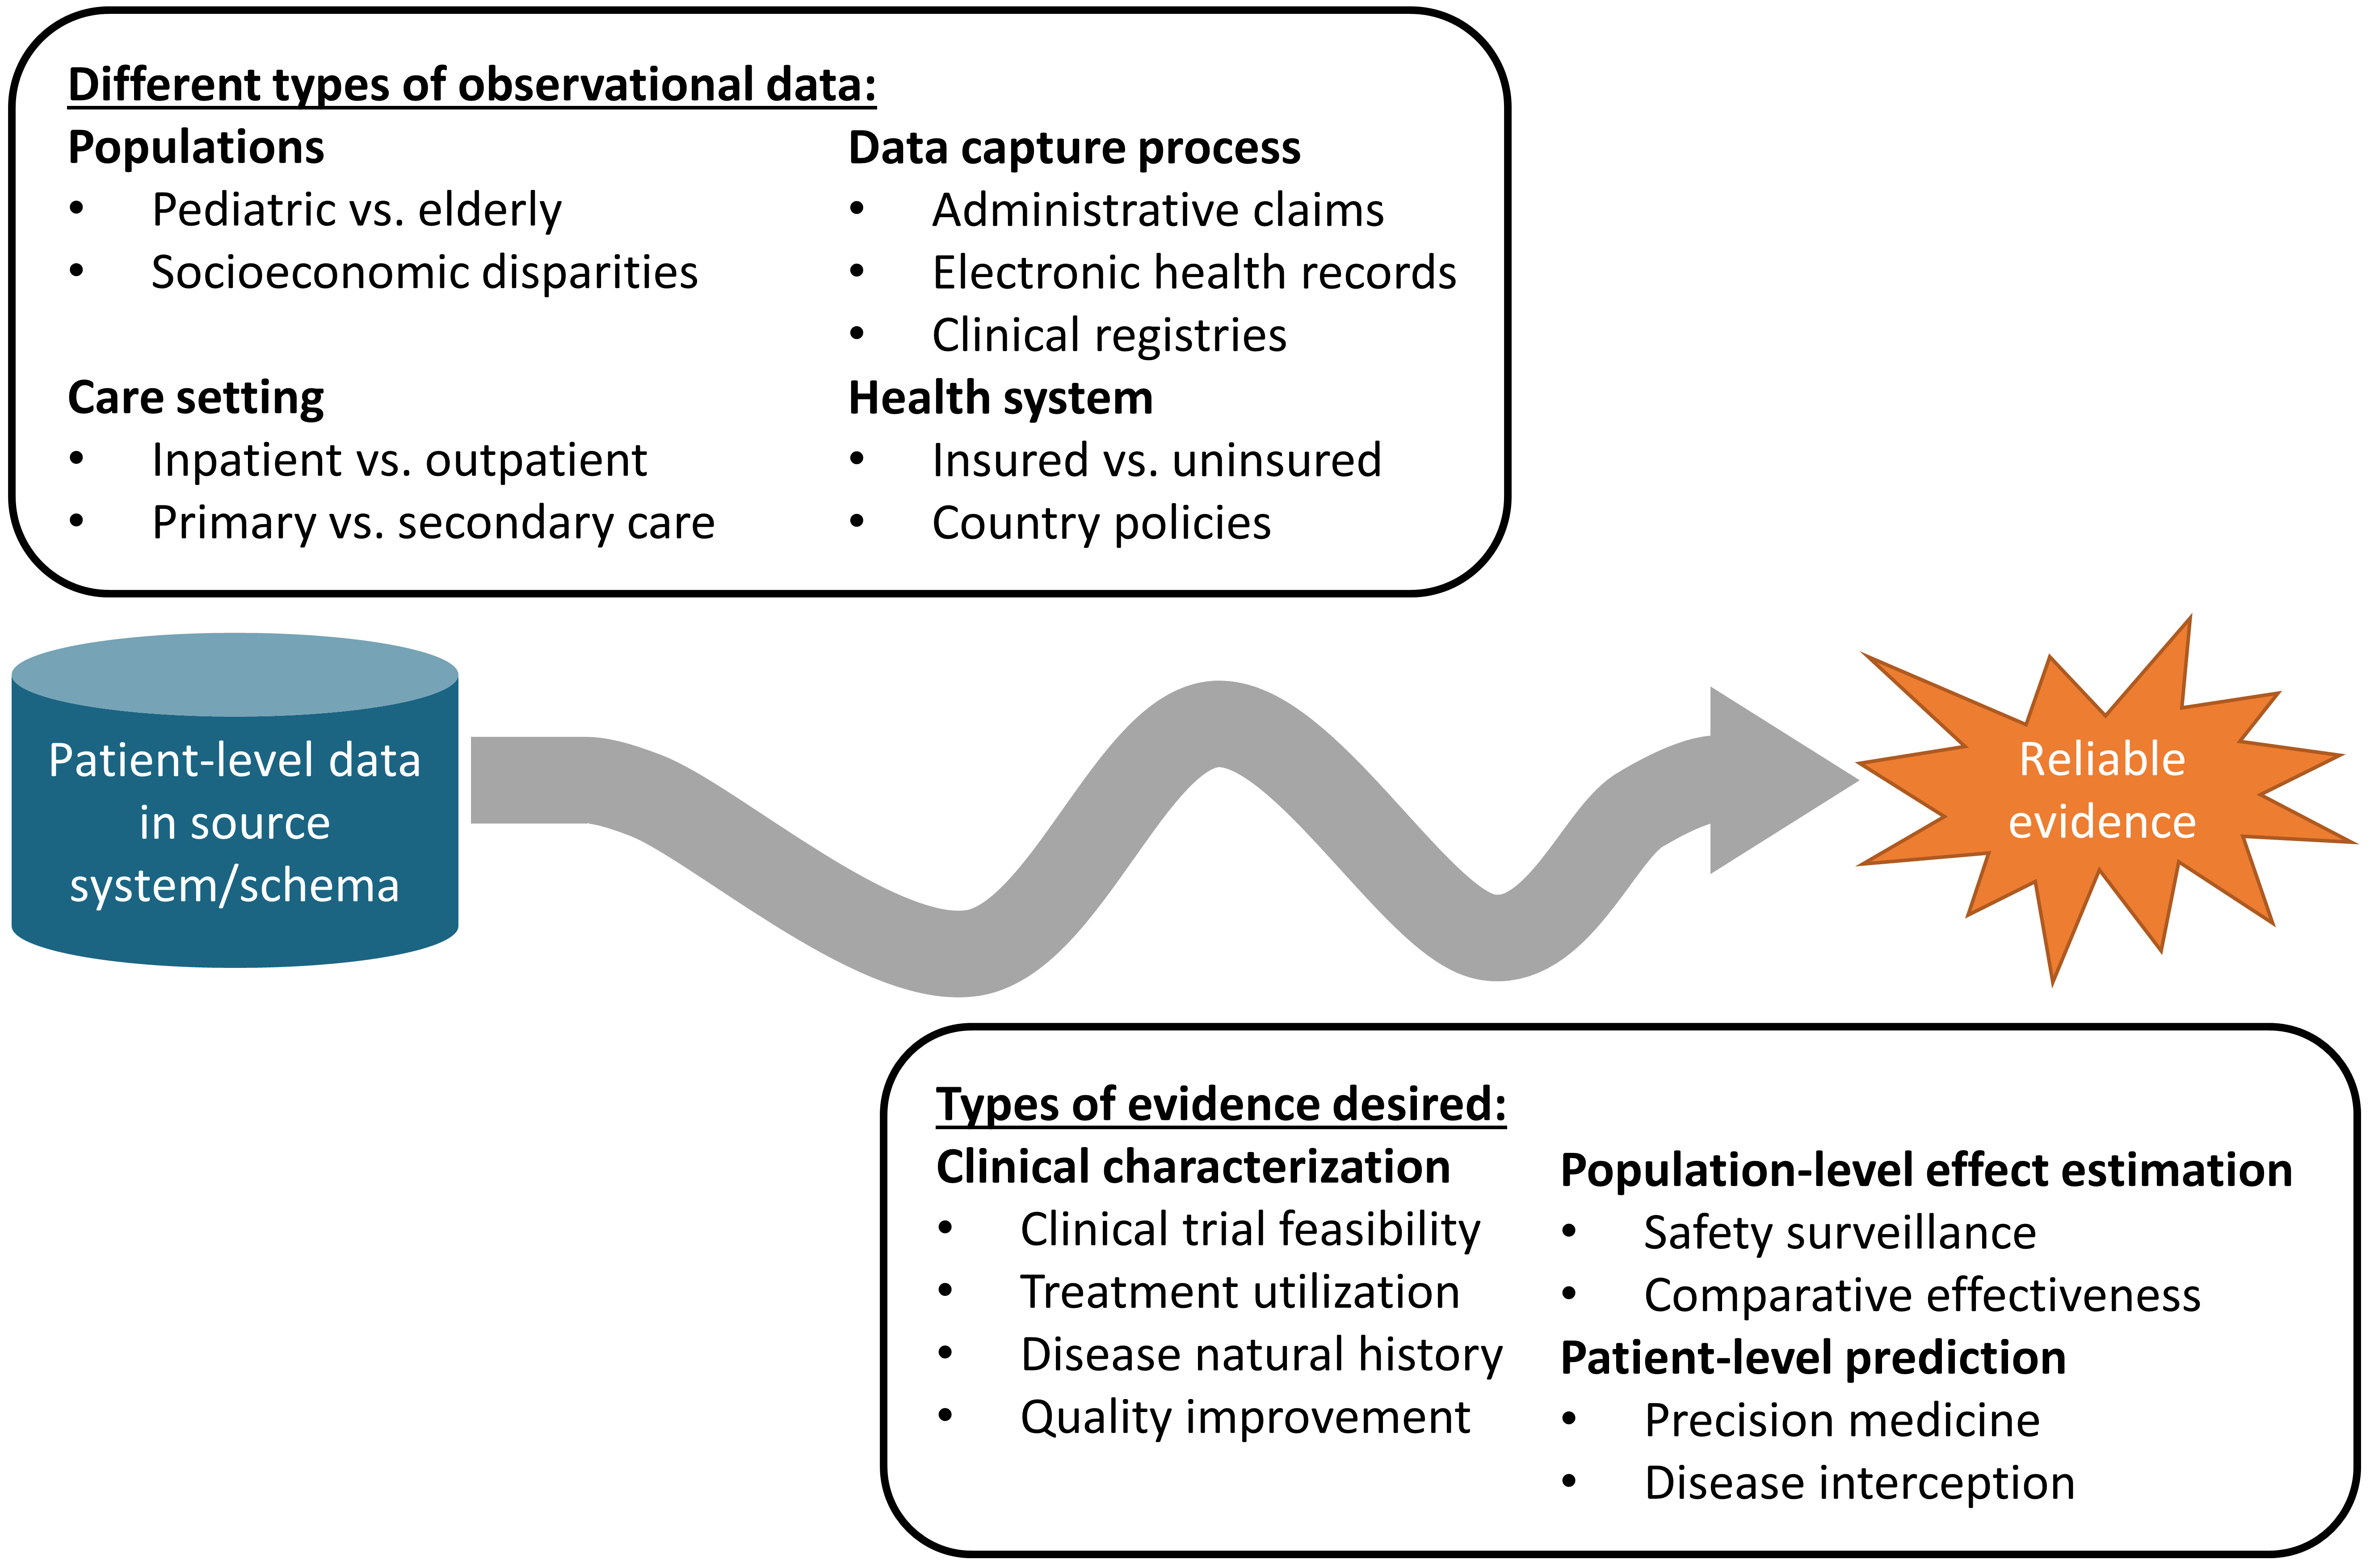
\includegraphics[width=1\linewidth]{images/OhdsiCommunity/datajourney} 

}

\caption{데이터에서 근거로의 여정}\label{fig:datajourney}
\end{figure}

원천 시스템에는 다양한 환자 수준의 데이터를 수집하는 여러 유형의 관찰형
데이터베이스 observational database가 있다. 이 데이터베이스는 서로 다른
의료 시스템 내부의 인구, 치료 설정 및 데이터 수집 프로세스의 이질성만큼
다양하다. 의사 결정에 도움이 될 수 있는 다양한 유형의 근거가 있으며,
분석 방법론에 따라 임상적 특성 분석 clinical characterization, 인구 수준
추정 population-level estimation 및 환자 수준 예측 patient-level
prediction으로 분류할 수 있다. 출발지(원천 데이터) 및 원하는
목적지(근거) 와는 별도로, 여정을 수행하는 데 필요한 광범위한 임상, 과학
및 기술 역량들은 문제를 더욱 복잡하게 만든다. 보험 청구나 진료 과정이
데이터로 수집되면서 보건 정책이나 보험 환급과 관련된 행동 동기들로 인해
데이터 수집 및 정제 과정에서 발생할 수 있는 비뚤림을 비롯하여 환자와
의료 제공자 간의 진료현장에서 원천 데이터가 수집되는 전반적인 과정에
대한 철저한 의료정보학적 이해도 필요하다. 임상적 의문으로부터 해답을
도출하는 데 적합한 관찰 연구 설계를 설계하기 위해선 역학 원칙과 통계적
방법도 숙지하고 있어야 한다. 수백만 명의 환자의 수년간의 종적 추적에
걸친 수십억 건의 임상 관찰을 가진 데이터 세트에 대해 계산적으로 효율적인
데이터 처리 알고리즘을 구현하고 실행할 수 있는 기술적 능력 역시
필요하다. 관찰형 연구를 통해 습득한 내용을 다른 근거와 통합하고, 이
새로운 지식이 건강 정책 및 임상 관행에 어떤 영향을 미칠지 고려하기
위해서는 임상 지식 또한 필요하다. 따라서, 한 개인이 데이터를 이용하여
근거를 성공적으로 만들어 내는 데 필요한 기술과 자원을 모두 보유하는 것은
매우 드문 일이다. 따라서 이용 가능한 최선의 데이터를 가장 적절한
방법으로 분석하여 모든 이해당사자가 그들의 의사결정 과정에 믿고 사용할
수 있는 근거를 생산하기 위해서는, 종종 많은 개인이나 기관과의 협력을
필요로 한다.

\section{OMOP (Observational Medical Outcomes
Partnership)}\label{omop-observational-medical-outcomes-partnership}

협력 관찰형 연구 모델의 주목할만한 예시로 OMOP(Observational Medical
Outcomes Partnership)이 있다. OMOP은 미국 식품의약국 FDA이 주관하고,
미국 국립 보건원 National Institutes of Health 관리하에 학술 연구자,
보건 데이터 파트너 및 협력 제약사간의 컨소시엄으로 구성되었으며, 관찰형
보건의료 데이터를 이용하여 능동적 의료 제품 안전성 감시의 발전을
꾀하고자 만들어진 민관 협력체였다. \citep{stang2010omop} OMOP은 다수의
이해관계자 간의 거버넌스 구조를 확립했고, 다수의 청구자료 및 전자 의무
기록 데이터베이스에 적용하여 참인 약물 안전성 연관성과 거짓 양성 소견을
식별할 수 있는 대안적인 역학 설계 및 통계 방법의 성능을 경험적으로
검증하는 일련의 방법론적 실험을 설계하였다.

분산된 관찰형 데이터베이스를 통해 연구를 진행하면서 기술적인 난제를
인식하고, 연구진들은 데이터의 구조, 내용 및 용어를 표준화하여 하나의
통계 분석 코드가 모든 데이터 파트너에서 공통으로 사용될 수 있도록, OMOP
공통 데이터 모델 Common Data Model(CDM)을 설계하였다.
\citep{overhage2012cdm} OMOP 실험은 공통 데이터 모델과 표준화된 어휘를
확립하는 것이 가능하다는 것을 증명하였으며, 이는 서로 다른 의료체계에서
다른 용어체계를 통해서 생성된 다른 데이터 유형을 수용하여 기관 간 협업과
계산적으로 효율적인 분석을 용이하게 할 수 있는 방식으로 구현되었다.

OMOP는 처음부터 오픈 사이언스 정책을 채택하여 연구 설계, 데이터 표준,
분석 코드, 경험적 결과 등 모든 작업의 결과를 공공에 배포함으로써
투명성을 증진하고, OMOP이 수행하고 있는 연구에 대한 신뢰를 쌓을 뿐
아니라, 또한 다른 이들의 연구 목적을 위하여 발전할 수 있도록 하였다.
OMOP의 원래 초점은 약물 안전성이었지만, 의학적 개입이나 보건 시스템
정책에 대한 비교효과연구를 포함하여 다양한 분석 사용사례를 지원하기 위해
지속해서 발전했다.

OMOP은 대규모의 경험적 실험을 완성하는 데 성공하였고,
\citep{ryan2012omop, ryan2013omop} 방법론적인 혁신을 만들고,
\citep{schuemie_2014} 관찰형 데이터를 이용한 안정성에 관련된 의사결정에
유용한 지식 생성을 위한 적절한 방법론을
제시하였다.\citep{madigan_2013, madigan2013design} OMOP 프로젝트는
종료되었지만, 오픈 사이언스 원칙과 함께 OMOP의 유산은 OHDSI가 이어
받았다.

OMOP 프로젝트가 FDA의 능동 감시에 도움을 줄 수 있는 관찰형 연구를
완료하고 종료된 이후, 사람들은 OMOP 여정의 끝이 새로운 여정의 시작이
되어야 한다고 생각했다. OMOP의 방법론적 연구가 관찰형 데이터에서
생성되는 근거의 품질을 명시적으로 개선할 수 있는 모범 사례best
practice를 제시하였지만, 그러한 모범 사례의 채택은 느렸다. 몇 가지
장애물들이 있었는데, 1) 방법론적인 혁신을 내세우기 전 관찰형 자료의
품질에 대한 근본적인 우려 2) 방법론적 문제와 해결책에 대한 불충분한
개념적 이해 3) 개별 데이터 파트너의 로컬 환경 내에서 솔루션을 독립적으로
구현할 수 없다는 점 4) 이러한 접근방식이 다른 연구자들이 관심을 가지고
있는 임상적 문제에 적용 가능한지에 대한 불확실성 등이었다. 이러한 모든
장애물에 대해 변화를 만들기 위해서는 한 개인의 힘이 아니라, 여러 사람이
협력하여야만 한다는 것을 깨달을 수 있었다. 다음과 같은 협력이 필요했다:

\begin{itemize}
\tightlist
\item
  기초 데이터 품질에 대한 신뢰도를 높이며 구조, 콘텐츠 및 의미론적
  일관성을 촉진하여 표준화된 분석이 가능하도록 개방형 커뮤니티open
  community의 데이터 구조, 어휘 및 추출 변환 적재Extract-Transform-Load
  (ETL) 표준규약 구축을 위한 협업
\item
  약물 안전성 연구 외에도 clinical characterization, population-level
  effect estimation, patient-level prediction을 위한 보다 광범위한 모범
  사례를 확립하기 위한 협업. 방법론적 연구를 통해 입증된 과학적 모범
  사례를 코드로 구현하고 연구자들이 쉽게 채택할 수 있는 오픈 소스 분석
  소프트웨어 개발에 대한 협업
\item
  주요한 보건 문제를 해결할 공통의 질문에 대한 임상적용을 위한
  협업으로서, 커뮤니티를 아울러서 데이터에서 근거로의 여정을 총괄적으로
  인도해줄 수 있는 협업체계
\end{itemize}

이러한 통찰을 통해, OHDSI가 태어났다.

\section{개방형 과학 공동체로서의 OHDSI}\label{---ohdsi}

OHDSI(Observational Health data Sciences and Informatics)는 보다 더 나은
의료 결정과 더 나은 보건 관리를 촉진할 수 있는 과학적 근거를 공동으로
생성하도록 함으로써 보건 수준을 향상하는 것을 목표로 하는 개방형 과학
공동체다. \citep{Hripcsak2015} OHDSI는 관찰형 건강 데이터(observational
health data)의 적절한 사용에 대한 과학적 모범 사례를 확립하기 위한
방법론적 연구를 수행하고, 이러한 연구방법론을 일관되고 투명하며 재현
가능한 솔루션으로 코드화하는 오픈 소스 분석 소프트웨어를 개발하여,
보건의료 정책 및 환자 치료에 도움이 될 수 있는 임상적 근거를 마련하는
데에 적용할 수 있도록 노력한다.

\subsection{OHDSI의 사명 Mission}\label{ohdsi--mission}

더 나은 의학적 결정과 의료 발전을 촉진할 수 있는 근거를 상호협력하여
생성할 수 있도록 공동체에 힘을 실어줌으로써 보건을 개선한다.

\begin{quote}
To improve health by empowering a community to collaboratively generate
the evidence that promotes better health decisions and better care.
\index{mission}
\end{quote}

\subsection{OHDSI의 이상 Vision}\label{ohdsi--vision}

관찰형 연구를 통해 건강과 질병에 대한 포괄적인 이해가 가능한 세상

\begin{quote}
A world in which observational research produces a comprehensive
understanding of health and disease. \index{vision}
\end{quote}

\subsection{OHDSI의 목표 Objectives}\label{ohdsi--objectives}

\begin{itemize}
\tightlist
\item
  \textbf{혁신 Innovation}: 관찰형 연구는 파괴적 사유를 통해서 가장
  혜택을 얻을 수 있는 분야이다. 우리는 우리의 업무에 새로운 방법론적인
  접근을 적극적으로 찾고 격려한다.
\end{itemize}

\begin{quote}
Observational research is a field which will benefit greatly from
disruptive thinking. We actively seek and encourage fresh methodological
approaches in our work.
\end{quote}

\begin{itemize}
\tightlist
\item
  \textbf{재현 Reproducibility}: 보건향상을 위해서는 정확하고
  재현가능하며 잘 보정된 근거가 필요하다.
\end{itemize}

\begin{quote}
Accurate, reproducible, and well-calibrated evidence is necessary for
health improvement.
\end{quote}

\begin{itemize}
\tightlist
\item
  \textbf{공동체 Community}: 우리는 OHDSI에 적극적으로 참여하는 모든
  사람 (환자, 의료직 전문가, 연구자, 또는 단순히 우리의 주장을 믿는
  사람) 을 환영한다.
\end{itemize}

\begin{quote}
Everyone is welcome to actively participate in OHDSI, whether you are a
patient, a health professional, a researcher, or someone who simply
believes in our cause.
\end{quote}

\begin{itemize}
\tightlist
\item
  \textbf{협력 Collaboration}: 우리는 우리 공동체 참여자들의 현실적
  요구를 최우선적으로 다루기 위해서 함께 일한다.
\end{itemize}

\begin{quote}
We work collectively to prioritize and address the real world needs of
our community's participants.
\end{quote}

\begin{itemize}
\tightlist
\item
  \textbf{개방 Openness}: 우리는 방법론, 도구, 우리가 생성하는 근거 등
  우리 공동체의 모든 진행사항을 개방하고 공개적으로 접근가능할 수 있도록
  최대한 노력한다.
\end{itemize}

\begin{quote}
We strive to make all our community's proceeds open and publicly
accessible, including the methods, tools and the evidence that we
generate.
\end{quote}

\begin{itemize}
\tightlist
\item
  \textbf{선행 Beneficence}: 우리는 우리 공동체에 속한 개인과 기관의
  권리를 보호하기 위해서 항상 노력한다.
\end{itemize}

\begin{quote}
We seek to protect the rights of individuals and organizations within
our community at all times.
\end{quote}

\index{objectives}

\hypertarget{ohdsi-}{\section{OHDSI의 역사}\label{ohdsi-}}

OHDSI는 2014년 설립된 이래 성장을 지속하여 컴퓨터 과학, 역학, 통계,
의생명 정보학, 보건 정책 및 임상 의학 등 다양한 분야를 대표하는 학계,
의료 제품 산업, 규제 기관, 정부, 보험자, 기술 제공자, 의료 시스템,
임상의사 및 환자 집단 등 2,500명 이상의 다양한 이해관계자가 온라인
포럼에서 활동하고 있다. OHDSI 협력체로써 자발적으로 보고한 기관 및
데이터베이스의 리스트는 OHDSI 웹사이트에서 확인할 수 있다. \footnote{\url{https://www.ohdsi.org/who-we-are/collaborators/}}
OHDSI 협력자 지도 (Figure \ref{fig:collaboratormap}) 는 폭넓은 국제
공동체로서의 다양성을 상기시킨다.

\begin{figure}

{\centering 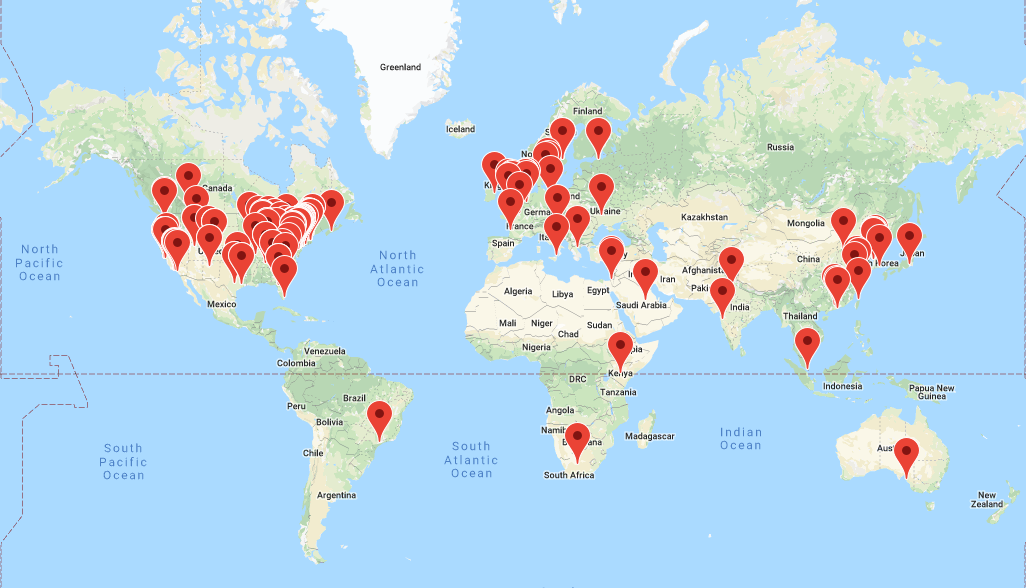
\includegraphics[width=1\linewidth]{images/OhdsiCommunity/mapOfCollaborators} 

}

\caption{2019년 8월 기준 OHDSI 협력자 지도}\label{fig:collaboratormap}
\end{figure}

OHDSI는 OMOP-CDM이라는 개방형 공동체 데이터 표준 기반으로 2019년 8월
기준으로 20여 개국, 100개 이상의 의료 데이터베이스들로 구성된 분산
연구망 distributed research network(DRN)을 구축했다. 분산 연구망이란
환자 수준의 데이터를 개인이나 조직 간에 공유할 필요가 없다는 것을
의미한다. 분산 연구망에서는, 데이터를 기관 폐쇄망 안에 두고 연구자는
프로토콜 형태의 분석 코드/프로그램을 공유한다. 데이터 파트너들은
연구자의 요청에 따라 기관 안에서 연구 프로토콜을 실행해 자동으로
생성되는 요약 집합정보 (평균, 합, 표준편차, 교차비, 위험도 등) 만
연구자에게 회신하는 방식으로, 연구자는 폐쇄망 안에 있는 환자의 개별
정보를 보거나 취득하지 않는다. OHDSI 분산망에서 각 데이터 파트너는 환자
수준 데이터의 사용에 대한 완전한 자율성을 유지하고, 각 기관의 데이터
거버넌스 정책을 지속해서 준수할 수 있다.

OHDSI 개발자 커뮤니티는 3가지의 사용 사례를 지원하기 위해 OMOP CDM 위에
다음 3가지의 강력한 오픈 소스 분석 소프트웨어 라이브러리를 구축하였는데
이는 다음과 같다. 1) 임상적 특성 분석(clinical characterization): 질병의
자연 경과, 치료 행태 및 질 향상을 위한 임상 특성 분석 2) 인구 수준 추정
(population-level effect estimation): 의약품 안전성 감시 및 비교 효과
연구에서의 인과성 분석 3) 환자 수준 예측(patient-level prediction):
기계학습 알고리즘을 활용한 정밀 의학 또는 의료 개입. OHDSI 개발자들은
OMOP CDM의 채택, 데이터 품질 평가, OHDSI 네트워크 연구의 촉진을 지원하는
애플리케이션을 개발하고 있다. 이러한 소프트웨어에는 R과 Python에 내장된
백 엔드 통계 패키지 및 HTML과 Javascript로 개발된 프론트엔드 웹
어플리케이션이 포함된다. 모든 OHDSI 소프트웨어들은 오픈 소스 정책을
채택하여 Github을 통해 공개된다. \footnote{\url{https://github.com/OHDSI}}

오픈 소스 소프트웨어들과 함께, OHDSI의 개방형 과학 공동체적 접근은
관찰형 연구의 발전을 가능하게 했다. 첫 번째 OHDSI 네트워크 연구는 당뇨,
우울증, 고혈압의 3가지 만성 질병에 대한 치료 패턴을 분석하는 것이었다.
PNAS(Proceedings of the National Academy of Science)에 출판된 연구는, 그
때까지 수행된 최대 규모의 관찰형 연구로써 11개의 데이터베이스에서 2억
5천만 명의 환자 데이터를 이용하여 이전에 보고된 적 없는 치료 패턴의
지역적 차이 및 환자별 치료 선택에 대한 이질성에 대해 발표하였다.
\citep{Hripcsak7329} OHDSI는 교란변수를 통제하는 새로운 통계적 방법론을
제시하였고, \citep{tian_2018} 인과성 검증 능력에 대해 검증하였고,
\citep{schuemie_2018} 이러한 방법론을 뇌전증 약제의 개별 안전성 연구
\citep{duke_2017} 및 당뇨병의 이차 약제의 비교 효과 연구
\citep{vashisht_2018}, 우울증 치료의 대규모 비교 효과 연구
\citep{schuemie_2018b}, 고혈압 환자의 이제 병합 요법의 비교 효과
연구\citep{you_olmesartan_2019}, 대규모 고혈압 약제 비교
연구\citep{suchard_comprehensive_2019} 에 활용하였다. OHDSI 공동체는
또한 관찰형 보건의료 데이터의 기계학습 알고리즘을 활용한 프레임 워크를
구축 \citep{reps2018} 하여 다양한 치료 분야에 활용하였다.
\citep{johnston_2019, cepeda_2018, reps_2019}

\hypertarget{ohdsi-}{\section{OHDSI와의 협업}\label{ohdsi-}}

OHDSI는 근거를 생성하기 위해 협업을 강화하는 것을 목표로 하는
공동체인데, OHDSI 참가자가 된다는 것은 무엇을 의미하는가? 만약 당신이
OHDSI의 사명을 믿고 데이터에서 근거에 이르는 여정의 어디든지 기여를 하는
데 관심이 있다면, OHDSI는 당신을 위한 공동체가 될 수 있다. OHDSI
참가자는 보건 의료 데이터에 접근이 가능하고, 이를 활용해 의학적 근거를
생성하고 싶은 개인일 수 있다. OHDSI 참가자는 과학적 모범 사례를 수립하고
대안적 접근법을 평가하는 데 관심이 있는 방법론 연구자일 수 있다. OHDSI
참가자는 OHDSI의 타 연구자들이 사용할 수 있는 도구를 만들기 위해
프로그래밍 기술을 적용하는 데 관심이 있는 소프트웨어 개발자일 수 있다.
OHDSI 참가자는 중요한 의학 보건학적 질문을 가지고 있고 논문 발표 등을
통해 그러한 질문들에 대한 근거를 더욱 더 큰 의료 커뮤니티에 제공하고자
하는 임상 연구자일 수 있다. OHDSI 참가자는 공공 보건을 위해 이러한
공통적인 사명과 가치를 믿고 해당 지역의 공동체가 OHDSI 관련 교육과
심포지엄 개최를 포함하여, 그 임무를 지속할 수 있도록 자원을 제공하는
개인 또는 단체일 수도 있다. 당신의 배경이나 소속과 관계없이, OHDSI는
개개인이 공통의 목적을 위해 함께 일할 수 있는 공동체가 되기를 추구하고
있으며, 각 개인이 공동으로 의료를 발전시킬 수 있는 기여를 하고 있다. 이
여정에 함께하고 싶다면, \ref{WhereToBegin}장 (``OHDSI 시작하기'') 을
통해 어떻게 시작하는지 배울 수 있다.

\section{한국 OHDSI의 역사}\label{-ohdsi-}

OMOP의 창립자 중 한명인 Martijn Schuemie는 OMOP의 연구성과 중 하나로서
관찰형 자료에서 confounding by indication을 찾을 수 있는 LEOPARD
알고리즘을 고안하였고, 2010년 남아프리카 케이프타운에서 열린
세계의료정보학회(IMIA)에서 그 내용을 발표하였다. 당시 세계의료정보학회에
참석하였던 박래웅은 우연히 Martijn Schuemie의 LEOPARD 알고리즘과 OMOP을
접하게 되었고 강한 흥미와 유대감을 느꼈다. 이후 그는 2012년 국내 4개
대학병원의 다기관 임상의료정보 통합시스템 개발을 진행하였고 이를 위해
자체적으로 고안한 CDM을 적용하였다. 2013년 세계약물역학학회(ICPE)가
2013년 9월 캐나타 몬트리올에서 열렸고 이 학회에서 다시 만난 Martijn
Schuemie, Patrick Ryan과 박래웅은 각자 진행하던 프로젝트에 대해서
논의하였고 향후 긴밀한 협조를 결의하였다. 이후 그는 빠른시간내에
아주대병원 전자의무기록을 CDM으로 변환완료하고 2014년 OHDSI의 결성을
알리는 콜롬비아대학에서 열린 첫번째 face-to-face 모임에 참여하면서
변환완료된 아주대병원의 CDM과 Achilles 웹페이지를 전격 공개하였다. 미국
이외의 국가에서 변환된 첫번째 CDM이며 전세계에서 첫번째로 공개된
Achilles 페이지였다.

\begin{figure}

{\centering 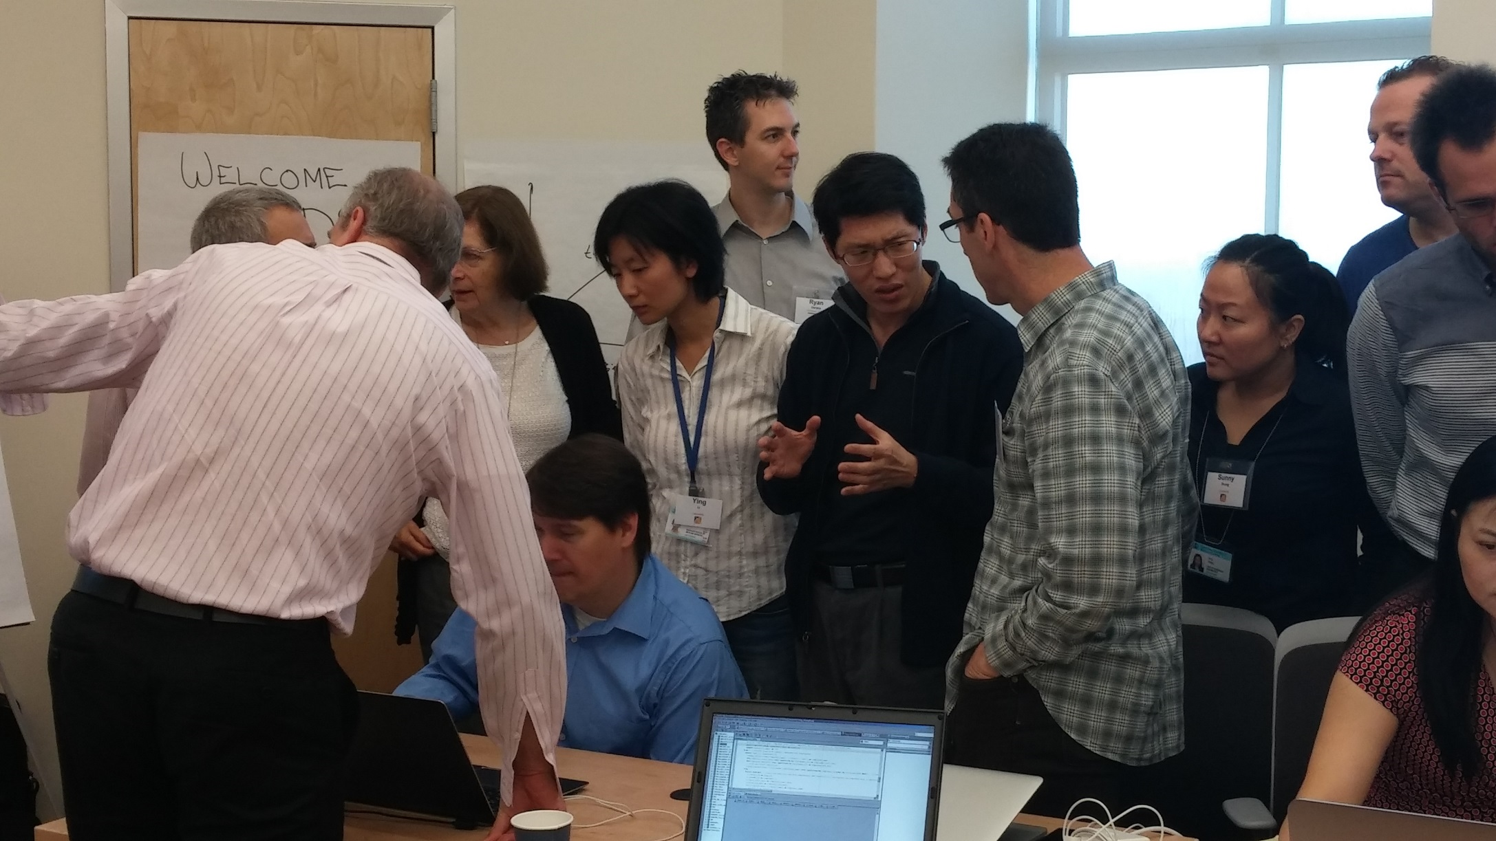
\includegraphics[width=0.8\linewidth]{images/OhdsiCommunity/2014f2fmeeting_korea} 

}

\caption{2014년 최초 개최된 OHDSI Face to Face 미팅에서 아주대학교병원의 CDM과 Achilles웹페이지를 소개하였다. 사진의 좌측하단에 Christopher Knoll이 아주대 CDM Achilles화면을 살펴보고 있으며 많은 참석자들이 각별한 관심을 보였다.}\label{fig:OHDSIf2f2014}
\end{figure}

그는 2014년 6월 이후 본격적으로 한국사회에 OHDSI를 알리기 시작하였고,
이후 국민건강보험공단을 시작으로 가천길병원 등이 OHDSI에 참여하기
시작하였다. 이후 계속 국내외에서 OMOP-CDM, OHDSI 전파를 위해 노력한
결과, 2016년부터는 최초로 국제 OHDSI committee에서 개별 국가를 위한 포럼
\href{http://forums.ohdsi.org/c/For-collaborators-wishing-to-communicate-in-Korean}{Korean
chapter} 을 개설하고, 한국의 OHDSI 참여가 본격화 되었다. 첫 한국 국제
OHDSI 심포지엄은 2017년 3월 아주대학교에서 튜토리얼, 리더십 미팅을
포함하여 3일간 개최되었다.

\begin{figure}
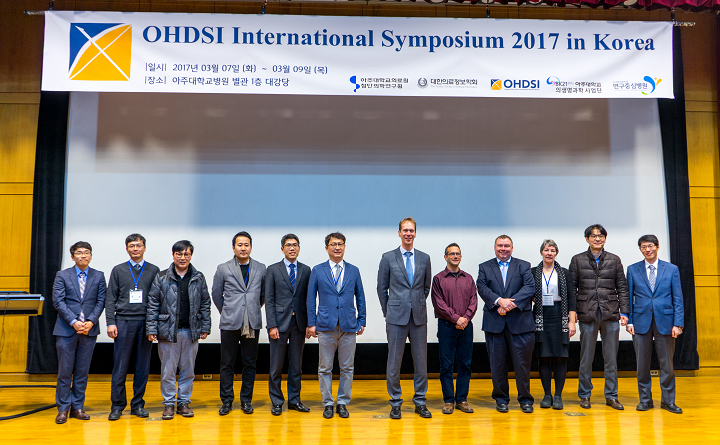
\includegraphics[width=0.8\linewidth]{images/OhdsiCommunity/DSC01956} \caption{2017년 한국에서의 OHDSI 국제 심포지엄}\label{fig:OHDSIInternationalSymposium2017inKorea1}
\end{figure}\begin{figure}
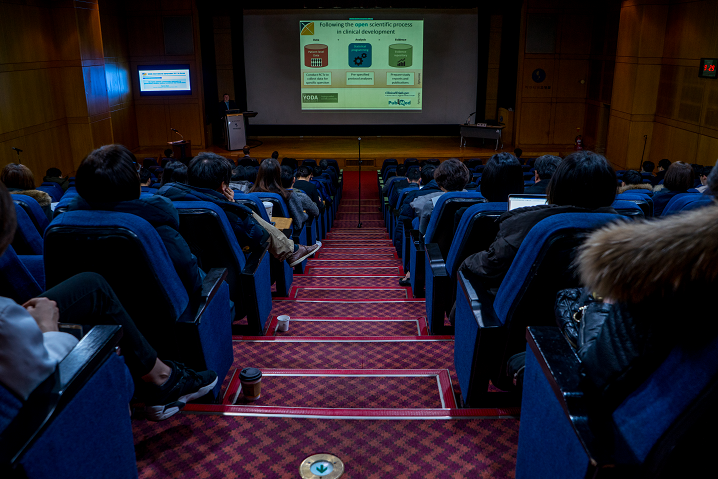
\includegraphics[width=0.8\linewidth]{images/OhdsiCommunity/DSC01861} \caption{2017년 한국에서의 OHDSI 국제 심포지엄}\label{fig:OHDSIInternationalSymposium2017inKorea1}
\end{figure}

\begin{figure}
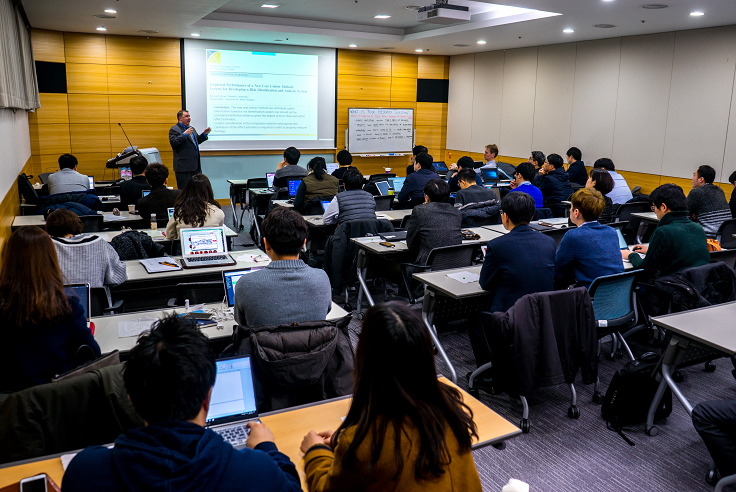
\includegraphics[width=0.8\linewidth]{images/OhdsiCommunity/DSC02166} \caption{2017년 한국에서의 OHDSI 국제 심포지엄 튜토리얼}\label{fig:OHDSIInternationalSymposium2017inKorea2}
\end{figure}

한국 OHDSI 네트워크에 참여를 희망하는 병원 관계자들과 함께 2017년 3월
7일 첫 번째 리더십 미팅을 가진 후 현재까지 2달마다 전국의
의과대학/병원을 순회하며 총 15회 이상의 한국 OHDSI 리더십 미팅을
개최하며 OHDSI 전파 및 상호 협력을 꾀하고 있다.

\section{요약}

\BeginKnitrBlock{rmdsummary}
\begin{itemize}
\item
  OHDSI의 사명은 참여 공동체의 상호협력 하에 의료 발전을 촉진하는 근거를
  생성하는 능력을 부여하는 것이다.
\item
  OHDSI의 이상은 혁신성, 재현성, 공동체 정신, 개방성, 협력 정신, 선행의
  정신을 바탕으로 의료 빅데이터의 분석을 통해 세계에 건강과 질병에 대한
  포괄적인 이해를 제공하는 것이다.
\item
  OHDSI 참가자들은 개방형 공동체로서의 데이터 표준, 방법론 연구,
  오픈소스 분석 소프트웨어 개발 및 임상적 적용을 통해 데이터로부터
  근거로의 여정을 발전시키고자 노력한다.
\end{itemize}
\EndKnitrBlock{rmdsummary}

\chapter{OHDSI 시작하기}\label{WhereToBegin}

\emph{Chapter leads: Hamed Abedtash \& Kristin Kostka}

\begin{quote}
``천리길도 한 걸음부터'' - 노자
\end{quote}

OHDSI 커뮤니티는 학계, 산업계 및 정부 기관 전반에 걸쳐 다양한
이해관계자들을 대표하고 있다. 본 커뮤니티의 작업으로 의료 시스템뿐
아니라 환자, 의료제공자, 연구자들을 포함한 다양한 개인들과 기관들이
혜택을 받게 된다. 이러한 이점은 의료 데이터를 더 유용하도록 개선할 뿐만
아니라 의료데이터 분석의 질을 향상함으로써 얻어지게 된다. 관찰형 연구는
파괴적인 생각disruptive thinking으로부터 크게 혜택을 받을 수 있는
분야이다. 이 분야에서는 적극적인 새로운 방법론적 도입이 필요하다.
\index{community}

\section{여정에 동참하십시오}\label{-}

환자, 의료 전문가, 연구자 혹은 단순히 OHDSI의 목적에 동감하는 사람이면
누구든지 OHDSI 커뮤니티에 적극적으로 참여할 수 있다. OHDSI는 포용적
멤버십 모델을 추구하며 OHDSI의 공동연구자가 되기 위한 멤버십 비용은
없다. 참여를 원하는 사람은 단지 손을 들어서 매년 OHDSI 멤버십 카운트에
포함되면 된다. 참여는 전적으로 자의에 의한 것이며 매주 커뮤니티의
네트워크 스터디나 OHDSI 작업 그룹에 참여하는 것만으로도 충분하다. 꼭
데이터를 보유하고 있어야만 OHDSI 커뮤니티의 액티브 멤버가 되는 것은
아니다. 본 커뮤니티는 데이터 보유자, 연구자, 헬스케어 제공자, 환자와
소비자 모두에게 도움을 주고자 한다. 공동연구자의 프로필은 OHDSI
웹사이트에서 관리되고 정기적으로 업데이트되고 있다. 멤버십은 OHDSI
커뮤니티 원격회의, 워크그룹, 지역별 모임을 통해 육성되고 있다.
\index{join the journey} \index{workgroups} \index{chapters}

\begin{figure}

{\centering 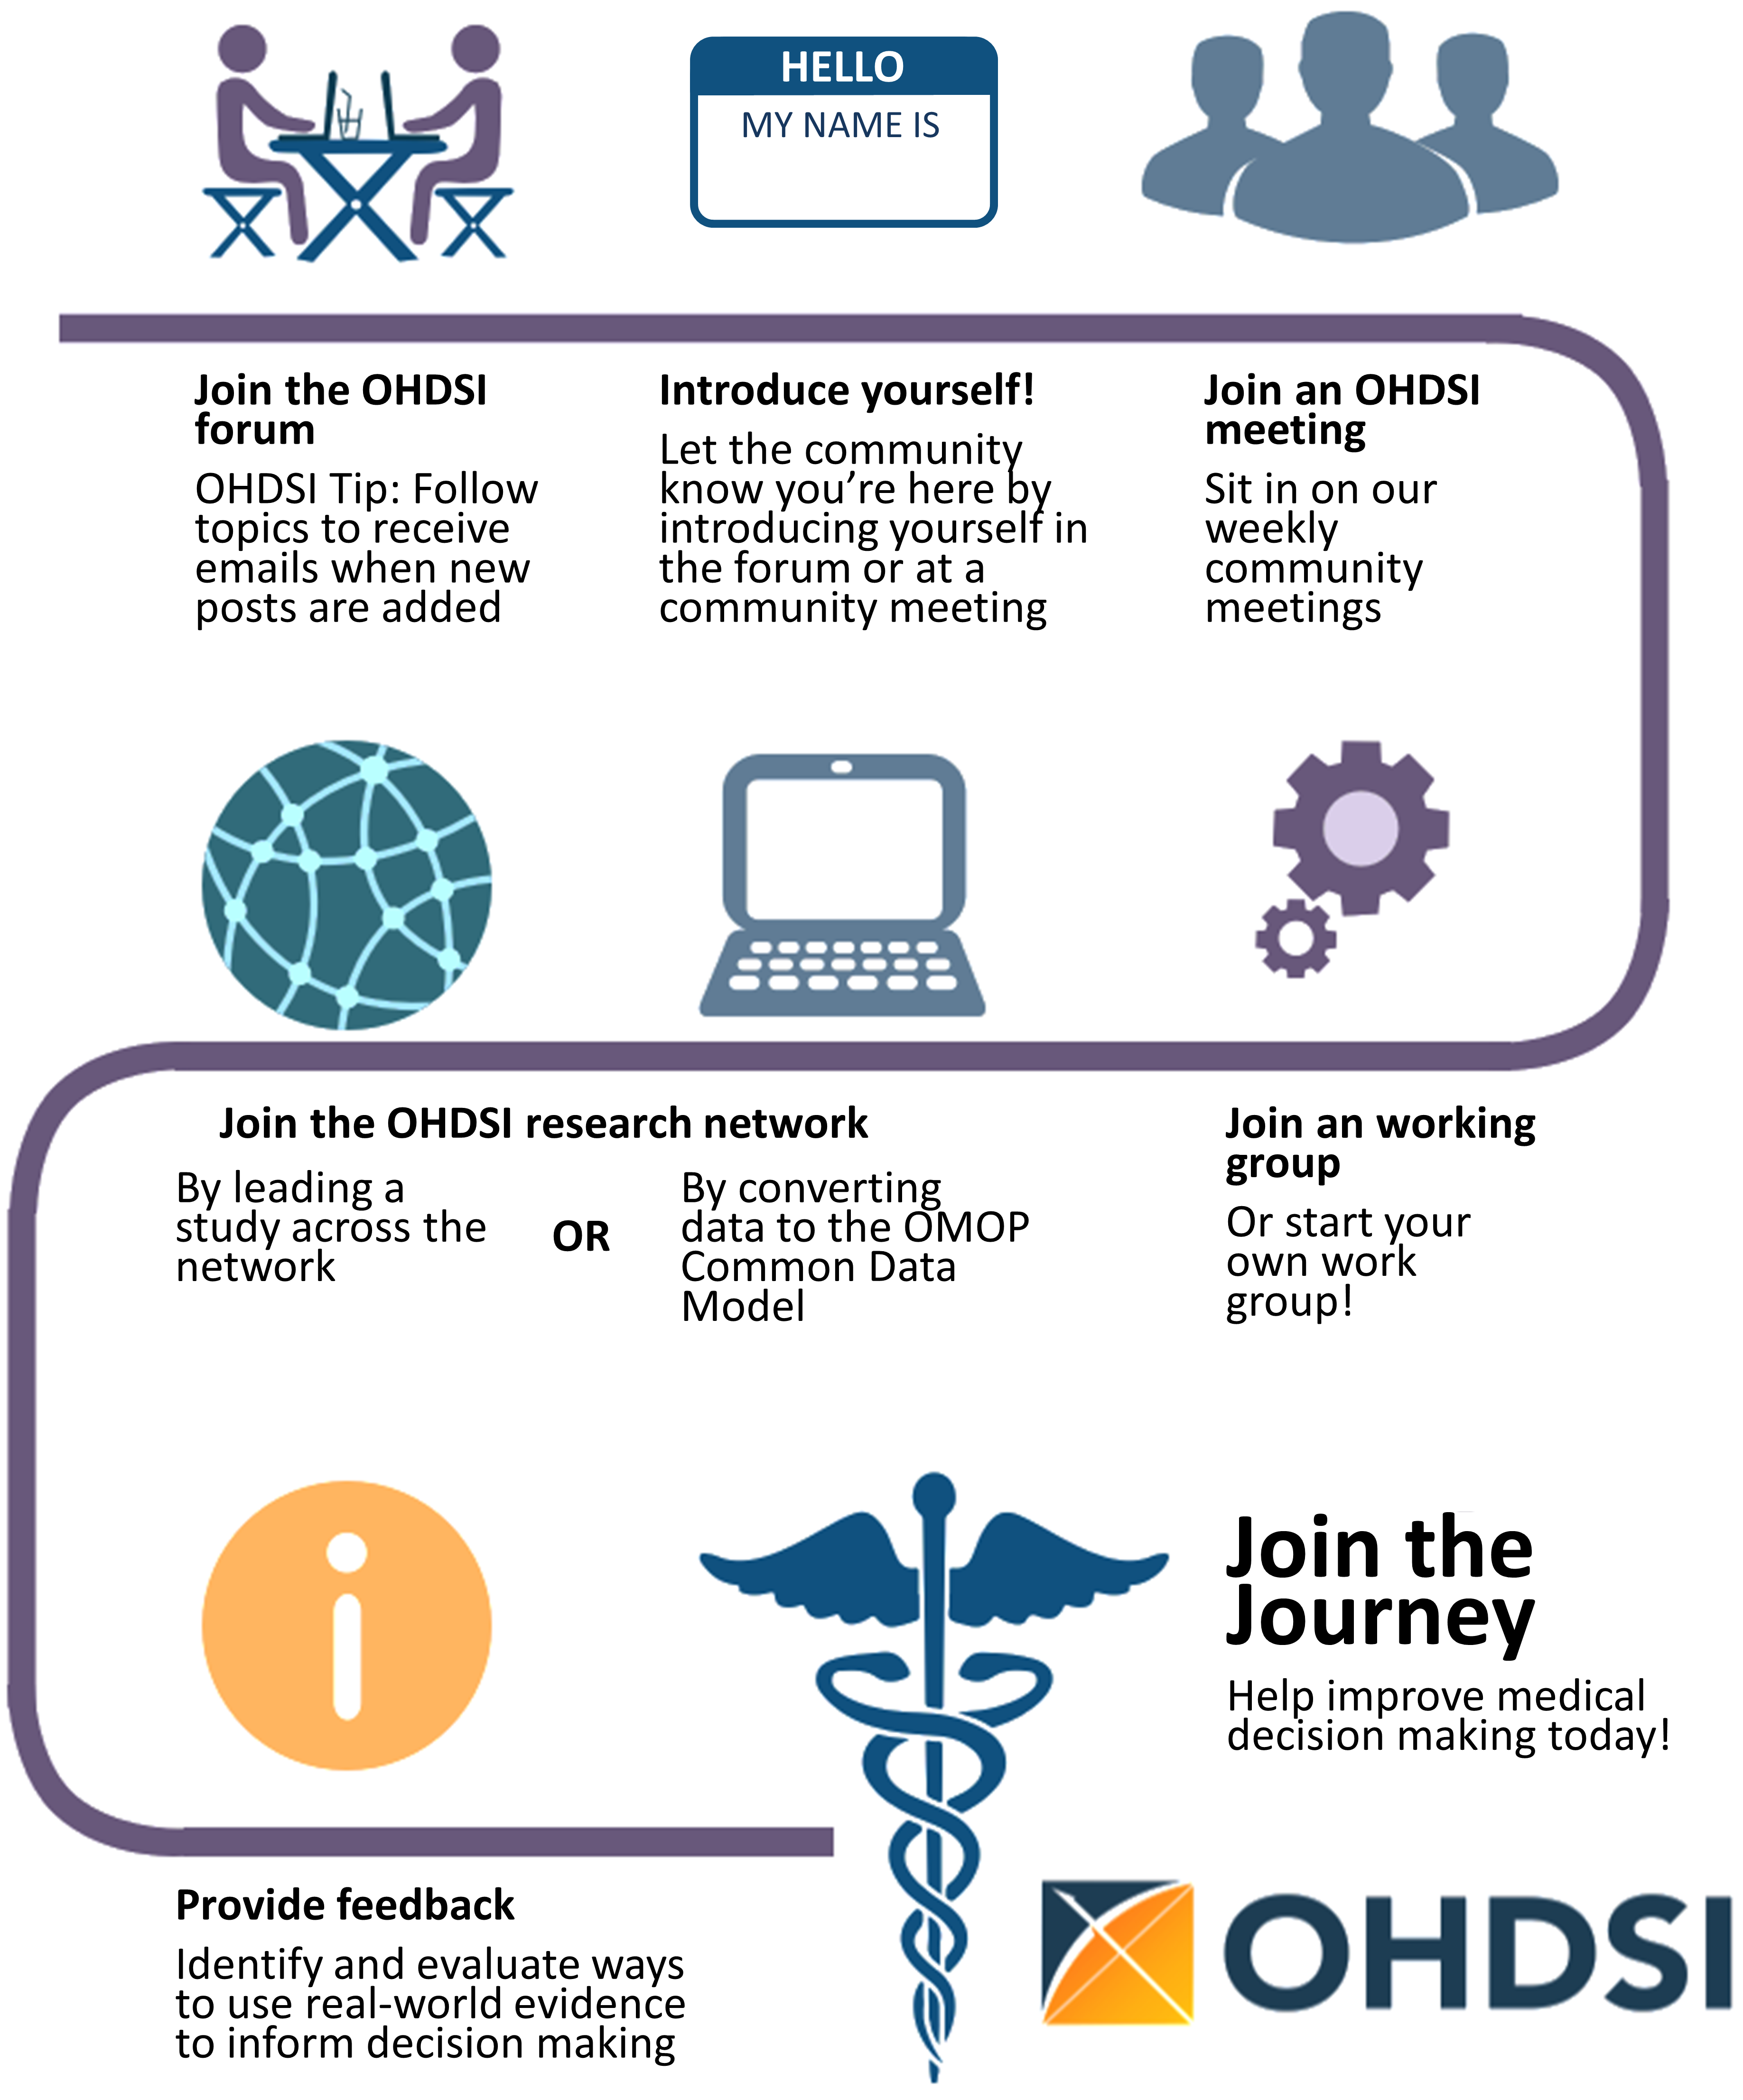
\includegraphics[width=0.9\linewidth]{images/WhereToBegin/joinTheJourney} 

}

\caption{여정에 동참하십시오 - OHDSI의 협력자가 되는 법.}\label{fig:jointhejourney}
\end{figure}

\hypertarget{ohdsi-}{\subsection{OHDSI 포럼}\label{ohdsi-}}

OHDSI 포럼\footnote{\url{http://forum.ohdsi.org}}은 OHDSI 커뮤니티
공동연구자들이 메시지를 올리는 형식을 통해 대화하는 온라인 토론
사이트이다. 포럼은 트리와 같은 구조로 구성되었다. 가장 상위에는
``카테고리''가 있으며 관련성 있는 토론 카테고리로 나눠진다. 각 카테고리
아래로는 하위 포럼과 추가적인 하위 포럼들로 구성된다. 각 토픽
(스레드라고도 불림) 의 가장 낮은 하위 포럼에서 포럼 멤버들 간의 토론
혹은 포스트가 작성된다.

OHDSI 포럼에서는 다음을 포함한 콘텐츠 카테고리를 찾을 수 있다:

\begin{itemize}
\tightlist
\item
  \textbf{일반 General}: OHDSI 커뮤니티와 참여 방법에 대한 전반적인 토론
\item
  \textbf{구현 Implementers}: 로컬 환경에서 공동 데이터 모델과 OHDSI
  분석 프레임워크을 구현하는 방법에 대한 토론
\item
  \textbf{개발자 Developers}: OHDSI 어플리케이션의 오픈 소스 개발과 OMOP
  CDM과의 균형을 위한 도구에 관한 논의
\item
  \textbf{연구자 Researchers}: OHDI 연구 네트워크 기반의 근거 생성, 공동
  연구, 통계적 방법과 기타 CDM 기반 연구에 대한 토론
\item
  \textbf{CDM 개발자 CDM Builders}: 진행 중인 CDM을 위한 조건,
  vocabulary 그리고 테크닉적인 요소들에 관한 토론
\item
  \textbf{Vocabulary 유저 Vocabulary Users}: Vocabulary 콘텐츠에 관한
  토론
\item
  \textbf{지역 지부 Regional Chapters(예를 들면, 한국, 중국, 유럽)}:
  지역별 언어로 진행되며 로컬 OMOP 구현과 OHDSI 커뮤니티 활동에 관한
  토론
\end{itemize}

개별적인 주제로 포스팅을 올리려면 계정 등록을 먼저 해야 한다. 포럼
계정을 오픈하고 나면 General Topic 아래 ``Welcome to OHDSI! -- Please
introduce yourself''라는 토픽에 하기와 같이 본인 소개를 하는 것을
추천한다. 1) 본인 소개 및 본인의 업무 소개 2) 커뮤니티 안에서 어떤
방식으로 도움을 줄 수 있는지 (예를 들면, 소프트웨어 개발, 연구, 논문
작성 등)를 본인 소개에 설명한다. 이제 당신은 OHDSI 여정에 동참하였다!
이후엔 토론에 참여하는 것을 권장한다. OHDSI 커뮤니티 포럼을 통해 자신의
질문을 포스팅하고 새로운 아이디어를 내고, 협업에 참여하길 바란다.
\index{forum}

\BeginKnitrBlock{rmdimportant}
토픽을 ``watch'' 할 수도 있다. 이 뜻은 관심 있는 토픽에 새로운 포스트가
올라올 경우, 이메일로 안내를 받고 이메일 답장을 통해 다시 답장을 보낼
수도 있다는 것이다. 앞으로 다가올 미팅에 대한 아젠다도 확인할 수 있으며
공동작업 기회와 주간 OHDSI 다이제스트를 이메일로 수령할 수 있다.
\EndKnitrBlock{rmdimportant}

\hypertarget{ohdsi-}{\subsection{OHDSI 이벤트}\label{ohdsi-}}

OHDSI는 정기적으로 직접 참여가 가능한 이벤트를 개최하여 공동연구자들이
서로 학습하고 향후 협력 관계를 강화할 기회를 제공한다. 이러한 이벤트는
OHDSI웹사이트를 통해 전달되며 참석에 관심이 있는 사람들에게 무료로
제공된다.

OHDSI 심포지엄은 미국, 유럽, 아시아 등에서 매년 개최되는 과학
컨퍼런스로, 이를 통해 공동 연구자들은 총회, 포스터 발표 및 소프트웨어
시연 등을 통해 각각의 최신 연구를 발표할 수 있다. OHDSI심포지엄은
OHDSI커뮤니티에서 진행되고 있는 최신의 상황을 배울 수 있는 최적의
장소이다. 일반적으로 OHDSI심포지엄에서는 새로운 커뮤니티 참여자들이
데이터 표준이나 분석에 대한 모범사례에 관한 주제들에 대해 배울 수 있는
OHDSI 튜토리얼이 함께 진행된다.

OHDSI공동연구자들의 대면 이벤트 face-to-face event는 좀 더 규모가 작은
포럼인데, 일반적으로 공동으로 관심을 가지고 있는 특정 문제들을 중심으로
구성된다. 지난 이벤트 중에는 표현형 해커톤 phenotype hack-a-thon, 데이터
질 해커톤 data quality hack-a-thon, 오픈소스 소프트웨어
documentation-a-thon 등이 있었다. OHDSI는 다양한 스터디톤 study-a-thon
이벤트를 개최해 왔으며, 이를 통해 공동연구자들이 며칠간 함께 팀이 되어
특정 연구주제에 대하여 적절한 관찰형 분석과 OHDSI 네트워크에 관한 학습,
많은 사람에게 알릴 수 있는 근거를 생성할 수 있는 기회를 제공하였다. 이런
행사들에서는 공통의 문제를 해결하려는 열망뿐 아니라, 배움과 지속적인
발전을 도모하는 우호적 환경을 제공하고자하는 관심도 대두되었다.

OHDSI 커뮤니티의 힘을 보다 자세히 배우기 바란다. OHDSI 웹사이트의
\href{https://www.ohdsi.org/past-events/}{OHDSI Past Events section}에서
지난 심포지엄, 대면 이벤트, OHDSI 튜토리얼 등을 접할 수 있다.

\subsection{OHDSI 커뮤니티 원격회의}\label{ohdsi--}

OHDSI 커뮤니티 주간 원격회의(OHDSI call)는 매주 OHDSI 커뮤니티 안에서
발생하는 활동들에 대해 배울 기회이다. 한국 시각으로 매주 수요일 새벽 2시
(미국 동부시각 기준 화요일 오후 12시부터 1시)에 원격회의로 진행되고
있으며 OHDSI 소프트웨어의 최근 개발 사항 뿐 아니라 개별 공동 연구자들 및
그룹 활동과 커뮤니티의 전체적인 성과를 알 수 있는 기회이다. 이 미팅은
모두 녹화되고 있으며 발표자료들은 OHDSI 웹사이트 리소스에서 확인할 수
있다.

우리는 모든 OHDSI공동 연구자들이 주간 원격회의에 참석하고 커뮤니티
토론을 위한 주제를 제안하기를 바란다. OHDSI 커뮤니티 원격회의는 연구
결과를 공유하고 현재 활발히 진행 중인 작업에 대한 의견을 제시하고
피드백을 얻으며, 개발 중인 오픈소스 소프트웨어를 시연하고, 데이터
모델링과 분석에 대한 모범사례를 커뮤니티와 함께 논의하고,
보조금/간행/컨퍼런스 워크샵 등을 위한 미래의 공동 작업 기회에 대해 많은
아이디어를 논의하는 장이 될 수 있다. 만약 원격회의 발표와 관련한
아이디어가 있다면 OHDSI 포럼에 글을 올릴 수 있다.

OHDSI 신입이라면 원격회의를 통해 OHDSI 네트워크 내에서 일어나는 일들에
대하여 알아가는 것이 좋을 것이다.OHDSI 원격회의에 참여하기 원한다면
\href{https://www.ohdsi.org/web/wiki/doku.php?id=projects:ohdsi_community}{OHDSI
Wiki}를 참고하기 바란다. 커뮤니티 원격회의의 주제는 매주 다르다. OHDSI
포럼의 OHDSI 주간 다이제스트를 통해 매주 발표주제에 관한 정보를 받을 수
있다. 매 원격회의마다 처음으로 참여하는 사람들의 배경과 OHDSI 가입
동기에 관한 소개를 받는 시간을 가진다. \index{community!community calls}

\hypertarget{ohdsi-}{\subsection{OHDSI 워크그룹}\label{ohdsi-}}

OHDSI에는 워크그룹 Workgroup 팀들이 이끌어가는 다양한 프로젝트가 있다.
각각의 워크그룹은 커뮤니티에 기여하기 위한 프로젝트의 목적, 목표,
세부사항 등을 결정하는 리더십을 가지고 있다. 프로젝트 목적과 목표에
기여하고 싶은 참가자라면 누구나 워크그룹에 참여할 수 있다. 워크 그룹은
장기적인 목표을 위해 오랫동안 유지되기도 하고, 커뮤니티의 특정 필요를
충족시키기 위한 단기 프로젝트를 위해 단기적으로만 유지되기도 한다. 워크
그룹의 정기 미팅은 프로젝트 리더들에 의해 결정되며 그룹마다 각각 다르다.
활동 중인 워크 그룹들의 리스트는
\href{https://www.ohdsi.org/web/wiki/doku.php?id=projects:overview}{OHDSI
Wiki}에서 관리되고 있다. \index{workgroups}

테이블 \ref{tab:OHDSIworkgroups}은 활동 중인 OHDSI 워크 그룹의
레퍼런스를 제공한다. 해당 프로젝트에 적극적으로 참여하여 배우길 바란다.

\begin{longtable}[]{@{}lll@{}}
\caption{\label{tab:OHDSIworkgroups} 주목할 만한 OHDSI 워크
그룹}\tabularnewline
\toprule
\begin{minipage}[b]{0.11\columnwidth}\raggedright\strut
Workgroup Name\strut
\end{minipage} & \begin{minipage}[b]{0.44\columnwidth}\raggedright\strut
Objective\strut
\end{minipage} & \begin{minipage}[b]{0.37\columnwidth}\raggedright\strut
Target Audience\strut
\end{minipage}\tabularnewline
\midrule
\endfirsthead
\toprule
\begin{minipage}[b]{0.11\columnwidth}\raggedright\strut
Workgroup Name\strut
\end{minipage} & \begin{minipage}[b]{0.44\columnwidth}\raggedright\strut
Objective\strut
\end{minipage} & \begin{minipage}[b]{0.37\columnwidth}\raggedright\strut
Target Audience\strut
\end{minipage}\tabularnewline
\midrule
\endhead
\begin{minipage}[t]{0.11\columnwidth}\raggedright\strut
Atlas \& WebAPI\strut
\end{minipage} & \begin{minipage}[t]{0.44\columnwidth}\raggedright\strut
Atlas \& WebAPI는 OHDSI 오픈소스 소프트웨어 중 하나로 OMOP-CDM 기반의 한
표준화된 분석 기능을 제공하는 것에 중점을 두고 있다.\strut
\end{minipage} & \begin{minipage}[t]{0.37\columnwidth}\raggedright\strut
오픈소스 Atlas/WebAPI 플랫폼의 개선과 기여하고 싶은 Java와 JavaScript
소프트웨어 개발자들\strut
\end{minipage}\tabularnewline
\begin{minipage}[t]{0.11\columnwidth}\raggedright\strut
CDM \& Vocabulary\strut
\end{minipage} & \begin{minipage}[t]{0.44\columnwidth}\raggedright\strut
임상 환자 빅데이터의 대규모 분석을 위한 체계적이고 표준화된 OMOP-CDM의
지속적인 개발. 타 워크그룹에 의해 개발된 표준화된 분석을 지원하고, 국제
코딩 시스템의 커버리지를 확장하기 위해 표준화된 Vocabulary의 질적
개선.\strut
\end{minipage} & \begin{minipage}[t]{0.37\columnwidth}\raggedright\strut
모든 필요와 사례들에 적용될 OMOP-CDM과 표준 Vocabulary를 개선하고 싶은
사람\strut
\end{minipage}\tabularnewline
\begin{minipage}[t]{0.11\columnwidth}\raggedright\strut
Genomics\strut
\end{minipage} & \begin{minipage}[t]{0.44\columnwidth}\raggedright\strut
다양한 시퀀싱 작업의 결과로 나오는 유전자변이 정보를 위한 Genomic CDM
확장 모델 개발한다.\strut
\end{minipage} & \begin{minipage}[t]{0.37\columnwidth}\raggedright\strut
제한 없음\strut
\end{minipage}\tabularnewline
\begin{minipage}[t]{0.11\columnwidth}\raggedright\strut
Population- Level Estimation\strut
\end{minipage} & \begin{minipage}[t]{0.44\columnwidth}\raggedright\strut
정확하고 믿을 수 있으며 재현 가능한 관찰형 연구의 과학적 방법을 개발하며
이러한 방법의 사용을 촉진한다.\strut
\end{minipage} & \begin{minipage}[t]{0.37\columnwidth}\raggedright\strut
제한 없음\strut
\end{minipage}\tabularnewline
\begin{minipage}[t]{0.11\columnwidth}\raggedright\strut
Natural Language Processing\strut
\end{minipage} & \begin{minipage}[t]{0.44\columnwidth}\raggedright\strut
OHDSI 관찰형 데이터베이스의 문서 데이터 사용을 촉진. 이 목표를 증진하기
위해 OHDSI 연구에 문서 데이터를 활용하기 위한 소프트웨어와 방법을
개발한다.\strut
\end{minipage} & \begin{minipage}[t]{0.37\columnwidth}\raggedright\strut
제한 없음\strut
\end{minipage}\tabularnewline
\begin{minipage}[t]{0.11\columnwidth}\raggedright\strut
Patient- Level Prediction\strut
\end{minipage} & \begin{minipage}[t]{0.44\columnwidth}\raggedright\strut
정확하고 잘 보정된 환자 중심의 표준화된 머신러닝 예측 모델 프로세스를
구축하여 다양한 관심영역에 사용할 수 있게 하며, 또한 어떤 소집단 환자의
데이터에도 적용할 수 있도록 함\strut
\end{minipage} & \begin{minipage}[t]{0.37\columnwidth}\raggedright\strut
제한 없음\strut
\end{minipage}\tabularnewline
\begin{minipage}[t]{0.11\columnwidth}\raggedright\strut
Gold Standard Phenotype Library\strut
\end{minipage} & \begin{minipage}[t]{0.44\columnwidth}\raggedright\strut
OHDSI 참여자들이 함께 검증한 표현형 phenotype 정의와 다른 커뮤니티에서
개발한 표현형 정의를 발견, 평가, 활용하도록 함.\strut
\end{minipage} & \begin{minipage}[t]{0.37\columnwidth}\raggedright\strut
표현형(Phenotype)의 큐레이션과 입증에 관심이 있는 사람\strut
\end{minipage}\tabularnewline
\begin{minipage}[t]{0.11\columnwidth}\raggedright\strut
FHIR Workgroup\strut
\end{minipage} & \begin{minipage}[t]{0.44\columnwidth}\raggedright\strut
OMOP-CDM과 FHIR 통합에 대한 로드맵을 수립하고 OHDSI과 FHIR 상호 간에
서로의 툴과 API를 활용하여 데이터와 연구의 발전을 꾀한다.\strut
\end{minipage} & \begin{minipage}[t]{0.37\columnwidth}\raggedright\strut
상호 운용성(interoperability)에 관심 있는 사람\strut
\end{minipage}\tabularnewline
\begin{minipage}[t]{0.11\columnwidth}\raggedright\strut
GIS\strut
\end{minipage} & \begin{minipage}[t]{0.44\columnwidth}\raggedright\strut
OMOP CDM을 확장하며 OHDSI 툴을 활용하여 환자의 환경 노출 역사가 그들의
임상적 phenotype과 관련이 있게 함.\strut
\end{minipage} & \begin{minipage}[t]{0.37\columnwidth}\raggedright\strut
건강관련 지리적 특성에 관심 있는 사람\strut
\end{minipage}\tabularnewline
\begin{minipage}[t]{0.11\columnwidth}\raggedright\strut
Clinical Trials\strut
\end{minipage} & \begin{minipage}[t]{0.44\columnwidth}\raggedright\strut
OHDSI 플랫폼과 어떤 측면에서도 실험에 도움이 되는 에코시스템의 임상 실험
케이스의 이해 그리고 OHDSI 툴의 업데이트의 도움을 통한 서포트\strut
\end{minipage} & \begin{minipage}[t]{0.37\columnwidth}\raggedright\strut
임상 실험에 관심 있는 사람\strut
\end{minipage}\tabularnewline
\begin{minipage}[t]{0.11\columnwidth}\raggedright\strut
THEMIS\strut
\end{minipage} & \begin{minipage}[t]{0.44\columnwidth}\raggedright\strut
OMOP 사이트에서 디자인 된 ETL 프로토콜들이 높은 퀄리티와 재현할 수
있으며 효율적이도록 확인할 수 있도록 OMOP CDM 규칙에 더하여 표준 규칙의
개발\strut
\end{minipage} & \begin{minipage}[t]{0.37\columnwidth}\raggedright\strut
제한 없음\strut
\end{minipage}\tabularnewline
\begin{minipage}[t]{0.11\columnwidth}\raggedright\strut
Metadata \& Annotations\strut
\end{minipage} & \begin{minipage}[t]{0.44\columnwidth}\raggedright\strut
인간과 기계가 작성한 메타데이터 저장의 표준 프로세스와 공통 데이터
모델의 주석을 정의하여 연구자들이 관찰 데이터 세트의 유용한 데이터
아티팩트를 소비하고 만들어 낼 수 있도록 함.\strut
\end{minipage} & \begin{minipage}[t]{0.37\columnwidth}\raggedright\strut
제한 없음\strut
\end{minipage}\tabularnewline
\begin{minipage}[t]{0.11\columnwidth}\raggedright\strut
Patient Generated Health Data(PGHD)\strut
\end{minipage} & \begin{minipage}[t]{0.44\columnwidth}\raggedright\strut
스마트폰, 앱, 웨어러블 기기를 통해 생성된 PGHD 데이터의 ETL 규칙, 임상
데이터와의 통합, PGHD의 분석 프로세스의 개발\strut
\end{minipage} & \begin{minipage}[t]{0.37\columnwidth}\raggedright\strut
제한 없음\strut
\end{minipage}\tabularnewline
\begin{minipage}[t]{0.11\columnwidth}\raggedright\strut
Women of OHDSI\strut
\end{minipage} & \begin{minipage}[t]{0.44\columnwidth}\raggedright\strut
OHDSI커뮤니티 내부의 여성들이 함께 모여 과학계, 테크놀로지, 엔지니어링,
수학(STEM) 분야에서 여성으로 겪는 도전을 나누기 위한 포럼 제공. 여성들의
입장에서 관점, 우려 사항, 아이디어를 나누며 OHDSI 커뮤니티가 STEM 분야의
여성들을 지원할 수 있을지에 대한 의견 교환 촉진. 궁극적으로 여성들로
하여금 존경받는 분야에서 여성이 리더가 될 수 있도록 장려.\strut
\end{minipage} & \begin{minipage}[t]{0.37\columnwidth}\raggedright\strut
이 목표에 동감하는 사람\strut
\end{minipage}\tabularnewline
\begin{minipage}[t]{0.11\columnwidth}\raggedright\strut
Steering Committee\strut
\end{minipage} & \begin{minipage}[t]{0.44\columnwidth}\raggedright\strut
모든 OHDSI 활동과 이벤트가 발전해나가는 커뮤니티의 필요사항과 부합하도록
확인함으로 OHDSI의 사명과 비전, 가치를 유지함. 또한 미래 방향에 대한
지침을 제공함으로 콜럼비아 대학에 기반을 둔 OHDSI coordination center의
자문그룹 역할을 수행중.\strut
\end{minipage} & \begin{minipage}[t]{0.37\columnwidth}\raggedright\strut
커뮤니티 내부의 리더들\strut
\end{minipage}\tabularnewline
\bottomrule
\end{longtable}

\subsection{OHDSI 지역 지부}\label{ohdsi--}

OHDSI 지역 지부 Regional Chapter 는 각각의 지리적 위치의 특정 문제를
해결하기 위해 로컬 네트워킹 이벤트 및 회의를 개최하고자 하는 지리적
영역에 위치한 OHDSI 공동 작업자 그룹을 대표한다. 현재 OHDSI 지역 지부는
한국\footnote{\url{http://forums.ohdsi.org/c/For-collaborators-wishing-to-communicate-in-Korean}},
유럽\footnote{\url{https://www.ohdsi-europe.org/}}, 중국\footnote{\url{https://ohdsichina.org/}}
등이 있다. 한국 지부 포럼에서는 한국말을 이용하여 질문과 생각을 올릴 수
있다. 만약 본인의 지역에 OHDSI 지역 지부를 셋업하고 싶다면
\href{https://www.ohdsi.org/who-we-are/regional-chapters}{OHDSI
website}에 설명된 OHDSI 지역 지부 프로세스를 따라 진행할 수 있다.
\index{chapters}

\subsection{OHDSI 연구 네트워크}\label{ohdsi--}

다수의 OHDSI 공동연구자들은 자신의 데이터를 OMOP CDM으로 변환하는 것에
관심이 있다. OHDSI 연구 네트워크는 OMOP 호환성을 준수하기 위해
추출-변환-로드(ETL) 프로세스를 거친 관찰형 데이터베이스의 다양하고
글로벌한 커뮤니티를 대표한다. 만약 OHDSI 커뮤니티에서 당신의 여정에
데이터 변환이 포함되어 있다면 OMOP CDM 및 Vocabulary에 대한 튜토리얼,
변환을 지원하는 무료 툴, 특정 도메인 또는 데이터 타입의 유형을 타겟으로
하는 워크 그룹이 있다. OHDSI 공동연구자들은 OHDSI 포럼을 활용하여 CDM
변환 중에 발생하는 문제를 논의하고 해결하는 것을 권장한다.

\section{적합한 위치}\label{-}

\emph{이제 지금쯤이면 과연 나는 OHDSI 커뮤니티의 어디에 어울릴까?} 라는
고민을 할 것이다.

\textbf{나는 연구를 시작하려는 임상 연구자입니다.} 만약 당신이 OHDSI
연구 네트워크를 사용하여 특정 질문에 답하거나, 논문을 제출하려는 임상
연구자라면, 맞게 찾아온 것이다. 우선 OHDSI 포럼의
\href{https://forums.ohdsi.org/c/researchers}{OHDSI Researchers Topic}에
당신의 아이디어를 게시할 수 있다. 이것은 당신과 비슷한 관심사를 가진
연구자와 연결하는데 도움이 된다. OHDSI는 논문출판을 사랑하며 당신의 연구
주제를 데이터 분석 및 논문으로 신속하게 전환할 수 있는 많은 자원을
보유하고 있다. 이에 관한 자세한 내용은 \ref{Characterization}장,
\ref{PopulationLevelEstimation}장, \ref{PatientLevelPrediction}장에서
확인할 수 있다.

\textbf{OHDSI 커뮤니티가 생산하는 정보를 읽고 소비하고 싶습니다.} 당신이
환자, 임상의사 혹은 의료 분야 세부 전문가이든, OHDSI는 건강결과(health
outcome)를 더 잘 이해할 수 있도록 고품질의 근거를 제공하고자 한다.
어쩌면 당신은 코딩해본 지 오래되었을 수도 있고, 프로그래밍을 한 번도
해본 적이 없을 수도 있다. 그래도 당신은 이 커뮤니티의 일환이 될 수 있다.
우리는 당신을 근거 소비자 \emph{evidence consumer} -- OHDSI 연구를
행동으로 옮기는 개인- 라고 부른다. 당신은 OHDSI가 어떤 근거를
만들었거나, 만들고 있는지를 파악하기 위해 정밀하게 선별하고, 아마도
당신과 관련된 질문들을 제안하기를 원할지도 모른다. 이런 당신을 토론에
초대한다. \href{http://forum.ohdsi.org}{OHDSI Forum}에 질문을 올리기
바란다. 커뮤니티 원격회의에 참석하여 최신 연구를 들어보십시오. OHDSI
심포지엄 및 대면 미팅에 참석하여 커뮤니티에 직접 참여하십시오. 당신의
질문은 OHDSI 커뮤니티의 중요한 부분이다. 당신이 어떤 근거를 찾고 있는지
우리가 알 수 있도록 목소리를 높여주십시오!

\textbf{나는 보건의료분야에서 의사결정을 할 수 있는 위치에 있습니다.
나는 데이터 소유자거나 그 소유자를 대표할 수 있습니다. 나는 내 조직에
있어서 OMOP CDM 및 OHDSI 분석 도구의 유용성을 평가하고 있습니다.} 조직의
관리자/리더로서 OHDSI에 관해 들어봤을 수 있으며 OMOP CDM이 어떻게 당신의
경우에 이용될 수 있는지 궁금할 수 있다. 그렇다면,
\href{https://www.ohdsi.org/past-events/}{OHDSI Past Events}의 자료를
통해 연구의 본문을 보는 것으로 시작할 수 있다. 커뮤니티 원격회의에
참여하여 단순히 청취만 할 수도 있다.
\ref{DataAnalyticsUseCases}장(데이터 분석 사용 사례)은 OMOP CDM 및 OHDSI
분석 도구가 사용할 수 있는 연구의 종류를 이해하는 데 도움이 될 것이다.
당신을 위해 OHDSI 커뮤니티가 당신의 여정에 있다. 관심 있는 특정 영역이
있다면 이에 대한 예를 물어보는 것에 두려워하지 마십시오. 전 세계 200개
이상의 조직이 OHDSI 내에서 협력하고 있으며 이 커뮤니티의 가치를 보여주는
데 도움이 되는 성공 사례가 많다.

\textbf{나는 내 기관의 데이터를 ETL 및 변환하여 OMOP CDM으로 변환하고자
하는 데이터베이스 관리자입니다.} 당신의 데이터를 ``OMOP'' 하고자 하는
것은 고귀하고 가치 있는 사업이다. 만약 ETL 프로세스를 막 시작하는
경우에는
\href{https://www.ohdsi-europe.org/images/symposium-2019/tutorials/OHDSI_Vocabulary_CDM_Tutorial.pdf}{OHDSI
Community ETL Tutorial Slides}를 참조하거나 다가오는 OHDSI 심포지엄에
등록하십시오. THEMIS 워크 그룹 원격회이에 참여하거나 OHDSI 포럼에 질문을
올리는 것을 고려해 보십시오. OMOP CDM의 성공적인 구현을 돕는 것에 관심이
많은 커뮤니티에서 풍부한 지식을 찾을 수 있을 것이다. 부끄러워하지
마십시오.

\textbf{나는 OHDSI 툴 스택에 기여를 하고 싶은 생물통계학자 혹은 방법
개발자입니다.} 무엇보다도 OHDSI method 라이브러리에 당신의 전문 지식을
도입하고 이런 방법을 더욱 잘 개발하기 위한 당신의 열정에 감사를 표한다.
우선 인구 수준 추정이나 환자 수준 예측 워크 그룹 원격회의에 참여하여
커뮤니티의 현 우선순위에 대하여 자세히 들어 보기를 추천한다. OHDSI
도구를 사용하면서 각 GitHub Repo에 문제를 제기할 수도 있다. (예를 들면,
SQL 렌더 패키지의 문제일 경우 OHDSI/SqlRender에 대한 GitHub Repo에
문제를 제기하면 된다) 당신의 기여를 환영한다!

\textbf{나는 OHDSI 도구 스택을 보완하는 도구 만드는 것에 관심이 있는
소프트웨어 개발자입니다.} 커뮤니티에 오신 것을 환영한다! OHDSI 임무의
일환으로 우리의 툴은 오픈소스이며 Apache licenses에 따라 관리된다. OHDSI
도구 스택을 보완하는 솔루션 개발을 환영한다. 언제든 워크 그룹에 참여하여
아이디어를 제안해 주길 바란다. 다만, OHDSI는 오픈 사이언스 (개방형 과학)
개방형 협업에 많은 투자를 하는 점을 유의하십시오. 독점적인 알고리즘과
소프트웨어 솔루션도 환영하지만, 그러한 작업은 우리 소프트웨어 개발
작업에서 주요 관심사는 아니다.

\textbf{나는 OHDSI커뮤니티에 조언을 하고 싶은 컨설턴트입니다.}
커뮤니티에 오신 것을 환영한다! 당신의 전문 지식은 매우 귀중하다. 필요에
따라 OHDSI 포럼에 적절히 본인의 서비스를 홍보해도 된다. OHDSI 튜토리얼에
참여하길 바라며 매년 열리는 심포지엄의 절차와 OHDSI 대면 미팅에서 당신의
전문 지식으로 기여하는 것을 고려해 보자.

\textbf{나는 OHDSI에 대하여 더 배우고 싶은 학생입니다.} 올바르게
찾아왔다! OHDSI 커뮤니티 원격회의에 참여하여 본인을 소개하는 것을
고려하십시오. OHDSI 튜토리얼을 참고하고 OHDSI 심포지엄의 대면 미팅에
참여하여 OHDSI 커뮤니티가 제공하는 방법과 툴에 관하여 자세히
알아보십시오. 만약 특정 연구에 관심이 있다면 OHDSI 포럼의 연구자 토픽에
글을 올려보기 바란다. 다양한 조직에서 OHDSI가 후원하는 연구 기회 (예를
들면 박사후과정, 연구 펠로우십) 를 제공한다. OHDSI 포럼은 이러한 기회
등에 대한 최신 정보를 제공할 것이다.

\section{요약}\label{-1}

\BeginKnitrBlock{rmdsummary}
\begin{itemize}
\item
  OHDSI 커뮤니티에서 시작하는 것은 매우 쉽다! \textbf{OHDSI Forum}에
  글을 올리고 원격 회의에 참여하십시오.
\item
  OHDSI 포럼에 본인의 연구나 CDM, ETL질문을 올리기 바란다.
\end{itemize}
\EndKnitrBlock{rmdsummary}

\chapter{오픈 사이언스}\label{OpenScience}

\index{open science}

\emph{Chapter lead: Kees van Bochove}

OHDSI 창립 당시로부터 지금까지 OHDSI 커뮤니티의 목표는 오픈 소스
소프트웨어의 사용이나, 모든 컨퍼런스의 절차 및 자료의 공공적 가용성
그리고 생산된 의학적 근거의 투명한 공개 접근과 같이 오픈 사이언스의
가치를 구축함으로써 국제 적 협력체계를 구축하는 것이었다. 그러나, 오픈
소스 소프트웨어란 정확히 무엇을 말하는가? 그리고 OHDSI가 어떻게 개인
정보보호에 매우 민감하고, 통상적으로 선한 의도만으로는 구할 수 없는 의료
데이터에 대한 개방형 데이터 전략이나 오픈 사이언스 전략을 구축할 수
있었을까? 왜 분석의 재현성을 갖는 것이 그렇게 중요할까? 그리고 OHDSI
커뮤니티는 어떻게 이 목표를 달성하고자 하는가? 이는 우리가 이 장에서
다룰 문제들 중 몇가지이다.

\section{오픈 사이언스}\label{-}

`오픈 사이언스(Open Science)'라는 용어는 90년대부터 사용되어 왔다.
하지만 OHDSI가 생겨난 2010년대부터 견인력을 얻기 시작했다. 위키피디아
\citep{wiki:Open_science} 는 이 용어의 뜻을 ``과학 연구 (간행물, 데이터,
실제 샘플 및 소프트웨어 포함) 를 만들어내고 사회, 아마추어 또는 전문가의
모든 수준에서의 접근을 전파하는 운동''이라 정의하고 있으며 더 나아가
일반적으로 공동 네트워크를 통해 개발된다고 말한다. OHDSI 커뮤니티는
자체적으로 '오픈 사이언스' 집단 혹은 네트워크라고 정의하지 않았으나 이
용어는 OHDSI의 개념과 원칙을 사용하는데 자주 사용된다. 예를 들어 2015년
Jon Duke는 OHDSI를 ``의료 근거 생성에 관한 오픈 사이언스
접근법''\footnote{\url{https://www.ohdsi.org/wp-content/uploads/2014/07/ARM-OHDSI_Duke.pdf}}
이라 말하였으며 2019년에는 EHDEN 컨소시움의 입문용 웹 세미나에서는 OHDSI
네트워크 접근 방식을 ``21세기 실세계 오픈 사이언스''\footnote{\url{https://www.ehden.eu/webinars/}}
라고 극찬하였다. 이번 장에서 보게 되겠으나 오픈 사이언스의 많은 실행들은
오늘날의 OHDSI 커뮤니티에서 발견될 수 있다. 어떤 이들은 OHDSI 커뮤니티는
의료 근거 생성의 투명성과 신뢰성을 개선하기 위한 공동 욕구에 의해 시작된
풀뿌리 오픈 사이언스 집단이라고 주장하기도 한다.

오픈 사이언스 또는 ``사이언스 2.0'' \citep{wiki:Science_2.0} 접근법은
현재 의학계의 관행에서 인식된 여러가지 문제를 해결할 것이다. 정보 기술은
데이터 생성 및 분석 방법의 폭발적인 증가로 이어졌으며 개별 연구원의 경우
전문 분야에 발표된 모든 문헌을 따라잡기가 매우 어렵다. 특히 평소
진료일을 하면서 최신 의학에 뒤처지지 않아야 하는 임상 의사의 경우는 훨씬
더 그렇다. 게다가, 많은 수의 실험들이 열악한 통계 디자인, 편향된 발행물,
p-hacking 및 유사한 통계적 문제로 영향을 받고 있으며 재현하기 어렵다는
우려가 커지고 있다. 이러한 우려를 교정하기 위한 전통적인 방법인 출간된
논문에 대한 Peer review로는 이런 문제들을 찾아서 해결하지 못한다. 2018년
Nature의 특집호에서 ``재현할 수 없는 연구의 어려움''\footnote{\url{https://www.nature.com/collections/prbfkwmwvz}}은
몇가지 예를 보여주었다. 한 저자 그룹은 자신들이 속한 분야의 논문들에서
체계적 문헌고찰을 적용하려 하였으나, 여러가지 이유로, 식별된 논문 오류를
수정하기 어렵다는 것을 발견하였다. 특히 결함이 있는 디자인으로 시작한
실험은 특히 수정하기 어렵다. Ronald Fisher의 말에 의하면 ``실험을 마친
후 통계학자와 상담하는 것은 마치 그에게 사체부검을 해달라는 것과 같다.
아마 무엇 때문에 그 실험이 사망했는지는 말해줄 수 있겠지요.''
\citep{wikiquote:Ronald_Fisher} 저자는 통계적 의미나 메타분석의 잘못된
계산, 부적절한 기준선 비교와 관련된 잘못된 결론을 이끌게 되는 결함 있는
무작위 실험설계 같은 통계적 문제들을 흔히 만난다. \citep{allison_2016}
물리학의 경험을 예로 들면, 같은 컬렉션의 또 다른 논문에서는, 기본
데이터를 이용할수 있게 제공할 뿐 아니라, 데이터 처리와 분석 사본을
출판하고 적절한 기록 문서로 만들어서 충분히 재현해볼 수 있도록 하는 것이
중요하다고 주장한다. \citep{Chen2018}

OHDSI 커뮤니티는 이러한 어려움들에 대해 자체적으로 해결하고, 대규모로
의학 근거를 만드는 것이 중요하다는 데 중점을 두고 있다. Schuemie와 Ryan
등이 \citet{schuemie_2018b} 에서 언급하였듯이 현 패러다임은 ``알 수 없는
신뢰성과 한 번에 하나의 추정치를 출판할 수 있는 고유한 실험 설계를
통하여 한 번에 하나의 추정치를 생성하는데 중점을 두고''있으나 OHDSI
커뮤니티는 일관되고 표준화된 방법을 사용하여 대규모 처리를 통한 관찰
연구를 지지하며, 평가, 교정 및 편견 없는 결과발표를 통해 보다 안정적이고
완전한 근거 기반을 만들 수 있다. 이는 데이터를 OMOP CDM에 매핑하는 의료
데이터 소스 네트워크와, 모든 사람들이 사용할수 있고 증명할수 있는 오픈
소스 분석 코드, 그리고, howoftten.org에서 발표한 질환 발생 관련한 대규모
기준 데이터들을 조합하여 이룰 수 있다. 다음 단락에서는 구체적인 예시를
보여주고, 공개 표준, 오픈 소스, 공개 데이터, 열린 담론의 4가지 원칙을
이용하여 OHDSI의 오픈 사이언스 접근 방식을 보다 자세히 설명할 것이다.
이번 장에서는 오픈 사이언스의 관점에서 OHDSI 에 대한 공정한 원칙과
전망에 대해 간략하게 참고한 것으로 마무리 한다.

\section{실천의 오픈 사이언스: Study-a-Thon}\label{---study-a-thon}

\index{study-a-thon}

커뮤니티 내부의 최근 동향은 `Study-a-thons'의 출현이다. Study-a-thon이란
OMOP 데이터 모델과 OHDSI 툴을 사용하여, 중요하고 임상적으로 관련이 있는
연구 질문에 대답하기 위해 여러 학문 분야에 걸친 과학자들이 모여서 짧고
집중된 대면회의를 하는 모임이다. 이에 관한 좋은 예는 EHDEN 웨비나 에서
설명한 2018 Oxford study-a-thon 인데, 과정을 단계별로 제공하고
공개적으로 사용할 수 있는 결과를 강조하고 있다. Study-a-thon에 이어지는
기간 동안, 참가자는 의학적으로 관련이 있는 연구 주제를 제안하고 하나
이상의 연구 주제는 study-a-thon 자체가 진행되는 동안 연구될 수 있도록
선정된다. OMOP 형식의 환자 레벨 데이터에 접근할 수 있고 이러한 데이터
소스에 추출 조건을 만들어 수행할 수 있는 참가자들을 통해 데이터가
제공된다. 실제 study-a-thon 시간의 대부분은 통계적 접근법
(\ref{WhereToBegin}장 참조), 데이터 소스의 적합성, 상호작용으로 만들어진
결과와 이러한 결과에 의해 필연적으로 제기되는 후속 질문에 대해
논의하는데 사용된다. Oxford study-a-thon의 경우 다양한 무릎 대체 수술 후
발생하는 부작용에 대한 연구를 중심으로 질문이 이루어졌으며 OHDSI 포럼 및
tool 을 이용하여 study-a-thon이 진행하는 동안 대화식으로 결과를
발표하였다. (\ref{OhdsiAnalyticsTools}장 참조) ATLAS와 같은 OHDSI tool은
코호트 정의의 신속한 생성, 교환, 토론 및 평가를 용이하게 하여, 문제
정의와 방법 선택에 대한 합의에 도달하는 초기 프로세스를 아주 빠르게
가속화 해준다. 관련 데이터 소스와 OHDSI 오픈소스 환자 수준 예측(patient
level prediction) 패키지 \ref{PatientLevelPrediction}의 사용성 덕분에,
하루만에 수술 후 90일 사망률에 대한 예측 모델을 만들고, 다음 날 여러
대규모 데이터 소스에서 이 모델에 대한 외부 검증이 가능했다. 또한
study-a-thon은 전통적인 학술 논문 (무릎 관절 전체 성형술 부작용에 대한
patient-level의 예측 모델의 개발 및 검증, Ross Williams, Daniel
Prieto-Alhambra et al., 논문 작성 중) 을 만들어 냈는데, Peer review를
통해서 진행되었다면 몇 달 걸렸을 작업이다. 그러나 수억 명의 환자 기록을
다루는 다수의 의료 데이터베이스에 대한 분석 스크립트와 결과가 1주일 안에
낙서 같은 초안으로부터 설계, 생산 및 출판되었다는 사실은 OHDSI 가 근거를
만드는데 필요한 처리 기간을 몇달에서 몇일로 감소시켜서 의학 분야를
근본적으로 향상시킬 수 있다는 것을 보여 준다.

\section{공개 표준}\label{-}

\index{open science!open standards}

OHDSI 커뮤니티에서 유지 관리되는 매우 중요한 커뮤니티 리소스는 OMOP 공통
데이터 모델 (\ref{CommonDataModel}장 참조) 와 관련 표준용어
(\ref{StandardizedVocabularies}장 참조) 이다. 모델 자체는 관찰 의료
데이터를 수집하기 위해 범위가 정해졌으며 원래는 약물, 시술, 의료기기
등에 노출되는 것과 진단 및 검사와 같은 결과 간의 연관성을 분석하기 위한
것이었으나 이제는 다양한 분석 사용 사례로 확장되었다.
(\ref{DataAnalyticsUseCases}장 참조) 그러나 다양한 코딩 시스템, 의료
패러다임 및 다양한 유형의 의료 소스를 가진 전 세계의 의료 데이터를
통일시키려면 소스 코드와 가장 가까운 표준화된 용어 간에 엄청난 양의
'매핑'이 필요하다. OMOP 표준용어는 \ref{DataAnalyticsUseCases}장에서
추가로 설명한다. OMOP 표준용어는 전 세계적으로 사용되는 수백 개의 의료
코딩 시스템과의 매핑을 포함하고 있으며 OHDSI Athena 툴을 통해 열람할 수
있다. 이러한 vocabulary와 매핑을 자유롭게 사용할 수 있는 리소스로
커뮤니티에 제공함로써, OMOP과 OHDSI커뮤니티는 의료 데이터 분석에 상당한
기여를 하고 있으며, 몇 몇 연구자에 의하면, 이러한 목적을 위한 가장
포괄적인 모델이며 전세계적으로 약 12억 명의 의료 기록을 대표하고
있다.\footnote{\url{https://www.ema.europa.eu/en/events/common-data-model-europe-why-which-how}}
\citep{garza_2016} - (역자 주: 최근 조사자료에 의하면 약 21억명, 미국을
제외시 약 3억 8천만명 자료. 기관간 자료가 연계되지 않으므로 한 환자의
자료가 어려번 중복됨으로 인해서 포함된 실제 고유 환자 수에 비해서 더
많게 평가됨)

\section{오픈 소스}\label{-}

\index{open science!open source}

OHDSI 커뮤니티가 제공하는 또 다른 핵심 리소스는 오픈 소스 프로그램이다.
여기에는 데이터를 OMOP에 매핑하기 위한 도우미 툴
(\ref{ExtractTransformLoad}장 참조), 일반적으로 사용되는 강력한 통계
방법을 포함하는 OHDSI 메소드 라이브러리, 공개된 관찰 연구를 위한 오픈
소스 코드, OHDSI ecosystem을 뒷받침하는 ATLAS, Athena 및 기타 인프라
관련 소프트웨어 (\ref{OhdsiAnalyticsTools}장 참조) 로 나눌 수 있다. 오픈
사이언스 관점에서, 가장 중요한 리소스 중 하나는 OHDSI연구 네트워크와
같은 실제 연구 실행을 위한 코드이다. (\ref{NetworkResearch}장 참조) 그
다음에, 이 프로그램들은 GitHub를 통해 점검, 검토 및 기여가 가능한 완전
오픈 소스 OHDSI 스택을 활용한다. 예를 들어, 네트워크 연구는 분석법 이용
사례에 대한 통계적 방법을 일관되게 재사용 할 수 있는 라이브러리를
기반으로 하는 경우가 많다. OHDSI의 오픈 소스 소프트웨어 사용과 협력이
생성된 근거들에 대한 품질과 신뢰성을 어떻게 뒷받침하는지에 대해 자세한
개요는 \ref{SoftwareValidity}장을 참고 하기 바란다.

\section{공개 데이터}\label{-}

\index{open science!open data}

개인 정보 보호에 민감한 의료 데이터의 특성 때문에 완전 개방적이고
포괄적인 patient-level데이터 세트는 일반적으로 사용할 수 없다. 그러나
앞서 언급된 \url{http://howoften.org} 및 \url{http://data.ohdsi.org} 에
게시된 다른 공개 결과 세트들과 같은 중요한 집계 데이터나 결과 세트를
게시하기 위해 OMOP 매핑된 데이터 세트를 활용하는 건 가능하다. 또한,
OHDSI 커뮤니티는 테스트와 개발을 위해 SynPUF와 같은 시뮬레이션 데이터
세트를 제공하며, OMOP에 매핑되어서 이용 가능한 데이터 소스들의 네트워크
안에서 연구를 수행하는 데 OHDSI 연구 네트워크 (\ref{NetworkResearch}장
참조) 가 이용될 수 있다. 소스 데이터와 OMOP CDM 간의 매핑을 투명하기
하기 위해 한 매핑을 위해, 데이터 소스가 OHDSI ETL 또는 `매핑' 툴을
재사용하고 매핑 코드를 오픈 소스로도 게시하는 것이 바람직하다. 또한
OHDSI 커뮤니티는 테스트 및 개발 목적으로 SynPUF와 같은 시뮬레이션 된
데이터 세트를 제공하며 OHDSI 리서치 네트워크를 활용하여 데이터를 OMOP에
매핑 한 사용 가능한 데이터 소스 네트워크에서 연구를 실행할 수 있다. 소스
데이터와 OMOP CDM 간의 매핑을 명료하게 하기 위해 OHDSI ETL 또는
'매핑'도구를 재사용하는 동시에 매핑 코드를 공개소스로 게시하는 것이
좋다.

\section{열린 담론}\label{-}

\index{open science!open discourse}

공개 표준, 공개 소스, 공개 데이터는 훌륭한 자산이지만, 그 자체로는 진료
행위에 큰 영향은 없을 것이다. OHDSI의 오픈 사이언스 활동과 영향의 핵심은
의학적 근거 생성을 구현하여 과학으로부터 진료 현장으로 이행하도록 해주는
것이다. OHDSI 커뮤니티는 미국, 유럽, 아시아에서 개최되는 여러 연례 OHDSI
심포지엄을 비롯하여 특히 중국과 한국의 헌신적으로 실천하는 커뮤니티들을
보유하고 있다. 이들 심포지엄에서는 통계적 방법, 데이터 및 소프트웨어 툴
사용법, 표준 용어, 그리고 OHDSI 오픈 소스 커뮤니티의 다른 모든
측면에서의 발전에 대해 논의한다. OHDSI 포럼\footnote{\url{https://forums.ohdsi.org}}과
위키\footnote{\url{https://www.ohdsi.org/web/wiki}}는 전 세계 수천 명의
연구자가 관찰 연구를 수행하도록 돕는다. 커뮤니티 원격회의\footnote{\url{https://www.ohdsi.org/web/wiki/doku.php?id=projects:overview}}와
GitHub\footnote{\url{https://github.com/ohdsi}}의 코드, 이슈, pull
requests는 코드, CDM과 같은 오픈 커뮤니티의 자산을 지속해서 발전시키고
OHDSI 네트워크 연구에서는 전 세계적으로 수억 개의 환자 기록을 이용하여
개방적이고 투명한 방법으로 범세계적 관찰 연구가 수행되고 있다. 개방성과
열린 담론은 커뮤니티 전반에 걸쳐 권장되며 바로 이 책은 OHDSI 위키,
커뮤니티 원격회의, GitHub repository에 의해 촉진되는 오픈 프로세스를
통해 쓰인다. \footnote{\url{https://github.com/OHDSI/TheBookOfOhdsi}}
그러나 OHDSI 공동연구자들이 없다면 프로세스와 도구는 빈 껍데기가 될
것이라는 점을 강조할 필요가 있다. 실제로 OHDSI 커뮤니티의 진정한 가치는
\ref{OhdsiCommunity}장에서 논의한 바와 같이 협력과 오픈 사이언스를 통해
건강을 증진한다는 비전을 공유하는 회원들과 함께한다고 말할 수 있다.

\section{OHDSI와 FAIR의 가이드 원칙}\label{ohdsi-fair--}

\index{FAIR}

\subsection{도입}

이 장의 마지막 단락은 \citet{wilkinson2016} 이 발표한 FAIR 데이터 가이드
원칙을 사용하여 OHDSI 커뮤니티와 도구의 현재 상태를 살펴본다.

\subsection{\texorpdfstring{검색성\\
}{검색성 }}

OMOP에 매핑되어 분석에 사용되는 모든 의료 데이터베이스는 과학적 관점에서
미래 참조와 재현성을 위해 지속하여야 한다. OMOP 데이터베이스를 위한 영구
식별자를 사용하는 것이 아직 널리 확산되지는 않았는데, 부분적으로는
이러한 데이터베이스가 방화벽 뒤에 담겨있거나 내부 네트워크에 있어서,
그리고 인터넷에 반드시 연결되지는 않기 때문이다. 그러나, 인용 목적과
같이 참조할 수 있는 설명 기록으로 데이터베이스 요약을 게시하는 것은
전적으로 가능하다. 이 방법은 EMIF 카탈로그11의 예를 따르며 이 카탈로그는
데이터 수집 목적, 소스, vocabulary 및 용어, 액세스 제어 메커니즘,
라이센스, 동의 등의 측면에서 데이터베이스에 대한 포괄적인 기록을
제공한다. \citep{Oliveira2019} 이 접근 방식은 IMI EHDEN 프로젝트에서
더욱 심층 개발되었다.

\subsection{접근성}

오픈 프로토콜을 통해 OMOP에 매핑된 데이터는 일반적으로 SQL 인터페이스를
통해 이뤄지는데, 이 인터페이스는 OMOP CDM과 결합하여 OMOP 데이터에
접근하기 위한 표준화되고 잘 문서화된 방법을 제공한다. 그러나, 위에서
논의한 바와 같이, OMOP 소스는 보안상의 이유로 인터넷을 통해 직접 이용할
수 없는 경우가 많다. IMI EHDEN과 같은 프로젝트의 활발한 연구 주제와 운영
목표는 연구원들이 접근할 수 있는 안전한 전 세계 의료 데이터 네트워크를
만드는 것이다. 그러나, LEGEND와 \url{http://howoften.org} 과 같은 OHDSI
이니셔티브를 통해 보이듯, 다수의 OMOP 데이터베이스의 분석 결과를
공개적으로 게시될 수 있다.

\subsection{상호운용성}

상호운용성(Interoperability)은 틀림없이 OMOP 데이터 모델과 OHDSI
도구들의 강력한 장점이다. 근거 생성을 위해 활용할 수 있는 전 세계적으로
강력한 의료 데이터 소스 네트워크를 구축하기 위해서는 의료 데이터 소스
간의 상호운용성을 달성하는 것이 핵심이며, 이는 OMOP 모델과
표준용어집(Standardized Vocabularies)을 통해 달성된다. 그러나 코호트
정의와 통계적 접근법을 공유함으로써 OHDSI 커뮤니티는 코드 매핑을 넘어
의료 데이터에 대한 분석 방법의 상호운용 가능한 이해를 만들기 위한
플랫폼을 제공한다. 병원과 같은 의료 시스템은 종종 OMOP 데이터에 대한
기록의 소스이기 때문에, OHDSI 접근방식의 상호운용성은 HL7 FHIR, HL7 CIMI
및 OpenEHR과 같은 운영적인 의료 상호운용성 표준과 일치함으로써 더욱
향상될 수 있다. CDISC나 생물의학 온톨로지 같은 임상적 상호운용성
표준과의 정렬도 마찬가지다. 특히 종양학과 같은 분야에서 이것은 중요한
주제로서, OHDSI 커뮤니티의 Oncology Working Group과 Clinical Trials
Working Group은 이러한 문제가 적극적으로 논의되는 포럼의 좋은 예를
보여준다. 다른 데이터의 참조 및 특히 온톨로지 용어 측면에서, ATLAS와
OHDSI Athena는 다른 이용 가능한 의료 코딩 시스템의 맥락에서 OMOP
표준용어집을 탐색할 수 있기 때문에 중요한 도구이다.

\subsection{재사용 가능성}\label{-}

재사용 가능성(Reusability)에 관한 FAIR 원칙은 데이터 라이센스, 출처
(데이터가 어떻게 존재했는지 명확화) 및 관련 커뮤니티 표준과의 연결과
같은 중요한 문제에 초점을 맞추고 있다. 데이터 라이센스는 복잡한
주제로서, 특히 관할 구역에서 더욱 복잡하며, 광범위하게 다루기에는 이
책의 범위를 벗어난다. 그러나 당신의 데이터 (예를 들면, 분석 결과) 를
다른 사용자가 자유롭게 사용할 수 있도록 하려는 경우 데이터 라이센스를
통해 이러한 권한을 명시적으로 제공하는 것이 좋다. 그러나 아직 인터넷에서
찾을 수 있는 대부분의 데이터에 대한 일반적인 관행이 아니며 불행히도
OHDSI 커뮤니티 역시 예외가 아니다. OMOP 데이터베이스의 데이터 출처와
관련하여, CDM 버전, 표준용어집 배포, 사용자 정의 코드 목록 등과 같이
자동화된 방식으로 메타 데이터를 사용할 수 있도록 하기 위해 잠재적으로
개선할 점이 존재한다. OHDSI ETL 툴은 현재 이 정보를 자동으로 생성하지
않지만, Data Quality Working Group과 Metadata Working Group 같은 워크
그룹은 이에 대해 활발하게 작업 중이다. 또 다른 중요한 측면은 기본
데이터베이스 자체의 출처 검증이다. 병원이나 일반의용 정보시스템이
교체되었는지 또는 변경되었는지, 그리고 알려진 데이터 누락이나 다른
데이터 문제가 과거에 언제 발생했는지를 아는 것이 중요하다. OMOP CDM에서
이러한 메타데이터를 체계적으로 연결하는 방법을 탐색하는 것이 Metadata
Working Group의 영역이다.

\BeginKnitrBlock{rmdsummary}
\begin{itemize}
\item
  OHDSI 커뮤니티는 의료 근거 생성의 상호 운용성과 재현성을 적극적으로
  추구하는 오픈 사이언스 커뮤니티로 볼 수 있다.
\item
  기존의 단일 연구 및 단일 추정 의학 연구 패러다임에서, 실세계 의료
  자료를 이용하여 기초 발생율과 같은 사실을 알리고 중재 및 치료의 효과를
  통계적으로 추정하는 근거를 대규모 및 체계적으로 생성하는
  패러다임으로의 전환을 지지하고 있다.
\end{itemize}
\EndKnitrBlock{rmdsummary}

\part{Uniform Data
Representation}\label{part-uniform-data-representation}

\chapter{공통 데이터 모델}\label{CommonDataModel}

\emph{Chapter leads: Clair Blacketer}

관찰 데이터는 환자가 진료를 받는 동안 어떤 일들이 일어나는지를 보여준다.
전 세계적으로 점점 더 많은 수의 환자에 대한 데이터가 빅 데이터라고
불리는 형태로 수집 및 저장되고 있다. 이러한 수집의 목적은 다음과 같은 세
가지로 설명할 수 있다. (i) 직접적으로 (많은 경우에 설문 조사 및
레지스트리 정보를 활용한) 연구를 용이하게 하기 위해, (ii) 의료 행위
수행을 지원하기 위해 (이를 보통 전자 의무 기록(Electronic Health
Records, EHR)이라고 함), 또는 (iii) 의료비 지불 관리를 위함 (청구
데이터). 세 가지 목적 모두 임상 연구에 보편적으로 사용되나, 두 번째 세
번째 항목은 이차적인 목적으로 사용된다. 위 세가지 모두 일반적으로 고유한
내용의 형식 및 인코딩으로 이루어져 있다. \index{Common Data Model}
\index{CDM |see {Common Data Model}}
\index{relational data model|see {Common Data Model}}

관찰형 의료 데이터(Observational healthcare data)에 공통 데이터 모델이
필요한 이유는 무엇일까?

일차적인 목적에 의해 모든 임상적인 사건들을 동일하게 포착하는 관찰형
데이터베이스(Observational database)는 없다. 따라서, 여러 다른 데이터
출처에서 연구 결과를 도출하고 데이터를 포착하는 과정에서 발생하는 잠재적
비뚤림(bias)의 영향을 이해하기 위해 이를 비교 및 대조해야 한다. 또한
통계적 검증력을 갖춘 결론을 도출하려면 많은 수의 관찰 환자가 필요하다.
이는 여러 데이터 출처를 동시에 평가하고 분석해야 할 필요성을 설명한다.
그러기 위해서는 데이터를 공통 데이터 표준(common data standard)으로
화합할 필요가 있다. 게다가 환자 데이터는 높은 수준의 보안이 필요하다.
기존에 그래왔듯이 분석을 목적으로 하는 데이터 추출은 엄격한 데이터 사용
계약 및 복잡한 접근 제어 방식이 필요하다. 공통 데이터 표준은 추출 단계를
생략하고 기본 환경의 데이터에 대해 표준화된 분석을 실행할 수 있도록 하여
이러한 필요성을 줄여 줄 수 있다 - 분석환경으로 데이터가 오는게 아니고
데이터가 있는 장소로 분석환경이 오는 것.

이러한 표준은 공통 데이터 모델(Common Data Model, CDM)에 의해 제공된다.
CDM은 표준화된 내용을 기반으로 (\ref{StandardizedVocabularies}장 참조)
연구 방법들이 효과적으로 비교 가능하고 재현 가능한 결과를 얻을 수 있게
체계적으로 활용되게 한다. 이 장에서는 데이터 모델을 비롯한 디자인, 규칙
및 테이블 선택에 대한 논의를 제공하고자 한다.

CDM내의 모든 테이블에 대한 개요는 그림 \ref{fig:cdmDiagram}
\index{Common Data Model!data model diagram}에서 살펴볼 수 있다.

\begin{figure}
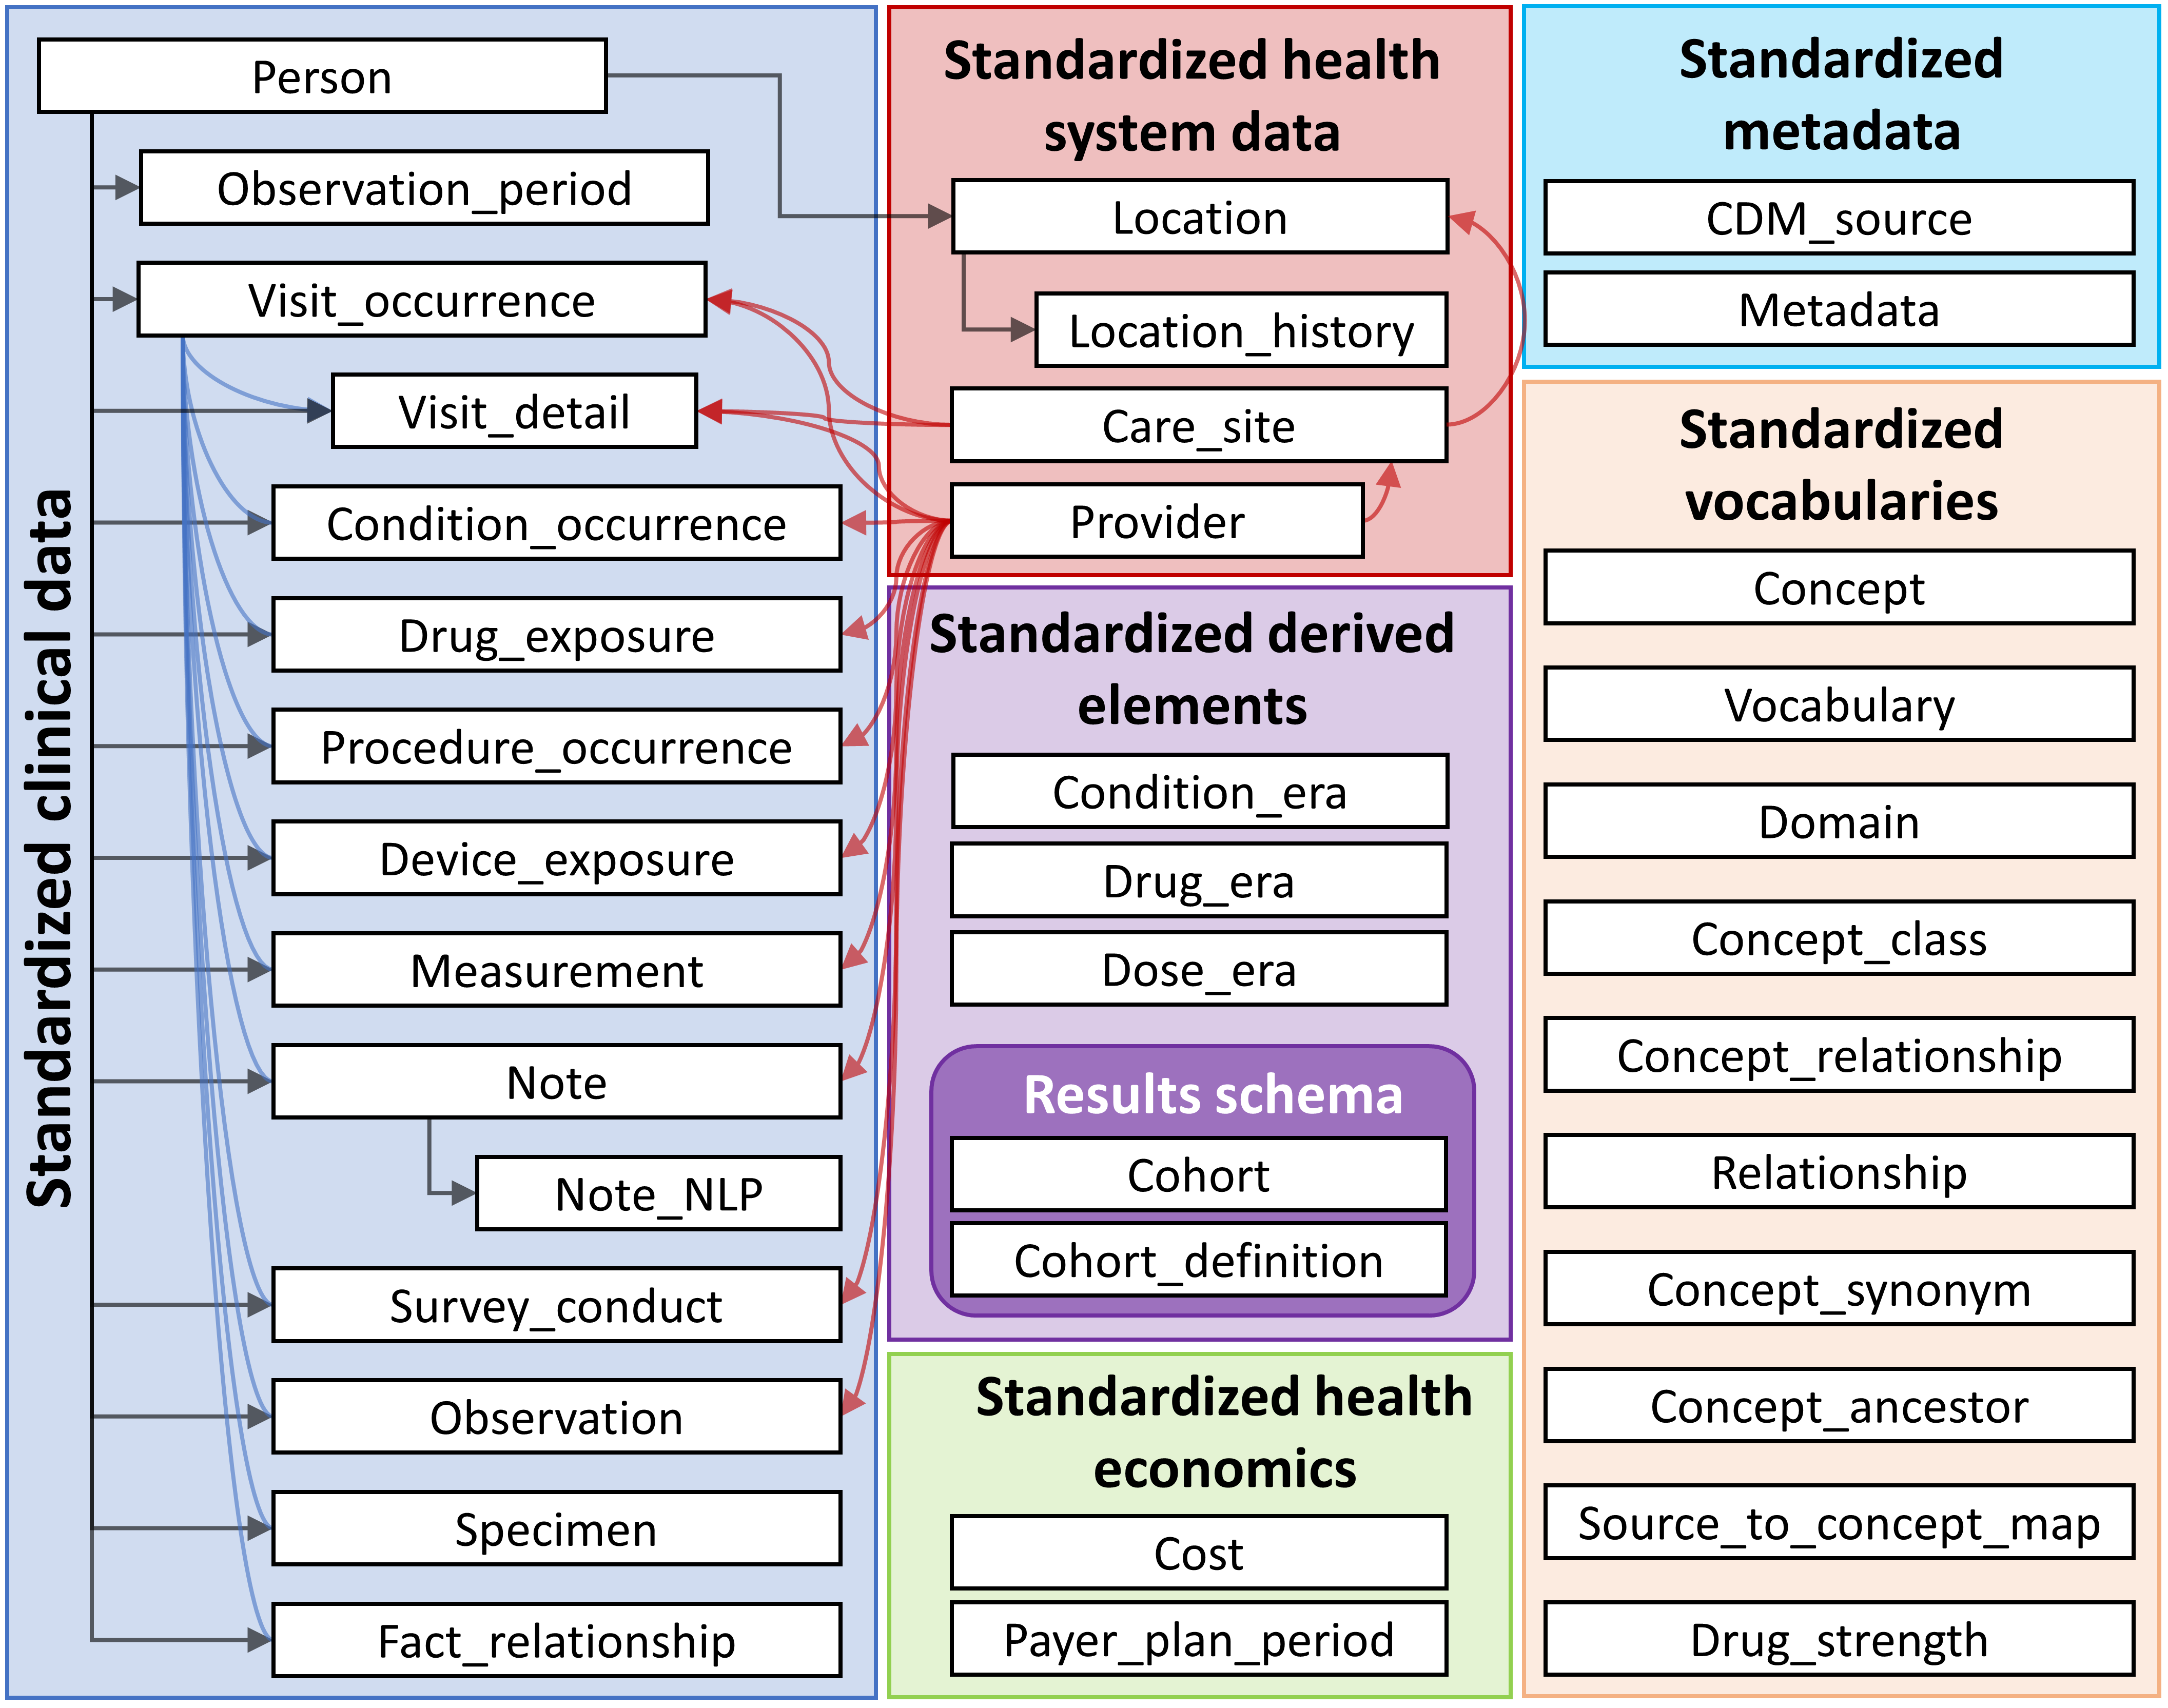
\includegraphics[width=1\linewidth]{images/CommonDataModel/cdmDiagram} \caption{CDM 6.0 버전의 모든 테이블에 대한 개요. 테이블 간의 모든 관계가 표시된 것은 아님.}\label{fig:cdmDiagram}
\end{figure}

\section{설계 원리}\label{-}

CDM은 다음과 같은 목적의 전형적인 관찰 연구에 최적화되어
있다.\index{Common Data Model!design principles}

\begin{itemize}
\tightlist
\item
  특정한 의료 행위의 개입 (약물 노출, 시술(procedure), 의료 정책 변경
  등)이 있거나 의료 관련 결과 (질환, 시술, 기타 약물 노출에 대한)를
  포함하는 환자 집단 확인.
\item
  인구 통계학적 정보, 질병의 자연사, 의료 서비스 전달, 활용 및 비용,
  병적 상태, 치료 및 치료 과정 등과 같은 다양한 매개 변수에 대한 환자
  집단의 특성 확인.
\item
  개별 환자에서 결과의 발생 예측 - \ref{PatientLevelPrediction}장 참고,
\item
  앞서 설명한 의료 행위의 개입이 인구에 미치는 영향 추정 -
  \ref{PopulationLevelEstimation}장 참고,
\end{itemize}

이러한 목표를 달성하기 위해서 CDM의 개발은 다음과 같은 설계 요소를
따른다:

\begin{itemize}
\tightlist
\item
  \textbf{목적에 대한 적합성}: CDM은 의료 서비스 제공이나 보험청구
  업무를 해결하기 위한 목적 보다는 분석에 최적화된 방식으로 구성된
  데이터를 제공하는 것을 목표로 한다.
  \index{Common Data Model!suitability for purpose}
\item
  \textbf{데이터 보호}: 이름, 생년월일 등 환자의 신원 및 안전을 위협할
  수 있는 모든 데이터는 제한되어 있다. 영아에 대한 연구를 위한 정확한
  생년 월일과 같은 보다 자세한 정보가 명시적으로 필요한 경우에는 예외가
  가능하다.\index{Common Data Model!data protection}
\item
  \textbf{도메인 설계}: 도메인은 개인 중심 관계형 데이터
  모델(person-centric relational data model)로 모델링 되며 각 기록마다
  개인의 신원과 날짜 정보가 최소한으로 수집된다. 여기서 관계형 데이터
  모델은 데이터가 기본 키와 외래 키로 연결된 테이블들로 표현되는
  모델이다.
\item
  \textbf{도메인의 이론적 근거}: 개체-관계 모델(entity-relationship
  model)에서 도메인은 분석 이용 사례가 있는지 (예를 들면,
  질환(conditions)) 그리고 달리 적용 가능한 방안이 없는 특정한
  속성(attributes)이 있는지에 따라서 별도로 정의된다. 다른 모든 데이터는
  개체-속성-값 구조(entity-attribute-value structure)를 가진 Observation
  테이블에 관찰 데이터로 저장할 수 있다.
  \index{Common Data Model!domains}
\item
  \textbf{표준화된 어휘}: 기록을 표준화하기 위해, CDM은 필수적이고
  적절한 표준 건강 관리 Concept을 포함하는 표준 어휘에 의존한다.
\item
  \textbf{기존 어휘 재사용}: 이러한 개념은 국립 의학 도서관, 재향 군인
  담당 부서, 질병 통제 및 예방 센터 등과 같은 국가 및 산업 표준화 또는
  용어 정의 주도 기관이나 협회에서 만든 어휘를 재사용하기도 한다.
\item
  \textbf{원본 코드 유지 관리}: 모든 코드가 표준화된 어휘에 매핑되어
  있더라도 정보가 소실되지 않도록 원본 코드도 저장한다.
  \index{Common Data Model!Source Codes}
  \index{Common Data Model!data loss prevention}
\item
  \textbf{기술 중립성}: CDM은 특정 기술만을 채택하지 않는다. Oracle, SQL
  Server 등과 같은 관계형 데이터베이스 또는 SAS 분석 데이터 세트로도
  구현될 수 있다. \index{Common Data Model!technology neutrality}
\item
  \textbf{확장성}: CDM은 데이터 처리 및 컴퓨터를 이용한 분석에
  최적화되어 있기 때문에 수 십 억 건에 달하는 임상 관찰을 비롯하여 수 억
  명이 포함된 데이터베이스 등 다양한 크기의 원천 데이터를 수용할 수
  있다. \index{Common Data Model!scalability}
\item
  \textbf{이전 버전과의 호환성}: 이전 CDM로부터의 모든 변경 사항은
  github 저장소
  \href{https://github.com/OHDSI/CommonDataModel}{(https://github.com/OHDSI/CommonDataModel)}에
  명확하게 서술되어 있다. CDM의 이전 버전은 현재 버전을 이용해 쉽게 만들
  수 있으며, 이전에 있었던 정보는 손실되지 않는다.
  \index{Common Data Model!backwards compatibility}
\end{itemize}

\section{데이터 모델 규칙}\label{--}

CDM에 채택된 많은 묵시적 혹은 명시적인 규칙이 있다. 따라서, CDM에 관련된
메소드 개발자들은 이러한 규칙을 잘 이해하고 있어야 한다.
\index{Common Data Model!conventions}

\subsection{모델의 일반적인 규칙}\label{model-Conv}

CDM은 ``개인 중심''의 모델로서, 모든 임상적인 사건에 대한 테이블이
PERSON 테이블을 중심으로 연결되어 있다. 시작 날짜 및 기타 날짜 정보들과
더불어 이는 모든 의료 관련 사건에 대해 각 사람별로 종적 관찰이
가능하도록 한다. 이 규칙에 예외적으로, 표준화된 의료체계 데이터
테이블(standardized health system data tables)은 다양한 도메인의 사건에
직접 연결되어 있다.

\subsection{스키마의 일반적인 규칙}\label{--}

스키마 또는 데이터베이스 사용자는 읽기 전용 테이블과 읽기/쓰기 테이블을
분리할 수 있다. 임상 사건 및 어휘 테이블은 ``CDM'' 스키마에 저장되어
있으며 최종 사용자 또는 분석 도구에서는 읽기 전용으로 이용된다. 웹 기반
도구 및 최종 사용자가 조작할 필요가 있는 테이블은 ``Outcome'' 스키마에
저장된다. ``Outcome'' 스키마의 두 테이블은 COHORT와
COHORT\_DEFINITON이다. 이 테이블들은 \ref{Cohorts}장에 자세히 설명되어
있는 것처럼 사용자가 정의할 수 있는 관심 그룹을 설명하기 위한 것이다.
이는 분석 중에 테이블이 작성될 수 있음을, 즉 새로 생성한 코호트가 COHORT
테이블에 저장될 수 있다는 것을 의미한다. 모든 사용자를 위한 읽기-쓰기
스키마는 단 하나뿐이므로, 여러 사용자 접근이 어떻게 구성되고
제어되는지는 CDM의 구현에 달려 있다.

\subsection{데이터 테이블의 일반적인 규칙}\label{---}

CDM은 플랫폼에 비의존적이다. 데이터 유형은 일반적으로 ANSI SQL 데이터
유형(VARCHAR, INTEGER, FLOAT, DATE, DATETIME, CLOB)을 사용하여 정의된다.
VARCHAR에서만 정밀도가 제공된다. 이는 필요한 최소 문자열 길이를
반영하지만 구체적인 CDM 인스턴스 내에서 확장할 수 있다. CDM은 날짜 및
날짜시간 형식을 규정하지 않는다. CDM에 대한 표준 쿼리는 로컬 인스턴스 및
날짜/시간 구성에 따라 달라질 수 있다.

\emph{참고}: 데이터 모델 자체는 플랫폼에 독립적이지만, 데이터 모델과
함께 작동하도록 구축된 여러 도구는 특정 사양이 요구된다. 이에 대한
자세한 내용은 \ref{OhdsiAnalyticsTools}장 참조.

\subsection{도메인의 일반적인 규칙}\label{domains}

서로 다른 성격의 사건들은 도메인 별로 정리되어 있다. 이러한 사건들은
도메인별로 테이블과 필드에 저장되고, 표준화된 어휘에 정의되어 있는 대로
도메인별 표준 Concept으로 표현된다 (\ref{conceptDomains}절 참조). 각
표준 Concept에 고유한 도메인이 할당되는데, 이는 어떤 테이블에 기록되어야
하는지를 정의한다. 정확한 도메인 할당은 커뮤니티내에서 항상 논의의
대상이 되지만, 엄격한 도메인-테이블-필드간 대응 규칙은 어떠한 코드나
Concept에 대해서도 항상 정확성을 보장한다. 예를 들어, 증상 및 진단
Concept은 Condition 도메인에 속하며 Condition\_OCCURRENCE 테이블의
CONDITION\_CONCEP\_ID로 기록된다. 소위 말하는 시술시 사용되는 약품은
일반적으로 원천 데이터에서는 Procedure 테이블에 Procedure 코드로
기록되지만, CDM에서는 이러한 정보는 매핑된 표준 Concept이 약물 도메인에
할당 되어있기 때문에 DRUG\_EXPOSURE 테이블에 저장한다. 표
\ref{tab:domains}과 같이 총 30개의 도메인이 있다.

\begin{longtable}[]{@{}llll@{}}
\caption{\label{tab:domains} 각 도메인에 속하는 표준 Concept의
수.}\tabularnewline
\toprule
Concept Count & Domain ID & Concept Count & Domain ID\tabularnewline
\midrule
\endfirsthead
\toprule
Concept Count & Domain ID & Concept Count & Domain ID\tabularnewline
\midrule
\endhead
1731378 & Drug & 183 & Route\tabularnewline
477597 & Device & 180 & Currency\tabularnewline
257000 & Procedure & 158 & Payer\tabularnewline
163807 & Condition & 123 & Visit\tabularnewline
145898 & Observation & 51 & Cost\tabularnewline
89645 & Measurement & 50 & Race\tabularnewline
33759 & Spec Anatomic Site & 13 & Plan Stop Reason\tabularnewline
17302 & Meas Value & 11 & Plan\tabularnewline
1799 & Specimen & 6 & Episode\tabularnewline
1215 & Provider Specialty & 6 & Sponsor\tabularnewline
1046 & Unit & 5 & Meas Value Operator\tabularnewline
944 & Metadata & 3 & Spec Disease Status\tabularnewline
538 & Revenue Code & 2 & Gender\tabularnewline
336 & Type Concept & 2 & Ethnicity\tabularnewline
194 & Relationship & 1 & Observation Type\tabularnewline
\bottomrule
\end{longtable}

\subsection{Concept을 통한 내용 표현}\label{concept---}

CDM 테이블에서는 각 정보의 내용이 완전히 정규화되어 Concept으로
저장된다. Concept은 CONCEPT 테이블의 외래 키 역할을 하는 각각의
CONCEPT\_ID 값이 할당되어 사건 테이블에 저장된다. CDM의 모든 인스턴스는
(Concept에 대한 참고 자료로써 공통 데이터 모델과 함께 상호운용의 핵심
메커니즘이자 OHDSI 연구 네트워크의 기반인) 동일한 CONCEPT 테이블을
사용한다. 표준 Concept이 없거나 식별되지 않는 경우에는 CONCEPT\_ID가
존재하지 않는 Concept이거나 알 수 없음 또는 매핑이 불가능함을 의미하는
0으로 설정된다 (즉, CONCEPT\_ID = 0).

CONCEPT 테이블의 정보는 각각의 Concept에 대한 상세 정보 (이름, 도메인,
클래스 등) 를 포함하고 있다. Concepts, Concept Relationships, Concept
Ancestors 및 다른 Concept과 관련 있는 정보들은 표준화된 용어에 포함되어
있다 (\ref{StandardizedVocabularies}장 참조).

\subsection{필드 명명 규칙}\label{--}

모든 테이블의 변수명은 하나의 규칙을 따른다:

\begin{longtable}[]{@{}ll@{}}
\caption{\label{tab:fieldConventions} 필드 명 규칙.}\tabularnewline
\toprule
\begin{minipage}[b]{0.34\columnwidth}\raggedright\strut
Notation\strut
\end{minipage} & \begin{minipage}[b]{0.60\columnwidth}\raggedright\strut
Description\strut
\end{minipage}\tabularnewline
\midrule
\endfirsthead
\toprule
\begin{minipage}[b]{0.34\columnwidth}\raggedright\strut
Notation\strut
\end{minipage} & \begin{minipage}[b]{0.60\columnwidth}\raggedright\strut
Description\strut
\end{minipage}\tabularnewline
\midrule
\endhead
\begin{minipage}[t]{0.34\columnwidth}\raggedright\strut
{[}Event{]}\_ID\strut
\end{minipage} & \begin{minipage}[t]{0.60\columnwidth}\raggedright\strut
각 행의 고유 식별자로, 사건 테이블간 관계를 설정하는 외래 키 역할을
한다. 예를 들어 PERSON\_ID는 각 개인을 고유하게 식별한다.
VISIT\_OCCURRENCE\_ID는 방문을 고유하게 식별한다.\strut
\end{minipage}\tabularnewline
\begin{minipage}[t]{0.34\columnwidth}\raggedright\strut
{[}Event{]}\_CONCEPT\_ID\strut
\end{minipage} & \begin{minipage}[t]{0.60\columnwidth}\raggedright\strut
CONCEPT 참고 테이블의 표준 Concept에 대한 외래 키. 이는 모든 분석에
기반이 되는 사건의 주요 표현이다. 예를 들어 CONDITION\_CONCEPT\_ID =
\href{http://athena.ohdsi.org/search-terms/terms/31967}{31967}에는
SNOMED Concept인 ``오심 Nausea''에 대한 참조 값을 포함하고 있다.\strut
\end{minipage}\tabularnewline
\begin{minipage}[t]{0.34\columnwidth}\raggedright\strut
{[}Event{]}\_SOURCE \_CONCEPT\_ID\strut
\end{minipage} & \begin{minipage}[t]{0.60\columnwidth}\raggedright\strut
CONCEPT 참고 테이블의 행에 대한 외래 키. 이 Concept은 원본 값(아래)과
동등하며, 이때 {[}EVENT\_CONCEPT\_ID{]}와 동일한 표준 개념이거나 또 다른
비-표준 concept일 수 있다. 예를 들어, Condition\_SOURCE\_CONCEPT\_ID =
\href{http://athena.ohdsi.org/search-terms/terms/45431665}{45431665}는
READ 용어집의 ``Nausea'' 개념을 나타내며, 유사한
CONDITION\_CONCEPT\_ID는 표준 SNOMED-CT concept으로
\href{http://athena.ohdsi.org/search-terms/terms/31967}{31967}이다. 표준
Concept만이 사건의 의미를 모호하지 않게 표현하므로 표준 분석에 응용 시
상호 운용성이 없는 원본 개념(SOURCE \_CONCEPT)을 사용하는 것은
바람직하지 않다.\strut
\end{minipage}\tabularnewline
\begin{minipage}[t]{0.34\columnwidth}\raggedright\strut
{[}Event{]}\_TYPE\_CONCEPT\_ID\strut
\end{minipage} & \begin{minipage}[t]{0.60\columnwidth}\raggedright\strut
원본 정보의 출처를 나타내는 CONCEPT 참고 테이블(CONCEPT reference
table)에 대한 외래 키. 이는 사건의 유형이나 concept의 유형을 나타내는
것이 아니라 이 기록를 생성한 메커니즘에 대한 정보를 수집하는 것을
의미한다. 예를 들면, DRUG\_TYPE\_CONCEPT\_ID는 이 기록이 약국에서의 처방
(``Pharmacy dispensing'') 으로 부터 발생하였는지 혹은 전자 처방 신청서
(``Prescription written'') 로부터 발생하였는지를 구분한다.\strut
\end{minipage}\tabularnewline
\begin{minipage}[t]{0.34\columnwidth}\raggedright\strut
{[}Event{]}\_SOURCE\_VALUE\strut
\end{minipage} & \begin{minipage}[t]{0.60\columnwidth}\raggedright\strut
이 사건이 원천 데이터에 표현되어 있는 방식 그대로 쓰여진 코드 혹은
자유서술 문자열이다. 이 원본 값들은 데이터 원본간에 통일되어 있지
않으므로 표준 분석 방식에 사용하는 것은 좋지 않다. 예를 들면,
CONDITION\_SOURCE\_VALUE는 ICD-9 코드 787.02에 점을 제외하고
``78702''라는 기록를 포함할 수 있다.\strut
\end{minipage}\tabularnewline
\bottomrule
\end{longtable}

\subsection{concept과 원본 값과의 차이}\label{concepts-Sources}

많은 테이블이 원본 값, 원본 concept, 표준 concept으로 다양한 위치에
동일한 정보를 포함하고 있다.

\begin{itemize}
\tightlist
\item
  \textbf{Source Values} 은 원천 데이터에서의 사건 기록의 본래 표현이다.
  이는 ICD9CM, NDC 또는 Read와 같은 널리 사용되는 공공 도메인의 코딩
  시스템이나 CPT4, GPI 또는 MedDRA와 같이 독점적인 코딩 시스템, 혹은
  남성은 M 여성은 F와 같이 원천 데이터에서만 사용되는 제한된 어휘의
  코드일 수 있다. 또한 표준화 및 제어되지 않은 짧은 자유 텍스트 문구 일
  수도 있다. 원본 값은 데이터 테이블의 {[}Event{]} \_SOURCE\_VALUE
  필드에 저장된다. concept은 임상적 요소의 의미를 일반화하는 CDM
  특이적인 개체이다. 대부분의 concept은 이미 의료계에 존재하는
  공개되었거나 독점적인 코딩 체계를 기반으로 하고 있지만, 일부는 새롭게
  생성되었다 (CONCEPT\_CODE는 ``OMOP''으로부터 시작됨). concept은 모든
  도메인에 걸쳐 고유한 ID를 가지고 있다.
\item
  \textbf{Concepts} 은 임상적 요소의 의미를 일반화하는 CDM 특이적인
  개체이다. 대부분의 concept은 이미 의료계에 존재하는 공개되었거나
  독점적인 코딩 체계를 기반으로 하고 있지만, 일부는 새롭게 생성되었다
  (CONCEPT\_CODE는 ``OMOP''으로부터 시작됨). concept은 모든 도메인에
  걸쳐 고유한 ID를 가지고 있다.
\item
  \textbf{Source Concepts} 은 원 자료에서 사용된 코드를 나타내는
  concept이다. 원본 concept은 OMOP기반의 concept이 아니라 기존에
  존재하는 공개되었거나 독점적인 코딩 체계만을 위해 사용한다. 원본
  concept은 데이터 테이블의 {[}Event{]} \_SOURCE\_CONCEPT\_ID 필드에
  저장된다.
\item
  \textbf{Standard Concepts} 은 모든 데이터 베이스에서 고유하게 임상적인
  개체의 의미를 정의하는 데에 사용되고 원본에서 사용한 코딩 체계와는
  독립적인 concept이다. 표준 concept은 일반적으로 이미 공개되어 있거나
  독점적인 용어 원본에서 가져온다. 표준 concept과 동일한 의미를 가진 비
  표준 concept은 표준 용어의 표준 concept에 매핑되어 있다. 표준
  concept은 데이터 테이블의 {[}Event{]} \_CONCEPT\_ID 필드에서 참조된다.
\end{itemize}

원본 값은 편의 및 품질 보증(Quality Assurance, QA) 목적으로만 제공된다.
여기에는 특정 데이터 원본의 맥락에서만 의미 있는 정보가 포함될 수 있다.
원본 값이나 원본 concept을 사용하는 것은 선택사항이지만, 원본 데이터가
코딩 시스템을 사용하는 경우 \textbf{강력하게 권장}된다. 하지만 표준
concept의 경우 \textbf{필수 사항}이다. 이 표준 concept을 필수적으로
사용하면 모든 CDM 인스턴스가 동일한 언어를 사용할 수 있다. 예를 들면
``Pulmonary Tuberculosis'' (TB, 그림 \ref{fig:pulmTubICD9}참조)의
condition은 TB에 대한 ICD9CM 코드가 011임을 나타낸다.

\begin{figure}

{\centering 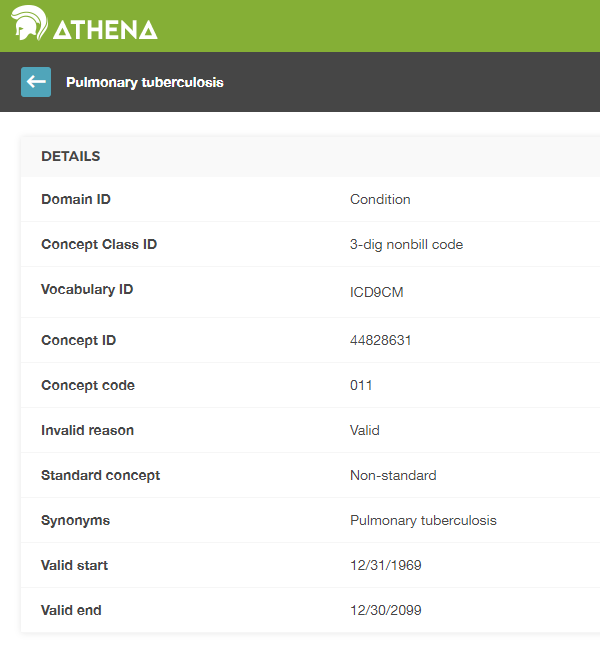
\includegraphics[width=0.75\linewidth]{images/CommonDataModel/pulmTubICD9} 

}

\caption{Pulmonary Tuberculosis의 ICD9CM 코드}\label{fig:pulmTubICD9}
\end{figure}

문맥이 없으면, 코드 011은 UB04 언어의 ``Hospital Inpatient (Including
Medicare Part A)''로 해석되거나, DRG 용어의 ``Nervous System Neoplasms
without Complications, Comorbidities''로 해석될 수 있다. 이것이 원본와
표준 모두의 concept ID가 중요한 이유이다. 011인 ICD9CM 코드를 나타내는
CONCEPT\_ID 값은
\href{http://athena.ohdsi.org/search-terms/terms/44828631}{44828631}이다.
이는 ICD9CM을 UBO4 및 DRG와 구별한다. ICD9CM의 TB 원본 concept은 그림
\ref{fig:pulmTubMap}과 같이``OMOP (Non-standard to Standard Map)''관계를
통해 SNOMED 어휘에서 표준 concept
\href{http://athena.ohdsi.org/search-terms/terms/253954}{253954}로
매핑된다. 표준 SNOMED 개념을 참조하는 모든 연구가 지원되는 모든 원본
코드를 포함할 수 있도록 Read, ICD10, CIEL 및 MeSH 코드에도 동일한 매핑
관계가 존재한다.

\begin{figure}

{\centering 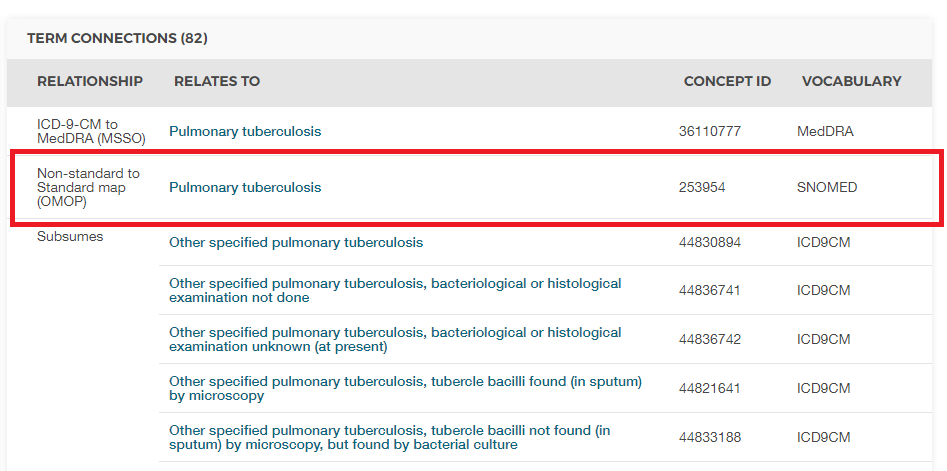
\includegraphics[width=1\linewidth]{images/CommonDataModel/pulmTubMap} 

}

\caption{Pulmonary Tuberculosis의 SNOMED 코드}\label{fig:pulmTubMap}
\end{figure}

표준 concept과 원본 concept의 관계를 보여주는 예가 표
\ref{tab:conditionOccurrence}에 나와있다.

\section{표준화된 CDM 테이블}\label{-cdm-}

\index{Common Data Model!standardized tables}

CDM에는 16개의 임상 사건 테이블, 10개의 어휘 테이블, 2개의 메타데이터
테이블, 4개의 보건 시스템 데이터 테이블, 2개의 보건 경제학 데이터
테이블, 3개의 표준화된 파생 요소 및 2개의 결과 스키마 테이블이 포함되어
있다. 이 테이블들은 CDM Wiki에 전체 명시되어 있다.\footnote{\url{https://github.com/OHDSI/CommonDataModel/wiki}}

이러한 테이블들이 실제로 어떻게 사용되는지를 설명하기 위해, 한 사람의
데이터를 이 장의 나머지 부분에서 걸쳐 공통으로 사용할 것이다.

\subsection{실행 예제: 자궁내막증}\label{--}

자궁내막증은 보통 여성의 자궁 내 표피에 있는 자궁내막세포가 신체 다른
곳에서 생겨나는 고통스러운 질환이다. 심한 경우는 불임, 장, 방광 문제를
일으킬 수 있다. 해당 섹션에서는 한 환자의 이 질병에 대한 경험과 이
질병이 공통 데이터 모델로 어떻게 표현되는지를 상세하게 설명하고자 한다.

\begin{center}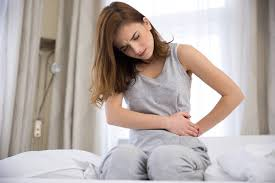
\includegraphics[width=0.5\linewidth]{images/CommonDataModel/Lauren} \end{center}

\begin{quote}
나는 이 고통스러운 여정의 모든 과정마다 내가 얼마만큼의 고통을 받고
있는지를 모두에게 납득시켜야 했다.
\end{quote}

Lauren은 수년 동안 자궁 내막증 증상을 겪어 왔다. 그러나 진단을 받기 전에
난소에서 낭종이 파열되었다. Lauren에 대한 자세한 내용은
\url{https://www.endometriosis-uk.org/laurens-story}에서 확인할 수 있다.

\subsection{PERSON 테이블}\label{person}

\subsubsection*{Lauren에 대해서 우리가 알고 있는
것은?}\label{lauren-----}
\addcontentsline{toc}{subsubsection}{Lauren에 대해서 우리가 알고 있는
것은?}

\begin{itemize}
\tightlist
\item
  그녀는 36세 여성이다
\item
  그녀의 생년월일은 1982년 3월 12일이다
\item
  그녀는 백인이다
\item
  그녀는 영국인이다
\end{itemize}

이를 염두에 두면 PERSON 테이블을 다음과 같이 나타낼 수 있다:

\begin{longtable}[]{@{}lll@{}}
\caption{\label{tab:person} PERSON 테이블.}\tabularnewline
\toprule
\begin{minipage}[b]{0.28\columnwidth}\raggedright\strut
Column name\strut
\end{minipage} & \begin{minipage}[b]{0.16\columnwidth}\raggedright\strut
Value\strut
\end{minipage} & \begin{minipage}[b]{0.48\columnwidth}\raggedright\strut
Explanation\strut
\end{minipage}\tabularnewline
\midrule
\endfirsthead
\toprule
\begin{minipage}[b]{0.28\columnwidth}\raggedright\strut
Column name\strut
\end{minipage} & \begin{minipage}[b]{0.16\columnwidth}\raggedright\strut
Value\strut
\end{minipage} & \begin{minipage}[b]{0.48\columnwidth}\raggedright\strut
Explanation\strut
\end{minipage}\tabularnewline
\midrule
\endhead
\begin{minipage}[t]{0.28\columnwidth}\raggedright\strut
PERSON\_ID\strut
\end{minipage} & \begin{minipage}[t]{0.16\columnwidth}\raggedright\strut
1\strut
\end{minipage} & \begin{minipage}[t]{0.48\columnwidth}\raggedright\strut
PERSON\_ID는 원본에서 직접적으로 생성되거나 빌드 과정의 일부분으로
생성된 정수여야 한다.\strut
\end{minipage}\tabularnewline
\begin{minipage}[t]{0.28\columnwidth}\raggedright\strut
GENDER\_CONCEPT\_ID\strut
\end{minipage} & \begin{minipage}[t]{0.16\columnwidth}\raggedright\strut
8532\strut
\end{minipage} & \begin{minipage}[t]{0.48\columnwidth}\raggedright\strut
여성을 의미하는 concept ID는
\href{http://athena.ohdsi.org/search-terms/terms/8532}{8532}이다.\strut
\end{minipage}\tabularnewline
\begin{minipage}[t]{0.28\columnwidth}\raggedright\strut
YEAR\_OF\_BIRTH\strut
\end{minipage} & \begin{minipage}[t]{0.16\columnwidth}\raggedright\strut
1982\strut
\end{minipage} & \begin{minipage}[t]{0.48\columnwidth}\raggedright\strut
\strut
\end{minipage}\tabularnewline
\begin{minipage}[t]{0.28\columnwidth}\raggedright\strut
MONTH\_OF\_BIRTH\strut
\end{minipage} & \begin{minipage}[t]{0.16\columnwidth}\raggedright\strut
3\strut
\end{minipage} & \begin{minipage}[t]{0.48\columnwidth}\raggedright\strut
\strut
\end{minipage}\tabularnewline
\begin{minipage}[t]{0.28\columnwidth}\raggedright\strut
DAY\_OF\_BIRTH\strut
\end{minipage} & \begin{minipage}[t]{0.16\columnwidth}\raggedright\strut
12\strut
\end{minipage} & \begin{minipage}[t]{0.48\columnwidth}\raggedright\strut
\strut
\end{minipage}\tabularnewline
\begin{minipage}[t]{0.28\columnwidth}\raggedright\strut
BIRTH\_DATETIME\strut
\end{minipage} & \begin{minipage}[t]{0.16\columnwidth}\raggedright\strut
1982-03-12 00:00:00\strut
\end{minipage} & \begin{minipage}[t]{0.48\columnwidth}\raggedright\strut
시간을 정확히 알 수 없는 경우 자정으로 한다.\strut
\end{minipage}\tabularnewline
\begin{minipage}[t]{0.28\columnwidth}\raggedright\strut
DEATH\_DATETIME\strut
\end{minipage} & \begin{minipage}[t]{0.16\columnwidth}\raggedright\strut
\strut
\end{minipage} & \begin{minipage}[t]{0.48\columnwidth}\raggedright\strut
\strut
\end{minipage}\tabularnewline
\begin{minipage}[t]{0.28\columnwidth}\raggedright\strut
RACE\_CONCEPT\_ID\strut
\end{minipage} & \begin{minipage}[t]{0.16\columnwidth}\raggedright\strut
8527\strut
\end{minipage} & \begin{minipage}[t]{0.48\columnwidth}\raggedright\strut
백인을 의미하는 concept ID는
\href{http://athena.ohdsi.org/search-terms/terms/8527}{8527}이다.
영국인이라는 민족성은
\href{http://athena.ohdsi.org/search-terms/terms/4093769}{4093769}이다.
둘 다 해당할 경우 전자를 활용한다. 민족성은 ETHNICITY\_CONCEPT\_ID가
아닌 인종의 일부로써 여기에 저장된다.\strut
\end{minipage}\tabularnewline
\begin{minipage}[t]{0.28\columnwidth}\raggedright\strut
ETHNICITY\_CONCEPT\_ ID\strut
\end{minipage} & \begin{minipage}[t]{0.16\columnwidth}\raggedright\strut
38003564\strut
\end{minipage} & \begin{minipage}[t]{0.48\columnwidth}\raggedright\strut
이는 히스패닉을 다른 사람들과 구분하기 위해 사용되는 전형적인 미국식
표기법이다. 이 경우 영국인인 민족성은 RACE\_CONCEPT\_ID에 저장된다. 미국
이외의 지역에서는 사용되지 않는다.
\href{http://athena.ohdsi.org/search-terms/terms/38003564}{38003564}는
``히스패닉이 아님''을 나타낸다.\strut
\end{minipage}\tabularnewline
\begin{minipage}[t]{0.28\columnwidth}\raggedright\strut
LOCATION\_ID\strut
\end{minipage} & \begin{minipage}[t]{0.16\columnwidth}\raggedright\strut
\strut
\end{minipage} & \begin{minipage}[t]{0.48\columnwidth}\raggedright\strut
주소는 알려져 있지 않다.\strut
\end{minipage}\tabularnewline
\begin{minipage}[t]{0.28\columnwidth}\raggedright\strut
PROVIDER\_ID\strut
\end{minipage} & \begin{minipage}[t]{0.16\columnwidth}\raggedright\strut
\strut
\end{minipage} & \begin{minipage}[t]{0.48\columnwidth}\raggedright\strut
일차 진료 제공자는 알려져 있지 않다.\strut
\end{minipage}\tabularnewline
\begin{minipage}[t]{0.28\columnwidth}\raggedright\strut
CARE\_SITE\strut
\end{minipage} & \begin{minipage}[t]{0.16\columnwidth}\raggedright\strut
\strut
\end{minipage} & \begin{minipage}[t]{0.48\columnwidth}\raggedright\strut
일차 진료 장소는 알려져 있지 않다.\strut
\end{minipage}\tabularnewline
\begin{minipage}[t]{0.28\columnwidth}\raggedright\strut
PERSON\_SOURCE\_ VALUE\strut
\end{minipage} & \begin{minipage}[t]{0.16\columnwidth}\raggedright\strut
1\strut
\end{minipage} & \begin{minipage}[t]{0.48\columnwidth}\raggedright\strut
대부분 PERSON\_ID 와 동일 하지만 일반적으로 이는 원본 데이터에서의
그녀의 식별자가 될 것이다.\strut
\end{minipage}\tabularnewline
\begin{minipage}[t]{0.28\columnwidth}\raggedright\strut
GENDER\_SOURCE\_ VALUE\strut
\end{minipage} & \begin{minipage}[t]{0.16\columnwidth}\raggedright\strut
F\strut
\end{minipage} & \begin{minipage}[t]{0.48\columnwidth}\raggedright\strut
원본에 나타난 성별에 대한 값이 여기에 저장되어 있다.\strut
\end{minipage}\tabularnewline
\begin{minipage}[t]{0.28\columnwidth}\raggedright\strut
GENDER\_SOURCE\_ CONCEPT\_ID\strut
\end{minipage} & \begin{minipage}[t]{0.16\columnwidth}\raggedright\strut
0\strut
\end{minipage} & \begin{minipage}[t]{0.48\columnwidth}\raggedright\strut
원본의 성별에 대한 값이 OHDSI에서 지원하는 코딩 체계를 사용한 경우 해당
concept이 여기에 해당한다. 예를 들어, 그녀의 성별이 원본에서
``sex-F''이고 PCORNet 어휘 concept에 있다고 언급되어 있다면
\href{http://athena.ohdsi.org/search-terms/terms/44814665}{44814665}이
이 필드에 입력될 것이다.\strut
\end{minipage}\tabularnewline
\begin{minipage}[t]{0.28\columnwidth}\raggedright\strut
RACE\_SOURCE\_ VALUE\strut
\end{minipage} & \begin{minipage}[t]{0.16\columnwidth}\raggedright\strut
white\strut
\end{minipage} & \begin{minipage}[t]{0.48\columnwidth}\raggedright\strut
인종 값이 원본에 있는대로 여기에 저장된다.\strut
\end{minipage}\tabularnewline
\begin{minipage}[t]{0.28\columnwidth}\raggedright\strut
RACE\_SOURCE\_ CONCEPT\_ID\strut
\end{minipage} & \begin{minipage}[t]{0.16\columnwidth}\raggedright\strut
0\strut
\end{minipage} & \begin{minipage}[t]{0.48\columnwidth}\raggedright\strut
GENDER\_CONCEPT\_ID와 같은 원리 적용.\strut
\end{minipage}\tabularnewline
\begin{minipage}[t]{0.28\columnwidth}\raggedright\strut
ETHNICITY\_SOURCE\_ VALUE\strut
\end{minipage} & \begin{minipage}[t]{0.16\columnwidth}\raggedright\strut
english\strut
\end{minipage} & \begin{minipage}[t]{0.48\columnwidth}\raggedright\strut
민족성 값이 원본에 나와 있는대로 여기에 저장된다.\strut
\end{minipage}\tabularnewline
\begin{minipage}[t]{0.28\columnwidth}\raggedright\strut
ETHNICITY\_SOURCE\_ CONCEPT\_ID\strut
\end{minipage} & \begin{minipage}[t]{0.16\columnwidth}\raggedright\strut
0\strut
\end{minipage} & \begin{minipage}[t]{0.48\columnwidth}\raggedright\strut
GENDER\_SOURCE\_CONCEPT\_ID와 같은 원리 적용.\strut
\end{minipage}\tabularnewline
\bottomrule
\end{longtable}

\subsection{OBSERVATION\_PERIOD 테이블}\label{observationPeriod}

OBSERVATION\_PERIOD 테이블은 최소한 환자의 인구통계, 질환, 시술 및
약물이 원본 시스템에 기록되는 시간을 민감성과 특수성을 고려하여 합리적인
예상을 통해 정의하도록 설계되었다. 보험 데이터의 경우 일반적으로 환자의
등록 시기이다. 대부분의 의료 시스템이 어떤 의료 기관이나 제공업체를
방문할지 결정해두지 않기 때문에 전자 의무 기록(EHR)에서는 더욱 까다롭다.
차선책으로서 시스템의 첫 번째 기록은 관측 기간의 시작일로 간주되고
마지막 기록은 종료일로 간주된다.

\subsubsection*{Lauren의 Observation Period는 어떻게
정의될까?}\label{lauren-observation-period--}
\addcontentsline{toc}{subsubsection}{Lauren의 Observation Period는
어떻게 정의될까?}

표 \ref{tab:encounters}에 나타난 Lauren의 정보가 전자 의무 기록(EHR)
시스템에 기록되었다고 가정하자. 그녀의 관찰 기간에서 얻어진 방문기록은
다음과 같다:

\begin{longtable}[]{@{}llll@{}}
\caption{\label{tab:encounters} Lauren의 의료 기관 방문.}\tabularnewline
\toprule
Encounter ID & Start date & Stop date & Type\tabularnewline
\midrule
\endfirsthead
\toprule
Encounter ID & Start date & Stop date & Type\tabularnewline
\midrule
\endhead
70 & 2010-01-06 & 2010-01-06 & outpatient\tabularnewline
80 & 2011-01-06 & 2011-01-06 & outpatient\tabularnewline
90 & 2012-01-06 & 2012-01-06 & outpatient\tabularnewline
100 & 2013-01-07 & 2013-01-07 & outpatient\tabularnewline
101 & 2013-01-14 & 2013-01-14 & ambulatory\tabularnewline
102 & 2013-01-17 & 2013-01-24 & inpatient\tabularnewline
\bottomrule
\end{longtable}

방문기록을 기반으로 했을 때 그녀의 OBSERVATION\_PERIOD 테이블은 다음과
같을 것이다:

\begin{longtable}[]{@{}lll@{}}
\caption{\label{tab:observationPeriod} OBSERVATION\_PERIOD
테이블.}\tabularnewline
\toprule
\begin{minipage}[b]{0.29\columnwidth}\raggedright\strut
Column name\strut
\end{minipage} & \begin{minipage}[b]{0.14\columnwidth}\raggedright\strut
Value\strut
\end{minipage} & \begin{minipage}[b]{0.48\columnwidth}\raggedright\strut
Explanation\strut
\end{minipage}\tabularnewline
\midrule
\endfirsthead
\toprule
\begin{minipage}[b]{0.29\columnwidth}\raggedright\strut
Column name\strut
\end{minipage} & \begin{minipage}[b]{0.14\columnwidth}\raggedright\strut
Value\strut
\end{minipage} & \begin{minipage}[b]{0.48\columnwidth}\raggedright\strut
Explanation\strut
\end{minipage}\tabularnewline
\midrule
\endhead
\begin{minipage}[t]{0.29\columnwidth}\raggedright\strut
OBSERVATION\_ PERIOD\_ID\strut
\end{minipage} & \begin{minipage}[t]{0.14\columnwidth}\raggedright\strut
1\strut
\end{minipage} & \begin{minipage}[t]{0.48\columnwidth}\raggedright\strut
이는 일반적으로 테이블의 각 기록에 대한 고유 식별자를 생성하는 자동으로
생성되는 값이다.\strut
\end{minipage}\tabularnewline
\begin{minipage}[t]{0.29\columnwidth}\raggedright\strut
PERSON\_ID\strut
\end{minipage} & \begin{minipage}[t]{0.14\columnwidth}\raggedright\strut
1\strut
\end{minipage} & \begin{minipage}[t]{0.48\columnwidth}\raggedright\strut
PERSON 테이블에서 Laura의 기록에 대한 외래 키이며 PERSON을
OBSERVATION\_PERIOD 테이블에 연결한다.\strut
\end{minipage}\tabularnewline
\begin{minipage}[t]{0.29\columnwidth}\raggedright\strut
OBSERVATION\_PERIOD\_ START\_DATE\strut
\end{minipage} & \begin{minipage}[t]{0.14\columnwidth}\raggedright\strut
2010-01-06\strut
\end{minipage} & \begin{minipage}[t]{0.48\columnwidth}\raggedright\strut
이는 기록상 그녀의 가장 처음 방문했을 때 시작 날짜이다.\strut
\end{minipage}\tabularnewline
\begin{minipage}[t]{0.29\columnwidth}\raggedright\strut
OBSERVATION\_PERIOD\_ END\_DATE\strut
\end{minipage} & \begin{minipage}[t]{0.14\columnwidth}\raggedright\strut
2013-01-24\strut
\end{minipage} & \begin{minipage}[t]{0.48\columnwidth}\raggedright\strut
이는 기록상 그녀의 가장 마지막 방문했을 때 마지막 날짜이다.\strut
\end{minipage}\tabularnewline
\begin{minipage}[t]{0.29\columnwidth}\raggedright\strut
PERIOD\_TYPE\_ CONCEPT\_ID\strut
\end{minipage} & \begin{minipage}[t]{0.14\columnwidth}\raggedright\strut
44814725\strut
\end{minipage} & \begin{minipage}[t]{0.48\columnwidth}\raggedright\strut
concept의 클래스가 ``Obs Period Type''인 어휘에서 가장 좋은 선택은
\href{http://athena.ohdsi.org/search-terms/terms/44814724}{44814724}이며,
이는 ``의료 관련 방문 기간(Period covering healthcare encounters)''을
나타낸다.\strut
\end{minipage}\tabularnewline
\bottomrule
\end{longtable}

\subsection{VISIT\_OCCURRENCE}\label{visitOccurrence}

VISIT\_OCCURRENCE에서는 환자의 의료 시스템에 방문한 정보에 대해 저장되어
있다. OHDSI 언어내에서 이를 Visit이라고 하며 주요한 사건로 간주한다.
의료 서비스가 제공될 수 있는 다양한 환경을 나타내는 광범위한 계층 구조를
가진 12 가지 주요 방문 카테고리가 있다. 가장 일반적인 Visit 기록는
입원(inpatient), 외래(outpatient), 응급실(emergency department) 및
비-의료 기관방문(non-medical institution Visits)이다.

\subsubsection*{Lauren의 방문을 Visit으로 어떻게 표현할 수
있을까?}\label{lauren--visit----}
\addcontentsline{toc}{subsubsection}{Lauren의 방문을 Visit으로 어떻게
표현할 수 있을까?}

예를 들어 VISIT\_OCCURRENCE 테이블의 표 \ref{tab:encounters}의 입원 환자
방문을 나타내어 보자.

\begin{longtable}[]{@{}lll@{}}
\caption{\label{tab:visitOccurrence} VISIT\_OCCURRENCE
테이블.}\tabularnewline
\toprule
\begin{minipage}[b]{0.28\columnwidth}\raggedright\strut
Column name\strut
\end{minipage} & \begin{minipage}[b]{0.16\columnwidth}\raggedright\strut
Value\strut
\end{minipage} & \begin{minipage}[b]{0.48\columnwidth}\raggedright\strut
Explanation\strut
\end{minipage}\tabularnewline
\midrule
\endfirsthead
\toprule
\begin{minipage}[b]{0.28\columnwidth}\raggedright\strut
Column name\strut
\end{minipage} & \begin{minipage}[b]{0.16\columnwidth}\raggedright\strut
Value\strut
\end{minipage} & \begin{minipage}[b]{0.48\columnwidth}\raggedright\strut
Explanation\strut
\end{minipage}\tabularnewline
\midrule
\endhead
\begin{minipage}[t]{0.28\columnwidth}\raggedright\strut
VISIT\_OCCURRENCE\_ ID\strut
\end{minipage} & \begin{minipage}[t]{0.16\columnwidth}\raggedright\strut
514\strut
\end{minipage} & \begin{minipage}[t]{0.48\columnwidth}\raggedright\strut
이는 일반적으로 테이블의 각 기록에 대한 고유 식별자를 생성하는 자동으로
생성되는 값이다.\strut
\end{minipage}\tabularnewline
\begin{minipage}[t]{0.28\columnwidth}\raggedright\strut
PERSON\_ID\strut
\end{minipage} & \begin{minipage}[t]{0.16\columnwidth}\raggedright\strut
1\strut
\end{minipage} & \begin{minipage}[t]{0.48\columnwidth}\raggedright\strut
PERSON 테이블에서 Laura의 기록에 대한 외래 키이며 PERSON을
VISIT\_OCCURRENCE에 연결한다.\strut
\end{minipage}\tabularnewline
\begin{minipage}[t]{0.28\columnwidth}\raggedright\strut
VISIT\_CONCEPT\_ID\strut
\end{minipage} & \begin{minipage}[t]{0.16\columnwidth}\raggedright\strut
9201\strut
\end{minipage} & \begin{minipage}[t]{0.48\columnwidth}\raggedright\strut
입원 환자 방문을 나타내는 외래 키는
\href{http://athena.ohdsi.org/search-terms/terms/9201}{9201}이다.\strut
\end{minipage}\tabularnewline
\begin{minipage}[t]{0.28\columnwidth}\raggedright\strut
VISIT\_START\_DATE\strut
\end{minipage} & \begin{minipage}[t]{0.16\columnwidth}\raggedright\strut
2013-01-17\strut
\end{minipage} & \begin{minipage}[t]{0.48\columnwidth}\raggedright\strut
Visit의 시작 날짜.\strut
\end{minipage}\tabularnewline
\begin{minipage}[t]{0.28\columnwidth}\raggedright\strut
VISIT\_START\_ DATETIME\strut
\end{minipage} & \begin{minipage}[t]{0.16\columnwidth}\raggedright\strut
2013-01-17 00:00:00\strut
\end{minipage} & \begin{minipage}[t]{0.48\columnwidth}\raggedright\strut
Visit의 날짜와 시간. 시간을 알 수 없기 때문에 자정으로 나타낸다.\strut
\end{minipage}\tabularnewline
\begin{minipage}[t]{0.28\columnwidth}\raggedright\strut
VISIT\_END\_DATE\strut
\end{minipage} & \begin{minipage}[t]{0.16\columnwidth}\raggedright\strut
2013-01-24\strut
\end{minipage} & \begin{minipage}[t]{0.48\columnwidth}\raggedright\strut
Visit의 종료 날짜. 일일 방문이라면 이 값이 시작 날짜와 동일해야
한다.\strut
\end{minipage}\tabularnewline
\begin{minipage}[t]{0.28\columnwidth}\raggedright\strut
VISIT\_END\_DATETIME\strut
\end{minipage} & \begin{minipage}[t]{0.16\columnwidth}\raggedright\strut
2013-01-24 00:00:00\strut
\end{minipage} & \begin{minipage}[t]{0.48\columnwidth}\raggedright\strut
Visit의 종료 날짜와 시간. 시간을 알 수 없기 때문에 자정으로
나타낸다.\strut
\end{minipage}\tabularnewline
\begin{minipage}[t]{0.28\columnwidth}\raggedright\strut
VISIT\_TYPE\_ CONCEPT\_ID\strut
\end{minipage} & \begin{minipage}[t]{0.16\columnwidth}\raggedright\strut
32035\strut
\end{minipage} & \begin{minipage}[t]{0.48\columnwidth}\raggedright\strut
이는 방문 기록의 보험 청구, 병원 청구, 전자 의무 기록(EHR)과 같은
제공처에 대한 정보를 제공한다. 해당 예에서는 방문 기록이 전자 의무
기록(EHR)과 유사하므로 concept ID
\href{http://athena.ohdsi.org/search-terms/terms/32035}{32035} (``Visit
derived from EHR encounter record'')이 사용되었다.\strut
\end{minipage}\tabularnewline
\begin{minipage}[t]{0.28\columnwidth}\raggedright\strut
PROVIDER\_ID*\strut
\end{minipage} & \begin{minipage}[t]{0.16\columnwidth}\raggedright\strut
NULL\strut
\end{minipage} & \begin{minipage}[t]{0.48\columnwidth}\raggedright\strut
방문 기록에 해당 제공자와 관련된 ID가 있을 경우 이 필드에 기록한다. 이는
PROVIDER 테이블의 PROVIDER\_ID 필드의 내용이어야 한다.\strut
\end{minipage}\tabularnewline
\begin{minipage}[t]{0.28\columnwidth}\raggedright\strut
CARE\_SITE\_ID\strut
\end{minipage} & \begin{minipage}[t]{0.16\columnwidth}\raggedright\strut
NULL\strut
\end{minipage} & \begin{minipage}[t]{0.48\columnwidth}\raggedright\strut
방문 기록에 치료 제공 장소와 관련된 ID가 있을 경우 이 필드에 기록한다.
이는 CARE\_SITE 테이블의 CARE\_SITE\_ID 필드의 내용이어야 한다.\strut
\end{minipage}\tabularnewline
\begin{minipage}[t]{0.28\columnwidth}\raggedright\strut
VISIT\_SOURCE\_ VALUE\strut
\end{minipage} & \begin{minipage}[t]{0.16\columnwidth}\raggedright\strut
inpatient\strut
\end{minipage} & \begin{minipage}[t]{0.48\columnwidth}\raggedright\strut
출처에 나와 있는 방문 값 그대로 여기에 입력한다. Lauren의 데이터에는
존재하지 않는다.\strut
\end{minipage}\tabularnewline
\begin{minipage}[t]{0.28\columnwidth}\raggedright\strut
VISIT\_SOURCE\_ CONCEPT\_ID\strut
\end{minipage} & \begin{minipage}[t]{0.16\columnwidth}\raggedright\strut
0\strut
\end{minipage} & \begin{minipage}[t]{0.48\columnwidth}\raggedright\strut
출처의 방문 값이 OHDSI에서 통용되는 용어를 사용하여 코딩 되어 있는 경우
원본 코드를 나타내는 CONCEPT\_ID 값을 여기에 넣는다. Lauren의 데이터에는
존재하지 않는다.\strut
\end{minipage}\tabularnewline
\begin{minipage}[t]{0.28\columnwidth}\raggedright\strut
ADMITTED\_FROM\_ CONCEPT\_ID\strut
\end{minipage} & \begin{minipage}[t]{0.16\columnwidth}\raggedright\strut
0\strut
\end{minipage} & \begin{minipage}[t]{0.48\columnwidth}\raggedright\strut
환자가 어디에서부터 입원해 왔는지 알 수 있는 경우 이를 나타내는
concept을 포함하고 있다. 이 concept은 ``Visit''의 도메인을 가지고 있어야
한다. 예를 들어 만약 환자가 집에서 병원으로 입원한 경우
\href{http://athena.ohdsi.org/search-terms/terms/8536}{8536}
(``Home'')값일 것이다.\strut
\end{minipage}\tabularnewline
\begin{minipage}[t]{0.28\columnwidth}\raggedright\strut
ADMITTED\_FROM\_ SOURCE\_VALUE\strut
\end{minipage} & \begin{minipage}[t]{0.16\columnwidth}\raggedright\strut
NULL\strut
\end{minipage} & \begin{minipage}[t]{0.48\columnwidth}\raggedright\strut
환자가 어디에서부터 입원해 왔는지를 나타내는 원본 값이다. 위의 예를
활용하면 여기에는 ``Home''이 들어가야 한다.\strut
\end{minipage}\tabularnewline
\begin{minipage}[t]{0.28\columnwidth}\raggedright\strut
DISCHARGE\_TO\_ CONCEPT\_ID\strut
\end{minipage} & \begin{minipage}[t]{0.16\columnwidth}\raggedright\strut
0\strut
\end{minipage} & \begin{minipage}[t]{0.48\columnwidth}\raggedright\strut
환자가 어디로 퇴원 되었는지 알 수 있는 경우 이를 나타내는 concept을
나타낸다. 이 concept은 ``Visit'' 도메인을 가지고 있어야 한다. 예를 들면,
만약 환자가 보조 생활 시설로 보내졌을 경우 concept ID는
\href{http://athena.ohdsi.org/search-terms/terms/8615}{8615} (``Assisted
Living Facility'')일 것이다.\strut
\end{minipage}\tabularnewline
\begin{minipage}[t]{0.28\columnwidth}\raggedright\strut
DISCHARGE\_TO\_ SOURCE\_VALUE\strut
\end{minipage} & \begin{minipage}[t]{0.16\columnwidth}\raggedright\strut
0\strut
\end{minipage} & \begin{minipage}[t]{0.48\columnwidth}\raggedright\strut
환자가 퇴원 한 곳을 나타내는 원본 값이다. 위의 예를 활용하면``보조 생활
시설''이 된다.\strut
\end{minipage}\tabularnewline
\begin{minipage}[t]{0.28\columnwidth}\raggedright\strut
PRECEDING\_VISIT\_ OCCURRENCE\_ID\strut
\end{minipage} & \begin{minipage}[t]{0.16\columnwidth}\raggedright\strut
NULL\strut
\end{minipage} & \begin{minipage}[t]{0.48\columnwidth}\raggedright\strut
현재 Visit의 바로 이전의 방문을 나타낸다. ADMITTED\_FROM\_CONCEPT\_ID와
달리 Visit Concept이 아닌 실제 Visit Occurrence 기록에 연결된다. 또한
Visit Occurrence에 따른 기록는 없으며 Visit Occurrence는 이 필드를
통해서만 연결되어 있다.\strut
\end{minipage}\tabularnewline
\bottomrule
\end{longtable}

\begin{itemize}
\tightlist
\item
  환자는 입원하는 경우와 마찬가지로 한번 방문하는 동안 여러 의료
  제공자와 상호 작용할 수 있다. 이러한 상호작용은 VISIT\_DETAIL 테이블에
  기록될 수 있다. 이 장에서는 자세히 다루지 않지만
  \href{https://github.com/OHDSI/CommonDataModel/wiki/VISIT_DETAIL}{CDM
  wiki}에서 VISIT\_DETAIL 테이블에 대한 자세한 내용을 확인할 수 있다.
\end{itemize}

\subsection{CONDITION\_OCCURRENCE}\label{conditionOccurrence}

CONDITION\_OCCURRENCE 테이블의 기록은 제공자가 관찰하거나 환자가 보고한
상태의 진단, 징후 또는 증상이다.

\subsubsection*{Lauren의 condition은 무엇일까?}\label{lauren-condition-}
\addcontentsline{toc}{subsubsection}{Lauren의 condition은 무엇일까?}

그녀의 예로 돌아가자면 그녀는 다음과 같이 말한다:

\begin{quote}
3년 정도 전쯤 그 동안 매우 통증이 심했던 월경이 점점 더 고통스러워지고
있다는 것을 알아챘다. 나는 내 대장 바로 옆에서 날카롭게 쑤시는 통증을
느끼기 시작했고 꼬리뼈와 아랫골반 부위가 따갑고 부풀어 오르는 것을
느꼈다. 내 월경이 너무 고통스러워져서 일을 한달에 하루 이틀 쉬었다.
진통제가 가끔 고통을 줄여 주긴 했지만 보통은 그렇지 않았다.
\end{quote}

월경통이라고 하는 고통스러운 월경 경련의 SNOMED 코드는 266599000이다. 표
\ref{tab:conditionOccurrence}은 CONDITION\_OCCURRENCE 테이블에 어떻게
표시되는 지를 보여준다:

\begin{longtable}[]{@{}lll@{}}
\caption{\label{tab:conditionOccurrence} CONDITION\_OCCURRENCE
테이블.}\tabularnewline
\toprule
\begin{minipage}[b]{0.28\columnwidth}\raggedright\strut
Column name\strut
\end{minipage} & \begin{minipage}[b]{0.16\columnwidth}\raggedright\strut
Value\strut
\end{minipage} & \begin{minipage}[b]{0.48\columnwidth}\raggedright\strut
Explanation\strut
\end{minipage}\tabularnewline
\midrule
\endfirsthead
\toprule
\begin{minipage}[b]{0.28\columnwidth}\raggedright\strut
Column name\strut
\end{minipage} & \begin{minipage}[b]{0.16\columnwidth}\raggedright\strut
Value\strut
\end{minipage} & \begin{minipage}[b]{0.48\columnwidth}\raggedright\strut
Explanation\strut
\end{minipage}\tabularnewline
\midrule
\endhead
\begin{minipage}[t]{0.28\columnwidth}\raggedright\strut
CONDITION\_ OCCURRENCE\_ID\strut
\end{minipage} & \begin{minipage}[t]{0.16\columnwidth}\raggedright\strut
964\strut
\end{minipage} & \begin{minipage}[t]{0.48\columnwidth}\raggedright\strut
이는 일반적으로 테이블의 각 기록에 대한 고유 식별자를 생성하는 자동으로
생성되는 값이다.\strut
\end{minipage}\tabularnewline
\begin{minipage}[t]{0.28\columnwidth}\raggedright\strut
PERSON\_ID\strut
\end{minipage} & \begin{minipage}[t]{0.16\columnwidth}\raggedright\strut
1\strut
\end{minipage} & \begin{minipage}[t]{0.48\columnwidth}\raggedright\strut
이는 PERSON 테이블에서 Laura의 기록에 대한 외래 키이며 PERSON을
CONDITION\_OCCURRENCE에 연결한다.\strut
\end{minipage}\tabularnewline
\begin{minipage}[t]{0.28\columnwidth}\raggedright\strut
CONDITION\_ CONCEPT\_ID\strut
\end{minipage} & \begin{minipage}[t]{0.16\columnwidth}\raggedright\strut
194696\strut
\end{minipage} & \begin{minipage}[t]{0.48\columnwidth}\raggedright\strut
SNOMED 코드 266599000을 나타내는 외래 키:
\href{http://athena.ohdsi.org/search-terms/terms/194696}{194696}.\strut
\end{minipage}\tabularnewline
\begin{minipage}[t]{0.28\columnwidth}\raggedright\strut
CONDITION\_START\_ DATE\strut
\end{minipage} & \begin{minipage}[t]{0.16\columnwidth}\raggedright\strut
2010-01-06\strut
\end{minipage} & \begin{minipage}[t]{0.48\columnwidth}\raggedright\strut
Condition의 인스턴스가 기록된 날짜이다.\strut
\end{minipage}\tabularnewline
\begin{minipage}[t]{0.28\columnwidth}\raggedright\strut
CONDITION\_START\_ DATETIME\strut
\end{minipage} & \begin{minipage}[t]{0.16\columnwidth}\raggedright\strut
2010-01-06 00:00:00\strut
\end{minipage} & \begin{minipage}[t]{0.48\columnwidth}\raggedright\strut
Condition의 인스턴스가 기록된 날짜 및 시간이다. 시간을 알 수 없으므로
자정으로 입력한다.\strut
\end{minipage}\tabularnewline
\begin{minipage}[t]{0.28\columnwidth}\raggedright\strut
CONDITION\_END\_ DATE\strut
\end{minipage} & \begin{minipage}[t]{0.16\columnwidth}\raggedright\strut
NULL\strut
\end{minipage} & \begin{minipage}[t]{0.48\columnwidth}\raggedright\strut
이는 인스턴스가 종료된 것으로 여겨지는 날짜지만 거의 기록되지
않는다.\strut
\end{minipage}\tabularnewline
\begin{minipage}[t]{0.28\columnwidth}\raggedright\strut
CONDITION\_END\_ DATETIME\strut
\end{minipage} & \begin{minipage}[t]{0.16\columnwidth}\raggedright\strut
NULL\strut
\end{minipage} & \begin{minipage}[t]{0.48\columnwidth}\raggedright\strut
Condition의 인스턴스가 종료된 것으로 여겨지는 날짜 및 시간이 알려져 있을
경우 입력한다.\strut
\end{minipage}\tabularnewline
\begin{minipage}[t]{0.28\columnwidth}\raggedright\strut
CONDITION\_TYPE\_ CONCEPT\_ID\strut
\end{minipage} & \begin{minipage}[t]{0.16\columnwidth}\raggedright\strut
32020\strut
\end{minipage} & \begin{minipage}[t]{0.48\columnwidth}\raggedright\strut
이 열은 기록의 출처, 즉 보험 청구, 병원 청구 기록, 전자 의무
기록(EHR)등에서 얻어 졌다는 정보를 제공하기 위한 것이다. 해당 예에서는
방문 기록이 전자 의무 기록(EHR)과 유사하기 때문에 concept
\href{http://athena.ohdsi.org/search-terms/terms/32020}{32020} (``EHR
encounter diagnosis'')을 사용한다. 이 필드에 있는 concept은 ``Condition
Type''용어에 있는 것이여야 한다.\strut
\end{minipage}\tabularnewline
\begin{minipage}[t]{0.28\columnwidth}\raggedright\strut
CONDITION\_STATUS\_ CONCEPT\_ID\strut
\end{minipage} & \begin{minipage}[t]{0.16\columnwidth}\raggedright\strut
0\strut
\end{minipage} & \begin{minipage}[t]{0.48\columnwidth}\raggedright\strut
상황에 대해 알려진 것이 있을 경우 입력한다. 예를 들어, concept ID에
\href{http://athena.ohdsi.org/search-terms/terms/4203942}{4203942}가
사용되었을 경우 Condition이 인정된 진단명일 수 있다.\strut
\end{minipage}\tabularnewline
\begin{minipage}[t]{0.28\columnwidth}\raggedright\strut
STOP\_REASON\strut
\end{minipage} & \begin{minipage}[t]{0.16\columnwidth}\raggedright\strut
NULL\strut
\end{minipage} & \begin{minipage}[t]{0.48\columnwidth}\raggedright\strut
Condition이 더 이상 존재하지 않는 이유가 알려져 있으면 원본 데이터에
있는대로 입력한다.\strut
\end{minipage}\tabularnewline
\begin{minipage}[t]{0.28\columnwidth}\raggedright\strut
PROVIDER\_ID\strut
\end{minipage} & \begin{minipage}[t]{0.16\columnwidth}\raggedright\strut
NULL\strut
\end{minipage} & \begin{minipage}[t]{0.48\columnwidth}\raggedright\strut
만약 condition 기록에 진단의 제공자가 수록되어 있으면 해당 제공자의 ID를
이 필드에 입력한다. 이는 방문 시 제공자를 나타내는 PROVIDER 테이블의
PROVIDER\_ID의 내용이어야 한다.\strut
\end{minipage}\tabularnewline
\begin{minipage}[t]{0.28\columnwidth}\raggedright\strut
VISIT\_OCCURRENCE\_ ID\strut
\end{minipage} & \begin{minipage}[t]{0.16\columnwidth}\raggedright\strut
509\strut
\end{minipage} & \begin{minipage}[t]{0.48\columnwidth}\raggedright\strut
Condition이 진단되었을 당시 Visit값(VISIT\_OCCURRENCE 테이블의
VISIT\_OCCURRENCE\_ID에 대한 외래 키).\strut
\end{minipage}\tabularnewline
\begin{minipage}[t]{0.28\columnwidth}\raggedright\strut
CONDITION\_SOURCE\_ VALUE\strut
\end{minipage} & \begin{minipage}[t]{0.16\columnwidth}\raggedright\strut
266599000\strut
\end{minipage} & \begin{minipage}[t]{0.48\columnwidth}\raggedright\strut
Conditions을 나타내는 원래의 원본 값. Lauren의 월경 곤란의 사례에서는
해당 Condition에 대한 SNOMED 코드가 여기에 저장되고 코드를 나타내는
Concept은 CONDITION\_SOURCE\_CONCEPT\_ID로 이동했으며 이로부터 매핑된
표준 Concept은 CONDITION\_CONCEPT\_ID 필드에 저장된다.\strut
\end{minipage}\tabularnewline
\begin{minipage}[t]{0.28\columnwidth}\raggedright\strut
CONDITION\_SOURCE\_ CONCEPT\_ID\strut
\end{minipage} & \begin{minipage}[t]{0.16\columnwidth}\raggedright\strut
194696\strut
\end{minipage} & \begin{minipage}[t]{0.48\columnwidth}\raggedright\strut
원본의 질환 값이 OHDSI에서 활용하는 용어로 코드화되어 있을 경우 그 값을
나타내는 concept ID를 여기에 입력한다. 월경 곤란의 예에서는 그 원본 값이
SNOMED 코드 이므로 코드를 나타내는 Concept은 194696이다. 이 경우에서는
CONDITION\_CONCEPT\_ID 영역과 같은 값이다.\strut
\end{minipage}\tabularnewline
\begin{minipage}[t]{0.28\columnwidth}\raggedright\strut
CONDITION\_STATUS\_ SOURCE\_VALUE\strut
\end{minipage} & \begin{minipage}[t]{0.16\columnwidth}\raggedright\strut
0\strut
\end{minipage} & \begin{minipage}[t]{0.48\columnwidth}\raggedright\strut
원본의 질환의 상태 값이 OHDSI에서 지원하는 방식으로 코드화 되어 있을
경우 해당 concept을 여기에 입력한다.\strut
\end{minipage}\tabularnewline
\bottomrule
\end{longtable}

\subsection{DRUG\_EXPOSURE}\label{drugExposure}

DRUG\_EXPOSURE 테이블은 환자에게 약물을 투여하고자 한 의도나 실제 투여에
대한 기록을 수집한다. 의약품에는 처방전이 필요한 전문의약품과 처방전
없이 구입할 수 있는 의약품, 백신 및 고분자 생물학적 제제를 포함한다.
약물 노출은 처방, 처방전, 약품 불출, 시술시 사용된 약품, 기타 환자가
보고한 정보와 같은 임상적인 사건에서 유추된다.

\subsubsection*{Lauren의 약물 노출은 어떻게 나타낼 수
있을까?}\label{lauren------}
\addcontentsline{toc}{subsubsection}{Lauren의 약물 노출은 어떻게 나타낼
수 있을까?}

월경통을 완화하기 위해 Lauren은 2010 년 1월 6일 방문하여 아세트아미노펜
375mg (일명 Paracetamol, 예를 들어, 미국에서 NDC 코드 69842087651로
판매되었다) 경구 제제 60알을 30일치 처방으로 받았다. 이는 DRUG\_EXPOSURE
테이블에서 다음과 같이 나타난다:

\begin{longtable}[]{@{}lll@{}}
\caption{\label{tab:drugExposure} DRUG\_EXPOSURE 테이블.}\tabularnewline
\toprule
\begin{minipage}[b]{0.28\columnwidth}\raggedright\strut
Column name\strut
\end{minipage} & \begin{minipage}[b]{0.16\columnwidth}\raggedright\strut
Value\strut
\end{minipage} & \begin{minipage}[b]{0.48\columnwidth}\raggedright\strut
Explanation\strut
\end{minipage}\tabularnewline
\midrule
\endfirsthead
\toprule
\begin{minipage}[b]{0.28\columnwidth}\raggedright\strut
Column name\strut
\end{minipage} & \begin{minipage}[b]{0.16\columnwidth}\raggedright\strut
Value\strut
\end{minipage} & \begin{minipage}[b]{0.48\columnwidth}\raggedright\strut
Explanation\strut
\end{minipage}\tabularnewline
\midrule
\endhead
\begin{minipage}[t]{0.28\columnwidth}\raggedright\strut
DRUG\_EXPOSURE\_ID\strut
\end{minipage} & \begin{minipage}[t]{0.16\columnwidth}\raggedright\strut
1001\strut
\end{minipage} & \begin{minipage}[t]{0.48\columnwidth}\raggedright\strut
이는 일반적으로 테이블의 각 기록에 대한 고유 식별자를 생성하는 자동으로
생성되는 값이다.\strut
\end{minipage}\tabularnewline
\begin{minipage}[t]{0.28\columnwidth}\raggedright\strut
PERSON\_ID\strut
\end{minipage} & \begin{minipage}[t]{0.16\columnwidth}\raggedright\strut
1\strut
\end{minipage} & \begin{minipage}[t]{0.48\columnwidth}\raggedright\strut
PERSON 테이블에서 Laura의 기록에 대한 외래 키이며 PERSON을
DRUG\_EXPOSURE에 연결한다.\strut
\end{minipage}\tabularnewline
\begin{minipage}[t]{0.28\columnwidth}\raggedright\strut
DRUG\_CONCEPT\_ID\strut
\end{minipage} & \begin{minipage}[t]{0.16\columnwidth}\raggedright\strut
1127433\strut
\end{minipage} & \begin{minipage}[t]{0.48\columnwidth}\raggedright\strut
의약품에 대한 개념. 아세트아미노펜에 대한 NDC 코드는 Concept
\href{http://athena.ohdsi.org/search-terms/terms/1127433}{1127433}으로
표시되는 RxNorm 코드 313782에 매핑된다.\strut
\end{minipage}\tabularnewline
\begin{minipage}[t]{0.28\columnwidth}\raggedright\strut
DRUG\_EXPOSURE\_ START\_DATE\strut
\end{minipage} & \begin{minipage}[t]{0.16\columnwidth}\raggedright\strut
2010-01-06\strut
\end{minipage} & \begin{minipage}[t]{0.48\columnwidth}\raggedright\strut
약물에 노출되기 시작한 날짜.\strut
\end{minipage}\tabularnewline
\begin{minipage}[t]{0.28\columnwidth}\raggedright\strut
DRUG\_EXPOSURE\_ START\_DATETIME\strut
\end{minipage} & \begin{minipage}[t]{0.16\columnwidth}\raggedright\strut
2010-01-06 00:00:00\strut
\end{minipage} & \begin{minipage}[t]{0.48\columnwidth}\raggedright\strut
약물에 노출되기 시작한 날짜 및 시각. 알 수 없을 경우 자정을 입력\strut
\end{minipage}\tabularnewline
\begin{minipage}[t]{0.28\columnwidth}\raggedright\strut
DRUG\_EXPOSURE\_ END\_DATE\strut
\end{minipage} & \begin{minipage}[t]{0.16\columnwidth}\raggedright\strut
2010-02-05\strut
\end{minipage} & \begin{minipage}[t]{0.48\columnwidth}\raggedright\strut
약물 노출이 종료되는 날짜. 서로 다른 출처에서 알려져 있는 날짜나 추정된
날짜 일 수 있으며 환자가 약물에 노출 지속된 날짜의 마지막 날을 의미한다.
해당 사례에서는 Lauren이 30일 동안 제공받았음을 알기에 이 날짜가 추론될
수 있다.\strut
\end{minipage}\tabularnewline
\begin{minipage}[t]{0.28\columnwidth}\raggedright\strut
DRUG\_EXPOSURE\_ END\_DATETIME\strut
\end{minipage} & \begin{minipage}[t]{0.16\columnwidth}\raggedright\strut
2010-02-05 00:00:00\strut
\end{minipage} & \begin{minipage}[t]{0.48\columnwidth}\raggedright\strut
약물 노출 종료 날짜 및 시간. DRUG\_EXPOSURE\_END\_DATE와 비슷한 규칙이
적용된다. 알 수 없을 경우 자정을 입력.\strut
\end{minipage}\tabularnewline
\begin{minipage}[t]{0.28\columnwidth}\raggedright\strut
VERBATIM\_END\_DATE\strut
\end{minipage} & \begin{minipage}[t]{0.16\columnwidth}\raggedright\strut
NULL\strut
\end{minipage} & \begin{minipage}[t]{0.48\columnwidth}\raggedright\strut
원본에서 실제 종료 날짜를 명시한 경우, 환자가 전체 날짜에 약물에
노출되었다고 가정하여 유추되어 결정된다.\strut
\end{minipage}\tabularnewline
\begin{minipage}[t]{0.28\columnwidth}\raggedright\strut
DRUG\_TYPE\_ CONCEPT\_ID\strut
\end{minipage} & \begin{minipage}[t]{0.16\columnwidth}\raggedright\strut
38000177\strut
\end{minipage} & \begin{minipage}[t]{0.48\columnwidth}\raggedright\strut
해당 열은 보험 청구, 처방 기록 등에서 비롯된 기록의 출처에 대한 정보를
제공하기 위해 작성이 되었다. 이 예에서는 Concept
\href{http://athena.ohdsi.org/search-terms/terms/38000177}{38000177}
(``Prescription written'')이 사용되었다.\strut
\end{minipage}\tabularnewline
\begin{minipage}[t]{0.28\columnwidth}\raggedright\strut
STOP\_REASON\strut
\end{minipage} & \begin{minipage}[t]{0.16\columnwidth}\raggedright\strut
NULL\strut
\end{minipage} & \begin{minipage}[t]{0.48\columnwidth}\raggedright\strut
T약물 투여가 중단된 이유. 요법 완료, 변경 제거 등이 이유에 포함된다. 이
정보가 수집되는 경우는 거의 없다.\strut
\end{minipage}\tabularnewline
\begin{minipage}[t]{0.28\columnwidth}\raggedright\strut
REFILLS\strut
\end{minipage} & \begin{minipage}[t]{0.16\columnwidth}\raggedright\strut
NULL\strut
\end{minipage} & \begin{minipage}[t]{0.48\columnwidth}\raggedright\strut
대다수의 나라에서 처방 시스템의 일부인 초기 처방 이후 자동 재조제 횟수.
초기 처방은 세지 않고 NULL로 시작한다.Lauren의 아세트아미노펜의 경우
재조제되지 않았으므로 NULL이다.\strut
\end{minipage}\tabularnewline
\begin{minipage}[t]{0.28\columnwidth}\raggedright\strut
QUANTITY\strut
\end{minipage} & \begin{minipage}[t]{0.16\columnwidth}\raggedright\strut
60\strut
\end{minipage} & \begin{minipage}[t]{0.48\columnwidth}\raggedright\strut
최초 처방전 또는 조제 기록에 기록된 약물의 양.\strut
\end{minipage}\tabularnewline
\begin{minipage}[t]{0.28\columnwidth}\raggedright\strut
DAYS\_SUPPLY\strut
\end{minipage} & \begin{minipage}[t]{0.16\columnwidth}\raggedright\strut
30\strut
\end{minipage} & \begin{minipage}[t]{0.48\columnwidth}\raggedright\strut
처방 된 약의 투여 일수.\strut
\end{minipage}\tabularnewline
\begin{minipage}[t]{0.28\columnwidth}\raggedright\strut
SIG\strut
\end{minipage} & \begin{minipage}[t]{0.16\columnwidth}\raggedright\strut
NULL\strut
\end{minipage} & \begin{minipage}[t]{0.48\columnwidth}\raggedright\strut
최초 처방전 또는 조제 기록에 기록된 미국 처방 시스템의 용기에 인쇄된 약
처방전의 지침 (``signetur''). 약물 지침은 CDM에서 아직 표준화되지
않았으며 표기된 그대로 입력된다.\strut
\end{minipage}\tabularnewline
\begin{minipage}[t]{0.28\columnwidth}\raggedright\strut
ROUTE\_CONCEPT\_ID\strut
\end{minipage} & \begin{minipage}[t]{0.16\columnwidth}\raggedright\strut
4132161\strut
\end{minipage} & \begin{minipage}[t]{0.48\columnwidth}\raggedright\strut
이 Concept은 환자의 약물 투여 경로를 나타낸다. Lauren은 아세트아미노펜을
경구 복용하였으므로, Concept ID
\href{http://athena.ohdsi.org/search-terms/terms/4132161}{4132161}을
사용하였다.\strut
\end{minipage}\tabularnewline
\begin{minipage}[t]{0.28\columnwidth}\raggedright\strut
LOT\_NUMBER\strut
\end{minipage} & \begin{minipage}[t]{0.16\columnwidth}\raggedright\strut
NULL\strut
\end{minipage} & \begin{minipage}[t]{0.48\columnwidth}\raggedright\strut
제조업체로부터의 특정 수량 또는 의약품에 할당된 식별자. 이 정보는 거의
수집되지 않는다.\strut
\end{minipage}\tabularnewline
\begin{minipage}[t]{0.28\columnwidth}\raggedright\strut
PROVIDER\_ID\strut
\end{minipage} & \begin{minipage}[t]{0.16\columnwidth}\raggedright\strut
NULL\strut
\end{minipage} & \begin{minipage}[t]{0.48\columnwidth}\raggedright\strut
약품 기록에 처방자에 대한 정보가 있으면 해당 공급자의 ID가 해당 영역에
들어간다. 이때PROVIDER 테이블의 PROVIDER\_ID를 사용한다.\strut
\end{minipage}\tabularnewline
\begin{minipage}[t]{0.28\columnwidth}\raggedright\strut
VISIT\_OCCURRENCE\_ ID\strut
\end{minipage} & \begin{minipage}[t]{0.16\columnwidth}\raggedright\strut
509\strut
\end{minipage} & \begin{minipage}[t]{0.48\columnwidth}\raggedright\strut
약물 처방 시 VISIT\_OCCURRENCE 테이블에 대한 외래 키.\strut
\end{minipage}\tabularnewline
\begin{minipage}[t]{0.28\columnwidth}\raggedright\strut
VISIT\_DETAIL\_ID\strut
\end{minipage} & \begin{minipage}[t]{0.16\columnwidth}\raggedright\strut
NULL\strut
\end{minipage} & \begin{minipage}[t]{0.48\columnwidth}\raggedright\strut
약물 처방 시 VISIT\_DETAIL 테이블에 대한 외래 키.\strut
\end{minipage}\tabularnewline
\begin{minipage}[t]{0.28\columnwidth}\raggedright\strut
DRUG\_SOURCE\_ VALUE\strut
\end{minipage} & \begin{minipage}[t]{0.16\columnwidth}\raggedright\strut
69842087651\strut
\end{minipage} & \begin{minipage}[t]{0.48\columnwidth}\raggedright\strut
원본 데이터에 나와있는 의약품의 원본 코드. Lauren의 예에서 NDC 코드가
저장된다.\strut
\end{minipage}\tabularnewline
\begin{minipage}[t]{0.28\columnwidth}\raggedright\strut
DRUG\_SOURCE\_ CONCEPT\_ID\strut
\end{minipage} & \begin{minipage}[t]{0.16\columnwidth}\raggedright\strut
750264\strut
\end{minipage} & \begin{minipage}[t]{0.48\columnwidth}\raggedright\strut
이는 약물의 원본 값을 나타내는 Concept이다.
\href{http://athena.ohdsi.org/search-terms/terms/750264}{750264}
Concept은 ``Acetaminophen 325 MG Oral Tablet''의 NDC 코드를
나타낸다.\strut
\end{minipage}\tabularnewline
\begin{minipage}[t]{0.28\columnwidth}\raggedright\strut
ROUTE\_SOURCE\_ VALUE\strut
\end{minipage} & \begin{minipage}[t]{0.16\columnwidth}\raggedright\strut
NULL\strut
\end{minipage} & \begin{minipage}[t]{0.48\columnwidth}\raggedright\strut
원본에 나와 있는 그대로의 등록 경로를 나타낸다.\strut
\end{minipage}\tabularnewline
\bottomrule
\end{longtable}

\subsection{PROCEDURE\_OCCURRENCE}\label{procedureOccurrence}

PROCEDURE\_OCCURRENCE 테이블에는 의료 서비스 제공자가 진단 또는 치료
목적으로 환자에게 주문하거나 시행한 활동 또는 과정에 대한 기록이
포함되어 있다. Procedure는 다양한 수준의 표준화를 통해 다양한 형태로
여러 데이터 출처에 존재한다. 예를 들면 다음과 같다:

\begin{itemize}
\tightlist
\item
  수행된 시술을 포함한 의료 서비스에 대한 청구의 일부로 시술 코드가
  포함하는 의료 청구.
\item
  발주 정보로부터 시술에 대한 정보를 수집하는 전자 의무 기록.
\end{itemize}

\subsubsection*{Lauren이 받은 시술은 무엇일까?}\label{lauren---}
\addcontentsline{toc}{subsubsection}{Lauren이 받은 시술은 무엇일까?}

Lauren의 설명에서 2013년 1월 14일에 4x5cm 낭종을 왼쪽 난소 초음파를 통해
확인했다는 것을 알 수 있다. PROCEDURE\_OCCURRENCE 테이블에 나타내는
방법은 다음과 같다:

\begin{longtable}[]{@{}lll@{}}
\caption{\label{tab:procedureOccurrence} PROCEDURE\_OCCURRENCE
테이블.}\tabularnewline
\toprule
\begin{minipage}[b]{0.28\columnwidth}\raggedright\strut
Column name\strut
\end{minipage} & \begin{minipage}[b]{0.16\columnwidth}\raggedright\strut
Value\strut
\end{minipage} & \begin{minipage}[b]{0.48\columnwidth}\raggedright\strut
Explanation\strut
\end{minipage}\tabularnewline
\midrule
\endfirsthead
\toprule
\begin{minipage}[b]{0.28\columnwidth}\raggedright\strut
Column name\strut
\end{minipage} & \begin{minipage}[b]{0.16\columnwidth}\raggedright\strut
Value\strut
\end{minipage} & \begin{minipage}[b]{0.48\columnwidth}\raggedright\strut
Explanation\strut
\end{minipage}\tabularnewline
\midrule
\endhead
\begin{minipage}[t]{0.28\columnwidth}\raggedright\strut
PROCEDURE\_ OCCURRENCE\_ID\strut
\end{minipage} & \begin{minipage}[t]{0.16\columnwidth}\raggedright\strut
1277\strut
\end{minipage} & \begin{minipage}[t]{0.48\columnwidth}\raggedright\strut
이는 일반적으로 테이블의 각 기록에 대한 고유 식별자를 생성하는 자동으로
생성되는 값이다.\strut
\end{minipage}\tabularnewline
\begin{minipage}[t]{0.28\columnwidth}\raggedright\strut
PERSON\_ID\strut
\end{minipage} & \begin{minipage}[t]{0.16\columnwidth}\raggedright\strut
1\strut
\end{minipage} & \begin{minipage}[t]{0.48\columnwidth}\raggedright\strut
PERSON 테이블에서 Laura의 기록에 대한 외래 키이며 PERSON을
PROCEDURE\_OCCURRENCE에 연결한다.\strut
\end{minipage}\tabularnewline
\begin{minipage}[t]{0.28\columnwidth}\raggedright\strut
PROCEDURE\_ CONCEPT\_ID\strut
\end{minipage} & \begin{minipage}[t]{0.16\columnwidth}\raggedright\strut
4127451\strut
\end{minipage} & \begin{minipage}[t]{0.48\columnwidth}\raggedright\strut
골반 초음파에 대한 SNOMDE 처치 코드는 304435002이고, Concept
\href{http://athena.ohdsi.org/search-terms/terms/4127451}{4127451}로
나타낼 수 있다.\strut
\end{minipage}\tabularnewline
\begin{minipage}[t]{0.28\columnwidth}\raggedright\strut
PROCEDURE\_DATE\strut
\end{minipage} & \begin{minipage}[t]{0.16\columnwidth}\raggedright\strut
2013-01-14\strut
\end{minipage} & \begin{minipage}[t]{0.48\columnwidth}\raggedright\strut
처치가 시행된 날짜.\strut
\end{minipage}\tabularnewline
\begin{minipage}[t]{0.28\columnwidth}\raggedright\strut
PROCEDURE\_ DATETIME\strut
\end{minipage} & \begin{minipage}[t]{0.16\columnwidth}\raggedright\strut
2013-01-14 00:00:00\strut
\end{minipage} & \begin{minipage}[t]{0.48\columnwidth}\raggedright\strut
처치가 시행된 날짜 및 시각. 시간을 알 수 없는 경우 자정으로
입력한다.\strut
\end{minipage}\tabularnewline
\begin{minipage}[t]{0.28\columnwidth}\raggedright\strut
PROCEDURE\_TYPE\_ CONCEPT\_ID\strut
\end{minipage} & \begin{minipage}[t]{0.16\columnwidth}\raggedright\strut
38000275\strut
\end{minipage} & \begin{minipage}[t]{0.48\columnwidth}\raggedright\strut
해당 열은 보험 청구, 전자 의무 기록(EHR) 내의 발주 기록과 같은 처치
기록의 출처에 대한 정보를 제공하기 위한 것이다. 해당 예제에서 Concept ID
\href{http://athena.ohdsi.org/search-terms/terms/38000275}{38000275}
(``EHR order list entry'')이 전자 의무 기록(EHR)으로부터의 처치 기록으로
사용된다.\strut
\end{minipage}\tabularnewline
\begin{minipage}[t]{0.28\columnwidth}\raggedright\strut
MODIFIER\_CONCEPT\_ ID\strut
\end{minipage} & \begin{minipage}[t]{0.16\columnwidth}\raggedright\strut
0\strut
\end{minipage} & \begin{minipage}[t]{0.48\columnwidth}\raggedright\strut
이는 처치에 대한 한정어를 나타내는 Concept Id를 위한 부분이다. 예를
들어, 기록에 CPT4의 처치가 양측에서 수행되었다고 한다면 concept ID
\href{http://athena.ohdsi.org/search-terms/terms/42739579}{42739579}
(``Bilateral procedure'')가 사용되는 것이다.\strut
\end{minipage}\tabularnewline
\begin{minipage}[t]{0.28\columnwidth}\raggedright\strut
QUANTITY\strut
\end{minipage} & \begin{minipage}[t]{0.16\columnwidth}\raggedright\strut
0\strut
\end{minipage} & \begin{minipage}[t]{0.48\columnwidth}\raggedright\strut
발주 또는 등록된 처치의 수. 수량이 누락되거나 숫자 0 또는 1일 경우 모두
같은 뜻이다.\strut
\end{minipage}\tabularnewline
\begin{minipage}[t]{0.28\columnwidth}\raggedright\strut
PROVIDER\_ID\strut
\end{minipage} & \begin{minipage}[t]{0.16\columnwidth}\raggedright\strut
NULL\strut
\end{minipage} & \begin{minipage}[t]{0.48\columnwidth}\raggedright\strut
처치 기록에 제공자가 기록되어 있으면, 제공자의 ID를 이 영역에 입력한다.
이는 PROVIDER 테이블에 있는 PROVIDER\_ID의 외래 키 여야만 한다.\strut
\end{minipage}\tabularnewline
\begin{minipage}[t]{0.28\columnwidth}\raggedright\strut
VISIT\_OCCURRENCE\_ ID\strut
\end{minipage} & \begin{minipage}[t]{0.16\columnwidth}\raggedright\strut
740\strut
\end{minipage} & \begin{minipage}[t]{0.48\columnwidth}\raggedright\strut
처치가 실행된 방문 정보(VISIT\_OCCURRENCE 테이블의
VISIT\_OCCURRENCE\_ID로 표시됨)를 알 수 있을 경우 입력한다.\strut
\end{minipage}\tabularnewline
\begin{minipage}[t]{0.28\columnwidth}\raggedright\strut
VISIT\_DETAIL\_ID\strut
\end{minipage} & \begin{minipage}[t]{0.16\columnwidth}\raggedright\strut
NULL\strut
\end{minipage} & \begin{minipage}[t]{0.48\columnwidth}\raggedright\strut
처치가 실행된 방문에 대한 세부 사항(VISIT\_DETAIL 테이블의
VISIT\_DETAIL\_ID로 표시됨)이 있을 경우 입력한다.\strut
\end{minipage}\tabularnewline
\begin{minipage}[t]{0.28\columnwidth}\raggedright\strut
PROCEDURE\_SOURCE\_ VALUE\strut
\end{minipage} & \begin{minipage}[t]{0.16\columnwidth}\raggedright\strut
304435002\strut
\end{minipage} & \begin{minipage}[t]{0.48\columnwidth}\raggedright\strut
원본 데이터에 있는 그대로의 처치에 대한 코드 및 정보.\strut
\end{minipage}\tabularnewline
\begin{minipage}[t]{0.28\columnwidth}\raggedright\strut
PROCEDURE\_SOURCE\_ CONCEPT\_ID\strut
\end{minipage} & \begin{minipage}[t]{0.16\columnwidth}\raggedright\strut
4127451\strut
\end{minipage} & \begin{minipage}[t]{0.48\columnwidth}\raggedright\strut
처치의 원본 값을 나타내는 Concept.\strut
\end{minipage}\tabularnewline
\begin{minipage}[t]{0.28\columnwidth}\raggedright\strut
MODIFIER\_SOURCE\_ VALUE\strut
\end{minipage} & \begin{minipage}[t]{0.16\columnwidth}\raggedright\strut
NULL\strut
\end{minipage} & \begin{minipage}[t]{0.48\columnwidth}\raggedright\strut
원본 데이터에 나타난 그대로의 원본 코드에 대한 한정어.\strut
\end{minipage}\tabularnewline
\bottomrule
\end{longtable}

\section{부가 정보}\label{-}

이 장에서는 데이터 표현 방법의 예로 CDM에서 사용할 수 있는 일부
테이블만을 다룬다. 자세한 정보는 위키 사이트\footnote{\url{https://github.com/OHDSI/CommonDataModel/wiki}}에서
참고할 수 있다.

\section{요약}\label{-2}

\BeginKnitrBlock{rmdsummary}
\begin{itemize}
\item
  CDM은 광범위한 관찰 연구 활동을 지원하도록 설계되었다.
\item
  CDM은 개인 중심 모델이다.
\item
  CDM은 데이터 구조를 표준화할뿐만 아니라 표준화된 어휘를 통해 내용
  표현을 표준화한다.
\item
  충분한 추적가능성을 위하여 원본 코드가 CDM에 유지된다.
\end{itemize}
\EndKnitrBlock{rmdsummary}

\section{예제}

\subsubsection*{전제 조건}\label{-}
\addcontentsline{toc}{subsubsection}{전제 조건}

첫번째 연습에서는 앞에서 설명한 CDM테이블을 확인해야 하며,
ATHENA\footnote{\url{http://athena.ohdsi.org/}} 또는 ATLAS\footnote{\url{http://atlas-demo.ohdsi.org}}를
통해 용어에 있는 Concept을 찾아야 할 것이다.

\BeginKnitrBlock{exercise}
\protect\hypertarget{exr:exerciseJohnPerson}{}{\label{exr:exerciseJohnPerson}
}John은 1974 년 8 월 4 일에 태어난 흑인 남자이다. 이 정보를 인코딩하는
PERSON 테이블 항목을 정의하십시오.
\EndKnitrBlock{exercise}

\BeginKnitrBlock{exercise}
\protect\hypertarget{exr:exerciseJohnOp}{}{\label{exr:exerciseJohnOp}
}John은 2015 년 1 월 1 일에 현재 이용하는 보험에 등록했다. 그의 보험
데이터베이스의 데이터는 2019 년 7 월 1 일에 추출되었다. 이 정보를
인코딩하는 OBSERVATION\_PERIOD 테이블 항목을 정의하십시오.
\EndKnitrBlock{exercise}

\BeginKnitrBlock{exercise}
\protect\hypertarget{exr:exerciseJohnDrug}{}{\label{exr:exerciseJohnDrug}
}John은 2019 년 5 월 1 일에 Ibuprofen 200 MG Oral 정제 (NDC 코드 :
76168009520)를 30 일간 투여하도록 처방되었다. 이 정보를 인코딩하는
DRUG\_EXPOSURE 테이블 항목을 정의하십시오.
\EndKnitrBlock{exercise}

\subsubsection*{전제 조건}\label{--1}
\addcontentsline{toc}{subsubsection}{전제 조건}

해당 마지막 세 연습 문제에서는 \ref{installR}절에 설명된 것과 같이
R,R-Studio 그리고 Java가 설치되었다고 가정한다.
\href{https://ohdsi.github.io/SqlRender/}{SqlRender},
\href{https://ohdsi.github.io/DatabaseConnector/}{DatabaseConnector} 및
\href{https://ohdsi.github.io/Eunomia/}{Eunomia} 패키지가 요구되고 아래
내용을 통해 설치할 수 있다:

\begin{Shaded}
\begin{Highlighting}[]
\KeywordTok{install.packages}\NormalTok{(}\KeywordTok{c}\NormalTok{(}\StringTok{"SqlRender"}\NormalTok{, }\StringTok{"DatabaseConnector"}\NormalTok{, }\StringTok{"devtools"}\NormalTok{))}
\NormalTok{devtools}\OperatorTok{::}\KeywordTok{install_github}\NormalTok{(}\StringTok{"ohdsi/Eunomia"}\NormalTok{, }\DataTypeTok{ref =} \StringTok{"v1.0.0"}\NormalTok{)}
\end{Highlighting}
\end{Shaded}

Eunomia 패키지는 로컬 R 세션 내에서 실행될 CDM의 가상 데이터 세트를
제공한다. 연결 세부 사항은 아래 내용을 통하여 얻을 수 있다:

\begin{Shaded}
\begin{Highlighting}[]
\NormalTok{connectionDetails <-}\StringTok{ }\NormalTok{Eunomia}\OperatorTok{::}\KeywordTok{getEunomiaConnectionDetails}\NormalTok{()}
\end{Highlighting}
\end{Shaded}

CDM 데이터 베이스 스키마는 ``main''이다.

\BeginKnitrBlock{exercise}
\protect\hypertarget{exr:exerciseGiBleedRecords}{}{\label{exr:exerciseGiBleedRecords}
}SQL과 R을 사용하여 ``Gastrointestinal hemorrhage'' (concept ID
\href{http://athena.ohdsi.org/search-terms/terms/192671}{192671}) 질환의
모든 기록을 검색한다.
\EndKnitrBlock{exercise}

\BeginKnitrBlock{exercise}
\protect\hypertarget{exr:exercisePersonSource}{}{\label{exr:exercisePersonSource}
}SQL과 R을 사용하여 원본 코드로 ``Gastrointestinal hemorrhage'' 질환의
모든 기록을 검색한다. 이 데이터베이스는 ICD-10을 사용하며 관련 ICD-10
코드는 ``K92.2''이다.
\EndKnitrBlock{exercise}

\BeginKnitrBlock{exercise}
\protect\hypertarget{exr:exercisePerson61Records}{}{\label{exr:exercisePerson61Records}
}SQL과 R을 사용하여 PERSON\_ID가 61 인 사람의 관찰 기간을 검색하십시오.
\EndKnitrBlock{exercise}

답변은 부록 \ref{Cdmanswers}에서 확인 할 수 있다.

\chapter{OMOP 표준 용어}\label{StandardizedVocabularies}

\index{standardized vocabularies}

\emph{Chapter leads: Christian Reich \& Anna Ostropolets}

흔히 ``용어(the Vocabulary)''라고 불리는 OMOP 표준 용어(Standardized
Vocabularies)는 OHDSI 연구 네트워크의 기초적인 부분이자, 공통 데이터
모델(CDM)의 핵심 부분이다. OMOP 표준 용어는 데이터의 내용을 정의함으로써
분석 방법, 정의, 결과를 표준화하여 진정한 원격 (방화벽 뒤에서) 네트워크
연구와 분석을 가능하게 한다. 일반적으로, 코딩 체계를 사용한 구조화된
데이터이든 혹은 자유진술문으로 구성된 데이터이든, 관찰 의료 데이터의
내용을 찾아 해석하는 것은 임상 사건을 설명하는 수 많은 방법을 고민하는
연구 실무자들에게 까지 전달되기 마련이다. OHDSI는 표준화된 형식뿐 아니라
엄격한 표준 컨텐츠와의 조화를 필요로 한다.

이 장에서는 먼저 기초적인 부분을 이해하고 활용하기 위해, 표준 용어의
주요 원칙, 구성 요소 및 관련 규칙, 규약 및 일반적인 상황에 대해
설명하고자 한다. 또한 이를 지속적으로 개선하기 위해 커뮤니티의 지원이
필요한 곳을 언급할 것이다.

\section{왜 용어(Vocabularies)인가, 그리고 왜
표준화인가?}\label{-vocabularies---}

의학 용어는 흑사병 (plague: 페스트) 및 기타 질병들을 관리하기 위해
사용했던, 중세 런던의 사망 증명서(Bills of Mortality) 까지 거슬러
올라간다. (그림 \ref{fig:bill} 참조) \index{Bill of Mortality}

\begin{figure}

{\centering 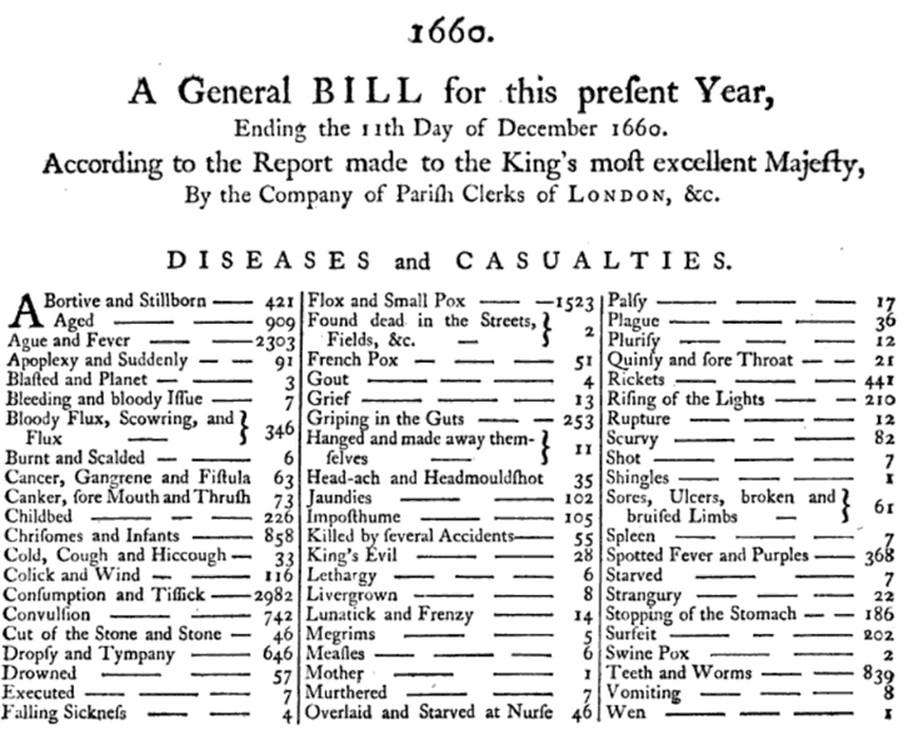
\includegraphics[width=1\linewidth]{images/StandardizedVocabularies/bill} 

}

\caption{1660 London Bill of Mortality, 당시 알려진 62가지 질병의 분류 체계를 사용하여 사망한 거주자의 사망 원인을 보여준다.}\label{fig:bill}
\end{figure}

그 후, 의학 용어 분류는 규모와 복잡성이 크게 확대되면서 시술, 서비스,
약물, 의료기기 등, 의료의 다른 측면으로 널리 전파되었다. 의학 용어
분류의 주요 원칙은 동일하게 유지된다: 즉, 일부 의료 커뮤니티가 환자
데이터를 획득, 분류 및 분석하기 위한 목적으로 동의한 통제 어휘,
전문용어, 계층 및 언어 concept (ontologies: 온톨로지) 이다. 이러한
용어집의 상당수는 공공기관과 정부 기관에서 장기적으로 의무 관리하고
있다. 예를 들면, 세계보건기구(WHO)는 최근 국제 질병분류(ICD)에 11차
개정판(ICD11)을 추가하였다. 지역 정부들은 ICD10CM(미국), ICD10GM(독일)
등과 같은 국가별 버전을 만들고 있다. 정부들은 또한 의약품의 마케팅과
판매를 통제하고 인증된 의약품의 국가 저장 목록을 운영하고 있다. 용어집은
상업용 제품 또는 내부용으로 민간 부문에서도 사용된다. 예를 들면,
전자건강기록(EHR) 시스템과 의료보험청구용이 있다.

그 결과, 각 국가, 지역, 의료시스템 및 의료기관은 그 용어가 사용되는
지역에서만 쓰이는 자체 질병분류체계를 갖고 있을 가능성이 높다. 이러한
무수히 많은 용어집은 사용 중인 시스템의 상호운용성을 방해한다. 표준화는
환자 데이터 교환을 가능하게 하고, 전 세계적 수준의 의료 데이터 분석의
길을 열어주고, 성능 특성 분석 및 품질 평가를 포함한 체계적이고 표준화된
연구를 가능하게 하는 핵심 요소이다. 이러한 문제를 해결하기 위해, 위에서
언급된 WHO와 the Standard Nomenclature of Medicine(SNOMED) 또는 Logical
Observation Identifiers Names and Codes(LOINC) 같은 다국적 기관들이
생겨나고 광범위한 표준들을 만들기 시작했다. 미국의 보건 IT 표준 위원회
HITAC(Health IT Standards Committee)는 다양한 단체 간의 건강 정보 교환을
위한 공통 플랫폼에서 사용하기 위해 ONC(National Coordinator for Health
IT)의 표준으로 SNOMED, LOINC 및 약물용어인 RxNorm을 사용할 것을 권장하고
있다.

OHDSI는 관찰 연구를 위한 국제 표준인 OMOP CDM을 개발했다. CDM의 일부로,
OMOP 표준 용어는 다음 두 가지 목적으로 사용 할 수 있다:

\begin{itemize}
\tightlist
\item
  커뮤니티에서 사용되는 모든 용어의 공통 저장 자료
\item
  연구에 사용하기 위한 표준화와 매핑
\end{itemize}

표준화된 용어는 커뮤니티에 무료로 제공되며, \textbf{OMOP CDM 실제
사용시마다 필수 참조 테이블로 사용되어야 한다.}

\subsection{표준화된 용어 구축}\label{--}

표준 용어의 모든 용어는 동일한 공통 형식으로 통합된다. 이를 통해
연구자들이 기존 용어의 여러 가지 형식과 수명 주기 규칙을 이해하거나
처리할 필요가 없다. 모든 용어는 Pallas 시스템\footnote{\url{https://github.com/OHDSI/Vocabulary-v5.0}}을
사용하여 정기적으로 새로워지고 통합 된다. 용어는 OMOP CDM Workgroup의
일부인 OHDSI Vocabulary 팀이 만들어 운영하고 있다. 오류가 발견되면 OHDSI
Forums\footnote{\url{https://forums.ohdsi.org}} 또는 CDM Github
페이지\footnote{\url{https://github.com/OHDSI/CommonDataModel/issues}}에
게시하여 오류를 보고하고 리소스를 개선할 수 있도록 도와주길
바란다.\index{Pallas system}

\subsection{표준 용어 이용하기}\label{accessVocabularies}

표준 용어 정보를 얻기 위해, Pallas를 직접 실행할 필요는 없다. 대신,
ATHENA\footnote{\url{http://athena.ohdsi.org}}에서 최신 버전을
다운로드하여 로컬 데이터베이스에 적재하면 된다. ATHENA도 용어를 면밀히
검색하는 기능이 있다. \index{ATHENA}
\index{standardized vocabularies!download}
\index{standardized vocabularies!search}

모든 표준 용어 테이블에 포함된 zip 파일을 다운로드하려면, OMOP CDM에
필요한 모든 용어집을 선택해야 한다. 표준 concept을 가진 용어집은
(\ref{standardConcepts}절 참조) 미리 선택되어 있다. source data에
사용되는 vocabularies를 추가한다. 저작권이 있는 용어집은 선택할 수 없다.
해당 용어집을 리스트에 포함하려면 ``License required'' 버튼을 클릭해야
한다. 용어팀이 당신에게 연락할 것이고, 당신이 라이센스를 제출하도록
요청하거나, 해당 라이센스를 얻는데 적절한 사람들과 연결해줄 것이다.

\subsection{용어의 원천: 도입 vs 구축}\label{---vs-}

OHDSI는 일반적으로 용어집을 새로 구축하기보다는 기존에 사용되는 용어집을
채택하는 것을 선호한다. 왜냐하면 (i) 많은 용어집이 이미 공동체의 관찰
데이터에 사용되어 왔으며 (ii) 용어집의 구성 및 유지 관리가 복잡하여 오랜
기간 동안 많은 이해관계자의 의견을 수렴해야 하기 때문이다. 이러한
이유로, 전담 조직은 생성, 사용 중단, 병합 및 분할의 수명 주기에 따라
용어집을 제공하고 있다. (\ref{conceptLifeCycle}절 참조) 현재 OHDSI는
Type Concepts (예를 들어, condition type concepts)과 같은 내부 관리
용어만 생성하고 있다. 유일한 예외는 RxNorm Extension인데, RxNorm
Extension은 미국 이외의 지역에서만 사용되는 약물 용어집이다.
(\ref{rxNormExtension}절 참조)

\section{Concept}\label{concept}

OMOP CDM의 모든 임상 사건들은 concept으로 표현되며, 이는 각 사건의 의미
있는 concept을 나타낸다. Concept은 데이터 기록들의 기본적인 구성
요소로써, 모든 테이블을 거의 예외 없이 완전 정규화한다. Concept은
CONCEPT table에 저장된다. (그림 \ref{fig:concept} 참조) \index{concept}

\begin{figure}

{\centering 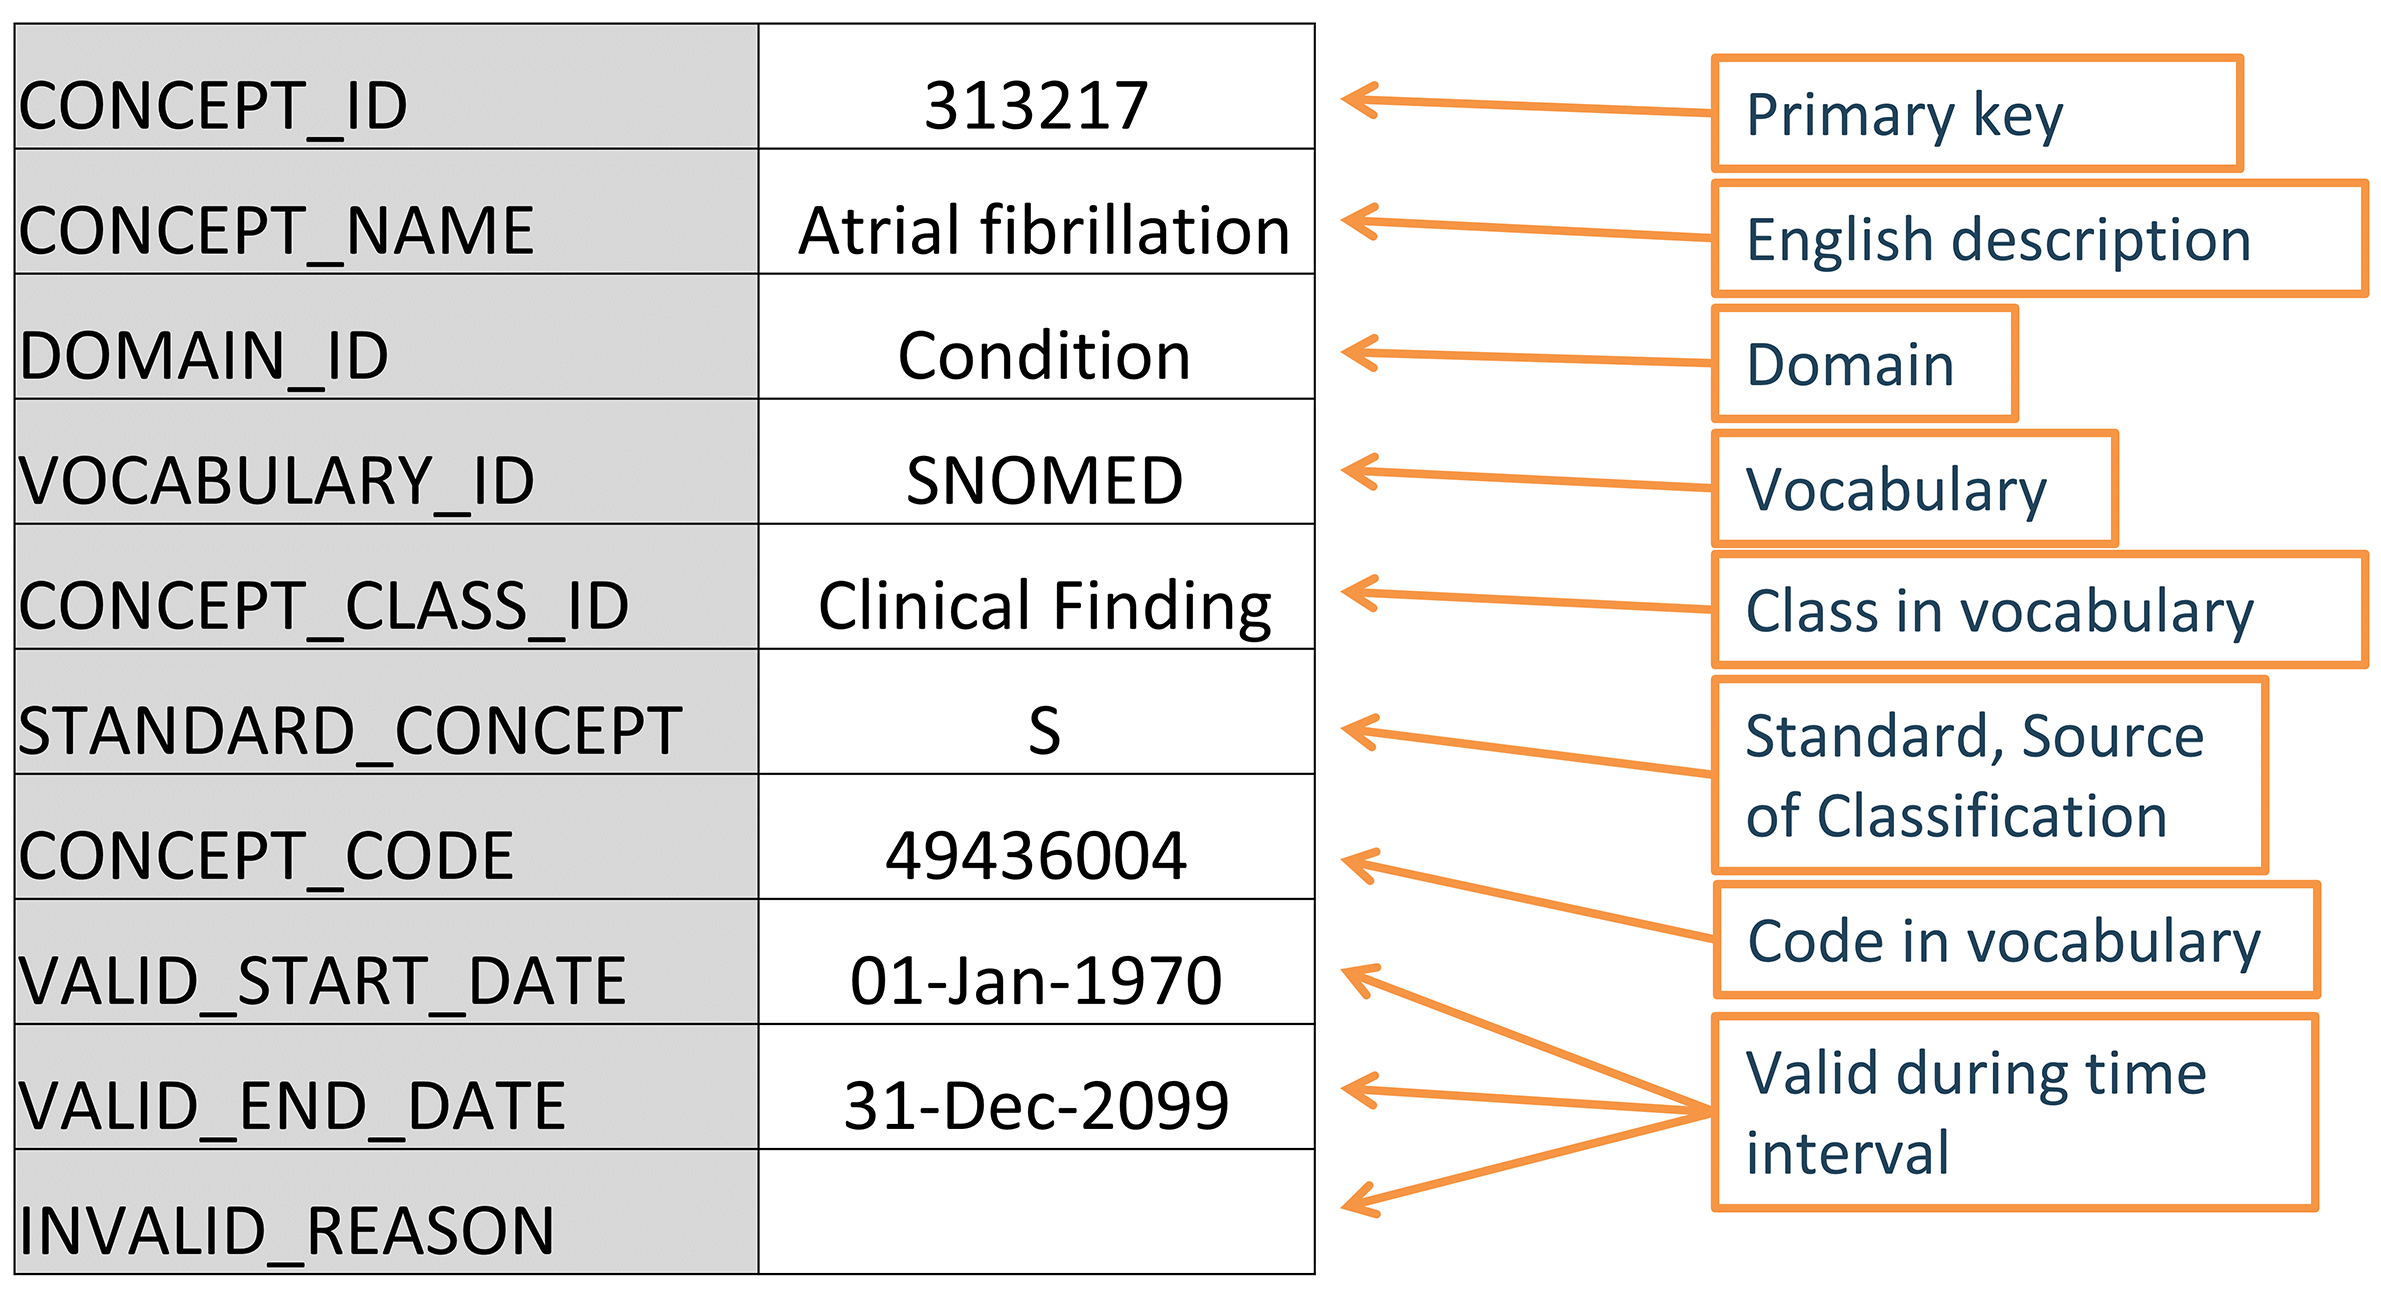
\includegraphics[width=0.9\linewidth]{images/StandardizedVocabularies/concept} 

}

\caption{OMOP CDM에서 vocabulary의 표준 표현. 위의 예는 심방세동의 SNOMED 코드에 대한 CONCEPT 테이블 레코드이다.}\label{fig:concept}
\end{figure}

이 시스템은 포괄적이지 않으면 안 된다. 즉, 환자의 의료 경험 (예를 들어,
진단명, 시술, 약물 노출 등) 및 의료시스템의 일부 관리 정보 (예를 들어,
병원 방문, 관리 부위 등) 과 관련된 모든 이벤트를 포괄할 만큼 충분히 많은
concept이 있어야 한다.

\subsection{Concept IDs}\label{concept-ids}

각각의 concept ID는 Concept ID를 기본 키로 할당한다. 이 무의미한 정수
ID는, 단어의 원 코드보다는 CDM 이벤트 테이블에 데이터를 기록하는 데
사용된다.

\subsection{Concept 이름}\label{concept-}

각 concept에는 하나의 이름이 있다. 그 이름은 항상 영어로 되어있다.
concept들은 용어집의 source로부터 가져온다. source vocabulary에 둘
이상의 이름을 가지고 있으면, 가장 표현력이 높은 이름이 선택되고, 나머지
이름은 동일한 CONCEPT\_KEY로 CONCEPT\_SYNONYM 테이블에 저장된다. 영어
이외의 이름은 CONCEPT\_SYNONYM에 기록되며, 적합한 language concept ID가
LANGUAGE\_CONCEPT\_ID 필드에 기록된다. 이름은 255자까지의 길이를
가지는데, 너무 긴 이름은 잘라내고 최대 1,000자까지 저장 가능한 다른
이름의 동의어로 기록된다.

\subsection{도메인}\label{conceptDomains}

각 concept에는 DOMAIN\_ID가 필드에 할당되는데, 숫자 CONCEPT\_ID와 달리
도메인의 대소문자를 구분하면서 길이가 짧은 고유한 영 숫자 ID이다. 이러한
각 도메인의 예로는 ``Condition'', ``Drug'', ``Procedure'', ``Visit'',
``Device'', ``Specimen'' 등이 있다. 모호하거나
pre-coordinated(combination) concepts의 경우 combination 도메인에 속할
수 있으나, 표준 concept은 (\ref{standardConcepts}절 참조) 항상 단일
도메인에 할당된다. 도메인은 또한 어떤 임상 사건 또는 임상 속성 등이 어떤
CDM 테이블과 필드에 기록되어야 하는지 알려준다. 도메인 할당은
\href{https://github.com/ohDSI/vocabulary-v5.0}{Pallas} 내에 경험적
지식을 이용한 용어 수집 중에 수행되는 OMOP 고유의 특징이다. Source
vocabularies는 서로 다른 도메인들이 함께 혼재되어 있는 경우가 많으나, 그
정도는 각기 다르다 (그림\ref{fig:domains} 참조). \index{domain!concept}

\begin{figure}

{\centering 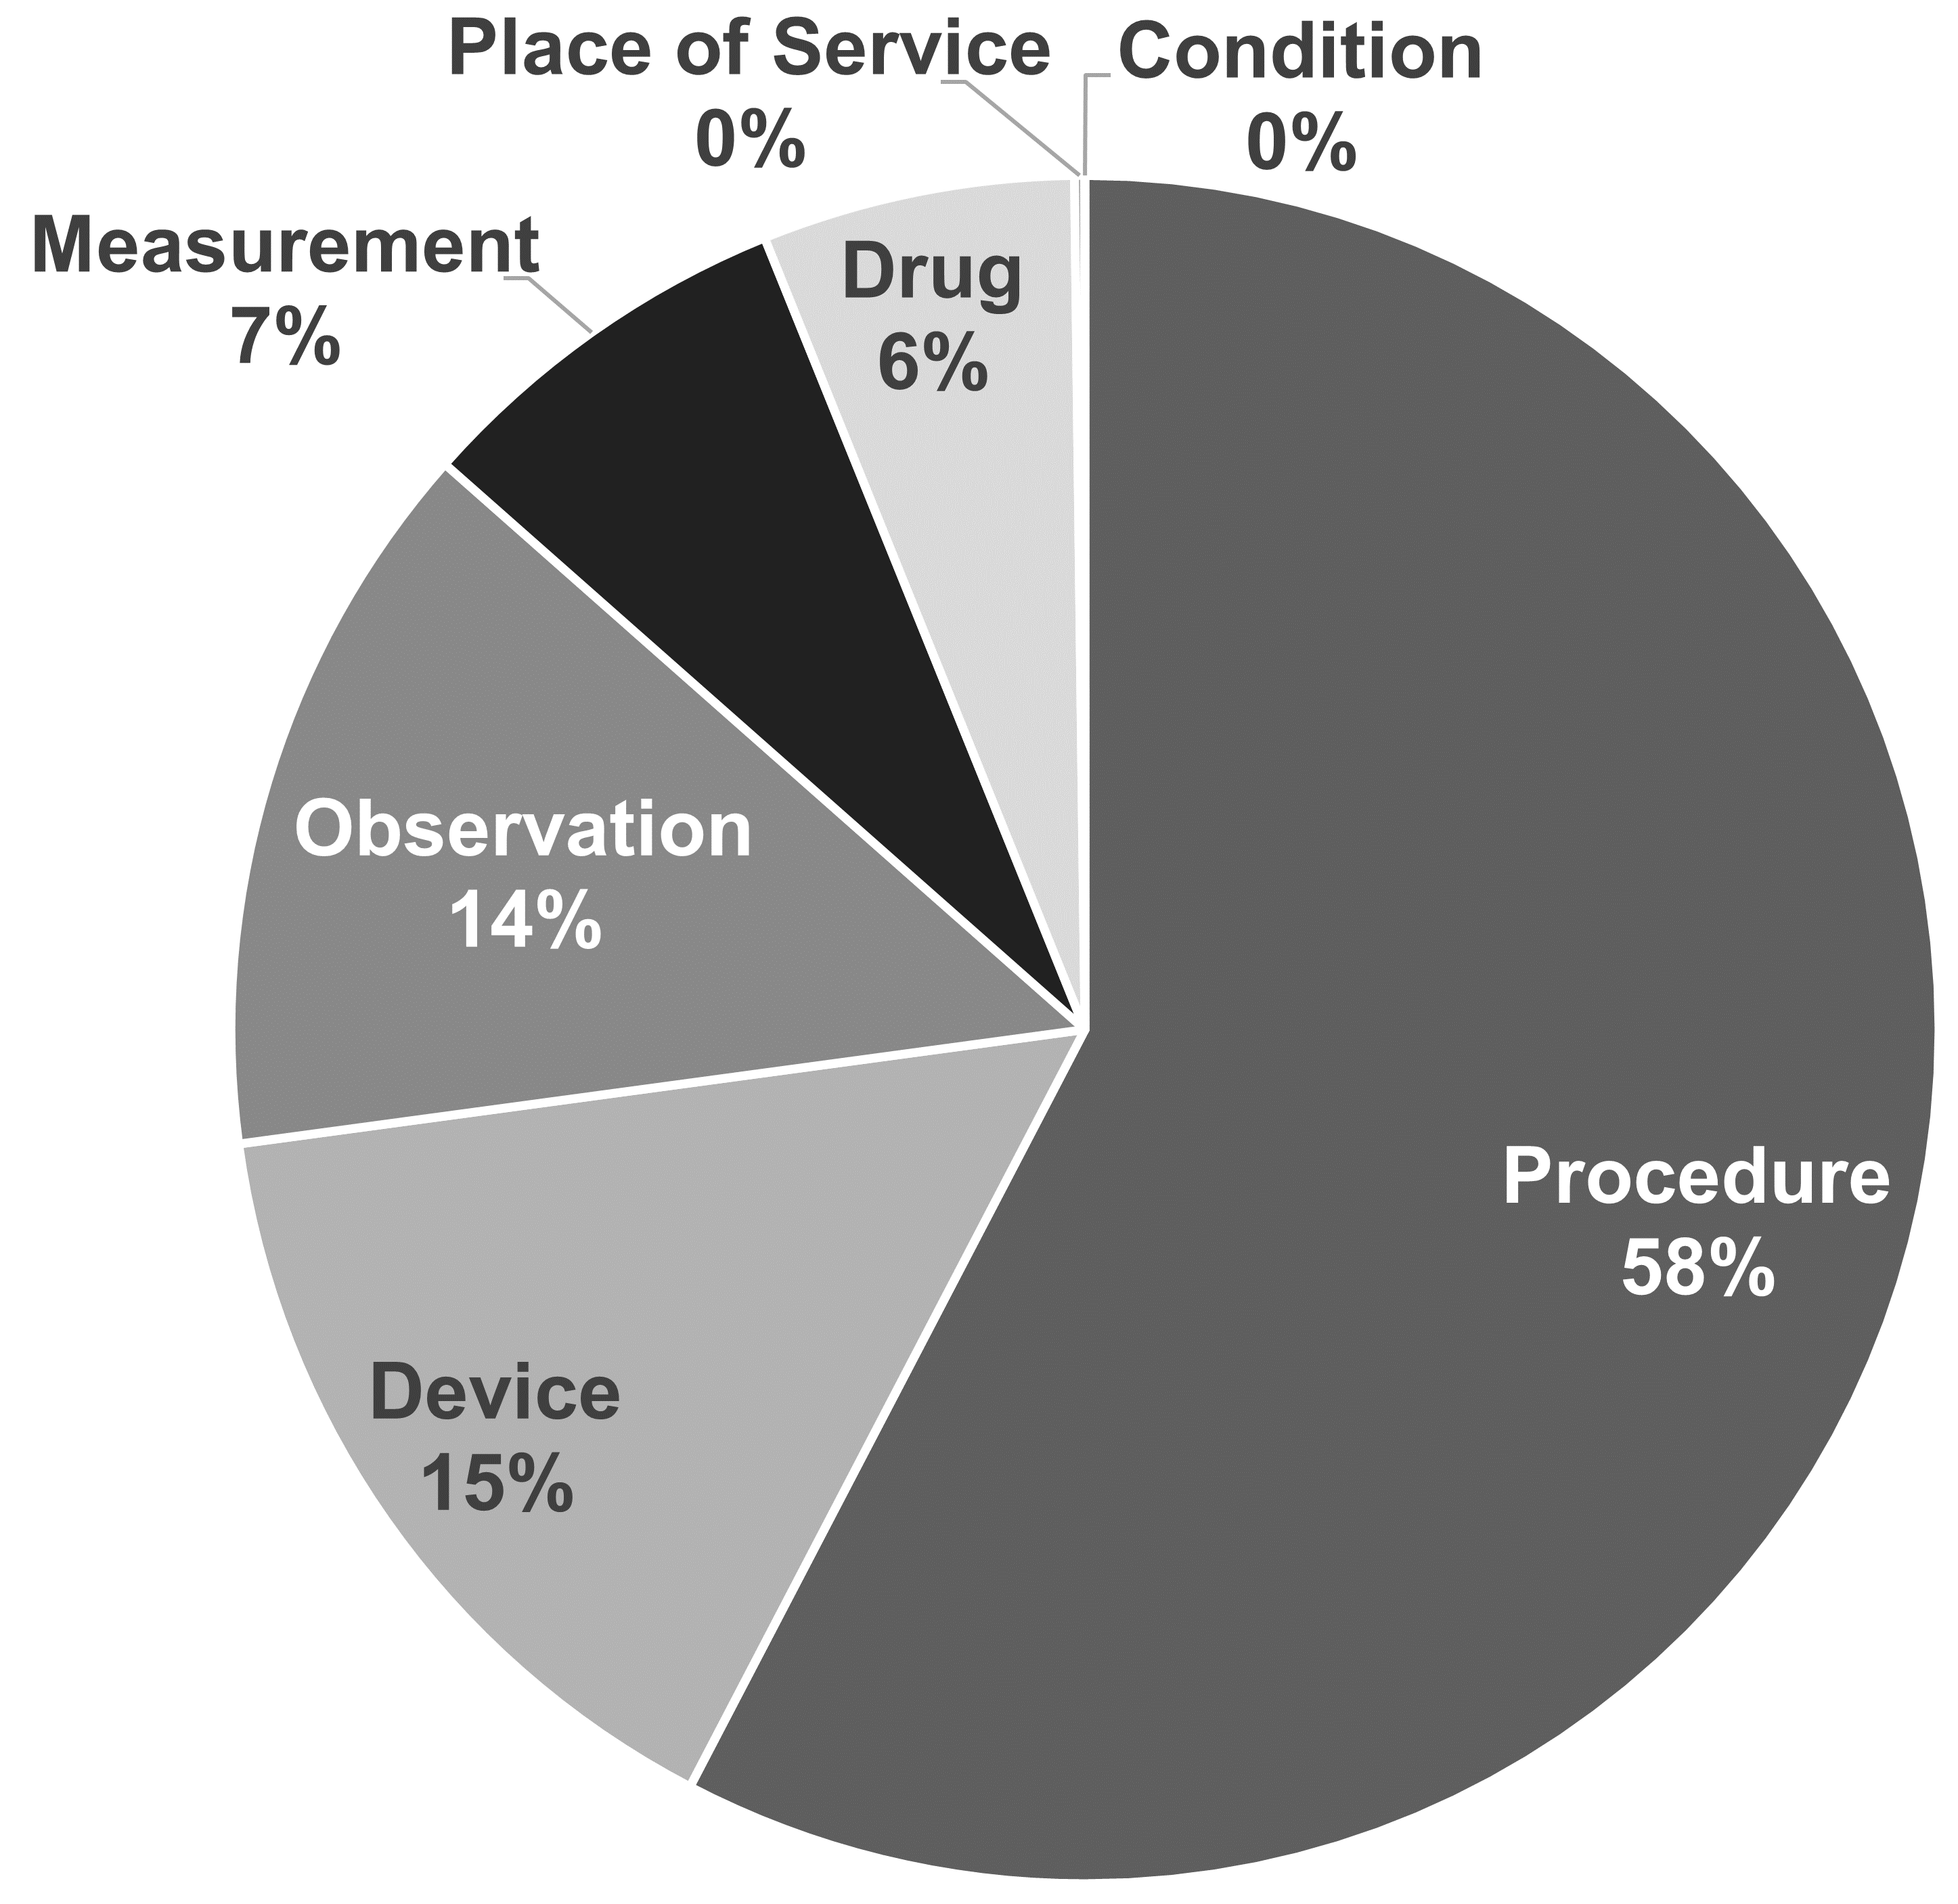
\includegraphics[width=0.7\linewidth]{images/StandardizedVocabularies/domains} 

}

\caption{시술 용어인 CPT4와 HCPCS의 도메인 할당 비율. 직관적으론, 이러한 용어집은 한 도메인의 코드와 concept을 포함하고 있어야 하지만, 실제로는 여러 도메인들이 혼재되어있다.}\label{fig:domains}
\end{figure}

경험적 지식을 이용한 도메인 할당 방법은 도메인의 정의를 따라 진행한다.
이러한 정의는 CDM의 테이블 및 필드 정의에서 파생된다
(\ref{CommonDataModel}장 참조). 경험적 지식은 완벽하지 않으며,
불분명하다 (\ref{specialSituations}절의 ``Special Situations'' 참조).
만일, 잘못 지정된 concept 도메인을 발견한다면,
\href{https://forums.ohdsi.org}{Forums} 또는
\href{https://github.com/OHDSI/CommonDataModel/issues}{CDM issue}
게시판을 통하여, 문제점을 보고하고 개선하도록 해야 한다.

\subsection{용어집 (Vocabularies)}\label{-vocabularies}

각 용어집에는 대소문자를 구분하는 고유한 영 숫자 ID가 있으며, 일반적으로
용어집의 약어 이름을 쓰고, 대시는 생략한다. 예를 들자면, ICD-9-CM의 용어
ID는 ``ICD9CM'' 이다. 현재 OHDSI가 지원하는 용어집은 11개로, 그중 78개가
외부 source에서 채택되었고, 나머지는 OMOP 내부 용어집이다. 이러한 용어는
일반적으로 분기별 일정에 따라 갱신된다. 용어집의 버전은 VOCABULARY
reference file에 따라 정의되어 있다. \index{vocabulary}

\subsection{Concept 계층 (Concept
Classes)}\label{concept--concept-classes}

일부 용어집은 대소문자를 구분하는 고유한 영 숫자 ID를 통해 표현되는
코드나 concept을 분류한다. 예를 들어, SNOMED에는 ``semantic tag''라고
불리는 33가지 concept 계층을 가지고 있다: ``clinical finding'', social
context, body structure 등 concept 계층은 concept들의 수직적 구분을
말한다. MedDRA 또는 RxNorm과 같은 다른 concept들은 계층화된 계급 내에서
수평적인 수준에서 분류하는 concept 계층들을 가지고 있다. HCPCS와 같이
concept 계층이 없는 용어들은 Concept Class ID를 vocabulary ID로 사용해야
한다. \index{concept!class}

\begin{longtable}[]{@{}ll@{}}
\caption{\label{tab:sublassification}concept 계층에서 수평 및 수직 하위분류
원칙에 따른 용어집들}\tabularnewline
\toprule
\begin{minipage}[b]{0.13\columnwidth}\raggedright\strut
Concept class subdivision principle\strut
\end{minipage} & \begin{minipage}[b]{0.47\columnwidth}\raggedright\strut
Vocabulary\strut
\end{minipage}\tabularnewline
\midrule
\endfirsthead
\toprule
\begin{minipage}[b]{0.13\columnwidth}\raggedright\strut
Concept class subdivision principle\strut
\end{minipage} & \begin{minipage}[b]{0.47\columnwidth}\raggedright\strut
Vocabulary\strut
\end{minipage}\tabularnewline
\midrule
\endhead
\begin{minipage}[t]{0.13\columnwidth}\raggedright\strut
Horizontal\strut
\end{minipage} & \begin{minipage}[t]{0.47\columnwidth}\raggedright\strut
all drug vocabularies, ATC, CDТ, Episode, HCPCS, HemOnc, ICDs, MedDRA,
OSM, Census\strut
\end{minipage}\tabularnewline
\begin{minipage}[t]{0.13\columnwidth}\raggedright\strut
Vertical\strut
\end{minipage} & \begin{minipage}[t]{0.47\columnwidth}\raggedright\strut
CIEL, HES Specialty, ICDO3, MeSH, NAACCR, NDFRT, OPCS4, PCORNET, Plan,
PPI, Provider, SNOMED, SPL, UCUM\strut
\end{minipage}\tabularnewline
\begin{minipage}[t]{0.13\columnwidth}\raggedright\strut
Mixed\strut
\end{minipage} & \begin{minipage}[t]{0.47\columnwidth}\raggedright\strut
CPT4, ISBT, LOINC\strut
\end{minipage}\tabularnewline
\begin{minipage}[t]{0.13\columnwidth}\raggedright\strut
None\strut
\end{minipage} & \begin{minipage}[t]{0.47\columnwidth}\raggedright\strut
APC, all Type Concepts, Ethnicity, OXMIS, Race, Revenue Code, Sponsor,
Supplier, UB04s, Visit\strut
\end{minipage}\tabularnewline
\bottomrule
\end{longtable}

수평적 concept 계층을 사용하면 특정 계층 수준을 지정할 수 있게 해준다.
예를 들어, 약물 용어의 RxNorm에서 ``Ingredient'' concept 계층은 최상위층
계급 레벨을 정의한다. 수직적 모델에서 concept 계층 요소들은 최상위에서
맨 아래까지 모든 계급 중의 하나일 수 있다.

\subsection{표준 Concept}\label{standardConcepts}

각 임상 사건의 의미를 나타내는 하나의 concept을 표준 concept(Standard
Concepts)이라고 부른다. 예를 들면, MESH 코드 D001281, CIEL 코드 148203,
SNOMED 코드 49436004, ICD9CM 코드 427.31 및 Read 코드 G573000은 모두
condition 도메인에서 ``심방세동 atrial fibrillation''을 정의하지만,
condition 데이터에서는 SNOMED의 concept만이 표준이고 그 데이터에서
질환을 나타낸다. 나머지는 비표준 concept 또는 원천 concept(source
concepts)으로 지정되고, 표준 concept에 매핑이 된다. 표준 concept은
STANDARD\_CONCEPT 필드에 ``S''라고 표시한다. 그리고 이러한
표준concept만이 ``\_CONCEPT\_ID``로 끝나는 CDM 필드에 데이터를 기록하는
데 사용된다. \index{standard concept}

\subsection{비표준 Concept}\label{-concept}

비표준 concept(Non-Standard Concepts)은 임상사건을 나타내는데 사용되지
않으나, 여전히 표준 용어집의 일부를 구성하고 소스데이터에서 흔히
발견된다. 이런 이유로, 그것들은 ``source concepts''라고 부른다. source
concepts을 표준 concept으로 변환하는 과정을 ``매핑 mapping''이라고
부른다 (\ref{conceptMapping}절 참조). 비표준 concept은 STANDARD\_CONCEPT
필드에 값이 없다(NULL).

\subsection{분류 Concept}\label{-concept}

분류 concept(Classification Concepts)은 표준이 아니므로 데이터를
나타내는데 사용할 수 없다. 하지만 표준 concept과 어울러져 계층 구조를
나타냄으로서, 계층 쿼리(hierarchical queries)를 수행하는데 사용할 수
있다. 예를 들어, MedDRA 코드 10037908의 모든 하위 항목에 대한 쿼리를
사용하면 (MedDRA license를 받지 않는 사용자에게는 보이지 않음,
\ref{accessVocabularies}절 액세스 제한 참조) 심방세동 atrial
Fibrillation에 대한 표준 SNOMED concept이 검색된다. (CONCEPT\_ANCESTOR
테이블을 사용한 계층 쿼리는 \ref{conceptAncestor}절 참조) - 그림
\ref{fig:hierarchy} 참조. \index{classification concept}

\begin{figure}

{\centering 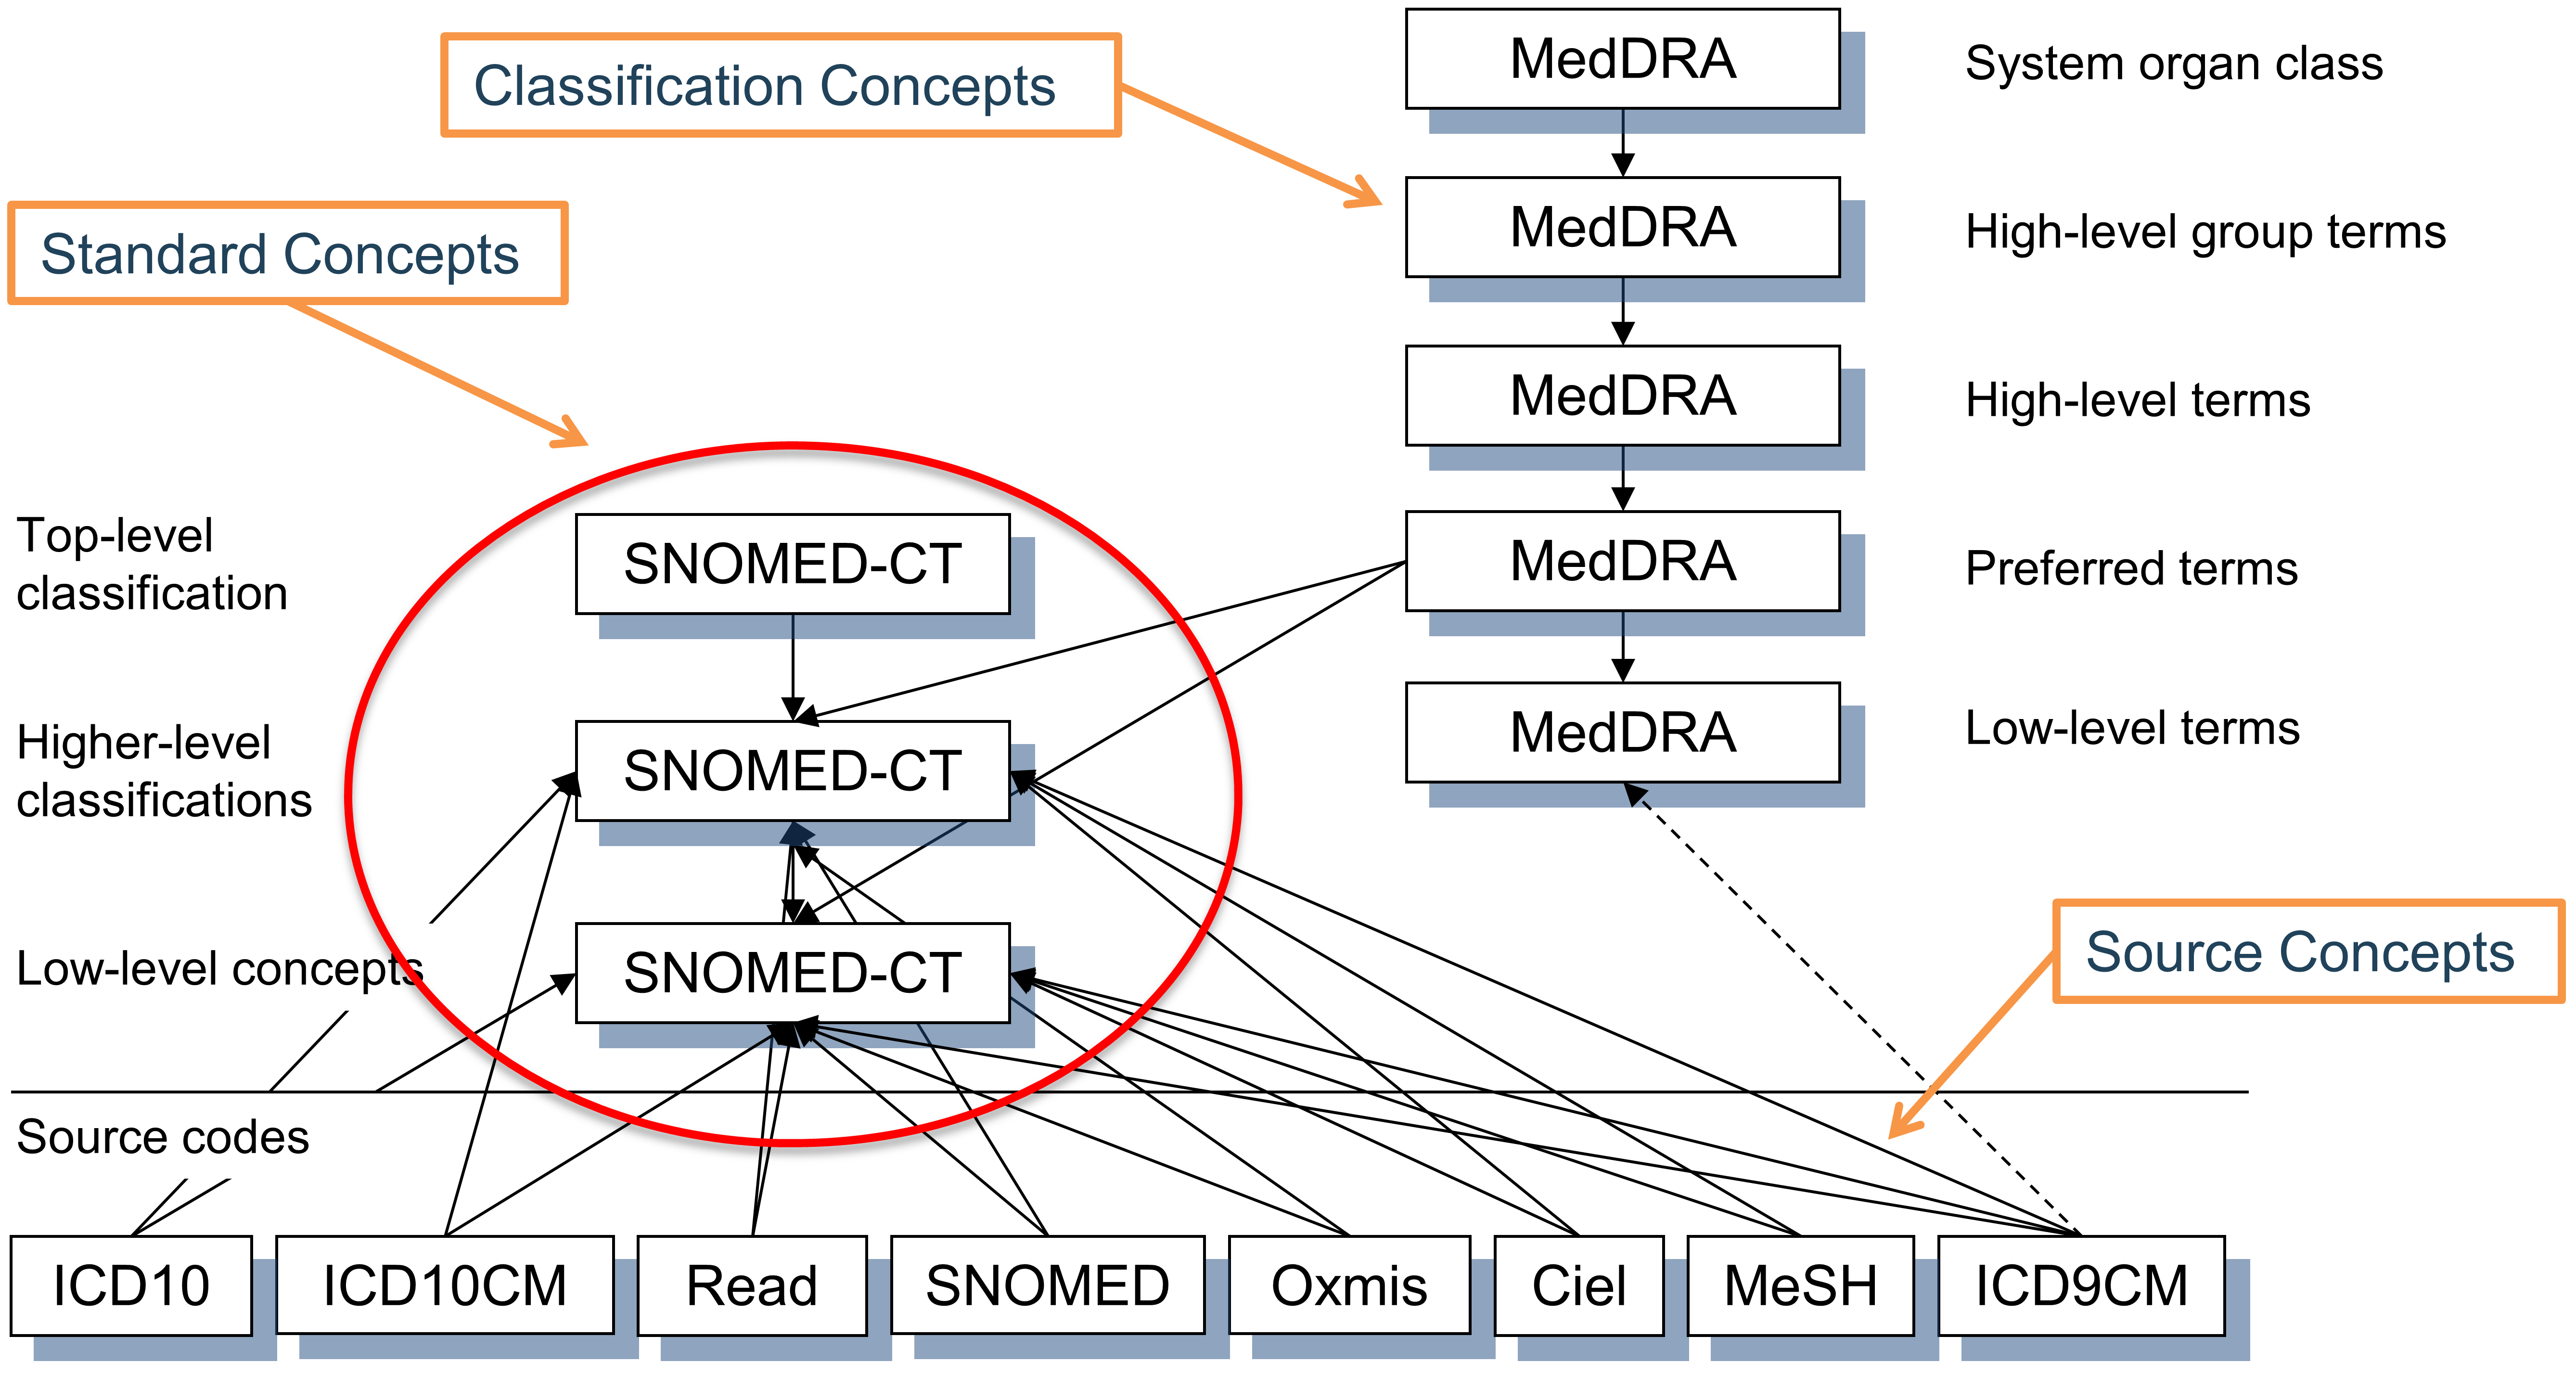
\includegraphics[width=1\linewidth]{images/StandardizedVocabularies/hierarchy} 

}

\caption{Standard, non-standard source 및 분류 concept 및 condition 도메인에서의 계층적 관계. SNOMED는 대부분 standard condition concepts (일부 ICDO3에서 파생된 종양학 관련 concept) 에 사용되고, MedDRA concept은 계층 분류 concept에 사용되며, 그 외 다른 모든 용어집은 비표준 concept이나 혹은 계층 구조에 포함되지 않는 원천 concept을 가지고 있다.}\label{fig:hierarchy}
\end{figure}

concept을 표준, 비표준 및 분류 concept 중 어디로 지정할지 선택할 때, 각
도메인 용어 수준에서 개별적으로 시행한다. 이는 concept의 질, 내장된
계층구조 및 그 용어가 선언된 목적에 따라 행해진다. 또한, 한 용어집의
모든 concept이 표준 concept으로 사용되는 것은 아니다. 어디로 지정할지는
각 도메인마다 분리되어 있고, 각 concept은 유효해야 하며
(\ref{conceptLifeCycle}절 참조), 다른 용어집에서 하나 이상의 concept이
같은 의미로 경쟁하는 경우 우선순위가 있을 수 있다. 다른 말로 하면, 그런
경우에는 표준 용어집은 존재하지 않는다. 예는 표 \ref{tab:vocabList}를
참고하기 바란다.

\begin{longtable}[]{@{}llll@{}}
\caption{\label{tab:vocabList} 표준, 비표준 및 분류 concept 할당에 활용할
용어집 목록}\tabularnewline
\toprule
\begin{minipage}[b]{0.12\columnwidth}\raggedright\strut
도메인\strut
\end{minipage} & \begin{minipage}[b]{0.21\columnwidth}\raggedright\strut
표준 concept\strut
\end{minipage} & \begin{minipage}[b]{0.21\columnwidth}\raggedright\strut
원천 concept\strut
\end{minipage} & \begin{minipage}[b]{0.18\columnwidth}\raggedright\strut
분류 concept\strut
\end{minipage}\tabularnewline
\midrule
\endfirsthead
\toprule
\begin{minipage}[b]{0.12\columnwidth}\raggedright\strut
도메인\strut
\end{minipage} & \begin{minipage}[b]{0.21\columnwidth}\raggedright\strut
표준 concept\strut
\end{minipage} & \begin{minipage}[b]{0.21\columnwidth}\raggedright\strut
원천 concept\strut
\end{minipage} & \begin{minipage}[b]{0.18\columnwidth}\raggedright\strut
분류 concept\strut
\end{minipage}\tabularnewline
\midrule
\endhead
\begin{minipage}[t]{0.12\columnwidth}\raggedright\strut
Condition\strut
\end{minipage} & \begin{minipage}[t]{0.21\columnwidth}\raggedright\strut
SNOMED, ICDO3\strut
\end{minipage} & \begin{minipage}[t]{0.21\columnwidth}\raggedright\strut
SNOMED Veterinary\strut
\end{minipage} & \begin{minipage}[t]{0.18\columnwidth}\raggedright\strut
MedDRA\strut
\end{minipage}\tabularnewline
\begin{minipage}[t]{0.12\columnwidth}\raggedright\strut
Procedure\strut
\end{minipage} & \begin{minipage}[t]{0.21\columnwidth}\raggedright\strut
SNOMED, CPT4, HCPCS, ICD10PCS, ICD9Proc, OPCS4\strut
\end{minipage} & \begin{minipage}[t]{0.21\columnwidth}\raggedright\strut
SNOMED Veterinary, HemOnc, NAACCR\strut
\end{minipage} & \begin{minipage}[t]{0.18\columnwidth}\raggedright\strut
현재까지 없음\strut
\end{minipage}\tabularnewline
\begin{minipage}[t]{0.12\columnwidth}\raggedright\strut
Measurement\strut
\end{minipage} & \begin{minipage}[t]{0.21\columnwidth}\raggedright\strut
SNOMED, LOINC\strut
\end{minipage} & \begin{minipage}[t]{0.21\columnwidth}\raggedright\strut
SNOMED Veterinary, NAACCR, CPT4, HCPCS, OPCS4, PPI\strut
\end{minipage} & \begin{minipage}[t]{0.18\columnwidth}\raggedright\strut
현재까지 없음\strut
\end{minipage}\tabularnewline
\begin{minipage}[t]{0.12\columnwidth}\raggedright\strut
Drug\strut
\end{minipage} & \begin{minipage}[t]{0.21\columnwidth}\raggedright\strut
RxNorm, RxNorm Extension, CVX\strut
\end{minipage} & \begin{minipage}[t]{0.21\columnwidth}\raggedright\strut
HCPCS, CPT4, HemOnc, NAAACCR\strut
\end{minipage} & \begin{minipage}[t]{0.18\columnwidth}\raggedright\strut
ATC\strut
\end{minipage}\tabularnewline
\begin{minipage}[t]{0.12\columnwidth}\raggedright\strut
Device\strut
\end{minipage} & \begin{minipage}[t]{0.21\columnwidth}\raggedright\strut
SNOMED\strut
\end{minipage} & \begin{minipage}[t]{0.21\columnwidth}\raggedright\strut
Others, currently not normalized\strut
\end{minipage} & \begin{minipage}[t]{0.18\columnwidth}\raggedright\strut
현재까지 없음\strut
\end{minipage}\tabularnewline
\begin{minipage}[t]{0.12\columnwidth}\raggedright\strut
Observation\strut
\end{minipage} & \begin{minipage}[t]{0.21\columnwidth}\raggedright\strut
SNOMED\strut
\end{minipage} & \begin{minipage}[t]{0.21\columnwidth}\raggedright\strut
Others\strut
\end{minipage} & \begin{minipage}[t]{0.18\columnwidth}\raggedright\strut
현재까지 없음\strut
\end{minipage}\tabularnewline
\begin{minipage}[t]{0.12\columnwidth}\raggedright\strut
Visit\strut
\end{minipage} & \begin{minipage}[t]{0.21\columnwidth}\raggedright\strut
CMS Place of Service, ABMT, NUCC\strut
\end{minipage} & \begin{minipage}[t]{0.21\columnwidth}\raggedright\strut
SNOMED, HCPCS, CPT4, UB04\strut
\end{minipage} & \begin{minipage}[t]{0.18\columnwidth}\raggedright\strut
현재까지 없음\strut
\end{minipage}\tabularnewline
\bottomrule
\end{longtable}

\subsection{Concept 코드}\label{concept-}

concept 코드(Concept Codes)는 원천 용어집 내에서 사용하는 식별자이다.
예를 들어, ICD9CM 또는 NDC 코드는 해당 필드(concept 코드)에 저장되는데,
OMOP 테이블은 concept ID를 CONCEPT 테이블에 foreign key로 사용을 한다.
그 이유는, 네임 스페이스가 용어집에 걸쳐 겹치기 때문이고, 동일한 코드가
완전히 다른 의미로 다른 용어에 존재할 수 있기 때문이다. (역자 주:
concept 코드는 한 용어집 내에서 유일한 코드로 사용되지만, 같은 코드가
다른 용어집에서 나타날 수 있으나 다른 의미로 사용될 수 있다) (표
\ref{tab:code1001}참조) \index{concept!code}

\begin{longtable}[]{@{}llllll@{}}
\caption{\label{tab:code1001} 같은 concept 코드 1001이 다른 용어집에서 다른
도메인, 다른 concept classes로 사용된다.}\tabularnewline
\toprule
\begin{minipage}[b]{0.13\columnwidth}\raggedright\strut
Concept ID\strut
\end{minipage} & \begin{minipage}[b]{0.07\columnwidth}\raggedright\strut
Concept Code\strut
\end{minipage} & \begin{minipage}[b]{0.16\columnwidth}\raggedright\strut
Concept Name\strut
\end{minipage} & \begin{minipage}[b]{0.14\columnwidth}\raggedright\strut
Domain ID\strut
\end{minipage} & \begin{minipage}[b]{0.14\columnwidth}\raggedright\strut
Vocabulary ID\strut
\end{minipage} & \begin{minipage}[b]{0.14\columnwidth}\raggedright\strut
Concept Class\strut
\end{minipage}\tabularnewline
\midrule
\endfirsthead
\toprule
\begin{minipage}[b]{0.13\columnwidth}\raggedright\strut
Concept ID\strut
\end{minipage} & \begin{minipage}[b]{0.07\columnwidth}\raggedright\strut
Concept Code\strut
\end{minipage} & \begin{minipage}[b]{0.16\columnwidth}\raggedright\strut
Concept Name\strut
\end{minipage} & \begin{minipage}[b]{0.14\columnwidth}\raggedright\strut
Domain ID\strut
\end{minipage} & \begin{minipage}[b]{0.14\columnwidth}\raggedright\strut
Vocabulary ID\strut
\end{minipage} & \begin{minipage}[b]{0.14\columnwidth}\raggedright\strut
Concept Class\strut
\end{minipage}\tabularnewline
\midrule
\endhead
\begin{minipage}[t]{0.13\columnwidth}\raggedright\strut
35803438\strut
\end{minipage} & \begin{minipage}[t]{0.07\columnwidth}\raggedright\strut
1001\strut
\end{minipage} & \begin{minipage}[t]{0.16\columnwidth}\raggedright\strut
Granulocyte colony-stimulating factors\strut
\end{minipage} & \begin{minipage}[t]{0.14\columnwidth}\raggedright\strut
Drug\strut
\end{minipage} & \begin{minipage}[t]{0.14\columnwidth}\raggedright\strut
HemOnc\strut
\end{minipage} & \begin{minipage}[t]{0.14\columnwidth}\raggedright\strut
Component Class\strut
\end{minipage}\tabularnewline
\begin{minipage}[t]{0.13\columnwidth}\raggedright\strut
35942070\strut
\end{minipage} & \begin{minipage}[t]{0.07\columnwidth}\raggedright\strut
1001\strut
\end{minipage} & \begin{minipage}[t]{0.16\columnwidth}\raggedright\strut
AJCC TNM Clin T\strut
\end{minipage} & \begin{minipage}[t]{0.14\columnwidth}\raggedright\strut
Measurement\strut
\end{minipage} & \begin{minipage}[t]{0.14\columnwidth}\raggedright\strut
NAACCR\strut
\end{minipage} & \begin{minipage}[t]{0.14\columnwidth}\raggedright\strut
NAACCR Variable\strut
\end{minipage}\tabularnewline
\begin{minipage}[t]{0.13\columnwidth}\raggedright\strut
1036059\strut
\end{minipage} & \begin{minipage}[t]{0.07\columnwidth}\raggedright\strut
1001\strut
\end{minipage} & \begin{minipage}[t]{0.16\columnwidth}\raggedright\strut
Antipyrine\strut
\end{minipage} & \begin{minipage}[t]{0.14\columnwidth}\raggedright\strut
Drug\strut
\end{minipage} & \begin{minipage}[t]{0.14\columnwidth}\raggedright\strut
RxNorm\strut
\end{minipage} & \begin{minipage}[t]{0.14\columnwidth}\raggedright\strut
Ingredient\strut
\end{minipage}\tabularnewline
\begin{minipage}[t]{0.13\columnwidth}\raggedright\strut
38003544\strut
\end{minipage} & \begin{minipage}[t]{0.07\columnwidth}\raggedright\strut
1001\strut
\end{minipage} & \begin{minipage}[t]{0.16\columnwidth}\raggedright\strut
Residential Treatment - Psychiatric\strut
\end{minipage} & \begin{minipage}[t]{0.14\columnwidth}\raggedright\strut
Revenue Code\strut
\end{minipage} & \begin{minipage}[t]{0.14\columnwidth}\raggedright\strut
Revenue Code\strut
\end{minipage} & \begin{minipage}[t]{0.14\columnwidth}\raggedright\strut
Revenue Code\strut
\end{minipage}\tabularnewline
\begin{minipage}[t]{0.13\columnwidth}\raggedright\strut
43228317\strut
\end{minipage} & \begin{minipage}[t]{0.07\columnwidth}\raggedright\strut
1001\strut
\end{minipage} & \begin{minipage}[t]{0.16\columnwidth}\raggedright\strut
Aceprometazine maleate\strut
\end{minipage} & \begin{minipage}[t]{0.14\columnwidth}\raggedright\strut
Drug\strut
\end{minipage} & \begin{minipage}[t]{0.14\columnwidth}\raggedright\strut
BDPM\strut
\end{minipage} & \begin{minipage}[t]{0.14\columnwidth}\raggedright\strut
Ingredient\strut
\end{minipage}\tabularnewline
\begin{minipage}[t]{0.13\columnwidth}\raggedright\strut
45417187\strut
\end{minipage} & \begin{minipage}[t]{0.07\columnwidth}\raggedright\strut
1001\strut
\end{minipage} & \begin{minipage}[t]{0.16\columnwidth}\raggedright\strut
Brompheniramine Maleate, 10 mg/mL injectable solution\strut
\end{minipage} & \begin{minipage}[t]{0.14\columnwidth}\raggedright\strut
Drug\strut
\end{minipage} & \begin{minipage}[t]{0.14\columnwidth}\raggedright\strut
Multum\strut
\end{minipage} & \begin{minipage}[t]{0.14\columnwidth}\raggedright\strut
Multum\strut
\end{minipage}\tabularnewline
\begin{minipage}[t]{0.13\columnwidth}\raggedright\strut
45912144\strut
\end{minipage} & \begin{minipage}[t]{0.07\columnwidth}\raggedright\strut
1001\strut
\end{minipage} & \begin{minipage}[t]{0.16\columnwidth}\raggedright\strut
Serum\strut
\end{minipage} & \begin{minipage}[t]{0.14\columnwidth}\raggedright\strut
Specimen\strut
\end{minipage} & \begin{minipage}[t]{0.14\columnwidth}\raggedright\strut
CIEL\strut
\end{minipage} & \begin{minipage}[t]{0.14\columnwidth}\raggedright\strut
Specimen\strut
\end{minipage}\tabularnewline
\bottomrule
\end{longtable}

\subsection{수명 주기}\label{conceptLifeCycle}

용어집이 영원불변의 고정된 코드 세트인 경우는 드물다. 오히려, 코드와
concept이 더해지며 꾸준히 수정된다. OMOP CDM은 장기에 걸친 환자 데이터를
지원하기 위한 모델이므로, 과거에 사용되었지만, 지금은 더 이상 사용되지
않는 concept들을 지원해야 할 뿐 아니라, 신설된 concept을 더하여 상황에
맞게 지원해야 한다. CONCEPT 테이블에는 사용 가능한 수명 주기 상태를
설명하는 세 개의 필드가 있다: VALID\_START\_DATE, VALID\_END\_DATE,
INVALID\_REASON 그 값들은 각 concept의 수명 주기 상태에 따라 달라진다.

\begin{itemize}
\tightlist
\item
  \textbf{유효한 concept 및 새로운 concept}

  \begin{itemize}
  \tightlist
  \item
    설명: 사용 중인 concept.
  \item
    VALID\_START\_DATE: concept이 사용되기 시작한 날, 용어집에 concept을
    통합한 날을 알지 못하거나, 알려지지 않은 경우 1970-1-1.
  \item
    VALID\_END\_DATE: ``지금은 활성화되어 있으나, 추후에는 무효가 될
    수가 있음.''을 나타내는 규칙으로 2099-12-31을 설정.
  \item
    INVALID\_REASON: NULL
  \end{itemize}
\item
  \textbf{후속 코드 없이 더 이상 사용되지 않는 concept}

  \begin{itemize}
  \tightlist
  \item
    설명: concept이 비활성화 상태여서 표준으로 사용할 수 없다.
    (\ref{standardConcepts}절 참조)
  \item
    VALID\_START\_DATE: concept이 사용되기 시작한 날, 용어집에 concept을
    통합한 날을 알지 못하거나, 알려지지 않은 경우 1970-1-1.
  \item
    VALID\_END\_DATE: 사용 중단을 나타내는 과거의 날짜, 또는 해당 날짜를
    알 수 없는 경우, concept이 누락되거나 비활성화된 용어집 갱신일
  \item
    INVALID\_REASON: ``D''
  \end{itemize}
\item
  \textbf{후속 코드가 있는 업그레이드 된 concept}

  \begin{itemize}
  \tightlist
  \item
    설명: 비활성이지만, 후속 코드가 정의된 concept. 이들은 일반적으로
    중복 제거를 통해 제거된 concept.
  \item
    VALID\_START\_DATE: concept이 사용되기 시작한 날, 용어집에 concept을
    통합한 날을 알지 못하거나, 알려지지 않은 경우 1970-1-1.
  \item
    VALID\_END\_DATE: 업그레이드를 나타내는 과거의 날짜, 또는 해당
    날짜를 알 수 없는 경우, 업그레이드가 추가된 용어집 갱신일
  \item
    INVALID\_REASON: ``U''
  \end{itemize}
\item
  \textbf{다른 새로운 concept에 대한 재사용 코드}

  \begin{itemize}
  \tightlist
  \item
    설명: 용어집은 새로운 concept을 위해 없어진 concept의 concept 코드를
    재사용했다.
  \item
    VALID\_START\_DATE: concept이 사용되기 시작한 날, 용어집에 concept을
    통합한 날을 알지 못하거나, 알려지지 않은 경우 1970-1-1.\\
  \item
    VALID\_END\_DATE: 사용 중단을 나타내는 과거의 날짜, 또는 해당 날짜를
    알 수 없는 경우, concept이 누락되거나 비활성화로 설정된 용어집
    갱신일
  \item
    INVALID\_REASON: ``R''
  \end{itemize}
\end{itemize}

일반적으로 concept 코드는 재사용하지 않는다. 하지만 이 규칙에서 벗어나는
몇몇 용어집으로 HCPCS, NDC, DRG가 있다. 그들 용어집에서는 동일한 concept
코드가 같은 용어집 내에서 하나 이상의 concept에 사용된다. 그들의
CONCEPT\_ID 값은 고유값을 유지한다. 재사용된 concept 코드는
INVALID\_REASON 필드에 ``R''로 표시되며 VALID\_START\_DATE 부터
VALID\_END\_DATE 까지의 기간을 이용하여 concept 코드는 같지만 서로 다른
concept을 구별하는데 사용해야 한다.

\section{관계 Relationships}\label{-relationships}

두 concept이 동일한 도메인 또는 용어집에 속하는지 여부와 관계없이 두
concept은 지정된 관계를 맺을 수 있다. 관계의 특성은
CONCPET\_RELATIONSHIP 테이블의 RELATIONSHIP\_ID 필드에서 대소문자를
구분하는 고유한 짧은 영 숫자 ID로 표시한다. 각 관계에 대해서 전후가 바뀐
대칭 관계가 존재하며, CONCEPT\_ID\_1, CONCEPT\_ID\_2 필드의 내용이
교환되고, RELATIONSHIP\_ID는 반대로 바뀌게 된다. 예를 들어, ``Maps to''
관계는 ``Mapped from''과 반대의 관계를 갖는다.
\index{concept!relationship}

CONCEPT\_RELATIONSHIP 테이블 레코드에는 수명 주기 필드인
RELATIONSHIP\_START\_DATE, RELATIONSHIP\_END\_DATE, INVALID\_REASON이
있다. 그러나, INVALID\_REASON = NULL인 유효한 기록들만 ATHENA에서 이용할
수 있다. 비활성화된 관계는 Pallas 시스템 내에서 내부처리 용도로만
사용되도록 보관된다. RELATIONSHIP 테이블은 전체 relationship IDs 목록 및
그 반대의 목록과 함께 참조로 사용된다.

\subsection{매핑 관계 Mapping Relationships}\label{conceptMapping}

이러한 관계는 두 개의 relationship ID 쌍을 이용하여 비표준화 concept에서
표준concept으로 변환 하게 해준다. (표 \ref{tab:mappingRelationships}
참조). \index{concept!mapping}

\begin{longtable}[]{@{}ll@{}}
\caption{\label{tab:mappingRelationships} 매핑관계의 유형.}\tabularnewline
\toprule
\begin{minipage}[b]{0.20\columnwidth}\raggedright\strut
Relationship ID pair\strut
\end{minipage} & \begin{minipage}[b]{0.71\columnwidth}\raggedright\strut
Purpose\strut
\end{minipage}\tabularnewline
\midrule
\endfirsthead
\toprule
\begin{minipage}[b]{0.20\columnwidth}\raggedright\strut
Relationship ID pair\strut
\end{minipage} & \begin{minipage}[b]{0.71\columnwidth}\raggedright\strut
Purpose\strut
\end{minipage}\tabularnewline
\midrule
\endhead
\begin{minipage}[t]{0.20\columnwidth}\raggedright\strut
``Maps to'' and ``Mapped from''\strut
\end{minipage} & \begin{minipage}[t]{0.71\columnwidth}\raggedright\strut
표준 concept에 매핑. 표준 concept은 자기 자신에게 매핑되고, 비표준
concept은 표준 concept으로 매핑된다. 대부분의 비표준 concept과 모든 표준
concept들은 한 표준 concept과 이러한 관계를 맺는다. 비표준 concept은
*\_SOURCE\_CONCEPT\_ID에 저장되고 표준 concept은 * \_CONCEPT\_ID 필드에
저장된다. 분류 concept(Classification concepts)은 매핑되지 않는다.\strut
\end{minipage}\tabularnewline
\begin{minipage}[t]{0.20\columnwidth}\raggedright\strut
``Maps to value'' and ``Value mapped from''\strut
\end{minipage} & \begin{minipage}[t]{0.71\columnwidth}\raggedright\strut
MEASUREMENT와 OBSERVATION 테이블의 VALUE\_AS\_CONCEPT\_ID 필드에 배치할
값을 나타내는 concept에 Mapping.\strut
\end{minipage}\tabularnewline
\bottomrule
\end{longtable}

이러한 매핑 관계를 사용하는 목적은 같은 concept간의 교차를 통해 OMOP
CDM에서 임상 사건이 표현되는 방식을 조화롭게 해주는 것이다. 이는
표준화된 용어들이 이루어 낸 주요 성과이다.

``동등 concept(Equivalent concepts)''은 동일한 의미를 가지며, 중요한
것은 계층적으로 하위 concept(descendant)들이 동일한 의미론적 공간을
가진다. 동등concept을 사용할 수 없고, 그 concept이 표준이 아닌 경우, 그
concept은 약간 더 넓은 의미를 가진 concept으로 (소위,
``uphill-mappings'') 매핑된다. 예를 들어, ICD10CM W61.51 ``Bitten by
goose'' 는 일반적으로 표준 condition concept에 사용되는 SNOMED
용어집에는 없다. 대신 SNOMED 217716004의 ``Peck by bird''에 매핑되지만,
그 새가 거위라는 맥락을 잃게 된다. Up-hill 매핑은 정보가 유실돼도 표준
연구 사례들을 진행하는 데 문제없다고 간주할 때만 사용해야 한다.

일부 매핑은 원천 concept을 둘 이상의 표준 concept에 연결한다. 예를 들어,
ICD9CM의 070.43 ``Hepatitis E with hepatic coma''는 SNOMED의 235867002
``Acute hepatitis E''뿐 아니라 SNOMED의 72836002 ``Hepatic Coma'' 에도
매핑되어 있다. 그 이유는 기존의 원천 concept이 간염 hepatitis와 혼스
coma라는 두 가지 조건의 선 조합 pre-coordinated이기 때문이다. SNOMED에는
해당 조합이 없음으로, ICD9CM 레코드에 기록된 두 개의 레코드 (각각 매핑된
표준 concept이 있는 레코드) 가 생성된다.

``Maps to value'' 관계는 Entity-Attribute-Value(EAV) 모델에 따라 OMOP
CDM 테이블의 값을 나누기 위한 목적이 있다. 일반적으로 다음과 같은
경우이다:

\begin{itemize}
\tightlist
\item
  테스트와 결과값으로 구성된 측정값
\item
  개인 또는 가족의 질병력
\item
  물질에 대한 알레르기
\item
  예방접종 필요
\end{itemize}

이런 상황들에서 source concept은 속성(test or history)과 값(test result
or disease)의 조합이다. ``Maps to'' 관계는 소스를 속성 concept에
매핑하고, ``Maps to value'' 관계는 value concept을 매핑한다. (예로 그림
\ref{fig:conceptValue}참조)

\begin{figure}

{\centering 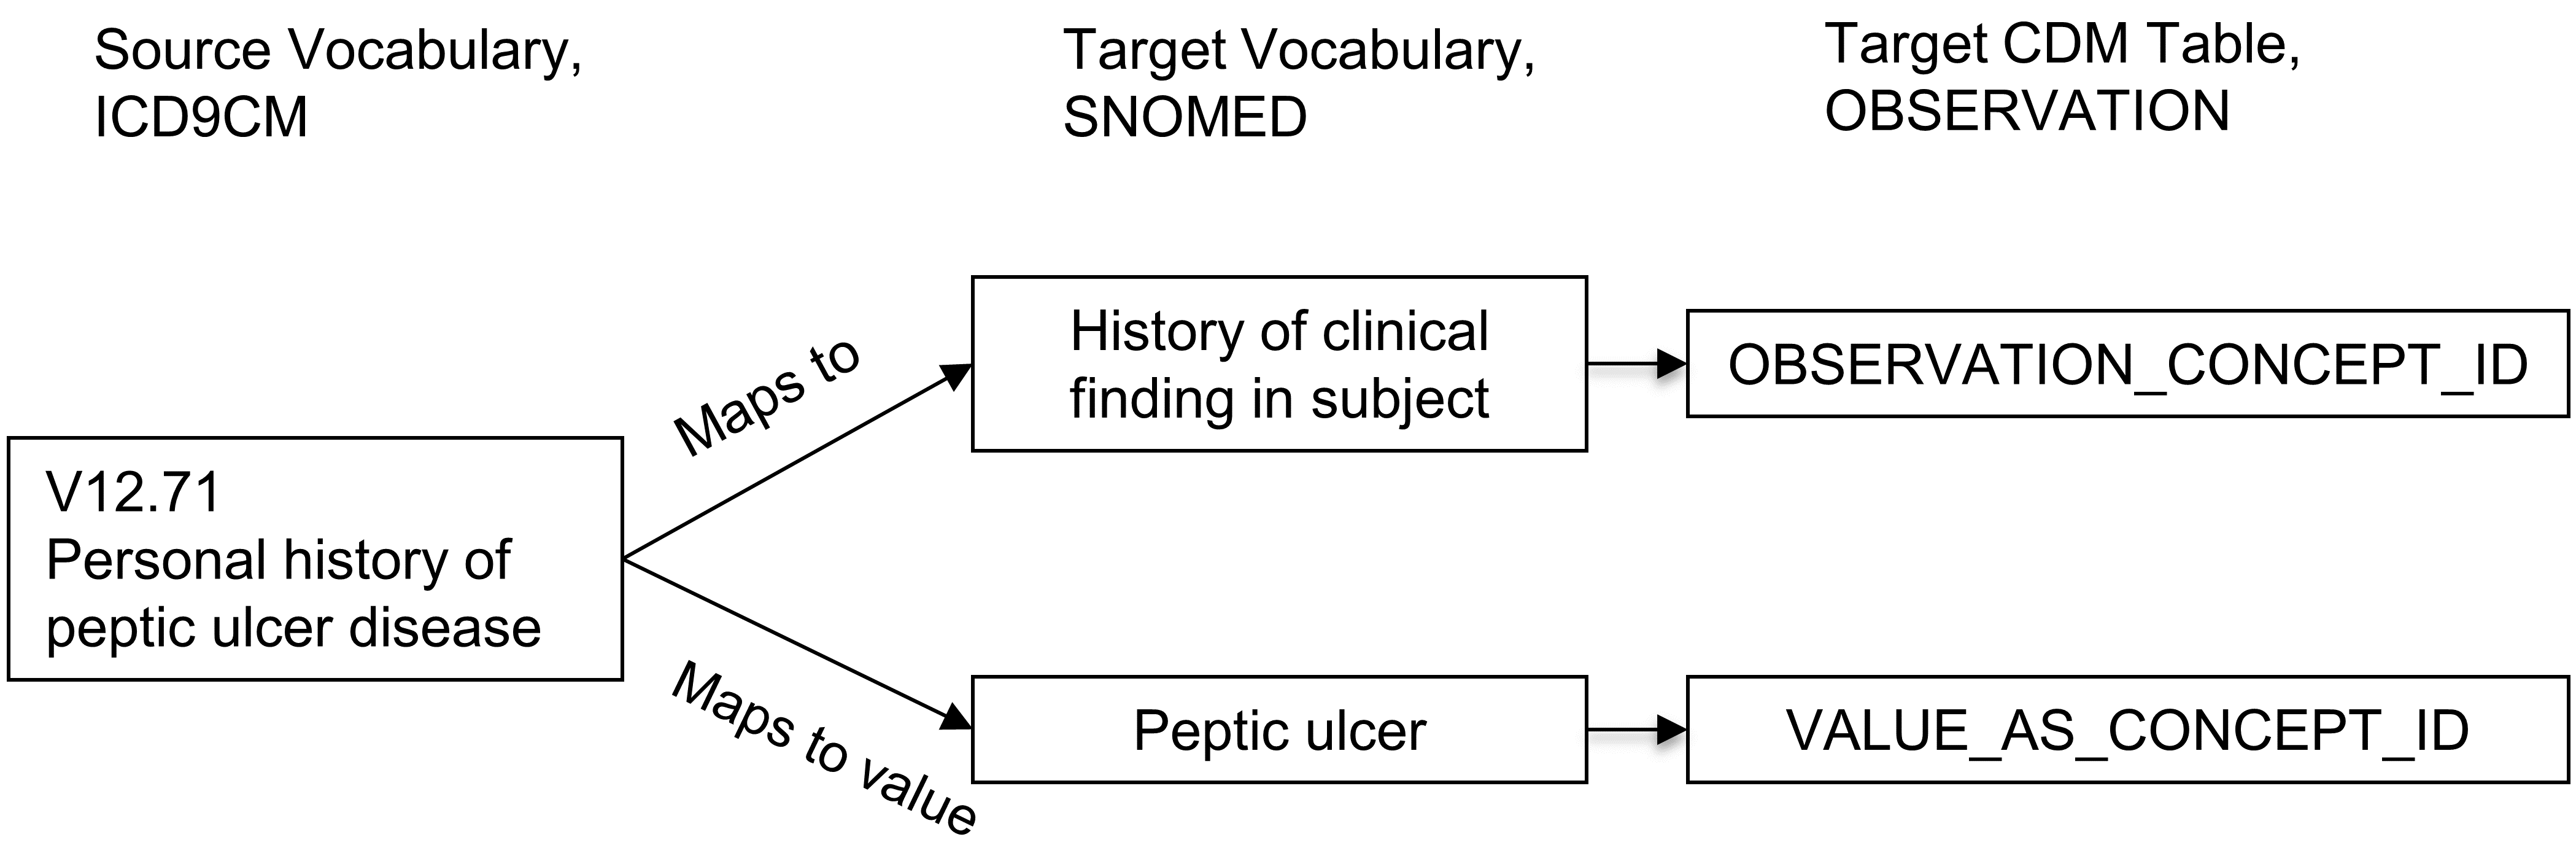
\includegraphics[width=1\linewidth]{images/StandardizedVocabularies/conceptValue} 

}

\caption{원천 concept과 표준 concept 사이의 일대다 매핑. 선 조합 pre-coordinated concept은 두 가지 concept으로 나뉘는데, 하나는 속성(여기서는 임상 소견의 과거력)과 다른 하나는 값(소화성 궤양 peptic ulcer)이다. "Maps to" 관계는 measurement 또는 observation 도메인에 매핑되는 반면, "Maps to value" concept에는 도메인 제한이 없다.}\label{fig:conceptValue}
\end{figure}

concept 매핑은 네트워크 연구를 수행하는 구성원들의 노력을 도와주는
지원과, 무료로 제공되는 OMOP 표준 용어집의 또 다른 핵심 기능이다. 매핑
관계는 외부 소스에서 파생되거나 용어팀에 의해 수작업으로 유지 관리된다.
이것은 용어팀이 완벽하지 않다는 것을 의미한다. 잘못되거나 이의가 있는
매핑 관계를 발견한 경우 \href{https://forums.ohdsi.org}{Forums} 또는
\href{https://github.com/OHDSI/CommonDataModel/issues}{CDM issue}
게시판을 통해 알려줘서 프로세스를 개선하도록 돕는 것이 중요하다.

매핑 규칙에 대한 자세한 설명은 OHDSI Wiki에서 확인할 수 있다. \footnote{\url{https://www.ohdsi.org/web/wiki/doku.php?id=documentation:vocabulary:mapping}}

\subsection{계층적 관계}\label{-}

계층을 나타내는 관계는 ``Is a'' -- ``Subsumes'' 관계를 통해 정의된다.
계층적 관계는 자식 concept이 하나 이상의 추가 속성이나 더욱 정밀하게
정의된 속성에 더하여, 부모 concept의 모든 속성을 갖도록 정의된다. 예를
들어, SNOMED의 49436004 ``심방세동 atrial fibrillation''은 ``Is a''
관계를 통해 SNOMED의 17366009 ``심방 부정맥 atrial arrhythmia''에
연결된다. 두 concept 모두 부정맥arrhythmia 형태를 제외하고 다른 속성은
동일하다, 즉, 한 concept에는 세동 fibrillation으로 정의되고, 다른
concept에서는 세동으로 정의되지 않는다. concept에는 둘 이상의 부모와 둘
이상의 자식 concept이 있을 수 있다. 이 예에서는, SNOMED의 49436004
``심방세동 atrial fibrillation''은 SNOMED의 40593004 ``세동
fibrillation''과도 ``Is-a'' 관계를 가진다. \index{concept!hierarchy}

\subsection{서로 다른 용어집에서 온 concept들 간의
관계}\label{----concept--}

이들 관계는 일반적으로 ``Vocabulary A -- Vocabulary B equivalent''의
유형으로, 기존 용어집 소스에서 제공되거나, OHDSI 용어팀에 의해 구축된다.
그것들은 대략적인 매핑 역할을 할 수 있지만, 종종 잘 정리된 매핑보다는
관계의 정확도가 떨어진다. High-quality equivalence 관교 (예: Source --
RxNorm equivalent) 는 항상 ``Maps to'' 관계에 의해 복제된다.

\subsection{동일 용어집 내 concept들 간의 관계}\label{---concept--}

한 용어집 내부의 관계는 일반적으로 용어집 제공자가 보급한다. 전체적인
설명은 OHDSI Wiki의 개별 용어집 아래의 용어집 설명서에서 찾을 수 있다.
이들 중 다수는 임상 사건 간의 관계를 정의하여 정보 검색에 이용될 수
있다. 예를 들어, 요도 장애 disorders of the urethra는 ``finding site
of'' 관계를 따라가면 찾을 수 있다. (표 \ref{tab:findingSite}참조)

\begin{longtable}[]{@{}ll@{}}
\caption{\label{tab:findingSite} ``요도 urethra''의 ``Finding site of''
관계는 해부학적 구조에 위치한 모든 조건을 나타낸다.}\tabularnewline
\toprule
CONCEPT\_ID\_1 & CONCEPT\_ID\_2\tabularnewline
\midrule
\endfirsthead
\toprule
CONCEPT\_ID\_1 & CONCEPT\_ID\_2\tabularnewline
\midrule
\endhead
4000504 ``Urethra part'' & 36713433 ``Partial duplication of
urethra''\tabularnewline
4000504 ``Urethra part'' & 433583 ``Epispadias''\tabularnewline
4000504 ``Urethra part'' & 443533 ``Epispadias, male''\tabularnewline
4000504 ``Urethra part'' & 4005956 ``Epispadias, female''\tabularnewline
\bottomrule
\end{longtable}

이러한 관계의 품질과 포괄성은 기존 용어집의 질에 따라 다르다.
일반적으로, SNOMED와 같은 표준 concept을 도출하는데 사용되는 용어집은
자료 분류와 구조화를 더 잘해주기 때문에, 내부 관계의 품질을 높여주는 데
도움이 된다.

\section{계층 Hierarchy}\label{conceptAncestor}

도메인 내에서 표준 및 분류 체계는 계층 구조로 구성되며,
CONCEPT\_ANCESTOR 테이블에 저장된다. 이를 통해 concepts과 모든 계층적
하위 항목을 쿼리로 검색할 수 있게 된다. 이 하위 항목들은 그들의 상위
항목과 같은 속성을 가지고 있지만, 추가로 정의된 것들도 있다.

계층적 관계를 통해 연결된 모든 가능한 concepts을 내포한
CONCEPT\_RELATIONSHIP 테이블로부터 자동으로 CONCEPT\_ANCESTOR 테이블이
생성된다. 이들은 ``Is a'' -- ``Subsumes'' (그림
\ref{fig:conceptAncestor} 참조), 또는 다른 종류의 관계를 서로 다른
용어집들 간에 계층화하여 연결한다. 한 관계가 계층 구조 생성자에 참여할
것 인가, 말 것인가의 선택은 RELATIONSHIP 참조 테이블의
DEFINIES\_ANCESTRY라는 표시를 달아서 정의해준다.







\begin{figure}

{\centering 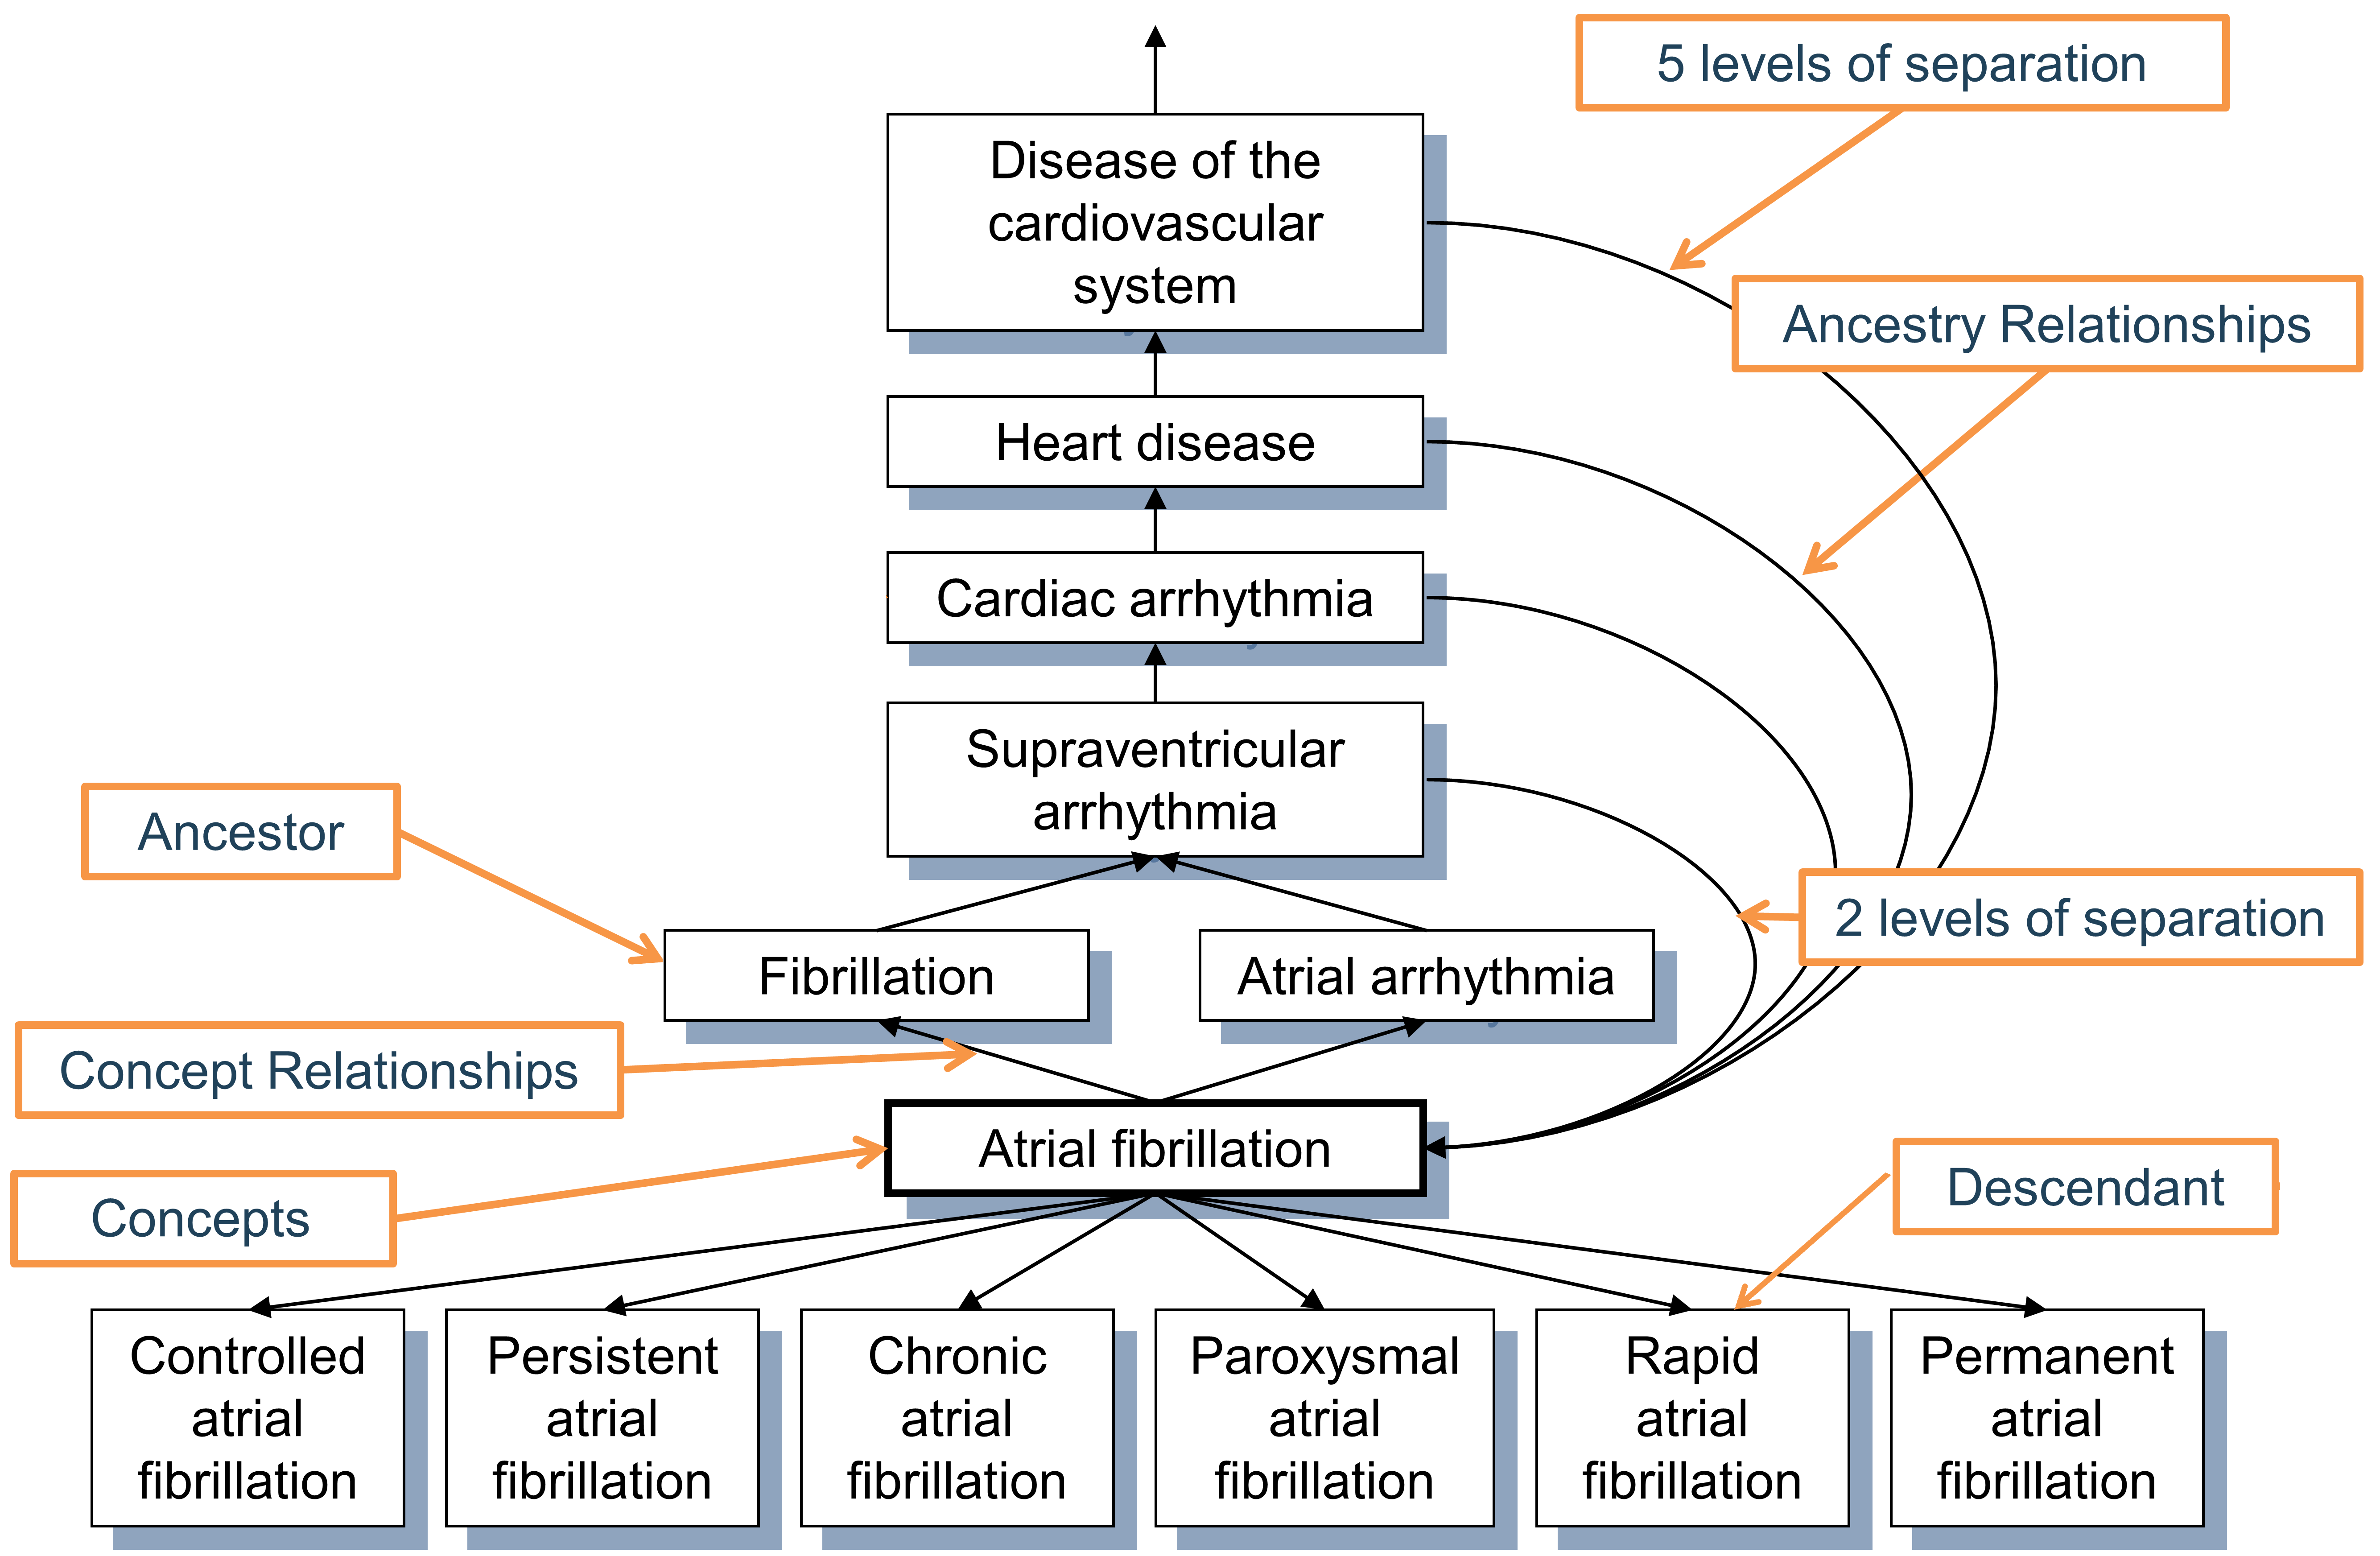
\includegraphics[width=1\linewidth]{images/StandardizedVocabularies/conceptAncestor} 

}

\caption{``심방세동 atrial fibrillation'' condition의 계층. First
degree ancestry는 ``Is a''와 ``Subsumes'' 관계를 통해 정의되며, 모든
higher degree 관계는 추론되고, CONCEPT\_ANCESTOR 표에 저장된다. 각
concept은 분리 수준이 0인 자기 자신의 하위concept이다.
\index{concept!ancestor}}\label{fig:conceptAncestor}
\end{figure}

상위와 하위 항목 사이의 단계(step) 개수를 의미하는 ancestor degree는
MIN\_LEVELS\_OF\_SEPARATION과 MAX\_LEVELS\_OF\_SEPARATION으로 표현되고,
최단 또는 최장의 가능한 연결 정도를 정의해준다. 모든 계층적 관계가 분리
수준 계산에 동일하게 기여하는 것은 아니다. Degree를 구하기 위한 단계는
각 relationship ID에 대한 RELATIONSHIP 참조 테이블의 IS\_HIERARCHICAL
표시 flag로 결정된다.

현재, 고품질의 포괄적인 계층구조는 drug와 condition 두 개의 도메인에만
존재한다. Procedure, measurement, observation 도메인은 부분적으로만
적용되며 현재 구축 중에 있다. 조상(ancestry) concept은 출처, 상품명 또는
다른 속성들과 무관하게 특정 성분이나 약물 등급의 구성원을 가지는 모든
약물을 탐색할 수 있기 때문에 특히 약물 도메인에서 유용하다.

\section{내부 참조 테이블}\label{--}

DOMAIN\_ID, VOCABULARY\_ID, CONCEPT\_CLASS\_ID (셋 모두 CONCEPT
레코드안에 있는) 및 CONCEPT\_RELATIONSHIP\_ID (CONCEPT\_RELATIONSHIP
안에 있는)는 모두 자체 용어집에 의해 제어된다. 이들은 4개의 참조
테이블인 DOMAIN, VOCABULARY, CONCEPT\_CLASS 및 RELATIONSHIP에 정의되어
있으며, *\_ID 필드를 primary keys로 하여 더욱 자세한 *\_NAME 필드 및
*\_CONCEPT\_ID 필드를 포함하는 CONCEPT 테이블에 대한 참조가 포함된 4개의
참조 테이블에 정의되어 있다. 이들 중복 레코드들의 목적은 정보 모델이
자동 탐색 엔진을 허용하도록 지원하기 위한 것이다.

VOCABULARY 테이블에는 기존 vocabulary의 source와 버전을 참조하는
VOCABULARY\_REFERENCE 및 VOCABULARY\_VERSION 필드가 포함되어 있다.
RELATIONSHIP 테이블에는 추가 필드인 DEFINES\_ANCESTRY, IS\_HIERARCHICAL
및 REVERSE\_RELATIONSHIP 필드가 있다. 후자는 한 쌍의 관계에 대해
반대의(counter) relationship ID를 정의한다.

\section{특수 상황}\label{specialSituations}

\subsection{성별}

OMOP CDM 및 표준 용어집의 성별은 출생 시의 생물학적 성별을 나타내지만,
종종 양자택일하는 성별을 어떻게 정의하는지 의문이 제기된다. 이러한
사례들은 OBSERVATION 테이블의 레코드를 통하여 처리해야 하는데, 여기에
개인이 자체적으로 정의한 성별이 저장된다 (데이터 자산에 그런 정보가
포함된 경우).

\subsection{인종과 민족}\label{-}

인종(race)과 민족(ethnicity)은 미국 정부가 지정한 정의를 따른다. 민족은
인종과 상관없이, Hispanic 또는 non-Hispanic 인구에서 분화된 세부
항목으로 구분한다. 인종은 공통적인 상위 5개 인종으로 나뉘며, 계층적
후손으로서 민족성을 가지고 있다. 혼혈 인종은 포함되지 않는다.

\subsection{진단 코딩 체계 및 OMOP
Conditions}\label{----omop-conditions}

ICD-9 또는 ICD-10과 같은 일반적으로 사용되는 코딩 체계는 적절한 진단
작업에 기반하여, 다소 잘 정의된 진단을 명시한다. condition 도메인은
의미론적 공간과 동일하지 않지만, 부분적으로 겹치는 부분이 있다. 예를
들어, conditions에는 진단이 도출되기 전에 기록된 징후와 증상도
포함되어있으며, ICD 코드에는 다른 도메인에 속하는 concept (예를 들어,
procedures) 이 포함되어 있다.

\subsection{시술 코드 시스템}\label{--}

마찬가지로, HCPCS 및 CTP4와 같은 코딩 체계는 의료 시술의 목록으로
간주한다. 실제로, 이 체계들은 의료비 지급 타당성을 선택하는 메뉴에
가깝다. 이러한 서비스의 많은 부분이 procedure 도메인 하에 포함되어
있지만, 많은 concept이 이 도메인 밖에 벗어나 있다.

\subsection{기기}

기기 concept(Device concepts)은 원천 표준 concept에 사용될 수 있는
표준화된 코드 체계를 가지고 있지 않다. 많은 source 데이터에서 기기들은
코드화되어 있지 않고, 외부 코딩 체계에도 포함되지 않는다. 이와 같은
이유로, 현재 사용 가능한 계층 시스템이 없다.

\subsection{방문 및 서비스}\label{--}

방문 concept은 의료 서비스의 성격을 정의한다. 많은 source system에서
병원과 같은 일부 기관이나, 물리적 구조를 나타내는 장소를 서비스
공간이라고 한다. 다른 곳에서는 서비스라고 한다. 방문 concept은 또한
국가마다 다르며, 정의하기 쉽지 않다. 진료 장소(Care sites)는 일반적으로
방문을 몇 번 했는지로 특정한다 (예를 들어, XYZ병원) 그러나 그 방문
숫자만으로는 정의하지는 않아야 한다. (예를 들어, XYZ병원에서 조차
환자들은 진료 목적이 아닌 방문을 할 수도 있기 때문이다)

\subsection{제공자 및 전문의}\label{--}

모든 인간 제공자들은 provider 도메인에 정의되어 있다. 이 제공자들은 의사
및 간호사와 같은 의료 전문가일 수도 있지만, 검안사나, 신발 제조업자와
같은 비의료 서비스 제공자(non-medical provider)일 수도 있다. 전문의는
제공자인 ``의사''(Physician)의 하위concept이다. Care sites는 전문성을
보유할 수 없으나, 주요 직원의 전문성에 의해 정의되는 경우가 많다 (``외과
Surgical department'').

\subsection{특별한 요구사항이 있는 치료 영역}\label{----}

표준 용어들은 포괄적인 방식으로 의료의 모든 측면을 다루고 있다. 하지만,
일부 치료영역에서는 특별한 요구를 가지고 있으며, 특별한 용어집이
필요하다. 예로, 종양학, 방사선학, 유전체학 같은 것이다. Special OHDSI
Working Groups은 이러한 확장 기능을 개발한다. 결과적으로, OMOP 표준
용어집은 통합 시스템을 구성하여 서로 다른 기원과 목적으로 생긴
concept들이 모두 동일한 도메인 특화 계층 내에 존재하게 된다.

\subsection{약물 도메인 내의 표준 concept}\label{rxNormExtension}

Drug 도메인의 많은 concept은 미국 국립 의학 도서관(National Library of
Medicine)이 제공하는 용어집인 RxNorm에서 제공하고 있다. 하지만, 미국 외
지역의 의약품은 미국에서 시판되는 성분, 형태, 강도의 조합 인지에 따라
다뤄지거나 다뤄지지 않을 수도 있다. 미국 시장에 없는 약물은 OHDSI
용어팀에 의해
\href{https://www.ohdsi.org/web/wiki/doku.php?id=documentation:vocabulary:rxnorm_extension}{RxNorm
확장판, RxNorm Extension}이라는 용어집으로 추가되며, 이것은 OHDSI에 의해
유일하게 생성된 큰 도메인 용어집이다.

\subsection{NULL의 특색}\label{null-}

많은 용어집에는 정보가 없는 코드들을 포함하고 있다. 예를 들어, 5개의
성별 concept인 8507 ``Male'', 8532 ``Female'', 8570 ``Ambiguous'', 8551
``Unknown'', 8521 ``기타'' 중 앞의 2개인 8507 ``Male'', 8532
``Female''만 표준이며, 나머지 3개는 매핑이 되어있지 않은 source
concepts이다. 표준 용어집에서는 왜 정보가 없는지에 대한 구분은 없다.
환자가 정보를 철회하거나, 결측값, 정의되지 않거나 표준화되지 않은 값
때문일 수도 있으며 COCEPT\_RELATIONSHIP에 매핑 레코드가 없는 경우 일
수도 있다. 이러한 concept은 매핑되지 않으며, 이는 concept ID = 0인 표준
concept 기본 매핑에 해당한다.

\section{요약}\label{-3}

\BeginKnitrBlock{rmdsummary}
\begin{itemize}
\tightlist
\item
  모든 이벤트 및 관리되는 사건은 OMOP 표준 용어집에 concept, concept
  관계 및 concept 상위 계층으로 표현된다.
\item
  이 중 대부분은 기존의 코딩 체계나 용어집에서 채택해지만, 일부는 OHDSI
  용어팀에서 새로 선별했다.
\item
  모든 concept은 한 개의 도메인을 가지는데, 그런데 그 도메인은
  concept으로 표현되는 그 사건이 CDM의 어떤 테이블에 저장될 지를
  결정한다.
\item
  다른 용어집에서 동등한 의미가 있는 concept들은 그중 하나에 매칭되는데,
  그것이 표준concept으로 지정된 concept이다. 다른 concept들은 원천
  concept들이다.
\item
  매핑은 ``Maps to''와 ``Maps to value'' concept relationships을 통해
  수행된다.
\item
  분류 concept이라 불리는 추가 concept 계층이 있는데, 이는 비표준이지만,
  원천 concept과 달리 계층으로 존재한다. 비표준인, 분류 concept이라고
  불리는 추가적인 concepts class가 있다. 하지만, source concepts과는
  다르게 계층으로 존재한다.
\item
  concept은 시간이 지남에 따라 수명 주기(life-cycle)를 갖는다.
\item
  도메인 내의 concept은 계층으로 구성된다. 계층구조의 품질은 도메인마다
  상이하며, 계층 구조 시스템의 완성을 위해 아직 진행 중이다.
\item
  실수나, 오류를 발견한 경우 커뮤니티에 참여할 것을 적극적으로 권장한다.
\end{itemize}
\EndKnitrBlock{rmdsummary}

\section{예제}\label{-1}

\subsubsection*{전제조건}
\addcontentsline{toc}{subsubsection}{전제조건}

첫 연습에서는, ATHENA\footnote{\url{http://athena.ohdsi.org/}} 또는
ATLAS\footnote{\url{http://atlas-demo.ohdsi.org}}를 이용해서 표준용어집
내에서 concept을 찾아 볼 필요가 있다.

\BeginKnitrBlock{exercise}
\protect\hypertarget{exr:exerciseVocab1}{}{\label{exr:exerciseVocab1}
}``위장관 출혈 gastrointestinal hemorrhage''에 대한 Standard Concept
ID는 무엇인가?
\EndKnitrBlock{exercise}

\BeginKnitrBlock{exercise}
\protect\hypertarget{exr:exerciseVocab2}{}{\label{exr:exerciseVocab2}
}``위장관 출혈 gastrointestinal hemorrhage''에 대한 Standard Concept에
어떤 ICD-10CM 코드가 매핑되는가? 이 Standard Concept에 어떤 ICD-9CM
코드가 매핑되는가?
\EndKnitrBlock{exercise}

\BeginKnitrBlock{exercise}
\protect\hypertarget{exr:exerciseVocab3}{}{\label{exr:exerciseVocab3}
}``위장관 출혈 gastrointestinal hemorrhage''에 대한 Standard concept에
해당하는 MedDRA 선호 용어는 무엇인가?
\EndKnitrBlock{exercise}

제시된 답변은 부록 \ref{Vocabanswers}에서 찾을 수 있다.

\chapter{추출 변환 적재(Extract Transform
Load)}\label{ExtractTransformLoad}

\emph{Chapter leads: Clair Blacketer \& Erica Voss}

\section{서론}

원천 데이터에서 OMOP 공통 데이터 모델(Common Data Model, CDM)을 얻기
위해서는 추출 변환 적재(Extract Transform Load, ETL) 절차가 필요하다. 이
절차는 데이터를 CDM으로 변환하는 과정이며, 표준용어로의 매핑, SQL
코드들을 이용한 자동화된 절차로 이루어지게 된다. ETL 절차는 원천
데이터가 갱신될 때마다 언제든지 재수행할 수 있게끔 반복할 수 있게
구축하는 것이 중요하다.
\index{ETL|see {extract, transform and load (ETL)}} \index{raw data}
\index{native data|see {raw data}} \index{source data|see{raw data}}

ETL을 진행한다는 것은 많은 일을 필요로 한다. 몇 년 동안의 과정을 통해
우리는 4가지 주요 단계로 이루어진 모범사례를 개발하였다.

\begin{enumerate}
\def\labelenumi{\arabic{enumi}.}
\tightlist
\item
  데이터 전문가와 CDM 전문가가 함께 ETL을 설계할 것.
\item
  의학 지식이 있는 사람들이 코드 매핑을 할 것.
\item
  기술자가 ETL을 수행할 것.
\item
  모든 사람이 질 관리에 참여할 것.
\end{enumerate}

이 장에서 우리는 각 단계를 세부적으로 살펴볼 것이다. 각 절차를 보조하기
위해 OHDSI 커뮤니티는 다양한 도구를 개발해 왔고, 이 도구들에 대해서도
다룰 것이다. 마지막으로 CDM과 ETL의 유지에 관해 이야기하며 마무리할
것이다.

\section{1단계 : ETL 설계}\label{-etl-}

ETL 설계와 ETL 수행을 명확하게 분리하는 것이 중요하다. ETL을 설계하는
것은 원천 데이터와 CDM 모두에 대한 넓은 지식이 필요하다. 반대로 ETL을
수행할 때는 ETL을 기술적인 측면에서 효율적으로 수행하는 방법에 대해 기술
전문가들에게 의존하게 된다. 만약 동시에 두 가지 모두를 진행하려 한다면,
전체적인 그림에 집중할 때보다 세부적인 사항에서 막히게 될 가능성이 높다.

ETL 설계를 위해 두 가지 밀접하게 연관된 도구들을 개발하였다: White
Rabbit과 Rabbit-in-a-Hat

\subsection{White Rabbit}\label{white-rabbit}

ETL 절차를 시작하기 위해서는 테이블, 필드, 내용을 포함한 데이터에 대한
이해가 필요하다. 하단의 링크에
\href{https://github.com/OHDSI/WhiteRabbit}{White Rabbit}에 대한 정보가
기록되어 있다. White Rabbit은 보건의료 종단(longitudinal)
데이터베이스에서 \href{https://github.com/OHDSI/CommonDataModel}{OMOP
CDM}으로의 ETL 작업 준비를 도와주기 위한 소프트웨어이다. White Rabbit은
원천 데이터를 탐색하고 ETL 설계를 시작하기 위한 필수 정보에 대한
보고서를 생성해준다. 모든 소스 코드, 설치 방법 및 설명서는
깃헙(Github)에서 확인할 수 있다.\footnote{\url{https://github.com/OHDSI/WhiteRabbit}.}
\index{White Rabbit} \index{data profiling|see {White Rabbit}}

\subsubsection*{범위와 목표}\label{-}
\addcontentsline{toc}{subsubsection}{범위와 목표}

White Rabbit의 주요 기능은 원천 데이터에 대한 탐색을 수행하고, 테이블,
필드, 필드 값들에 대한 세부적인 정보를 제공하는 것이다. 원천 데이터는
comma-seperated(CSV) 텍스트 파일일 수도 있고, 데이터베이스(MySQL, SQL
Server, Oracle, PostgreSQL, Microsoft APS, Microsoft Access, Amazon
RedShift)에 적재되어 있을 수도 있다. 탐색 과정에서 Rabbit-In-a-Hat
도구와 함께 쓴다면 ETL을 설계할 때 참고할 수 있는 보고서를 생성할 수
있다. White Rabbit은 다른 표준 데이터 프로파일링 도구들과는 달리 개인
식별 정보(Personally Identifiable Information, PII)가 결과 데이터
파일에서 보이는 것을 방지한다.

\subsubsection*{절차 개요}\label{-}
\addcontentsline{toc}{subsubsection}{절차 개요}

원천 데이터를 탐색하기 위해 소프트웨어를 사용하는 일반적인 순서:

\begin{enumerate}
\def\labelenumi{\arabic{enumi}.}
\tightlist
\item
  결과를 내보낼 작업 폴더를 로컬 컴퓨터에 설정.
\item
  데이터베이스 혹은 CSV 텍스트 파일과의 연결 및 연결 확인.
\item
  탐색 대상 테이블 선택 및 탐색.
\item
  White Rabbit의 원천 데이터에 대한 정보 생성 및 내보내기.
\end{enumerate}

\subsubsection*{작업 폴더 설정}\label{--}
\addcontentsline{toc}{subsubsection}{작업 폴더 설정}

White Rabbit 어플리케이션의 다운로드 및 설치 이후, 처음으로 할 일은 작업
폴더를 설정하는 것이다. White Rabbit이 생성하는 모든 파일은 설정한 로컬
폴더에 생성될 것이다. 그림 \ref{fig:WhiteRabbitLocation}에서 보이는
``Pick Folder'' 버튼을 사용하여 탐색 문서들이 저장될 로컬 환경을 탐색할
수 있다.

\begin{figure}

{\centering 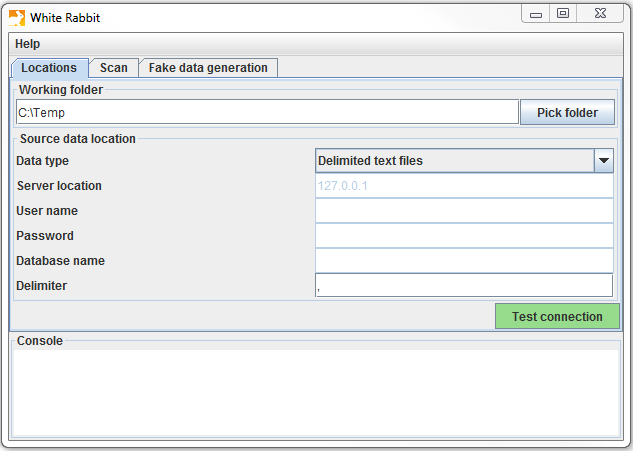
\includegraphics[width=1\linewidth]{images/ExtractTransformLoad/WhiteRabbitLocation} 

}

\caption{"Pick Folder" 버튼은 White Rabbit 어플리케이션의 작업 폴더 사양을 허용한다.}\label{fig:WhiteRabbitLocation}
\end{figure}

\subsubsection*{데이터베이스 연결}\label{-}
\addcontentsline{toc}{subsubsection}{데이터베이스 연결}

White Rabbit은 구분자로 구분된 텍스트 파일(CSV)과 다양한 데이터베이스
플랫폼들을 지원한다. 다양한 필드들에 대한 필요 항목들의 설명을 보려면
마우스를 올려야 한다. 더욱 자세한 설명은 설명서에서 확인할 수 있다.

\subsubsection*{데이터베이스 테이블 탐색}\label{--}
\addcontentsline{toc}{subsubsection}{데이터베이스 테이블 탐색}

데이터베이스에 연결한 이후에는 데이터베이스에 적재되어있는 테이블을
탐색할 수 있다. 탐색 과정은 ETL을 설계하는 데 도움이 되는 원천 데이터에
대한 정보를 담은 보고서를 생성할 수 있다. 그림
\ref{fig:WhiteRabbitAddTables}에 보이는 Scan 탭의 ``Add'' (Ctrl + mouse
click) 버튼을 눌러서 선택된 원천 데이터베이스의 각 테이블을 선택하거나,
``Add all in DB'' 누름으로써 모든 테이블을 자동으로 선택할 수 있다.

\begin{figure}

{\centering 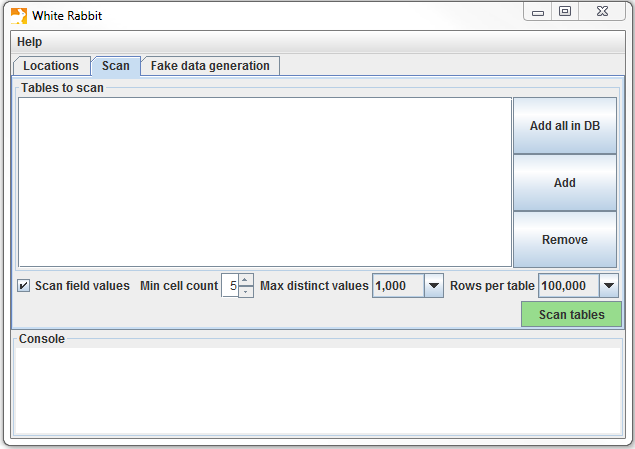
\includegraphics[width=1\linewidth]{images/ExtractTransformLoad/WhiteRabbitAddTables} 

}

\caption{White Rabbit Scan 탭.}\label{fig:WhiteRabbitAddTables}
\end{figure}

탐색에 사용될 몇 가지 옵션들:

\begin{itemize}
\tightlist
\item
  ``Scan field values'' 는 열에 어떠한 값들이 나타나는지 보고 싶을 때
  사용한다.
\item
  ``Min cell count'' 는 필드 값을 탐색할 때 쓰이는 옵션이다. 기본값은
  5로 설정되어 있으며, 이는 원천 데이터에서 5번 이하로 나타나는 값은
  보고서에 나타내지 않는 것을 의미한다. 각 데이터 세트들은 각각의 고유한
  규칙에 따라 minimal cell count를 정해야 할 것이다.
\item
  ``Rows per table'' 는 필드값을 탐색할 때 쓰이는 옵션이다. 기본값으로
  White Rabbit은 테이블에서 무작위로 100,000개의 행을 선택하여 탐색할
  것이다.
\end{itemize}

모든 옵션이 설정된 이후에는 ``Scan tables''을 누르면 된다. 탐색이 완료된
이후에는 보고서가 작업 폴더에 생성될 것이다.

\subsubsection*{탐색 보고서의 이해}\label{--}
\addcontentsline{toc}{subsubsection}{탐색 보고서의 이해}

탐색이 완료된 이후에는 선택된 작업 폴더에 엑셀 파일이 생성될 것이며,
엑셀 파일에는 스캔한 각 테이블에 대한 하나의 탭과 개요 탭이 생성된다.
개요 탭은 탐색한 모든 테이블이며, 각 테이블의 필드, 각 필드의 데이터
타입, 필드의 최대 길이, 테이블의 행의 수, 탐색한 행의 수, 그리고 얼마나
많은 필드가 비어있는지 보여준다. 그림 \ref{fig:ScanOverviewTab}은 개요
탭의 예시를 보여준다.

\begin{figure}

{\centering 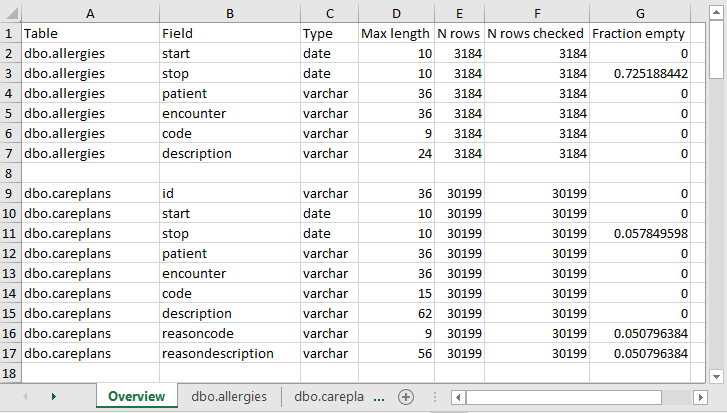
\includegraphics[width=1\linewidth]{images/ExtractTransformLoad/ScanOverviewTab} 

}

\caption{검색 리포트의 개요 탭 예시.}\label{fig:ScanOverviewTab}
\end{figure}

각 테이블의 탭들은 각각의 필드, 필드의 값들, 그리고 값들의 빈도를
나타낸다. 각 원천 테이블의 칼럼들은 엑셀에서 두 개의 칼럼으로 생성된다.
하나는 탐색 시 설정한 ``Min cell count'' 보다 큰 값들의 고유한 값을
보여준다. 만약 고유한 값 목록이 잘려있다면, 목록의 마지막 값은 ``List
truncated'' 가 될 것이다; 이는 하나 혹은 그 이상의 값들이 ``Min cell
count'' 보다 작은 고유한 값이 있음을 나타낸다. 각각의 고유한 값 옆에는
빈도를 나타내는 두 번째 칼럼이 있다 (표본에서 값이 발생하는 횟수). 이 두
칼럼 (고유한 값과 빈도수) 은 작업 책(workbook)의 프로파일링 된 테이블의
모든 원천 변수들에 대해 반복돼서 나타난다.

\begin{figure}

{\centering 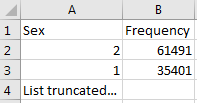
\includegraphics[width=0.3\linewidth]{images/ExtractTransformLoad/ScanSex} 

}

\caption{단일 열에 대한 예제 값.}\label{fig:scanSex}
\end{figure}

보고서는 원천 데이터에 무엇이 있는지를 강조함으로써 데이터를 이해하는 데
강력한 도움을 준다. 예를 들면, 그림 \ref{fig:scanSex}에 나타난 결과가
탐색된 테이블 칼럼 중 하나인 ``Sex''에 반환될 경우, 우리는 각각
61,491번과 35,401번 나타난 공통된 값들(1과 2)이 있음을 알 수 있다. White
Rabbit은 1을 남성으로, 2를 여성으로 정의하지는 않을 것이다; 데이터
소유자가 일반적으로 원천 시스템에 고유한 원천 코드를 정의해야 한다.
하지만 이 두 가지 값(1 \& 2)들은 데이터에 있는 유일한 값들이 아니기
때문에 우리는 잘린 목록을 확인해야 한다. 이 값들은 (``Min cell count''
정의에 따라) 매우 낮은 빈도로 나타나게 되고, 종종 부정확하거나 매우
의심스러운 값들로 표현된다. ETL 수행을 계획할 때 우리는 높은 빈도의 성별
개념으로써 1과 2만 다루는 것이 아니라, 칼럼에 존재하는 낮은 빈도의
값들도 고려해야 한다. 예를 들어 만약 낮은 빈도의 성별들이 ``NULL''일
경우 ETL 진행 시 이러한 데이터에 대해 어떻게 처리할 것인지 확실히 해야
한다.

\subsection{Rabbit-In-a-Hat}\label{rabbit-in-a-hat}

White Rabbit과 함께 우리는 원천 데이터에 대한 분명한 그림을 그릴 수
있다. 또한, 우리는 CDM에 대한 전체 명세서를 알고 있다. 이제 우리는
하나에서 다른 하나로 넘어갈 로직을 정의해야 한다. 이 설계 활동은 원천
데이터와 CDM 모두에 대한 온전한 지식을 요구한다. White Rabbit
소프트웨어와 함께 사용되는 Rabbit-in-a-Hat 도구는 명확하게 이 분야의
전문가들을 위해 개발되었다. 일반적으로 ETL 설계팀은 회의실에 같이 앉아
Rabbit-in-a-Hat을 프로젝터 화면으로 같이 보면서 작업을 한다. 첫 번째로
테이블 간의 매핑은 협력적으로 결정될 수 있으며, 그 후에는 필드 간의
매핑이 설계되는 동시에 어떠한 값들을 변환시킬지 로직을 정의할 수 있다.
\index{Rabbit-In-A-Hat} \index{ETL design|see {Rabbit-In-A-Hat}}

\subsubsection*{범위와 목표}\label{--1}
\addcontentsline{toc}{subsubsection}{범위와 목표}

Rabbit-In-a-Hat은 White Rabbit의 탐색 문서를 읽고 시각화하기 위해
설계되었다. White Rabbit은 원천 데이터에 대한 정보를 생성하는 반면,
Rabbit-In-a-Hat은 그 정보를 사용하고 그래픽 사용자 인터페이스를 통하여
사용자들이 원천 데이터의 테이블과 칼럼들을 CDM으로 연결될 수 있게
해준다. Rabbit-In-a-Hat은 ETL 절차에 대한 문서를 생성해주지만 ETL을 위한
코드는 생성하지 않는다.

\subsubsection*{절차 개요}\label{--1}
\addcontentsline{toc}{subsubsection}{절차 개요}

소프트웨어를 이용한 ETL 문서 생성을 위한 일반적인 순서:

\begin{enumerate}
\def\labelenumi{\arabic{enumi}.}
\tightlist
\item
  White Rabbit이 완료한 탐색 결과.
\item
  탐색 결과 열기; 인터페이스가 원천 테이블들과 CDM 테이블들을 보여줌.
\item
  원천 테이블의 정보와 상응하는 CDM 테이블을 연결.
\item
  CDM 테이블에 상응하는 각 원천 테이블들에 대해서 세부적인 원천 칼럼과
  CDM 칼럼의 연결을 정의.
\item
  Rabbit-In-a-Hat 작업을 저장하고 MS 워드 문서로 내보내기.
\end{enumerate}

\subsubsection*{ETL 로직 작성}\label{etl--}
\addcontentsline{toc}{subsubsection}{ETL 로직 작성}

일단 Rabbit-In-a-Hat 내의 White Rabbit 탐색 보고서를 확인한다면, 원천
데이터를 OMOP CDM으로 변환하는 설계와 로직 작성을 시작할 준비가 되었다.
하나의 예시로써 하단의 장들에서 Synthea\footnote{Synthea\textsuperscript{TM}
  is a patient generator that aims to model real patients. Data are
  created based on parameters passed to the application.The structure of
  the data can be found here:
  \url{https://github.com/synthetichealth/synthea/wiki}.} 데이터베이스의
일부 테이블들의 변환을 보여줄 것이다.

\subsubsection*{ETL의 일반적인 흐름}\label{etl--}
\addcontentsline{toc}{subsubsection}{ETL의 일반적인 흐름}

CDM이 사람 중심의 모형이기 때문에 제일 먼저 PERSON 테이블 매핑으로
시작하는 것이 좋다. 모든 임상 사건과 관련 있는 테이블들
(CONDITION\_OCCURRENCE, DRUG\_EXPOSURE, PROCEDURE\_OCCURRENCE 기타 등)
은 PERSON 테이블의 person\_id를 참조하기에 PERSON 테이블에 대한 로직을
먼저 작성하는 것이 나중을 위해 좋다. PERSON 테이블을 변환한 다음에는
OBSERVATION\_PERIOD를 변환하는 것이 좋은 선택이다. CDM 데이터베이스의
개인은 최소 하나 이상의 OBSERVATION\_PERIOD를 가져야 하고, 일반적으로 한
사람에 대한 모든 사건은 이 관찰 기간 내에 들어온다. PERSON과
OBSERVATION\_PERIOD 테이블이 완료되면 보통 PROVIDER, CARE\_SITE, 그리고
LOCATION과 같은 테이블이 다음 대상이 된다. 임상 테이블 이전에 마지막으로
로직을 작성해야 하는 테이블은 VISIT\_OCCURRENCE이다. 한 사람이
환자로서의 여정에서 대부분의 사건이 방문할 때 발생하기 때문에 종종 모든
ETL 과정에서 가장 복잡하고 중요한 부분이기도 하다. 일단, 이 테이블들이
완료되면 어떤 CDM 테이블들 어떤 순서대로 매핑할지는 선택하기 나름이다.

\begin{figure}

{\centering 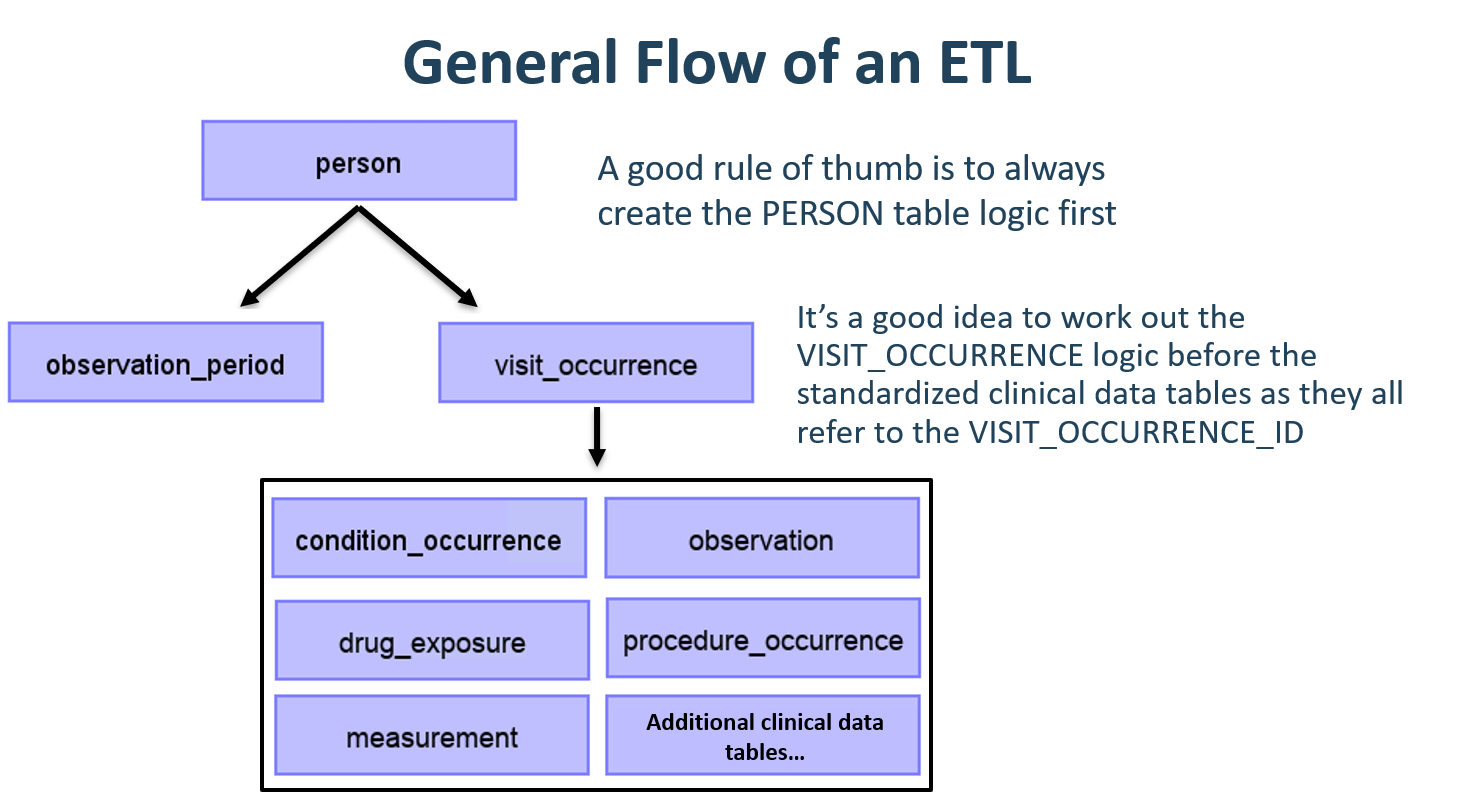
\includegraphics[width=1\linewidth]{images/ExtractTransformLoad/flowOfEtl} 

}

\caption{ETL의 일반적인 흐름과 먼저 매핑할 테이블.}\label{fig:etlFlow}
\end{figure}

CDM 변환 과정에서 종종 중간 테이블들을 만들 필요가 있을 수 있다. 올바른
VISIT\_OCCURRENCE\_ID를 해당 사건에 부여하거나 아니면 원천 코드를 표준
코드로 매핑하는 경우일 수도 있다 (이 단계는 종종 매우 느리게 진행된다).
중간 테이블은 100\% 허용되고 장려된다. 하지만 이러한 중간 테이블이
변환이 완료된 이후에도 남아있거나 사용하는 것은 추천하지 않는다.

\subsubsection*{매핑 예시: PERSON 테이블}\label{--person-}
\addcontentsline{toc}{subsubsection}{매핑 예시: PERSON 테이블}

Synthea 데이터 구조에서 환자 테이블은 20개의 열을 갖고 있지만 그림
\ref{fig:syntheaPerson}에서 보이는 것처럼 모든 열이 PERSON 테이블에
필요한 것은 아니다. 이런 일은 매우 흔한 일이고 문제가 되지 않는다. 이
예시에서는 환자 이름, 운전면허번호, 여권 번호 등 Synthea의 환자 테이블의
많은 데이터 포인트가 CDM PERSON 테이블에 사용되지 않는 것을 알 수 있다.

\begin{figure}

{\centering 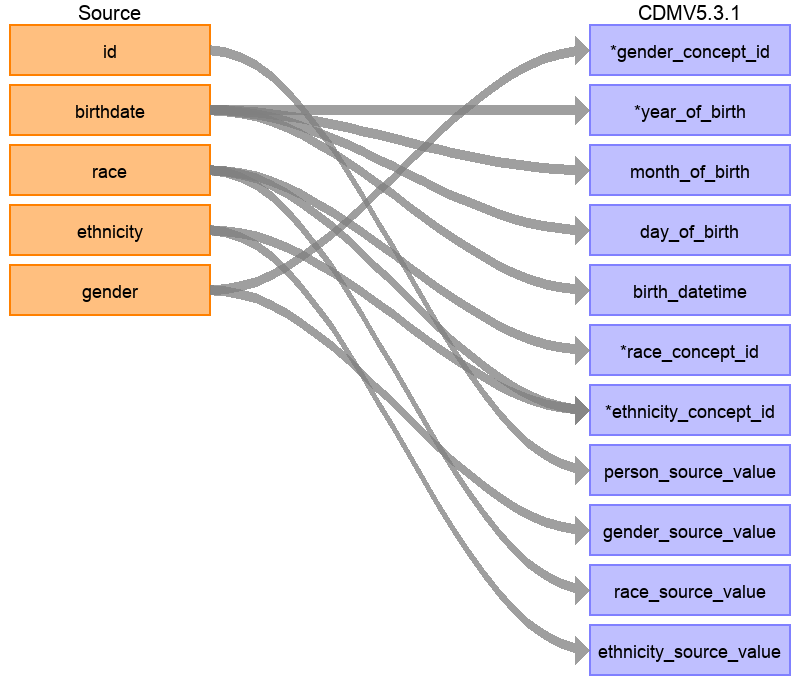
\includegraphics[width=1\linewidth]{images/ExtractTransformLoad/syntheaPersonTable} 

}

\caption{CDM PERSON 테이블에 Synta Patients 테이블 매핑.}\label{fig:syntheaPerson}
\end{figure}

하단의 표 \ref{tab:syntheaEtlPerson}은 Synthea의 환자 테이블이 CDM
PERSON 테이블로 변환되는 로직을 보여준다. `Destination Field'는 CDM
데이터의 어디에 매핑되는지를 나타낸다. `Source field'는 원천 테이블
(예시에서는 환자 테이블) 의 어느 열에서 CDM의 열로 변하는지 나타낸다.
마지막으로, `Logic \& comments'는 로직에 대한 설명을 의미한다.

\begin{longtable}[]{@{}lll@{}}
\caption{\label{tab:syntheaEtlPerson} Synthea 환자 테이블을 CDM PERSON
테이블에 변환하기 위한 ETL 로직}\tabularnewline
\toprule
\begin{minipage}[b]{0.28\columnwidth}\raggedright\strut
Destination Field\strut
\end{minipage} & \begin{minipage}[b]{0.13\columnwidth}\raggedright\strut
Source field\strut
\end{minipage} & \begin{minipage}[b]{0.50\columnwidth}\raggedright\strut
Logic \& comments\strut
\end{minipage}\tabularnewline
\midrule
\endfirsthead
\toprule
\begin{minipage}[b]{0.28\columnwidth}\raggedright\strut
Destination Field\strut
\end{minipage} & \begin{minipage}[b]{0.13\columnwidth}\raggedright\strut
Source field\strut
\end{minipage} & \begin{minipage}[b]{0.50\columnwidth}\raggedright\strut
Logic \& comments\strut
\end{minipage}\tabularnewline
\midrule
\endhead
\begin{minipage}[t]{0.28\columnwidth}\raggedright\strut
PERSON\_ID\strut
\end{minipage} & \begin{minipage}[t]{0.13\columnwidth}\raggedright\strut
\strut
\end{minipage} & \begin{minipage}[t]{0.50\columnwidth}\raggedright\strut
Autogenerate. The PERSON\_ID will be generated at the time of
implementation. This is because the id value from the source is a
varchar value while the PERSON\_ID is an integer. The id field from the
source is set as the PERSON\_SOURCE\_VALUE to preserve that value and
allow for error-checking if necessary.\strut
\end{minipage}\tabularnewline
\begin{minipage}[t]{0.28\columnwidth}\raggedright\strut
GENDER\_CONCEPT\_ID\strut
\end{minipage} & \begin{minipage}[t]{0.13\columnwidth}\raggedright\strut
gender\strut
\end{minipage} & \begin{minipage}[t]{0.50\columnwidth}\raggedright\strut
When gender = `M' then set GENDER\_CONCEPT\_ID to 8507, when gender =
`F' then set to 8532. Drop any rows with missing/unknown gender. These
two concepts were chosen as they are the only two standard concepts in
the gender domain. The choice to drop patients with unknown genders
tends to be site-based, though it is recommended they are removed as
people without a gender are excluded from analyses.\strut
\end{minipage}\tabularnewline
\begin{minipage}[t]{0.28\columnwidth}\raggedright\strut
YEAR\_OF\_BIRTH\strut
\end{minipage} & \begin{minipage}[t]{0.13\columnwidth}\raggedright\strut
birthdate\strut
\end{minipage} & \begin{minipage}[t]{0.50\columnwidth}\raggedright\strut
Take year from birthdate\strut
\end{minipage}\tabularnewline
\begin{minipage}[t]{0.28\columnwidth}\raggedright\strut
MONTH\_OF\_BIRTH\strut
\end{minipage} & \begin{minipage}[t]{0.13\columnwidth}\raggedright\strut
birthdate\strut
\end{minipage} & \begin{minipage}[t]{0.50\columnwidth}\raggedright\strut
Take month from birthdate\strut
\end{minipage}\tabularnewline
\begin{minipage}[t]{0.28\columnwidth}\raggedright\strut
DAY\_OF\_BIRTH\strut
\end{minipage} & \begin{minipage}[t]{0.13\columnwidth}\raggedright\strut
birthdate\strut
\end{minipage} & \begin{minipage}[t]{0.50\columnwidth}\raggedright\strut
Take day from birthdate\strut
\end{minipage}\tabularnewline
\begin{minipage}[t]{0.28\columnwidth}\raggedright\strut
BIRTH\_DATETIME\strut
\end{minipage} & \begin{minipage}[t]{0.13\columnwidth}\raggedright\strut
birthdate\strut
\end{minipage} & \begin{minipage}[t]{0.50\columnwidth}\raggedright\strut
With midnight as time 00:00:00. Here, the source did not supply a time
of birth so the choice was made to set it at midnight.\strut
\end{minipage}\tabularnewline
\begin{minipage}[t]{0.28\columnwidth}\raggedright\strut
RACE\_CONCEPT\_ID\strut
\end{minipage} & \begin{minipage}[t]{0.13\columnwidth}\raggedright\strut
race\strut
\end{minipage} & \begin{minipage}[t]{0.50\columnwidth}\raggedright\strut
When race = `WHITE' then set as 8527, when race = `BLACK' then set as
8516, when race = `ASIAN' then set as 8515, otherwise set as 0. These
concepts were chosen because they are the standard concepts belonging to
the race domain that most closely align with the race categories in the
source.\strut
\end{minipage}\tabularnewline
\begin{minipage}[t]{0.28\columnwidth}\raggedright\strut
ETHNICITY\_ CONCEPT\_ID\strut
\end{minipage} & \begin{minipage}[t]{0.13\columnwidth}\raggedright\strut
race ethnicity\strut
\end{minipage} & \begin{minipage}[t]{0.50\columnwidth}\raggedright\strut
When race = `HISPANIC', or when ethnicity in (`CENTRAL\_AMERICAN',
`DOMINICAN', `MEXICAN', `PUERTO\_RICAN', `SOUTH\_AMERICAN') then set as
38003563, otherwise set as 0. This is a good example of how multiple
source columns can contribute to one CDM column. In the CDM ethnicity is
represented as either Hispanic or not Hispanic so values from both the
source column race and source column ethnicity will determine this
value.\strut
\end{minipage}\tabularnewline
\begin{minipage}[t]{0.28\columnwidth}\raggedright\strut
LOCATION\_ID\strut
\end{minipage} & \begin{minipage}[t]{0.13\columnwidth}\raggedright\strut
\strut
\end{minipage} & \begin{minipage}[t]{0.50\columnwidth}\raggedright\strut
\strut
\end{minipage}\tabularnewline
\begin{minipage}[t]{0.28\columnwidth}\raggedright\strut
PROVIDER\_ID\strut
\end{minipage} & \begin{minipage}[t]{0.13\columnwidth}\raggedright\strut
\strut
\end{minipage} & \begin{minipage}[t]{0.50\columnwidth}\raggedright\strut
\strut
\end{minipage}\tabularnewline
\begin{minipage}[t]{0.28\columnwidth}\raggedright\strut
CARE\_SITE\_ID\strut
\end{minipage} & \begin{minipage}[t]{0.13\columnwidth}\raggedright\strut
\strut
\end{minipage} & \begin{minipage}[t]{0.50\columnwidth}\raggedright\strut
\strut
\end{minipage}\tabularnewline
\begin{minipage}[t]{0.28\columnwidth}\raggedright\strut
PERSON\_SOURCE\_ VALUE\strut
\end{minipage} & \begin{minipage}[t]{0.13\columnwidth}\raggedright\strut
id\strut
\end{minipage} & \begin{minipage}[t]{0.50\columnwidth}\raggedright\strut
\strut
\end{minipage}\tabularnewline
\begin{minipage}[t]{0.28\columnwidth}\raggedright\strut
GENDER\_SOURCE\_ VALUE\strut
\end{minipage} & \begin{minipage}[t]{0.13\columnwidth}\raggedright\strut
gender\strut
\end{minipage} & \begin{minipage}[t]{0.50\columnwidth}\raggedright\strut
\strut
\end{minipage}\tabularnewline
\begin{minipage}[t]{0.28\columnwidth}\raggedright\strut
GENDER\_SOURCE\_ CONCEPT\_ID\strut
\end{minipage} & \begin{minipage}[t]{0.13\columnwidth}\raggedright\strut
\strut
\end{minipage} & \begin{minipage}[t]{0.50\columnwidth}\raggedright\strut
\strut
\end{minipage}\tabularnewline
\begin{minipage}[t]{0.28\columnwidth}\raggedright\strut
RACE\_SOURCE\_ VALUE\strut
\end{minipage} & \begin{minipage}[t]{0.13\columnwidth}\raggedright\strut
race\strut
\end{minipage} & \begin{minipage}[t]{0.50\columnwidth}\raggedright\strut
\strut
\end{minipage}\tabularnewline
\begin{minipage}[t]{0.28\columnwidth}\raggedright\strut
RACE\_SOURCE\_ CONCEPT\_ID\strut
\end{minipage} & \begin{minipage}[t]{0.13\columnwidth}\raggedright\strut
\strut
\end{minipage} & \begin{minipage}[t]{0.50\columnwidth}\raggedright\strut
\strut
\end{minipage}\tabularnewline
\begin{minipage}[t]{0.28\columnwidth}\raggedright\strut
ETHNICITY\_ SOURCE\_VALUE\strut
\end{minipage} & \begin{minipage}[t]{0.13\columnwidth}\raggedright\strut
ethnicity\strut
\end{minipage} & \begin{minipage}[t]{0.50\columnwidth}\raggedright\strut
In this case the ETHNICITY\_SOURCE\_VALUE will have more granularity
than the ETHNICITY\_CONCEPT\_ID.\strut
\end{minipage}\tabularnewline
\begin{minipage}[t]{0.28\columnwidth}\raggedright\strut
ETHNICITY\_ SOURCE\_CONCEPT\_ID\strut
\end{minipage} & \begin{minipage}[t]{0.13\columnwidth}\raggedright\strut
\strut
\end{minipage} & \begin{minipage}[t]{0.50\columnwidth}\raggedright\strut
\strut
\end{minipage}\tabularnewline
\bottomrule
\end{longtable}

Synthea 데이터의 CDM으로의 변환에 대한 더 자세한 설명은 전체 명세서를
참고하면 된다.\footnote{\url{https://ohdsi.github.io/ETL-Synthea/}}

\section{2단계: 코드 매핑 생성}\label{---}

점점 더 많은 원천 코드가 OMOP 용어에 추가되고 있다. 이것은 CDM으로
변환된 데이터의 코딩 체계가 이미 CDM에 포함되거나 매핑되었을 수도 있다는
것을 의미한다. OMOP Vocabulary의 VOCABULARY 테이블을 통해 어떤 용어들이
포함되었는지 확인할 수 있다. 비표준인 원천 코드 (예를 들어 ICD-10CM
codes) 에서 표준용어 (예를 들어 SNOMED codes) 로의 매핑을 확인하려면
CONCEPT\_RELATIONSHIP 테이블 내의 relationship\_id = ``Maps to'' 인
값들을 찾으면 확인할 수 있다. 예를 들면 ICD-10CM 코드 `I21' (``Acute
Myocardial Infarction'') 의 표준용어 ID를 확인하기 위해 다음과 같은
SQL을 사용할 수 있다:

\begin{Shaded}
\begin{Highlighting}[]
\KeywordTok{SELECT}\NormalTok{ concept_id_2 standard_concept_id}
\KeywordTok{FROM}\NormalTok{ concept_relationship}
\KeywordTok{INNER} \KeywordTok{JOIN}\NormalTok{ concept source_concept}
  \KeywordTok{ON}\NormalTok{ concept_id = concept_id_}\DecValTok{1}
\KeywordTok{WHERE}\NormalTok{ concept_code = }\StringTok{'I21'}
  \KeywordTok{AND}\NormalTok{ vocabulary_id = }\StringTok{'ICD10CM'}
  \KeywordTok{AND}\NormalTok{ relationship_id = }\StringTok{'Maps to'}\NormalTok{; }
\end{Highlighting}
\end{Shaded}

\begin{longtable}[]{@{}r@{}}
\toprule
STANDARD\_CONCEPT\_ID\tabularnewline
\midrule
\endhead
312327\tabularnewline
\bottomrule
\end{longtable}

하지만 가끔은 원천 데이터가 용어집에 없는 코딩 시스템을 사용할 수도
있다. 이러한 경우에는 원천 코딩 시스템을 표준 개념으로 변환하는 매핑을
정의하여야 한다. 하지만 원천 코딩 시스템에 많은 수의 용어가 있으면 코드
매핑이 어려울 수도 있다. 이를 쉽게 진행하기 위한 몇 가지 참고사항이
있다.

\begin{itemize}
\tightlist
\item
  가장 높은 빈도의 코드에 집중. 절대 쓰이지 않는 코드나 거의 안 쓰이는
  코드는 실제 연구에서도 쓰이지 않기 때문에 많은 노력을 들여서 매핑을
  진행할 필요가 없다.
\item
  가능하면 기존의 정보를 활용. 예를 들어 많은 국가 약물 코딩 시스템은
  이미 ATC로 매핑되어있다. 비록 ATC가 많은 목적에 대해 세부적으로
  부합하지는 않지만, ATC와 RxNorm의 관계를 통해 어떤 RxNorm 코드가
  사용되는지 추측할 수는 있다.
\item
  Usagi를 사용한다.
\end{itemize}

\subsection{Usagi}\label{usagi}

Usagi는 코드 매핑 절차를 도와주는 도구이다. Usagi는 코드 설명의 단어
유사도에 기반하여 매핑을 추천할 수 있다. 만약 원천 코드가 외국어로만
확인 가능하다면, Google Translate\footnote{\url{https://translate.google.com/}}를
통해 종종 해당 용어의 훌륭한 영어 번역을 확인할 수 있다. Usagi의 자동
추천이 정확하지 않을 경우 사용자가 직접 적절한 목표 개념을 찾을 수 있다.
최종적으로 사용자는 어떤 매핑이 ETL에 사용될 수 있는지 지정할 수 있다.
Usagi는 GitHub\footnote{\url{https://github.com/OHDSI/Usagi}}을 통해
사용할 수 있다. \index{Usagi} \index{source code mapping|see {Usagi}}

\subsubsection*{범위와 목표}\label{--2}
\addcontentsline{toc}{subsubsection}{범위와 목표}

매핑이 필요한 원천 코드를 Usagi로 불러올 수 있다 (만약 코드가 영어가
아닐 경우, 추가로 번역한 열이 필요하다). 단어 유사도 접근법은 원천
코드와 Vocabulary 개념들을 연결하기 위해 필요하다. 하지만 이러한 코드
연결은 수동적으로 검토해야 하고, Usagi는 이를 수행하기 위한 인터페이스를
제공한다. Usagi는 Vocabulary에 표준 개념만을 제안한다.

\subsubsection*{절차 개요}\label{--2}
\addcontentsline{toc}{subsubsection}{절차 개요}

소프트웨어를 사용하기 위한 일반적인 순서:

\begin{enumerate}
\def\labelenumi{\arabic{enumi}.}
\tightlist
\item
  원천 시스템 (``원천 코드'') 로부터 Vocabulary concepts들로의 매핑을
  진행하고 싶은 코드들을 올림.
\item
  Usagi 단어 유사도 접근법을 이용하여 Vocabulary concepts들로의 매핑을
  진행.
\item
  Usagi 인터페이스를 활용하여 제안된 매핑을 확인하고 필요할 경우 개선.
  코딩 시스템과 의학 지식이 있는 사람이 리뷰를 진행하는 것이 바람직함.
\item
  매핑 결과를 Vocabulary의 SOURCE\_TO\_CONCEPT\_MAP으로 내보냄.
\end{enumerate}

\subsubsection{Usagi로 원천 코드 가져오기}\label{usagi---}

원천 시스템에서 CSV나 엑셀 (.xlsx) 파일로 원천 코드를 내보낸다. 이때
파일은 원천 코드와 영어 코드 설명에 대한 열들이 있어야 하지만, 추가적인
정보 역시 더할 수 있다 (예를 들어 약물 용량, 번역되었을 경우 원래
언어로의 코드 설명). 게다가 원천 코드에 대한 정보 뿐만 아니라, 어떤
코드를 먼저 매핑해야 할지 정하는 데 도움이 되기 때문에 빈도 역시
포함하는 것이 좋다 (예를 들어 1,000개의 원천 코드를 가져올 수 있지만,
100개만 실제 시스템에 정말로 사용되는 경우). 만약 원천 코드가 영어로의
번역이 필요할 경우, Google Translate가 도움이 될 수 있다.

참고: 원천 코드는 도메인 (다시 말하면 drugs, procedures, conditions,
observations) 별로 분류되어야 하며, 하나의 파일로 묶여서는 안 된다.

파일로부터 원천 코드를 Usagi로 올린다 -\textgreater{} 코드 메뉴를
가져온다. 여기서 ``Import codes \ldots{}''는 그림
\ref{fig:usagiImport}과 같이 보일 것이다. 이 그림에서 원천 코드 용어들은
네덜란드어이고, 영어로 번역되어있다. Usagi는 표준용어로의 매핑을 위해
영어 번역을 이용할 것이다.

\begin{figure}

{\centering 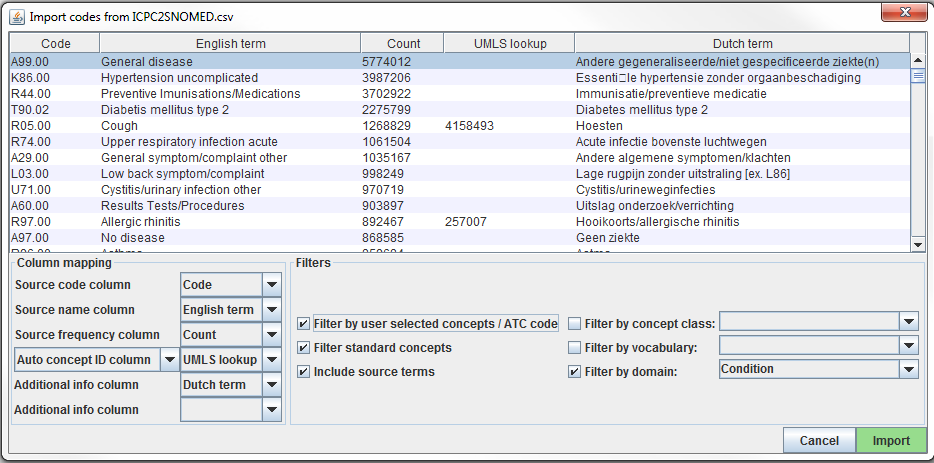
\includegraphics[width=1\linewidth]{images/ExtractTransformLoad/usagiImport} 

}

\caption{Usagi 소스코드 입력화면.}\label{fig:usagiImport}
\end{figure}

``Column mapping'' 부분 (왼쪽 아래) 은 Usagi가 불러온 테이블을 어떻게
사용할 것인지 정하는 단계이다. 마우스를 끌어다 놓으면, 각 칼럼을
정의하는 팝업창이 나타날 것이다. Usagi는 원천 코드를 Vocabulary concept
코드에 연결하는 정보로써 ``Additional info'' 칼럼을 사용하지 않을
것이다; 하지만 이 추가적인 정보는 개인이 원천 코드 매핑을 검토하는 데
도움을 줄 수 있기에 포함되어야 한다.

마지막으로 ``Filters'' 부분 (아래 오른쪽) 에서 Usagi로 매핑할 때의 몇
가지 제한을 설정할 수 있다. 예를 들어 그림 \ref{fig:usagiImport}에서
사용자는 Condition 도메인에만 원천 코드를 매핑하고 있다. 기본적으로
Usagi는 표준 개념에만 매핑을 진행하지만, 만약 ``Filter standard
concepts'' 옵션이 아닐 경우, Usagi는 분류 개념 또한 검토할 것이다.
마우스를 다른 필터에 올려놓으면 해당 필터에 대한 추가적인 정보가 나타날
것이다.

한 가지 특별한 필터는 ``Filter by automatically selected concepts / ATC
code''이다. 만약 검색에 조건을 걸어야 한다면, 자동 concept ID로 표시되는
칼럼 (세미콜론으로 구분) 에 CONCEPT\_ID 목록이나 ATC 코드들을 제공하면
된다. 예를 들어 약물의 경우 이미 각 약에 ATC 코드가 이미 할당되어 있을
수 있다. 비록 ATC 코드가 하나의 RxNorm 약물 코드로 인지되지 않더라도,
Vocabulary의 ATC 코드 한정으로 검색을 제한하는데 도와줄 수 있다. ATC
코드를 사용하려면 다음 절차를 따르면 된다:

\begin{enumerate}
\def\labelenumi{\arabic{enumi}.}
\tightlist
\item
  칼럼 매핑 부분에서, ``Auto concept ID column''을 ``ATC column''으로
  바꾸십시오.
\item
  칼럼 매핑 부분에서, ATC 코드가 포함된 열을 ``ATC column''으로
  선택하십시오.
\item
  ``Filter by user selected concepts / ATC code'' 필터를 누르십시오.
\end{enumerate}

또한 ATC 코드 이외의 다른 것들로도 조건을 설정할 수 있다. 위의 그림
예시에서 보이듯이 우리는 UMLS의 부분 매핑을 이용하여 Usagi의 검색을
설정하였다. 이런 경우에는 ``Auto concept ID column''을 사용하여야 한다.

일단 모든 설정을 마치고 나면, ``Import'' 버튼을 눌러서 파일을 불러와야
한다. 파일 불러오기를 할 때 단어 유사도 알고리즘을 이용하여 원천 코드를
매핑하기 때문에 대략 몇 분 정도 소요될 수 있다.

\subsubsection*{원천 코드의 Vocabulary Concept 매핑
검토}\label{--vocabulary-concept--}
\addcontentsline{toc}{subsubsection}{원천 코드의 Vocabulary Concept 매핑
검토}

일단 원천 코드의 파일을 불러오면, 매핑 절차가 시작된다. 그림
\ref{fig:usagiOverview}에서 Usagi 화면이 3가지 주요 기능으로 구분된 것을
확인할 수 있다: 개요 테이블, 선택된 매핑 테이블, 검색 기능. 이때, 오른쪽
마우스 클릭을 하여 어떤 테이블에 대해서도 칼럼들을 선택하여 숨기거나
가려서 시각적 복잡성을 줄일 수 있다는 것을 참고하십시오.

\begin{figure}

{\centering 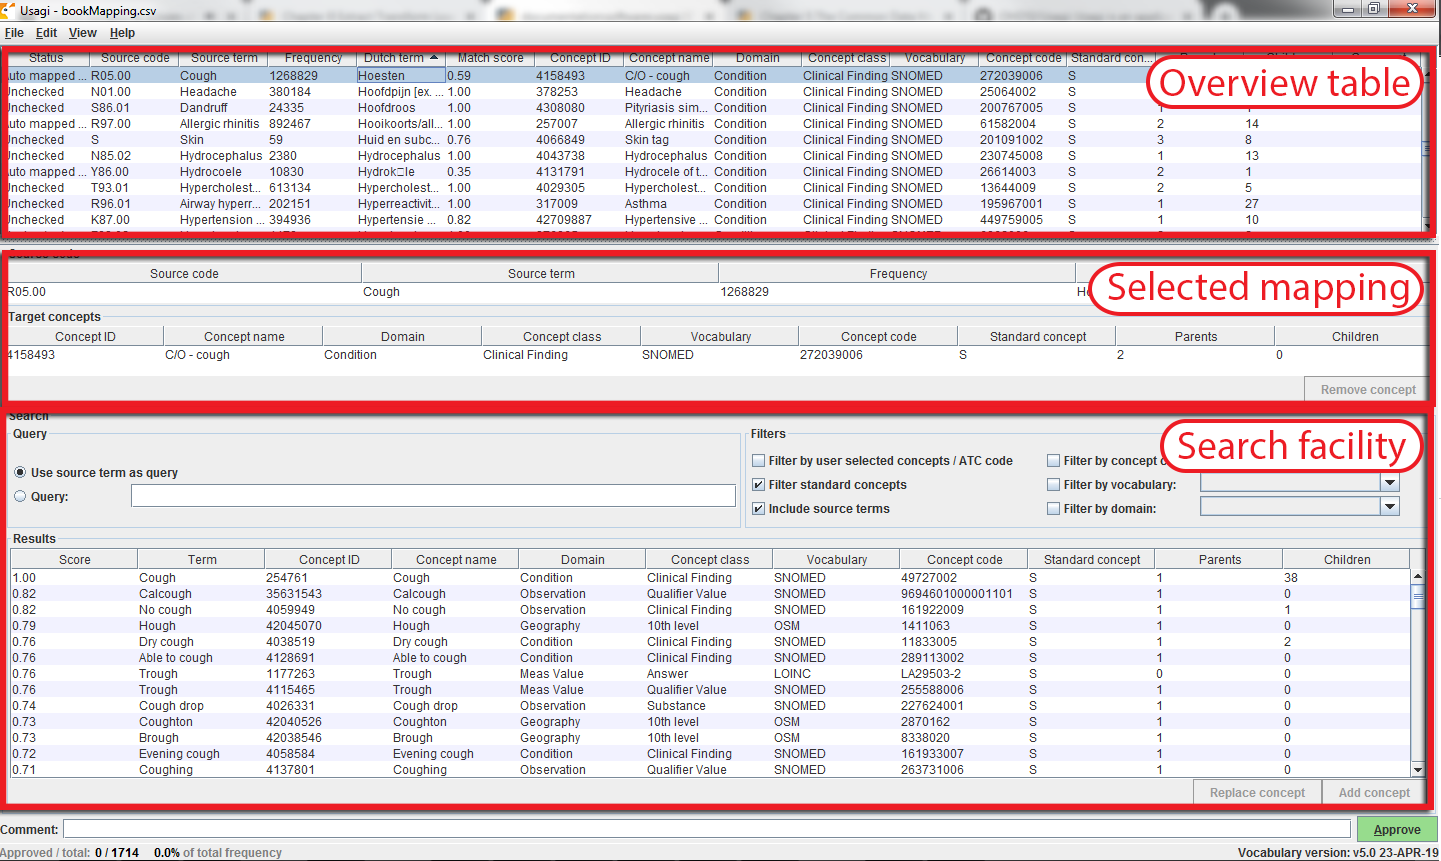
\includegraphics[width=1\linewidth]{images/ExtractTransformLoad/usagiOverview} 

}

\caption{Usagi 소스코드 입력화면.}\label{fig:usagiOverview}
\end{figure}

\subsubsection*{제안된 매핑의 승인}\label{--}
\addcontentsline{toc}{subsubsection}{제안된 매핑의 승인}

``Overview Table''은 현재의 원천 코드의 매핑을 보여준다. 원천 코드를
불러온 직후, 검색 설정과 단어 유사도를 기반으로 자동으로 생성되어 제안된
매핑을 포함하고 있다. 그림 \ref{fig:usagiOverview}에서 나타나듯이,
사용자가 검색 옵션을 Condition으로 설정했기에 네덜란드어 Condition
코드의 영어 이름은 Condition 도메인의 표준용어로 매핑되는 것을 볼 수
있다. Usagi는 원천 코드 기술서의 concept 이름과 동의어를 비교함으로써
최적의 매칭을 수행한다. 사용자가 ``Include source terms''를 선택하였기
때문에 Usagi는 vocabulary의 특정 코드로 매핑되는 모든 원천 코드의 이름과
동의어까지 검토하게 된다. 만약 Usagi가 매핑을 진행할 수 없으면,
CONCEPT\_ID = 0 으로 매핑될 것이다.

코딩 시스템에 익숙한 사람이 원천 코드를 표준 용어로 매핑하는 것을
도와주는 것이 권장된다. 각 개인은 ``Overview Table'' 탭에서 각 코드에
대하여 Usagi가 권장하는 매핑을 받아들이거나 아니면 새로운 매핑을
선택하는 작업을 하게 된다. 예를 들어 그림 \ref{fig:usagiOverview}에서
우리는 네덜란드어 ``Hoesten''가 영어 ``Cough''로 번역되는 것을 볼 수
있다. Usagi는 ``Cough''를 사용하고 Vocabulary 개념 ``4158493-C/O -
cough''로 매핑을 한다. 이때의 매핑에 대하여 매칭 점수는 0.58 (매칭
점수는 일반적으로 0에서 1의 값을 가지며, 1이 더 신뢰할만한 매칭임)
이였고, 이는 Usagi가 이 네덜란드어 코드를 SNOMED로 매핑한 결과에 대한
확신을 가지기 어렵다는 것을 의미한다. 이 예시에서는 해당 매핑 결과에
동의하였고, 화면의 하단 우측의 ``Approve'' 버튼을 클릭함으로써
승인하였다.

\subsubsection*{새로운 매핑의 탐색}\label{--}
\addcontentsline{toc}{subsubsection}{새로운 매핑의 탐색}

Usagi가 제시하는 매핑에 대하여 사용자가 새로운 매핑을 찾거나 아니면
매핑되는 concept이 없도록 (CONCEPT\_ID = 0) 하는 경우들도 있을 것이다.
그림 \ref{fig:usagiOverview}의 예시를 통해 네덜란드어 ``Hoesten''가 영어
``Cough''로 번역되는 것을 확인할 수 있다. Usagi의 제안은 UMLS에서 파생된
매핑으로 제한되기에, 그 결과가 적합하지 않을 수도 있다. 검색 기능을
통해서 실제 용어 자체 혹은 검색 상자 쿼리를 이용해서 다른 concept들을
찾을 수 있다.

매뉴얼 검색 상자를 이용할 때, Usagi는 구조화된 검색 쿼리를 지원하지 않고
fuzzy search를 한다는 것을 기억하여야 한다. 그리고 현재까지는 AND나 OR과
같은 Boolean 연산자를 이용한 검색을 지원하지 않고 있다.

``Cough''에 대해서 더 나은 매핑을 찾는다고 가정해보자. 검색 기능의
오른편 쿼리 부분에 Vocabulary 검색을 할 때 결과를 정리해주는 기능을
제공하는 필터 부분이 있다. 이러한 경우에는 우리는 표준 용어만을 찾아야
하며, 표준 용어에 매핑되는 코드의 이름과 동의어를 기반으로 검색할 수
있다.

이러한 검색 기준을 적용한다면 ``254761-Cough''와 같은 코드를 찾을 수
있으며, 이는 네덜란드어의 코드 매핑에 적합한 용어일 수도 있다. 이를
적용하기 위해 ``Selected Source Code'' 업데이트의 ``Replace concept''
버튼을 누르고, ``Approve'' 버튼을 누르면 된다. 또한 ``Add concept''
버튼이 있는데, 이는 하나의 원천 코드에 대한 다수의 표준 용어 개념 매핑을
할 수 있게 해준다 (예를 들어, 일부 원천 코드들은 표준 용어와는 달리
다양한 질병들을 함께 포함하고 있을 수 있다).

\subsubsection*{개념 정보}\label{-}
\addcontentsline{toc}{subsubsection}{개념 정보}

적절한 개념을 찾아 매핑하려 할 때, concept의 ``social life''를 고려하는
것은 중요하다. 개념의 의미는 계층 구조에서의 위치에 따라 부분적으로
의존적일 수 있으며, 종종 계층적 지위와 거의 혹은 전혀 상관없고 대상
concept으로도 적절하지 않은 ``orphan concepts''들도 있다. Usagi는 각
개념에 대해 얼마나 많은 부모, 자식 개념들이 있는지 알려주기도 하고, ALT
+ C를 누르거나 위쪽 메뉴바의 view -\textgreater{} Concept을 누르면 더
자세한 정보를 볼 수 있게 해준다.

\begin{figure}

{\centering 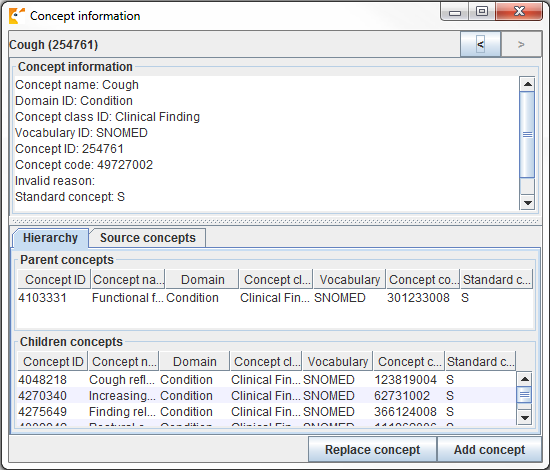
\includegraphics[width=1\linewidth]{images/ExtractTransformLoad/usagiConceptInfo} 

}

\caption{우사기 개념 정보 패널.}\label{fig:usagiConceptInfo}
\end{figure}

그림 \ref{fig:usagiConceptInfo}는 개념 정보 패널을 보여준다. 개념의
일반적인 정보부터, 부모, 자식, 그리고 다른 원천 코드들과의 정보도
보여준다. 사용자는 이 패널을 이용해서 계층 구조를 탐색할 수 있고, 다른
목표 concept을 정할 수도 있다.

모든 코드가 끝날 때까지 코드를 따라 이 절차를 진행하면 된다. 화면의 맨
위의 원천 코드 목록에서, 열 머리글별로 코드들을 정렬할 수 있다. 종종
최고빈도부터 최저빈도의 코드까지 살펴보는 것을 권장한다. 화면의 하단
왼쪽에는 매핑을 허용한 코드들의 개수, 그리고 그에 따라 얼마나 많은
코드가 발생했는지를 확인할 수 있다.

또한 매핑 결정에 대한 설명을 추가하여 문서화 시에 사용할 수도 있다.

\subsubsection*{모범 사례}\label{-}
\addcontentsline{toc}{subsubsection}{모범 사례}

\begin{itemize}
\tightlist
\item
  코딩 스키마에 경험이 있는 사람이 해야 한다.
\item
  ``Overview Table''의 칼럼들을 칼럼 이름을 눌러서 정렬할 수 있다.
  ``Match Score''를 눌러서 정렬하는 것이 중요할 수도 있다; Usagi가 가장
  확실하게 제안하는 매핑 코드들을 검토하면 많은 코드의 작업이 빠르게
  끝날 수도 있다. 그리고 빈도가 높은 단어와 낮은 단어들에 쓰이는 노력이
  각각 다르기 때문에 ``Frequency''로 정렬해서 작업하는 것도 중요하다.
\item
  일부 코드를 CONCEPT\_ID=0 (매핑 안 됨) 으로 매핑하는 것도 허용되며,
  어떤 코드는 좋은 매핑을 찾을 가치가 없어서 일 수도 있고 또는 적절한
  매핑이 없어서 일 수도 있다.
\item
  특히 부모 계층과 자녀 계층에 대해서는 개념의 내용을 고려하는 것이
  중요하다.
\end{itemize}

\subsubsection*{생성된 Usagi Map 내보내기}\label{-usagi-map-}
\addcontentsline{toc}{subsubsection}{생성된 Usagi Map 내보내기}

일단 Usagi를 통해 매핑을 생성하였으면, 이를 사용하기 가장 좋은 방법은
매핑을 내보낸 다음 Vocabulary의 SOURCE\_TO\_CONCEPT\_MAP 테이블에
추가하는 것이다.

매핑을 내보내기 위해서는, File -\textgreater{} Export
source\_to\_concept\_map으로 가면 된다. 이때 어느
SOURCE\_VOCABULARY\_ID를 이용할 것인지 묻는 팝업창이 나타나는데 짧은
식별자를 입력하면 된다. Usagi는 입력된 이 식별자를
SOURCE\_TO\_CONCEPT\_MAP 테이블에서 특정 매핑을 식별할 수 있게 해주는
SOURCE\_VOCABULARY\_ID로 이용할 것이다.

SOURCE\_VOCABULARY\_ID를 선택한 후에는, 내보낼 CSV 파일의 이름과 파일
경로를 입력하게 된다. 내보내는 CSV 파일의 구조는
SOURCE\_TO\_CONCEPT\_MAP 테이블과 동일하다. 이 매핑은 Vocabulary의
SOURCE\_TO\_CONCEPT 테이블로 추가될 수 있다. 그리고 앞선 단계에서 정의한
SOURCE\_VOCABULARY\_ID를 정의하는 VOCABULARY 테이블에 단일 행으로
추가하는 것 역시 가능하다. 마지막으로, ``Approved'' 상태인 매핑들만을
CSV 파일로 내보내는 것이 중요하다; 매핑을 내보내기 위해서는 Usagi에서
매핑을 완료해야만 한다.

\subsubsection*{Usagi Map 업데이트}\label{usagi-map-}
\addcontentsline{toc}{subsubsection}{Usagi Map 업데이트}

매핑은 종종 한 번에 끝나지 않는다. 원천 코드가 추가되는 식으로 데이터가
업데이트되거나 용어가 정기적으로 업데이트되면 매핑 또한 업데이트되어야
할 것이다.

원천 코드가 업데이트될 때는 다음과 같은 단계들을 따르는 것이 좋다:

\begin{enumerate}
\def\labelenumi{\arabic{enumi}.}
\tightlist
\item
  새로운 원천 코드 파일을 불러온다.
\item
  파일을 고른다 -\textgreater{} 이전의 매핑을 적용하고, 예전의 Usagi
  매핑 파일을 선택한다.
\item
  이전의 매핑 파일에서 매핑되지 않았던 코드들을 식별하고, 새롭게
  매핑한다.
\end{enumerate}

용어가 업데이트되면 아래의 단계를 따른다:

\begin{enumerate}
\def\labelenumi{\arabic{enumi}.}
\tightlist
\item
  Athena에서 새로운 용어 파일들을 다운받는다.
\item
  Usagi 인덱스를 다시 생성한다 (Help -\textgreater{} Rebuild index).
\item
  매핑 파일을 연다.
\item
  새로운 용어 버전에 따라 표준 용어가 아닌 코드들을 식별하여 적절한 목표
  concept들을 찾는다.
\end{enumerate}

\section{3단계: ETL 수행}\label{-etl-}

일단 ETL 설계와 코드 매핑이 완료되면, ETL 절차는 소프트웨어를 통해
수행할 수 있다. ETL이 설계될 때, CDM과 원천 데이터 둘 다에 대해 잘 아는
사람이 참여하기를 권장한 바 있다. 마찬가지로 ETL이 수행될 때도, 데이터
(특히 빅데이터) 와 ETL 수행 경험이 있는 사람이 참여하는 것이 바람직하다.
즉, 기관 외부의 기술 전문가를 고용하거나 초청하여 ETL 수행을 시키는 것이
나을 수도 있다. 또한 이 작업은 한 번에 끝나는 작업이 아니라는 점을
참고하기 바란다. 그렇기에 앞으로는 ETL 수행 및 유지에 일정 시간 이상을
할애할 수 있는 사람이나 팀이 있는 것이 좋을 것이다
(\ref{CDMandETLMaintenance}절에서 더 명확히 설명할 것이다).

수행은 각 기관에 따라 다양한 양상을 보이며 특히 정보 인프라,
데이터베이스의 크기, ETL의 복잡성, 기술 전문가의 능력 등의 요소에 따라
많이 달라진다. 많은 요소에 따라 달라지기 때문에 OHDSI는 ETL을 수행하기
위한 최선의 방법에 대한 공식적인 권고를 하고 있지 않다. 그동안 많은
그룹이 SQL builders, SAS, C\#, Java, Kettle들을 사용해왔다. 각각
장점들과 단점들이 있었고, 그 어느 것도 이러한 기술에 익숙한 사람이
없으면 아무것도 사용할 수 없었다.

각각 다른 ETL의 예시들 (복잡성에 따라 정렬된다):

\begin{itemize}
\tightlist
\item
  ETL-Synthea - SQL을 이용한 Synthea 데이터베이스 변환
\item
  \url{https://github.com/OHDSI/etl-synthea}
\item
  ETL-CDMBuilder - 다수의 데이터베이스를 변환하기 위해 고안된 .NET
  application
\item
  \url{https://github.com/OHDSI/etl-cdmbuilder}
\item
  ETL-LambdaBuilder - AWS lamda 기능을 이용한 빌더
\item
  \url{https://github.com/OHDSI/etl-lambdabuilder}
\end{itemize}

그동안 많은 시도가 있었지만, `최종적'인 사용자 친화적 ETL 도구를
개발하는 것은 포기하기로 했다. 항상 많은 경우에 이러한 도구들은 ETL
작업의 80\%까지는 잘 수행하지만, 남은 20\%에 있어서는 원천
데이터베이스에 따라 아래 단에서의 코드 작성이 필요하다.

일단 기술 전문가가 수행할 준비가 된다면, ETL 설계 문서가 그들과
공유되어야만 한다. 문서에는 수행을 시작할만한 충분한 정보가 있어야
하지만, 개발자들이 개발 과정 중에 ETL 설계자들에게 언제나 질문할 수 있는
환경 역시 마련되어 있어야 한다. ETL 설계자들에게는 로직이 명확해
보일지라도 CDM이나 데이터에 친숙하지 않은 수행자들에게는 명확하지 않아
보일 수도 있다. 그렇기에 실행 단계는 팀단위로 수행되어야 한다.
설계자들과 수행자들 모두 로직이 올바르게 작동한다고 동의할 때까지, 모두
CDM 생성과 검증을 같이 수행하는 것이 바람직하다.

\section{4단계: 질 관리}\label{--}

추출, 변환, 적재의 절차 수행을 위해서 질 관리는 반복적으로 수행된다. 질
관리의 전형적인 패턴은 로직 작성 -\textgreater{} 로직 수행
-\textgreater{} 로직 검증 -\textgreater{} 로직 수정 및 작성이다. CDM을
검증하기 위한 많은 방법이 있지만, 아래의 단계들은 몇 년간의 ETL 수행을
통해 OHDSI 내부에서 권고하는 단계들이다. \index{ETL!quality control}

\begin{itemize}
\tightlist
\item
  ETL 설계 문서, 컴퓨터 코드, 코드 매핑을 검토하십시오. 누구라도 실수를
  할 수 있기 때문에, 항상 한 명 이상이 다른 사람이 어떤 작업을 수행하고
  있는지 검토해야 한다.
\item
  컴퓨터 코드의 가장 큰 문제점은 원천 데이터의 원천 코드가 표준 용어에
  어떻게 매핑되었는지에 대한 것이다. 특히 NDC처럼 날짜와 관련 있으면
  매핑이 더욱 어려울 수 있다. 원천 용어가 항상 적절한 개념으로
  변환되도록 매핑이 수행되는 부분을 두 번씩 봐야 한다.
\item
  원천 데이터와 목표 데이터의 표본으로써 특정한 한 사람의 모든 정보를
  수작업으로 비교하십시오.
\item
  여러 개의 기록을 가진 한 사람의 데이터를 살펴보는 것이 큰 도움이 될 수
  있다. 한 사람의 기록을 추적함으로써 CDM 데이터가 로직에 따라 기대했던
  결과와 다른 경우들을 발견해낼 수도 있다.
\item
  원천 데이터와 목표 데이터의 전체 수를 비교하십시오.
\item
  특정 문제들을 어떻게 해결하는지 설명하기에 따라 몇 가지 차이점들이
  있을 수 있다. 예를 들면, 연구자들에 따라 성별이 NULL로 기록된 사람들을
  어차피 연구에 포함되지 않기 때문에 삭제하기로 할 수도 있다. 그리고
  CDM에서의 방문이나 원천 데이터에서의 방문이 다르게 구성될 수도 있다.
  따라서 CDM과 원천 데이터의 총합을 비교할 때는 이러한 차이점들 발생할
  수 있다는 것을 예상하고 설명할 수 있어야 한다.
\item
  해당 CDM 버전에서 원천 데이터에 대해 이미 수행된 기존의 연구를 복제해
  보십시오.
\item
  비록 시간이 많이 들겠지만, 원천 데이터와 CDM 버전에 따른 큰 차이점들을
  확인하기에 좋은 방법이다.
\item
  ETL에서 다뤄야 하는 원천 데이터의 패턴을 따라 하기 위한 단위 검정(Unit
  Test)을 작성하십시오. 예를 들어 만약 ETL 명세에서 성별 정보가 없는
  환자들을 없애야 한다고 명시한다면, 성별이 없는 환자들에 대한 단위
  검정을 작성하고 수행자가 처리하는 방안을 평가하십시오.
\item
  단위 검정은 ETL 변환의 정확도와 질을 평가하기 위한 편리한 방법이다.
  보통은 변환하고자 하는 원천 데이터의 작은 표본을 사용한다. 데이터
  세트의 각 사람이나 기록은 ETL 문서에 기록된 대로 로직의 특정 부분들로
  검정해야 한다. 이 방법을 쓴다면 문제를 파악하거나 로직 실패를
  확인하기에 좋다. 작은 사이즈는 컴퓨터 코드가 훨씬 빠르고 여러 번
  시행하기에도 좋고 에러를 빨리 확인하는데에도 좋다.
\end{itemize}

ETL의 관점에서 고차원의 질 관리 접근법도 있다. 데이터 질 관리에 대한 더
구체적인 노력은 OHDSI에서 진행되고 있으며, \ref{DataQuality}장을
확인해주기 바란다.

\section{ETL 협약 convention과 테미스
THEMIS}\label{etl--convention--themis}

많은 그룹이 데이터를 CDM으로 변환함에 따라 구체적인 협약 convention의
필요성이 명확해졌다. 예를 들어 만약 한 사람의 기록에서 출생연도가 없으면
ETL은 어떻게 할 것인가? CDM의 목적은 보건의료 데이터의 표준화이지만 만약
모든 그룹이 데이터의 특정 시나리오를 각각 다르게 다룬다면 네트워크를
통해 체계적으로 데이터를 다루는 것이 더욱 어려워질 것이다.

OHDSI 공동체는 CDM의 일관성을 증진하기 위해 협약 문서 작성을 시작하였다.
OHDSI가 동의하는 이러한 협약의 정의에 대해서는 CDM wiki를 통해 확인할 수
있다. \footnote{\url{https://github.com/OHDSI/CommonDataModel/wiki}{]}.}
각 CDM 테이블들은 ETL 설계 시 참고할 수 있는 고유의 협약을 맺고 있다.
ETL을 설계할 때 이 협약을 참고한다면 어떤 설계에 대한 결정 시에
커뮤니티와 동일한 일관성을 유지할 수 있도록 도와줄 것이다.

발생 가능한 모든 데이터 시나리오에 대해서 어떻게 다뤄야 할지에 대한
문서를 작성하는 것은 불가능하지만, OHDSI working group을 통해 공통적인
시나리오들을 문서화하는 것은 가능하다. THEMIS\footnote{\url{https://github.com/OHDSI/Themis}}는
협약을 모으고, 명시하고, 공동체에 조언을 나눈 다음, 마지막으로 CDM
wiki에 완성된 문서를 공개하는 일을 하는 각 개인으로 구성되어 있다.
Themis는 고대 그리스의 질서, 공정함, 법, 자연법, 관습을 관장하는
티타니스로 이 그룹의 이름으로 적합해 보인다. ETL을 수행할 때, 만약 특정
시나리오에 대해 어떻게 할지 모르겠다면, THEMIS는 OHDSI 포럼에 질문을
남기기를 권장한다. \footnote{\url{http://forums.ohdsi.org/}} 대부분의
경우 질문에 대해 커뮤니티의 다른 사람들 역시 고민하고 있을 수 있다.
THEMIS는 이런 토론들과 work group 미팅과 대면 토론을 통하여 어떤
협약들이 문서화될 필요가 있는지 알려준다.

\section{CDM과 ETL의 유지}\label{CDMandETLMaintenance}

ETL을 설계하고, 매핑을 만들고, ETL을 수행하고, 질 관리 검증을 만들기는
결코 쉽지 않다. 안타깝게도 그게 다가 아니다. 첫 번째 CDM이 만들어진 후
지속해서 이어지는 ETL 유지 과정이 있다. 유지를 요구하는 몇몇 공통되는
계기는 다음과 같다: 원천 데이터의 변화, ETL 상의 오류, 새로운 OMOP
Vocabulary의 출시, CDM 자체의 변화 혹은 업데이트 등이 있다. 만약 이 중
하나라도 발생한다면, 다음 사항에 대한 업데이트가 필요하다 : ETL 문서,
ETL을 수행한 소프트웨어 프로그래밍, 그리고 예시 검정들과 질 관리

보건의료 데이터들은 보통 계속 바뀐다: 새로운 데이터의 출시 (예를 들어
데이터에 새로운 열의 추가), 기존에 존재하지 않았던 새로운 환자
시나리오의 출현 (예를 들어 출생 전에 사망이 기록되어있는 새로운 환자),
데이터에 대한 이해도의 상승 (예를 들어 입원 아동 환자의 출생 기록이 청구
과정으로 인해 외래에서 발견). 원천 데이터의 모든 변경 사항에 대해서는
아니지만, 최소한 ETL 절차를 망가뜨리는 변경 사항들은 해결해야만 할
것이다.

만약 오류들이 발견된다면 역시 해결해야 할 것이다. 하지만 모든 오류가
동일하게 생성되는 것은 아니라는 것을 염두에 두어야 한다. 예를 들어 COST
테이블에서 비용이 한 자릿수에서 반올림되었다고 가정해보자 (원천
데이터에서 \$3.82가 CDM에서는 \$4.00이 됨). 만약 이 데이터를 사용하는
주요 연구자들이 환자 약물 노출과 진단들에 대한 특성을 주로 연구한다면,
이는 별로 중요하지 않으며 향후 해결하면 된다. 만약 이 데이터를 사용하는
주요 연구자 중 보건경제학자들이 있다면 이는 즉시 해결해야 하는 주요
문제가 될 것이다.

OMOP 용어집 역시 원천 데이터처럼 지속해서 변화한다. 사실용어집은 한 달
안에도 용어들이 업데이트됨에 따라 여러 개의 버전을 가질 수 있다. 각
CDM은 특정 용어집 개별 버전 기반으로 운영되며, 용어집 새 버전에서 작동할
때 원천 코드들이 표준 용어로의 매핑 정도에 따라 다른 결과를 만들 수도
있다. 용어집 간의 차이는 미미할 수도 있지만, 용어집이 개정될 때마다
CDM을 새로 만드는 것은 불필요하다. 하지만, 일 년에 한두 번 정도 새로
출시된 용어집은 기반으로 CDM을 재가공하는 것은 좋을 수 있다. ETL 코드
자체를 새로 업데이트해야 할 정도로 새로운 버전의 용어집이 나오는 일은
매우 드물다.

CDM 또는 ETL 유지를 하게끔 하는 마지막 계기는 공통 데이터 모델 자체의
업데이트이다. 공동체가 커짐에 따라 새로운 데이터의 필요성이 커지고, 이는
CDM에 새로운 데이터를 추가할 수 있는 방향으로 가게 된다. 이는 이전의
CDM에 없었던 데이터가 새로운 버전의 CDM에 들어갈 수 있는 것을 의미한다.
CDM 구조의 변화는 잘 생기지 않지만, 충분히 가능한 일이다. 예를 들어
CDM은 원래의 DATE 필드에서 DATETIME 필드로 적응해갔고, 이는 ETL 절차에서
에러를 발생시킬 수 있는 일이다. CDM 버전은 자주 출시되지 않으며, 각
기관은 데이터를 옮길 때 결정할 수 있다.

\section{ETL에 대한 마지막 생각}\label{etl---}

ETL 절차는 여러 가지 이유로 완전히 통달하기 어려운 절차이다. 각자가 서로
다른 고유한 원천 데이터를 다루기 때문에 ``만능열쇠''를 만드는 것은
어렵다. 하지만, 수년간 시도에서 배운 몇 가지 교훈이 있다.

\begin{itemize}
\tightlist
\item
  80/20 규칙. 피할 수만 있다면 너무 많은 시간을 원천 코드를 표준개념으로
  수동 매핑하는데 할애하지 마십시오. 전체 데이터양의 대부분을 차지하는
  원천 코드만 매핑하는 것이 이상적이다. 그것만으로도 시작하기에 충분할
  것이고, 실제 사용 예시에 기반하여 나머지 남은 코드들도 다룰 수 있다.
\item
  연구 품질에 맞지 않는 데이터를 잃어버리는 것은 괜찮다. 이런 기록들은
  분석을 시작하기 전에 결국은 버려지게 되고, 우리는 대신 ETL 절차에서
  미리 삭제할 뿐이다.
\item
  CDM은 유지를 필요로 한다. 단순히 ETL을 완료했다는 것은 두 번 다시
  손대지 않는 것을 의미하는 것이 아니다. 원천 데이터는 변할 수도 있고,
  코드에 오류가 있을 수도 있고, 새로운 용어가 나오거나 CDM에 업데이트가
  있을 수 있다. 이러한 변화에 대비하고 ETL을 최신 상태로 유지하기 위해
  자원을 할당할 필요가 있다.
\item
  OHDSI CDM으로 시작하는 것을 돕고, 데이터베이스의 변환을 수행하거나
  분석 도구를 사용하기 위해 Implementers Forum에 방문해주길 바란다.
  \footnote{\url{https://forums.ohdsi.org/c/implementers}}
\end{itemize}

\section{요약}\label{-4}

\BeginKnitrBlock{rmdsummary}
\begin{itemize}
\item
  ETL에 접근하는 방법에 대해 일반적으로 합의된 절차들이 있는데 다음과
  같다.
\item
  데이터 전문가와 CDM 전문가가 함께 ETL을 설계한다.
\item
  의료 지식이 있는 사람들이 코드 매핑을 진행한다.
\item
  기술 전문가가 ETL을 수행한다.
\item
  모든 사람이 질 관리에 참여한다.
\item
  이러한 단계들을 돕기 위해 OHDSI 공동체에서 무료로 사용 가능한 도구들을
  개발하였다.
\item
  많은 ETL 예시들이 있으며, 가이드로 삼을만한 협약들이 있다.
\end{itemize}
\EndKnitrBlock{rmdsummary}

\section{예제}\label{-2}

\BeginKnitrBlock{exercise}
\protect\hypertarget{exr:exerciseEtl1}{}{\label{exr:exerciseEtl1} }다음 ETL
절차들을 올바른 단계로 정렬하십시오:

\begin{enumerate}
\def\labelenumi{\Alph{enumi})}
\tightlist
\item
  데이터 전문가와 CDM 전문가가 함께 ETL을 설계한다.
\item
  기술 전문가가 ETL을 수행한다.
\item
  의료 지식이 있는 사람들이 코드 매핑을 진행한다.
\item
  모든 사람이 질 관리에 참여한다.
\end{enumerate}
\EndKnitrBlock{exercise}

\BeginKnitrBlock{exercise}
\protect\hypertarget{exr:exerciseEtl2}{}{\label{exr:exerciseEtl2} }선택한
OHDSI 자원을 활용하여, 테이블 \ref{tab:exercisePersonTable}의 PERSON
기록에서 나타나는 4가지 문제들을 발견하십시오 (공간상 축약된 형태의 표):

\begin{longtable}[]{@{}ll@{}}
\caption{\label{tab:exercisePersonTable} A PERSON table.}\tabularnewline
\toprule
Column & Value\tabularnewline
\midrule
\endfirsthead
\toprule
Column & Value\tabularnewline
\midrule
\endhead
PERSON\_ID & A123B456\tabularnewline
GENDER\_CONCEPT\_ID & 8532\tabularnewline
YEAR\_OF\_BIRTH & NULL\tabularnewline
MONTH\_OF\_BIRTH & NULL\tabularnewline
DAY\_OF\_BIRTH & NULL\tabularnewline
RACE\_CONCEPT\_ID & 0\tabularnewline
ETHNICITY\_CONCEPT\_ID & 8527\tabularnewline
PERSON\_SOURCE\_VALUE & A123B456\tabularnewline
GENDER\_SOURCE\_VALUE & F\tabularnewline
RACE\_SOURCE\_VALUE & WHITE\tabularnewline
ETHNICITY\_SOURCE\_VALUE & NONE PROVIDED\tabularnewline
\bottomrule
\end{longtable}
\EndKnitrBlock{exercise}

\BeginKnitrBlock{exercise}
\protect\hypertarget{exr:exerciseEtl3}{}{\label{exr:exerciseEtl3}
}VISIT\_OCCURRENCE 기록들을 만들어보자. Synthea에 대한 예시 로직이
다음과 같이 있다: PATIENT, START, END에 따라 오름차순으로 데이터를
정렬하십시오. 그다음 PERSON\_ID 별로, 하나의 기록의 END 시간과 다음
기록의 START 시간의 차이가 1일 이하인 기록들을 하나로 만들어 준다. 각
통합된 입원 환자 기록들은 하나의 입원 환자 방문으로 간주하며, 다음과
같이 설정한다:

\begin{itemize}
\tightlist
\item
  MIN(START) as VISIT\_START\_DATE
\item
  MAX(END) as VISIT\_END\_DATE
\item
  ``IP'' as PLACE\_OF\_SERVICE\_SOURCE\_VALUE
\end{itemize}

만약 아래와 같은 그림 \ref{fig:exerciseSourceData}의 방문 기록들이 원천
데이터라고 가정한다면, CDM에서의 VISIT\_OCCURRENCE 기록은 어떻게 보일
것인가?
\EndKnitrBlock{exercise}

\begin{figure}

{\centering 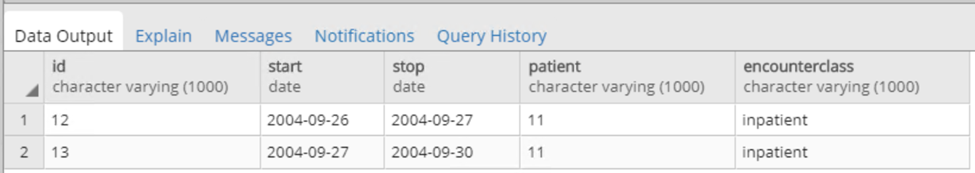
\includegraphics[width=1\linewidth]{images/ExtractTransformLoad/exerciseSourceData} 

}

\caption{원천 데이터 예시.}\label{fig:exerciseSourceData}
\end{figure}

제안된 답변은 부록 \ref{Etlanswers}에서 확인할 수 있다.

\part{Data Analytics}\label{part-data-analytics}

\chapter{데이터 분석 이용 사례}\label{DataAnalyticsUseCases}

\emph{Chapter lead: David Madigan}

OHDSI는 실세계 헬스케어 데이터 (일반적으로 보험청구 또는 의무기록
데이터베이스) 로부터 믿을만한 근거를 만들어내는 데 초점을 맞춰 왔다.
OHDSI가 관심을 가져온 이용 사례들은 크게 3개의 카테고리로 구분된다:

\begin{itemize}
\tightlist
\item
  특성 분석
\item
  인구 수준 추정
\item
  환자 수준 예측
\end{itemize}

본 장에서는 각 카테고리에 관해 설명한다. 모든 이용 사례들에 있어서,
생성된 근거들은 데이터 자체가 가지고 있는 한계를 이어받는다는 점을
유념하십시오. 이 한계들에 대해서는 이 책의 ``근거의 질'' 장에서 다루고
있다. (\ref{EvidenceQuality}장 \textasciitilde{} \ref{MethodValidity}장)

\section{특성 분석}\label{-}

\index{characterization}

특성 분석은 다음과 같은 질문에 답변을 시도한다.

\begin{quote}
그들에게 무슨 일이 발생했는가?
\end{quote}

우리는 데이터를 이용하여 코호트 또는 전체 데이터베이스 내 환자들과
헬스케어의 특성을 묻는 말에 답할 수 있으며, 시간이 지남에 따라 이
특성들이 어떻게 변화하는지 알 수 있다.

데이터는 다음과 같은 질문에 답을 제공할 수 있다:

\begin{itemize}
\tightlist
\item
  심방세동으로 새 진단을 받은 환자 중 얼마나 많은 사람이 와파린을
  처방받는가?
\item
  고관절 치환술을 받은 환자들의 평균 연령은 어떻게 되는가?
\item
  65세 이상 환자 중 폐렴 발생률은 얼마나 되는가?
\end{itemize}

일반적인 특성 분석 질문들은 다음과 같이 표현된다:

\begin{itemize}
\tightlist
\item
  얼마나 많은 환자가\ldots{}?
\item
  얼마나 자주\ldots{}?
\item
  환자 중 어느 정도의 비율이\ldots{}?
\item
  \ldots{} 검사에 대한 결과값의 분포가 어떠한가?
\item
  \ldots{} 질병을 가진 환자들의 당화혈색소(HbA1c) 수준이 어떠한가?
\item
  \ldots{} 환자들에 대한 검사 결과값이 어떠한가?
\item
  환자가 \ldots{}에 노출되는 평균 노출 기간은 얼마인가?
\item
  \ldots{}의 시간 경과에 따른 추세는 무엇인가?
\item
  이 환자들이 사용하는 다른 약들이 무엇인가?
\item
  수반되는 치료법들이 무엇인가?
\item
  \ldots{}에 대한 충분한 증례가 있는가?
\item
  \ldots{}에 대한 연구 X가 실행 가능한가?
\item
  \ldots{}에 대한 인구통계학적 특징은 무엇인가?
\item
  \ldots{}의 위험인자들이 무엇인가? (특정 위험인자가 구분된다면, 이는
  예측이 아닌 추정에 해당함)
\item
  \ldots{}의 예측요인들이 무엇인가?
\end{itemize}

그리고 원하는 결과값은 다음과 같다:

\begin{itemize}
\tightlist
\item
  건수 또는 퍼센트(count or percentage)
\item
  평균(averages)
\item
  기술 통계(descriptive statistics)
\item
  발생률(incidence rate)
\item
  유병률(prevalence)
\item
  코호트(cohort)
\item
  규칙 기반 표현형(rule-based phenotype)
\item
  약물 사용(drug utilization)
\item
  질병의 자연 경과(disease natural history)
\item
  순응도(adherence)
\item
  동반 질환 프로파일(co-morbidity profile)
\item
  치료 경로(treatment pathways)
\item
  치료 요법(line of therapy)
\end{itemize}

\section{인구 수준 추정}\label{--}

\index{population-level estimation}

제한된 범위내에서, 데이터는 헬스케어 개입 효과에 대한 인과적 추론을
지원함으로써 질문에 답할 수 있다.

\begin{quote}
무엇이 인과 효과 causal effect인가?
\end{quote}

우리는 행동의 결과를 이해하기 위해 인과 효과를 파악하고자 한다. 예를
들어, 우리가 어떤 치료법을 사용하기로 했다면, 이것이 앞으로 우리에게
무슨 변화를 일으킬까?

데이터는 다음과 같은 질문에 답을 줄 수 있다:

\begin{itemize}
\tightlist
\item
  새로 심방세동으로 진단받은 환자들에 있어서, 치료 시작한 지 1년 이내에
  와파린 warfarin이 다비가트란 dabigatran 보다 주요 출혈을 더
  일으키는가?
\item
  메트포르민 metformin이 설사에 미치는 인과 효과가 연령에 따라 다른가?
\end{itemize}

일반적인 인구 수준 효과 추정 질문들은 다음과 같이 표현된다:

\begin{itemize}
\tightlist
\item
  \ldots{}의 효과는 무엇인가?
\item
  내가 개입한다면 어떻게 될까\ldots{}?
\item
  어떤 치료가 더 효과가 좋을까?
\item
  X가 Y에 미치는 위험이 무엇일까?
\item
  \ldots{} 이벤트 발생에 걸리는 시간 time-to-event가 얼마나 될까?
\end{itemize}

그리고 원하는 결과값은 다음과 같다:

\begin{itemize}
\tightlist
\item
  상대 위험도(relative risk)
\item
  발생 위험비(hazards ratio)
\item
  대응위험도/교차비(odds ratio)
\item
  평균 처치 효과(average treatment effect)
\item
  인과적 영향(causal effect)
\item
  관련성(association)
\item
  상관성(correlation)
\item
  안전성 감시(safety surveillance)
\item
  비교 효과(comparative effectiveness)
\end{itemize}

\section{환자 수준 예측}\label{--}

\index{patient-level prediction}

데이터베이스에 쌓인 환자 건강 이력을 기반으로, 우리는 미래에 발생할 건강
이벤트에 대해 환자 수준의 예측할 수 있다.

\begin{quote}
나에게 무슨 일이 발생할까?
\end{quote}

데이터는 다음과 같은 질문에 답을 제공할 수 있다:

\begin{itemize}
\tightlist
\item
  주요 우울증으로 새롭게 진단받은 특정 환자가 진단받은 지 1년 안에
  자살을 시도할 확률이 얼마나 되는가?
\item
  심방세동으로 새롭게 진단받은 특정 환자가, 와파린으로 치료를 시작한 지
  1년 안에 허혈성 뇌졸중을 겪을 확률이 얼마나 되는가?
\end{itemize}

일반적인 환자 수준 예측에 대한 질문들은 다음과 같이 표현된다:

\begin{itemize}
\tightlist
\item
  이 환자가 \ldots{}할 가능성이 얼마나 되는가?
\item
  \ldots{}에 대한 후보자들이 누구인가?
\end{itemize}

그리고 원하는 결과값은 다음과 같다:

\begin{itemize}
\tightlist
\item
  개인에 대한 확률
\item
  예측 모델
\item
  높은/낮은 위험군
\item
  확률론적 표현형
\end{itemize}

인구 수준 추정과 환자 수준 예측은 어느 정도 중복된다. 예측을 위한 중요
이용사례로 다음 예제를 들 수 있다: 약물 A가 처방된 특정 환자의 임상
결과를 예측하는 것과 또한 약물 B가 처방된 사람에게서 그와 똑같은 임상
결과를 예측하는 것이다. 실제로 한 환자가 여러 약 중 하나 (약물 A이라고
하자) 를 처방받았고, 약물 A의 예상되는 결과가 실제로 일어나는지를
살펴봤다고 가정해 보자. 그 환자에게 약물 B는 처방되지 않았고 B 투여
이후의 임상 결과는 관찰된 적이 없으므로 그 예상된 임상 결과는 반 사실적
(counterfactual)이며, 예측은 할 수 있더라도 사실과 다를 수 있다. 이러한
각각의 예측 작업은 환자 수준 예측에 속한다. 그러나 두 결과의 차이 (또는
비율) 는 단위 수준의 \emph{인과} 효과이며, 예측모형이 아닌 인과적 영향
추정 방법론을 사용하여 추정하여야 한다.

\BeginKnitrBlock{rmdimportant}
사람들은 예측모델을 인과 모델로 잘못 해석하는 경향이 있다. 그러나 예측
모델은 상관성만을 보여줄 수 있으며 결코 인과성을 보여줄 수 없다. 예를
들자면, 당뇨병이 심근경색의 강한 예측변수이기 때문에, 당뇨병 약을
사용하는 것은 심근경색의 강한 예측변수일 수 있다. 그러나 이것이 당뇨병
약 복용을 중단하는 것이 심근경색을 막는다는 것을 의미하는 것은 아니다!
\EndKnitrBlock{rmdimportant}

\section{고혈압 이용 사례 예}\label{---}

당신은 고혈압의 1차 치료 요법으로서 ACE 억제제 단일요법과 타이아자이드
이뇨제 단일요법이 급성 심근경색과 혈관부종에 미치는 영향을 연구하는 데
관심이 있는 연구자이다. 당신은 OHDSI 연구에 기반하여 인구 수준 추정 연구
질문을 도출했지만, 먼저 관심이 있는 특정 치료에 대한 특성을 어떻게
분석할 것인지 해결해야 한다.

\subsection{특성 분석 질문}\label{--}

급성 심근경색은 고혈압 환자들에게 일어날 수 있는 심혈관계 합병증으로,
고혈압에 대한 효과적인 치료로 이 위험을 줄여야 한다. 혈관부종은
희귀하지만, 잠재적으로 심각한 ACE 억제제의 알려진 부작용이다. 당신은
관심 약제 (ACE 억제제와 티아자이드 이뇨제) 들에 노출된 코호트
(\ref{Cohorts}장 참고) 를 생성하는 것으로부터 연구를 시작한다. 노출된
환자들의 인구통계학적 정보, 병적 상태, 병용 약물 등 기저 특성을 파악하기
위하여 특성 분석 (\ref{Characterization}장 참고) 을 수행한다. 또한 이
노출 환자 내에서 분석하고자 하는 결과가 얼마나 발생하는지 추정하는 또
다른 특성 분석을 수행한다. 그리고, 당신은 `얼마나 자주 1) 급성
심근경색과 2) 혈관부종이 ACE 억제제와 티아자이드 이뇨제에 노출된 기간
동안 발생하는가?'를 묻게 된다. 이러한 특성 분석은 인구 수준 추정 연구
수행의 실현 가능성을 판단하게 하고, 두 치료군이 비교 가능한지를 평가하게
하며, 환자들이 받는 치료에 예측되는 위험 요소들을 파악할 수 있게 한다.

\subsection{인구 수준 추정에 대한 질문}\label{----}

인구 수준 효과 추정 연구 (\ref{PopulationLevelEstimation}장 참고) 는 ACE
억제제와 티아자이드 이뇨제가 급성 심근경색과 혈관부종에 미치는 상대
위험을 추정한다. 더 나아가, 분석에 대한 평가와 음성대조군 분석을 통해
우리가 평균 치료 효과에 대해 믿을 만한 추정치를 도출했는지 평가한다.

\subsection{환자 수준 예측에 대한 질문}\label{----}

당신은 노출의 인과적 영향 여부와 상관없이, 가장 위험한 결과에 처한
환자들을 알아내고자 할 수 있다. 이것은 환자 수준 예측
(\ref{PatientLevelPrediction}장 참고) 의 문제이다. ACE 억제제를 처음
사용하는 환자 중 치료 시작한 지 1년 동안 급성 심근경색 발병 위험이 가장
높은 환자들을 찾아내는 예측 모델을 개발한다고 생각해 보십시오. 이 모델을
통해 우리는 처음으로 ACE 처방을 받은 환자의 병력에서 관찰된 사건을
바탕으로, 향후 1년 동안 급성 심근경색을 겪을 가능성을 예측할 수 있다.

\section{관찰 연구의 한계}\label{--}

\index{limitations of obervational research}

OHDSI 데이터베이스가 답변을 제공할 수 없는 중요한 의료분야 질문들이 많이
존재한다. 아래 질문들이 이에 해당한다:

\begin{itemize}
\tightlist
\item
  위약과 비교한 치료의 인과 효과. 때때로 치료군의 인과 효과를 비치료군과
  비교하여 분석하는 것은 고려해 볼 수 있지만 위약군과 비교하려고 해서는
  안 된다.
\item
  처방전 없이 구입할 수 있는 일반 의약품과 관련된 모든 것
\item
  많은 임상 결과와 여러 변수가 아주 성기게 기록된 경우. 사망률, 행동
  결과, 라이프 스타일 및 사회-경제적 지위와 같은 것들이 이에 포함된다.
\item
  환자는 건강이 좋지 않을 때만 의료 시스템을 이용하는 경향이 있기
  때문에, 치료의 이점을 측정하기가 쉽지 않다.
\end{itemize}

\subsection{잘못된 데이터}\label{-}

OHDSI 데이터베이스에 기록된 임상 데이터는 의료 현실과 차이가 있을 수
있다. 예를 들어, 환자가 심근경색을 경험한 적이 없어도 환자의 기록에
심근경색 코드가 포함되어 있을 수 있다. 마찬가지로 검사 값이 잘못되었거나
시술에 대한 잘못된 코드가 데이터베이스에 저장되었을 수도 있다.
\ref{DataQuality}장과 \ref{ClinicalValidity}장은 이와 같은 이슈들을
다루고 있으며, 모범 사례를 통해 이러한 문제들을 최대한 식별하고
수정하고자 한다. 그런데도, 잘못된 데이터는 필연적으로 어느 정도까지
존재할 수밖에 없으며, 분석의 타당성을 약화시킬 수 있다. 매우 많은 문헌이
데이터 오류들을 처리하기 위한 통계적 추론 보정에 초점을 맞추고 있다. -
예를 들어 \citet{fuller2009measurement} 참조

\subsection{결측 데이터}\label{-}

\index{missing data}

OHDSI 데이터베이스에서의 결측은 감지하기 어려운 문제점들을 낳는다.
데이터베이스에 기록되어야 하는 건강 이벤트 (예를 들어 처방, 검사 값 등)
가 기록되지 않은 것, 그것이 ``결측''이다. 통계 문헌들은 ``임의의 완전
결측'', ``임의의 결측'', ``임의가 아닌 결측''과 같은 결측 유형들과
이러한 유형들을 다루는 복잡한 방법론들을 구별하고 있다.
\citet{perkins2017principled} 가 이 주제에 대한 유용한 입문서를
제공한다.

\section{요약}\label{-5}

\BeginKnitrBlock{rmdsummary}
\begin{itemize}
\item
  관찰 연구의 이용 사례들은 크게 3개의 카테고리로 구분된다.
\item
  \textbf{특성 분석}은 ``그들에게 무슨 일이 발생했는가?''라는 질문에
  답하는 것을 목적으로 한다.
\item
  \textbf{인구 수준 추정}은 ``인과적 영향이 무엇인가?''라는 질문에
  답하는 것을 목적으로 한다.
\item
  \textbf{환자 수준 예측}은 ``나에게 무엇이 일어날까?''라는 질문에
  답하는 것을 목적으로 한다.
\item
  예측 모델은 인과 모델이 아니다; 강한 예측변수를 통제하는 것이 결과에
  영향을 미칠 것이라고 믿을 근거가 없다.
\item
  관찰형 의료 데이터를 이용하여 연구할 수 없는 질문들도 있다.
\end{itemize}
\EndKnitrBlock{rmdsummary}

\section{예제}\label{-3}

\BeginKnitrBlock{exercise}
\protect\hypertarget{exr:exerciseUseCases1}{}{\label{exr:exerciseUseCases1}
}다음 질문들은 어떤 사용 사례 카테고리에 해당하는가?

\begin{enumerate}
\def\labelenumi{\arabic{enumi}.}
\item
  비스테로이드 약물에 최근 노출되었던 환자들이 위장관 출혈을 겪을 비율을
  계산하십시오.
\item
  기저 특성을 기반으로 특정 환자가 차년도에 위장관 출혈을 겪을 확률을
  계산하십시오.
\item
  셀레콕시브 celecoxib와 비교하여 디클로페낙 diclofenac이 위장관 출혈에
  미치는 위험을 추정하십시오.
\end{enumerate}
\EndKnitrBlock{exercise}

\BeginKnitrBlock{exercise}
\protect\hypertarget{exr:exerciseUseCases2}{}{\label{exr:exerciseUseCases2}
}당신은 디클로페낙 diclofenac이 위장관 출혈에 미치는 위험을 비노출
(위약) 의 경우와 비교하여 추정하고자 한다. 이와 같은 연구가 헬스케어
관찰 데이터를 이용하여 수행 가능한가?
\EndKnitrBlock{exercise}

제안된 답변은 부록 \ref{UseCasesanswers}에서 확인할 수 있다.

\chapter{OHDSI 분석 툴}\label{OhdsiAnalyticsTools}

\emph{Chapter leads: Martijn Schuemie \& Frank DeFalco}

OHDSI는 관찰 환자 수준 데이터에 대한 다양한 데이터 분석 사용 사례를
지원하는 광범위한 오픈 소스 도구를 제공한다. 이러한 도구의 공통점은 공통
데이터 모델(CDM)을 사용하여 하나 이상의 데이터베이스와 상호 작용할 수
있다는 것이다. 또한, 이러한 도구는 다양한 사용 사례 use case에 대한
분석을 표준화한다. 처음부터 시작하는 것이 아니라 표준 템플릿을
작성함으로써 분석을 구현할 수 있다. 이렇게 하면 분석을 더 쉽게 수행할 수
있고, 재현성과 투명성을 향상할 수 있다. 예를 들어, 발생률을 계산하는
방법은 무한에 가까운 수가 있는 것처럼 보이지만, 이러한 방법은 몇 가지
선택사항으로 OHDSI 도구에 지정할 수 있으며, 동일한 선택을 하는 사람은
동일한 방법으로 발병률을 계산할 것이다.

이 장에서는 먼저 분석을 실행하기 위해 선택할 수 있는 다양한 방법과
분석에서 어떤 전략을 사용할 수 있는지 설명한다. 그런 다음 다양한 OHDSI
툴과 다양한 사용 사례에 적합한 방법을 검토한다.

\section{분석 구현}\label{analysisImplementation}

그림 \ref{fig:implementations}은 CDM을 사용하여 데이터베이스에 대한
연구를 구현하도록 선택할 수 있는 다양한 방법을 보여준다.
\index{analysis implementation}

\begin{figure}

{\centering 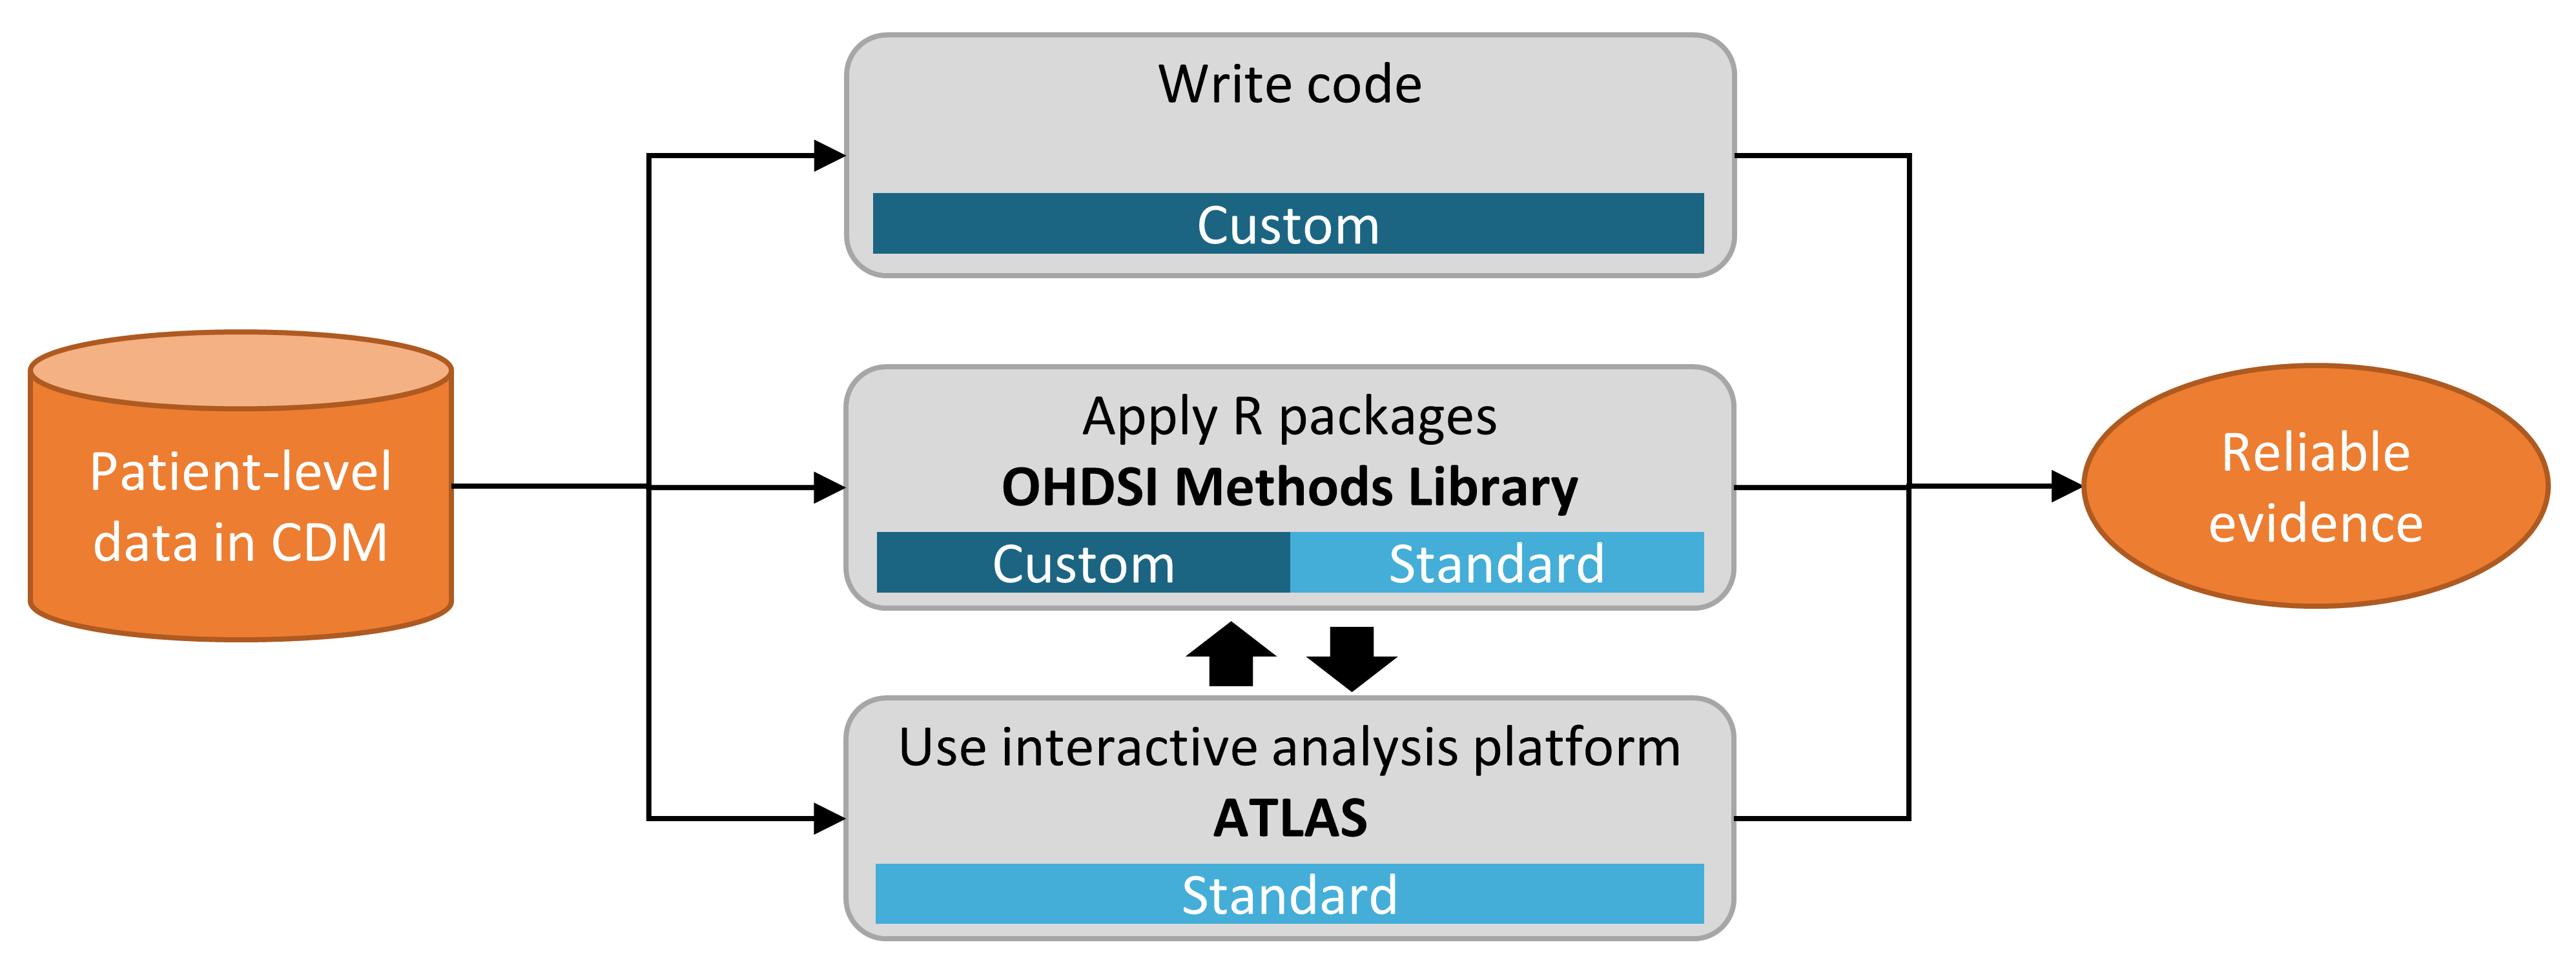
\includegraphics[width=0.9\linewidth]{images/OhdsiAnalyticsTools/implementations} 

}

\caption{CDM의 데이터에 대한 분석을 구현하는 다양한 방법}\label{fig:implementations}
\end{figure}

연구를 이행하는 데는 세 가지 주요 접근법이 있다. 첫 번째는 OHDSI가
제공하는 어떤 도구도 사용하지 않고 사용자가 직접 코드를 작성하는 것이다.
R, SAS 또는 다른 언어로 새로운 분석코드를 작성할 수 있다. 이는 최대의
유연성을 제공하며, 특정 분석이 우리의 툴에 의해 뒷받침되지 않는 경우
사실상 유일한 선택사항이 될 수 있다. 그러나 이러한 경로에는 많은 전문적
기술과 시간, 노력이 필요하며, 분석의 복잡성이 증가함에 따라 코드의
오류를 피하기 어려워진다.

두 번째 접근방식은 R을 이용하고,
\href{https://ohdsi.github.io/MethodsLibrary/}{OHDSI Methods Library}의
패키지를 이용하는 것이다. 최소한 \ref{SqlAndR}장에 설명된
\href{https://ohdsi.github.io/SqlRender/}{SqlRender} 및
\href{https://ohdsi.github.io/DatabaseConnector/}{DatabaseConnector}
패키지를 사용하여 PostgreSQL, SQL Server, 그리고 Oracle과 같은 다양한
데이터베이스 플랫폼에서 동일한 코드를 실행할 수 있다.
\href{https://ohdsi.github.io/CohortMethod/}{CohortMethod}와
\href{https://ohdsi.github.io/PatientLevelPrediction/}{PatientLevelPrediction}과
같은 다른 패키지는 자신의 코드로 호출할 수 있는 CDM에 대한 고급 분석을
위한 R 기능을 제공한다. 이것은 여전히 많은 기술적 전문지식이 필요하지만,
Methods Library의 검증된 구성요소를 다시 사용함으로써 사용자가 모든
코드를 다 짜는 것 보다 더 효율적이고 오류가 덜 발생할 수 있다.

세 번째 접근법은 프로그래머가 아닌 사람들이 다양한 분석을 효율적으로
수행할 수 있도록 해주는 웹 기반 툴인 대화형 분석 플랫폼
\href{https://github.com/OHDSI/Atlas/wiki}{ATLAS}에 의존한다. ATLAS는
Method Libraries를 사용하지만, 분석을 설계하기 위한 간단한 그래픽
인터페이스를 제공하며 많은 경우 분석을 실행하는 데 필요한 R 코드를
생성한다. 그러나 ATLAS는 Methods Library에서 사용할 수 있는 모든 옵션을
다 지원하지는 않는다. 대부분의 연구가 ATLAS를 통해 수행될 수 있을 것으로
예상되지만, 일부 연구는 두 번째 접근방식이 제공하는 유연성을 필요로 할
수 있다.

ATLAS와 Methods Library는 독립적이지 않다. ATLAS에서 호출할 수 있는 더
복잡한 분석 중 일부는 Methods Library의 패키지에 대한 호출을 통해
실행된다. 마찬가지로 Methods Library에 사용되는 코호트는 ATLAS에서
설계되는 경우가 많다.

\section{분석 전략}\label{-}

사용자 정의 코드를 사용하거나 Methods Library의 표준 분석 코드를
사용하여 CDM에 대한 분석을 구현하는 것 외에도, 그러한 분석 기법을
사용하여 근거를 생성하는 데에는 여러 가지 전략이 있다. 그림
\ref{fig:strategies}은 OHDSI에 채택된 세 가지 전략을 보여준다.

\begin{figure}

{\centering 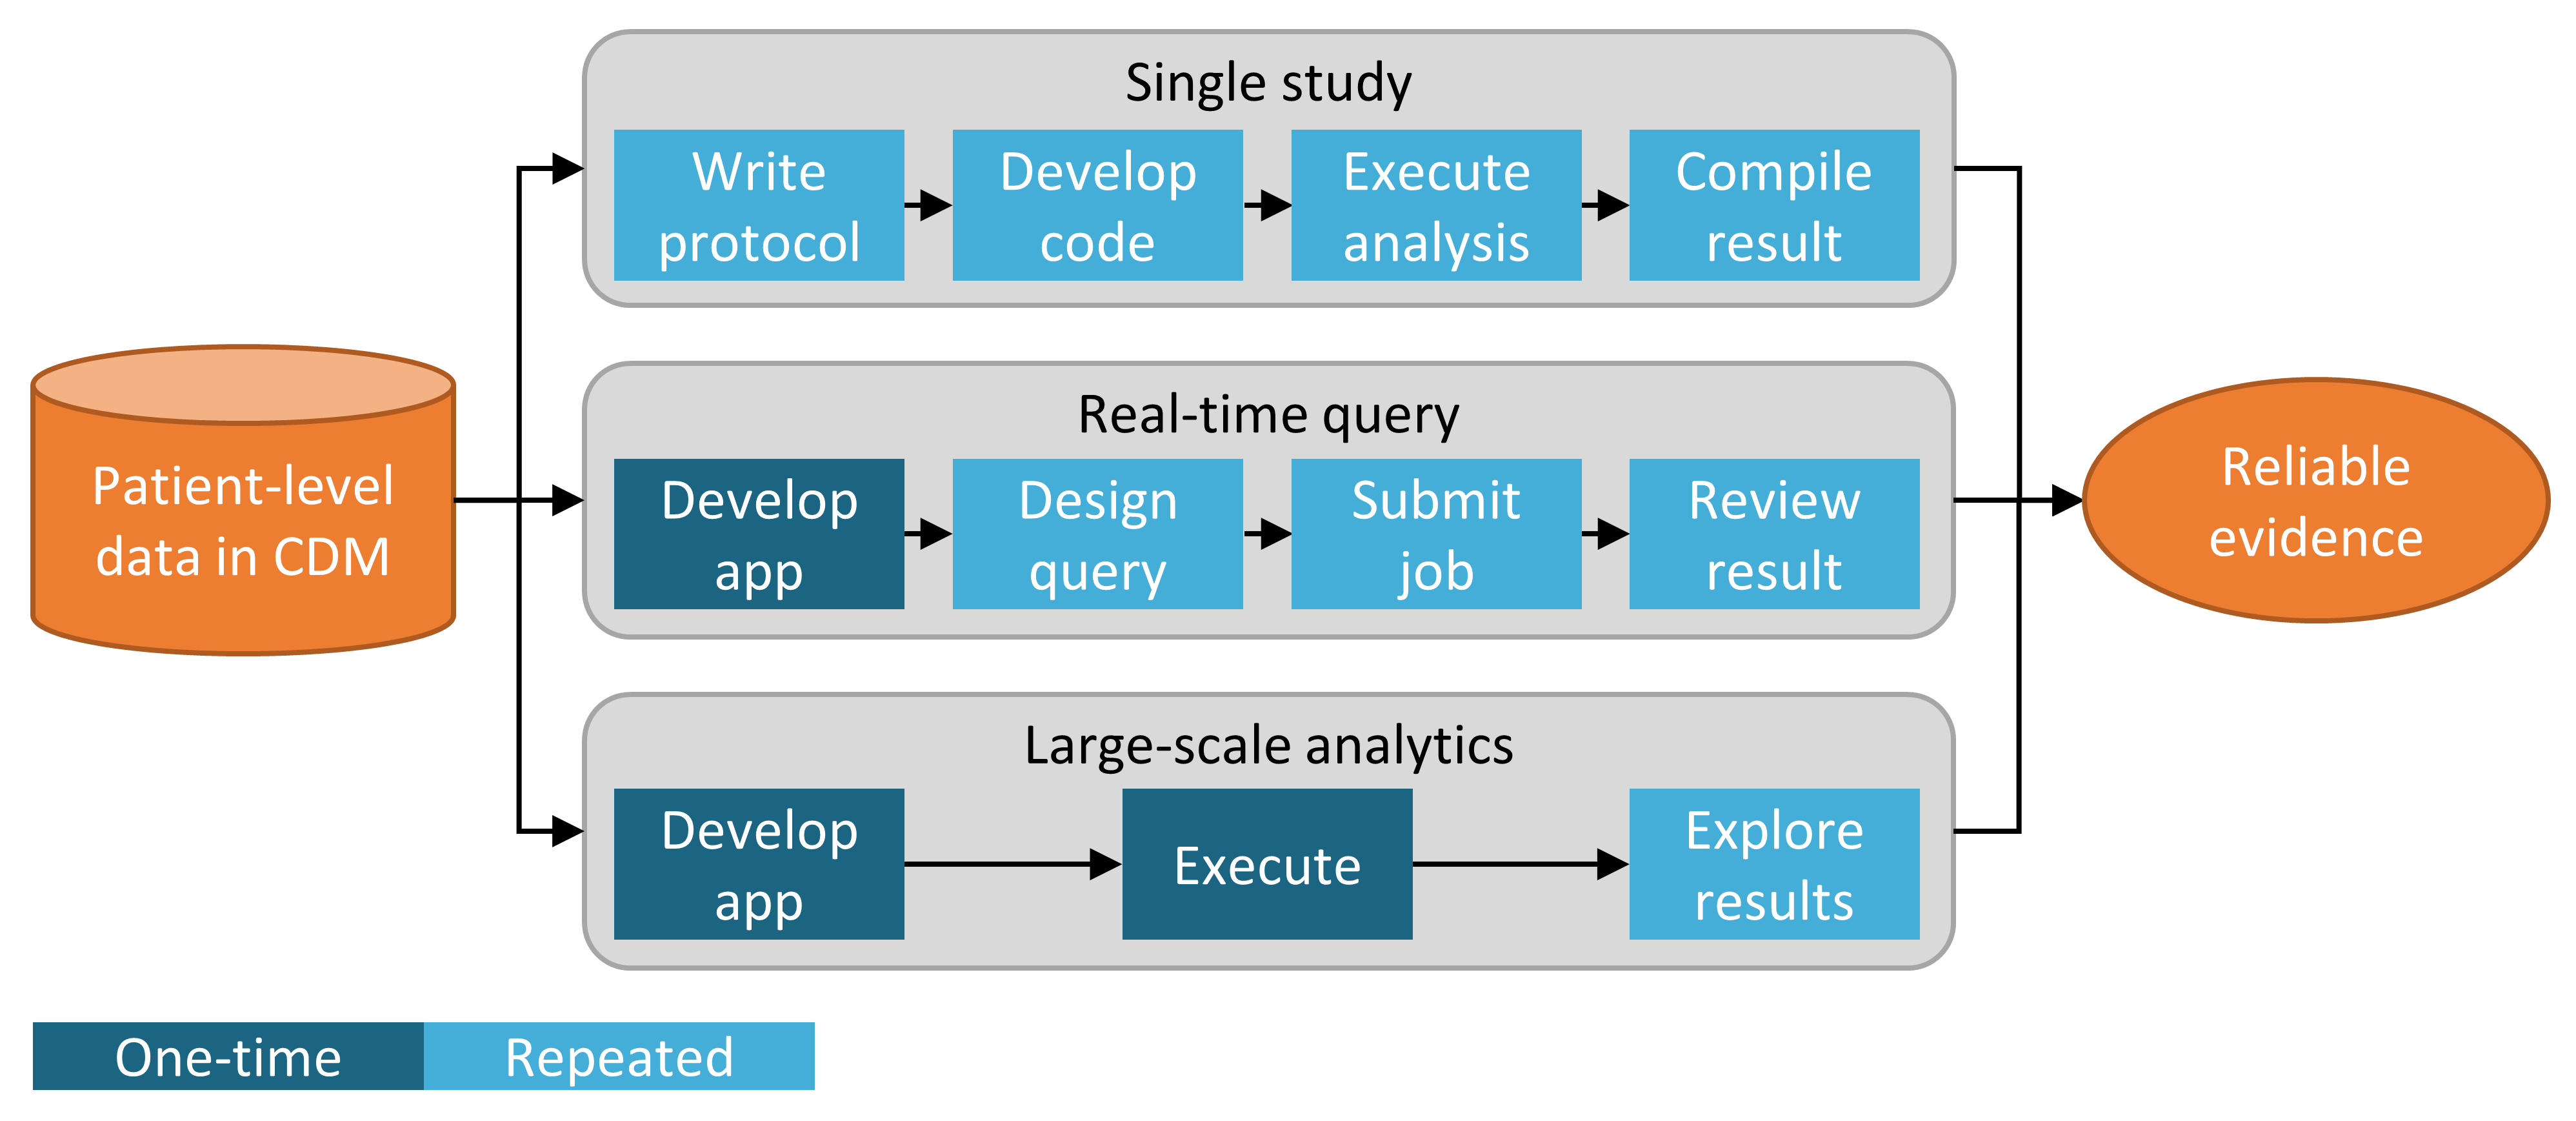
\includegraphics[width=0.9\linewidth]{images/OhdsiAnalyticsTools/strategies} 

}

\caption{(임상적) 질문에 대한 근거를 생성하기 위한 전략}\label{fig:strategies}
\end{figure}

첫 번째 전략은 모든 분석을 하나의 개별적인 연구로 본다. 분석은
프로토콜에 미리 지정되어야 하고, 코드로 구현되어야 하며, 데이터에 대해
실행되어야 하며, 그 후에 결과를 컴파일하고 해석할 수 있어야 한다. 모든
질문에 대해 모든 단계를 반복해야 한다. 그러한 분석의 예로는 phenytoin과
비교하여 levetiracetam과 관련된 혈관부종(angioedema)의 위험에 대한 OHDSI
연구가 있다. \citep{duke_2017} 이 연구에서, 프로토콜이 처음으로
작성되었고, OHDSI Methods Library를 이용한 분석 코드가 OHDSI 네트워크를
통해 개발되어 실행되었으며, 결과를 편집하여 저널 간행물에 배포하였다.

두 번째 전략은 사용자가 특정 종류의 질문에 실시간으로 또는 거의
실시간으로 답할 수 있는 애플리케이션을 개발한다. 애플리케이션이 개발되면
사용자는 애플리케이션과 상호 작용하여 쿼리를 정의하고 제출하고 결과를 볼
수 있다. 이 전략의 예로는 ATLAS의 코호트 정의 및 생성 도구가 있다. 이
도구는 사용자가 다양한 수준의 복잡한 코호트 정의를 내리고 원하는
데이터베이스에 대해 실행함으로써 얼마나 많은 환자가 다양한 포함 기준 및
제외 기준을 충족하는 지 알 수 있게 한다.

세 번째 전략은 비슷하게 한 클래스의 질문 a class of questions에 초점을
맞추지만, 일단 작동하기 시작하면 그 클래스에 속한 모든 의문점에 대해
광범위하고 철저하게 모든 근거를 남김없이 생성하려고 시도한다. 사용자는
다양한 인터페이스를 통해 필요에 따라 (미리 생성된) 근거를 탐색할 수
있다. 한 예로 우울증 치료의 영향에 대한 OHDSI 연구가 있다.
\citep{schuemie_2018b} 이 연구에서 모든 우울증 치료는 4개의 큰 관찰
데이터베이스에서 큰 규모의 임상결과 집합에 대해 비교된다. 광범위한 연구
진단과 함께 경험적으로 보정된 17,718개의 위험비 hazard ratio를 포함한
전체 결과는 대화형 웹 앱에서 이용할 수 있다. \footnote{\url{http://data.ohdsi.org/SystematicEvidence/}}

\section{ATLAS}\label{atlas}

ATLAS는 CDM 형식으로 표준화된 환자 수준 관찰 데이터에 대한 분석 설계와
실행을 도와주는 OHDSI 커뮤니티에서 개발한 무료 웹 기반 툴이다. ATLAS는
OHDSI WebAPI와 함께 웹 애플리케이션으로 배포되며 일반적으로 Apache
Tomcat에서 호스팅된다. 실시간 분석을 수행하려면 CDM에 있는 환자 수준
데이터에 액세스해야 하므로 일반적으로 조직의 방화벽 뒤에 설치된다.
그러나 공용 ATLAS\footnote{\url{http://www.ohdsi.org/web/atlas}}도
있으며, 이 ATLAS 인스턴스는 몇 개의 소규모 시뮬레이션 데이터 세트에만
액세스할 수 있지만, 여전히 테스트와 훈련을 포함한 여러 용도로 사용할 수
있다. ATLAS의 공개 인스턴스를 사용하여 효과 추정 또는 예측 연구를 완전히
정의하고, 연구를 실행하기 위한 R 코드를 자동으로 생성할 수도 있다. 이
코드는 ATLAS와 WebAPI를 설치할 필요 없이 사용 가능한 CDM이 있는 모든
환경에서 실행될 수 있다. \index{ATLAS}

\begin{figure}

{\centering 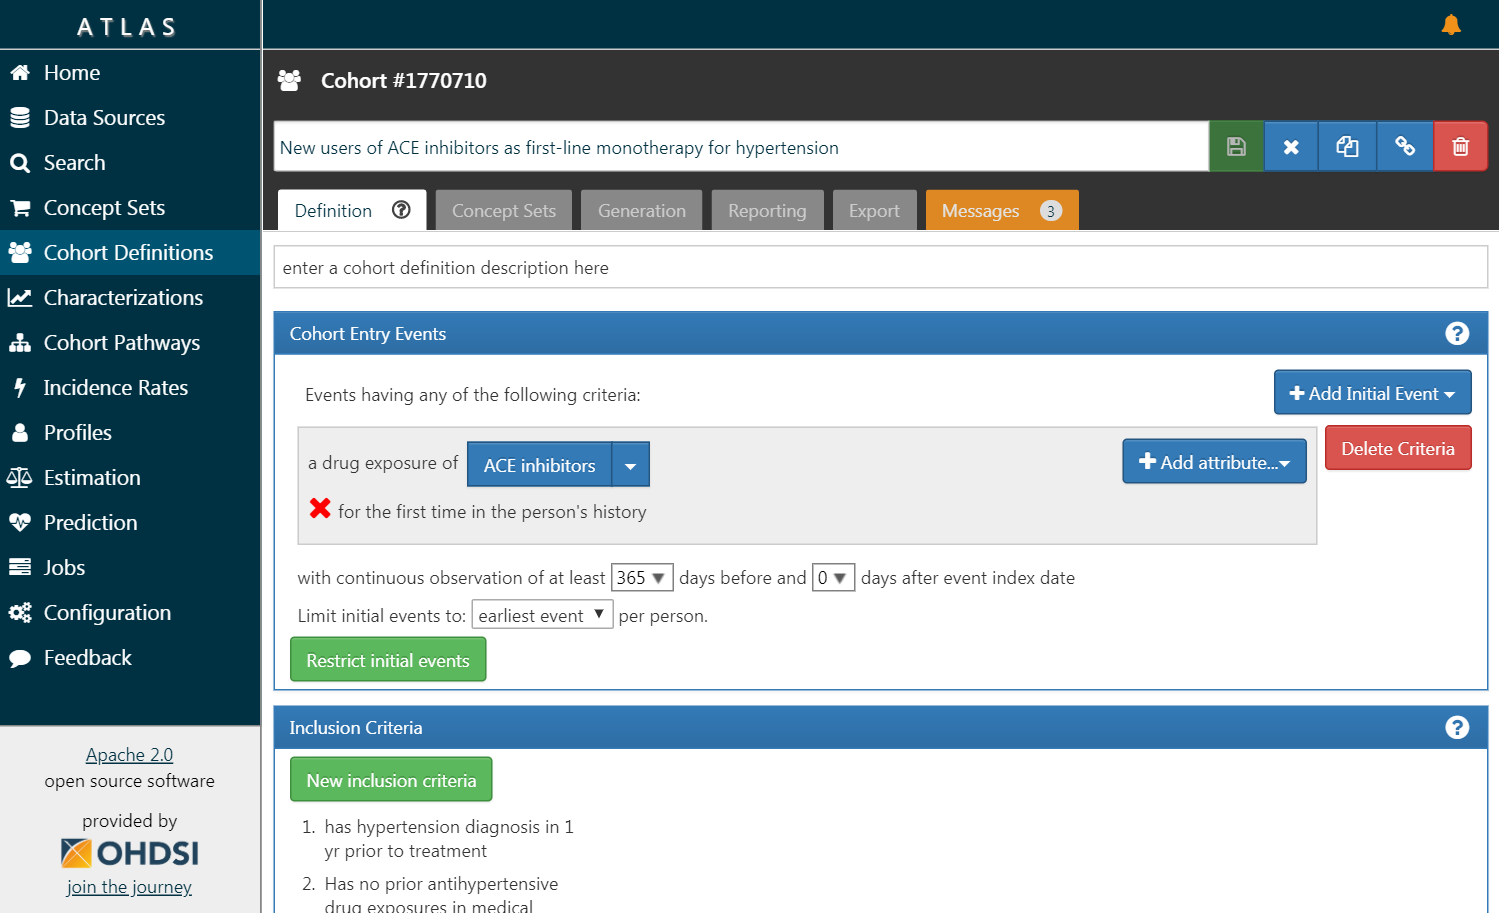
\includegraphics[width=1\linewidth]{images/OhdsiAnalyticsTools/atlas} 

}

\caption{ATLAS 사용자 인터페이스}\label{fig:atlas}
\end{figure}

ATLAS 스크린샷은 그림 \ref{fig:atlas}에 제공된다. 왼쪽에는 ATLAS에서
제공하는 다양한 기능을 보여주는 내비게이션 바가 있다:

\begin{description}
\tightlist
\item[Data Sources \index{ATLAS!Data Sources}
\index{Achilles|see {ATLAS!data sources}}]
데이터 원본(Data sources)은 Atlas 플랫폼 내에서 구성한 각 데이터 원본에
대해 기술적이고 표준화된 보고 기능을 제공한다. 이 기능은 대규모 분석
전략을 사용한다. 모든 기술통계량은 사전에 계산된 것이다. 데이터 출처는
\ref{Characterization}장에서 논한다.
\item[Vocabulary Search \index{ATLAS!vocabulary search}]
Atlas는 OMOP 표준용어집을 검색하고 탐색하여 그 어휘 안에 존재하는 개념과
데이터 소스에 대한 표준 분석에서 그 개념을 적용하는 방법을 이해할 수
있는 기능을 제공한다. 이 특성은 \ref{StandardizedVocabularies}장에서
논한다.
\item[Concept Sets \index{ATLAS!concept sets}]
개념 집합 concept set은 표준화된 분석에서 사용할 개념 집합을 식별하는 데
사용할 수 있는 논리 표현식의 집합을 만들 수 있게한다. 개념 집합은 단순한
코드나 값 리스트보다 더 정교하게 만들어 준다. 개념 집합은 사용자가 용어
계층에 관련 개념을 포함하거나 배제할 수 있도록 하는 논리적 지표와 함께
표준화된 어휘에서 나온 여러 개념으로 구성되어 있다. 용어를 검색하고,
개념 집합을 식별하며, 개념 집합을 해결하기 위해 사용할 논리를 명시하는
것은 분석 계획에서 흔히 접하는 모호한 의학 언어를 명확히 정의할 수 있게
하는 강력한 메커니즘을 제공한다. 이러한 개념 집합은 ATLAS 내에 저장한
다음 코호트 정의 또는 분석 규격의 일부로 분석 내내 사용할 수 있다.
\item[Cohort Definitions \index{ATLAS!cohort definitions}]
코호트 정의 Cohort Definition는 일정 기간 동안 하나 이상의 기준을
충족하는 일련의 사람들을 구성할 수 있게 하며, 이러한 코호트는 이후 모든
분석시 입력의 기초 basis of input가 된다. 이 특성은 \ref{Cohorts}장에서
논한다.
\item[Characterizations \index{ATLAS!cohort characterization}]
특성은 당신이 정의한 하나 이상의 코호트를 보고 그 환자군에 대한 특성을
요약할 수 있는 분석 기능이다. 이 기능은 실시간 쿼리 전략을 사용하며,
\ref{Characterization}장에서 논한다.
\item[Cohort Pathways \index{ATLAS!cohort pathways}]
코호트 경로(Cohort pathways)는 하나 이상의 인구집단 내에서 발생하는 임상
사건의 순서를 살펴볼 수 있는 분석 툴이다. 이 기능은 실시간 쿼리 전략을
사용하며, \ref{Characterization}장에서 논한다.
\item[Incidence Rates \index{ATLAS!incidence rates}]
발생률은 관심 대상 인구집단 내에서 임상결과의 발생률을 추정할 수 있는
도구다. 이 기능은 실시간 쿼리 전략을 사용하며,
\ref{Characterization}장에서 논한다.
\item[Profiles \index{ATLAS!profiles}]
프로파일은 개별 환자에 대해 종적 관찰 데이터를 탐색하여 특정 개인 내에서
일어나는 일을 요약할 수 있는 도구다. 이 기능은 실시간 쿼리 전략을
사용한다.
\item[Population Level Estimation
\index{ATLAS!population level estimation}]
추정은 비교 코호트 설계를 사용하여 인구 수준 효과 추정 연구를 정의할 수
있는 기능이며, 여기서 하나 이상의 대상 코호트와 비교 코호트 간의 비교를
통해 일련의 결과에 대해 탐색할 수 있다. 이 기능은 코딩이 필요하지
않으므로 실시간 쿼리 전략을 구현한다고 말할 수 있으며,
\ref{PopulationLevelEstimation}장에서 논의한다.
\item[Patient Level Prediction \index{ATLAS!patient level prediction}]
예측은 주어진 대상 노출 군 내에서 임상 결과를 예측할 수 있는 환자 수준
예측 분석을 수행하기 위해 기계 학습 알고리즘을 적용할 수 있는 기능이다.
이 기능은 코딩이 필요하지 않음으로 실시간 쿼리 전략을 구현한다고 할 수
있으며, \ref{PatientLevelPrediction}장에서 논한다.
\item[Jobs \index{ATLAS!jobs}]
WebAPI를 통해 실행 중인 프로세스의 상태를 탐색하려면 이 기능을 선택하라.
각각의 작업은 종종 코호트 특성 보고서를 생성하거나 코호트 특성화
보고서를 생성하는 것과 같은 장기 실행 과정이다.
\item[Configuration \index{ATLAS!configuration}]
소스 구성 섹션에 구성된 데이터 소스를 검토하려면 구성 메뉴 항목을
선택하라.
\item[Feedback \index{ATLAS!feedback}]
피드백 링크는 Atlas의 이슈 로그로 이동 시켜 새로운 이슈를 기록하거나
기존 이슈를 검색할 수 있도록 해준다. 새로운 기능이나 개선사항에 대한
아이디어가 있다면, 이것은 개발 커뮤니티에 대한 참고 사항이기도 하다.
\end{description}

\subsection{보안}

ATLAS와 WebAPI는 전체 플랫폼 내의 기능 또는 데이터 소스에 대한 액세스를
제어하기 위한 세분화된 보안 모델을 제공한다. 이 보안 시스템은 Apache
Shiro 라이브러리를 활용하여 구축된다. 보안 시스템에 대한 추가 정보는
온라인 WebAPI 보안 위키에서 찾을 수 있다. \footnote{\url{https://github.com/OHDSI/WebAPI/wiki/Security-Configuration}}
\index{ATLAS!security}

\subsection{설명서}

ATLAS에 대한 설명서는 ATLAS GitHub repository wiki.\footnote{\url{https://github.com/OHDSI/ATLAS/wiki}}
에 있다. 이 위키에는 온라인 비디오 튜토리얼에 대한 링크뿐만 아니라
다양한 애플리케이션 기능에 대한 정보가 포함되어 있다.
\index{ATLAS!documentation}

\subsection{설치 방법}\label{-}

ATLAS 설치는 OHDSI WebAPI와 함께 수행된다. 각 구성 요소의 설치 가이드는
ATLAS GitHub 저장소 설정 가이드\footnote{\url{https://github.com/OHDSI/Atlas/wiki/Atlas-Setup-Guide}}
및 WebAPI GitHub 저장소 설치 가이드\footnote{\url{https://github.com/OHDSI/WebAPI/wiki/WebAPI-Installation-Guide}}에서
찾아볼 수 있다. \index{ATLAS!installation}

\section{Methods Library}\label{methods-library}

The \href{https://ohdsi.github.io/MethodsLibrary/}{OHDSI Methods
Library}는 그림 \ref{fig:methodsLibrary}에 표시된 오픈 소스 R 패키지의
모음이다. \index{methods library}

\begin{figure}

{\centering 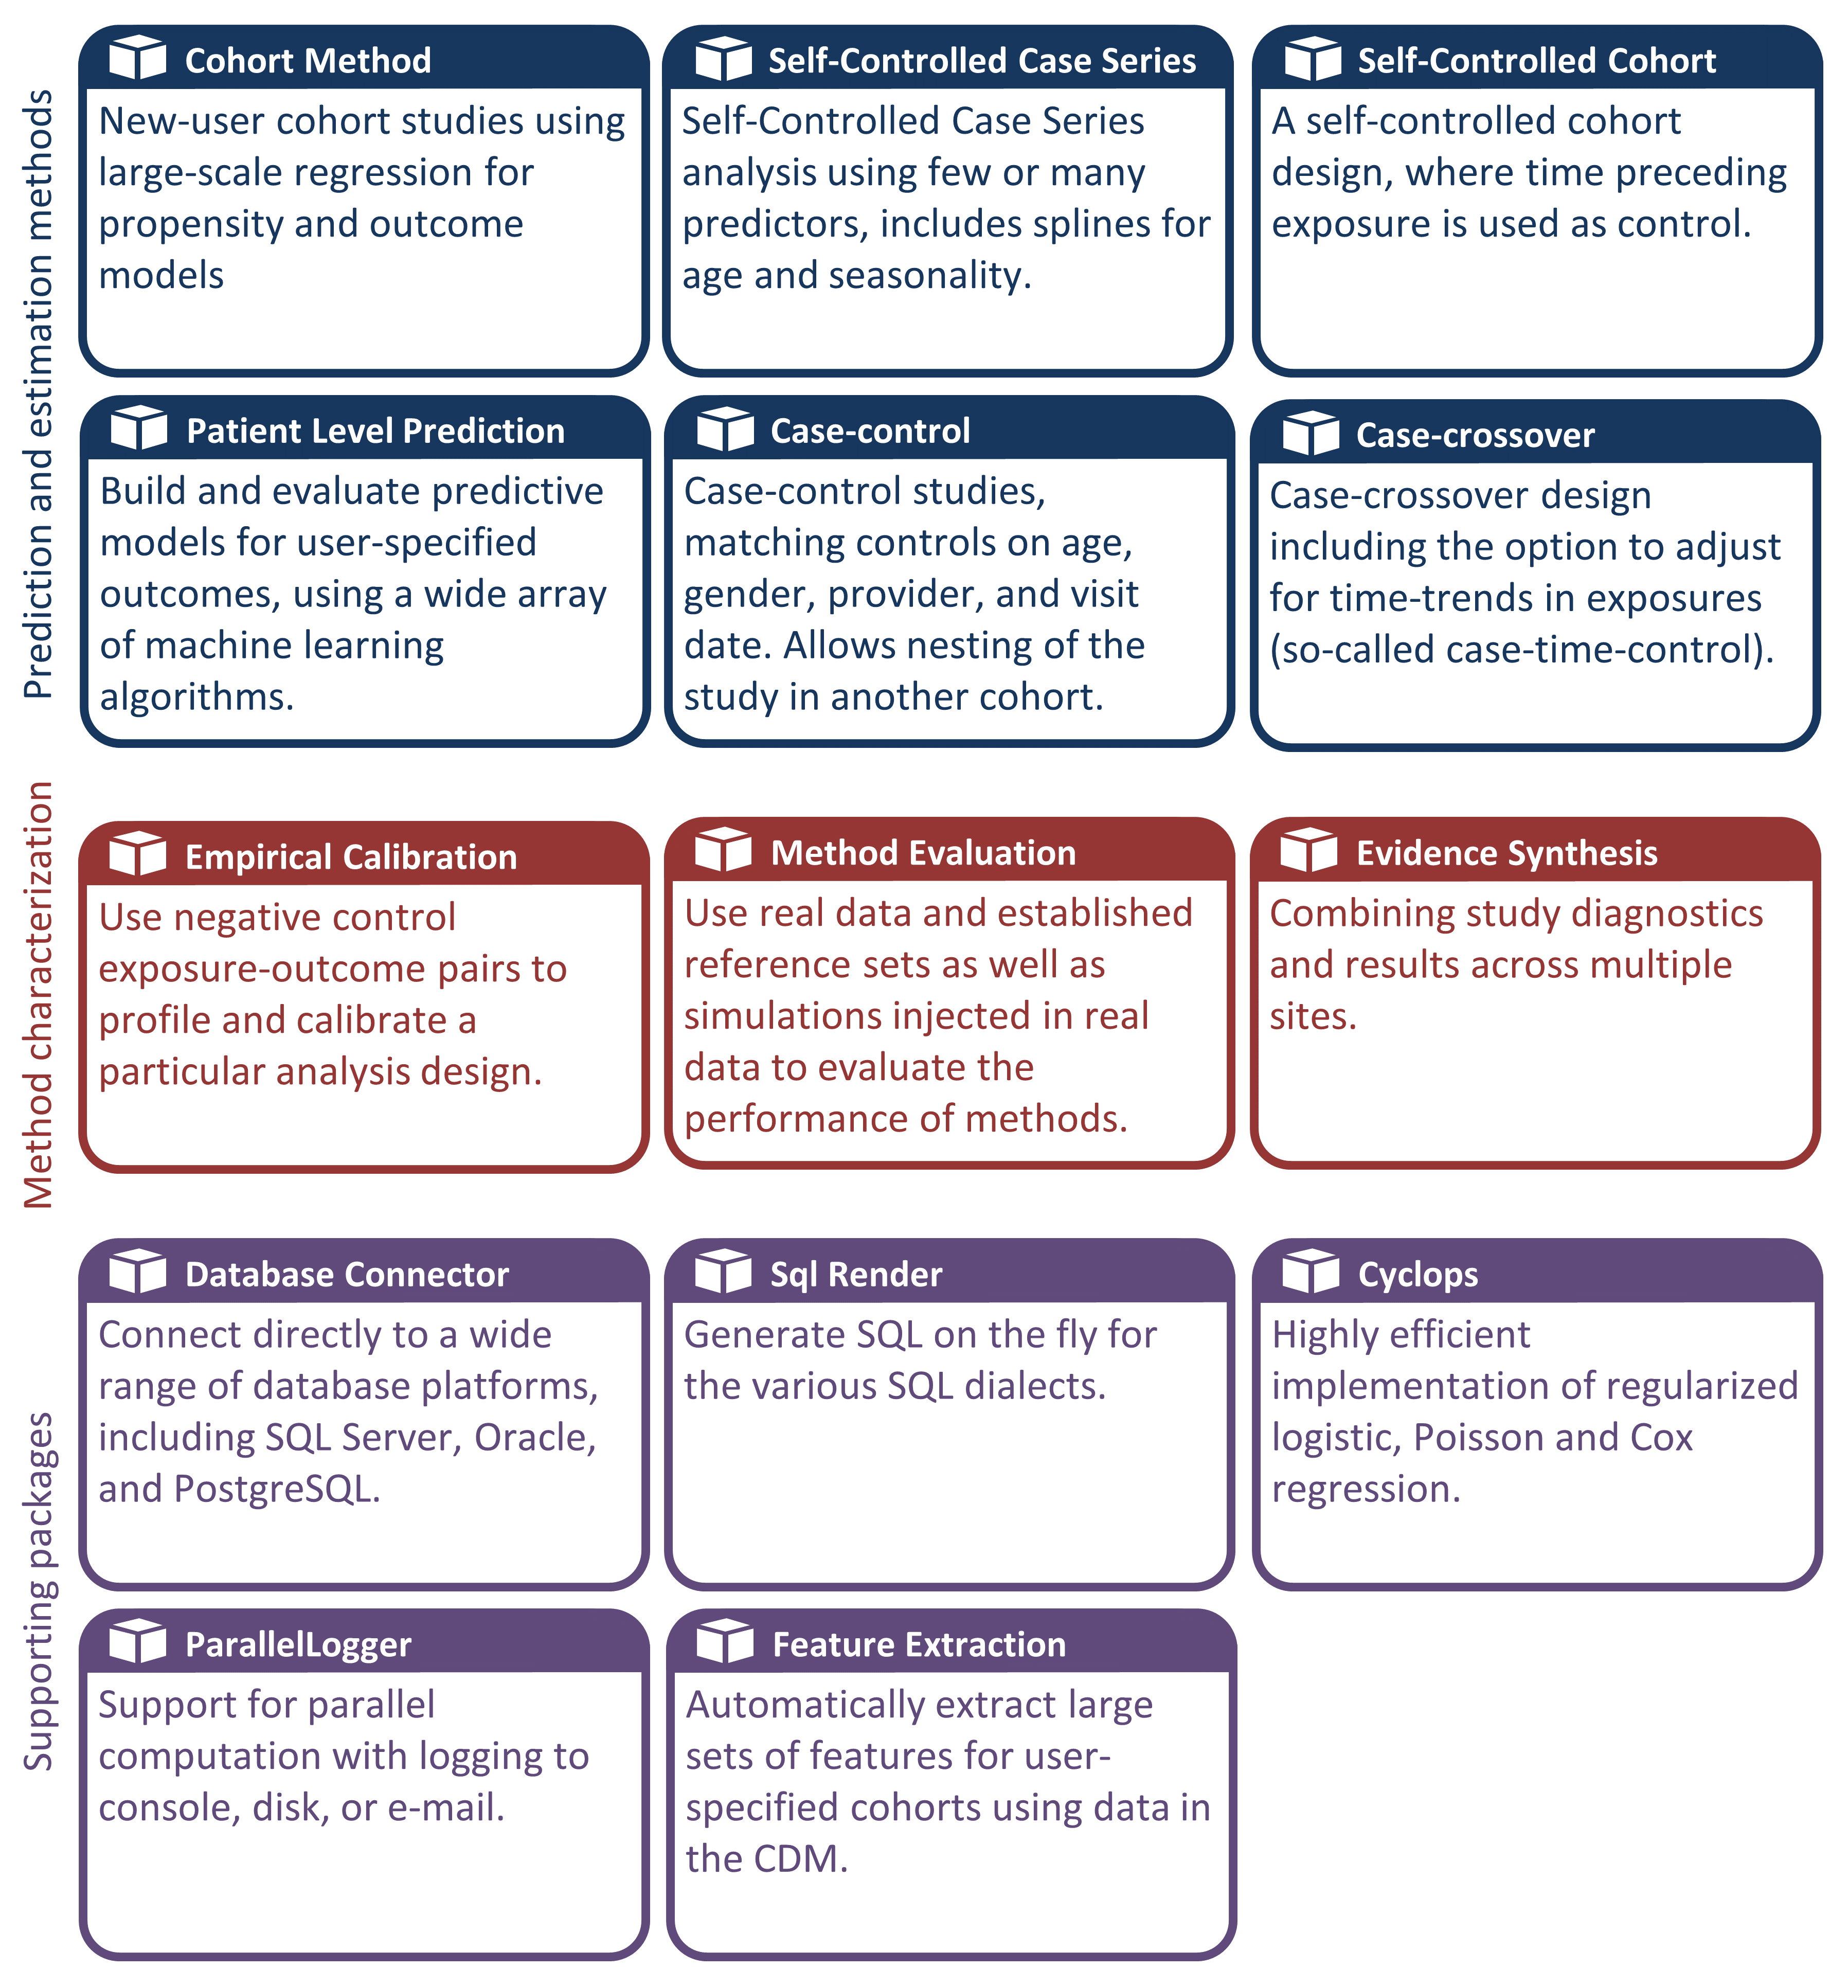
\includegraphics[width=1\linewidth]{images/OhdsiAnalyticsTools/methodsLibrary} 

}

\caption{The OHDSI Methods Library의 패키지}\label{fig:methodsLibrary}
\end{figure}

패키지는 완전한 관찰 연구를 수행하기 위해 함께 사용할 수 있는 R 기능을
제공하며, CDM의 데이터에서 시작하여 결과 추정치와 이를 뒷받침하는 통계,
수치 및 표를 제공한다. 패키지는 CDM의 관찰 데이터와 직접 상호작용하며,
단순히 \ref{SqlAndR}장에서 설명한 대로 완전한 사용자 정의 분석에 대한
플랫폼 간 호환성을 제공하는 데 사용하거나, 인구 특성화를 위한 고급
표준화 분석 (\ref{Characterization}장 참조), 인구 수준 효과 추정
(\ref{PopulationLevelEstimation}장 참조) 및 환자 수준 예측
(\ref{PatientLevelPrediction}장 참조) 을 제공할 수 있다. The Methods
Library는 (이전 또는 진행 중인 연구에서 학습한) 투명성, 재현성, 그뿐만
아니라 ``특정 맥락에서 methods의 작동 특성(operating characteristics)
측정'' 및 이어지는 ``methods로부터 생성된 측정치의 경험적 교정(empirical
calibration)''과 같은 관찰 데이터 및 관찰 연구 설계의 사용을 위한 모범
사례를 지원한다.

Method Library는 이미 발표된 많은 임상 연구
\citep{boland_2017, duke_2017, ramcharran_2017, weinstein_2017, wang_2017, ryan_2017, ryan_2018, vashisht_2018, yuan_2018, johnston_2019}와
방법론 연구에 사용되어 왔다.
\citep{schuemie_2014, schuemie_2016, reps2018, tian_2018, schuemie_2018, schuemie_2018b, reps_2019}
The Methods Library에서 방법론 구현의 타당성은
\ref{SoftwareValidity}장에 설명되어 있다.

\subsection{대규모 분석 지원}\label{--}

모든 패키지에 통합된 한 가지 주요 특징은 많은 분석을 효율적으로 실행할
수 있는 능력이다. 예를 들어 인구 수준 추정을 수행할 때 CohortMethod
패키지는 다양한 분석 설정을 사용하여 많은 노출(exposure) 및
결과(outcome)에 대한 효과 크기 추정치(effect-size estimates)를 계산할 수
있도록 하며, 패키지는 필요한 모든 중간 및 최종 데이터 세트를 계산하는
최적의 방법을 자동으로 선택한다. ``공변량 추출(extraction of
covariates)''이나 하나의 대상군-비교군 쌍(target-comparator pair)과
복수의 결과에 사용되는 ``성향 모델 맞춤(fitting a propensity model)''과
같이 재사용할 수 있는 단계는 한 번만 실행된다. 가능한 경우 계산 자원의
사용을 극대화하기 위해 연산은 병렬처리 될 것이다.

이러한 효율적 계산은 대규모 분석을 가능하게 하여 한꺼번에 많은 질문에
답할 수 있으며, 또한 제어 가설(예를 들어, 음성대조군(negative
controls)을 포함해 방법론의 작동 특성(operating characteristics)을
측정하고 \ref{MethodValidity}장에 기술된 경험적 교정(empirical
calibration)을 수행하는 데 필수적이다. \index{control hypotheses}

\subsection{빅데이터 지원}\label{BigDataSupport}

The Methods Library는 또한 매우 큰 데이터베이스에 대해 실행하고 대량의
데이터를 포함하는 계산을 수행할 수 있도록 설계되었다. 이는 다음과 같은
세 가지 방법으로 달성되었다:

\begin{enumerate}
\def\labelenumi{\arabic{enumi}.}
\tightlist
\item
  대부분의 데이터 조작은 데이터베이스 서버에서 수행된다. 분석은
  일반적으로 데이터베이스에 있는 전체 데이터의 극히 일부만을 필요로 하며
  Methods Library는 SqlRender 및 DatabaseConnector 패키지를 통해
  서버에서 고급 작업을 수행하여 관련 데이터를 사전 처리하고 추출할 수
  있도록 한다.
\item
  대용량 로컬 데이터 객체는 메모리 효율적인 방식으로 저장된다. 로컬
  시스템으로 다운로드되는 데이터의 경우 Method Library는
  \href{https://cran.r-project.org/web/packages/ff}{ff} 패키지를
  사용하여 대용량 데이터 객체를 저장하고 작업한다. 이것은 우리가
  메모리를 직접적으로 사용하는 것보다 훨씬 더 큰 데이터로 작업할 수 있게
  해준다.
\item
  필요한 곳에 고성능 컴퓨팅을 적용한다. 예를 들어,
  \href{https://ohdsi.github.io/Cyclops/}{Cyclops} 패키지는 대량의
  변수와 관측치로 인해 다른 방법으로는 할 수 없는 대규모 회귀를 수행할
  수 있는 매우 효율적인 회귀 엔진을 구현했으며 Methods Library 전체에서
  이 엔진을 사용할 수 있다.
\end{enumerate}

\subsection{문서화}

R은 패키지를 문서화하는 표준화된 방법을 제공한다. 각 패키지에는 패키지에
포함된 모든 기능과 데이터 세트를 문서화하는 \emph{패키지 설명서}가 있다.
모든 패키지 매뉴얼은 the Methods Library 웹 사이트\footnote{\url{https://ohdsi.github.io/MethodsLibrary}}를
통해 패키지 GitHub 온라인 저장소를 통해 사용할 수 있으며 CRAN을 통해
사용할 수 있는 패키지의 경우는 CRAN에서 찾을 수 있다. 또한, R 내에서
물음표를 사용하여 패키지 설명서를 참조할 수 있다. 예를 들어
DatabaseConnector 패키지를 로드한 후 \texttt{?connect} 명령을 입력하면
``연결(connect)'' 기능에 대한 문서가 나타난다.

패키지 설명서 외에도 많은 패키지가 \emph{vignette}를 제공한다.
Vignettes는 특정 작업을 수행하기 위해 어떻게 패키지를 사용할 수 있는지
설명하는 긴 형식의 문서다. 예를 들어, 하나의 vignette\footnote{\url{https://ohdsi.github.io/CohortMethod/articles/MultipleAnalyses.html}}은
CohortMethod 패키지를 사용하여 여러 가지 분석을 효율적으로 수행하는
방법을 설명한다. 또한 Vignettes는 Methods Library 웹 사이트, 패키지
GitHub 저장소를 통해 찾을 수 있으며, CRAN을 통해 이용할 수 있는 패키지의
경우 CRAN에서 찾을 수 있다. Vignettes는 the Methods Library 웹 사이트를
통해 패키지 GitHub 온라인 저장소를 통해 사용할 수 있으며 CRAN을 통해
사용할 수 있는 패키지의 경우 CRAN에서 찾을 수 있다. \index{vignette}

\subsection{시스템 요구 사항}\label{--}

시스템 요구 사항을 논의할 때 두 가지 컴퓨팅 환경을 고려해야 한다:
데이터베이스 서버 및 분석 워크스테이션 \index{system requirements}

데이터베이스 서버는 관찰 의료 데이터를 CDM 형식으로 보관해야 한다.
Method Library는 전통적인 데이터베이스 시스템 (PostgreSQL, Microsoft SQL
Server, 그리고 Oracle), 병렬 데이터 웨어하우스 (Microsoft APS, IBM
Netezza, 그리고 Amazon RedShift) 및 빅데이터 플랫폼 (Impala를 통한
Hadoop, 그리고 Google BigQuery) 을 포함한 광범위한 데이터베이스 관리
시스템을 지원한다.

분석 워크스테이션은 Methods Library가 설치되어 실행되는 곳이다. 이것은
누군가의 랩톱과 같은 로컬 시스템이나 RStudio Server를 실행하는 원격
서버일 수 있다. 모든 경우에, R은 RStudio와 함께 설치되어야 한다. Methods
Library는 또한 Java가 설치되어야 한다. 분석 워크스테이션은 데이터베이스
서버에 연결할 수 있어야 하며, 특히 이들 사이의 방화벽은 데이터베이스
서버 접근스 포트를 워크스테이션에 개방해야 한다. 일부 분석은 계산
집약적일 수 있으므로 여러 개의 처리 코어와 충분한 메모리를 갖는 것이
분석 속도를 높이는 데 도움이 될 수 있다. 적어도 4개의 코어와 16GB의
메모리를 가질 것을 추천한다.

\subsection{설치 방법}\label{installR}

다음은 OHDSI R 패키지를 실행하는 데 필요한 환경을 설치하는 단계다. 다음
네 가지를 설치해야 한다: \index{R!installation}

\begin{enumerate}
\def\labelenumi{\arabic{enumi}.}
\tightlist
\item
  \textbf{R}은 통계 컴퓨팅 환경이다. 그것은 주로 명령어 인터페이스인
  기본 사용자 인터페이스와 함께 제공된다.
\item
  \textbf{RTools}는 Windows에서 소스로부터 R 패키지를 만드는 데 필요한
  프로그램들의 모음이다.
\item
  \textbf{RStudio}는 R을 사용하기 쉽게 하는 통합 개발 환경 (IDE,
  Integrated Development Environment) 이다. 여기에는 코드 편집기, 디버깅
  및 시각화 도구가 포함되어 있다. 사용하기 편한 유저인터페이스를
  원한다면 사용하기를 권한다.
\item
  \textbf{Java}는 OHDSI R 패키지의 일부 구성 요소 (예를 들어,
  데이터베이스에 연결하는 데 필요한 구성 요소) 를 실행하는 데 필요한
  컴퓨팅 환경이다.
\end{enumerate}

아래에서는 Windows 환경에 이러한 각 항목을 설치하는 방법에 대해
설명한다.

\BeginKnitrBlock{rmdimportant}
윈도우즈에서 R과 Java는 32-bit 및 64-bit 아키텍처를 모두 제공한다. 두
아키텍처에 R을 설치하는 경우, \textbf{반드시} 두 아키텍처에 모두 Java를
설치해야 한다. R은 64-bit 버전만 설치하는 것을 추천한다.
\EndKnitrBlock{rmdimportant}

\subsubsection*{R 설치하기}\label{r-}
\addcontentsline{toc}{subsubsection}{R 설치하기}

\begin{enumerate}
\def\labelenumi{\arabic{enumi}.}
\tightlist
\item
  \url{https://cran.r-project.org/}으로 이동하여, ``Download R for
  Windows''를 클릭 후 ``base''를 클릭한 다음 그림 \ref{fig:downloadR}에
  표시된 다운로드 링크를 클릭하라.
\end{enumerate}

\begin{figure}

{\centering 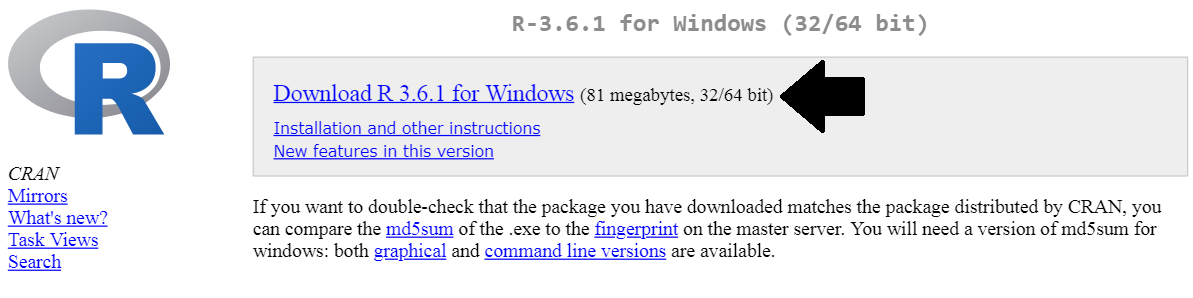
\includegraphics[width=1\linewidth]{images/OhdsiAnalyticsTools/downloadR} 

}

\caption{CRAN으로부터 R 다운로드}\label{fig:downloadR}
\end{figure}

\begin{enumerate}
\def\labelenumi{\arabic{enumi}.}
\setcounter{enumi}{1}
\tightlist
\item
  다운로드가 완료된 후 설치 프로그램을 실행하라. 다음 두 가지 예외를
  제외하고 모든 곳에서 기본 옵션을 사용하라. 첫째, 프로그램 파일 폴더에
  설치하지 않는 것이 좋다. 대신 R을 그림 \ref{fig:rDestination}과 같이 C
  드라이브의 하위 폴더로 만들라. 둘째, R과 Java 간의 아키텍처 차이로
  인한 문제를 방지하려면 그림 \ref{fig:no32Bits}과 같이 32-bit
  아키텍처를 비활성화하라.
\end{enumerate}

\begin{figure}

{\centering 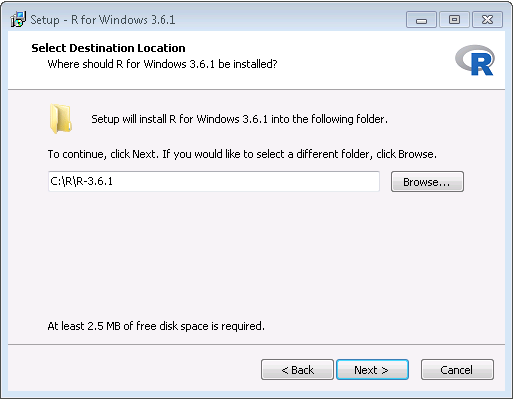
\includegraphics[width=0.8\linewidth]{images/OhdsiAnalyticsTools/rDestination} 

}

\caption{R의 대상 폴더 설정하기.}\label{fig:rDestination}
\end{figure}

\begin{figure}

{\centering 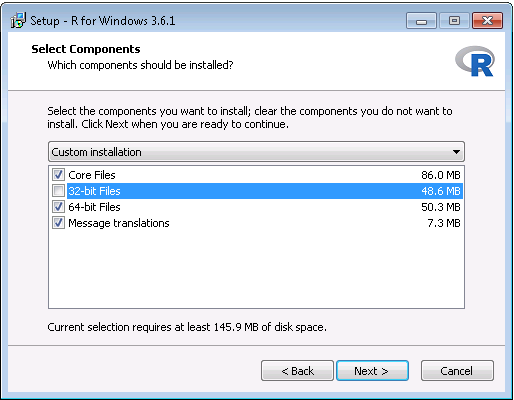
\includegraphics[width=0.8\linewidth]{images/OhdsiAnalyticsTools/no32Bits} 

}

\caption{32-bit 버전의 R을 사용하지 않도록 설정하기.}\label{fig:no32Bits}
\end{figure}

완료되면 시작 메뉴에서 R을 선택할 수 있어야 한다.

\subsubsection*{RTools 설치하기}\label{rtools-}
\addcontentsline{toc}{subsubsection}{RTools 설치하기}

\begin{enumerate}
\def\labelenumi{\arabic{enumi}.}
\item
  \url{https://cran.r-project.org/},으로 이동하여 ``Windows용 R
  다운로드''를 클릭한 다음 ``Rtools''를 클릭하고 다운로드할 최신 버전의
  RTools를 선택하라.
\item
  다운로드가 완료된 후 설치 프로그램을 실행하라. 어디에서나 기본 옵션을
  선택하라.
\end{enumerate}

\subsubsection*{RStudio 설치하기}\label{rstudio-}
\addcontentsline{toc}{subsubsection}{RStudio 설치하기}

\begin{enumerate}
\def\labelenumi{\arabic{enumi}.}
\tightlist
\item
  \url{https://www.rstudio.com/}으로 이동하여, ``Download RStudio''을
  선택 (또는 ``RStudio''에서 ``Download'' 버튼을 선택) 하고, 무료 버전을
  선택한 후, 그림 \ref{fig:downloadRStudio}과 같이 Windows용 설치
  프로그램을 다운로드하라.
\end{enumerate}

\begin{figure}

{\centering 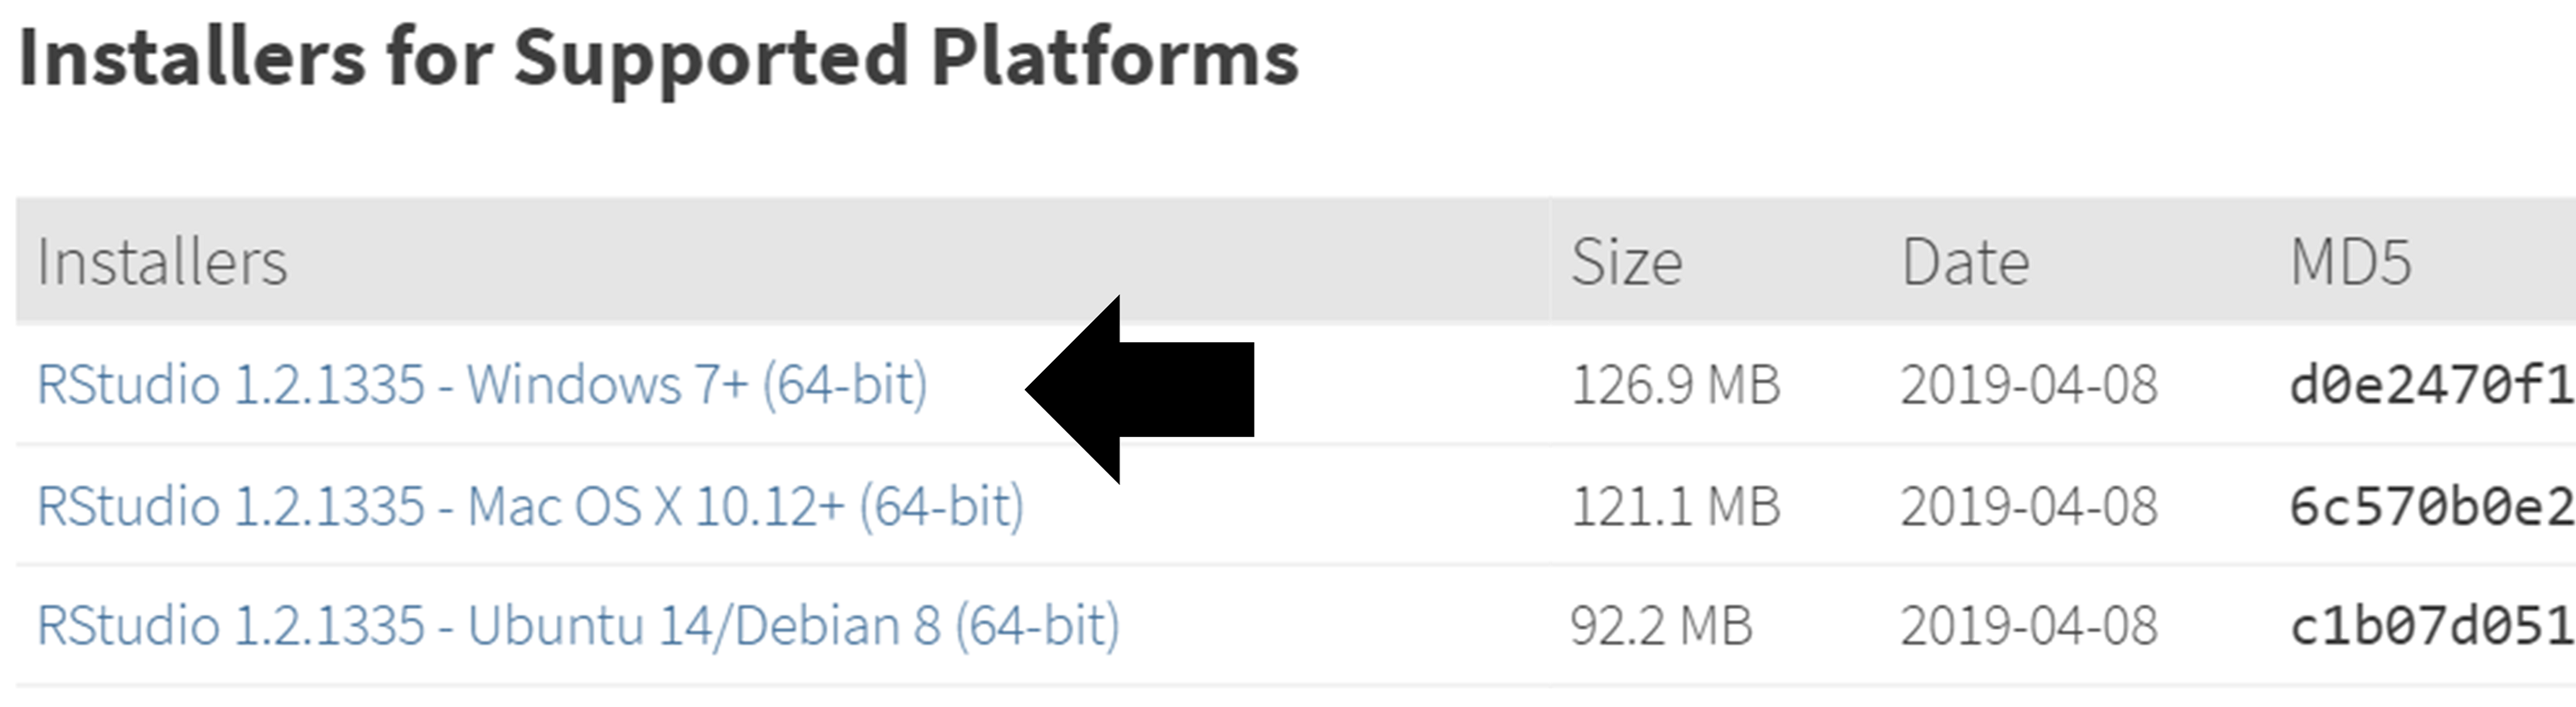
\includegraphics[width=1\linewidth]{images/OhdsiAnalyticsTools/downloadRStudio} 

}

\caption{RStudio 다운로드}\label{fig:downloadRStudio}
\end{figure}

\begin{enumerate}
\def\labelenumi{\arabic{enumi}.}
\setcounter{enumi}{1}
\tightlist
\item
  다운로드한 후, 설치 관리자를 시작하고, 모든 곳에서 기본 옵션을
  선택하라.
\end{enumerate}

\subsubsection*{Java 설치하기}\label{java-}
\addcontentsline{toc}{subsubsection}{Java 설치하기}

\begin{enumerate}
\def\labelenumi{\arabic{enumi}.}
\tightlist
\item
  \url{https://java.com/en/download/manual.jsp}으로 이동하여, 그림
  \ref{fig:downloadJava}와 같이 Windows 64-bit installer를 선택하라.
  32-bit 버전의 R을 설치한 경우 \emph{반드시} 다른 32-bit 버전의 Java도
  설치해야 한다.
\end{enumerate}

\begin{figure}

{\centering 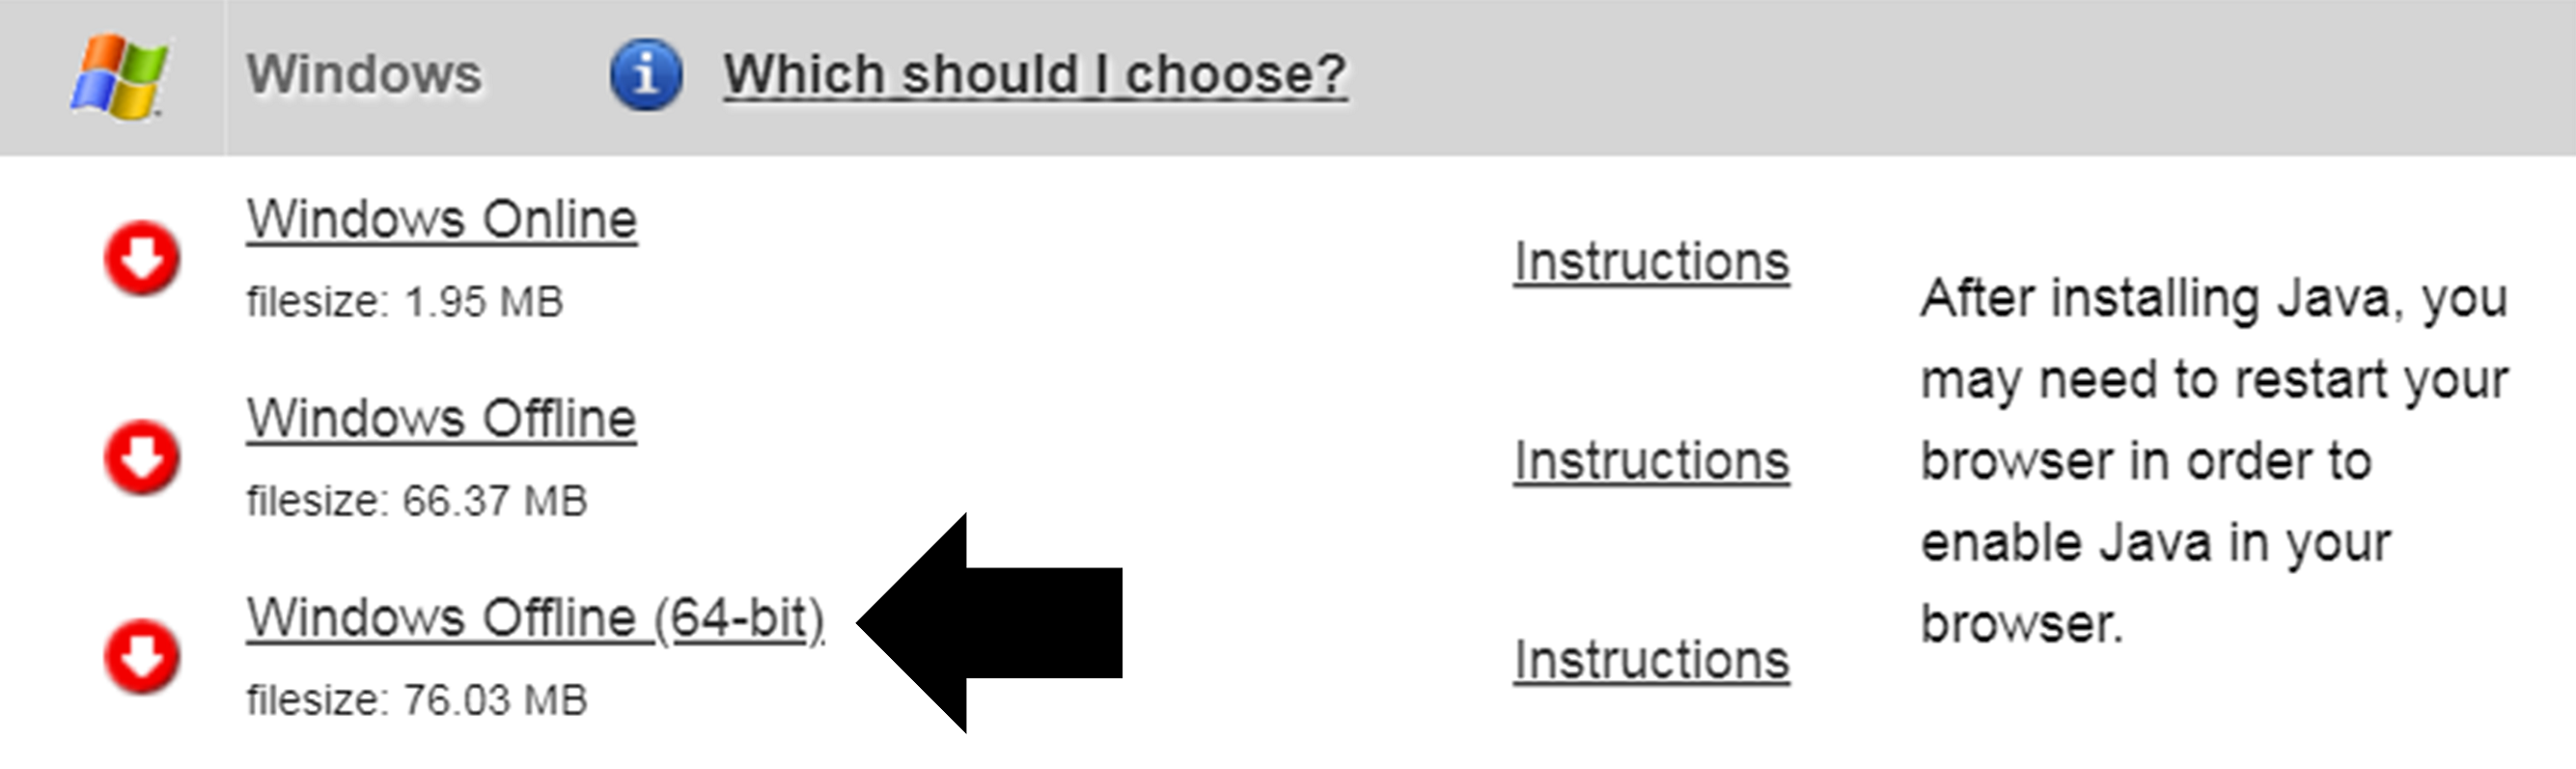
\includegraphics[width=1\linewidth]{images/OhdsiAnalyticsTools/downloadJava} 

}

\caption{Java 다운로드}\label{fig:downloadJava}
\end{figure}

\begin{enumerate}
\def\labelenumi{\arabic{enumi}.}
\setcounter{enumi}{1}
\tightlist
\item
  다운로드한 후 설치 프로그램을 실행하라.
\end{enumerate}

\subsubsection*{설치 검수하기}\label{-}
\addcontentsline{toc}{subsubsection}{설치 검수하기}

이제 시작할 준비를 해야 하지만, 그 전에 확실히 해야 한다. RStudio를
시작하고 및 아래의 내용을 입력하자.

\begin{Shaded}
\begin{Highlighting}[]
\KeywordTok{install.packages}\NormalTok{(}\StringTok{"SqlRender"}\NormalTok{)}
\KeywordTok{library}\NormalTok{(SqlRender)}
\KeywordTok{translate}\NormalTok{(}\StringTok{"SELECT TOP 10 * FROM person;"}\NormalTok{, }\StringTok{"postgresql"}\NormalTok{)}
\end{Highlighting}
\end{Shaded}

\begin{verbatim}
## [1] "SELECT  * FROM person LIMIT 10;"
\end{verbatim}

이 기능은 Java를 사용하기 때문에, 만약 모든 것이 잘 된다면, R과 Java가
모두 올바르게 설치되었다는 것을 알 수 있다!

또 다른 테스트는 소스 패키지를 제대로 구축할 수 있는지 확인하는 것이다.
다음 R 코드를 실행하여 OHDSI GitHub 저장소에서 \texttt{CohortMethod}
패키지를 설치하라:

\begin{Shaded}
\begin{Highlighting}[]
\KeywordTok{install.packages}\NormalTok{(}\StringTok{"drat"}\NormalTok{)}
\NormalTok{drat}\OperatorTok{::}\KeywordTok{addRepo}\NormalTok{(}\StringTok{"OHDSI"}\NormalTok{)}
\KeywordTok{install.packages}\NormalTok{(}\StringTok{"CohortMethod"}\NormalTok{)}
\end{Highlighting}
\end{Shaded}

\section{배치 전략}\label{-}

ATLAS 및 Method Library를 포함한 전체 OHDSI 도구 스택을 조직에 배치하는
것은 어려운 작업이다. 의존성 높은 구성 요소들을 많이 고려해야 하고,
설정해야 할 환경이 많다. 이 때문에 두 이니셔티브 (Broadsea와 AWS(Amazon
Web Services)) 는 일부 가상화 형태를 이용해 전체 스택을 하나의 패키지로
설치할 수 있는 통합 배치 전략을 개발했다. \index{tools deployment}

\subsection{Broadsea}\label{broadsea}

Broadsea\footnote{\url{https://github.com/OHDSI/Broadsea}}는 Docker
컨테이너 기술을 사용한다. \footnote{\url{https://www.docker.com/}} OHDSI
도구는 라이브러리간 의존성과 함께 Docker Image라는 단일 휴대용 이진
파일로 패키징된다. 그러면 이 이미지는 Docker 엔진 서비스에서 실행되고,
모든 소프트웨어가 설치되어 실행 준비가 된 가상 시스템(virtual machine)을
생성할 수 있다. Docker 엔진은 마이크로소프트 윈도우, 맥OS, 리눅스를
포함한 대부분의 운영 체제에 사용할 수 있다. Broadsea Docker 이미지에는
Methods Library와 ATLAS를 포함한 주요 OHDSI 도구가 포함되어 있다.
\index{tools deployment!Broadsea}

\subsection{Amazon AWS}\label{amazon-aws}

Amazon은 버튼 클릭 한 번으로 OHDSI환경을 AWS 클라우드 컴퓨팅 환경에서
바로 인스턴스화할 수 있는 두 가지 환경, 즉 OHDSI-in-a-Box\footnote{\url{https://github.com/OHDSI/OHDSI-in-a-Box}}와
OHDSIonAWS.\footnote{\url{https://github.com/OHDSI/OHDSIonAWS}}을
준비했다. \index{tools deployment!Amazon AWS}

OHDSI-in-a-Box는 특별히 학습 환경으로 만들어졌으며, OHDSI 커뮤니티에서
제공하는 대부분의 튜토리얼에 사용된다. 그것은 많은 OHDSI 도구, 샘플
데이터 세트, RStudio 및 기타 지원 소프트웨어를 저렴한 단일 윈도우즈 가상
머신에 포함했다. PostgreSQL 데이터베이스는 CDM을 저장하고 ATLAS의 중간
결과를 저장하는 데 사용된다. OMOP CDM 데이터 매핑과 ETL 툴도
OHDSI-in-a-Box에 포함되어 있다. OHDSI-in-a-Box 아키텍처는 그림
\ref{fig:ohdsiinaboxDiagram}에 나타나 있다.

\begin{figure}

{\centering 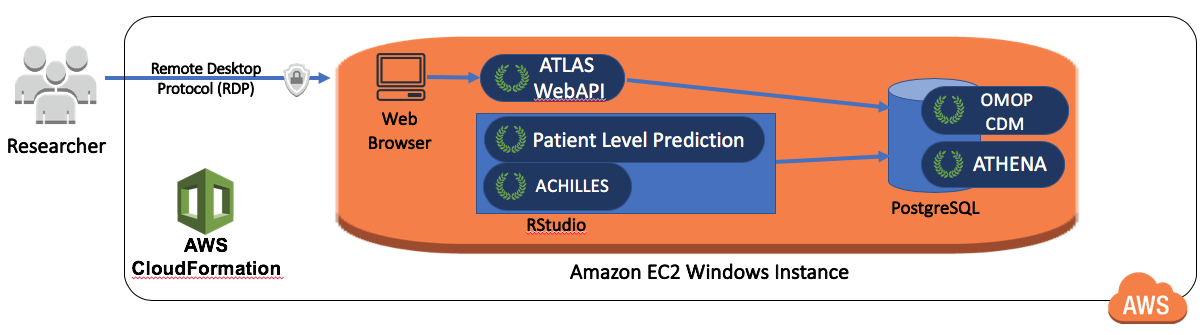
\includegraphics[width=1\linewidth]{images/OhdsiAnalyticsTools/OHDSI-in-a-BoxDiagram} 

}

\caption{OHDSI-in-a-Box용 Amazon Web Services 아키텍처}\label{fig:ohdsiinaboxDiagram}
\end{figure}

OHDSIonAWS는 기관이 그들의 데이터 분석을 수행하는 데 사용할 수 있는
엔터프라이즈급, 다중 사용자, 확장 가능하고 내결함성 OHDSI 환경을 위한
참조 아키텍처이다. 여기에는 몇 가지 샘플 데이터 세트가 포함되어 있으며
기관의 실제 의료 데이터를 자동으로 적재할 수도 있다. 데이터는 OHDSI
도구에 의해 지원되는 Amazon Redshift 데이터베이스 플랫폼에 배치된다.
ATLAS의 중간 결과는 PostgreSQL 데이터베이스에 저장된다. 프런트 엔드에서
사용자는 웹 인터페이스(leveraging RStudio Server)를 통해 ATLAS와
RStudio에 접근할 수 있다. RStudio에는 OHDSI Methods Library가 이미
설치되어 있으며, 데이터베이스에 연결하는 데 사용할 수 있다. OHDSIonAWS를
배포하는 자동화 도구는 오픈 소스로서 기관의 관리 툴과 모범 사례를
포함하도록 사용자 정의할 수 있다. OHDSIonAWS에 대한 아키텍처는 그림
\ref{fig:ohdsionawsDiagram}에 설명되어 있다.

\begin{figure}

{\centering 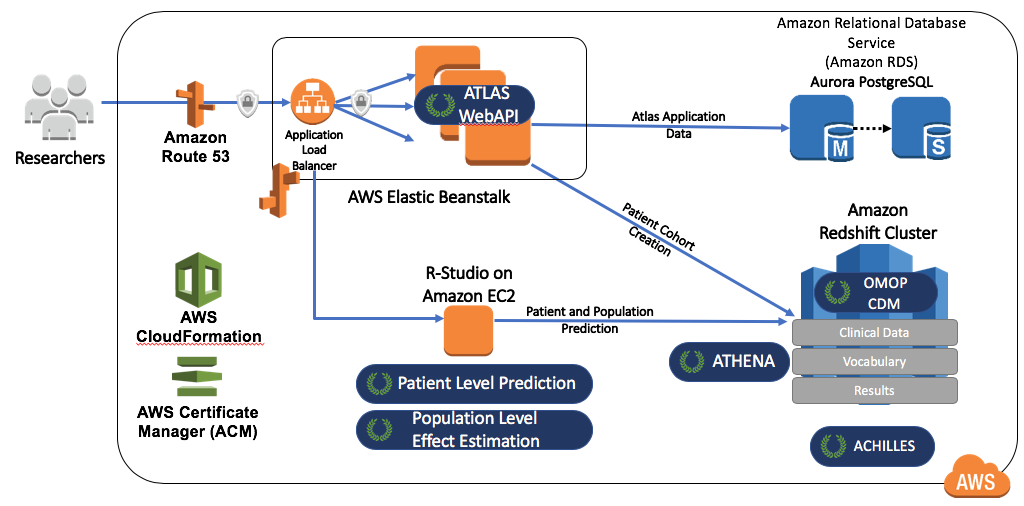
\includegraphics[width=1\linewidth]{images/OhdsiAnalyticsTools/OHDSIonAWSDiagram} 

}

\caption{OHDSIonAWS를 위한 Amazon Web Services 아카이브}\label{fig:ohdsionawsDiagram}
\end{figure}

\section{요약}\label{-6}

\BeginKnitrBlock{rmdsummary}
\begin{itemize}
\tightlist
\item
  다음과 같은 방식으로 CDM 데이터에 대한 분석을 수행할 수 있다.

  \begin{itemize}
  \tightlist
  \item
    사용자가 직접 분석코드 작성
  \item
    OHDSI Method Library에서 R 패키지를 사용하여 코드 작성
  \item
    분석코드 작성없이 대화형 분석 플랫폼 ATLAS를 사용
  \end{itemize}
\item
  OHDSI 툴은 다양한 분석 전략을 사용한다.

  \begin{itemize}
  \tightlist
  \item
    단일 연구
  \item
    실시간 쿼리
  \item
    대규모 분석
  \end{itemize}
\item
  대부분의 OHDSI 분석 툴이 다음에 내장되어 있다.

  \begin{itemize}
  \tightlist
  \item
    대화형 분석 플랫폼 ATLAS
  \item
    OHDSI Methods Library R 패키지
  \end{itemize}
\item
  OHDSI 툴의 구축을 촉진하는 몇 가지 전략이 존재한다.
\end{itemize}
\EndKnitrBlock{rmdsummary}

\chapter{SQL과 R}\label{SqlAndR}

\emph{Chapter leads: Martijn Schuemie \& Peter Rijnbeek}

공통 데이터 모델(Common Data Model, CDM)은 모든 데이터가 필드가 있는
테이블의 레코드로 표시되는 관계형 데이터베이스 모델이다. 이는 일반적으로
PostgreSQL, Oracle, Microsoft SQL Server와 같은 소프트웨어 플랫폼을
사용하여 데이터가 관계형 데이터베이스에 저장된다는 것을 의미한다.
사용자는 ATLAS와 Methods Library 같은 다양한 OHDSI 도구를 통해
데이터베이스에 간접적으로 질의하여 분석을 수행하지만, 적절한 접근 권한이
있으면 이들 도구를 사용하지 않고 직접 데이터베이스에 질의할 수도 있다.
데이터베이스에 직접 질의하는 주된 이유는 현재 기존 도구가 지원하지 않는
분석을 수행하기 위한 것이다. 그러나 OHDSI 도구는 사용자가 데이터를
적절하게 분석을 할 수 있도록 (전문가들이 오랜 시간 고려하여 만든) 지침을
안내하도록 설계되어 있기 때문에 직접 데이터베이스에 질의하는 것은 실수를
범할 위험이 더 커진다. 직접 질의하는 것은 그런 지침을 제공하지 않는다.
관계형 데이터베이스에 질의하기 위한 표준 언어는 Structured Query
Language(SQL)이며, 이는 데이터에 대한 변경뿐만 아니라 데이터베이스에
대한 질의를 위해 사용할 수 있다. SQL의 기본 명령어는 실제로 표준이고
소프트웨어 플랫폼 전반에 걸쳐 같은 의미를 가지지만, 플랫폼마다 미묘한
변경이 있는 고유한 문법을 가지고 있다. 예를 들면, SQL Server에서 PERSON
테이블에서 상위 10개의 행을 검색하려면 다음을 입력한다: \index{SQL}
\index{structured query language|see {SQL}}

\begin{Shaded}
\begin{Highlighting}[]
\KeywordTok{SELECT}\NormalTok{ TOP }\DecValTok{10}\NormalTok{ * }\KeywordTok{FROM}\NormalTok{ person;}
\end{Highlighting}
\end{Shaded}

PostgreSQL의 동일한 질의는 다음과 같다:

\begin{Shaded}
\begin{Highlighting}[]
\KeywordTok{SELECT}\NormalTok{ * }\KeywordTok{FROM}\NormalTok{ person }\KeywordTok{LIMIT} \DecValTok{10}\NormalTok{;}
\end{Highlighting}
\end{Shaded}

OHDSI에서는 플랫폼이 사용하는 고유한 문법에 구애받지 않고 모든 OHDSI
데이터베이스에서 동일한 SQL 언어를 사용하고자 한다. 이러한 이유로
OHDSI는 이 장의 뒤에서 논의하게 될, 하나의 표준 문법을 다른 여러 개의
문법으로 번역해줄 수 있는 패키지인
\href{https://ohdsi.github.io/SqlRender/}{SqlRender}를 개발하였다. 이
표준 언어 - \textbf{OHDSI SQL} - 는 주로 SQL Server SQL 언어의 하위
집합이다. 이 장에서 제공되는 SQL 문에는 모두 OHDSI SQL을 사용한다.
\index{SqlRender} \index{agnostic SQL|see {SqlRender}}
\index{Standard SQL Dialect|see {SqlRender}}
\index{OHDSI SQL|see {SqlRender}}

각 데이터베이스 플랫폼에는 SQL을 사용하여 데이터베이스를 질의하기 위한
자체 소프트웨어 도구가 제공된다. OHDSI는 여러 데이터베이스 플랫폼에
연결할 수 있는 하나의 R 패키지인
\href{https://ohdsi.github.io/DatabaseConnector/}{DatabaseConnector} 를
개발하였다. DatabaseConnector도 이 장의 뒤에서 논의할 것이다.
\index{DatabaseConnector}

따라서 OHDSI 도구를 사용하지 않고도 CDM에 맞게 질의할 수 있지만
DatabaseConnector 및 SqlRender 패키지를 사용하는 것을 권장한다. 이를
통해 한 사이트에서 개발된 질의를 수정하지 않고도 다른 사이트에서 사용할
수 있다. R 자체는 통계 분석 및 대화식 그래프 생성과 같이
데이터베이스에서 추출된 데이터를 추가로 분석하는 기능도 직접 제공한다.
\index{R}

이 장에서는 독자가 SQL에 대한 기본 지식을 가지고 있다고 가정한다. 먼저
SqlRender 및 DatabaseConnector 사용 방법을 검토한다. 독자가 이 패키지를
사용할 의도가 없는 경우 이 절은 건너뛸 수 있다.
\ref{QueryTheCdm}절에서는 SQL(OHDSI SQL)을 사용하여 CDM에 질의하는
방법에 대해 설명한다. 그다음 절에서는 CDM에 질의할 때 OHDSI 표준 용어를
사용하는 방법을 강조한다. 공개적으로 이용 가능한 CDM에 대해 일반적으로
사용되는 질의 모음인 QueryLibrary를 특히 자세히 살펴본다. 발생률을
추정하는 예제 연구로 이 장을 마무리하고 SqlRender 및 DatabaseConnector를
사용하여 이 연구를 구현한다. \index{Query Library}
\index{SQL Query Libary|see {Query Library}}

\hypertarget{SqlRender}{\section{SqlRender}\label{SqlRender}}

\href{https://ohdsi.github.io/SqlRender/}{SqlRender} 패키지는
Comprehensive R Archive Network (CRAN)에서 이용할 수 있으므로 다음을
사용하여 설치할 수 있다:

\begin{Shaded}
\begin{Highlighting}[]
\KeywordTok{install.packages}\NormalTok{(}\StringTok{"SqlRender"}\NormalTok{)}
\end{Highlighting}
\end{Shaded}

SqlRender는 전통적인 데이터베이스 시스템 (PostgreSQL, Microsoft SQL
Server, SQLite, and Oracle), 병렬 데이터 웨어하우스 (Microsoft APS, IBM
Netezza, and Amazon RedShift), 빅데이터 플랫폼 (Hadoop through Impala,
and Google BigQuery) 을 포함한 다수의 기술 플랫폼을 지원한다.

\subsection{SQL의 매개 변수화}\label{sql--}

패키지의 기능 중 하나는 SQL문에 매개 변수를 지원하는 것이다. 일부 매개
변수에 기반하여 SQL문을 조금씩 변형할 필요가 종종 있다. SqlRender는 매개
변수를 허용하기 위해 SQL 코드 내에서 간단한 마크업 구문을 제공한다. 매개
변수를 기반으로 SQL을 렌더링하는 것은 \texttt{render()} 함수를 사용하여
수행한다. \index{SqlRender!parameterization}

\subsubsection*{매개 변수값 대체하기}\label{--}
\addcontentsline{toc}{subsubsection}{매개 변수값 대체하기}

\texttt{@} 문자는 렌더링 시 실제 매개 변수값과 교환해야 하는 매개 변수
이름을 나타내는 데 사용할 수 있다. 다음 예에서 \texttt{a}라고 불리는
변수가 SQL에서 언급되어 있다. 렌더 함수를 호출할 때 이 매개 변수의 값이
정의된다:

\begin{Shaded}
\begin{Highlighting}[]
\NormalTok{sql <-}\StringTok{ "SELECT * FROM concept WHERE concept_id = @a;"}
\KeywordTok{render}\NormalTok{(sql, }\DataTypeTok{a =} \DecValTok{123}\NormalTok{)}
\end{Highlighting}
\end{Shaded}

\begin{verbatim}
## [1] "SELECT * FROM concept WHERE concept_id = 123;"
\end{verbatim}

대부분의 데이터베이스 관리 시스템에서 제공하는 매개 변수와 달리 테이블
또는 필드 이름을 값으로 매개 변수화하기가 쉽다는 것에 주목하라:

\begin{Shaded}
\begin{Highlighting}[]
\NormalTok{sql <-}\StringTok{ "SELECT * FROM @x WHERE person_id = @a;"}
\KeywordTok{render}\NormalTok{(sql, }\DataTypeTok{x =} \StringTok{"observation"}\NormalTok{, }\DataTypeTok{a =} \DecValTok{123}\NormalTok{)}
\end{Highlighting}
\end{Shaded}

\begin{verbatim}
## [1] "SELECT * FROM observation WHERE person_id = 123;"
\end{verbatim}

매개 변수 값은 숫자, 문자열, 부울 및 쉼표를 기준으로 항목을 나눈
리스트로 변환된 벡터일 수 있다:

\begin{Shaded}
\begin{Highlighting}[]
\NormalTok{sql <-}\StringTok{ "SELECT * FROM concept WHERE concept_id IN (@a);"}
\KeywordTok{render}\NormalTok{(sql, }\DataTypeTok{a =} \KeywordTok{c}\NormalTok{(}\DecValTok{123}\NormalTok{, }\DecValTok{234}\NormalTok{, }\DecValTok{345}\NormalTok{))}
\end{Highlighting}
\end{Shaded}

\begin{verbatim}
## [1] "SELECT * FROM concept WHERE concept_id IN (123,234,345);"
\end{verbatim}

\subsubsection*{If-Then-Else}\label{if-then-else}
\addcontentsline{toc}{subsubsection}{If-Then-Else}

때로는 하나 이상의 매개 변수 값에 따라 코드 블록을 켜거나 끌 필요가
있다. 이 작업은
\texttt{\{Condition\}\ ?\ \{if\ true\}\ :\ \{if\ false\}} 구문을
사용한다. \emph{조건}이 참 또는 1로 평가되면, \emph{if true} 블록이
사용되고 그렇지 않으면, \emph{if false} 블록이 표시된다 (있는 경우).

\begin{Shaded}
\begin{Highlighting}[]
\NormalTok{sql <-}\StringTok{ "SELECT * FROM cohort \{@x\} ? \{WHERE subject_id = 1\}"}
\KeywordTok{render}\NormalTok{(sql, }\DataTypeTok{x =} \OtherTok{FALSE}\NormalTok{)}
\end{Highlighting}
\end{Shaded}

\begin{verbatim}
## [1] "SELECT * FROM cohort "
\end{verbatim}

\begin{Shaded}
\begin{Highlighting}[]
\KeywordTok{render}\NormalTok{(sql, }\DataTypeTok{x =} \OtherTok{TRUE}\NormalTok{)}
\end{Highlighting}
\end{Shaded}

\begin{verbatim}
## [1] "SELECT * FROM cohort WHERE subject_id = 1"
\end{verbatim}

간단한 비교도 지원된다:

\begin{Shaded}
\begin{Highlighting}[]
\NormalTok{sql <-}\StringTok{ "SELECT * FROM cohort \{@x == 1\} ? \{WHERE subject_id = 1\};"}
\KeywordTok{render}\NormalTok{(sql, }\DataTypeTok{x =} \DecValTok{1}\NormalTok{)}
\end{Highlighting}
\end{Shaded}

\begin{verbatim}
## [1] "SELECT * FROM cohort WHERE subject_id = 1;"
\end{verbatim}

\begin{Shaded}
\begin{Highlighting}[]
\KeywordTok{render}\NormalTok{(sql, }\DataTypeTok{x =} \DecValTok{2}\NormalTok{)}
\end{Highlighting}
\end{Shaded}

\begin{verbatim}
## [1] "SELECT * FROM cohort ;"
\end{verbatim}

IN 연산자도 지원된다:

\begin{Shaded}
\begin{Highlighting}[]
\NormalTok{sql <-}\StringTok{ "SELECT * FROM cohort \{@x IN (1,2,3)\} ? \{WHERE subject_id = 1\};"}
\KeywordTok{render}\NormalTok{(sql, }\DataTypeTok{x =} \DecValTok{2}\NormalTok{)}
\end{Highlighting}
\end{Shaded}

\begin{verbatim}
## [1] "SELECT * FROM cohort WHERE subject_id = 1;"
\end{verbatim}

\subsection{다른 SQL 언어로의 변환}\label{-sql--}

\href{https://ohdsi.github.io/SqlRender/}{SqlRender} 패키지의 또 다른
기능은 OHDSI SQL에서 다른 SQL 언어로 변환하는 것이다. 예를 들면 다음과
같다:

\begin{Shaded}
\begin{Highlighting}[]
\NormalTok{sql <-}\StringTok{ "SELECT TOP 10 * FROM person;"}
\KeywordTok{translate}\NormalTok{(sql, }\DataTypeTok{targetDialect =} \StringTok{"postgresql"}\NormalTok{)}
\end{Highlighting}
\end{Shaded}

\begin{verbatim}
## [1] "SELECT  * FROM person LIMIT 10;"
\end{verbatim}

\texttt{targetDialect} 매개 변수는 다음과 같은 값을 가질 수 있다:
``oracle'', ``postgresql'', ``pdw'', ``redshift'', ``impala'',
``netezza'', ``bigquery'', ``sqlite'', and ``sql server''.
\index{SqlRender!translation}

\BeginKnitrBlock{rmdimportant}
패키지에는 제한된 변환 규칙 세트만 구현되었기 때문에 SQL의 함수 및
구성을 적절하게 번역되는 것에는 한계가 있을 뿐 아니라 일부 SQL의 특징은
모든 언어에서 동일하지 않다. OHDSI SQL이 독자적인 새로운 문법으로 개발된
주된 이유이다. 하지만 이미 있는 것을 다시 만드느라 쓸데없이 시간을
낭비하지 않기 위해 SQL Server 구문을 유지하였다.
\EndKnitrBlock{rmdimportant}

최선의 노력에도 불구하고, 지원되는 모든 플랫폼에서 오류 없이 실행될
OHDSI SQL을 작성할 때 고려해야 할 사항이 몇 가지 있다. 다음은 이러한
고려 사항에 대해 자세히 설명한다.

\subsubsection*{변환에 의해 지원되는 기능 및 구조}\label{-----}
\addcontentsline{toc}{subsubsection}{변환에 의해 지원되는 기능 및 구조}

다음과 같은 SQL Server 함수는 테스트되었으며 다양한 언어로 올바르게
변환되는 것으로 확인되었다: \index{SqlRender!supported functions}

\begin{longtable}[]{@{}lll@{}}
\caption{\label{tab:sqlFunctions} Functions supported by
translate.}\tabularnewline
\toprule
Function & Function & Function\tabularnewline
\midrule
\endfirsthead
\toprule
Function & Function & Function\tabularnewline
\midrule
\endhead
ABS & EXP & RAND\tabularnewline
ACOS & FLOOR & RANK\tabularnewline
ASIN & GETDATE & RIGHT\tabularnewline
ATAN & HASHBYTES* & ROUND\tabularnewline
AVG & ISNULL & ROW\_NUMBER\tabularnewline
CAST & ISNUMERIC & RTRIM\tabularnewline
CEILING & LEFT & SIN\tabularnewline
CHARINDEX & LEN & SQRT\tabularnewline
CONCAT & LOG & SQUARE\tabularnewline
COS & LOG10 & STDEV\tabularnewline
COUNT & LOWER & SUM\tabularnewline
COUNT\_BIG & LTRIM & TAN\tabularnewline
DATEADD & MAX & UPPER\tabularnewline
DATEDIFF & MIN & VAR\tabularnewline
DATEFROMPARTS & MONTH & YEAR\tabularnewline
DATETIMEFROMPARTS & NEWID &\tabularnewline
DAY & PI &\tabularnewline
EOMONTH & POWER &\tabularnewline
\bottomrule
\end{longtable}

* Oracle은 특별 권한이 필요하다. SQLite에는 해당되는 것이 없다.

마찬가지로 많은 SQL 구문 구조가 지원된다. 다음은 우리가 잘 번역할 수
있는 표현식의 전체 목록이다:

\begin{Shaded}
\begin{Highlighting}[]
\CommentTok{-- Simple selects:}
\KeywordTok{SELECT}\NormalTok{ * }\KeywordTok{FROM} \KeywordTok{table}\NormalTok{;}

\CommentTok{-- Selects with joins:}
\KeywordTok{SELECT}\NormalTok{ * }\KeywordTok{FROM}\NormalTok{ table_1 }\KeywordTok{INNER} \KeywordTok{JOIN}\NormalTok{ table_2 }\KeywordTok{ON}\NormalTok{ a = b;}

\CommentTok{-- Nested queries:}
\KeywordTok{SELECT}\NormalTok{ * }\KeywordTok{FROM}\NormalTok{ (}\KeywordTok{SELECT}\NormalTok{ * }\KeywordTok{FROM}\NormalTok{ table_1) tmp }\KeywordTok{WHERE}\NormalTok{ a = b;}

\CommentTok{-- Limiting to top rows:}
\KeywordTok{SELECT}\NormalTok{ TOP }\DecValTok{10}\NormalTok{ * }\KeywordTok{FROM} \KeywordTok{table}\NormalTok{;}

\CommentTok{-- Selecting into a new table:}
\KeywordTok{SELECT}\NormalTok{ * }\KeywordTok{INTO}\NormalTok{ new_table }\KeywordTok{FROM} \KeywordTok{table}\NormalTok{;}

\CommentTok{-- Creating tables:}
\KeywordTok{CREATE} \KeywordTok{TABLE} \KeywordTok{table}\NormalTok{ (field }\DataTypeTok{INT}\NormalTok{);}

\CommentTok{-- Inserting verbatim values:}
\KeywordTok{INSERT} \KeywordTok{INTO}\NormalTok{ other_table (field_1) }\KeywordTok{VALUES}\NormalTok{ (}\DecValTok{1}\NormalTok{);}

\CommentTok{-- Inserting from SELECT:}
\KeywordTok{INSERT} \KeywordTok{INTO}\NormalTok{ other_table (field_1) }\KeywordTok{SELECT} \FunctionTok{value} \KeywordTok{FROM} \KeywordTok{table}\NormalTok{;}

\CommentTok{-- Simple drop commands:}
\KeywordTok{DROP} \KeywordTok{TABLE} \KeywordTok{table}\NormalTok{;}

\CommentTok{-- Drop table if it exists:}
\KeywordTok{IF}\NormalTok{ OBJECT_ID(}\StringTok{'ACHILLES_analysis'}\NormalTok{, }\StringTok{'U'}\NormalTok{) }\KeywordTok{IS} \KeywordTok{NOT} \KeywordTok{NULL}
  \KeywordTok{DROP} \KeywordTok{TABLE}\NormalTok{ ACHILLES_analysis;}
  
\CommentTok{-- Drop temp table if it exists:}
\KeywordTok{IF}\NormalTok{ OBJECT_ID(}\StringTok{'tempdb..#cohorts'}\NormalTok{, }\StringTok{'U'}\NormalTok{) }\KeywordTok{IS} \KeywordTok{NOT} \KeywordTok{NULL}
  \KeywordTok{DROP} \KeywordTok{TABLE}\NormalTok{ #cohorts;  }

\CommentTok{-- Common table expressions:}
\KeywordTok{WITH}\NormalTok{ cte }\KeywordTok{AS}\NormalTok{ (}\KeywordTok{SELECT}\NormalTok{ * }\KeywordTok{FROM} \KeywordTok{table}\NormalTok{) }\KeywordTok{SELECT}\NormalTok{ * }\KeywordTok{FROM}\NormalTok{ cte;}

\CommentTok{-- OVER clauses:}
\KeywordTok{SELECT} \FunctionTok{ROW_NUMBER}\NormalTok{() }\KeywordTok{OVER}\NormalTok{ (}\KeywordTok{PARTITION} \KeywordTok{BY}\NormalTok{ a }\KeywordTok{ORDER} \KeywordTok{BY}\NormalTok{ b)}
  \KeywordTok{AS} \OtherTok{"Row Number"} \KeywordTok{FROM} \KeywordTok{table}\NormalTok{;}
  
\CommentTok{-- CASE WHEN clauses:}
\KeywordTok{SELECT} \KeywordTok{CASE} \KeywordTok{WHEN}\NormalTok{ a=}\DecValTok{1} \KeywordTok{THEN}\NormalTok{ a }\KeywordTok{ELSE} \DecValTok{0} \KeywordTok{END} \KeywordTok{AS} \FunctionTok{value} \KeywordTok{FROM} \KeywordTok{table}\NormalTok{;}

\CommentTok{-- UNIONs:}
\KeywordTok{SELECT}\NormalTok{ * }\KeywordTok{FROM}\NormalTok{ a }\KeywordTok{UNION} \KeywordTok{SELECT}\NormalTok{ * }\KeywordTok{FROM}\NormalTok{ b;}

\CommentTok{-- INTERSECTIONs:}
\KeywordTok{SELECT}\NormalTok{ * }\KeywordTok{FROM}\NormalTok{ a }\KeywordTok{INTERSECT} \KeywordTok{SELECT}\NormalTok{ * }\KeywordTok{FROM}\NormalTok{ b;}

\CommentTok{-- EXCEPT:}
\KeywordTok{SELECT}\NormalTok{ * }\KeywordTok{FROM}\NormalTok{ a }\KeywordTok{EXCEPT} \KeywordTok{SELECT}\NormalTok{ * }\KeywordTok{FROM}\NormalTok{ b;}
\end{Highlighting}
\end{Shaded}

\subsubsection*{문자열 연결}\label{-}
\addcontentsline{toc}{subsubsection}{문자열 연결}

문자열 연결은 SQL Server가 다른 언어보다 덜 구체적인 영역이다. SQL
Server에서는
\texttt{SELECT\ first\_name\ +\ \textquotesingle{}\ \textquotesingle{}\ +\ last\_name\ AS\ full\_name\ FROM\ table}와
같이 작성하지만 Postgres와 Oracle에서는
\texttt{SELECT\ first\_name\ \textbar{}\textbar{}\ \textquotesingle{}\ \textquotesingle{}\ \textbar{}\textbar{}\ last\_name\ AS\ full\_name\ FROM\ table}
라고 작성한다. SqlRender는 연결되는 값이 문자열인지 추측하려고 한다.
위의 예에서 명시적인 문자열 (작은따옴표로 묶인 공백) 이 있으므로 번역은
정확할 것이다. 그러나
\texttt{SELECT\ first\_name\ +\ last\_name\ AS\ full\_name\ FROM\ table}와
같이 작성한다면 SqlRender는 두 필드가 문자열이라는 단서가 없으며, 잘못된
더하기 기호를 남겼다. 값이 문자열이라는 또 다른 단서는 ``VARCHAR''에
대한 명시적 형변환이므로
\texttt{SELECT\ last\_name\ +\ CAST(age\ AS\ VARCHAR(3))\ AS\ full\_name\ FROM\ table}
도 올바르게 변환된다. 모호성을 피하려면 \texttt{CONCAT()} 함수를
사용하여 두 개 이상의 문자열을 연결하는 것이 가장 좋다.

\subsubsection*{테이블 별칭과 AS 키워드}\label{--as-}
\addcontentsline{toc}{subsubsection}{테이블 별칭과 AS 키워드}

많은 SQL 언어는 테이블 별칭을 정의할 때 \texttt{AS} 키워드를 사용할 수
있지만, 키워드 없이도 잘 동작 한다. 예를 들어, 이 두 SQL 문은 SQL
Server, PostgreSQL, RedShift 등에 적합하다:

\begin{Shaded}
\begin{Highlighting}[]
\CommentTok{-- Using AS keyword}
\KeywordTok{SELECT}\NormalTok{ * }
\KeywordTok{FROM}\NormalTok{ my_table }\KeywordTok{AS}\NormalTok{ table_}\DecValTok{1}
\KeywordTok{INNER} \KeywordTok{JOIN}\NormalTok{ (}
  \KeywordTok{SELECT}\NormalTok{ * }\KeywordTok{FROM}\NormalTok{ other_table}
\NormalTok{) }\KeywordTok{AS}\NormalTok{ table_}\DecValTok{2}
\KeywordTok{ON}\NormalTok{ table_1.person_id = table_2.person_id;}

\CommentTok{-- Not using AS keyword}
\KeywordTok{SELECT}\NormalTok{ * }
\KeywordTok{FROM}\NormalTok{ my_table table_}\DecValTok{1}
\KeywordTok{INNER} \KeywordTok{JOIN}\NormalTok{ (}
  \KeywordTok{SELECT}\NormalTok{ * }\KeywordTok{FROM}\NormalTok{ other_table}
\NormalTok{) table_}\DecValTok{2}
\KeywordTok{ON}\NormalTok{ table_1.person_id = table_2.person_id;}
\end{Highlighting}
\end{Shaded}

그러나 Oracle에서는 \texttt{AS} 키워드를 사용하면 오류가 발생한다. 위의
예제 중 첫 번째 질의는 실패한다. 따라서 테이블 별칭을 지정할 때
\texttt{AS} 키워드를 사용하지 않는 것이 좋다. (참고로 Oracle에서
\texttt{AS}를 사용할 수 없는 테이블 별칭과 이 \texttt{AS}를 사용해야
하는 필드 별칭을 쉽게 구별할 수 없기 때문에 SqlRender가 이 것을
처리하도록 만들 수 없다)

\subsubsection*{임시 테이블}\label{-}
\addcontentsline{toc}{subsubsection}{임시 테이블}

임시 테이블은 중간 결과를 저장하는 데 매우 유용할 수 있으며 올바르게
사용하면 질의 성능을 크게 향상할 수 있다. 대부분의 데이터베이스
플랫폼에서 임시 테이블이라는 매우 좋은 기능을 가지고 있다: 현재
사용자에게만 보이며 세션이 끝나면 자동으로 삭제되고 사용자에게 쓰기
권한이 없어도 생성할 수 있다. 불행히도, Oracle에서는 임시테이블은
기본적으로 영구적인 테이블이며, 데이터의 내부는 현재 사용자에게만
보인다는 차이점만 있다. 이것이 Oracle에서 SqlRender가 다음과 같이 임시
테이블을 에뮬레이션하려고 시도하는 이유이다.

\begin{enumerate}
\def\labelenumi{\arabic{enumi}.}
\tightlist
\item
  테이블 이름에 임의의 문자열을 추가하여 다른 사용자의 테이블이 충돌하지
  않도록 한다.
\item
  사용자가 임시 테이블이 작성될 스키마를 지정할 수 있도록 허용한다.
\end{enumerate}

예를 들면:

\begin{Shaded}
\begin{Highlighting}[]
\NormalTok{sql <-}\StringTok{ "SELECT * FROM #children;"}
\KeywordTok{translate}\NormalTok{(sql, }\DataTypeTok{targetDialect =} \StringTok{"oracle"}\NormalTok{, }\DataTypeTok{oracleTempSchema =} \StringTok{"temp_schema"}\NormalTok{)}
\end{Highlighting}
\end{Shaded}

\begin{verbatim}
## [1] "SELECT * FROM temp_schema.b3k9wfymchildren ;"
\end{verbatim}

사용자는 \texttt{temp\_schema}에 대한 쓰기 권한이 있어야 한다.

또한 Oracle은 테이블 이름이 30자로 제한되어 있다. 세션 아이디를 추가한
후 이름이 너무 길어지기 때문에 \textbf{임시 테이블 이름은 최대
22자까지만 허용된다}.

뿐만 아니라 Oracle의 임시 테이블은 자동 삭제되지 않으므로 Oracle에 임시
테이블 스키마가 쌓이는 것을 방지하기 위해 모든 임시 테이블을 사용한
후에는 명시적으로 \texttt{TRUNCATE} 및 \texttt{DROP} 을 해야 한다.

\subsubsection*{암묵적인 형변환}\label{-}
\addcontentsline{toc}{subsubsection}{암묵적인 형변환}

SQL Server가 다른 언어보다 덜 명시적인 몇 가지 점 중 하나는 암묵적인
형변환을 허용한다는 것이다. 예를 들어 이 코드는 SQL Server에서 작동한다:

\begin{Shaded}
\begin{Highlighting}[]
\KeywordTok{CREATE} \KeywordTok{TABLE}\NormalTok{ #temp (txt }\DataTypeTok{VARCHAR}\NormalTok{);}

\KeywordTok{INSERT} \KeywordTok{INTO}\NormalTok{ #temp}
\KeywordTok{SELECT} \StringTok{'1'}\NormalTok{;}

\KeywordTok{SELECT}\NormalTok{ * }\KeywordTok{FROM}\NormalTok{ #temp }\KeywordTok{WHERE}\NormalTok{ txt = }\DecValTok{1}\NormalTok{;}
\end{Highlighting}
\end{Shaded}

비록 \texttt{txt} 는 VARCHAR 필드이고 이것을 정수와 비교하고 있지만, SQL
Server는 비교를 허용하기 위해 두 가지 중 하나를 자동으로 올바른 타입으로
변환한다. 이와 대조적으로, PostgreSQL과 같은 다른 언어는 VARCHAR와 INT를
비교하려고 할 때 오류를 일으킬 것이다.

따라서 형 변환은 항상 명시적으로 해야 한다. 위의 마지막에 있는 예는

\begin{Shaded}
\begin{Highlighting}[]
\KeywordTok{SELECT}\NormalTok{ * }\KeywordTok{FROM}\NormalTok{ #temp }\KeywordTok{WHERE}\NormalTok{ txt = }\FunctionTok{CAST}\NormalTok{(}\DecValTok{1} \KeywordTok{AS} \DataTypeTok{VARCHAR}\NormalTok{);}
\end{Highlighting}
\end{Shaded}

또는 아래와 같이 대체되어야 한다.

\begin{Shaded}
\begin{Highlighting}[]
\KeywordTok{SELECT}\NormalTok{ * }\KeywordTok{FROM}\NormalTok{ #temp }\KeywordTok{WHERE} \FunctionTok{CAST}\NormalTok{(txt }\KeywordTok{AS} \DataTypeTok{INT}\NormalTok{) = }\DecValTok{1}\NormalTok{;}
\end{Highlighting}
\end{Shaded}

\subsubsection*{문자열 비교의 대소문자 구분}\label{---}
\addcontentsline{toc}{subsubsection}{문자열 비교의 대소문자 구분}

SQL Server와 같은 일부 DBMS 플랫폼은 대소문자를 구분하지 않는 비교를
수행하는 반면, PostgreSQL과 같은 다른 플랫폼은 대소문자를 구분한다.
따라서 항상 대소문자를 구분하는 비교를 가정하고 명확하게 모르는 경우
명시적으로 대소문자를 구분하지 않도록 하는 명령을 추가하여 비교하기
추천한다. 예를 들어,

\begin{Shaded}
\begin{Highlighting}[]
\KeywordTok{SELECT}\NormalTok{ * }\KeywordTok{FROM}\NormalTok{ concept }\KeywordTok{WHERE}\NormalTok{ concep_class_id = }\StringTok{'Clinical Finding'}
\end{Highlighting}
\end{Shaded}

대신, 다음과 같이 사용하는 것이 좋다.

\begin{Shaded}
\begin{Highlighting}[]
\KeywordTok{SELECT}\NormalTok{ * }\KeywordTok{FROM}\NormalTok{ concept }\KeywordTok{WHERE} \FunctionTok{LOWER}\NormalTok{(concep_class_id) = }\StringTok{'clinical finding'}
\end{Highlighting}
\end{Shaded}

\subsubsection*{스키마와 데이터베이스}\label{-}
\addcontentsline{toc}{subsubsection}{스키마와 데이터베이스}

SQL Server에서 테이블은 스키마안에 있으며 스키마는 데이터베이스 안에
있다. 예를 들면, \texttt{cdm\_data.dbo.person}은 \texttt{cdm\_data}
데이터베이스의 \texttt{dbo} 스키마 안에 있는 \texttt{person} 테이블을
말한다. 다른 언어에서는 비슷한 계층 구조가 종종 존재하더라도 매우 다르게
사용된다. SQL Server에는 일반적으로 데이터베이스 당 하나의 스키마
(\texttt{dbo}라고 함), 가 있으며 사용자는 다른 데이터베이스의 데이터를
쉽게 사용할 수 있다. Postgres와 같은 다른 플랫폼에서는 단일 세션에서
데이터베이스 간 데이터를 사용할 수 없지만, 데이터베이스 안에는 많은
스키마를 가지고 있다. SQL Server의 데이터베이스는 PostgreSQL에서
스키마라고 할 수 있다.

따라서 SQL Server의 데이터베이스와 스키마를 단일 매개변수로 연결할 것을
권장한다. 이 매개 변수는 일반적으로 \texttt{@databaseSchema} 라고 한다.
예를 들면 우리는 매개 변수화된 SQL을 가질 수 있다.

\begin{Shaded}
\begin{Highlighting}[]
\KeywordTok{SELECT}\NormalTok{ * }\KeywordTok{FROM}\NormalTok{ @databaseSchema.person}
\end{Highlighting}
\end{Shaded}

SQL Server에서 \texttt{databaseSchema\ =\ "cdm\_data.dbo"}값에
데이터베이스와 스키마이름을 모두 포함할 수 있다. 다른 플랫폼에서는
동일한 코드를 사용할 수 있지만, 스키마 매개 변수 값은 다음과 같이
지정한다: \texttt{databaseSchema\ =\ "cdm\_data"}

이것이 실패하는 한 가지 상황은 에러를 발생시키는
\texttt{USE\ cdm\_data.dbo;}, 즉 \texttt{USE} 명령어를 사용했기
때문이다. 따라서 \texttt{USE} 명령어를 사용하지 말고 항상 테이블이 있는
데이터베이스 및 스키마를 지정하는 것이 바람직하다.

\subsubsection*{매개 변수화 된 SQL 디버깅하기}\label{---sql-}
\addcontentsline{toc}{subsubsection}{매개 변수화 된 SQL 디버깅하기}

매개 변수화된 SQL을 디버깅하는 것은 약간 복잡할 수 있다. 렌더링 된 SQL만
데이터베이스 서버에 대해 테스트할 수 있지만 매개 변수화된 (사전 렌더링
된) SQL에서 코드를 변경해야 한다. \index{SqlRender!debugging}

SqlRender 패키지에는 대화형으로 SQL소스를 편집하여 SQL을 랜더링을 하거나
반대로 번역할 수 있는 샤이니 앱이 포함되어 있다. 이 앱은 다음과 같이
시작한다:

\begin{Shaded}
\begin{Highlighting}[]
\KeywordTok{launchSqlRenderDeveloper}\NormalTok{()}
\end{Highlighting}
\end{Shaded}

그러면 그림 \ref{fig:sqlDeveloper}에 표시된 앱으로 기본 브라우저가
열린다. 이 앱은 웹에서도 공개적으로 사용할 수 있다.\footnote{\url{http://data.ohdsi.org/SqlDeveloper/}}

\begin{figure}

{\centering 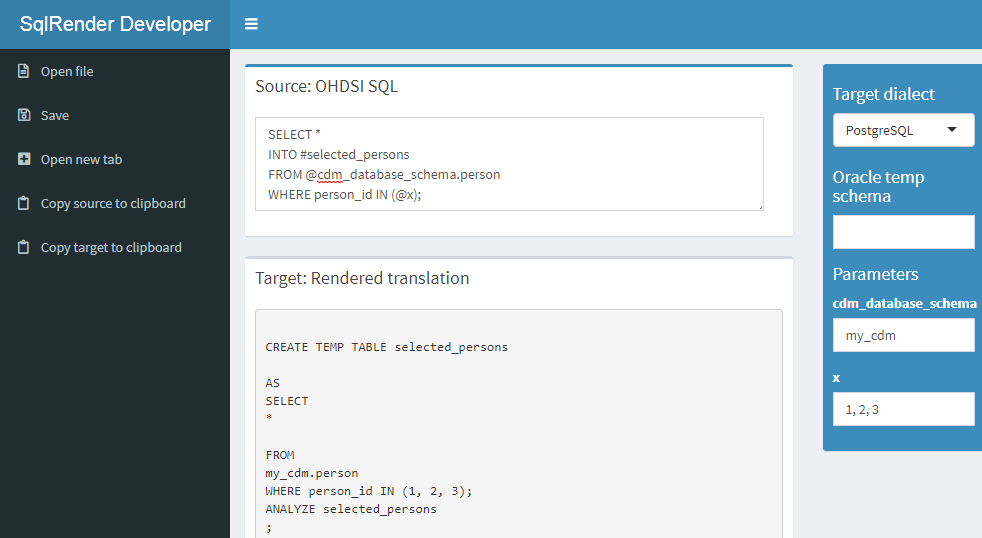
\includegraphics[width=1\linewidth]{images/SqlAndR/sqlDeveloper} 

}

\caption{The SqlDeveloper Shiny 앱.}\label{fig:sqlDeveloper}
\end{figure}

앱에서 OHDSI SQL을 입력하고 대상 언어를 선택하고 SQL에 매개 변수 값을
제공하면 자동으로 번역된 SQL이 하단에 나타난다.

\hypertarget{DatabaseConnector}{\section{DatabaseConnector}\label{DatabaseConnector}}

\href{https://ohdsi.github.io/DatabaseConnector/}{DatabaseConnector} 는
Java의 JDBC 드라이버를 사용하여 다양한 데이터베이스 플랫폼에 연결하기
위한 R 패키지이다. DatabaseConnector 패키지는 CRAN (종합 R 아카이브
네트워크) 에서 사용할 수 있으므로 다음을 사용하여 설치할 수 있다:

\begin{Shaded}
\begin{Highlighting}[]
\KeywordTok{install.packages}\NormalTok{(}\StringTok{"DatabaseConnector"}\NormalTok{)}
\end{Highlighting}
\end{Shaded}

DatabaseConnector는 기존 데이터베이스 시스템 (PostgreSQL, Microsoft SQL
Server, SQLite 및 Oracle), 병렬 데이터웨어 하우스 (Microsoft APS, IBM
Netezza 및 Amazon RedShift) 및 빅데이터 플랫폼 (Hadoop through Impla 및
Google BigQuery) 을 포함한 다양한 기술 플랫폼을 지원한다. 패키지에는
이미 대부분의 드라이버가 포함되어 있지만, 라이센스 문제로 인해 BigQuery,
Netezza 및 Impla 용 드라이버는 포함되어 있지 않아서 사용자가 구해야
한다. 이러한 드라이버를 다운로드하는 방법에 대한 지침을 보려면
\texttt{?jdbcDrivers} 를 입력한다. 다운로드한 후 \texttt{connect},
\texttt{dbConnect}, and \texttt{createConnectionDetails} 함수의
\texttt{pathToDriver} 인수로 사용할 수 있다.

\subsection{연결 생성하기}\label{-}

데이터베이스에 연결하려면 데이터베이스 플랫폼, 서버의 위치, 사용자 이름
및 비밀번호와 같은 많은 세부 사항을 지정해야 한다. \texttt{connect}
함수를 호출하여 다음 세부 사항을 직접 지정할 수 있다:
\index{DatabaseConnector!creating a connection}

\begin{Shaded}
\begin{Highlighting}[]
\NormalTok{conn <-}\StringTok{ }\KeywordTok{connect}\NormalTok{(}\DataTypeTok{dbms =} \StringTok{"postgresql"}\NormalTok{,}
                \DataTypeTok{server =} \StringTok{"localhost/postgres"}\NormalTok{,}
                \DataTypeTok{user =} \StringTok{"joe"}\NormalTok{,}
                \DataTypeTok{password =} \StringTok{"secret"}\NormalTok{,}
                \DataTypeTok{schema =} \StringTok{"cdm"}\NormalTok{)}
\end{Highlighting}
\end{Shaded}

\begin{verbatim}
## Connecting using PostgreSQL driver
\end{verbatim}

각 플랫폼에 필요한 세부 사항에 대한 정보는 \texttt{?connect} 를
참조하라. 나중에 작업을 마치고 연결 끊는 것을 잊지 말라:

\begin{Shaded}
\begin{Highlighting}[]
\KeywordTok{disconnect}\NormalTok{(conn)}
\end{Highlighting}
\end{Shaded}

서버 이름을 제공하는 대신 JDBC connecting string을 사용하는 것이 더
편리할 경우 이를 제공할 수도 있다는 점에 유의하라:

\begin{Shaded}
\begin{Highlighting}[]
\NormalTok{connString <-}\StringTok{ "jdbc:postgresql://localhost:5432/postgres"}
\NormalTok{conn <-}\StringTok{ }\KeywordTok{connect}\NormalTok{(}\DataTypeTok{dbms =} \StringTok{"postgresql"}\NormalTok{,}
                \DataTypeTok{connectionString =}\NormalTok{ connString,}
                \DataTypeTok{user =} \StringTok{"joe"}\NormalTok{,}
                \DataTypeTok{password =} \StringTok{"secret"}\NormalTok{,}
                \DataTypeTok{schema =} \StringTok{"cdm"}\NormalTok{)}
\end{Highlighting}
\end{Shaded}

\begin{verbatim}
## Connecting using PostgreSQL driver
\end{verbatim}

때때로 먼저 세부 사항을 지정하고 나중에 연결할 때까지 연결을 연기해야 할
수 있다. 예를 들어, 함수 내에서 연결이 설정되고 세부 사항은 인수로
전달해야 하는 경우에 편리할 수 있다. 이를 목적으로
\texttt{createConnectionDetails} 함수를 사용할 수 있다:

\begin{Shaded}
\begin{Highlighting}[]
\NormalTok{details <-}\StringTok{ }\KeywordTok{createConnectionDetails}\NormalTok{(}\DataTypeTok{dbms =} \StringTok{"postgresql"}\NormalTok{,}
                                   \DataTypeTok{server =} \StringTok{"localhost/postgres"}\NormalTok{,}
                                   \DataTypeTok{user =} \StringTok{"joe"}\NormalTok{,}
                                   \DataTypeTok{password =} \StringTok{"secret"}\NormalTok{,}
                                   \DataTypeTok{schema =} \StringTok{"cdm"}\NormalTok{)}
\NormalTok{conn <-}\StringTok{ }\KeywordTok{connect}\NormalTok{(details)}
\end{Highlighting}
\end{Shaded}

\begin{verbatim}
## Connecting using PostgreSQL driver
\end{verbatim}

\subsection{질의하기}

데이터베이스 질의를 위한 주요 함수는 \texttt{querySql}과
\texttt{executeSql} 이다. 이러한 함수의 차이점은 \texttt{querySql}은
데이터베이스가 데이터를 반환할 것으로 예상하며, 한 번에 하나의 SQL 문만
처리할 수 있다는 것이다. 이와 대조적으로 \texttt{executeSql}은 데이터를
반환할 것을 예상하지 않으며, 단일 SQL 문자열에서 복수의 SQL 문을
수용한다. \index{DatabaseConnector!querying}

몇가지 예시:

\begin{Shaded}
\begin{Highlighting}[]
\KeywordTok{querySql}\NormalTok{(conn, }\StringTok{"SELECT TOP 3 * FROM person"}\NormalTok{)}
\end{Highlighting}
\end{Shaded}

\begin{verbatim}
##   person_id gender_concept_id year_of_birth
## 1         1              8507          1975
## 2         2              8507          1976
## 3         3              8507          1977
\end{verbatim}

\begin{Shaded}
\begin{Highlighting}[]
\KeywordTok{executeSql}\NormalTok{(conn, }\StringTok{"TRUNCATE TABLE foo; DROP TABLE foo;"}\NormalTok{)}
\end{Highlighting}
\end{Shaded}

두 함수 모두 광범위한 오류보고 기능을 제공한다: 서버에서 오류가 발생하면
오류 메시지와 문제가 되는 SQL 부분이 텍스트 파일에 기록되어 더 나은
디버깅을 돕는다. 기본적으로 \texttt{executeSql} 함수도 실행 된 SQL 문의
백분율을 나타내는 진행 표시 줄을 보여준다. 이러한 속성이 필요하지 않은
경우 패키지는 \texttt{lowLevelQuerySql}과 \texttt{lowLevelExecuteSql}
함수도 제공한다.

\subsection{Ffdf 객체를 사용하여 질의하기}\label{ffdf---}

데이터베이스에서 가져올 데이터가 너무 커서 종종 메모리에 들어갈 수 없는
경우도 있다. \ref{BigDataSupport}절에서 언급했듯이, 그러한 경우
\texttt{ff} 패키지를 사용하여 R 데이터 객체를 디스크에 저장하고
메모리에서 사용하듯이 사용할 수 있다. \texttt{DatabaseConnector}는
객체에 데이터를 직접 다운로드할 수 있다:

\begin{Shaded}
\begin{Highlighting}[]
\NormalTok{x <-}\StringTok{ }\KeywordTok{querySql.ffdf}\NormalTok{(conn, }\StringTok{"SELECT * FROM person"}\NormalTok{)}
\end{Highlighting}
\end{Shaded}

x는 이제 ffdf 객체이다.

\subsection{같은 SQL을 사용하여 다른 플랫폼 질의하기}\label{-sql----}

SqlRender 패키지의 \texttt{render} 및 \texttt{translate} 함수를 먼저
호출하는 다음과 같은 편의 함수를 사용할 수 있다:
\texttt{renderTranslateExecuteSql}, \texttt{renderTranslateQuerySql},
\texttt{renderTranslateQuerySql.ffdf}. 예를 들면:

\begin{Shaded}
\begin{Highlighting}[]
\NormalTok{x <-}\StringTok{ }\KeywordTok{renderTranslateQuerySql}\NormalTok{(conn, }
                             \DataTypeTok{sql =} \StringTok{"SELECT TOP 10 * FROM @schema.person"}\NormalTok{,}
                             \DataTypeTok{schema =} \StringTok{"cdm_synpuf"}\NormalTok{)}
\end{Highlighting}
\end{Shaded}

SQL Server 관련 `TOP 10' 구문은 PostgreSQL에서 예를 들어 `LIMIT 10'으로
변환되며 SQL 매개변수 \texttt{@schema} 는 제공된 값 `cdm\_synpuf'로
인스턴스화 되는 것에 주의해야한다.

\subsection{테이블 삽입하기}\label{-}

\texttt{executeSql} 함수를 사용하여 SQL 문을 전송하여 데이터베이스에
데이터를 삽입할 수도 있지만, \texttt{insertTable} 함수를 사용하는 것이
더 편리하고 빠르다 (일부 최적화로 인해):

\begin{Shaded}
\begin{Highlighting}[]
\KeywordTok{data}\NormalTok{(mtcars)}
\KeywordTok{insertTable}\NormalTok{(conn, }\StringTok{"mtcars"}\NormalTok{, mtcars, }\DataTypeTok{createTable =} \OtherTok{TRUE}\NormalTok{)}
\end{Highlighting}
\end{Shaded}

이 예는 mtcars 데이터 프레임을 자동으로 서버의 'mtcars'라는 테이블로
업로드하고 생성한다.

\section{CDM 질의하기}\label{QueryTheCdm}

다음 예시에서는 CDM이 적용된 데이터베이스를 질의하기 위해 OHDSI SQL을
사용한다. 이러한 쿼리는 CDM의 데이터를 찾을 수 있는 데이터베이스
스키마를 나타내기 위해 \texttt{@cdm}을 사용한다.

데이터베이스에 얼마나 많은 사람이 있는지 질의하는 것부터 시작할 수 있다:

\begin{Shaded}
\begin{Highlighting}[]
\KeywordTok{SELECT} \FunctionTok{COUNT}\NormalTok{(*) }\KeywordTok{AS}\NormalTok{ person_count }\KeywordTok{FROM}\NormalTok{ @cdm.person;}
\end{Highlighting}
\end{Shaded}

\begin{longtable}[]{@{}r@{}}
\toprule
PERSON\_COUNT\tabularnewline
\midrule
\endhead
26299001\tabularnewline
\bottomrule
\end{longtable}

그렇지 않으면 observation period의 평균에 관심이 있을 수도 있다:

\begin{Shaded}
\begin{Highlighting}[]
\KeywordTok{SELECT} \FunctionTok{AVG}\NormalTok{(DATEDIFF(}\DataTypeTok{DAY}\NormalTok{, }
\NormalTok{                    observation_period_start_date, }
\NormalTok{                    observation_period_end_date) / }\FloatTok{365.25}\NormalTok{) }\KeywordTok{AS}\NormalTok{ num_years}
\KeywordTok{FROM}\NormalTok{ @cdm.observation_period;}
\end{Highlighting}
\end{Shaded}

\begin{longtable}[]{@{}r@{}}
\toprule
NUM\_YEARS\tabularnewline
\midrule
\endhead
1.980803\tabularnewline
\bottomrule
\end{longtable}

테이블을 조인하여 추가 통계를 생성할 수 있다. 조인은 일반적으로 테이블의
특정 필드가 동일한 값을 갖도록 하여 여러 테이블의 필드를 결합한다. 예를
들어 두 테이블 모두 가지고 있는 PERSON\_ID 필드로 PERSON 테이블과
OBSERVATION\_PEROPD 테이블을 조인할 수 있다. 즉, 조인의 결과는 두
테이블의 모든 필드를 갖는 새로운 테이블과 같은 집합이지만, 모든 행에서
두 테이블의 PERSON\_ID는 동일한 값을 가져야 한다. 예를 들어 PERSON
테이블의 YEAR\_OF\_BIRTH 필드와 함께 OBSERVATION\_PERIOD 테이블의
OBSERVATION\_PERIOD\_END\_DATE 필드를 사용하여 관찰 종료시 환자의 최고
나이를 계산할 수 있다:

\begin{Shaded}
\begin{Highlighting}[]
\KeywordTok{SELECT} \FunctionTok{MAX}\NormalTok{(}\DataTypeTok{YEAR}\NormalTok{(observation_period_end_date) -}
\NormalTok{           year_of_birth) }\KeywordTok{AS}\NormalTok{ max_age}
\KeywordTok{FROM}\NormalTok{ @cdm.person}
\KeywordTok{INNER} \KeywordTok{JOIN}\NormalTok{ @cdm.observation_period}
  \KeywordTok{ON}\NormalTok{ person.person_id = observation_period.person_id;}
\end{Highlighting}
\end{Shaded}

\begin{longtable}[]{@{}r@{}}
\toprule
MAX\_AGE\tabularnewline
\midrule
\endhead
90\tabularnewline
\bottomrule
\end{longtable}

관찰 시작 당시 연령 분포를 결정하려면 훨씬 더 복잡한 질의가 필요하다. 이
질의에서는 먼저 PERSON 테이블과 OBSERVATION\_PERIOD을 조인하여 관찰 당시
연령을 계산한다. 또한 연령을 기준으로 이 조인된 집합의 순서를 정렬하고
order\_nr로 저장한다. 이 조인의 결과를 여러 번 사용하고 싶기 때문에
``ages''라고 하는 common table expression (CTE)
(\texttt{WITH\ ...\ AS}를 사용하여 정의된) 으로 정의한다. 즉, 연령을
기존 테이블인 것처럼 나타낼 수 있다. ``ages''의 행 수를 세어 ``n''을
생성하고 각 사분위수에 대해 order\_nr이 분수 시간 ``n,'' 보다 작은 최소
연령을 찾는다. 예를 들어, 중앙값을 찾기 위해 \(order\_nr < .50 * n\)인
최소 연령을 사용한다. 최소 및 최대 연령은 별도로 계산된다:

\begin{Shaded}
\begin{Highlighting}[]
\KeywordTok{WITH}\NormalTok{ ages}
\KeywordTok{AS}\NormalTok{ (}
    \KeywordTok{SELECT}\NormalTok{ age,}
        \FunctionTok{ROW_NUMBER}\NormalTok{() }\KeywordTok{OVER}\NormalTok{ (}
            \KeywordTok{ORDER} \KeywordTok{BY}\NormalTok{ age}
\NormalTok{            ) order_nr}
    \KeywordTok{FROM}\NormalTok{ (}
        \KeywordTok{SELECT} \DataTypeTok{YEAR}\NormalTok{(observation_period_start_date) - year_of_birth }\KeywordTok{AS}\NormalTok{ age}
        \KeywordTok{FROM}\NormalTok{ @cdm.person}
        \KeywordTok{INNER} \KeywordTok{JOIN}\NormalTok{ @cdm.observation_period}
            \KeywordTok{ON}\NormalTok{ person.person_id = observation_period.person_id}
\NormalTok{        ) age_computed}
\NormalTok{    )}
\KeywordTok{SELECT} \FunctionTok{MIN}\NormalTok{(age) }\KeywordTok{AS}\NormalTok{ min_age,}
    \FunctionTok{MIN}\NormalTok{(}\KeywordTok{CASE} 
            \KeywordTok{WHEN}\NormalTok{ order_nr < .}\DecValTok{25}\NormalTok{ * n}
                \KeywordTok{THEN} \DecValTok{9999}
            \KeywordTok{ELSE}\NormalTok{ age}
            \KeywordTok{END}\NormalTok{) }\KeywordTok{AS}\NormalTok{ q25_age,}
    \FunctionTok{MIN}\NormalTok{(}\KeywordTok{CASE} 
            \KeywordTok{WHEN}\NormalTok{ order_nr < .}\DecValTok{50}\NormalTok{ * n}
                \KeywordTok{THEN} \DecValTok{9999}
            \KeywordTok{ELSE}\NormalTok{ age}
            \KeywordTok{END}\NormalTok{) }\KeywordTok{AS}\NormalTok{ median_age,}
    \FunctionTok{MIN}\NormalTok{(}\KeywordTok{CASE} 
            \KeywordTok{WHEN}\NormalTok{ order_nr < .}\DecValTok{75}\NormalTok{ * n}
                \KeywordTok{THEN} \DecValTok{9999}
            \KeywordTok{ELSE}\NormalTok{ age}
            \KeywordTok{END}\NormalTok{) }\KeywordTok{AS}\NormalTok{ q75_age,}
    \FunctionTok{MAX}\NormalTok{(age) }\KeywordTok{AS}\NormalTok{ max_age}
\KeywordTok{FROM}\NormalTok{ ages}
\KeywordTok{CROSS} \KeywordTok{JOIN}\NormalTok{ (}
    \KeywordTok{SELECT} \FunctionTok{COUNT}\NormalTok{(*) }\KeywordTok{AS}\NormalTok{ n}
    \KeywordTok{FROM}\NormalTok{ ages}
\NormalTok{    ) population_size;}
\end{Highlighting}
\end{Shaded}

\begin{longtable}[]{@{}rrrrr@{}}
\toprule
MIN\_AGE & Q25\_AGE & MEDIAN\_AGE & Q75\_AGE & MAX\_AGE\tabularnewline
\midrule
\endhead
0 & 6 & 17 & 34 & 90\tabularnewline
\bottomrule
\end{longtable}

SQL을 사용하는 대신 R에서 더 복잡한 계산을 수행할 수도 있다. 예를 들어,
이 코드를 사용하여 동일한 결과를 얻을 수 있다:

\begin{Shaded}
\begin{Highlighting}[]
\NormalTok{sql <-}\StringTok{ "SELECT YEAR(observation_period_start_date) -}
\StringTok{               year_of_birth AS age}
\StringTok{FROM @cdm.person}
\StringTok{INNER JOIN @cdm.observation_period}
\StringTok{  ON person.person_id = observation_period.person_id;"}
\NormalTok{age <-}\StringTok{ }\KeywordTok{renderTranslateQuerySql}\NormalTok{(conn, sql, }\DataTypeTok{cdm =} \StringTok{"cdm"}\NormalTok{)}
\KeywordTok{quantile}\NormalTok{(age[, }\DecValTok{1}\NormalTok{], }\KeywordTok{c}\NormalTok{(}\DecValTok{0}\NormalTok{, }\FloatTok{0.25}\NormalTok{, }\FloatTok{0.5}\NormalTok{, }\FloatTok{0.75}\NormalTok{, }\DecValTok{1}\NormalTok{))}
\end{Highlighting}
\end{Shaded}

\begin{verbatim}
##   0%  25%  50%  75% 100% 
##    0    6   17   34   90
\end{verbatim}

서버에서 연령을 계산하고 모든 연령들을 다운로드한 다음 연령 분포를
계산한다. 그러나 이를 위해서는 데이터베이스 서버에서 수백만 행의
데이터를 다운로드해야 하므로 효율성이 떨어진다. 계산이 SQL에서 가장 잘
수행되는지 R에서 가장 잘 수행되는지의 여부를 사례별로 결정해야 한다.

질의는 CDM의 source value를 사용할 수도 있다. 예를 들어, 다음을 사용하여
가장 빈번한 상위 10개의 condition source code를 검색할 수 있다:

\begin{Shaded}
\begin{Highlighting}[]
\KeywordTok{SELECT}\NormalTok{ TOP }\DecValTok{10}\NormalTok{ condition_source_value, }
  \FunctionTok{COUNT}\NormalTok{(*) }\KeywordTok{AS}\NormalTok{ code_count}
\KeywordTok{FROM}\NormalTok{ @cdm.condition_occurrence}
\KeywordTok{GROUP} \KeywordTok{BY}\NormalTok{ condition_source_value}
\KeywordTok{ORDER} \KeywordTok{BY}\NormalTok{ -COUNT(*);}
\end{Highlighting}
\end{Shaded}

\begin{longtable}[]{@{}rr@{}}
\toprule
CONDITION\_SOURCE\_VALUE & CODE\_COUNT\tabularnewline
\midrule
\endhead
4019 & 49094668\tabularnewline
25000 & 36149139\tabularnewline
78099 & 28908399\tabularnewline
319 & 25798284\tabularnewline
31401 & 22547122\tabularnewline
317 & 22453999\tabularnewline
311 & 19626574\tabularnewline
496 & 19570098\tabularnewline
I10 & 19453451\tabularnewline
3180 & 18973883\tabularnewline
\bottomrule
\end{longtable}

여기서 CONDITION\_OCCURRENCE 테이블의 행을 CONDITION\_SOURCE\_VALUE
필드의 값으로 그룹화하고 각 그룹의 행 수를 세었다. 우리는
CONDITION\_SOURCE\_VALUE, count, 그리고 count의 역순을 검색했다.

\section{질의할 때 Vocabulary 사용하기}\label{--vocabulary-}

많은 작업에서 Vocabulary는 유용하다. Vocabulary 테이블은 CDM의
일부이므로 SQL 쿼리를 사용하여 이용할 수 있다. Vocabulary에 대한 질의가
CDM에 대한 질의와 어떻게 결합할 수 있는지 보여준다. CDM의 많은 필드에는
CONCEPT 테이블을 사용하여 확인할 수 있는 concept ID들이 포함되어 있다.
예를 들어, 데이터베이스에서 성별에 따라 계층화된 인원수를 셀려고 할때,
GENDER\_CONCEPT\_ID를 concept name으로 찾아 바꾸어 사용하는 것이 더
편리할 것이다:

\begin{Shaded}
\begin{Highlighting}[]
\KeywordTok{SELECT} \FunctionTok{COUNT}\NormalTok{(*) }\KeywordTok{AS}\NormalTok{ subject_count,}
\NormalTok{  concept_name}
\KeywordTok{FROM}\NormalTok{ @cdm.person}
\KeywordTok{INNER} \KeywordTok{JOIN}\NormalTok{ @cdm.concept}
  \KeywordTok{ON}\NormalTok{ person.gender_concept_id = concept.concept_id}
\KeywordTok{GROUP} \KeywordTok{BY}\NormalTok{ concept_name;}
\end{Highlighting}
\end{Shaded}

\begin{longtable}[]{@{}rr@{}}
\toprule
SUBJECT\_COUNT & CONCEPT\_NAME\tabularnewline
\midrule
\endhead
14927548 & FEMALE\tabularnewline
11371453 & MALE\tabularnewline
\bottomrule
\end{longtable}

Vocabulary의 매우 강력한 특징은 계층구조에 있다. 특정 개념과 그에 속하는
\emph{모든 하위 개념}을 찾는 쿼리를 사용하는 경우가 빈번하다. 예를 들어,
ibuprofen 성분이 들어 있는 처방전의 수를 세고 싶다고 상상해보라:

\begin{Shaded}
\begin{Highlighting}[]
\KeywordTok{SELECT} \FunctionTok{COUNT}\NormalTok{(*) }\KeywordTok{AS}\NormalTok{ prescription_count}
\KeywordTok{FROM}\NormalTok{ @cdm.drug_exposure}
\KeywordTok{INNER} \KeywordTok{JOIN}\NormalTok{ @cdm.concept_ancestor}
  \KeywordTok{ON}\NormalTok{ drug_concept_id = descendant_concept_id}
\KeywordTok{INNER} \KeywordTok{JOIN}\NormalTok{ @cdm.concept ingredient}
  \KeywordTok{ON}\NormalTok{ ancestor_concept_id = ingredient.concept_id}
\KeywordTok{WHERE} \FunctionTok{LOWER}\NormalTok{(ingredient.concept_name) = }\StringTok{'ibuprofen'}
  \KeywordTok{AND}\NormalTok{ ingredient.concept_class_id = }\StringTok{'Ingredient'}
  \KeywordTok{AND}\NormalTok{ ingredient.standard_concept = }\StringTok{'S'}\NormalTok{;}
\end{Highlighting}
\end{Shaded}

\begin{longtable}[]{@{}r@{}}
\toprule
PRESCRIPTION\_COUNT\tabularnewline
\midrule
\endhead
26871214\tabularnewline
\bottomrule
\end{longtable}

\section{QueryLibrary}\label{querylibrary}

\index{QueryLibrary}

QueryLibrary는 CDM에 대해 일반적으로 사용되는 SQL 질의들의
라이브러리이다. 그림 \ref{fig:queryLibrary}에 표시된 응용
프로그램\footnote{\url{http://data.ohdsi.org/QueryLibrary}} 및 R
패키지로 제공된다.\footnote{\url{https://github.com/OHDSI/QueryLibrary}}

\begin{figure}

{\centering 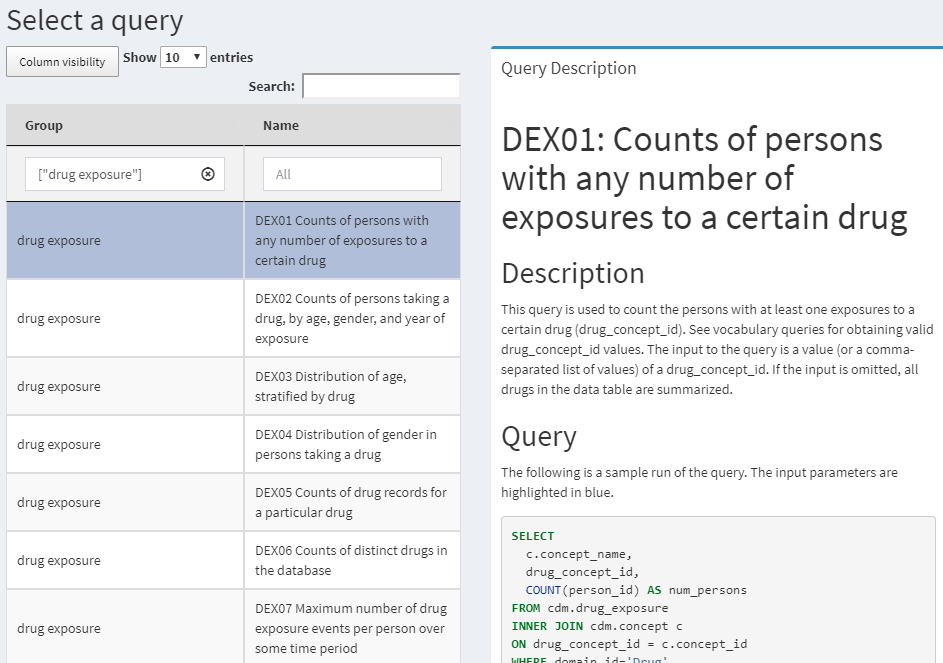
\includegraphics[width=1\linewidth]{images/SqlAndR/queryLibrary} 

}

\caption{QueryLibrary: CDM에 대한 SQL 조회 라이브러리.}\label{fig:queryLibrary}
\end{figure}

라이브러리의 목적은 새로운 사용자가 CDM에 질의하는 방법을 배우도록 돕는
것이다. 라이브러리의 질의는 OHDSI 커뮤니티에서 검토하고 승인하였다. 질의
라이브러리는 주로 교육 목적으로 사용되지만 숙련된 사용자에게 유용한
자원이기도 하다.

QueryLibrary는 SqlRender를 사용하여 선택한 SQL 언어로 질의를 출력한다.
사용자는 CDM 데이터베이스 스키마, vocabulary 데이터베이스 스키마 (별도의
경우) 및 Oracle 임시 스키마 (필요한 경우) 를 지정할 수 있으므로 이러한
설정으로 질의가 자동으로 렌더링 된다.

\section{간단한 연구 구성하기}\label{--}

\subsection{문제 정의}\label{-}

Angioedema(혈관 부종)은 ACE inhibitor(ACEi)의 잘 알려진 부작용이다.
\citep{slater_1988} ACEi 치료 첫 주에 혈관 부종의 발생률이 주당
3,000명의 환자당 1건인 것으로 추정하였다. 여기서 우리는 이 결론을
모방하고 연령과 성별에 따라 계층화한다. 간단하게 하기 위해서 우리는
하나의 ACEi: lisinopril에 중점을 둔다. 따라서 우리는 질문에 대답한다.

\begin{quote}
Lisinopril 치료 개시 후 첫 주에 연령과 성별에 따라 계층화되는 혈관
부종의 비율은 얼마인가?
\end{quote}

\subsection{노출}

Exposure(노출)은 lisinopril에 대한 첫번째 노출로 정의한다. 먼저 이전에
lisinopril에 노출되지 않았음을 의미한다. 첫 노출 전에 365 일의 연속 관찰
기간이 필요하다.

\subsection{결과}

입원 또는 응급실 방문 중 혈관 부종 진단 코드의 발생으로 혈관 부종을
정의한다.

\subsection{위험 노출 기간 (Time-at-risk)}\label{---time-at-risk}

환자가 일주일 동안 노출되었는지 여부와 관계없이 이 치료 시작 후 첫 주에
발생률을 계산한다.

\section{SQL과 R을 사용하여 연구 구현}\label{sql-r---}

OHDSI 툴 규약에 구속되지 않지만 동일한 원칙을 따르는 것은 도움이 된다.
이 경우 OHDSI 툴의 작동 방식과 유사하게 SQL을 사용하여 코호트 테이블을
채운다. 코호트 테이블은 CDM에 정의되어 있으며 사전 정의된 필드 집합도
있다. 먼저 쓰기 접근 권한이 있는 데이터베이스 스키마에 COHORT 테이블을
만들어야 하는데, 이는 CDM 형식으로 데이터를 저장하는 데이터베이스
스키마와 동일하지 않을 수 있다.

\begin{Shaded}
\begin{Highlighting}[]
\KeywordTok{library}\NormalTok{(DatabaseConnector)}
\NormalTok{conn <-}\StringTok{ }\KeywordTok{connect}\NormalTok{(}\DataTypeTok{dbms =} \StringTok{"postgresql"}\NormalTok{,}
                \DataTypeTok{server =} \StringTok{"localhost/postgres"}\NormalTok{,}
                \DataTypeTok{user =} \StringTok{"joe"}\NormalTok{,}
                \DataTypeTok{password =} \StringTok{"secret"}\NormalTok{)}
\NormalTok{cdmDbSchema <-}\StringTok{ "cdm"}
\NormalTok{cohortDbSchema <-}\StringTok{ "scratch"}
\NormalTok{cohortTable <-}\StringTok{ "my_cohorts"}

\NormalTok{sql <-}\StringTok{ "}
\StringTok{CREATE TABLE @cohort_db_schema.@cohort_table (}
\StringTok{  cohort_definition_id INT,}
\StringTok{  cohort_start_date DATE,}
\StringTok{  cohort_end_date DATE,}
\StringTok{  subject_id BIGINT}
\StringTok{);}
\StringTok{"}
\KeywordTok{renderTranslateExecuteSql}\NormalTok{(conn, sql,}
                          \DataTypeTok{cohort_db_schema =}\NormalTok{ cohortDbSchema,}
                          \DataTypeTok{cohort_table =}\NormalTok{ cohortTable)}
\end{Highlighting}
\end{Shaded}

여기서는 데이터베이스 스키마 및 테이블 이름을 매개 변수화하여 다른
환경에 쉽게 적용할 수 있다. 결과는 데이터베이스 서버의 빈 테이블이다.

\subsection{노출 코호트}\label{-}

다음으로 노출 코호트를 만들어 COHORT 테이블에 삽입한다:

\begin{Shaded}
\begin{Highlighting}[]
\NormalTok{sql <-}\StringTok{ "}
\StringTok{INSERT INTO @cohort_db_schema.@cohort_table (}
\StringTok{  cohort_definition_id,}
\StringTok{  cohort_start_date,}
\StringTok{  cohort_end_date,}
\StringTok{  subject_id}
\StringTok{)}
\StringTok{SELECT 1 AS cohort_definition_id,}
\StringTok{  cohort_start_date,}
\StringTok{  cohort_end_date,}
\StringTok{  subject_id}
\StringTok{FROM (}
\StringTok{  SELECT drug_era_start_date AS cohort_start_date,}
\StringTok{    drug_era_end_date AS cohort_end_date,}
\StringTok{    person_id AS subject_id}
\StringTok{  FROM (}
\StringTok{    SELECT drug_era_start_date,}
\StringTok{      drug_era_end_date,}
\StringTok{      person_id,}
\StringTok{      ROW_NUMBER() OVER (}
\StringTok{        PARTITION BY person_id}
\StringTok{            ORDER BY drug_era_start_date}
\StringTok{      ) order_nr}
\StringTok{    FROM @cdm_db_schema.drug_era}
\StringTok{    WHERE drug_concept_id = 1308216 -- Lisinopril}
\StringTok{  ) ordered_exposures}
\StringTok{  WHERE order_nr = 1}
\StringTok{) first_era}
\StringTok{INNER JOIN @cdm_db_schema.observation_period}
\StringTok{  ON subject_id = person_id}
\StringTok{    AND observation_period_start_date < cohort_start_date}
\StringTok{    AND observation_period_end_date > cohort_start_date}
\StringTok{WHERE DATEDIFF(DAY,}
\StringTok{               observation_period_start_date,}
\StringTok{               cohort_start_date) >= 365;}
\StringTok{"}

\KeywordTok{renderTranslateExecuteSql}\NormalTok{(conn, sql,}
                          \DataTypeTok{cohort_db_schema =}\NormalTok{ cohortDbSchema,}
                          \DataTypeTok{cohort_table =}\NormalTok{ cohortTable,}
                          \DataTypeTok{cdm_db_schema =}\NormalTok{ cdmDbSchema)}
\end{Highlighting}
\end{Shaded}

여기에서는 DRUG\_EXPOSURE 테이블에서 자동으로 파생되는 CDM의 표준
테이블인 DRUG ERA 테이블을 사용한다. DRUG ERA 테이블에는 성분 수준에서
연속 노출 기간이 포함되어 있다. 따라서 lisinopril을 검색할 수 있으며,
이는 lisinopril을 함유한 약물에 대한 모든 노출을 자동으로 식별한다.
사람당 첫 번째 약물 노출을 취한 다음 OBSERVATION\_PERIOD 테이블과
조인하고 한 사람이 여러 관찰 기간을 가질 수 있으므로 약물 노출이 포함된
기간에만 조인해야 한다. 그런 다음 OBSERVATION\_PERIOD\_START\_DATE와
COHORT\_START\_DATE 사이에 적어도 365일이 필요하다.

\subsection{결과 코호트}\label{-}

마지막으로, 우리는 결과(outcome) 코호트를 만들어야 한다:

\begin{Shaded}
\begin{Highlighting}[]
\NormalTok{sql <-}\StringTok{ "}
\StringTok{INSERT INTO @cohort_db_schema.@cohort_table (}
\StringTok{ cohort_definition_id,}
\StringTok{ cohort_start_date,}
\StringTok{ cohort_end_date,}
\StringTok{subject_id}
\StringTok{)}
\StringTok{SELECT 2 AS cohort_definition_id,}
\StringTok{  cohort_start_date,}
\StringTok{  cohort_end_date,}
\StringTok{  subject_id}
\StringTok{FROM (}
\StringTok{  SELECT DISTINCT person_id AS subject_id,}
\StringTok{    condition_start_date AS cohort_start_date,}
\StringTok{    condition_end_date AS cohort_end_date}
\StringTok{  FROM @cdm_db_schema.condition_occurrence}
\StringTok{  INNER JOIN @cdm_db_schema.concept_ancestor}
\StringTok{    ON condition_concept_id = descendant_concept_id}
\StringTok{  WHERE ancestor_concept_id = 432791 -- Angioedema}
\StringTok{) distinct_occurrence}
\StringTok{INNER JOIN @cdm_db_schema.visit_occurrence}
\StringTok{  ON subject_id = person_id}
\StringTok{  AND visit_start_date <= cohort_start_date}
\StringTok{  AND visit_end_date >= cohort_start_date}
\StringTok{WHERE visit_concept_id IN (262, 9203,}
\StringTok{    9201) -- Inpatient or ER;}
\StringTok{"}

\KeywordTok{renderTranslateExecuteSql}\NormalTok{(conn, sql,}
                          \DataTypeTok{cohort_db_schema =}\NormalTok{ cohortDbSchema,}
                          \DataTypeTok{cohort_table =}\NormalTok{ cohortTable,}
                          \DataTypeTok{cdm_db_schema =}\NormalTok{ cdmDbSchema)}
\end{Highlighting}
\end{Shaded}

CONDITION OCCURRECE 테이블과 CONCEPT ANCESTOR 테이블을 조인하여 모든
혈관 부종과 그 자손을 찾는다. 같은 날에 여러 혈관 부종의 진단이 여러
혈관 부종 발생이 아닌 동일한 사건일 가능성이 높기 때문에 DISTINCT를
사용하여 하루에 하나의 행만 선택하도록 한다. 이러한 발생을
VISIT\_OCCURRENCE 테이블과 조인하여 입원이나 응급실 환경에서
진단되었는지 확인한다.

\subsection{발생률 계산}\label{-}

코호트가 준비되었으므로 연령과 성별에 따라 계층화되는 발생률을 계산할 수
있다:

\begin{Shaded}
\begin{Highlighting}[]
\NormalTok{sql <-}\StringTok{ "}
\StringTok{WITH tar AS (}
\StringTok{  SELECT concept_name AS gender,}
\StringTok{    FLOOR((YEAR(cohort_start_date) -}
\StringTok{          year_of_birth) / 10) AS age,}
\StringTok{    subject_id,}
\StringTok{    cohort_start_date,}
\StringTok{    CASE WHEN DATEADD(DAY, 7, cohort_start_date) >}
\StringTok{      observation_period_end_date}
\StringTok{    THEN observation_period_end_date}
\StringTok{    ELSE DATEADD(DAY, 7, cohort_start_date)}
\StringTok{    END AS cohort_end_date}
\StringTok{  FROM @cohort_db_schema.@cohort_table}
\StringTok{  INNER JOIN @cdm_db_schema.observation_period}
\StringTok{    ON subject_id = observation_period.person_id}
\StringTok{      AND observation_period_start_date < cohort_start_date}
\StringTok{      AND observation_period_end_date > cohort_start_date}
\StringTok{  INNER JOIN @cdm_db_schema.person}
\StringTok{    ON subject_id = person.person_id}
\StringTok{  INNER JOIN @cdm_db_schema.concept}
\StringTok{    ON gender_concept_id = concept_id}
\StringTok{  WHERE cohort_definition_id = 1 -- Exposure}
\StringTok{)}
\StringTok{SELECT days.gender,}
\StringTok{    days.age,}
\StringTok{    days,}
\StringTok{    CASE WHEN events IS NULL THEN 0 ELSE events END AS events}
\StringTok{FROM (}
\StringTok{  SELECT gender,}
\StringTok{    age,}
\StringTok{    SUM(DATEDIFF(DAY, cohort_start_date,}
\StringTok{      cohort_end_date)) AS days}
\StringTok{  FROM tar}
\StringTok{  GROUP BY gender,}
\StringTok{    age}
\StringTok{) days}
\StringTok{LEFT JOIN (}
\StringTok{  SELECT gender,}
\StringTok{      age,}
\StringTok{      COUNT(*) AS events}
\StringTok{  FROM tar}
\StringTok{  INNER JOIN @cohort_db_schema.@cohort_table angioedema}
\StringTok{    ON tar.subject_id = angioedema.subject_id}
\StringTok{      AND tar.cohort_start_date <= angioedema.cohort_start_date}
\StringTok{      AND tar.cohort_end_date >= angioedema.cohort_start_date}
\StringTok{  WHERE cohort_definition_id = 2 -- Outcome}
\StringTok{  GROUP BY gender,}
\StringTok{    age}
\StringTok{) events}
\StringTok{ON days.gender = events.gender}
\StringTok{  AND days.age = events.age;}
\StringTok{"}

\NormalTok{results <-}\StringTok{ }\KeywordTok{renderTranslateQuerySql}\NormalTok{(conn, sql,}
                                   \DataTypeTok{cohort_db_schema =}\NormalTok{ cohortDbSchema,}
                                   \DataTypeTok{cohort_table =}\NormalTok{ cohortTable,}
                                   \DataTypeTok{cdm_db_schema =}\NormalTok{ cdmDbSchema,}
                                   \DataTypeTok{snakeCaseToCamelCase =} \OtherTok{TRUE}\NormalTok{)}
\end{Highlighting}
\end{Shaded}

우선 적절한 위험 노출 기간으로 모든 노출을 포함하는 CTE인 ``tar''를
만든다. OBSERVATION\_PERIOD\_END\_DATE에서 위험 관찰 기간을 단축한다는
점에 유의한다. 또한 10년 단위로 나이를 계산하고 성별을 파악한다. CTE를
사용하면 동일한 중간 결과 집합을 질의에서 여러 번 사용할 수 있다는
장점이 있다. 이 경우 위험 관찰 기간 동안 발생하는 혈관 부종 사건의 수와
총 위험 관찰 기간의 양을 계산하는 데 사용된다.

SQL에서는 필드 이름에 snake\_case(대소문자를 구분하지 않는)를 사용하는
반면 R에서는 camelCase(대소문자를 구분하는)를 사용하는 경향이 있기 때문
\texttt{snakeCaseToCamelCase\ =\ TRUE}로 한다. \texttt{results} 데이터
프레임 열 이름은 이제 camelCase이다.

ggplot2 패키지의 도움을 받아 다음과 같은 결과를 쉽게 표시할 수 있다:

\begin{Shaded}
\begin{Highlighting}[]
\CommentTok{# Compute incidence rate (IR) :}
\NormalTok{results}\OperatorTok{$}\NormalTok{ir <-}\StringTok{ }\DecValTok{1000} \OperatorTok{*}\StringTok{ }\NormalTok{results}\OperatorTok{$}\NormalTok{events }\OperatorTok{/}\StringTok{ }\NormalTok{results}\OperatorTok{$}\NormalTok{days }\OperatorTok{/}\StringTok{ }\DecValTok{7}

\CommentTok{# Fix age scale:}
\NormalTok{results}\OperatorTok{$}\NormalTok{age <-}\StringTok{ }\NormalTok{results}\OperatorTok{$}\NormalTok{age }\OperatorTok{*}\StringTok{ }\DecValTok{10}

\KeywordTok{library}\NormalTok{(ggplot2)}
\KeywordTok{ggplot}\NormalTok{(results, }\KeywordTok{aes}\NormalTok{(}\DataTypeTok{x =}\NormalTok{ age, }\DataTypeTok{y =}\NormalTok{ ir, }\DataTypeTok{group =}\NormalTok{ gender, }\DataTypeTok{color =}\NormalTok{ gender)) }\OperatorTok{+}
\StringTok{  }\KeywordTok{geom_line}\NormalTok{() }\OperatorTok{+}
\StringTok{  }\KeywordTok{xlab}\NormalTok{(}\StringTok{"Age"}\NormalTok{) }\OperatorTok{+}
\StringTok{  }\KeywordTok{ylab}\NormalTok{(}\StringTok{"Incidence (per 1,000 patient weeks)"}\NormalTok{)}
\end{Highlighting}
\end{Shaded}

\begin{center}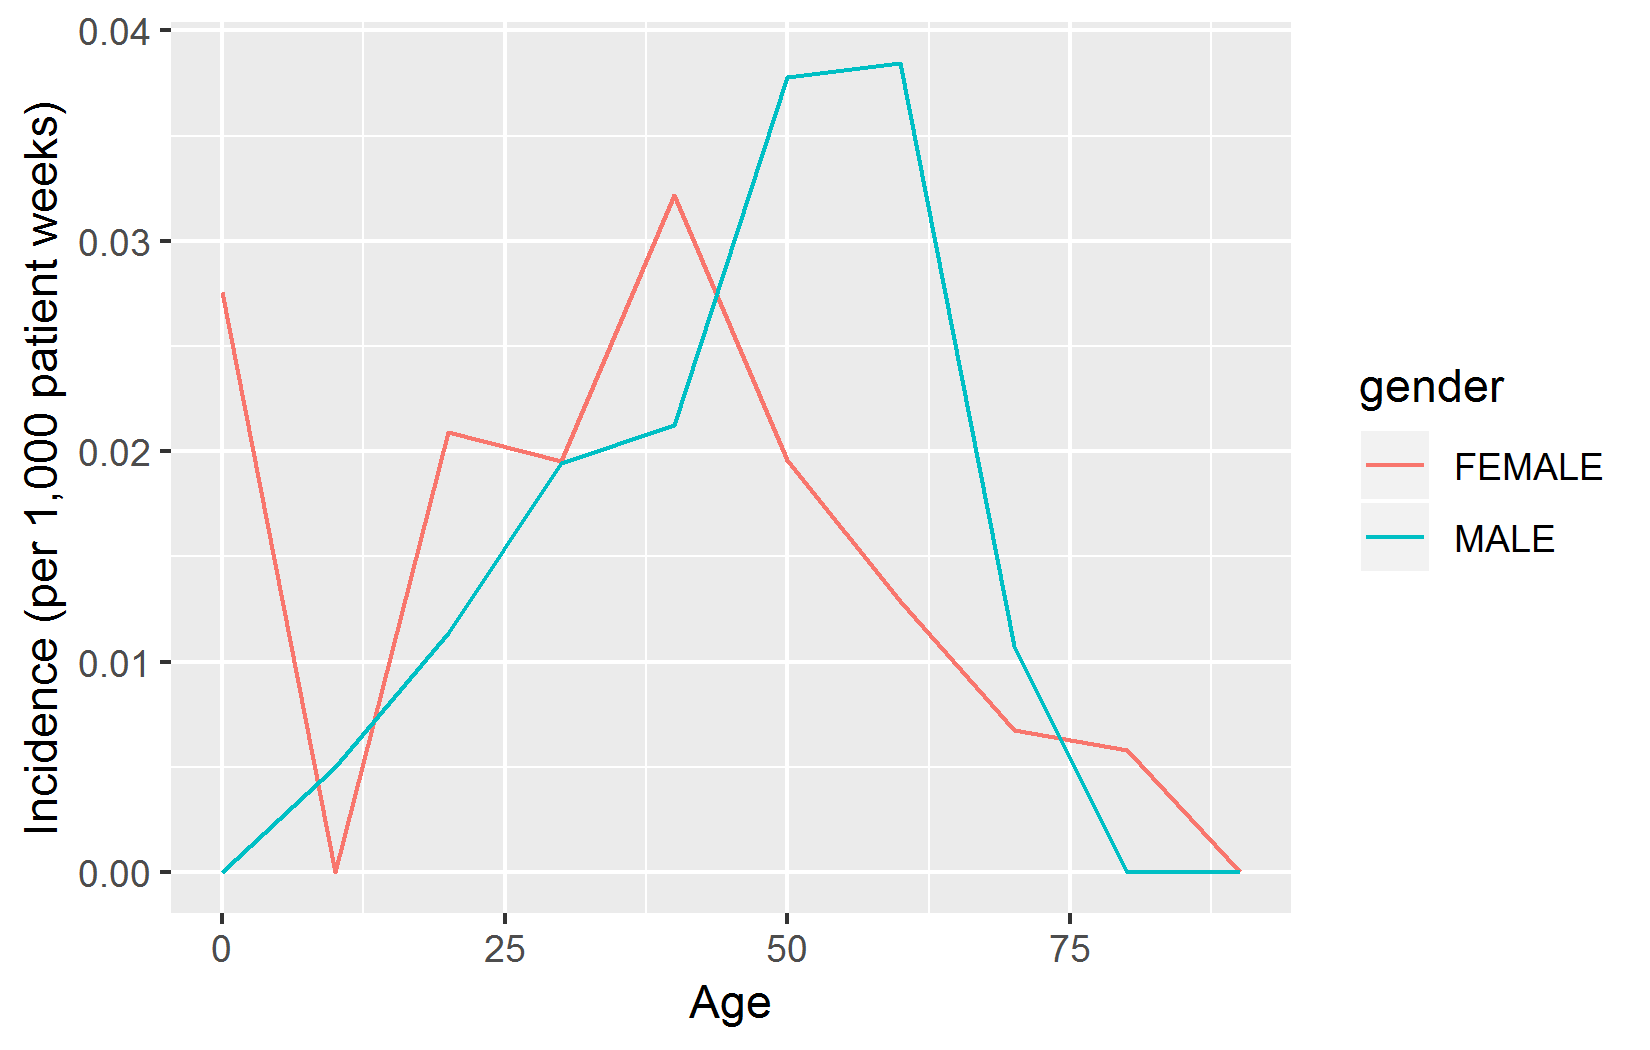
\includegraphics[width=0.8\linewidth]{images/SqlAndR/ir} \end{center}

\subsection{마무리하기}

생성한 테이블을 정리하고 연결을 닫는 것을 잊지 마십시오:

\begin{Shaded}
\begin{Highlighting}[]
\NormalTok{sql <-}\StringTok{ "}
\StringTok{TRUNCATE TABLE @cohort_db_schema.@cohort_table;}
\StringTok{DROP TABLE @cohort_db_schema.@cohort_table;}
\StringTok{"}
\KeywordTok{renderTranslateExecuteSql}\NormalTok{(conn, sql,}
                          \DataTypeTok{cohort_db_schema =}\NormalTok{ cohortDbSchema,}
                          \DataTypeTok{cohort_table =}\NormalTok{ cohortTable)}

\KeywordTok{disconnect}\NormalTok{(conn)}
\end{Highlighting}
\end{Shaded}

\subsection{호환성}

OHDSI SQL을 DatabaseConnector 및 SQLRender와 함께 사용하기 때문에 여기서
검토한 코드는 OHDSI가 지원하는 모든 데이터베이스 플랫폼에서 실행된다.

시연 목적으로 수작업으로 만든 SQL을 사용하여 코호트를 만들기로 했다는
점에 유의하십시오. ATLAS에서 코호트 정의를 구성하고 ATALS에서 생성된
SQL을 사용하여 코호트를 인스턴스화 하는 것이 더 편리했을 것이다. ATLAS는
또한 OHDSI SQL을 생성하였고, 따라서 SqlRender 및 DatabaseConnector와
함께 쉽게 사용할 수 있다.

\section{요약}\label{-7}

\BeginKnitrBlock{rmdsummary}
\begin{itemize}
\item
  \textbf{SQL}은 공통 데이터 모델을 따르는 데이터베이스를 포함하여
  데이터베이스를 조회하기 위한 표준 언어이다.
\item
  데이터베이스 플랫폼마다 SQL 언어가 다르며 이를 질의하기 위해서는 다른
  툴이 필요하다.
\item
  \textbf{SqlRender} 및 \textbf{DatabaseConnector} R 패키지는 CDM에서
  데이터를 질의하는 통합된 방법을 제공하므로 동일한 분석 코드를 수정없이
  다른 환경에서 실행할 수 있다.
\item
  R과 SQL을 함께 사용하면 OHDSI 툴에서 지원하지 않는 사용자 맞춤 분석
  연구를 구현할 수 있다.
\item
  \textbf{QueryLibrary} 는 CDM에 재사용 가능한 SQL 질의 모음을 제공한다.
\end{itemize}
\EndKnitrBlock{rmdsummary}

\section{예제}\label{-4}

\subsubsection*{전제조건}\label{-1}
\addcontentsline{toc}{subsubsection}{전제조건}

이 연습문제에서는 \ref{installR}절에서 설명된 대로 R, R-Studio, Java가
설치되었다고 가정한다. 또한 다음을 사용하여 설치할 수 있는
\href{https://ohdsi.github.io/SqlRender/}{SqlRender},
\href{https://ohdsi.github.io/DatabaseConnector/}{DatabaseConnector} 및
\href{https://ohdsi.github.io/Eunomia/}{Eunomia} 패키지도 필요하다:

\begin{Shaded}
\begin{Highlighting}[]
\KeywordTok{install.packages}\NormalTok{(}\KeywordTok{c}\NormalTok{(}\StringTok{"SqlRender"}\NormalTok{, }\StringTok{"DatabaseConnector"}\NormalTok{, }\StringTok{"devtools"}\NormalTok{))}
\NormalTok{devtools}\OperatorTok{::}\KeywordTok{install_github}\NormalTok{(}\StringTok{"ohdsi/Eunomia"}\NormalTok{, }\DataTypeTok{ref =} \StringTok{"v1.0.0"}\NormalTok{)}
\end{Highlighting}
\end{Shaded}

Eunomia 패키지는 로컬 R 세션 내에서 실행될 CDM의 시뮬레이션된 다른
데이터 세트를 제공한다. 연결 세부 사항은 다음을 사용하여 얻을 수 있다:

\begin{Shaded}
\begin{Highlighting}[]
\NormalTok{connectionDetails <-}\StringTok{ }\NormalTok{Eunomia}\OperatorTok{::}\KeywordTok{getEunomiaConnectionDetails}\NormalTok{()}
\end{Highlighting}
\end{Shaded}

CDM 데이터베이스 스키마는 ``main''이다.

\BeginKnitrBlock{exercise}
\protect\hypertarget{exr:exercisePeopleCount}{}{\label{exr:exercisePeopleCount}
}SQL과 R을 사용하여 데이터베이스에 몇 사람이 있는지 계산하십시오.
\EndKnitrBlock{exercise}

\BeginKnitrBlock{exercise}
\protect\hypertarget{exr:exerciseCelecoxibUsers}{}{\label{exr:exerciseCelecoxibUsers}
}SQL과 R을 사용하여 celecoxib를 적어도 한번 이상 처방 한 사람을
계산하십시오.
\EndKnitrBlock{exercise} \BeginKnitrBlock{exercise}

\protect\hypertarget{exr:exerciseGiBleedsDuringCelecoxib}{}{\label{exr:exerciseGiBleedsDuringCelecoxib}
}SQL과 R을 사용하여 celecoxib에 노출되는 동안 얼마나 많은 위장
출혈(gastrointestinal hemorrhage)이 있는지 진단한다. (힌트: 위장 출혈의
concept ID는
\href{http://athena.ohdsi.org/search-terms/terms/192671}{192671}이다.)
\EndKnitrBlock{exercise}

제안된 답변은 부록 \ref{SqlAndRanswers}에서 찾을 수 있다.

\chapter{코호트 만들기}\label{Cohorts}

\emph{Chapter lead: Kristin Kostka}

\emph{실세계 데이터(Real world data)}라고도 불리는 관찰 건강
정보(Observational health data)는 다양한 출처에서 꾸준하게 수집되는
환자의 건강 상태나 환자에게 제공되는 의료서비스에 관한 정보이다. CDM
데이터 유지를 위해 노력하는 OHDSI 공동 연구자들은 전자 의무기록,
보험청구자료, 결제 자료, 제품 및 질병 등록 정보 등을 포함하는 다양한
출처의 데이터를 활용하며, 환자 개인이 가정 내에서, 혹은 핸드폰 등의 다른
기기를 통해 생성한 건강 정보들을 활용하기도 한다. 이러한 데이터들은 연구
목적으로 수집된 데이터가 아니기 때문에 우리가 보고자 하는 임상 정보를
명료하게 담고 있지 못할 수도 있다.

예를 들어, 건강 보험 청구 자료 데이터베이스는 특정 질병 (예를 들어
혈관성부종)이 있는 환자에게 제공된 의료 서비스를 파악하고 그 치료비용을
의료기관에 상환해주기 위해 설립되었기 때문에, 상환목적에 맞는 정보만
부분적으로 담고 있다. 우리가 그런 데이터를 연구 목적으로 사용하기를
원한다면, 우리가 데이터를 사용할 때 실제로 관심 있는 것을 추론해야 하며,
타당한 추론을 가능케 하는 적절한 코호트를 설정해서 연구를 진행해야 한다.
그러므로 만약 우리가 보험 청구 자료 데이터베이스에서 새로 발생한 혈관성
부종만을 확인하고 싶다면, 코호트를 만들 때 이미 치료하고 있는 혈관성
부종 환자를 제외하기 위해서 응급실로 방문한 혈관성 부종 환자만을
코호트에 포함한다는 논리를 세워야 할 것이다. 전자 의무 기록에 담긴 임상
정보를 사용할 경우에도 비슷하다. 데이터를 이차적인 목적으로 사용하는
것이기 때문에 데이터베이스가 설립된 일차적인 목적을 인식하고 있어야
한다. 연구를 설계할 때마다 다양한 데이터베이스 환경에서 우리가 설정한
코호트가 어떻게 존재하고 있는지에 대한 뉘앙스를 항상 생각해야 한다.

이 장에서는 코호트를 생성하고 공유하는 것이 가지는 의미와 코호트를
개발하는 방법들, 그리고 ATLAS와 SQL을 이용해 당신만의 코호트를 생성하는
방법에 관해서 설명할 것이다.

\section{코호트란 무엇인가?}\label{-}

OHDSI 연구에서는 특정 기간 안에 하나 이상의 포함 기준에 속하는 사람들의
집단을 코호트라고 정의한다. 코호트는 때로 \emph{표현형(phenotype)}이라는
용어로 대신 사용하기도 한다. 코호트는 OHDSI 분석 도구를 사용하거나
연구를 시작하기 위한 첫 단계로 사용된다. 예를 들어 고혈압 치료약물인 ACE
inhibitor를 복용하기 시작한 사람 중에서 혈관성 부종이 일어날 위험을
예측하기 위한 연구를 진행할 때, 우리는 다음 두 가지 코호트를 지정해야
한다: 결과 코호트 (혈관성 부종이 발생한 사람들), 그리고 표적 코호트 (ACE
inhibitor를 복용하기 시작한 사람들). OHDSI에서 사용되는 코호트라는
개념이 가지는 중요한 특성은, 연구 내에서 지정된 각각의 코호트는 연구
내의 다른 코호트와 상호 비의존적이기 때문에 (그 연구만이 아닌 다른
연구에서도) 재사용이 가능하다는 것이다. 앞서 제시된 혈관성 부종 코호트를
예로 들어 보면, 이 코호트는 관찰되는 인구 내의 모든 혈관성 부종 발생
예를 담게 되며, 이는 표적 코호트에 포함되는 사람만이 아닌 그 외 다른
사람들도 포함될 수 있다는 것이다. 우리의 분석 툴은 두 코호트의 교집합을
분석할 것이다. 이것이 가지는 장점은, ACE inhibiter를 복용함으로써
발생하는 다른 결과를 분석할 때에도 이번에 만든 동일한 혈관성 부종
코호트를 재사용할 수 있다는 것이다.

\BeginKnitrBlock{rmdimportant}
코호트는 특정 시간 내에 하나 이상의 포함 기준을 만족시키는 사람들의
집합이다.
\EndKnitrBlock{rmdimportant}

\index{cohort} \index{cohort definition} OHDSI에서 사용되는 코호트의
정의가 다른 분야에서 사용되는 코호트의 정의와 다를 수 있다는 것을
인지하는 것이 중요하다. 예를 들어 제삼자 심사를 거친 많은 과학 논문에서,
코호트는 특정 임상 코드 집합 (예를 들어 ICD-9/ICD-10, NDC, HCPCS 등) 과
동일한 의미로 사용되었다. 하지만, 코드 집합들은 코호트를 설정하는 데
중요한 부분을 담당하지만, 코호트는 코드 집합에 의해서만 정의되는 것은
아니다. 코호트는 기준에 맞도록 코드 집합을 사용하는 특정 논리를 필요로
한다(예: 그 환자에게 첫 번째로 발생된 ICD-9/ICD-10 코드인가?). 잘 정의된
코호트는 환자가 어떻게 코호트에 포함되고 제외되는지를 구체적으로
설명한다. \index{code set}

\index{phenotype} OHDSI가 코호트를 정의하는 방식에는 다음과 같은 독특한
특징이 있다:

\begin{itemize}
\tightlist
\item
  한 사람은 여러 개의 코호트에 속할 수도 있다.
\item
  한 사람이 동일한 코호트 여러 다른 기간에 걸쳐 속할 수도 있다.
\item
  한 사람이 같은 기간에 동일한 코호트에 여러 번 속하지 않을 수도 있다
\item
  코호트에는 0명 혹은 그 이상의 구성원들을 가질 수도 있다.
\end{itemize}

코호트를 만드는 방법에는 두 가지 주요 방법이 있다:

\begin{enumerate}
\def\labelenumi{\arabic{enumi}.}
\tightlist
\item
  \textbf{규칙 기반 코호트 정의}는 언제 환자가 코호트 내에 속하는지에
  관한 명확한 포함 규칙을 가진다. 이 포함 규칙을 정하는 것은 코호트를
  디자인하는 사람들의 전문가적인 지식에 상당히 의존한다.
\item
  \textbf{확률적 코호트 정의}는 확률 모델을 사용하여 환자들이 코호트에
  속할 확률 (0\textasciitilde{}100\%) 을 계산한다. 이 확률은 역치 값을
  사용하여 `예-아니오' 분류로 전환할 수도 있고, 그대로 사용할 수도 있다.
  확률 모델은 일반적으로 예측 가능한 관련 환자 특성을 자동으로 식별하기
  위해 일부 기계학습모델 (예를 들어 로지스틱 회귀) 의 학습을 위해
  사용된다.
\end{enumerate}

다음으로 이 두 가지의 방법들에 대해서 구체적으로 알아보겠다.

\section{규칙 기반 코호트 정의}\label{---}

규칙 기반 코호트 정의는 특정 기간 내에 (예를 들어 ``지난 6개월 이내 해당
질병이 발생한 사람'') 하나 혹은 그 이상의 포함 기준 (예를 들어 ``혈관
부종을 앓는 환자들'') 을 명확히 제시함으로써 시작한다.
\index{cohort!rule-based design}

이러한 기준을 만드는 데 사용되는 표준 구성 요소는 다음과 같다:

\begin{itemize}
\item
  \textbf{도메인}: CDM 도메인 (예를 들어 ``Procedure Occurrence'',
  ``Drug Exposure'')은 데이터가 저장되는 곳인데, 도메인의 종류에 따라
  어떤 유형의 임상 정보가 담길지, 어떤 개념들이 담길지가 결정된다.
  도메인에 관한 세부사항은 \ref{domains}절에서 확인할 수 있다.
\item
  \textbf{개념 모음(Concept set)}: 우리가 관심을 가지는 임상적 개념을
  대변하는 하나 이상의 표준화된 개념의 모음을 의미한다. 개념 모음은 표준
  용어들 (임상에서 쓰이는 용어들은 국가나 병원, 사람에 따라 동일한
  개념도 조금씩 다른 용어로 사용되는데 이를 표준 용어로 매핑함) 로
  구성되어 있기 때문에 다양한 관찰 의료 데이터에서 상호 운용이 가능하다.
  Concept set에 관하여 \ref{conceptSets}절에 자세한 설명이 있다.
\item
  \textbf{도메인별 속성}: 관심 있는 임상 실체와 연관된 추가적인 속성들
  (예를 들어 DRUG\_EXPOSURE의 DAYS\_SUPPLY, MEASUREMENT의
  VALUE\_AS\_NUMBER와 RANGE\_HIGH)
\item
  \textbf{시간의 설정}: 선정 기준과 임상사건 발생 간의 시간 간격 (예를
  들어 노출 시작 또는 노출 시작 후 365일 이내에 특정 조건이 발생해야 함)
\end{itemize}

코호트 정의를 작성할 때, 코호트 속성을 나타내는 도메인을 빌딩 블록 (그림
\ref{fig:cohortLegos} 참조) 과 유사하게 생각하면 도움이 될 수 있다. 각
도메인에서 허용 가능한 구성 요소에 대해 혼란스럽다면 언제든지 공통
데이터 모델 \ref{CommonDataModel}장을 참조하라.

\begin{figure}

{\centering 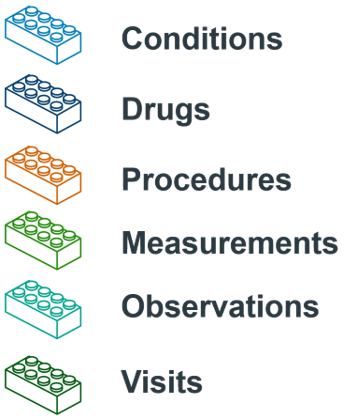
\includegraphics[width=0.5\linewidth]{images/Cohorts/cohort-legos} 

}

\caption{코호트 정의를 위한 빌딩 블록}\label{fig:cohortLegos}
\end{figure}

코호트 정의를 작성할 때, 다음과 같은 질문에 답할 수 있어야 한다:

\begin{itemize}
\tightlist
\item
  \emph{코호트 진입 시간을 정의하는 초기 이벤트는 무엇인가?}
\item
  \emph{초기 이벤트에는 어떤 포함 기준이 적용되는가?}
\item
  \emph{코호트 종료 시간을 정의하는 것은 무엇인가?}
\end{itemize}

\textbf{코호트 진입 이벤트}: 코호트 진입 이벤트(초기 이벤트)는 사람들이
코호트에 진입하는 \textbf{코호트 기준시점(cohort index date)} 으로
정의된다. 코호트 진입 이벤트는 약물 노출(Drug exposure), 질병
상태(conditions), 절차(procedures), 측정(measurements) 및 방문(visits)과
같은 CDM에 기록된 모든 사건일 수 있다. 초기 이벤트는 데이터가 저장되는
CDM 도메인(예를 들어 PROCEDURS\_OCCURRENCE, DRUG\_EXPOSURE 등), 임상
활동을 식별하기 위해 구축된 개념 모음 (예를 들어 질병 상태에 대한 SNOMED
코드, 약물에 대한 RxNorm 코드) 및 기타 특정 속성들 (예를 들어 발생 연령,
첫 진단 / 절차 등, 지정된 시작 및 종료 날짜, 방문 유형 등) 에 의해
정의된다. 진입 이벤트를 가진 사람들의 집합을 \textbf{초기 사건 코호트
initial event cohort} 라고 한다. \index{cohort!entry event}

\textbf{포함 기준}: 포함 기준은 초기 이벤트 코호트에 적용되어 코호트에
진입할 사람들을 추가로 제한한다. 각 포함 기준을 만들 때는 데이터가
저장되는 CDM 도메인, 컨셉 모음, 도메인별 속성 (예를 들어 days supply,
방문 유형) 및 코호트 색인 날짜에 관한 시간 논리를 결정해야 한다.
\textbf{적격 코호트(qualifying cohort)}는 초기 이벤트 코호트에서 모든
포함 기준을 충족하는 사람들의 집합으로 정의한다.
\index{cohort!inclusion criteria}

\textbf{코호트 종료 기준}: 코호트 종료 이벤트는 한 사람이 더 이상 코호트
자격 요건을 갖추지 못했을 때를 의미한다. 코호트 종료는 관찰 기간이
끝났을 때, 초기 진입 이벤트로부터 일정한 시간이 지났을 때 혹은 마지막
이벤트가 발생했을 때 등 여러 방법으로 정의할 수 있다. 코호트 종료 기준에
따라 한 사람의 오랜 시간에 걸친 기록 중에서 특정한 기간이 선정기준에
맞아 코호트에 한 번 포함된 후에 또 다른 기간이 코호트 선정 기간에 맞아
다시 코호트에 포함되는 등 한 사람의 관찰이 하나의 코호트에 여러 번 속할
수 있다.\index{cohort!exit criteria}

\BeginKnitrBlock{rmdimportant}
OHDSI 도구에는 포함 기준과 제외 기준이 구분되지 않는다. 모든 기준은 포함
기준으로 설정해야 한다. 예를 들어 `사전 고혈압 환자 제외'라는 제외
기준을 `사전 고혈압 발생이 0인 사람들 포함'이라는 포함 기준으로 설정해야
한다.
\EndKnitrBlock{rmdimportant}

\section{개념 모음}\label{conceptSets}

\index{concept set}

개념 모음을 구성하는 개념들은 다양한 다른 분석들에서 재사용이 가능하다.
개념 모음은 관찰 연구들에서 종종 사용되는 표준화된 컴퓨터 코드라고
생각해도 된다. 개념 모음은 다음 특성들을 포함하고 있다:

\begin{itemize}
\tightlist
\item
  \textbf{Exclude}: 개념 모음으로부터 해당 개념과 해당 개념의 하위
  개념들을 제외하라.
\item
  \textbf{Descendants}: 이 개념뿐만 아니라 모든 하위 항목 개념들을
  고려하라.
\item
  \textbf{Mapped}: 표준화되지 않은 개념들도 검색하라.
\end{itemize}

예를 들어 표 \ref{tab:conceptSetExpression}과 같이 개념 모음은 두 개의
개념들을 포함할 수 있다. 여기서 우리는
\href{http://athena.ohdsi.org/search-terms/terms/4329847}{4329847}
(``심근경색 Myocardial infarction'') 과 그 모든 하위 개념들을 포함했고,
\href{http://athena.ohdsi.org/search-terms/terms/314666}{314666}
(``과거심근경색 Old myocardial infarction'') 과 그 모든 하위 개념들은
제외했다.

\begin{longtable}[]{@{}lllll@{}}
\caption{\label{tab:conceptSetExpression} 개념 모음의 예시}\tabularnewline
\toprule
Concept Id & Concept Name & Excluded & Descendants &
Mapped\tabularnewline
\midrule
\endfirsthead
\toprule
Concept Id & Concept Name & Excluded & Descendants &
Mapped\tabularnewline
\midrule
\endhead
4329847 & Myocardial infarction & NO & YES & NO\tabularnewline
314666 & Old myocardial infarction & YES & YES & NO\tabularnewline
\bottomrule
\end{longtable}

그림 \ref{fig:conceptSet}에서 볼 수 있다시피, ``심근경색 Myocardial
infarction'' 과 그 모든 하위 개념들을 포함할 것이고, 하위 개념 중에서
``과거 심근경색 Old myocardial infarction'' 와 그 모든 하위 개념들은
제외할 것이다. 결과적으로 거의 100개 정도의 표준 개념들을 포함한 개념
모음이 만들어졌다. 이 표준 개념들은 다양한 데이터베이스에서 사용되는
수백 개의 소스 코드 (예를 들어 ICD-9, ICD-10) 를 반영한다.

\begin{figure}

{\centering 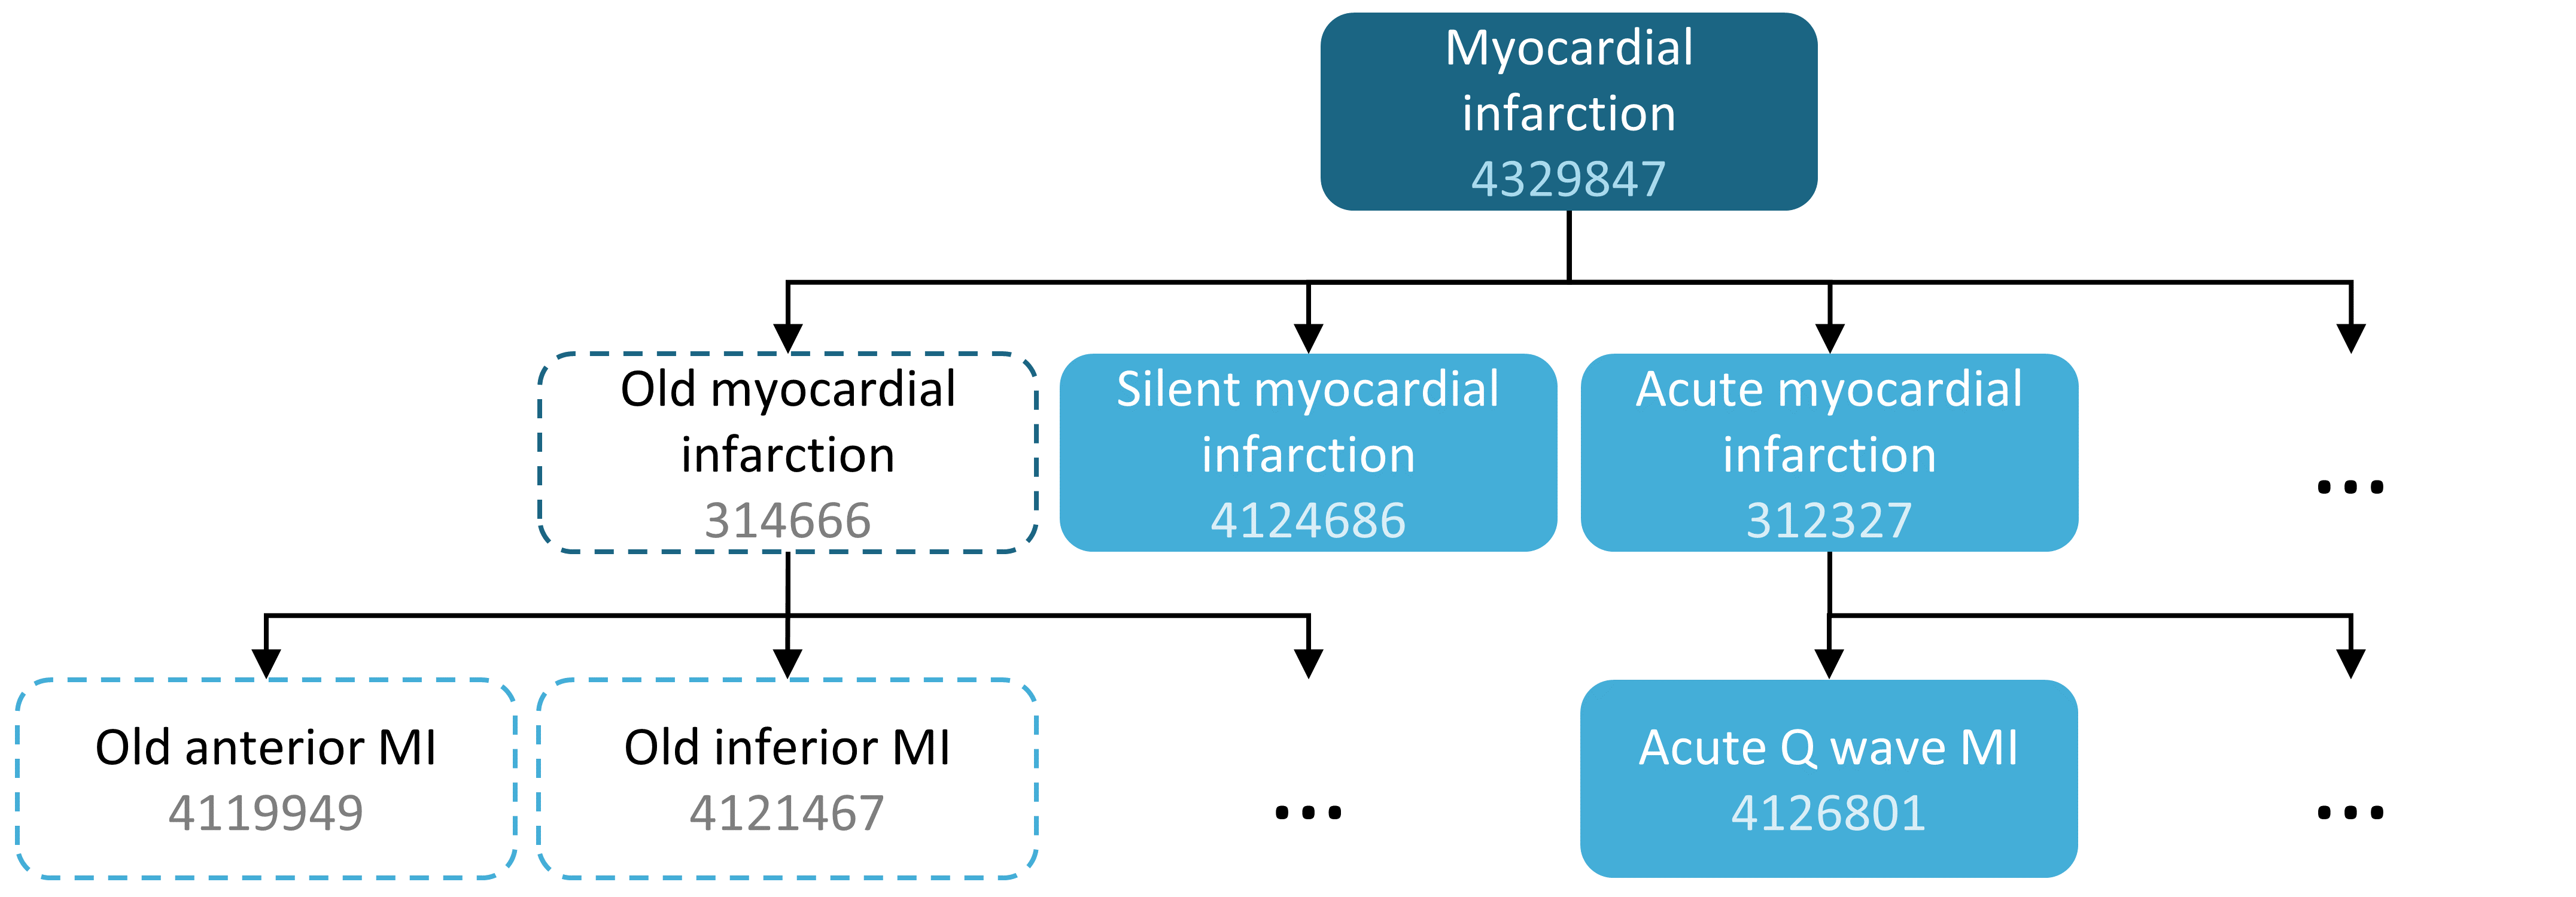
\includegraphics[width=1\linewidth]{images/Cohorts/conceptSet} 

}

\caption{"Myocardial infaction"와 그 하위 개념을 포함하지만 "Old myocardial infarction"과 그 하위 개념은 제외하는 개념 모음}\label{fig:conceptSet}
\end{figure}

\section{확률적 코호트 정의}\label{--}

규칙 기반 코호트 정의는 코호트 정의를 수행할 때 널리 사용되는 방법이다.
그러나 코호트를 만들기 위해 전문가끼리 합의를 이루는 것은 매우 많은
시간이 소요되는 일이다. 확률적 코호트 정의는 코호트 속성의 효율적인
선택을 위한 대안적인 기계 구동 방식이다. 이 접근법에서, 지도 기계학습은
코호트를 설계하는 알고리즘이 레이블이 붙은 증례로부터 학습할 수 있게
한다. 이 알고리즘은 더 나은 코호트 설계를 위해 사용될 것이다.
\index{cohort!probabilistic design}

이 접근 방법을 CDM의 데이터에 적용한 예는 아프로디테(APHRODITE:
Automated PHenotype Routine for Observational Definition,
Identification, Training and Evaluation) R 패키지이다. 이 패키지는
불완전하게 레이블이 붙은 데이터로부터 학습하는 능력을 결합한 코호트 구축
프레임워크를 제공한다. \citep{Banda2017APHRODITE} \index{APHRODITE}

\section{코호트 정의 유효성}\label{--}

코호트를 구축할 때, 다음 중 더 중요한 것이 무엇인지 고려하는 것이
필요하다: \emph{코호트 조건에 해당하는 환자를 모두 찾는 것이 더
중요한가? 아니면 확신이 가는 환자들만 찾는 것이 더 중요한가?}

코호트를 구축할 때 당신의 전략은 전문가가 질병을 얼마나 엄격하게
정의하는지에 의존할 것이다. 얻을 수 있는 모든 것을 사용하거나, 최소
공통분모를 사용하거나 이 둘을 절충하는 코호트 정의를 작성할 수 있다.
관심 코호트를 적절하게 연구하기 위해 얼마나 엄격한 임계값을 사용할지는
궁극적으로 연구자의 재량에 달려 있다.

이 장의 시작 부분에서 언급했듯이 코호트 정의는 데이터로부터 무엇인가
관찰하고자 하는 것을 유추하려는 시도이다. 그러면 그러한 시도에서
코호트를 얼마나 잘 정의했는지 의문을 품게 된다. 일반적으로, 규칙 기반의
코호트 정의나 확률적 알고리즘의 검증은 작성한 코호트를 `절대 표준 gold
standard' 참고 값 (즉 수작업으로 챠트리뷰한 것)과 비교함으로써 검증할 수
있다. 이에 대해서는 \ref{ClinicalValidity}장(``임상적 타당성'') 에서
자세히 설명한다.

\subsection{OHDSI 절대 표준 표현형 라이브러리}\label{ohdsi----}

커뮤니티를 지원하기 위해서 OHDSI 절대 표준 표현형 라이브러리(OHDSI Gold
Standard Phenotype Library, GSPL) 그룹이 형성되었다. GSPL 그룹의 목표는
규칙 기반 및 확률적 방법으로 커뮤니티 기반의 코호트 라이브러리를
개발하는 것이다. GSPL은 OHDSI 커뮤니티의 멤버들이 각자의 연구를 위해
커뮤니티가 검증한 코호트를 찾아서 실행시킬 수 있게 하였다. 이 `절대
표준(gold standard)' 코호트들은 라이브러리 안에 들어 있다. GSPL과 관련된
추가적인 정보를 얻으려면 OHDSI work group 페이지에 문의하라. 이전에
소개되었던 APHRODITE \citep{Banda2017APHRODITE} 와 PheValuator tool
\citep{Swerdel2019phevaluator} 뿐만 아니라 OHDSI 네트워크에서 전자 의무
기록과 유전 정보를 공유하기 위해 만들어진 eMERGE Phenotype Library
\href{https://emerge.mc.vanderbilt.edu/}{eMERGE}
\href{https://phekb.org/phenotypes}{Phenotype Library}
\citep{Hripcsak2019eMERGE} 도 해당 작업 그룹에서 다루고 있다. 당신이
코호트를 설계하는 데 관심이 많다면, 이 작업 그룹에 참여해 보라.
\index{phenotype library}

\section{고혈압 환자 코호트 작성하기}\label{---}

규칙 기반의 접근 방법으로 코호트를 작성해보자. 이번 예제에서는,
\emph{고혈압의 초기 치료를 위해 ACE inhibitors 단일 치료를 시작한
환자}를 찾을 것이다.

이 연습을 진행하면서 표준 감소 차트와 비슷한 코호트를 작성하게 될
것이다. 그림 \ref{fig:CohortPractice}은 우리가 어떤 논리로 코호트를
작성할지 보여준다.

\begin{figure}

{\centering 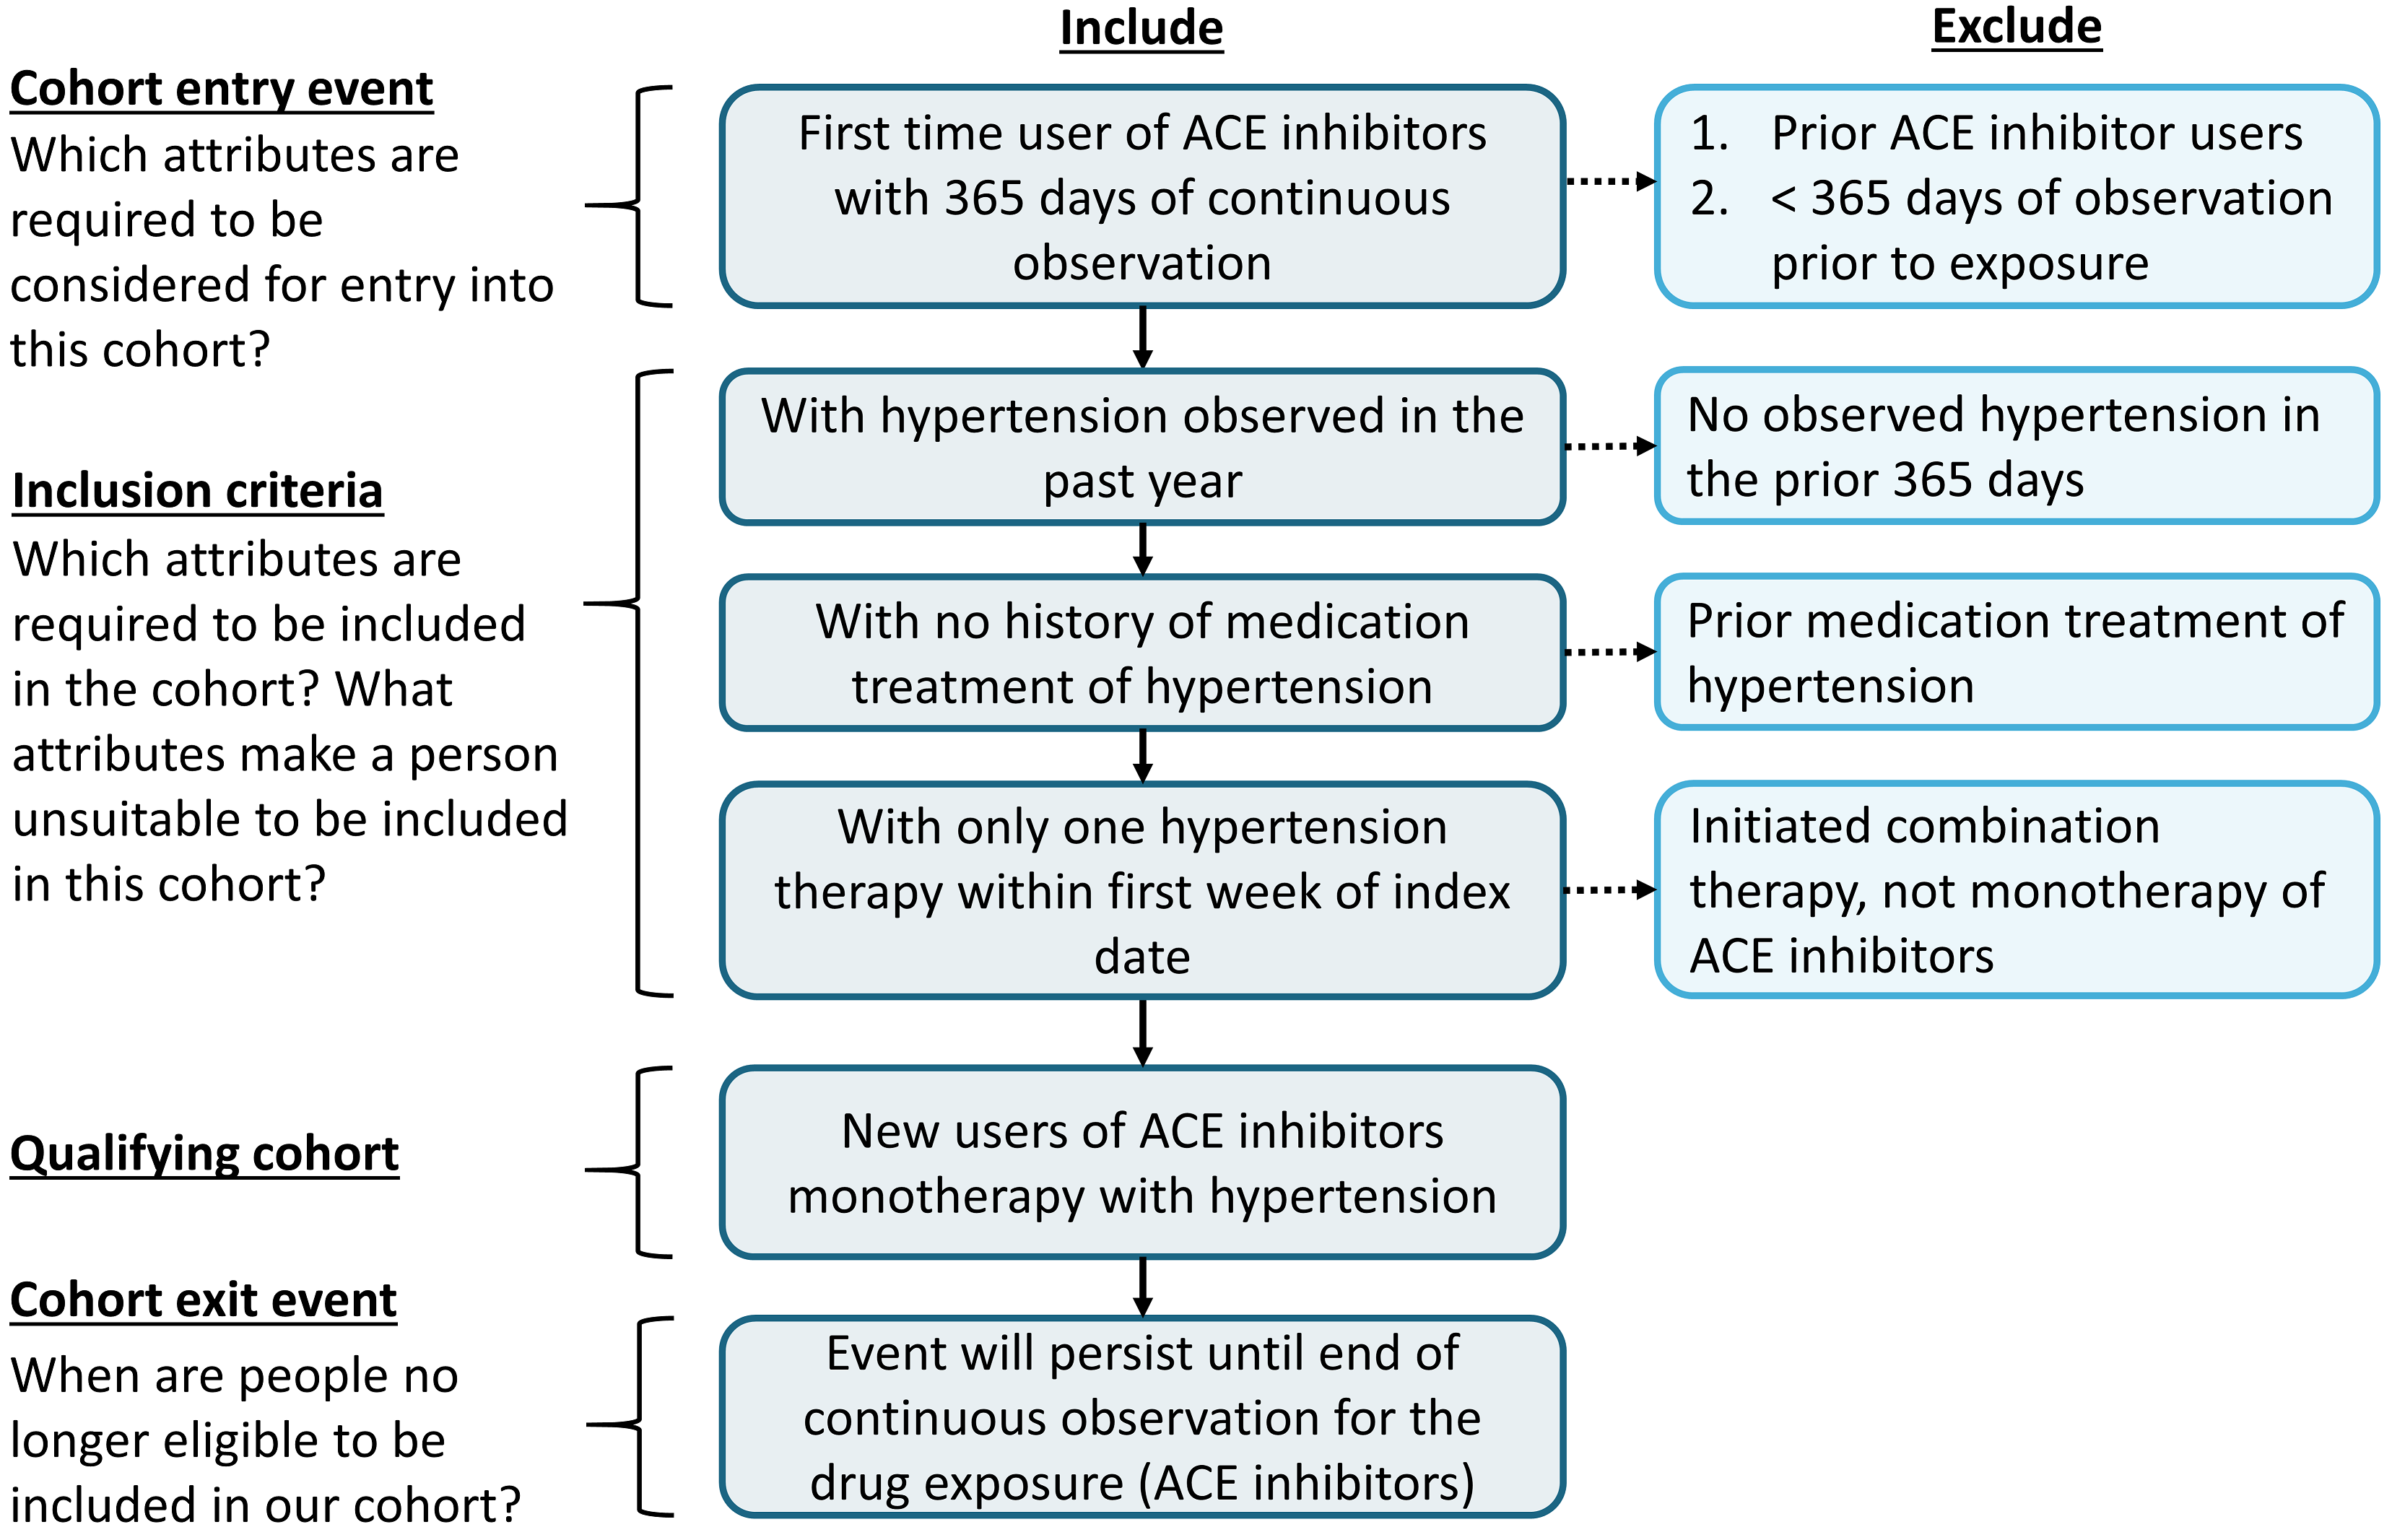
\includegraphics[width=1\linewidth]{images/Cohorts/CohortPractice} 

}

\caption{만들고자 하는 코호트의 논리적 구성도}\label{fig:CohortPractice}
\end{figure}

ATLAS 유저 인터페이스를 사용해서 코호트를 작성해도 되고, 쿼리를 직접
작성해도 된다. 이 장에서는 두 가지 방법 모두에 대해 간단히 소개하겠다.

\section{ATLAS를 이용해 코호트 작성하기}\label{atlas---}

ATLAS를 시작하기 위해

\includegraphics{images/Cohorts/cohortdefinition.png} 버튼을 클릭하라.
다음으로 `New cohort' 버튼을 클릭하라. 다음 화면에서 비어 있는 코호트를
확인할 수 있을 것이다. 그림 \ref{fig:ATLASdefineacohort}에서 당신이 현재
보고 있는 화면을 확인하라.

\begin{figure}

{\centering 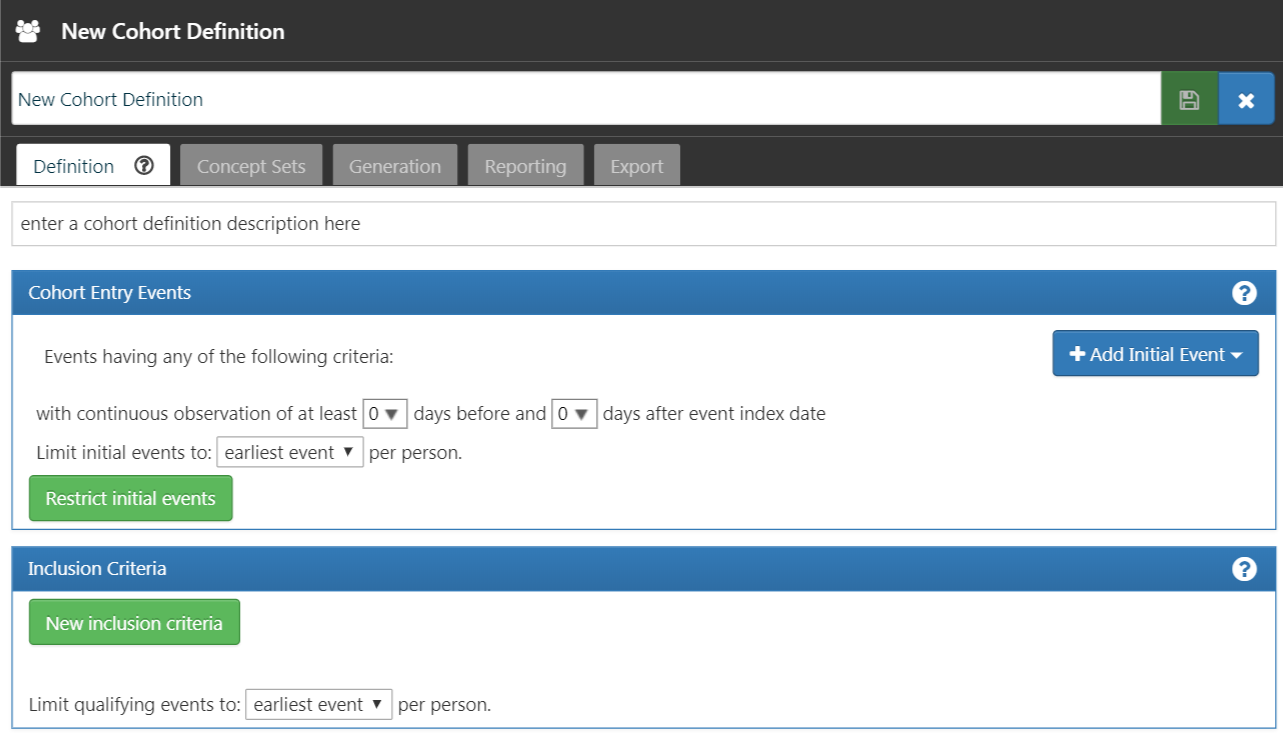
\includegraphics[width=1\linewidth]{images/Cohorts/ATLAS-defineacohort} 

}

\caption{새로운 코호트 정의}\label{fig:ATLASdefineacohort}
\end{figure}

먼저 ``New Cohort Definition''로 지정되어 있는 코호트 이름을 다른
이름으로 바꿔 지어 주기를 추천한다. 'New users of ACE inhibitors as
first-line monotherapy for hypertension'라고 지으면 적당할 것이다.

\BeginKnitrBlock{rmdimportant}
ATLAS는 동일한 이름을 가진 두 개의 코호트가 존재하는 것을 허락하지
않는다. 기존에 있던 이름을 사용하려고 하면 에러 메시지가 뜰 것이다.
\EndKnitrBlock{rmdimportant}

이름을 정했으면, 
\includegraphics{images/Cohorts/save.png}을 눌러서
코호트를 저장하십시오.

\subsection{초기 이벤트 기준}\label{--}

이제 우리는 초기 코호트 이벤트를 정의해야 한다. ``Add initial event''를
클릭하라. 어떤 도메인 내에서 기준을 설정할지 결정해야 한다. 초기 코호트
이벤트를 정의하기 위해 어떤 도메인이 필요한지 어떻게 알 수 있을까? 함께
알아보자.

\begin{figure}

{\centering 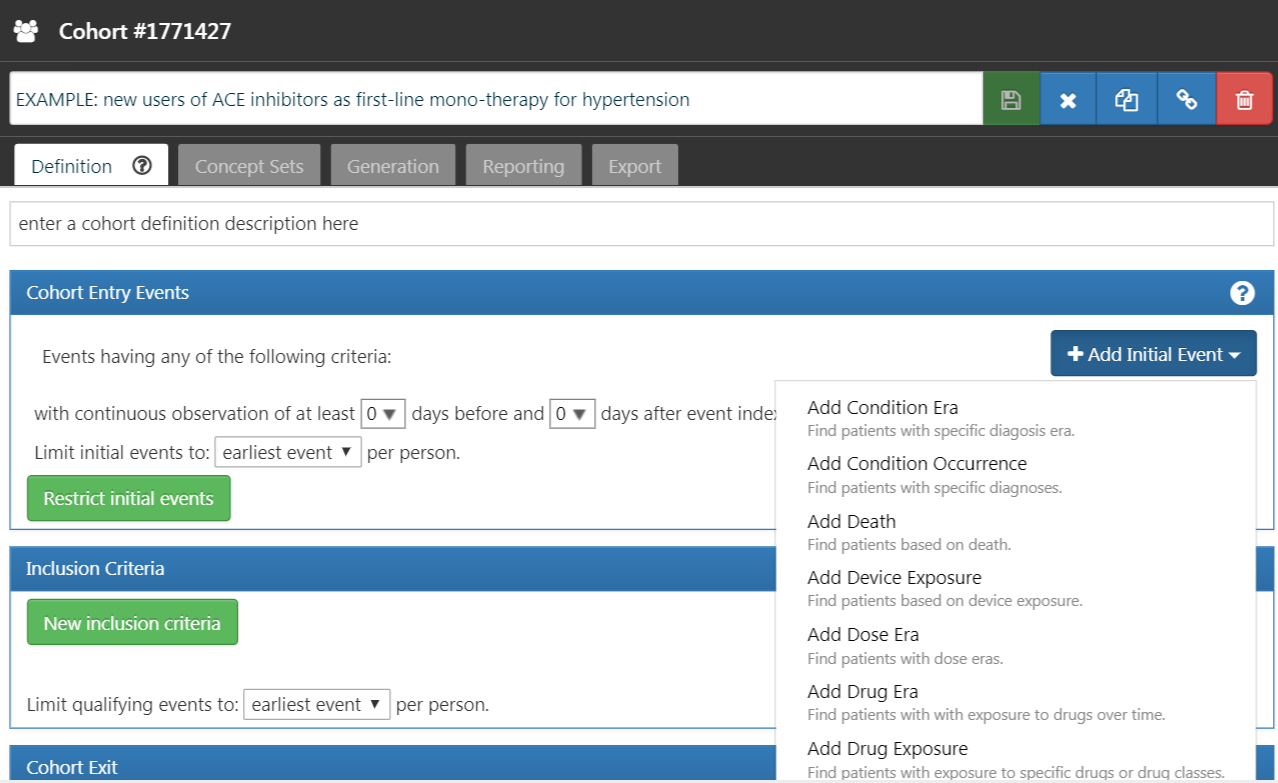
\includegraphics[width=1\linewidth]{images/Cohorts/ATLAS-initialevent} 

}

\caption{초기 이벤트 추가하기}\label{fig:ATLASinitialevent}
\end{figure}

그림 \ref{fig:ATLASinitialevent}에서 볼 수 있듯이 ATLAS는 각 기준들
아래에 설명을 제공한다. 우리가 만약 특정 질병을 진단받은 환자들을 찾으려
한다면 CONDITION\_OCCURRENCE 도메인에서 기준을 만들어야 한다. 특정
약물이나 특정 계열의 약물을 복용한 환자를 찾고 싶다면 DRUG\_EXPOSURE
도메인에서 기준을 만들어야 한다. 우리는 고혈압의 초치료로 ACE inhibitors
단독요법을 시행한 환자들을 찾고 싶기 때문에 DRUG\_EXPOSURE 도메인에서
기준을 만들어야 한다. 그런데 고혈압을 진단받은 환자도 찾아야 하지
않는가? 맞다! 고혈압 진단과 관련해서는 다른 기준을 만들 것이다. 하지만
고혈압 약물을 복용하기 시작한 날짜가 코호트 시작 날짜, 즉 시작 이벤트가
될 것이다. 고혈압 진단은 소위 \emph{추가적 적격 기준(additional
qualifying criteria)}이 된다. 이에 관해서는 뒤에서 다시 설명하겠다. 이제
'Add Drug Exposure'를 클릭하라.

화면은 당신이 선택한 기준에 따라 업데이트되겠지만, 아직 끝난 것은
아니다. 그림 \ref{fig:ATLASdrugexposure}에서 볼 수 있다시피 ATLAS는
우리가 어떤 약물을 찾고자 하는지 아직 모른다. ATLAS에게 어떤 개념 모음이
ACE inhibitors와 연관이 있는지 알려주어야 한다.

\begin{figure}

{\centering \includegraphics[width=1\linewidth]{images/Cohorts/ATLAS-drugexposure} 

}

\caption{약물 복용에 관하여 정의하기}\label{fig:ATLASdrugexposure}
\end{figure}

\subsection{개념 모음 정의하기}\label{--}

ACE inhibitors를 정의하기 위한 대화 상자를 열기 위해
\includegraphics{images/Cohorts/downarrow.png}을 클릭하라.

\subsubsection*{시나리오 1: 당신은 아직 개념 모음을 만들지
않았다}\label{-1------}
\addcontentsline{toc}{subsubsection}{시나리오 1: 당신은 아직 개념 모음을
만들지 않았다}

아직 당신의 코호트에 추가할 개념 모음을 만들지 않았다면, 이것을 먼저
진행해야 한다. `Concept set' 탭의 'New Concept Set'을 클릭하여 코호트를
작성하는 데 쓰일 개념 모음을 만들 수 있다. 개념 모음의 이름을 'Unnamed
Concept Set'에서 새로 만들어 주어야 한다. 이제
\includegraphics{images/Cohorts/search-2.png} 모듈을 통해 ACE
inhibitors를 나타내는 개념을 찾아보자. (그림 \ref{fig:aceinhibitors})

\begin{figure}

{\centering \includegraphics[width=1\linewidth]{images/Cohorts/aceinhibitors} 

}

\caption{ACE Inhibitors 용어 찾기}\label{fig:aceinhibitors}
\end{figure}

필요한 용어들을 찾았다면,
\includegraphics{images/Cohorts/shoppingcart.png}을 클릭함으로써 그
개념을 선택할 수 있다. 그림 \ref{fig:aceinhibitors}의 좌상단의 왼쪽을
향하는 화살표 버튼을 클릭하여 코호트 작성 페이지로 돌아갈 수 있다.
적절한 용어를 찾기 위한 방법은 \ref{StandardizedVocabularies}장(``표준
용어'')을 참고하라.

그림 \ref{fig:aceConceptSetExpression}에서 우리가 선택한 개념 모음의
구성을 확인할 수 있다. 우리는 모든 ACE inhibitors 성분들을 선택했으며,
그것들의 하위 개념들도 포함시켰다. 'Included concepts'를 클릭하여 포함된
21,536개의 모든 개념을 확인할 수 있고, 'Included Source Codes'를
클릭하여 모든 소스 코드들을 확인할 수도 있다.

\begin{figure}

{\centering \includegraphics[width=1\linewidth]{images/Cohorts/aceConceptSetExpression} 

}

\caption{ACE inhibitor를 포함한 약물들의 개념 모음}\label{fig:aceConceptSetExpression}
\end{figure}

\subsubsection*{시나리오 2: 당신은 이미 개념 모음을
만들었다}\label{-2-----}
\addcontentsline{toc}{subsubsection}{시나리오 2: 당신은 이미 개념 모음을
만들었다}

만약 당신이 이미 개념 모음을 만들었고, ATLAS에 저장했다면, 'Import
Concept Set'을 클릭하라. 그러면 그림 \ref{fig:ATLASfindyourconcept}에서
볼 수 있다시피 ATLAS의 개념 모음 저장소에서 당신의 개념 모음을 찾을 수
있는 대화창이 뜬다. 이번 예시에서는 사용자가 ATLAS에 저장되어 있던 개념
모음을 이용한다고 가정하자. 사용자는 검색 창에 'ACE inhibitors'를
검색하였고, 검색 내용이 이름에 포함된 개념 모음들을 볼 수 있을 것이다.
사용자는 해당하는 개념 모음을 클릭하여 선택할 수 있다 (참고로 당신이
개념 모음을 선택하면 대화창은 사라진다). Any Drug 칸이 당신이 선택한
개념 모음의 이름으로 바뀌어 있다면 성공한 것이다.

\begin{figure}

{\centering \includegraphics[width=1\linewidth]{images/Cohorts/ATLAS-findingyourconcept} 

}

\caption{ATLAS 저장소에서 개념 모음을 가져오기}\label{fig:ATLASfindyourconcept}
\end{figure}

\subsection{추가적 초기 이벤트 기준}\label{---}

이제 코호트에 개념 모음을 만들어 붙였지만, 아직 끝난 것이 아니다. 우리는
ACE inhibitors를 태어나서 처음 복용한 사람들을 찾고 있다. 이는 ACE
inhibitors을 처음 복용한 환자 기록을 찾는 것을 의미한다. 이를 지정하기
위해 당신은 '+Add attribute'를 클릭하여 'Add first exposure criteria'를
선택해야 한다. 당신이 만든 기준에 다른 특성들도 지정할 수 있다는 것을
참고하라. 약물을 복용한 날짜나 나이, 성별 혹은 약물과 관련한 다른
특성들을 지정할 수 있다. 각 도메인에 따라 선택할 수 있는 특성들이
다르다.

선택을 했으면, 창은 자동으로 닫힌다. 선택된 특성은 초기 기준과 같은 칸
안에서 볼 수 있을 것이다 (그림 \ref{fig:initialEventAce} 참조).

\BeginKnitrBlock{rmdimportant}
현재 ATLAS 디자인은 활용하기에 약간 혼란스러울 수 있다. 생긴 모양과는
다르게 버튼 \includegraphics{images/Cohorts/redX.png}는 'NO'를 의미하는
것이 아니다. 이는 사용자에게 해당 기준을 삭제할 수 있도록 만들어진
버튼이다. 만약 당신이 \includegraphics{images/Cohorts/redX.png}를
클릭한다면, 해당 기준은 사라질 것이다. 그러므로 당신의 기준을 사라지지
않은 채 그대로 보존시키고 싶다면, 옆에
\includegraphics{images/Cohorts/redX.png} 버튼을 그대로 놔두어야 한다.
\EndKnitrBlock{rmdimportant}

이제 만족스러운 초기 이벤트를 설정했다. 환자가 처음으로 약물을
복용했다는 사실을 보증하기 위해, 환자의 그 이전 기록을 확인할 수 있는
충분한 기간을 설정해 주면 좋을 것이다. 짧은 관찰 기간을 가진 환자들은
우리가 확인할 수 없는 다른 곳에서 약물을 복용하였을 수도 있다. 우리가
이것을 강제적으로 막을 수는 없지만 기준일자 index date 이전에 관찰
기간을 설정함으로써 최소한 해당 관찰 기간 동안에는 약물 복용이
이루어지지 않았음을 보증할 수 있다. 이를 위해 관찰 기간을 설정하는
부분이 있으며, 구체적인 관찰 기간을 직접 설정할 수도 있다. 우리는 초기
이벤트 이전에 365일 동안 관찰된 환자를 필요로 한다. 그림
\ref{fig:initialEventAce}처럼 관찰 기간을 다음과 같이 설정하라:
\emph{with continuous observation of 365 days before.} 당신 연구 팀의
재량껏 관찰 기간을 설정하면 된다. 다른 코호트에서는 관찰 기간을 다르게
설정해서 다양한 시도들을 해볼 수 있다. 이는 환자의 과거력에 관한
기간이며, 기준일자 index date 이후의 시간은 포함하지 않는다. 그러므로
우리는 0 dates after index date라고 설정해야 한다. 우리는 생에 처음 ACE
inhibitors를 복용한 환자를 찾고 싶기 때문에 \emph{limit initial events
to the ``earliest event'' per person} (한 환자에서 발생한 여러 번의 ACE
inhibitor 복용 중, 첫 번째 복용을 초기 이벤트로 설정하는 것) 으로
설정한다.

\begin{figure}

{\centering \includegraphics[width=1\linewidth]{images/Cohorts/initialEventAce} 

}

\caption{Index date 이전에 필요로 하는 관찰 기간 설정하기.}\label{fig:initialEventAce}
\end{figure}

지금껏 설정한 논리를 한 눈에 보기 위해서 환자의 타임라인을 설정해볼 수
있다.

\begin{figure}

{\centering \includegraphics[width=1\linewidth]{images/Cohorts/EarliestEventExplained} 

}

\caption{기준들이 적용됨에 따라 환자가 코호트에 적합한지 살펴보기}\label{fig:EarliestEventExplained}
\end{figure}

그림 \ref{fig:EarliestEventExplained}에서 각 행은 코호트에 들어올 자격을
갖출 수 있는 환자 개개인을 나타낸다. 그리고 진한 별들은 환자가 특정
기준을 만족했던 시간을 나타낸다. 추가 기준이 설정될수록 진한 별들 대신
연한 별들이 그려진 것을 볼 수 있다 (즉, 추가 기준에 의해서 코호트에
포함되지 못하고 탈락). 이는 환자가 조건들을 모두 만족하는 이벤트도
가지고 있지만, 그렇지 않은 이벤트도 가지고 있음을 의미한다. 마지막
기준을 그린 그림을 보면 ACE inhibitors를 처음으로 복용하였으며, 복용
이전에 최소 365일의 관찰 기간을 가진 환자 (환자 1번, 환자 3번, 환자
5번의 진한 별은 관찰에 포함; 환자 1번의 연한 별은 관찰에서 탈락)들을
확인할 수 있다. 당신의 코호트를 설계할 때
\href{http://forums.ohdsi.org}{OHDSI Forum}에 참여하는 연구자들의 의견을
참고하면 더 좋을 것이다.

\subsection{포함 기준}\label{-}

코호트 진입 이벤트를 설정했으면, 다음 두 옵션을 통해 추가적 이벤트를
설정할 수 있다: `Restrict initial events', 그리고 `New inclusion
criteria'. 이 두 옵션 사이에는 ATLAS가 사용자에게 어떤 임시 정보를
제공하는가의 차이가 있다. 만약 당신이 기준을 추가하기 위해 'Restrict
initial events'를 사용한다면, ATLAS에서 조건에 맞는 대상 환자 수를 셀
때, 모든 기준들을 충족시키는 사람의 숫자만을 얻게 될 것이다. 'New
inclusion criteria'를 통해 기준을 추가한다면, 추가 포함 기준을 적용하여
손실된 환자 수를 보여주는 감소 차트를 확인할 수 있을 것이다. 당신이
추가한 기준에 의해 얼마나 많은 손실이 발생하는지 단계별로 보여주는 감소
차트를 확인하는 것은 중요하기 때문에 'New inclusion criteria'를 통해
기준을 추가하는 것을 권장한다. 이를 통해 코호트에 포함되는 환자 수를
급격하게 감소시키는 기준이 무엇인지 확인할 수 있다. 당신은 해당 기준을
완화하여 보다 큰 코호트를 얻을 수 있다. 이것은 궁극적으로 이 코호트를
설계하는 전문가의 재량에 달려있다.

이제 'New inclusion criteria'를 통해 기준을 추가해보자. 이는 위에서
코호트 기준을 설정한 것과 동일한 방법으로 하면 된다. 특정 기준들을
만들어서 넣은 다음, 특정 속성들을 추가할 수 있을 것이다. 우리가 첫
번째로 추가할 기준은 다음과 같다: \emph{ACE inhibitors 약물을 복용한
시점 이후 0\textasciitilde{}365일 이내에 최소 1회 고혈압이 발생한 사람.}
'New inclusion criteria'를 클릭한 다음, 그 기준을 설명해줄 수 있는
이름을 정하라. 그래야 나중에 이 코호트를 다시 보았을 때 자신이 무엇을
만들었는지 헷갈리지 않을 것이다.

이 새로운 기준에 이름을 달고 난 다음, ``+Add criteria to group'' 버튼을
클릭하여 여러 규칙을 담은 기준을 설계하라. 이 버튼은 ``Add Initial
Event''과 비슷한데, 다만 ``+Add criteria to group'' 버튼은 초기 이벤트를
설계하고 수정하는 버튼이 아니다. 우리는 여기서 여러 개의 기준을 추가할
수 있다. 예를 들어 질병의 발생을 확인하는 여러 가지 방법을 가지고 있다고
가정하자 (예: CONDITION\_OCCURRENCE, 혹은 DRUG\_EXPOSURE, 혹은
MEASUREMENT를 사용한 방법). 모두 다른 도메인들이고 각각 다른 기준들을
필요로 하겠지만 특정 조건을 찾는 하나의 기준으로 그룹화할 수 있다. 이
경우에는, 우리는 고혈압의 진단을 찾고 싶기 때문에 ``Add condition
occurrence''를 선택한다. 여기에 적절한 개념 모음을 붙이는 등 초기
이벤트를 설정할 때와 비슷하게 하면 된다. 또한 ACE inhibitor 첫 복용한
날(index date)로 이후 0\textasciitilde{}365일의 기간을 설정하라. 그림
\ref{fig:ATLASIC1}와 같이 작성될 수 있을 것이다.

\begin{figure}

{\centering \includegraphics[width=1\linewidth]{images/Cohorts/ATLAS-IC1} 

}

\caption{추가적 포함 기준 1}\label{fig:ATLASIC1}
\end{figure}

아마도 환자를 탐색할 또 다른 기준을 추가하고 싶을 것이다: \emph{with
exactly 0 occurrences of hypertension drugs ALL days before and 1 day
before index start date(ACE inhibitor 투여 이전에 어떠한 고혈압 약물도
복용하지 않은 사람).} (역자주: xx before and yy 구문은 항상
혼란스럽지만, from xx to yy로 고쳐서 생각하면 이해하기 쉽다. 즉 해당
조건의 시작과 끝을 지정하는 용법이다. 앞선 예라면 ``과거 전체로부터
시작해서 (ACE inhibitor가 최초 투여된) 기준날짜 바로 하루 전까지
고혈압치료제를 한번도 복용하지 않은 경우''가 된다) 먼저 ``New inclusion
criteria''를 클릭해 당신의 기준을 설정한 다음, ``+Add criteria to
group''을 클릭한다. 이는 DRUG\_EXPOSURE의 영역이니 ``Add Drug
Exposure''를 클릭한 다음, 고혈압 약물의 컨셉 모음을 붙인다. 그리고,
index date로부터 ALL days before and 0 days after라는 시간을 설정해준다
(역자 주: ``ALL days before and 0 days after'' 는 ``ALL days before and
0 days before''와 같은 의미이며 기준날짜 index date를 포함하여 그날
까지의 의미이다. 그림에는 ``ALL days before and 1 days before''로
표현했는데 과거 전체로부터 기준날짜 index date 하루 전까지의 의미이다.
본인이 원하는 기준이 무엇인지에 따라 구분하여 사용하라). exactly 0
occurrence를 선택하였는지 다시 한번 확인하고 그림 \ref{fig:ATLASIC2}과
같이 잘 만들어졌는지 확인하라.

\begin{figure}

{\centering \includegraphics[width=1\linewidth]{images/Cohorts/ATLAS-IC2} 

}

\caption{추가적 포함 기준 1}\label{fig:ATLASIC2}
\end{figure}

``having no occurrences''(발생하지 않았다) 라는 말이 왜 ``exactly 0
occurrences''(발생 횟수 0회) 라고 쓰이는지 혼란스러울 수 있다. 이는
ATLAS 가 사용하는 규칙이다. ATLAS는 오직 포함 기준만을 사용하고, 제외
기준을 사용하지 않는다. 만약 당신이 어떤 특성을 가진 환자들을 제외하고
싶다면 해당 특성을 0회 가지는 환자들을 포함한다는 말로 대체하여야 한다.
처음에는 헷갈릴 수 있지만 계속 사용하다 보면 이러한 논리가 익숙해질
것이다.

마지막으로 목표 환자군 설정을 위한 기준을 하나 더 추가해야 한다:
\emph{with exactly 1 occurrence of hypertension drugs between 0 days
before and 7 days after index start date AND can only start one HT drug
(an ACE inhibitor) -- index date 이후 0\textasciitilde{}7일 동안 정확히
1회의 항고혈압제 처방이 발생했으며, 반드시 ACE inhibitor로 고혈압
약물치료를 시작해야 한다.} 먼저 ``New inclusion criteria''를 클릭해
당신의 기준을 설정한 다음, ``+Add criteria to group''을 클릭한다. 이는
DRUG\_ERA의 영역이니 ``Add Drug Era''를 클릭한 다음, 고혈압 약물의 개념
모음을 붙인다. (역자 주: Drug era는 9.7.1에 간략히 설명되어 있는데
약물노출 테이블에서 계산된 것으로 연속으로 처방된 동일한 성분의 여러
약물 노출을 합쳐서 하나의 기간으로 표현한 것이다. 동일한 성분의 약물노출
간에 30일 이상의 공백이 있을 경우 다른 drug era로 계산된다. 이 점은
condition era도 마찬가지이다) 그리고 index date 이후
0\textasciitilde{}7일이라는 시간을 설정해준다. 그림 \ref{fig:ATLASIC3}를
통해 진행된 모습을 확인하라.

\begin{figure}

{\centering \includegraphics[width=1\linewidth]{images/Cohorts/ATLAS-IC3} 

}

\caption{추가적 포함 기준 3}\label{fig:ATLASIC3}
\end{figure}

\subsection{코호트 종료 기준}\label{--}

이제 모든 적절한 포함 기준을 추가했다. 다음으로 코호트 종료 기준을
정해야 한다. 사람들이 더 이상 이 코호트에 포함될 자격이 없어질 때는
언제일지 생각해보아야 할 것이다. 우리는 이 코호트에서 약물을 처음 복용한
사람들을 추적한다. 즉, 약물 복용을 중단한 시점에 환자는 코호트에서
나오게 하면 된다. 약물 복용이 중단되는 동안에는 해당 환자에게 무슨 일이
일어나는지 확인할 수 없기 때문이다. 또한 약물 복용 사이에 허용되는 공백
기간을 지정하기 위해 persistence 창에서 기준을 설정할 수 있다. 이
연구에서 전문가들은 약물 복용 사이에 최대 30일의 공백 기간은 허용된다고
결론지었다.

\textbf{왜 공백기간이 허용되는가?} 우리는 데이터 세트에서 실제로
이루어지는 일들의 일부만 관찰할 수 있을 뿐이다. 특히 환자의 약물 복용에
관한 정보는 처방전의 기록으로 확인한다. 그리고 처방전을 통해 하루 치
이상의 약을 처방하기 때문에 기록이 비어 있는 시간 동안에도 환자가 약을
복용하고 있다는 합리적 추론이 가능하다.

Event will persist ``end of a continuous drug exposure'' 를 선택하고,
persistence 창에 ``allow for a maximum of 30 days''를 추가한 다음 `ACE
inhibitor' 컨셉 모음을 추가로 지정해 주면 된다. 그림
\ref{fig:ATLAScohortexit}를 통해 이를 확인하라.

\begin{figure}

{\centering \includegraphics[width=1\linewidth]{images/Cohorts/cohort-exit} 

}

\caption{코호트 종료 기준}\label{fig:ATLAScohortexit}
\end{figure}

이 코호트의 경우 다른 중도절단 사건 Censoring event는 선택되지 않았다.
하지만 Censoring event를 추가해야 하는 다른 코호트를 만들어야 할 경우
다른 속성들을 추가했던 것과 비슷하게 진행하면 된다. 이제 코호트를
성공적으로 만들었다. 반드시 \includegraphics{images/Cohorts/save.png}
버튼을 눌러야 한다. 축하한다! 코호트를 만드는 것은 OHDSI가 제공하는 툴을
이용할 때 가장 중요한 부분이다. 이제 `Export' 탭을 클릭하면 ATLAS에
당신이 정의한 코호트가 SQL코드와 JSON 파일로 저장되어 다른 연구자들과
공유할 수 있다.

\section{SQL을 사용하여 코호트 구현하기}\label{sql---}

여기서는 동일한 코호트를 SQL과 R을 이용하여 작성하는 방법을 설명할
것이다. 9장에서 설명하였듯이 OHDSI는 SqlRender, DatabaseConnector라는 두
개의 R 패키지를 제공하는데, 이는 SQL의 코드가 다양한 플랫폼에서 실행될
수 있게끔 SQL문을 자동으로 번역해준다.

구체적인 설명을 위해 SQL 코드를 여러 개의 단계로 나눌 것이고, 각
단계에서는 다음 단계에 필요한 임시 테이블이 생성될 것이다. 이런 설명
방법이 가장 효율적이지는 않겠지만 매우 긴 단일 명령문을 읽는 것보단 쉬울
것이다.

\subsection{데이터베이스에 연결하기}\label{-}

먼저 R이 어떻게 서버에 접속하는지 알려주어야 한다.
\texttt{createConnectionDetails}라는 기능을 가진
\href{https://ohdsi.github.io/DatabaseConnector/}{DatabaseConnector}
패키지를 사용할 것이다. 다양한 데이터베이스 관리 시스템(DBMS)에 연결하기
위해 필요한 설정을 확인하려면 \texttt{?createConnectionDetails} 과 같이
입력하라. 예를 들어 아래의 코드를 이용해 PostgreSQL에 연결할 수 있다:

\begin{Shaded}
\begin{Highlighting}[]
\KeywordTok{library}\NormalTok{(CohortMethod)}
\NormalTok{connDetails <-}\StringTok{ }\KeywordTok{createConnectionDetails}\NormalTok{(}\DataTypeTok{dbms =} \StringTok{"postgresql"}\NormalTok{,}
                                       \DataTypeTok{server =} \StringTok{"localhost/ohdsi"}\NormalTok{,}
                                       \DataTypeTok{user =} \StringTok{"joe"}\NormalTok{,}
                                       \DataTypeTok{password =} \StringTok{"supersecret"}\NormalTok{)}

\NormalTok{cdmDbSchema <-}\StringTok{ "my_cdm_data"}
\NormalTok{cohortDbSchema <-}\StringTok{ "scratch"}
\NormalTok{cohortTable <-}\StringTok{ "my_cohorts"}
\end{Highlighting}
\end{Shaded}

마지막 3줄은 변수 \texttt{cdmDbSchema}, \texttt{cohortDbSchema}, 그리고
\texttt{cohortTable} 들을 정의한다. 나중에 이 변수들을 R에게 CDM 포맷의
데이터가 어디에 있으며, 우리가 만든 코호트가 어디에 생성되어야 하는지
알려주기 위해 사용할 것이다. Microsoft SQL Server에서는
\texttt{cdmDbSchema\ \textless{}-\ "my\_cdm\_data.dbo"}의 예시와 같이
데이터베이스와 스키마 모두를 지정해 주어야 함을 참고하라.

\subsection{개념 결정하기}\label{-}

가독성을 위해 R에 필요한 개념 아이디들을 정의하고 SQL에 전달한다:

\begin{Shaded}
\begin{Highlighting}[]
\NormalTok{aceI <-}\StringTok{ }\KeywordTok{c}\NormalTok{(}\DecValTok{1308216}\NormalTok{, }\DecValTok{1310756}\NormalTok{, }\DecValTok{1331235}\NormalTok{, }\DecValTok{1334456}\NormalTok{, }\DecValTok{1335471}\NormalTok{, }\DecValTok{1340128}\NormalTok{, }\DecValTok{1341927}\NormalTok{,}
          \DecValTok{1342439}\NormalTok{, }\DecValTok{1363749}\NormalTok{, }\DecValTok{1373225}\NormalTok{)}

\NormalTok{hypertension <-}\StringTok{ }\DecValTok{316866}

\NormalTok{allHtDrugs <-}\StringTok{ }\KeywordTok{c}\NormalTok{(}\DecValTok{904542}\NormalTok{, }\DecValTok{907013}\NormalTok{, }\DecValTok{932745}\NormalTok{, }\DecValTok{942350}\NormalTok{, }\DecValTok{956874}\NormalTok{, }\DecValTok{970250}\NormalTok{, }\DecValTok{974166}\NormalTok{,}
                  \DecValTok{978555}\NormalTok{, }\DecValTok{991382}\NormalTok{, }\DecValTok{1305447}\NormalTok{, }\DecValTok{1307046}\NormalTok{, }\DecValTok{1307863}\NormalTok{, }\DecValTok{1308216}\NormalTok{,}
                  \DecValTok{1308842}\NormalTok{, }\DecValTok{1309068}\NormalTok{, }\DecValTok{1309799}\NormalTok{, }\DecValTok{1310756}\NormalTok{, }\DecValTok{1313200}\NormalTok{, }\DecValTok{1314002}\NormalTok{,}
                  \DecValTok{1314577}\NormalTok{, }\DecValTok{1317640}\NormalTok{, }\DecValTok{1317967}\NormalTok{, }\DecValTok{1318137}\NormalTok{, }\DecValTok{1318853}\NormalTok{, }\DecValTok{1319880}\NormalTok{,}
                  \DecValTok{1319998}\NormalTok{, }\DecValTok{1322081}\NormalTok{, }\DecValTok{1326012}\NormalTok{, }\DecValTok{1327978}\NormalTok{, }\DecValTok{1328165}\NormalTok{, }\DecValTok{1331235}\NormalTok{,}
                  \DecValTok{1332418}\NormalTok{, }\DecValTok{1334456}\NormalTok{, }\DecValTok{1335471}\NormalTok{, }\DecValTok{1338005}\NormalTok{, }\DecValTok{1340128}\NormalTok{, }\DecValTok{1341238}\NormalTok{,}
                  \DecValTok{1341927}\NormalTok{, }\DecValTok{1342439}\NormalTok{, }\DecValTok{1344965}\NormalTok{, }\DecValTok{1345858}\NormalTok{, }\DecValTok{1346686}\NormalTok{, }\DecValTok{1346823}\NormalTok{,}
                  \DecValTok{1347384}\NormalTok{, }\DecValTok{1350489}\NormalTok{, }\DecValTok{1351557}\NormalTok{, }\DecValTok{1353766}\NormalTok{, }\DecValTok{1353776}\NormalTok{, }\DecValTok{1363053}\NormalTok{,}
                  \DecValTok{1363749}\NormalTok{, }\DecValTok{1367500}\NormalTok{, }\DecValTok{1373225}\NormalTok{, }\DecValTok{1373928}\NormalTok{, }\DecValTok{1386957}\NormalTok{, }\DecValTok{1395058}\NormalTok{,}
                  \DecValTok{1398937}\NormalTok{, }\DecValTok{40226742}\NormalTok{, }\DecValTok{40235485}\NormalTok{)}
\end{Highlighting}
\end{Shaded}

\subsection{약물을 처음 복용한 환자 찾기}\label{----}

먼저 각 환자에 대한 ACE inhibitor의 첫 복용을 찾을 것이다:

\begin{Shaded}
\begin{Highlighting}[]
\NormalTok{conn <-}\StringTok{ }\KeywordTok{connect}\NormalTok{(connectionDetails)}

\NormalTok{sql <-}\StringTok{ "SELECT person_id AS subject_id,}
\StringTok{  MIN(drug_exposure_start_date) AS cohort_start_date}
\StringTok{INTO #first_use}
\StringTok{FROM @cdm_db_schema.drug_exposure}
\StringTok{INNER JOIN @cdm_db_schema.concept_ancestor}
\StringTok{  ON descendant_concept_id = drug_concept_id}
\StringTok{WHERE ancestor_concept_id IN (@ace_i)}
\StringTok{GROUP BY person_id;"}

\KeywordTok{renderTranslateExecuteSql}\NormalTok{(conn,}
\NormalTok{                          sql,}
                          \DataTypeTok{cdm_db_schema =}\NormalTok{ cdmDbSchema,}
                          \DataTypeTok{ace_i =}\NormalTok{ aceI)}
\end{Highlighting}
\end{Shaded}

DRUG\_EXPOSURE 테이블을 CONCEPT\_ANCESTOR 테이블에 조인함으로써 ACE
inhibitor를 포함하는 모든 약물을 찾았다는 것을 참고하라.

\subsection{약물 복용 이전 최소 365일 동안 관찰될 수 있었던
환자}\label{----365-----}

OBSERVATION\_PERIOD 테이블을 조인하여 약물 복용 이전 최소 365일 동안
관찰될 수 있었던 환자를 선택해야 한다:

\begin{Shaded}
\begin{Highlighting}[]
\NormalTok{sql <-}\StringTok{ "SELECT subject_id,}
\StringTok{  cohort_start_date}
\StringTok{INTO #has_prior_obs}
\StringTok{FROM #first_use}
\StringTok{INNER JOIN @cdm_db_schema.observation_period}
\StringTok{  ON subject_id = person_id}
\StringTok{    AND observation_period_start_date <= cohort_start_date}
\StringTok{    AND observation_period_end_date >= cohort_start_date}
\StringTok{WHERE DATEADD(DAY, 365, observation_period_start_date) < cohort_start_date;"}

\KeywordTok{renderTranslateExecuteSql}\NormalTok{(conn, sql, }\DataTypeTok{cdm_db_schema =}\NormalTok{ cdmDbSchema)}
\end{Highlighting}
\end{Shaded}

\subsection{이전에 고혈압을 진단받은 환자}\label{---}

기준날짜 index date로부터 365일 이내에 고혈압 진단을 받은 환자여야 한다:

\begin{Shaded}
\begin{Highlighting}[]
\NormalTok{sql <-}\StringTok{ "SELECT DISTINCT subject_id,}
\StringTok{  cohort_start_date}
\StringTok{INTO #has_ht}
\StringTok{FROM #has_prior_obs}
\StringTok{INNER JOIN @cdm_db_schema.condition_occurrence}
\StringTok{  ON subject_id = person_id}
\StringTok{    AND condition_start_date <= cohort_start_date}
\StringTok{    AND condition_start_date >= DATEADD(DAY, -365, cohort_start_date)}
\StringTok{INNER JOIN @cdm_db_schema.concept_ancestor}
\StringTok{  ON descendant_concept_id = condition_concept_id}
\StringTok{WHERE ancestor_concept_id = @hypertension;"}

\KeywordTok{renderTranslateExecuteSql}\NormalTok{(conn,}
\NormalTok{                          sql,}
                          \DataTypeTok{cdm_db_schema =}\NormalTok{ cdmDbSchema,}
                          \DataTypeTok{hypertension =}\NormalTok{ hypertension)}
\end{Highlighting}
\end{Shaded}

\texttt{SELECT\ DISTINCT}를 사용하여 과거에 여러 번의 고혈압 진단을 받은
환자들이 여러 번의 코호트 진입을 하지 않도록 했다.

\subsection{사전에 받은 치료가 없어야 함}\label{----}

이전에 어떠한 고혈압 약물이라도 복용해서는 안 된다:

\begin{Shaded}
\begin{Highlighting}[]
\NormalTok{sql <-}\StringTok{ "SELECT subject_id,}
\StringTok{  cohort_start_date}
\StringTok{INTO #no_prior_ht_drugs}
\StringTok{FROM #has_ht}
\StringTok{LEFT JOIN (}
\StringTok{  SELECT *}
\StringTok{  FROM @cdm_db_schema.drug_exposure}
\StringTok{  INNER JOIN @cdm_db_schema.concept_ancestor}
\StringTok{    ON descendant_concept_id = drug_concept_id}
\StringTok{  WHERE ancestor_concept_id IN (@all_ht_drugs)}
\StringTok{) ht_drugs}
\StringTok{  ON subject_id = person_id}
\StringTok{    AND drug_exposure_start_date < cohort_start_date}
\StringTok{WHERE person_id IS NULL;"}

\KeywordTok{renderTranslateExecuteSql}\NormalTok{(conn,}
\NormalTok{                          sql,}
                          \DataTypeTok{cdm_db_schema =}\NormalTok{ cdmDbSchema,}
                          \DataTypeTok{all_ht_drugs =}\NormalTok{ allHtDrugs)}
\end{Highlighting}
\end{Shaded}

Left join을 사용했으며, DRUG\_EXPOSURE 테이블의 person\_id 행이 NULL인
(일치하는 기록이 없음을 의미) 행만 찾을 수 있도록 했다는 점에 유의하라.
(역자 주: NOT EXISTS나 NOT IN과 같은 SQL명령문을 사용하여 다르게 표현할
수도 있겠으나 SQL수행 속도에서 차이가 난다)

\subsection{단독 요법}\label{-}

코호트에 진입하고 첫 1주일 동안은 고혈압 치료 약물에 단 한번만
노출되도록 설정할 필요가 있다 (역자 주: 아래 코드는 입원환자에게는
정확히 적용되지 않을 수 있다. 만일 입원하여 하루 단위로 고혈압 처방이
이루어 진다면 기준날짜 index date로부터 1주일 이내에 여러번의 고혈압
처방 start date가 생성되며 아래 코드에 의하면 해당 환자의 두번째
처방으로 인해 그 환자는 코호트에서 탈락된다. 이러한 점을 피하려면
drug\_exposure 테이블 대신에 drug\_era table을 이용하면 될 것이다.
drug\_era 테이블에서는 30일 이내에 처방된 같은 동일성분명의 약물노출은
서로 합쳐서 하나의 노출로 만들 준다. 정확히는 약처방일 + 처방된 기간
(day supply) + 30을 판단 기준으로 한다. 예를 들어 14일처방을 냈을 경우
처방낸 날 + 14 + 30 이내에 같은 성분명의 약물이 다시 처방되면 같은 약물
처방으로 간주하여 하나의 drug\_dra로 그 두 처방 (혹은 이후 계속되는 동일
성분명 처방 전체)을 묶어준다. 10.8.8 코호트 종료에서 drug era로 묶는
코드가 제시되고 있다.):

\begin{Shaded}
\begin{Highlighting}[]
\NormalTok{sql <-}\StringTok{ "SELECT subject_id,}
\StringTok{  cohort_start_date}
\StringTok{INTO #monotherapy}
\StringTok{FROM #no_prior_ht_drugs}
\StringTok{INNER JOIN @cdm_db_schema.drug_exposure}
\StringTok{  ON subject_id = person_id}
\StringTok{    AND drug_exposure_start_date >= cohort_start_date}
\StringTok{    AND drug_exposure_start_date <= DATEADD(DAY, 7, cohort_start_date)}
\StringTok{INNER JOIN @cdm_db_schema.concept_ancestor}
\StringTok{  ON descendant_concept_id = drug_concept_id}
\StringTok{WHERE ancestor_concept_id IN (@all_ht_drugs)}
\StringTok{GROUP BY subject_id,}
\StringTok{  cohort_start_date}
\StringTok{HAVING COUNT(*) = 1;"}

\KeywordTok{renderTranslateExecuteSql}\NormalTok{(conn,}
\NormalTok{                          sql,}
                          \DataTypeTok{cdm_db_schema =}\NormalTok{ cdmDbSchema,}
                          \DataTypeTok{all_ht_drugs =}\NormalTok{ allHtDrugs)}
\end{Highlighting}
\end{Shaded}

\subsection{코호트 종료}\label{-}

이제 코호트 종료 일자를 제외하고 코호트를 완전히 지정했다. 코호트는
노출이 중단되면 종료되도록 정의되며, 노출 사이에 최대 30일의 간격까지는
허용된다. 즉, 약물의 복용 시작뿐만 아니라 ACE inhibitor의 후속 복용에
대해서도 고려한다는 말이다. SQL을 통해 약물의 후속 복용을 고려하여 약물
복용 기간을 정의하는 것은 매우 복잡하다. 운이 좋게도 약물 복용 기간을
효율적으로 만들 수 있는 표준 코드가 작성되었다. 이 코드는 Chris Knoll이
작성했으며 OHDSI 내에서 종종 마법이라고 불리는 코드이기도 하다. 먼저
병합하려는 모든 약물 복용을 포함하는 임시 테이블을 만든다:

\begin{Shaded}
\begin{Highlighting}[]
\NormalTok{sql <-}\StringTok{ "}
\StringTok{  SELECT person_id,}
\StringTok{    CAST(1 AS INT) AS concept_id,}
\StringTok{    drug_exposure_start_date AS exposure_start_date,}
\StringTok{    drug_exposure_end_date AS exposure_end_date}
\StringTok{  INTO #exposure}
\StringTok{  FROM @cdm_db_schema.drug_exposure}
\StringTok{  INNER JOIN @cdm_db_schema.concept_ancestor}
\StringTok{    ON descendant_concept_id = drug_concept_id}
\StringTok{  WHERE ancestor_concept_id IN (@ace_i);"}
\KeywordTok{renderTranslateExecuteSql}\NormalTok{(conn,}
\NormalTok{                          sql,}
                          \DataTypeTok{cdm_db_schema =}\NormalTok{ cdmDbSchema,}
                          \DataTypeTok{ace_i =}\NormalTok{ aceI)}
\end{Highlighting}
\end{Shaded}

그런 다음 순차적 복용을 병합하기 위한 표준 코드를 실행한다:

\begin{Shaded}
\begin{Highlighting}[]
\NormalTok{sql <-}\StringTok{ "}
\StringTok{SELECT ends.person_id AS subject_id,}
\StringTok{    ends.concept_id AS cohort_definition_id,}
\StringTok{  MIN(exposure_start_date) AS cohort_start_date,}
\StringTok{  ends.era_end_date AS cohort_end_date}
\StringTok{INTO #exposure_era}
\StringTok{FROM (}
\StringTok{  SELECT exposure.person_id,}
\StringTok{    exposure.concept_id,}
\StringTok{    exposure.exposure_start_date,}
\StringTok{    MIN(events.end_date) AS era_end_date}
\StringTok{  FROM #exposure exposure}
\StringTok{  JOIN (}
\StringTok{--cteEndDates}
\StringTok{    SELECT person_id,}
\StringTok{      concept_id,}
\StringTok{      DATEADD(DAY, - 1 * @max_gap, event_date) AS end_date}
\StringTok{    FROM (}
\StringTok{      SELECT person_id,}
\StringTok{        concept_id,}
\StringTok{        event_date,}
\StringTok{        event_type,}
\StringTok{        MAX(start_ordinal) OVER (}
\StringTok{          PARTITION BY person_id ,concept_id ORDER BY event_date,}
\StringTok{              event_type ROWS UNBOUNDED PRECEDING}
\StringTok{          ) AS start_ordinal,}
\StringTok{        ROW_NUMBER() OVER (}
\StringTok{          PARTITION BY person_id, concept_id ORDER BY event_date,}
\StringTok{            event_type}
\StringTok{          ) AS overall_ord}
\StringTok{      FROM (}
\StringTok{-- select the start dates, assigning a row number to each}
\StringTok{        SELECT person_id,}
\StringTok{          concept_id,}
\StringTok{          exposure_start_date AS event_date,}
\StringTok{          0 AS event_type,}
\StringTok{          ROW_NUMBER() OVER (}
\StringTok{            PARTITION BY person_id, concept_id ORDER BY exposure_start_date}
\StringTok{            ) AS start_ordinal}
\StringTok{        FROM #exposure exposure}

\StringTok{        UNION ALL}
\StringTok{-- add the end dates with NULL as the row number, padding the end dates by}
\StringTok{-- @max_gap to allow a grace period for overlapping ranges.}

\StringTok{        SELECT person_id,}
\StringTok{          concept_id,}
\StringTok{          DATEADD(day, @max_gap, exposure_end_date),}
\StringTok{          1 AS event_type,}
\StringTok{          NULL}
\StringTok{        FROM #exposure exposure}
\StringTok{        ) rawdata}
\StringTok{    ) events}
\StringTok{  WHERE 2 * events.start_ordinal - events.overall_ord = 0}
\StringTok{  ) events}
\StringTok{  ON exposure.person_id = events.person_id}
\StringTok{      AND exposure.concept_id = events.concept_id}
\StringTok{      AND events.end_date >= exposure.exposure_end_date}
\StringTok{  GROUP BY exposure.person_id,}
\StringTok{      exposure.concept_id,}
\StringTok{      exposure.exposure_start_date}
\StringTok{  ) ends}
\StringTok{GROUP BY ends.person_id,}
\StringTok{  concept_id,}
\StringTok{  ends.era_end_date;"}

\KeywordTok{renderTranslateExecuteSql}\NormalTok{(conn,}
\NormalTok{                          sql,}
                          \DataTypeTok{cdm_db_schema =}\NormalTok{ cdmDbSchema,}
                          \DataTypeTok{max_gap =} \DecValTok{30}\NormalTok{)}
\end{Highlighting}
\end{Shaded}

이 코드는 모든 후속 복용을 병합하며, \texttt{max\_gap}의 변수를 통해
약물 복용 사이에 허용되는 최대기간을 정의할 수 있다. 그 결과로 작성된
약물 복용 기간은 임시 테이블 \texttt{\#exposure\_era}라고 불리는 임시
테이블에 기록된다.

다음으로 ACE inhibitor 복용 기간을 우리의 기존 코호트에 조인하기만 하면,
ACE inhibitor 복용 종료 날짜를 코호트 종료 날짜로써 사용할 수 있게 된다.

\begin{Shaded}
\begin{Highlighting}[]
\NormalTok{sql <-}\StringTok{ "SELECT ee.subject_id,}
\StringTok{  CAST(1 AS INT) AS cohort_definition_id,}
\StringTok{  ee.cohort_start_date,}
\StringTok{  ee.cohort_end_date}
\StringTok{INTO @cohort_db_schema.@cohort_table}
\StringTok{FROM #monotherapy mt}
\StringTok{INNER JOIN #exposure_era ee}
\StringTok{  ON mt.subject_id = ee.subject_id}
\StringTok{    AND mt.cohort_start_date = ee.cohort_start_date;"}

\KeywordTok{renderTranslateExecuteSql}\NormalTok{(conn,}
\NormalTok{                          sql,}
                          \DataTypeTok{cohort_db_schema =}\NormalTok{ cohortDbSchema,}
                          \DataTypeTok{cohort_table =}\NormalTok{ cohortTable)}
\end{Highlighting}
\end{Shaded}

이제 정의한 최종 코호트를 스키마와 테이블에 저장해야 한다. 코호트 정의
ID를 1로 설정하여 동일한 테이블에 저장된 다른 코호트들과 구별할 것이다.

\subsection{정리하기}

마지막으로, 작성된 임시 테이블을 정리하고 데이터베이스 서버와의 연결을
끊는 것이 좋다:

\begin{Shaded}
\begin{Highlighting}[]
\NormalTok{sql <-}\StringTok{ "TRUNCATE TABLE #first_use;}
\StringTok{DROP TABLE #first_use;}

\StringTok{TRUNCATE TABLE #has_prior_obs;}
\StringTok{DROP TABLE #has_prior_obs;}

\StringTok{TRUNCATE TABLE #has_ht;}
\StringTok{DROP TABLE #has_ht;}

\StringTok{TRUNCATE TABLE #no_prior_ht_drugs;}
\StringTok{DROP TABLE #no_prior_ht_drugs;}

\StringTok{TRUNCATE TABLE #monotherapy;}
\StringTok{DROP TABLE #monotherapy;}

\StringTok{TRUNCATE TABLE #exposure;}
\StringTok{DROP TABLE #exposure;}

\StringTok{TRUNCATE TABLE #exposure_era;}
\StringTok{DROP TABLE #exposure_era;"}

\KeywordTok{renderTranslateExecuteSql}\NormalTok{(conn, sql)}

\KeywordTok{disconnect}\NormalTok{(conn)}
\end{Highlighting}
\end{Shaded}

\section{요약}\label{-8}

\BeginKnitrBlock{rmdsummary}
\begin{itemize}
\item
  코호트는 일정 기간 동안 하나 이상의 포함 기준을 만족시키는 사람의
  집합이다.
\item
  코호트 정의는 특정 코호트를 식별하는 데 사용되는 논리에 대한 설명이다.
\item
  코호트는 OHDSI 분석 도구 전체에서 사용 (및 재사용) 될 수 있다.
\item
  코호트를 작성하기 위한 두 가지 주요 접근 방법이 있다: 규칙 기반 정의,
  확률적 정의
\item
  규칙 기반의 코호트 정의는 ATLAS나 SQL을 통해 작성할 수 있다.
\end{itemize}
\EndKnitrBlock{rmdsummary}

\section{예제}\label{-5}

\subsubsection*{전제조건}\label{-2}
\addcontentsline{toc}{subsubsection}{전제조건}

첫 번째 예제로, ATLAS에 접근이 필요하다.
\url{http://atlas-demo.ohdsi.org} 를 통해 접속하거나, 다른 접속방법을
이용해도 된다.

\BeginKnitrBlock{exercise}
\protect\hypertarget{exr:exerciseCohortsAtlas}{}{\label{exr:exerciseCohortsAtlas}
}ATLAS를 이용하여 아래의 기준에 따라 코호트를 작성하라:

\begin{itemize}
\tightlist
\item
  diclofenac을 복용하기 시작한 환자
\item
  16세 이상의 환자
\item
  약물 복용 이전 최소 365일 간 관찰이 되어 있던 환자
\item
  이전에 NSAID(Non-Steroidal Anti-Inflammatory Drug)를 복용하지 않은
  환자
\item
  이전에 암을 진단받지 않은 환자
\item
  약물 복용 중단을 코호트 종료로 정의 (30일 이하의 약물 미복용 기간은
  허용)
\end{itemize}
\EndKnitrBlock{exercise}

\subsubsection*{전제조건}\label{-3}
\addcontentsline{toc}{subsubsection}{전제조건}

두 번째 예제를 수행하기 위해서 \ref{installR}절에서 설명된 것처럼 R과
R-Studio, 그리고 JAVA가 설치되어 있다고 가정한다. 또한 아래의 코드를
사용하여 \href{https://ohdsi.github.io/SqlRender/}{SqlRender},
\href{https://ohdsi.github.io/DatabaseConnector/}{DatabaseConnector},
그리고 \href{https://ohdsi.github.io/Eunomia/}{Eunomia} 패키지를
설치하라:

\begin{Shaded}
\begin{Highlighting}[]
\KeywordTok{install.packages}\NormalTok{(}\KeywordTok{c}\NormalTok{(}\StringTok{"SqlRender"}\NormalTok{, }\StringTok{"DatabaseConnector"}\NormalTok{, }\StringTok{"devtools"}\NormalTok{))}
\NormalTok{devtools}\OperatorTok{::}\KeywordTok{install_github}\NormalTok{(}\StringTok{"ohdsi/Eunomia"}\NormalTok{, }\DataTypeTok{ref =} \StringTok{"v1.0.0"}\NormalTok{)}
\end{Highlighting}
\end{Shaded}

Eunomia 패키지는 로컬 R 세션에서 수행될 CDM 데이터를 제공한다. 아래의
코드를 이용하여 연결할 수 있다.

\begin{Shaded}
\begin{Highlighting}[]
\NormalTok{connectionDetails <-}\StringTok{ }\NormalTok{Eunomia}\OperatorTok{::}\KeywordTok{getEunomiaConnectionDetails}\NormalTok{()}
\end{Highlighting}
\end{Shaded}

CDM 데이터베이스 스키마는 `main' 이다.

\BeginKnitrBlock{exercise}
\protect\hypertarget{exr:exerciseCohortsSql}{}{\label{exr:exerciseCohortsSql}
}다음 기준에 따르도록 현재 존재하는 코호트 테이블 안에서 급성
심근경색(Acute Myocardial Infarction) 코호트를 SQL과 R을 이용하여 만들어
보자:

\begin{itemize}
\tightlist
\item
  심근 경색을 진단받은 사람들 (개념 4329847 'Myocardial infarction'과 그
  하위 개념에서 개념 314666 'Old myocardial infarction'과 그 모든 하위
  개념을 제외하기)
\item
  입원환자 혹은 응급실 방문 환자만 선택 (개념 9201'Inpatient Visit',
  9203 `Emergency Room Visit'), 262 `Emergency Room and Inpatient
  Visit')
\end{itemize}
\EndKnitrBlock{exercise}

제안된 답변은 부록 \ref{Cohortsanswers}에서 찾을 수 있다.

\chapter{임상적 특성 분석}\label{Characterization}

\emph{Chapter leads: Anthony Sena \& Daniel Prieto-Alhambra}

관찰형 보건의료 데이터는 다양한 특성을 바탕으로 인구집단의 변화를 이해할
수 있는 귀중한 자원이다. 기술통계를 통해 인구집단의 특성을 확인하는 것은
건강과 질병에 영향을 주는 요인에 대한 가설 설정을 위한 중요한 첫 번째
단계이다. 이번 장에서는 특성 분석(characterization)을 위한 방법에 대해
살펴보기로 한다:

\begin{itemize}
\tightlist
\item
  \textbf{데이터베이스 수준의 특성 분석 Database-level
  characterization}: 상위 수준(top-level)의 요약 통계량을 제공하여
  데이터베이스 전체에 대한 이해를 돕는다.
\item
  \textbf{코호트 특성 분석(Cohort characterization)}: 의무기록 집합
  aggreagation 수준에서 인구집단을 기술한다.
\item
  \textbf{치료 경로(Treatment pathways)}: 특정 기간 동안 한 사람에
  대하여 행해진 중재 intervention 순서를 기술한다.
\item
  \textbf{발생(Incidence)}: 위험 노출 기간(time at risk, TAR) 동안의
  임상결과 outcome의 발생률을 계산한다.
\end{itemize}

데이터베이스 수준의 특성 분석을 제외하고 나머지 방법들은 기준날짜 index
date라고 하는 시점과 관련된 인구 집단에 대해 설명하는데 목적이 있다.
이와 같은 관심 집단은 코호트라고 정의되며 \ref{Cohorts}장에 기술되어
있다. 코호트는 관심 집단의 개개인에 대한 기준날짜 index date를 정의한다.
기준날짜를 기준으로 기준날짜 이전의 시간을 \textbf{기저 시간 baseline
time} 이라 정의한다. 기준날짜를 포함한 그 이후의 시간은 \textbf{기준 후
시간(post-index time)} 이라고 부른다.

특성 분석은 질병의 자연 경과, 치료 이용, 진료 질 개선 등과 같은 것에
활용될 수 있다. 이번 장에서는 특성 분석 방법에 대해 기술하며, ATLAS와
R을 이용한 고혈압 환자군에 대한 특성 분석을 해 볼
것이다.\index{characterization}
\index{cohort characterization|see {characterization!cohort}}
\index{baseline time} \index{post-index time} \index{index date}
\index{disease natural history|see {characterization}}
\index{treatment utilization|see {characterization}}
\index{quality improvement|see {characterization}}

\section{데이터베이스 수준의 특성 분석 Database Level
Characterization}\label{----database-level-characterization}

관심 집단에 대한 특성 분석을 시행하기 전, 사용하고자 하는 데이터베이스의
특성을 이해하는 것이 선행되어야 한다. 데이터베이스 수준의 특성
분석(Database Level Characterization)은 전체 데이터베이스에 대한 시간의
흐름에 따른 경향과 분포 측면에서 데이터 전체를 설명하기 위해 사용한다.
데이터베이스의 정량적 분석은 일반적으로 다음과 같은 질문을 포함한다:

\begin{itemize}
\tightlist
\item
  이 데이터베이스의 총 사람 수는 몇인가?
\item
  환자들의 연령 분포는 어떠한가?
\item
  환자들의 관찰 기간은 얼마나 오래되었는가?
\item
  시간이 지남에 따라 기록/처방된 \{치료, 질병, 처치 등\} 을 받은 사람의
  비율은 어떠한가?
\end{itemize}

데이터베이스 수준의 기술 통계는 연구자가 어떠한 데이터에서 손실이 있을
수 있는지와 같이 확인할 수 없는 부분을 이해하는 데 도움을 주며
\ref{DataQuality}장 데이터 품질을 설명할 때 자세히 다룬다.
\index{characterization!database level}

\section{코호트 특성 분석 Cohort
Characterization}\label{---cohort-characterization}

코호트 특성 분석(Cohort Characterization)은 기준날짜와 기준날짜 이후
코호트 구성원의 특징들을 기술한다. OHDSI는 상태 condition, 약물 drug,
치료 재료 device, 시술 procedure, 임상 관찰 clinical observation 등
개인의 의무기록에 존재하는 모든 것에 대한 기술 통계량을 바탕으로 특성
분석에 접근한다. 또한, 기준날짜 시점에서 코호트 구성원에 대한
사회인구학적 내용에 대해 요약해준다. 이와 같은 접근 방식을 통해 관심
코호트에 대한 완벽한 요약을 제공한다. 특히, 이러한 접근을 통해 데이터의
변화에 대한 안목을 가지고 코호트에 대한 전체적인 탐색을 가능하게 하는
한편, 잠재적인 결측값을 찾을 수 있도록 한다.

코호트 특성 분석 방법은 이미 치료를 받은 사람에게서 치료의 적응증
유발률과 금기를 추정하는 개인 수준의 개인 수준의 약물 사용
연구(person-level drug utilization studies : DUS)에 이용될 수 있다.
코호트 특성 분석의 보급은 STROBE (Strengthening the Reporting of
Observational Studies in Epidemiology) 가이드라인에서 자세히 제시하고
있는 관찰 연구에 권장되는 모범사례이다. \citep{VONELM2008344}
\index{characterization!cohort}
\index{descriptive statistics|see {characterization}}
\index{drug utilization}

\section{치료 경로 Treatment Pathways}\label{--treatment-pathways}

인구 집단의 특성을 분석하는 또 하나의 방법은 기준날짜 이후(post-index)
시간 동안의 치료 순서를 기술하는 것이다. 예를 들어, 이전 연구
\citep{Hripcsak7329} 에서 OHDSI의 공통 데이터 모델을 활용해 제2형 당뇨,
고혈압, 우울증에 대한 치료 경로의 특징을 분석하기 위한 기술 통계를
고안하였다. 이러한 분석 방법을 표준화함으로써, Hripcsak과 그 연구팀은
관심 집단의 특성 분석을 OHDSI 네트워크상에서 같은 통계 방법으로
실행하였다. \index{characterization!treatment pathways}
\index{treatment pathways|see {characterization!treatment pathways}}
\index{cohort pathways|see {characterization!treatment pathways}}

치료 경로(Treatment Pathways) 분석은 가장 처음 처방/조제된 약물 이후
특정 상태에 있는 환자에 대한 치료행위 events를 요약하기 위해 시행한다.
이 연구에서는 제2형 당뇨, 고혈압, 우울증의 진단 이후의 치료행위들을
기술하였다. 개개인이 받은 치료행위는 이후 요약 통계량으로 합쳐지고
각각의 질병과 각각의 데이터베이스 별로 시각화하였다.

\begin{figure}

{\centering \includegraphics[width=1\linewidth]{images/Characterization/pnasTreatmentPathwaysSunburst} 

}

\caption{고혈압 환자의 OHDSI 치료 경로 "sunburst" 시각화 사례}\label{fig:treatmentPathwaysSunburstDataViz}
\end{figure}

그림 \ref{fig:treatmentPathwaysSunburstDataViz}에서 제시된 사례는 고혈압
치료를 시작한 환자집단을 나타낸다. 가운데 위치한 첫번째 고리는 1차 요법
first-line therapy에 대한 환자의 비율을 나타낸다. 이 사례의 경우
Hydrochlorothiazide는 고혈압 환자군의 1차 요법으로 가장 흔하게 사용되는
약물이라는 것을 알 수 있다. Hydrochlorothiazide에서 파생된 상자들은 해당
코호트 대상자에서 기록된 두 번째(2nd), 세 번째(3rd) 요법을 의미한다.

치료 경로 분석은 인구집단 내의 치료 이용 현황에 대한 중요한 근거를
제공한다. 이 분석을 통해 가장 빈번히 사용되는 1차 요법을 기술할 수 있고,
치료가 중단/변경/확대된 사람들의 비율을 알 수 있다. 경로 분석을 통해
metformin이 당뇨에서 가장 일반적으로 처방된 1차 치료제임을 밝혔고, 이를
통해 미국 내분비학회의 당뇨 치료 알고리즘의 일차 요법이 일반적으로 잘
적용되고 있음을 확인했다. 더불어 당뇨 환자의 10\%, 고혈압 환자의 24\%,
그리고 우울증 환자의 11\%는 다른 데이터베이스와 비교했을 때 자신과 같은
치료경로를 가진 사람이 단 한 명도 없는 고유한 치료 경로를 따르고 있는
것으로 나타났다.

고전적인 약물 사용 연구 (DUS) 개념에서, 치료 경로 분석은 특정 집단에서
하나 이상의 약물 사용율과 같은 집단 수준의 약물 사용
연구(population-level DUS) 뿐 아니라 치료 방법의 지속률, 서로 다른 치료
간의 전환율과 같은 개인 수준의 약물 사용 연구(person-level DUS)가
포함된다.

\section{발생 Incidence}\label{-incidence}

발생률과 발생비는 공중 보건에서 위험 노출 기간(time-at-risk, TAR) 동안
인구집단 내 새로운 질병 outcome의 발생 평가에 사용되는 통계적 지표이다.
그림 \ref{fig:incidenceTimeline}는 한 사람에게서 발생률 계산에 필요한
구성요소를 보여주고 있다: \index{incidence}

\begin{figure}

{\centering \includegraphics[width=1\linewidth]{images/Characterization/incidenceTimeline} 

}

\caption{개인 수준에서의 발생률 계산의 구성 성분. 본 예시에서 위험 노출 기간은 코호트가 시작하고 하루 이후부터 코호트가 끝나는 시점으로 정의됨.}\label{fig:incidenceTimeline}
\end{figure}

그림 \ref{fig:incidenceTimeline}에서 한 사람은 데이터 내에서 관찰이
시작되고 (observation period start) 끝나는 시점 (observation period
end)이 표시된 기간을 갖는다. 그 다음, 그 사람은 몇몇 연구 기준
(eligibility criteria)에 의해 코호트에 들어가는 시점 (cohort start)과
나오는 시점 (cohort end)을 갖게 된다. 위험 노출 기간(time at risk,
TAR)은 우리가 질병 outcome의 발생을 보고자 하는 기간을 의미한다. 만일
질병이 위험 노출 기간 내에 발생한다면, 그 질병 한 건이 발생한 것으로
계산한다.

발생 incidence을 계산하기 위해서는 두 가지 측정법이 있다:

\[ 
발생 Incidence\;분율 Proportion= \frac{\#\;코호트에\;포함된\;사람\;중\;TAR\;동안\;새로운\;outcome이\;있는\;경우}{\#\;TAR을\;가지면서\;코호트에\;포함된\;사람}
\]

발생 분율은 위험 노출 기간 동안 집단 내 새로운 outcome의 발생을 측정하는
방법이다. 다시 말해, 관심 집단에서 정해진 시간의 틀 안에서 발생한
outcome의 비율이다. \index{incidence!proportion} (역자 주: incidence
proportion = cumulative incidence (누적 발생률): 코호트에서 관찰기간내
새롭게 발생하는 환자 수 / 관찰 시작 시점의 코호트 인구 수)

\[
발생률 Incidence Rate= \frac{\#\;코호트에\;포함된\;사람\;중\;TAR\;동안\;새로운\;outcome이\;있는\;경우}{코호트에\;포함된\;사람들의\;위험\;노출\;기간\;(TAR)로\;구한\;인-시\;(person\;time\;at\;risk)}
\]

발생률은 인구집단에서 누적되는 위험 노출 기간의 새로 발생한 outcome의
횟수를 측정한 것이다. 만일 한 환자가 위험 노출 기간 (TAR) 내에서
outcome을 경험했을 때, 그 환자가 전체의 인-시(person-time)에 outcome이
발생하기까지의 시간만큼 기여했다고 산정한다. 누적된 위험 노출 기간은
\textbf{인-시(person-time)} 라고 하고, 단위는 일(인-일), 월(인-월), 혹은
연(인-년)으로 표현된다. \index{incidence!rate} \index{person-time} (역자
주: incidence Rate = cumulative incidence (누적 발생률): 코호트에서
관찰기간내 새롭게 발생하는 환자 수 / 코호트내 총 위험노출 인-시)

치료 요법에 대하여 계산할 때, 정해진 치료 요법의 사용 비율 혹은 발생률을
계산하는 것은 전형적인 인구 집단 수준의 약물 사용 연구(population-level
DUS)라 할 수 있다.

\section{고혈압 환자의 특성 분석 Characterizing Hypertensive
Persons}\label{----characterizing-hypertensive-persons}

세계보건기구(WHO)의 고혈압에 대한 보고서 \citep{WHOHypertension} 에
따르면, 고혈압의 초기 발견과 적절한 치료 및 양호한 혈압 조절은 건강과
경제적인 면에서 상당한 이득이 있다. WHO의 보고서에는 고혈압의 개요 및
여러 국가의 질병 부담의 특징들을 보여주고 있다. WHO는 지역과 사회 경제적
계급 및 성별 고혈압에 대한 기술통계를 제공하고 있다.

WHO가 수행한 고혈압 환자의 특성 분석과 동일한 분석을 관찰형 데이터를
이용해 수행 할 수 있다. 이 장의 다음 절에서는 고혈압 환자 집단의 구성을
이해하기 위한 데이터베이스 탐색을 ATLAS와 R을 이용해 시행하는 방법을
살펴볼 것이다. 또한, 동일한 툴을 사용해 고혈압 환자의 자연 경과와 치료
패턴을 기술하려고 한다.

\section{ATLAS를 활용한 데이터베이스의 특성 분석}\label{atlas----}

여기서는 ATLAS에 탑재된 데이터 탐색 모듈을 사용하여
\href{https://github.com/OHDSI/Achilles}{ACHILLES}로 생성된
데이터베이스의 통계치를 살펴보고, 고혈압 환자와 관련된 데이터베이스
수준의 특성을 찾아내는 방법을 설명하고자 한다. 시작하기 위해 ATLAS의
왼쪽 바에 위치한
\includegraphics{images/Characterization/atlasDataSourcesMenuItem.png}을
클릭하자. ATLAS의 첫 번째 드롭다운 목록에서 데이터 탐색(database to
explore)을 선택한다. 그리고, 데이터베이스 아래의 드롭다운 목록을 통해
보고서 탐색을 시작할 수 있다. 고혈압 환자에 대한 데이터베이스 수준의
특성 분석을 위해 두 번째 드롭다운 목록인 report 드롭다운 목록에서
Condition Occurrence를 선택하면 해당 데이터베이스의 모든 질병에 대한
트리맵 시각화 결과가 표시된다:

\begin{figure}

{\centering \includegraphics[width=1\linewidth]{images/Characterization/atlasDataSourcesConditionTreemap} 

}

\caption{Atlas 데이터 원천: Condition Occurrence Treemap}\label{fig:atlasDataSourcesConditionTreemap}
\end{figure}

특정 관심 질환을 검색하기 위해 Table 탭을 클릭하면 환자 수, 유병률,
환자별 기록 건수를 포함하는 데이터베이스의 전체 condition 목록이
나타난다. 상단의 filter 상자를 이용해 ``hypertension''을 포함하는 개념명
만을 걸러낼 수 있다:

\begin{figure}

{\centering \includegraphics[width=1\linewidth]{images/Characterization/atlasDataSourcesConditionFiltered} 

}

\caption{Atlas 데이터 소스: 개념 명에서 "고혈압 hypertension"이라는 단어를 이용해 걸러낸 결과}\label{fig:atlasDataSourcesConditionFiltered}
\end{figure}

하나의 행을 클릭하면 해당 condition에 대한 자세한 드릴다운 보고서를
확인할 수 있다. 이 경우 ``essential hypertension''을 선택한 결과이며,
선택된 condition의 시간에 따른 경향과 성별, 월별 유병률, 기록 유형
(주상병 혹은 부상병 등) 그리고 최초 진단 시 나이의 경향을 알 수 있다:

\begin{figure}

{\centering \includegraphics[width=1\linewidth]{images/Characterization/atlasDataSourcesDrillDownReport} 

}

\caption{Atlas 데이터 소스: Essential hypertension 드릴다운 보고서}\label{fig:atlasDataSourcesDrillDownReport}
\end{figure}

지금까지 고혈압이라는 개념에 대한 데이터의 특징과 시간에 따른 경향을
살펴보았다. 데이터베이스 수준의 특성 분석을 통해 고혈압 환자의 치료에
사용된 약물에 대해서도 확인할 수 있다. 이는 RxNorm 성분명에 요약된 약물
특성 검토를 위해 Drug Era report를 사용한 것 외에는 위와 동일하게
진행된다. 관심 있는 항목에 대한 데이터베이스 특성 탐색을 마쳤다면,
이제는 특성화하고자 하는 고혈압 환자의 특성 분석을 위한 코호트를
설계하는 단계로 나아갈 준비를 마친 것이다.

\section{ATLAS를 이용한 코호트 특성 분석 Cohort Characterization in
ATLAS}\label{atlas-----cohort-characterization-in-atlas}

이 장에서는 ATLAS를 이용한 대규모의 코호트 특성 분석 방법에 대해 설명할
것이다. ATLAS의 왼쪽 바에 있는
\includegraphics{images/Characterization/atlasCharacterizationMenuItem.png}를
클릭하면, 새로운 특성 분석을 만들 수 있다. 분석을 명명하고
\includegraphics{images/PopulationLevelEstimation/save.png} 버튼을 눌러
저장한다.

\subsection{설계}

특성 분석은 하나 이상의 코호트와 분석하고자 하는 하나 이상의 속성이
필요하다. 예시의 경우, 두 개의 코호트를 사용할 것이다. 첫 번째 코호트는
고혈압 치료를 시작한 환자로 기준 날짜 index date 이전 1년간 한 번이라도
고혈압 진단을 받은 환자로 정의한다고 하자. 또한 이 코호트에 속한
사람들은 고혈압 치료제를 복용하기 시작한 후 최소 1년의 관찰 기간을
갖는다고 하자 (부록 \ref{HTN1yrFO}). 두 번째 코호트는 첫 번째 코호트와
모든 조건이 동일하지만, 최소관찰 기간을 1년 대신 3년을 갖는다고 하자
(부록 \ref{HTN3yrFO}).

\subsubsection*{코호트 정의}\label{-}
\addcontentsline{toc}{subsubsection}{코호트 정의}

\begin{figure}

{\centering \includegraphics[width=1\linewidth]{images/Characterization/atlasCharacterizationCohortSelection} 

}

\caption{특성 디자인 탭 - 코호트 정의 선택}\label{fig:atlasCharacterizationCohortSelection}
\end{figure}

해당 코호트들은 \ref{Cohorts}장에서 이미 만들어져 있다고 가정한다.
\includegraphics{images/Characterization/atlasImportButton.png}을
클릭하고 그림 \ref{fig:atlasCharacterizationCohortSelection}에서 보이는
바와 같이 코호트를 선택한다. 그 다음, 두 코호트 특성 분석을 위해 사용할
속성을 설정한다.

\subsubsection*{속성 선택}\label{-}
\addcontentsline{toc}{subsubsection}{속성 선택}

ATLAS에서 OMOP CDM에서 모델링 된 임상 도메인에서 특성 분석을 수행하기
위해 미리 만들어 둔 100개 이상의 특징 분석툴 feature analyses (역자 주:
CHADS2 score, Charlson comorbidity index 등 복잡한 쿼리나 계산을 해야만
구할 수 있는 각종 계산 값)가 정의되어 있다. 각각의 미리 정의해 둔 특징
분석툴은 선택된 분석 대상 코호트들에 대한 임상 관찰을 집계하고 요약하는
기능을 수행한다. 이와 같은 계산은 코호트의 기저 날짜 그리고 기저 날짜 후
특징들을 설명하기 위해 수천 가지의 속성을 제공한다. ATLAS는 OHDSI에서
제공하는 FeatureExtraction R package를 이용해 개별 코호트에 대한 특성
분석을 시행하며, 이 FeatureExtraction이라는 R package를 사용하는 방법에
대하여 다음 절에서 더 자세하게 다룰 것이다. \index{feature analyses}

분석하고자 하는 속성들을 선택하기 위해
\includegraphics{images/Characterization/atlasImportButton.png} 를
클릭한다. 아래에는 코호트의 특성 분석을 위해 사용할 속성들의 리스트가
있다:

\begin{figure}

{\centering \includegraphics[width=1\linewidth]{images/Characterization/atlasCharacterizationFeatureSelection} 

}

\caption{특성 디자인 탭 - 속성 선택.}\label{fig:atlasCharacterizationFeatureSelection}
\end{figure}

위 그림은 각의 코호트에서 분석할 속성들에 어떤 것들이 있는지를 설명과
함께 목록을 나타낸 것이다. ``Demographics''라고 시작하는 속성은 각
환자의 인구 통계학적인 정보를 코호트의 시작 시점에서 계산한다. 도메인
이름으로 시작한 속성들 (예를 들어, Visit, Procedure, Condition, Drug 등)
은 해당 도메인에 기록된 모든 관찰 값들의 특성을 나타낸 것이다. 각각의
도메인의 특성들은 코호트 시작 지점에 앞서 네 가지의 시간대의 옵션이
있다:

\begin{itemize}
\item
  \textbf{Any time prior}: 환자의 관찰 기간 내에서 코호트 시작 지점 전의
  모든 시간대를 사용
\item
  \textbf{Long term}: 코호트 시작 지점을 포함하여 365일 이전까지
\item
  \textbf{Medium term}: 코호트 시작 지점을 포함하여 180일 이전까지
\item
  \textbf{short term}: 코호트 시작 지점을 포함하여 30일 이전까지
\end{itemize}

\subsubsection*{하위 집단 분석}\label{--}
\addcontentsline{toc}{subsubsection}{하위 집단 분석}

만일 성별에 따라 특성에 차이가 있는지가 알고 싶다면 어떻게 해야 할까?
이때 우리는 ``하위 집단 분석(subgroup analyses)''을 이용할 수 있다. 이는
특성 분석 안에서 새로운 관심 하위 집단에 대한 정의를 할 수 있도록
해준다. 하위 집단을 만들기 위해 하위 그룹에 대한 기준을 클릭해 더하면
된다. 이 단계는 코호트 정의에 사용되는 기준과 유사하다. 이 사례에서
우리는 코호트 내의 여성을 확인할 수 있는 기준세트를 정의할 것이다:

\begin{figure}

{\centering \includegraphics[width=1\linewidth]{images/Characterization/atlasCharacterizationSubgroup} 

}

\caption{여성에 대한 하위 그룹 분석을 위한 특성 분석 디자인.}\label{fig:atlasCharacterizationSubgroup}
\end{figure}

\BeginKnitrBlock{rmdimportant}
ATLAS의 하위 그룹 분석은 층화(strata)와 같지 않다. 층화(strata)는
상호배제하는 반면, 하위그룹은 선택된 기준(criteria)에 따라 동일한 사람이
하위그룹에 포함될 수 있다.
\EndKnitrBlock{rmdimportant}

\subsection{실행}

특성 분석의 설계가 끝났다면, 우리의 환경 내에서 사용할 수 있는 하나
이상의 데이터베이스에 대하여 설계한 특성 분석을 시행할 수 있다.
Execution 탭으로 이동하여 Generate 버튼을 클릭하면 선택된
데이터베이스에서 분석이 시작된다:

\begin{figure}

{\centering \includegraphics[width=1\linewidth]{images/Characterization/atlasCharacterizationExecutions} 

}

\caption{설계한 특성 분석의 실행 - CDM source 선택.}\label{fig:atlasCharacterizationExecutions}
\end{figure}

분석이 완료되면, ``All Executions'' 버튼을 클릭하고 실행 목록에서 ``View
Reports''를 선택하면 보고서를 볼 수 있다. 이와 별도로 ``view latest
result''를 클릭하면 가장 최근에 시행된 분석의 결과를 확인할 수 있다.

\subsection{결과}\label{-1}

\begin{figure}

{\centering \includegraphics[width=1\linewidth]{images/Characterization/atlasCharacterizationResultsSummary} 

}

\caption{특성 분석 결과 - condition occurrence long term.}\label{fig:atlasCharacterizationResultsSummary}
\end{figure}

설계 시 선택한 각 코호트의 여러 속성은 표 형식으로 나타난다. 그림
\ref{fig:atlasCharacterizationResultsSummary}에서 보이는 것처럼 코호트
시작일로부터 365일 이전에 두 코호트에 존재하는 모든 질환을 요약하여
확인할 수 있다. 각 변수는 개별 코호트와 코호트 내에서 정의한 여성
하위그룹에 대한 수(count)와 백분율(percentage)을 보여준다.

어떤 심혈관 질환들이 모집단에서 관찰되는지 이해하고자
\texttt{심\ 부정맥\ cardiac\ arrhythmia} 과거력을 갖는 환자의 비율이
얼마인지를 알아보기 위해 검색창에서 필터를 사용하였다. cardiac arrythmia
개념 옆의 \texttt{Explore} 링크를 이용하면 그림
\ref{fig:atlasCharacterizationResultsExplore}에 보이는 것과 같이 하나의
코호트에 대하여 더 자세한 내용이 들어 있는 새로운 창을 띄울 수 있다:

\begin{figure}

{\centering \includegraphics[width=1\linewidth]{images/Characterization/atlasCharacterizationResultsExplore} 

}

\caption{특성 분석 결과 - 하나의 concept에 대하여 자세한 내용이 들어 있는 새로운 창.}\label{fig:atlasCharacterizationResultsExplore}
\end{figure}

분석하고자 하는 코호트들에 대하여 모든 conition에 대한 개념을 분석하고
나면, 탐색 옵션을 통해 선택된 모든 개념의 모든 상, 하위 관계에 있는
개념을 확인할 수 있다. 본 연구의 경우 cardiac arrythmia에 대하여
확인했다. 이와 같은 탐색 기능은 개념의 계층 구조를 탐색 할 수 있도록
하며, 고혈압 환자들에서 나타날 수 있는 다른 심장 질환들을 확인할 수
있도록 한다. 요약된 결과처럼 (갯) 수와 백분율로써 화면에 출력된다.

같은 특성 분석은 혈관 부종과 같은 항고혈압 제제의 부작용에 의한 상태를
찾는 분석에도 사용할 수 있다. 방법은 위의 분석과 같이 그림
\ref{fig:atlasCharacterizationResultsContra}에 나온것 처럼 '부종
edema'를 검색하여 진행할 수 있다:

\begin{figure}

{\centering \includegraphics[width=1\linewidth]{images/Characterization/atlasCharacterizationResultsContra} 

}

\caption{특성 분석 결과 - 금기 상태를 탐색한 결과.}\label{fig:atlasCharacterizationResultsContra}
\end{figure}

다시 한번, 고혈압 환자에서 혈관 부종의 발병률을 알아보기 위해 부종
edema의 특성을 보는 탐색 기능을 사용할 것이다:

\begin{figure}

{\centering \includegraphics[width=1\linewidth]{images/Characterization/atlasCharacterizationResultsContraExplore} 

}

\caption{특성 분석 결과 - 금기 상태에 대한 자세한 결과.}\label{fig:atlasCharacterizationResultsContraExplore}
\end{figure}

항고혈압 제제를 시작하기 1년 전부터 혈관 부종의 기록이 있었던 사람들의
비율을 확인할 수 있었다.

\begin{figure}

{\centering \includegraphics[width=1\linewidth]{images/Characterization/atlasCharacterizationResultsContinuous} 

}

\caption{각 코호트와 하위 집단의 연령 관련 특성 분석 결과.}\label{fig:atlasCharacterizationResultsContinuous}
\end{figure}

도메인 변수는 이분법적인 표지자를 사용해 계산되는 반면 (즉, 이전
시간대에 존재했던 코드의 기록), 코호트 시작 시점의 연령과 같은 일부
변수들은 연속적인 값을 갖는다. 위의 예시와 같이 두 코호트에서 연령에
대한 특성 분석 결과는 사람의 총 수, 연령의 평균, 연령의 중앙값 그리고
표준 편차를 통해 확인할 수 있었다.

\subsection{사용자가 특징을 정의하기 Defining Custom
Features}\label{---defining-custom-features}

사전에 정의되어 제공되는 특징뿐 아니라 ATLAS에서는 사용자가 필요에 따라
특징을 주문제작하고 정의할 수 있는 기능을 지원한다. 왼쪽 메뉴에서
\textbf{characterization}를 클릭하고, \textbf{Feature Analysis}탭을
클릭한 후, \textbf{New Feature Analysis} 버튼을 클릭하면 사용자가 정의한
특징 분석을 할 수 있다. 사용자가 정의하는 특징을 명명하고,
\includegraphics{images/PopulationLevelEstimation/save.png} 버튼을 통해
저장할 수 있다. \index{ATLAS!characterization features}

예를 들어, 코호트 시작 이후에 ACE inhibitors의 drug era를 갖는 각각의
코호트에 속하는 사람 수를 알아본다고 하자:

\begin{figure}

{\centering \includegraphics[width=1\linewidth]{images/Characterization/atlasCharacterizationCustomFeature} 

}

\caption{ATLAS를 이용한 사용자가 정의하는 속성.}\label{fig:atlasCharacterizationCustomFeature}
\end{figure}

위에서 정의한 기준(criteria)은 코호트 시작 날짜에 적용된다고 가정하자.
이전에 정의한 기준(criteria)을 저장했다면, 이전 절에서 디자인한 특성
분석에 이를 적용할 수 있다. 이는 위해 characterization을 열고, Feature
Analysis로 이동해 보자.
\includegraphics{images/Characterization/atlasImportButton.png} 버튼을
누르고 메뉴에서 new custom features를 선택하자. 그러면 분석할 속성
목록에 사용자 정의 속성이 올라간 것이 보일 것이다. 앞 절에서 설명한 것과
같이 사용자 정의 속성에 대한 분석을 데이터베이스에 적용하여 시행할 수
있다:

\begin{figure}

{\centering \includegraphics[width=1\linewidth]{images/Characterization/atlasCharacterizationCustomFeatureResults} 

}

\caption{사용자 정의 속성을 적용하여 특성 분석을 진행한 결과 창}\label{fig:atlasCharacterizationCustomFeatureResults}
\end{figure}

\section{R을 이용한 코호트 특성 분석 Cohort Characterization in
R}\label{r-----cohort-characterization-in-r}

코호트의 특성 분석은 R을 통해서도 가능하다. R에서 고혈압 코호트에서 기저
특징(변수)을 생성하기 위해 OHDSI의 FeatureExtraction이라고 하는 R
package를 사용하는 방법을 알아보기로 한다. FeatureExtraction은 세 가지
방법으로 변수를 구성할 수 있는 기능을 제공한다. 그 방법은 다음과 같다:
\index{FeatureExtraction}

\begin{itemize}
\tightlist
\item
  기본 설정된 변수 셋을 선택
\item
  사전 지정된 분석 셋 중에서 선택
\item
  사용자 정의 분석 셋을 생성
\end{itemize}

FeatureExtraction은 개인 수준 특성(person-level feature)과 통합된 특성의
두 가지 방법으로 변수를 만든다. 개인 수준의 특성은 기계 학습에 적용할 때
유용하다. 이 절에서는 관심 코호트를 설명하는 기저 변수를 생성할 때
유용한 통합된 특성의 사용 방법을 집중적으로 설명할 것이다. 더불어 사전
지정된 분석과 사용자가 정의하는 분석의 두 가지 변수를 구성 방법에 대해
알아볼 것이다. (기본 설정 세트에 대해서는 독자의 연습을 위해 남겨두도록
하겠다)

\subsection{코호트 인스턴스화 Cohort
Instantiation}\label{--cohort-instantiation}

특성 분석을 위해 우선 코호트를 예시를 들어 설명하겠다. 코호트 예시는
\ref{Cohorts}장에서 실습했었다. 본 실습에서는 고혈압의 1차 약물치료를
시작한 사람 중 1년간 관찰된 사람들을 사용할 것이다 (부록
\ref{HTN1yrFO}). 부록 \ref{CohortDefinitions} 의 다른 코호트들은 독자의
연습을 위해 남겨두었다. cohort definition ID가 1인
\texttt{scratch.my\_cohorts}라는 테이블에 실습에 사용할 코호트가 있다고
가정하자.

\subsection{데이터 추출 Data Extraction}\label{--data-extraction}

먼저 R이 서버에 접속할 수 있도록 해야 한다. FeatureExtraction은
DatabaseConnector package의 \texttt{createConnectionDetails} 함수를
이용해 서버와 연결할 수 있다. \texttt{?createConnectionDetails}를
입력하면 다양한 데이터베이스 관리 시스템(DBMS)이 요구하는 설정값이 어떤
것들이 있는지 확인할 수 있다. 예를 들어, PostgreSql 데이터베이스와
연결해야 하는 경우 다음과 같이 연결 설정을 해야 한다:

\begin{Shaded}
\begin{Highlighting}[]
\KeywordTok{library}\NormalTok{(FeatureExtraction)}
\NormalTok{connDetails <-}\StringTok{ }\KeywordTok{createConnectionDetails}\NormalTok{(}\DataTypeTok{dbms =} \StringTok{"postgresql"}\NormalTok{,}
                                       \DataTypeTok{server =} \StringTok{"localhost/ohdsi"}\NormalTok{,}
                                       \DataTypeTok{user =} \StringTok{"joe"}\NormalTok{,}
                                       \DataTypeTok{password =} \StringTok{"supersecret"}\NormalTok{)}

\NormalTok{cdmDbSchema <-}\StringTok{ "my_cdm_data"}
\NormalTok{cohortsDbSchema <-}\StringTok{ "scratch"}
\NormalTok{cohortsDbTable <-}\StringTok{ "my_cohorts"}
\NormalTok{cdmVersion <-}\StringTok{ "5"}
\end{Highlighting}
\end{Shaded}

마지막 네 줄의 코드는 \texttt{cdmDbSchema}, \texttt{cohortsDbSchema},
\texttt{cohortsDbTable} 변수들을 정의하고 CDM 버전 또한 정의하기
위함이다. 이러한 정의는 나중에 R에게 CDM 형식의 데이터가 있는 위치, 관심
코호트가 만들어진 위치, 어떤 버전의 CDM이 사용되었는지를 확인할 수
있도록 해준다. Microsofe SQL Server에서 주의할 점은, 데이터베이스
스키마는 데이터베이스와 스키마 정보를 둘 다 필요로 한다는 것이다. 예를
들면 다음과 같다.
\texttt{cdmDbSchema\ \textless{}-\ "my\_cdm\_data.dbo"}.

\subsection{미리 만든 분석셋 사용 Using Prespecified
Analyses}\label{----using-prespecified-analyses}

\texttt{createCovariateSettings} 함수는 사전에 정의된 대규모 변수들의
셋을 선택할 수 있도록 한다. \texttt{?createCovariateSettings}를 입력하면
사용 가능한 옵션들을 확인할 수 있다. 예를 들어:

\begin{Shaded}
\begin{Highlighting}[]
\NormalTok{settings <-}\StringTok{ }\KeywordTok{createCovariateSettings}\NormalTok{(}
  \DataTypeTok{useDemographicsGender =} \OtherTok{TRUE}\NormalTok{, }
  \DataTypeTok{useDemographicsAgeGroup =} \OtherTok{TRUE}\NormalTok{, }
  \DataTypeTok{useConditionOccurrenceAnyTimePrior =} \OtherTok{TRUE}\NormalTok{) }
\end{Highlighting}
\end{Shaded}

다음과 같이 입력하면 성별, 연령 (5년 단위의 연령 그룹), 그리고 코호트
시작 날짜를 포함한 이전의 모든 condition\_occurrence 테이블에서 관찰된
각각의 concept들에 대하여 이분법적인 변수를 생성할 수 있다.

많은 사전 정의 분석은 단기(short term), 중기(medium term), 혹은
장기(long term) 구간(time window)을 지정할 수 있다. 기본적으로 구간들은
다음과 같이 정의되어 있다:

\begin{itemize}
\tightlist
\item
  \textbf{Long term} : 코호트 시작 날짜를 포함한 365일 이전까지의 구간.
\item
  \textbf{Medium term} : 코호트 시작 날짜를 포함한 180일 이전까지의
  구간.
\item
  \textbf{short term} : 코호트 시작 날짜를 포함한 30일 이전까지의 구간.
\end{itemize}

그러나 아래의 예시와 같이 사용자가 시간 구간을 변경 할 수 있다:

\begin{Shaded}
\begin{Highlighting}[]
\NormalTok{settings <-}\StringTok{ }\KeywordTok{createCovariateSettings}\NormalTok{(}\DataTypeTok{useConditionEraLongTerm =} \OtherTok{TRUE}\NormalTok{, }
                                    \DataTypeTok{useConditionEraShortTerm =} \OtherTok{TRUE}\NormalTok{, }
                                    \DataTypeTok{useDrugEraLongTerm =} \OtherTok{TRUE}\NormalTok{,}
                                    \DataTypeTok{useDrugEraShortTerm =} \OtherTok{TRUE}\NormalTok{, }
                                    \DataTypeTok{longTermStartDays =} \OperatorTok{-}\DecValTok{180}\NormalTok{, }
                                    \DataTypeTok{shortTermStartDays =} \OperatorTok{-}\DecValTok{14}\NormalTok{, }
                                    \DataTypeTok{endDays =} \OperatorTok{-}\DecValTok{1}\NormalTok{) }
\end{Highlighting}
\end{Shaded}

이 코드에서 새로 정의된 long-term 구간은 코호트 시작 날짜를 포함하지
않고 180일 이전까지의 구간을 나타내고, short-term 구간은 코호트 시작
날짜를 포함하지 않고 14일 이전까지의 구간을 나타낸다. 또한, 변수
구성에서 필수적으로 들어가야 할 것과 빠져야 할 concept ID를 지정할 수
있다:

\begin{Shaded}
\begin{Highlighting}[]
\NormalTok{settings <-}\StringTok{ }\KeywordTok{createCovariateSettings}\NormalTok{(}\DataTypeTok{useConditionEraLongTerm =} \OtherTok{TRUE}\NormalTok{, }
                                    \DataTypeTok{useConditionEraShortTerm =} \OtherTok{TRUE}\NormalTok{, }
                                    \DataTypeTok{useDrugEraLongTerm =} \OtherTok{TRUE}\NormalTok{, }
                                    \DataTypeTok{useDrugEraShortTerm =} \OtherTok{TRUE}\NormalTok{, }
                                    \DataTypeTok{longTermStartDays =} \OperatorTok{-}\DecValTok{180}\NormalTok{, }
                                    \DataTypeTok{shortTermStartDays =} \OperatorTok{-}\DecValTok{14}\NormalTok{, }
                                    \DataTypeTok{endDays =} \OperatorTok{-}\DecValTok{1}\NormalTok{, }
                                    \DataTypeTok{excludedCovariateConceptIds =} \DecValTok{1124300}\NormalTok{, }
                                    \DataTypeTok{addDescendantsToExclude =} \OtherTok{TRUE}\NormalTok{, }
                                    \DataTypeTok{aggregated =} \OtherTok{TRUE}\NormalTok{) }
\end{Highlighting}
\end{Shaded}

\BeginKnitrBlock{rmdimportant}
\texttt{aggregated\ =\ TRUE}로 바꾸면 위에 표시된 모든 사례에 대하여
FeatureExtraction로 하여금 모든 요약 통계치를 표시하도록 한다. 이 지표를
제외하면 코호트 내의 각의 사람에 대한 변수값이 계산될 것이다.
\EndKnitrBlock{rmdimportant}

\subsection{통합된 변수의 생성 Creating Aggregated
Covariates}\label{---creating-aggregated-covariates}

다음의 코드는 코호트에 대한 통합 공변량을 생성하도록 한다:

\begin{Shaded}
\begin{Highlighting}[]
\NormalTok{covariateSettings <-}\StringTok{ }\KeywordTok{createDefaultCovariateSettings}\NormalTok{() }

\NormalTok{covariateData2 <-}\StringTok{ }\KeywordTok{getDbCovariateData}\NormalTok{(}
  \DataTypeTok{connectionDetails =}\NormalTok{ connectionDetails, }
  \DataTypeTok{cdmDatabaseSchema =}\NormalTok{ cdmDatabaseSchema, }
  \DataTypeTok{cohortDatabaseSchema =}\NormalTok{ resultsDatabaseSchema, }
  \DataTypeTok{cohortTable =} \StringTok{"cohorts_of_interest"}\NormalTok{, }
  \DataTypeTok{cohortId =} \DecValTok{1}\NormalTok{, }
  \DataTypeTok{covariateSettings =}\NormalTok{ covariateSettings, }
  \DataTypeTok{aggregated =} \OtherTok{TRUE}\NormalTok{) }

\KeywordTok{summary}\NormalTok{(covariateData2) }
\end{Highlighting}
\end{Shaded}

그 결과값은 다음과 비슷하게 보일 것이다:

\begin{verbatim}
## CovariateData Object Summary 
## 
## Number of Covariates: 41330 
## Number of Non-Zero Covariate Values: 41330
\end{verbatim}

\subsection{결과 형식 Output Format}\label{--output-format}

통합된 \texttt{공변량\ 데이터\ covariateData}에서 주요한 두 가지
구성요소는 이분법적인 혹은 연속적 변수에 대한
\texttt{공변량\ covariates}과
\texttt{공변량\ 양\ covariatesContinuous}이다:

\begin{Shaded}
\begin{Highlighting}[]
\NormalTok{covariateData2}\OperatorTok{$}\NormalTok{covariates}
\NormalTok{covariateData2}\OperatorTok{$}\NormalTok{covariatesContinuous}
\end{Highlighting}
\end{Shaded}

\subsection{사용자 정의 공변량 Custom
Covariates}\label{---custom-covariates}

FeatureExtraction은 또한 공변량을 사용자가 정의하고 사용할 수 있도록
사용자 정의 공변량 기능을 제공한다. 이는 고급 주제로 다음 링크를 통해
사용자 문서에서 자세히 볼 수 있다:
\url{http://ohdsi.github.io/FeatureExtraction/}.

\section{ATLAS에서 코호트 경로 Cohort Pathways in
ATLAS}\label{atlas---cohort-pathways-in-atlas}

경로 분석은 하나 이상의 관심 코호트에서 치료 과정의 순서를 이해하기 위해
시행한다. 분석 방법은 Hripcsak의 연구 \citep{Hripcsak7329} 의 디자인을
기반으로 한다. 이 방법은 ATLAS의 Cohort Pathways기능으로 일반화되고
체계화되었다.

Cohort pathways는 하나 이상의 분석하고자 하는 대상 코호트 target
cohort의 코호트 시작 날짜 이후 발생한 사건을 요약하는 분석 기능 제공을
목표로 한다. 이를 위해 분석 대상 집단에서 관심 임상 사건을 식별하기 위한
사건 코호트 event cohort 세트를 정의하고 생성해야 한다.

대상 코호트에서 한 환자를 어떻게 찾는지를 보면 다음과 같다:

\begin{figure}

{\centering \includegraphics[width=1\linewidth]{images/Characterization/pathwaysPersonEventView} 

}

\caption{한 환자의 경로 분석의 내용.}\label{fig:pathwaysPersonEventView}
\end{figure}

그림 \ref{fig:pathwaysPersonEventView}에서 대상 코호트에 속한 환자의
정의된 시작과 마지막 날짜를 볼 수 있다. 숫자가 매겨진 조각난 선들은 해당
환자에게서 해당 구간 동안 사건 코호트가 발생한 위치를 표현한 것이다.
사건 코호트를 통해 CDM에서 표현되는 관심 있는 모든 임상적 사건을 설명 할
수 있기 때문에 단일 도메인 혹은 개별 개념에 대한 경로를 만드는 데 제한을
받지 않는다.

경로 분석을 시작하기 위해서는 ATLAS 왼쪽 바에 있는
\includegraphics{images/Characterization/atlasPathwaysMenuItem.png}를
눌러 새로운 코호트 경로 분석 연구를 생성한다. 분석을 명명하고 저장
버튼을 눌러 저장한다.

\subsection{디자인}

사용할 코호트는 고혈압 1차 치료를 시작하고 환자 1년간 관찰된 환자
코호트와 3년 간 추적 관찰된 환자 코호트로 이전 분석에서 사용된 코호트를
지속해서 사용할 것이다 (부록 \ref{HTN1yrFO}과 \ref{HTN3yrFO}). import
버튼을 사용해 두 개의 코호트를 불러오자.

\begin{figure}

{\centering \includegraphics[width=1\linewidth]{images/Characterization/atlasPathwaysTargetCohorts} 

}

\caption{선택된 대상 코호트들을 이용한 경로 분석.}\label{fig:atlasPathwaysTargetCohorts}
\end{figure}

그다음, 각각 분석하고자 하는 일차 고혈압 치료 약제에 대한 코호트를 사건
코호트로 정의한다. 이를 위해 ACE inhibitor 사용에 대한 코호트를 생성하고
코호트 마지막 날짜를 약물의 마지막 노출이 끝나는 날짜로 정의한다. 여덟
개의 다른 고혈압 약제에 대하여 동일한 방식으로 코호트를 생성하고, 코호트
생성에 필요한 여러 정의는 부록 \ref{ACEiUse}-\ref{A1BUse}에서 찾아볼 수
있다. 완료한 후
\includegraphics{images/Characterization/atlasImportButton.png} 버튼을
눌러 경로 분석 디자인의 Event Cohort 부분에 삽입한다:

\begin{figure}

{\centering \includegraphics[width=1\linewidth]{images/Characterization/atlasPathwaysEventCohorts} 

}

\caption{고혈압 일차 치료 시작의 경로 분석을 위한 사건 코호트들.}\label{fig:atlasPathwaysEventCohorts}
\end{figure}

모든 과정을 완료하고 나면 다음과 같이 된다. 그 이후에 몇 가지 추가
설정을 해야 한다:

\begin{itemize}
\tightlist
\item
  \textbf{Combination window}: 이 세팅을 사용하면 사건이 겹쳐질 경우
  사건을 조합 combination으로 간주할 수 있도록 하는 시간 구간 window of
  time 설정할 수 있도록 해주며, 일(days) 단위로 정의할 수 있도록 한다.
  예를 들어, 만약 두 개의 사건 코호트(사건 코호트 1과 사건 코호트 2)로
  정의한 두 개의 약물이 그 조합 구간 combination window안에 노출 시간이
  겹칠 경우 경로 알고리즘은 두 사건 코호트를 합쳐서 ``사건 코호트 1 +
  사건 코호트 2''로 만든다.
\item
  \textbf{Minimum cell count}: 사건 코호트가 이 수보다 적으면 개인정보
  보호를 위해 결과에서 제외된다.
\item
  \textbf{Max path length}: 최대의 연속 사건 sequential event의 수
  (pathway 몇 단계까지 볼 것인지 설정)
\end{itemize}

\subsection{실행 Executions}\label{-executions}

경로 분석의 디자인이 완료된 후, 하나 이상의 데이터베이스 내에서 분석
실행할 수 있다. 방법은 ATLAS의 코호트 특성 분석에서 진행한 것과 같은
방식으로 진행된다. 실행이 끝나면 분석 결과를 확인할 수 있다.

\subsection{결과 시각화 Viewing Results}\label{--viewing-results}

\begin{figure}

{\centering \includegraphics[width=1\linewidth]{images/Characterization/atlasPathwaysResults} 

}

\caption{경로 분석 결과의 범례와 sunburst 그래프를 통한 시각화.}\label{fig:atlasPathwaysResults}
\end{figure}

경로 분석에 대한 결과는 3개의 부분으로 나누어진다. 범례 legend 부분은
대상 코호트의 총 환자 수를 나타내는데, 이는 하나 이상의 사건이 있는 환자
수를 나타낸다. 아래의 요약은 sunburst plot의 가운데 부분을 각 코호트에
색을 지정해 표현하였다.

sunburst plot은 시간에 따라 한 사람이 겪는 다양한 사건 경로를
시각화한다. 그래프의 가운데 부분은 코호트의 시작 부분을 나타내고 첫 번째
색으로 구분된 고리는 전체 코호트에서 각 사건 코호트의 환자 비율을
보여준다. 본 예시에서 가장 가운데의 원은 고혈압 환자가 처음으로 시작한
일차 약제를 의미한다. 그리고 sunburst plot의 첫 번째 고리는 사건
코호트에서 정의한 것과 같이 시작한 일차 약제의 유형별 비율을 나타낸다
(예를 들어, ACE inhibitor, Angiotensin receptor blocker 등).

두 번째 고리는 환자들의 두 번째 사건 코호트를 의미한다. 특정 사건의
과정에서, 어떤 환자들은 두 번째 사건 코호트를 가지지 않을 수 있는데,
그럴 경우 그 비중은 고리에서 (연한) 회색으로 표현되어 있다 (역자 주: 즉
첫번째 약만 복용한 경우).

\begin{figure}

{\centering \includegraphics[width=1\linewidth]{images/Characterization/atlasPathwaysResultsPathDetails} 

}

\caption{더 자세한 경로 분석의 결과 창.}\label{fig:atlasPathwaysResultsPathDetails}
\end{figure}

sunburst plot의 세션을 클릭하면 오른편에 세부 경로가 나타난다.

이를 통해 대상 코호트에서 가장 많은 비율을 차지하는 환자가 일차 약제로
ACE inhibitor를 시작한 환자임을 알 수 있고, 가장 작은 비율을 차지하는
약제는 thiazide나 thiazide diuretics임을 알 수 있었다.

\section{ATLAS를 이용한 발생률 분석 Incidence Analysis in
ATLAS}\label{atlas----incidence-analysis-in-atlas}

발생률 계산 시 대상 코호트의 사람 중 위험 노출 기간 동안 결과 코호트를
경험한 환자들에 대하여 설명하도록 한다. 예를 들어, ACE inhibitor(ACEi)를
시작한 사람들과 Thiazides와 tiazide-like diuretics(THZ)를 시작한 사람 중
혈관 부종과 급성 심근경색 결과 outcome 발생을 분석하는 발생률 분석을
디자인했다고 하자. 이를 위해 약물에 노출된 사람들의 위험 노출 기간 동안
이들 결과 outcome를 평가해야 한다. 더불어, Angiotensin receptor
blockers(ARBs)에 대한 약물 노출 결과를 추가하기 위해 대상 코호트(ACEi와
THZ)에 속해 있는 동안 ARBs 약물 사용의 발생을 outcome으로 추가한다. 이
outcome은 대상 코호트에 속해있는 동안 얼마나 ARBs 사용이 발생했는지를
측정해 줄 수 있다.

발생률 분석을 시작하기 위해서는 ATLAS의 왼쪽 바에서
\includegraphics{images/Characterization/atlasIncidenceMenuItem.png}
버튼을 누른다. 분석의 이름을 적고
\includegraphics{images/PopulationLevelEstimation/save.png} 버튼을 눌러
저장한다.

\subsection{디자인}\label{-1}

이미 이전 \ref{Cohorts}장에서 ATLAS로 예제에 사용할 코호트를 만들었다고
가정해 보자. 부록에서 예제에 사용할 표적 코호트 (부록
\ref{AceInhibitorsMono}, \ref{ThiazidesMono}) 의 모든 정의와 결과 (부록
\ref{Angioedema}, \ref{Ami}, \ref{ARBUse}) 를 확인할 수 있다.

\begin{figure}

{\centering \includegraphics[width=1\linewidth]{images/Characterization/atlasIncidenceCohortSelection} 

}

\caption{발생률 분석에 사용할 대상 코호트와 결과 코호트의 정의.}\label{fig:atlasIncidenceCohortSelection}
\end{figure}

definition 탭을 클릭해서 \emph{New users of ACE inhibitors} 코호트와
\emph{New users of Thiazide or Thiazide-like diuretics} 코호트를
선택한다. 선택한 코호트들이 분석 디자인에 추가되었는지 확인하기 위해
대화 상자를 닫아야 한다. 그다음 대화 상자에서 클릭해 outcome 코호트들을
추가한다. \emph{acute myocardial infarction events}, \emph{angioedema
events} 와 \emph{Angiotensin receptor blocker(ARB) use} 코호트 등이
outcome 코호트로 선택되어야 한다. 분석 디자인에 outcome 코호트들이
추가되었는지 확인하기 위해 대화 상자를 닫아야 한다.

\begin{figure}

{\centering \includegraphics[width=1\linewidth]{images/Characterization/atlasIncidenceTimeAtRisk} 

}

\caption{발생률 분석에 사용할 대상 코호트와 결과 코호트의 정의.}\label{fig:atlasIncidenceTimeAtRisk}
\end{figure}

이후 분석에 필요한 위험 노출 기간을 정의해야 한다. 위에서 보이는 바와
같이 위험 노출 기간은 코호트 시작과 마지막 날짜에 기반하여 정해진다.
예제에서는 위험 노출 기간의 시작일을 대상 코호트의 코호트 시작일보다 1일
후로 정의했다. 위험 노출 기간의 마지막 날짜는 코호트 마지막 날짜로
정의했다. 이 경우, ACEi와 THZ 코호트는 코호트의 정의에 따라 약물 노출이
끝나면 코호트 또한 종료된다.

ATLAS는 또한 분석의 선택 사항의 일부분으로 대상 코호트의 층화 기능을
제공한다:

\begin{figure}

{\centering \includegraphics[width=1\linewidth]{images/Characterization/atlasIncidenceStratifyFemale} 

}

\caption{여성에 대한 층화를 정의한 발생률.}\label{fig:atlasIncidenceStratifyFemale}
\end{figure}

분석을 위해서 New Stratify Criteria 버튼을 누르고 11장에서 설명한 것과
같은 단계로 진행한다. 분석 디자인이 완성되면 하나 이상의 데이터베이스를
이용해 실행할 수 있다.

\subsection{실행}\label{-1}

Generation 탭을 누르고
\includegraphics{images/Characterization/atlasIncidenceGenerate.png}
버튼을 클릭하면, 분석에 사용할 데이터베이스 목록을 볼 수 있다:

\begin{figure}

{\centering \includegraphics[width=1\linewidth]{images/Characterization/atlasIncidenceSourceSelection} 

}

\caption{발생률 분석의 실행.}\label{fig:atlasIncidenceSourceSelection}
\end{figure}

하나 이상의 데이터베이스를 선택하고 Generate 버튼을 누르면 주어진 분석
디자인의 대상과 결과의 모든 조합에 대하여 발생 분석이 실행된다.

\subsection{결과 보기}\label{-}

Generation 탭의 상단의 화면은 결과를 확인할 때 대상과 결과를 선택할 수
있도록 해준다. 바로 아래에는 분석에 사용된 각 데이터베이스에 대한 요약과
발생에 관한 내용이 표시된다.

대상 코호트 중 ACEi 사용자와 outcome 코호트 중에서 Acute Myocardial
Infarction(AMI)를 드롭다운 목록에서 선택해 보자. 그리고
\includegraphics{images/Characterization/atlasIncidenceReportButton.png}
버튼을 누르면 발생 분석의 결과가 나온다:

\begin{figure}

{\centering \includegraphics[width=1\linewidth]{images/Characterization/atlasIncidenceResults} 

}

\caption{ACEi 의 새로운 사용자에서 AMI의 발생률을 분석한 결과.}\label{fig:atlasIncidenceResults}
\end{figure}

결과를 통해 데이터베이스 내 해당 코호트에서 위험 노출 기간 동안 발생한
모든 증례에 해당하는 전체 환자 수를 요약해 보여준다. 발생 비율은
1000명당 발생 건수로 표시한다. 위험 노출 기간은 대상 코호트에서 연
단위로 계산된다. 발생률은 1000인-년 당 발생 건수로 표현된다.

또한 분석 디자인에서 층화를 위해 정의 한 계층에 대한 발생률을 확인할 수
있다. 각 계층에 대해 위에 언급한 바와 동일한 방식으로 계산되었다.
더불어, 트리맵 시각화 방법을 통해 각 계층의 비율을 상자 공간으로
표현했다. 아래 눈금에 표시된 대로 색상은 발생률을 나타낸다.

ACEi 환자군 내에서 ARBs를 새롭게 사용하기 시작한 신규 환자군의 발생을
확인하기 위한 정보도 얻을 수 있다. 상단의 드롭다운을 사용하여 ARBs의
사용으로 outcome을 바꾸고,
\includegraphics{images/Characterization/atlasIncidenceReportButton.png}
버튼을 누르면 자세한 내용이 나타난다.

\begin{figure}

{\centering \includegraphics[width=1\linewidth]{images/Characterization/atlasIncidenceResultsARB} 

}

\caption{발생률 - ACEi 노출 기간 중 ARBs 치료를 새로 시작한 ACEi 사용 환자군.}\label{fig:atlasIncidenceResultsARB}
\end{figure}

위에 보이는 것처럼, 지금까지 사용한 방법과 동일한 방식으로 계산되었지만,
입력값이 (ARB 사용) 이 건강에 대한 outcome에서 약물 사용에 대한 평가로
바뀌었기 때문에 해석이 달라진다.

\section{요약}\label{-9}

\BeginKnitrBlock{rmdsummary}
\begin{itemize}
\item
  OHDSI는 모든 데이터베이스 혹은 관심 코호트에 대한 특성을 분석하는 툴을
  제공한다.
\item
  코호트의 특성 분석은 기저 날짜 이전 (\textbf{기저baseline} )과 기저
  날짜 후 (\textbf{post-index} ) 시간 동안의 관심 코호트를 설명해 준다.
\item
  ATLAS의 특성 분석 모듈과 OHDSI Methods Library는 다양한 관찰 기간에
  대한 기저 특성에 대해 계산 할 수 있는 기능을 제공한다.
\item
  ATLAS의 경로와 발생률 모듈은 기저 날짜 후 시간 동안의 기술 통계를
  제공한다.
\end{itemize}
\EndKnitrBlock{rmdsummary}

\section{예제}\label{-6}

\subsubsection*{전제조건}\label{-4}
\addcontentsline{toc}{subsubsection}{전제조건}

본 예제를 위해 ATLAS에 접근할 수 있어야 한다. 다음의 ATLAS를 사용하거나
\url{http://atlas-demo.ohdsi.org}, 혹은 개별적으로 구축하여 접속 가능한
ATLAS가 있다면 사용해도 좋다.

\BeginKnitrBlock{exercise}
\protect\hypertarget{exr:exerciseCharacterization1}{}{\label{exr:exerciseCharacterization1}
}실제 임상에서 celecoxib가 얼마나 사용되는지를 알고 싶다. 시작하기에
앞서 데이터베이스에 약물에 대한 데이터베이스의 데이터를 이해해야 한다.
ATLAS의 Data Sources를 이용해 celecoxib에 대한 정보를 찾아보라.
\EndKnitrBlock{exercise}

\BeginKnitrBlock{exercise}
\protect\hypertarget{exr:exerciseCharacterization2}{}{\label{exr:exerciseCharacterization2}
}celecoxib 사용자의 질병 자연 경과에 대해 더 알고 싶다. celecoxib의
새로운 사용자들에 대한 간단한 코호트를 만드어 보라. 이때, 365일의
washout 기간을 설정하라 (어떻게 해야 하는지 자세히 알고 싶다면
\ref{Cohorts}장을 참고하라). 그리고 ATLAS에서 이 코호트의
characterization을 생성하고, 동반상병 질환과 약물 노출을 찾아보라.
\EndKnitrBlock{exercise}

\BeginKnitrBlock{exercise}
\protect\hypertarget{exr:exerciseCharacterization3}{}{\label{exr:exerciseCharacterization3}
}celecoxib 치료를 받는 사람들이 이후 기간에 상관없이 위장관 출혈
gastrointestinal(GI) bleeds가 얼마나 자주 발생하는지를 알고 싶다. 우선
GI bleed의 사건 코호트를 생성해야 한다. 해당 코호트의 정의를 위해
\href{http://athena.ohdsi.org/search-terms/terms/192671}{192671}
(``Gastrointestinal hemorrhage'')으로 정의된 concept이나 그 하위
concept을 사용하라. 이전 예제에서 정의한 약물 노출 코호트를 이용해,
celecoxib을 시작한 이후 GI bleed의 발생률을 계산하라.
\EndKnitrBlock{exercise}

답변은 부록 \ref{Characterizationanswers} 에서 찾을 수 있다.

\chapter{인구 수준 추정}\label{PopulationLevelEstimation}

\emph{Chapter leads: Martijn Schuemie, David Madigan, Marc Suchard \&
Patrick Ryan}

\index{population-level estimation}

관찰형 보건의료 데이터 (예를 들어 보험청구자료, 전자 의무 기록) 는
환자의 삶을 의미 있게 향상할 수 있는 치료 효과에 대한 실세계 증거를
생성할 기회를 제공한다. 이 장에서는 인구 수준 효과 추정(population-level
effect estimation), 즉 특정 건강 결과에 대한 노출 (예를 들어, 약물 노출
또는 시술과 같은 의료개입) 의 평균 인과 관계 효과에 대한 추정에 초점을
맞춘다. 두 가지의 다른 추정 업무를 고려한다.

\begin{itemize}
\tightlist
\item
  \textbf{직접 효과 추정(direct effect estimation)}: 위험인자 비노출에
  비교하여 위험인자 노출의 질병 outocme 발생 위험에 대한 영향 추정.
  \index{direct effect estimation}
\item
  \textbf{비교 효과 추정(comparative effect estimation)}: 다른
  노출(comparator exposure)과 비교하여 노출(target exposure)의 질병 발생
  위험에 대한 영향 추정. \index{comparative effect estimation}
\end{itemize}

두 가지의 경우에서, 인구 수준의 효과는 사실적 효과와 대조된다. 다시
말하면, 반 사실적인 counterfactual 결과를 가진 노출된 환자에게 무슨 일이
일어났는가? 노출이 일어나지 않았다면 (직접적) 혹은 다른 노출이
일어났다면 (상대적) 무슨 일이 일어났을까? 어떤 환자라도 하나의 사실적인
결과만 노출 가능하기 때문에 (인과 추론의 근본적인 문제), 다양한 효과
추정 설계는 여러 분석 장치를 사용하여 반 사실적인 counterfactual 결과를
조명한다. (역자 주: counterfactual이란 이론상의 가정으로서 A란 사람에게
B란 시점에 C란 약물을 투여하고 D란 질병발생유무를 측정한 후에,
타임머신을 타고 다시 시간을 거슬러 올라 B란 시점으로 돌아간 후에, 그
동일한 A에게 C를 투여하지 않고 관찰하여 D란 질병발생유무를 측정하는 것을
말한다. 이렇게 한다면 각종 삐뚤림과 교란인자를 완전히 통제할 수 있다.
이론상으로만 가능하다.) \index{counterfactual}

인구 수준 효과 추정의 사용 사례 use-cases는 치료 선택, 안전 감시 safety
surveillance, 비교 효과연구 comparative effectiveness를 포함한다. 방법은
특정 가설을 한 번에 하나씩 테스트 (예를 들어 부작용 실마리정보 평가
signal evaluation) 하거나 다중 가설을 한 번에 탐색 (예를 들어 부작용
실마리정보 감지 signal detection) 할 수 있다. 모든 경우에 있어, 목적은
고품질의 인과 관계 추정을 산출하는 것이다. \index{safety surveillance}
\index{comparative effectiveness|see {comparative effect estimation}}

이 장에서는 우선 \href{https://ohdsi.github.io/MethodsLibrary/}{OHDSI
Methods Library}에 R 패키지로 구현되어 있는 다양한 \textbf{인구 수준
추정 Population-Level Estimation} 연구설계를 설명한다. 예제 평가 연구의
설계를 자세히 설명한 다음, ATLAS 및 R을 사용하여 설계를 구현하는 방법에
대한 단계별 가이드를 또한 설명한다. 마지막으로 연구 진단 및 효과 크기
추정을 포함하여 연구에서 생성된 다양한 결과를 검토한다.

\section{코호트 방법론 설계}\label{CohortMethod}

\index{cohort method}

\begin{figure}

{\centering \includegraphics[width=0.9\linewidth]{images/PopulationLevelEstimation/cohortMethod} 

}

\caption{new-user cohort design: 대상 치료 target treatment를 시작하기 위해 관찰된 대상은 비교 대상 치료 comparator treatment를 시작한 대상과 비교된다. 두 치료군 간의 차이를 조정하기 위해 층화 stratification , 매칭 matching , 성향 점수에 의한 가중치 부여 weighting by propensity score, 결과 모델에 기저 특징 baseline characteristics 보정 추가와 같은 다양한 보정법 adjustment strategy을 사용할 수 있다. 성향 모델 propensity model 또는 결과 모델 outcome model에 포함된 특징은 치료 시작 전에 결정된다. (역자 주:new-user란 대상 위험에 생애 처음 노출된 환자를 말한다) }\label{fig:cohortMethod}
\end{figure}

코호트 방법론은 무작위 임상 시험을 모방하려고 한다. \citep{hernan_2016}
하나의 치료를 시작한 환자(target)는 다른 치료를 시작한
환자(comparator)와 비교되고, 치료를 받은 후 특정 기간 (예를 들어 치료를
받는 기간) 추적 관찰된다. 표 \ref{tab:cmChoices} 에서 강조하는 5가지
사항을 선택함으로써 코호트 연구에서 연구자가 얻기 원하는 답에 대한
질문을 지정할 수 있다. \index{target cohort!cohort method}
\index{comparator cohort} \index{outcome cohort!cohort method}

\begin{longtable}[]{@{}ll@{}}
\caption{\label{tab:cmChoices} 코호트 비교연구 설계에서 주된
고려사항.}\tabularnewline
\toprule
\begin{minipage}[b]{0.23\columnwidth}\raggedright\strut
Choice\strut
\end{minipage} & \begin{minipage}[b]{0.71\columnwidth}\raggedright\strut
Description\strut
\end{minipage}\tabularnewline
\midrule
\endfirsthead
\toprule
\begin{minipage}[b]{0.23\columnwidth}\raggedright\strut
Choice\strut
\end{minipage} & \begin{minipage}[b]{0.71\columnwidth}\raggedright\strut
Description\strut
\end{minipage}\tabularnewline
\midrule
\endhead
\begin{minipage}[t]{0.23\columnwidth}\raggedright\strut
Target cohort\strut
\end{minipage} & \begin{minipage}[t]{0.71\columnwidth}\raggedright\strut
A cohort representing the target treatment\strut
\end{minipage}\tabularnewline
\begin{minipage}[t]{0.23\columnwidth}\raggedright\strut
Comparator cohort\strut
\end{minipage} & \begin{minipage}[t]{0.71\columnwidth}\raggedright\strut
A cohort representing the comparator treatment\strut
\end{minipage}\tabularnewline
\begin{minipage}[t]{0.23\columnwidth}\raggedright\strut
Outcome cohort\strut
\end{minipage} & \begin{minipage}[t]{0.71\columnwidth}\raggedright\strut
A cohort representing the outcome of interest\strut
\end{minipage}\tabularnewline
\begin{minipage}[t]{0.23\columnwidth}\raggedright\strut
Time-at-risk\strut
\end{minipage} & \begin{minipage}[t]{0.71\columnwidth}\raggedright\strut
At what time (often relative to the target and comparator cohort start
and end dates) do we consider the risk of the outcome?\strut
\end{minipage}\tabularnewline
\begin{minipage}[t]{0.23\columnwidth}\raggedright\strut
Model\strut
\end{minipage} & \begin{minipage}[t]{0.71\columnwidth}\raggedright\strut
The model used to estimate the effect while adjusting for differences
between the target and comparator\strut
\end{minipage}\tabularnewline
\bottomrule
\end{longtable}

모델 선택은 결과 모델의 유형을 지정한다. 예를 들어, 결과가 발생했는지
여부를 평가하고 교차비 odds ratio를 산출하는 로지스틱 회귀분석 logistic
regression을 사용할 수 있다. 로지스틱 회귀분석은 위험 노출 기간
Time-at-risk이 실험군 target cohort과 비교군 comparator cohort 양쪽
모두에서 같거나 무관하다고 가정한다. 대안으로, 포아송 회귀분석 poisson
regression을 선택할 수 있는데, 이는 일정한 발생률 incidence rate을
가정하고, 발생률 비율 incidence rate ratio을 추정한다. 콕스 회귀분석 Cox
regression을 종종 사용하기도 하는데, 이는 실험군과 비교군 사이의 비례
위험 proportional hazard을 가정하며, 위험 비율 hazard ratio을 추정하려고
대상 질병이 처음 발생할 때까지의 시간 time-to-first-outcome을 고려한다.
\index{logistic regression} \index{Poisson regression}
\index{Cox regression}
\index{Cox proportional hazards model|see {Cox regression}}

\BeginKnitrBlock{rmdimportant}
New-user cohort method는 본질적으로 하나의 치료를 다른 치료에 비교하여
비교 효과를 추정하는 방법이다. 치료 노출 군의 비교 대상인 치료 비노출
군을 정의하기 힘들기 때문에, 치료와 비 치료를 비교하기 위해 이 방법을
사용하긴 어렵다. 직접 효과 추정에 이 방법을 사용하려는 경우, 결과에
영향을 미치지 않을 동일한 적응증이 적용되는 비교 대상을 관심 노출 군
exposure of interest으로 선택하는 방법이 선호된다 (역자 주: 예를 들면
ACE inhibitor노출군과 고혈압 치료제 비 노출군을 비교하기는 어렵다.
왜냐하면 그 두 군은 본질적으로 기저 특성이 다르기 때문이다. 사과와
생선을 비교한다고 가정해 보라. 대신 ACE inhibitor 노출군과 ARB 노출군을
비교해 볼 수는 있다. 그 둘다 기저 특성이 비슷할 것이기 때문이다. 부사
사과와 홍옥 사과를 비교 (within-class comparison)한다고 상상해 보라).
하지만, 이러한 비교 대상을 항상 사용할 수 있는 것은 아니다.
\EndKnitrBlock{rmdimportant}

주요 관심사는 치료를 받는 군이 비교 치료를 받는 군과 전체적으로
systemically 다를 수 있다는 것이다. 예를 들어, 연구 대상 치료를 받는
실험군 target cohort이 평균 60세이지만, 해당 치료를 받지 않은 대조군
comparator cohort 이 평균 40세라고 가정하자. 연령과 관련된 건강 결과
(예를 들어 뇌졸중) 는 양 군 간에 상당히 차이가 날 것이다. 이런 정보에
대해 정확히 숙지하지 못한 연구자는 해당 치료가 뇌졸중과 유의미한
인과관계를 보인다고 결론을 내릴 수 있다. 따라서, 해당 치료를 받지
않았다면 실험군의 환자들이 뇌졸중에 걸리지 않으리라 생각할 수 있다.
이러한 결과는 전적으로 잘못되었다. 단순히 실험군의 연령이 높아서
뇌졸중을 많이 경험할 수 있기 때문이다. 실험군이 해당 치료를 받지
않았더라도, 뇌졸중의 발병률은 비슷할 수 있다. 여기서 나이는 ``교란변수
confounder''이다. 관찰형 연구에서 교란변수를 통제하는 한 가지 방법은
성향 점수 propensity score를 이용하는 것이다. \index{confounder}

\subsection{성향 점수}\label{-}

\index{propensity score}

무작위 배정 시험 randomized trial에서 (가상의) 동전 던지기를 통해 환자를
각각의 그룹에 무작위로 배정한다. 이렇게 하면 설계상 치료군과 비교군에
속한 환자가 대상치료를 받을 확률은 나이와 같은 환자의 기본 특성과 관련이
없게 된다. 동전에는 환자에 대한 정보가 없으며, 우리는 환자가 대상에
노출될 정확한 확률을 확실하게 알 수 있다. 결과적으로 임상시험에서 환자
수가 증가함에 따라 신뢰도가 증가해 두 환자군은 본질에서 \textbf{어떠한}
환자 특성이라도 \textbf{다를 수 없다}. 이 보장된 균형은 무작위 배정
시험이 측정한 특성 (예를 들어 나이) 뿐 아니라 유전적 특성과 같이 무작위
시험이 측정하지 못한 특성에도 모두 적용된다. \index{randomized trial}

주어진 환자의 \textbf{성향 점수 Propensity score, PS} 는 환자가 비교
치료군과 비교하여 대상 치료를 받을 확률이다. \citep{rosenbaum_1983} 균형
잡힌 two-arm 무작위 임상시험에서, 모든 환자의 성향 점수는 0.5이다. 성향
점수 조정된 관찰 연구에서, 우리는 치료개시 시점과 치료개시 전 (환자가
실제로 받은 치료와 관계없이) 에 관찰할 수 있는 것에 근거해 대상 치료를
받을 환자들의 확률을 추정한다. 이것은 간단한 예측 모델링
응용프로그램이다. 환자가 표적 치료를 받았는지 여부를 예측하는 적합한
모델 (예를 들어 로지스틱 회귀분석) 을 만들고, 이 모델을 사용하여 각
환자에 대한 예측 확률을 생성한다. 표준 무작위 임상시험과 달리, 다른
환자는 대상 치료를 받을 확률이 다르다. 성향 점수는 여러 가지 방법으로
사용할 수 있다. 예를 들어, 표적 피험자를 유사한 PS를 가진 comparator
피험자에게 매칭(PS matching)하거나, 성향 점수를 기반으로 연구 집단을
층화(PS stratification)하거나, 성향 점수에서 파생된 IPTW(Inverse
Probability of Treatment Weighting)을 사용하여 피험자에게 가중치를
적용하여 사용할 수 있다. 매칭할 때, 각 대상에 대하여 한 명의 비교 대상을
선택하거나, variable-ratio matching을 활용하여 대상당 두 명 이상의 비교
대상을 허용할 수 있다. \citep{rassen_2012} \index{propensity model}
\index{propensity score!matching}
\index{propensity score!stratification}
\index{propensity score!weighting}
\index{inverse probability of treatment weighting (IPTW)|see {propensity score!weighting}}
\index{variable ratio matching}

예를 들어 one-on-one PS 매칭을 사용한다고 가정해보자. Jan이라는 환자가
대상 치료를 받을 선험 확률(priori probability)이 0.4이고, 실제로 대상
치료(target treatment)를 받고, Jun이라고 하는 또 다른 환자는 대상 치료를
받을 선험 확률이 0.4이지만, 사실상 대조 치료(comparator treatment)를
받았다면, 적어도 측정된 교란변수에 대해 Jan과 Jun의 결과 비교는 작은
무작위 시험과 같다. 이 비교는 Jan과 Jun의 인과적인 대조를 무작위
시험으로 산출한 결과만큼 양호하게 추정할 것이다. 추정은 다음과 같이
진행된다: 대상치료를 받은 모든 환자에 대해, 대조 치료를 받았지만, 대상을
받는 선험적 확률이 동일한 하나 이상의 일치하는 환자를 찾는다. 그들의
짝지어진 환자군(matched group) 안에서 대상 환자(target group)의 결과와
비교 그룹(comparator group)의 결과를 비교한다.

성향점수 방법은 측정된 교란변수(measured confounder)를 제어한다. 사실,
측정된 특성 하에서 치료배정(treatment assignment)이 ``강하게 무시할 수
있는'' 경우라면, 성향 점수는 인과 관계의 비 편향적 추정을 산출할 것이다.
``강력하게 무시할 수 있는'' 조건이란 측정되지 않은 교란변수가 없고,
측정된 교란변수는 적절하게 조정된다는 것을 의미한다. 불행히도, 이것은
검증할만한 가정은 아니다. \ref{MethodValidity}장에서 이에 대한 추가적인
논의를 볼 수 있다. \index{strongly ignorable}

\subsection{변수 선택}\label{VariableSelection}

이전에 성향 점수는 연구자가 임의로 선택된 특성(manually selected
characteristics)을 기반으로 계산되었다. OHDSI 도구가 그러한 관행을
지원할 수는 있지만, 많은 일반적 특성 (즉, 연구의 특정 노출 및 결과에
따라 선택되지 않은 특성) 을 포함하는 것을 선호한다. \citep{tian_2018}
이러한 특성에는 인구학적인 특성뿐만 아니라 치료 개시일 전과 개시일에
관찰된 모든 진단, 약물 노출, 측정 및 의료절차가 포함된다. 모델은
전형적으로 10,000 -- 100,000가지의 독특한 특성을 포함하며, 이러한 모델은
\href{https://ohdsi.github.io/Cyclops/}{Cyclops} 패키지에서 구현되는
large-scale regularized regression \citep{suchard_2013} 을 사용하여
적합화한다. 본질적으로 우리는 치료 배정의 예측을 위하여 어떠한 환자
특성이 알고리즘에 사용되어야 하는지 데이터 스스로 결정하도록 한다.

\BeginKnitrBlock{rmdimportant}
치료로 이어지는 진단과 같은 많은 관련 데이터 포인트가 해당 날짜에
기록되기 때문에 일반적으로 공변량을 정의할 때 치료 개시일의 변수를
포함한다. 이 날에 연구의 주제가 되는 대상 치료와 대조 치료 자체도
기록되는데, 이러한 치료는 우리가 예측하려는 바로 그것이기 때문에 성향
모델에 포함해서는 안 된다. 따라서 공변량 집합에서 대상 치료와 대조치료는
\textbf{반드시 제외해야 한다}.
\EndKnitrBlock{rmdimportant}

일부 연구자들은 ``올바른'' 인과 구조를 반영하기 위해 임상적 전문지식에
의존하지 않는 데이터 기반 접근방식(data-driven approach)을 통한 공변량
선택이 소위 도구적 변수(instrumental variable)와 충돌자(collider)를 잘못
포함해 분산을 증가시키고 잠재적으로 비뚤림을 만들어낼 위험이 있다고
주장해왔다. \citep{hernan_2002} 하지만 이러한 우려가 실제 시나리오에서
큰 영향을 미칠 가능성은 적다. \citep{schneeweiss_2018} 게다가, 의학에서
진정한 인과 관계는 거의 알려지지 않다시피 하며, 서로 다른 연구자들에게
특정 연구 주제에 대해 `올바른' 공변량을 선택해 달라고 요청한다면, 각
연구자들은 서로 다른 공변량 리스트를 주문할 것이 분명하고, 전체 과정은
재현 불가능해질 것이다. 무엇보다도, 성향 점수 모델의 검사, 모든 공변량의
균형(balance) 평가, 음성 대조군을 통한 평가 등을 통해 도구적 변수 및
충돌자들에 의해 발생하는 대부분의 문제를 진단할 수 있다.
\index{instrumental variables} \index{colliders}

\subsection{캘리퍼}

\index{caliper}

성향 점수가 0에서 1까지의 연속성을 갖기 때문에 정확한 일치는 거의
불가능하다. 그 대신, 매칭 프로세스는 대상 환자의 성향 점수와 일치하는
환자를 ``캘리퍼(caliper)''라고 알려진 내성 범위 내에서 찾는다. 이전 연구
\citep{austin_2011} 에 따라, 우리는 로직 척도에서 0.2 표준편차의
기본(default) 캘리퍼를 사용한다.

\subsection{오버랩: 선호 점수}\label{--}

\index{preference score}

성향 매칭 방법은 일치하는 환자가 필요하다! 따라서 주요 진단은 두 그룹의
성향 점수 분포를 보여준다. 해석을 용이하게 하기 위해 OHDSI 도구는 ``선호
점수(preference score)''라는 성향 점수의 변형을 그린다.
\citep{walker_2013} 선호 점수는 대상 치료와 대조 치료, 두 가지 치료법의
``market share''를 조정하다. 예를 들면, 10\%의 환자가 대상 치료를 받고
(90\%가 비교 치료를 받는 경우), 선호 점수가 0.5인 환자는 대상 치료를
받을 확률이 10\%이다. 수학적으로 선호 점수는

\[\ln\left(\frac{F}{1-F}\right)=\ln\left(\frac{S}{1-S}\right)-\ln\left(\frac{P}{1-P}\right)\]

여기서 \(F\) 는 선호 점수, \(S\) 는 성향 점수, 그리고 \(P\) 는
대상치료를 받은 환자의 비율이다.

\citet{walker_2013} 는 ``경험적 평형(empirical equipoise)''의 개념을
논의한다. 적어도 노출의 절반이 0.3과 0.7사이의 선호 점수를 갖는 환자에게
노출쌍(exposure pair)이 경험적 평형에서 나오는 것으로 받아 들인다.
\index{clinical equipoise}

\subsection{균형}

\index{covariate balance} \index{balance|see {covariate balance}}

좋은 방침(good practice)은 성향 점수 보정이 균형 잡힌 환자 그룹을 만드는
데 성공했는지 항상 확인하는 것이다. 그림 \ref{fig:balance}는 균형을
점검하기 위한 표준 OHDSI 출력물을 보여준다. 각 환자의 특성에 대해 성향
점수 보정 전과 후에 두 노출 그룹 간의 평균 차이를 표준화한다. 일부
지침에서는 조정 후 표준화된 차이의 상한 0.1을 권장한다.
\citep{rubin_2001}

\section{자가 통제 코호트 연구 설계}\label{----}

\index{self-controlled cohort design}

\begin{figure}[h]

{\centering \includegraphics[width=0.9\linewidth]{images/PopulationLevelEstimation/selfControlledCohort} 

}

\caption{스스로 제어하는 코호트 디자인. 목표물에 노출되는 동안의 결과 비율은 사전 노출 시간의 결과 비율과 비교된다.}\label{fig:scc}
\end{figure}

자가 통제 코호트(self-controlled cohort, SCC) 설계 \citep{ryan_2013}는
노출 직전의 결과 비율을 기준으로 노출 하는 동안의 결과 비율을 비교한다.
표 \ref{tab:sccChoices}에 제시된 4가지 선택 사항은 SCC 질문을
정의한다.\index{target cohort!self-controlled cohort design}
\index{outcome cohort!self-controlled cohort design}

\begin{table}[t]

\caption{\label{tab:sccChoices}Main design choices in a self-controlled cohort design.}
\centering
\begin{tabu} to \linewidth {>{\raggedright}X>{\raggedright\arraybackslash}p{9cm}}
\toprule
Choice & Description\\
\midrule
Target cohort & A cohort representing the treatment\\
Outcome cohort & A cohort representing the outcome of interest\\
Time-at-risk & At what time (often relative to the target cohort start and end dates) do we consider the risk of the outcome?\\
Control time & The time period used as the control time\\
\bottomrule
\end{tabu}
\end{table}

노출 그룹을 구성하는 동일한 피험자가 대조 그룹(control group)으로
사용되기 때문에 사람간(between-person)의 차이를 조정할 필요가 없다.
그러나 이 방법은 다른 기간 간의 기존의 위험도 차이 등 다른 차이점에 대해
취약하다.

\section{환자-대조군 연구 설계}\label{---}

\index{case-control design}

\begin{figure}[h]

{\centering \includegraphics[width=0.9\linewidth]{images/PopulationLevelEstimation/caseControl} 

}

\caption{환자-대조군 설계. 결과가 있는 대상 ("케이스")은 노출 상태 측면에서 결과 ("컨트롤") 이 없는 대상과 비교된다. 나이와 성별 등 다양한 특성에 케이스와 컨트롤이 매칭되는 경우가 많다.}\label{fig:caseControl}
\end{figure}

환자-대조군 연구 \citep{vandenbroucke_2012} 는 ``특정 질병 결과가 있는
사람이 질병이 없는 사람보다 특정 치료(agent)에 더 자주 노출되는가?''라는
질문을 고려한다. 따라서, 주요 아이디어는 환자(cases) (다시 말하면 관심
결과를 경험한 피험자) 를 대조군(controls) (다시 말하면 관심 결과를
경험하지 않은 피험자) 에 비교하는 것이다. 표 \ref{tab:ccChoices}에 선택
사항은 환자-대조군(case-control) 질문을 정의한다.
\index{outcome cohort!case-control design}
\index{target cohort!case-control design}
\index{nesting cohort!case-control design}

\begin{table}[t]

\caption{\label{tab:ccChoices}Main design choices in a case-control design.}
\centering
\begin{tabu} to \linewidth {>{\raggedright}X>{\raggedright\arraybackslash}p{9cm}}
\toprule
Choice & Description\\
\midrule
Outcome cohort & A cohort representing the cases (the outcome of interest)\\
Control cohort & A cohort representing the controls. Typically the control cohort is automatically derived from the outcome cohort using some selection logic\\
Target cohort & A cohort representing the treatment\\
Nesting cohort & Optionally, a cohort defining the subpopulation from which cases and controls are drawn\\
Time-at-risk & At what time (often relative to the index date) do we consider exposure status?\\
\bottomrule
\end{tabu}
\end{table}

종종 우리는 나이와 성별 등 환자군들의 특성을 매칭하여 대조군을 설정한다.
또 달리 많이 사용되는 방법은, 특정 질병이 있는 환자군처럼, 특정 subgroup
환자들 군 안에서 nested analysis를 이용한다.

\section{환자-교차 연구 설계}\label{---}

\index{case-crossover design}

\begin{figure}[h]

{\centering \includegraphics[width=0.9\linewidth]{images/PopulationLevelEstimation/caseCrossover} 

}

\caption{환자-교차 연구 설계. 결과 근처의 시간을 결과 날짜 이전의 미리 정의된 간격으로 설정된 제어 날짜와 비교한다.}\label{fig:caseCrossover}
\end{figure}

환자-교차 연구(case-crossover study \citep{maclure_1991}) 설계는 outcome
이전의 정해진 기간 노출률(rate of exposure)의 차이가 나는지 평가하는
방법이다. 이것은 outcome 발생 시점의 특이한 사항이 있는지 확인하는
방법이다. 표 \ref{tab:ccrChoices}는 환자-연구 연구 정의를 위한 선택지를
보여준다. \index{outcome cohort!case-crossover design}
\index{target cohort!case-crossover design}

\begin{table}[t]

\caption{\label{tab:ccrChoices}Main design choices in a case-crossover design.}
\centering
\begin{tabu} to \linewidth {>{\raggedright}X>{\raggedright\arraybackslash}p{9cm}}
\toprule
Choice & Description\\
\midrule
Outcome cohort & A cohort representing the cases (the outcome of interest)\\
Target cohort & A cohort representing the treatment\\
Time-at-risk & At what time (often relative to the index date) do we consider exposure status?\\
Control time & The time period used as the control time\\
\bottomrule
\end{tabu}
\end{table}

환자군은 자신들이 대조군으로 사용된다. 자가 통제 코호트 연구 설계처럼,
환자간 차이에 의한 교란변수를 통제할 수 있도록 환자군이 잘 선택되어야
한다. 한 가지 우려는, outcome 일시가 항상 대조군 일시보다 뒤에 오기
때문에, 전반적인 노출 빈도가 시간이 갈수록 높아져 양성 편향 (만약
노출빈도가 시간이 갈수록 줄어든다면 음성 편향이) 이 일어날 수 있다는
점이다. 이를 통제하기 위하여 환자-교차 연구 연구 설계에 나이, 성별을
이용한 짝짓기를 통한 대조군을 추가하여 노출률을 보정하는
환자-시간-대조군 연구 설계(case-time-control design
\citep{suissa_1995})가 개발되었다. \index{case-time-control design}

\section{자기 대조군 환자군 연구 설계}\label{----}

\index{self-controlled case series (SCCS) design}

\begin{figure}[h]

{\centering \includegraphics[width=0.9\linewidth]{images/PopulationLevelEstimation/selfControlledCaseSeries} 

}

\caption{자기 대조군 환자군 연구 설계. 노출 중 결과의 비율은 노출되지 않은 결과의 비율과 비교된다.}\label{fig:selfControlledCaseSeries}
\end{figure}

자기 대조군 환자군 연구(Self-Controlled Case Series,SCCS) 설계
\citep{farrington_1995, whitaker_2006}는 전체 비노출 기간 (노출 이전,
노출 사이, 노출 후) 과 노출기간의 outcome 발생의 비율(rate)를 비교한다.
즉 Poisson regression conditioned on the person이라고 할 수 있다.
따라서, 그것은 ``환자에게 outcome 이 발생하였을 때, non-exposed time 에
비해 exposed time 에 발생할 가능성이 더 높은가?''이다. 표
\ref{tab:sccsChoices}의 선택사항은 SCCS 질문을 정의한다.
\index{outcome cohort!SCCS design} \index{target cohort!SCCS design}

\begin{table}[t]

\caption{\label{tab:sccsChoices}Main design choices in a self-controlled case series design.}
\centering
\begin{tabu} to \linewidth {>{\raggedright}X>{\raggedright\arraybackslash}p{9cm}}
\toprule
Choice & Description\\
\midrule
Target cohort & A cohort representing the treatment\\
Outcome cohort & A cohort representing the outcome of interest\\
Time-at-risk & At what time (often relative to the target cohort start and end dates) do we consider the risk of the outcome?\\
Model & The model to estimate the effect, including any adjustments for time-varying confounders\\
\bottomrule
\end{tabu}
\end{table}

다른 자가 통제 설계(self-controlled design)와 마찬가지로, SCCS는 사람
간의 교란 변수(counfounding due to betwee-person difference)는 잘
바로잡지만, 시간의 변화에 따른 교란변수(confounding due to time-varying
effect)의 영향에는 취약하다. 이를 위해 몇 가지 보정을 시도할 수 있는데,
예를 들면 나이와 계절을 바로잡는 것이다. SCCS의 특별한 변형은 관심대상의
노출뿐만 아니라 데이터베이스에 기록된 약물에 대한 다른 모든 노출
\citep{simpson_2013} 에 잠재적으로 수천 개의 추가변수를 모델에 추가하는
것을 포함한다. 정규화 하이퍼-파라미터를 선택하기 위해
교차검증(cross-validation)을 사용하는 L1-regularization이 관심 대상
노출을 제외한 모든 노출 계수에 적용된다.

SCCS의 기본 가정 중 하나는 관찰 기간 종료가 결과 날짜(outcome date)와
독립적이라는 것이다. 몇 가지 결과의 경우, 예를 들어 뇌졸중과 같은
치명적인(fatal) 질병의 경우, 이러한 가정이 위반될 수 있다. 이러한
종속성을 수정하는 SCCS의 확장이 개발되었다. \citep{farrington_2011}

\section{고혈압 연구 설계하기}\label{--}

\subsection{문제 정의}\label{--1}

ACE 억제제(ACEi)는 고혈압이나 허혈성 심장 질환 환자, 특히 울혈성 심부전,
당뇨병 또는 만성 신장 질환과 같은 다른 합병증이 있는 환자에게 널리
사용된다. \citep{zaman_2002} 일반적으로 입술, 혀, 입, 후두, 인두 또는 눈
주위 부위가 부어오르는 심각한 중증도의 때로는 생명을 위협하는 혈관부종
부작용은 이러한 약물의 사용과 관련이 있다. \citep{sabroe_1997} 그러나
이러한 약물의 사용과 관련된 혈관부종에 대한 절대 및 상대 위험에 대한
정보는 제한적이다. 기존의 증거는 주로 다른 집단에 대한 일반화가 불가능한
특정 코호트 (예를 들어 주로 남성 퇴역 군인이나 메디케이드 (역자 주:
Medicaid는 미국의 65세 미만 저소득층과 장애인을 위한 의료 보조 제도)
수혜자) 에 대한 조사 또는 불안정한 위험 추정치를 제공하는 경위가 거의
없는 조사를 기반으로 한다. \citep{powers_2012} 많은 관찰 연구에서
혈관부종의 위험에 대해서 ACEi와 베타 차단제를 비교하였지만
\citep{magid_2010, toh_2012}, 베타 차단제는 더 이상 고혈압의 1차
치료제로 권장되지 않는다. \citep{whelton_2018} 사용 가능한 대체 치료제는
thiazide 또는 thiazide-like 이뇨제일 수 있으며, 이는 혈관부종의 위험
증가 없이 급성 심근경색과 같은 고혈압 관련 위험을 관리하는데 ACEi만큼
효과적이다.

다음은 비교 추정 질문을 다루기 위한 인구 수준 평가(population-level
estimation) 프레임워크를 관찰 보건 데이터(observational healthcare
data)에 적용하는 방법을 보여준다:

\begin{quote}
Thiazide 및 thiazide-like 이뇨제를 새로 사용하는 환자들에 비교해 ACEi를
새로 사용하는 환자들에서 혈관부종의 위험도는 어떻게 되는가?
\end{quote}

\begin{quote}
Thiazide 및 thiazide-like 이뇨제를 새로 사용하는 환자들에 비교해 ACEi를
새로 사용하는 환자들에서 급성 심근경색의 위험도는 어떻게 되는가?
\end{quote}

이들은 비교 효과 추정(comparative effect estimation) 질문이기 때문에
\ref{CohortMethod}장에서 설명한 대로 Cohort Method를 적용할 것이다.

\subsection{대상군 및 비교군}\label{--}

첫 번째 관찰된 고혈압 치료가 ACEi 또는 THZ 계열의 활성 성분을
단독요법으로 사용하는 경우를 new-user로 간주한다. 이 중 치료 시작 후 7일
동안 다른 항고혈압제를 시작하지 않은 경우를 단독요법으로 정의한다.
환자가 첫 번째 노출 전 데이터베이스에서 적어도 1년 동안 지속해서
관찰되고, 치료 시작 전 또는 그 이전에 기록된 고혈압 진단이 있는 경우로
정의했다.

\subsection{결과}\label{-2}

입원 또는 응급실 방문 중에 혈관부종 기록이 있고, 그 이전 일주일간
혈관부종 발생이 없었던 경우를 혈관부종으로 정의하였다. 입원 또는 응급실
방문 중에 심근경색 기록이 있고, 그 이전 180일간 심근경색 발생 기록이
없었던 경우를 심근경색으로 정의하였다.

\subsection{위험 노출 기간 Time-At-Risk}\label{---time-at-risk-1}

30일까지의 차이(30-day gap)를 인정하여, 치료 시작 다음 날부터 시작하여
연속적인 약물 노출이 (30일 이상) 중단될 때까지를 위험 노출 기간
time-at-risk로 정의하였다.

\subsection{모델}

인구학적 특징, 상태, 약물, 절차, 측정, 관찰 결과, 다양한 병존 질환을
포함하는 공변량 기본 세트를 사용하여 적합한 성향 점수 모델을 구하는데,
공변량에서 ACEi와 THZ를 제외한다. 여기에서 다비율 짯짓기(variable-ratio
matching)을 수행하고, 성향 점수 짝짓기 된 세트에 대해 조건화된 콕스
회귀분석을 실시한다.

\subsection{연구 요약}\label{-}

\begin{longtable}[]{@{}ll@{}}
\caption{\label{tab:aceChoices} Main design choices for our comparative
cohort study.}\tabularnewline
\toprule
\begin{minipage}[b]{0.23\columnwidth}\raggedright\strut
Choice\strut
\end{minipage} & \begin{minipage}[b]{0.71\columnwidth}\raggedright\strut
Value\strut
\end{minipage}\tabularnewline
\midrule
\endfirsthead
\toprule
\begin{minipage}[b]{0.23\columnwidth}\raggedright\strut
Choice\strut
\end{minipage} & \begin{minipage}[b]{0.71\columnwidth}\raggedright\strut
Value\strut
\end{minipage}\tabularnewline
\midrule
\endhead
\begin{minipage}[t]{0.23\columnwidth}\raggedright\strut
Target cohort\strut
\end{minipage} & \begin{minipage}[t]{0.71\columnwidth}\raggedright\strut
New users of ACE inhibitors as first-line monotherapy for
hypertension.\strut
\end{minipage}\tabularnewline
\begin{minipage}[t]{0.23\columnwidth}\raggedright\strut
Comparator cohort\strut
\end{minipage} & \begin{minipage}[t]{0.71\columnwidth}\raggedright\strut
New users of thiazides or thiazide-like diuretics as first-line
monotherapy for hypertension.\strut
\end{minipage}\tabularnewline
\begin{minipage}[t]{0.23\columnwidth}\raggedright\strut
Outcome cohort\strut
\end{minipage} & \begin{minipage}[t]{0.71\columnwidth}\raggedright\strut
Angioedema or acute myocardial infarction.\strut
\end{minipage}\tabularnewline
\begin{minipage}[t]{0.23\columnwidth}\raggedright\strut
Time-at-risk\strut
\end{minipage} & \begin{minipage}[t]{0.71\columnwidth}\raggedright\strut
Starting the day after treatment initiation, stopping when exposure
stops.\strut
\end{minipage}\tabularnewline
\begin{minipage}[t]{0.23\columnwidth}\raggedright\strut
Model\strut
\end{minipage} & \begin{minipage}[t]{0.71\columnwidth}\raggedright\strut
Cox proportional hazards model using variable-ratio matching.\strut
\end{minipage}\tabularnewline
\bottomrule
\end{longtable}

\subsection{대조군 질문}\label{-}

우리 연구 디자인이 실제와 일치하는 추정치를 산출하는지 평가하기 위해
진짜 효과 크기가 알려진 곳에 일련의 통제 질문을 추가로 포함한다. 통제
질문은 위험비(hazard ratio)는 1인 음성 대조군(negative control)과 1보다
큰 위험 비율을 갖는 양성 대조군(positive control)으로 나눌 수 있다.
우리는 몇 가지 이유에서 실제 음성 대조군을 사용하고, 음성 대조군에
근거해 양성 대조군을 만든다. 대조군을 설정하고 사용하는 방법은
\ref{MethodValidity}장에서 자세히 다룬다.

\section{ATLAS를 사용한 연구 구현하기}\label{PleAtlas}

여기서는 위에서 수행한 고혈압 연구를 ATLAS의 추정 기능(Estimation
function)을 사용하여 어떻게 구현하는지 보여준다. ATLAS의 왼쪽 바에서
\includegraphics{images/PopulationLevelEstimation/estimation.png} 를
클릭하고 새로운 평가 연구를 작성하고, 이 연구에 쉽게 인식할 수 있는
이름을 붙이자. 연구 설계는
\includegraphics{images/PopulationLevelEstimation/save.png} 를 클릭하여
언제든지 저장할 수 있다.

추정 설계 기능(estimation design function)에는 세 가지 섹션이 있다:
비교(comparisons), 분석 설정(analysis settings), 평가 설정(evaluation
settings). 다중 비교 및 다중 분석 설정을 할 수 있으며, ATLAS는 이러한
모든 조합을 각각의 분석으로 수행한다. 여기서는 각 섹션에 대해 설명한다:

\subsection{비교 코호트 설정}\label{ComparisonSettings}

한 연구에는 하나 이상의 비교 대상이 있을 수 있다. ``Add Comparison''을
클릭하면 새 대화 상자가 열린다. 대상(target) 및 대조(comparator)
코호트를 선택하려면
\includegraphics{images/PopulationLevelEstimation/open.png} 을 클릭하면
된다. ``Add Outcome''을 클릭하면, 위에서 정의한 두 개의 결과 코호트를
추가할 수 있다. \ref{Cohorts}장에서 설명한 대로 이미 코호트가 생성된
것으로 가정한다. 부록에서 대상군 (부록 \ref{AceInhibitorsMono}), 대조군
(부록 \ref{ThiazidesMono}), 결과 (부록 \ref{Angioedema}과 부록
\ref{Ami}) 코호트에 대해 자세히 볼 수 있다. 완료되면 그림
\ref{fig:comparisons}에서와 같은 창이 생성될 것이다.

\begin{figure}

{\centering \includegraphics[width=1\linewidth]{images/PopulationLevelEstimation/comparisons} 

}

\caption{비교 dialog}\label{fig:comparisons}
\end{figure}

하나의 대상-비교 쌍(target-comparator pair)에 대해 여러개의 결과를
선택할 수 있다는 점에 주목하자. 각 결과는 독립적으로 처리되며 별도의
분석이 이루어진다.

\subsubsection*{음성 대조군 결과}\label{--}
\addcontentsline{toc}{subsubsection}{음성 대조군 결과}

음성 대조군 결과(Negative Control Outcome)는 대상군 또는 비교군에 의해
야기된 것으로 생각되지 않는 결과이며 (역자 주: 즉, 위험노출에 독립적으로
발생한 결과, 예를 들면 고혈압 약물 노출에 따른 항문 용종 발생유무는 좋은
음성 대조군이 될 수 있다.), 따라서 실제 위험 비는 1과 동일해야 한다.
이상적으로는 각 결과 코호트에 대해 적절한 코호트 정의를 가진다고
가정한다. 그러나, 우리는 일반적으로 음성 대조 결과 당 하나의 개념 세트와
이를 결과 코호트로 변환하는 표준 논리만 가진다. 여기서는
\ref{MethodValidity}장에서 설명한 대로 개념 세트가 이미 생성되었다고
가정하고 간단하게 선택할 수 있다. 음성 통제 개념 집합에는 음성 통제 당
하나의 개념만을 포함해야 하며, \textbf{하위 개념들은 포함하지 않아야}
한다. 그림 \ref{fig:ncConceptSet} 은 본 연구에 사용된 음성 대조군 개념
집합을 보여준다.

\begin{figure}

{\centering \includegraphics[width=1\linewidth]{images/PopulationLevelEstimation/ncConceptSet} 

}

\caption{음성 대조군 개념 집합.}\label{fig:ncConceptSet}
\end{figure}

\subsubsection*{포함할 개념}\label{-}
\addcontentsline{toc}{subsubsection}{포함할 개념}

포함할 개념 선택 시, 우리는 성향점수 모델 등에 어떠한 공변량이
생성되기를 원하는지 선택할 수 있다. 공변량을 지정하면, 모든 다른 공변량
(선택하지 않은) 은 제외된다. 보통 regularized regression을 이용해 환자의
모든 기저 공변량에 대해 균형을 맞출 수 있는 모델이 만들어 지기를 바란다.
만약 특정 공변량만을 선택하기 원한다면, 그것은 다른 연구자들이 직접
공변량을 골라 수행한 다른 연구를 따라해 보기를 원해서일 것이다. 가끔
공변량들이 특정한 비교 (비교시 이미 알고 있는 교란변수) 또는 분석 (특정
공변량 선택시 그 결과 차이에 대한 평가) 에 관련되어 있기 때문에, 그러한
공변량을 비교 comparison 섹션 또는 분석 analysis 섹션에서 정의할 수
있다.

\subsubsection*{배제할 개념}\label{-}
\addcontentsline{toc}{subsubsection}{배제할 개념}

추가하는 개념보다는 \textbf{배제할} 개념을 지정하는 경우가 많다. 배제할
개념을 지정하면, 배제할 개념을 제외한 모든 공변량을 사용함을 뜻한다.
기본 공변량 집합 default set of covoariate 설정을 이용하면, 치료 시작
시의 모든 약물, 시술을 이용하기 때문에, 대상 치료 및 비교 치료에
해당하거나 이것들과 직접적으로 관련된 개념을 배제해야 한다. 예를 들어,
만약 대상 치료가 약물 정맥 주입 치료라면, 우리는 약물뿐 아니라 정맥 주입
시술 역시도 성향 점수 모델에서 제외해야 한다. 이 예제에서 우리는 ACEi와
THZ를 배제했다. 그림 \ref{fig:covsToExclude}에서 ACEi와 THZ 과 그들의
하위 개념을 포함하여 배제할 개념 집합을 구성하는 것을 볼 수 있다.

\begin{figure}

{\centering \includegraphics[width=1\linewidth]{images/PopulationLevelEstimation/covsToExclude} 

}

\caption{배제할 개념을 정의하는 개념 집합.}\label{fig:covsToExclude}
\end{figure}

음성 대조군과 배제할 개념을 지정한 후, 비교 섹션의 아래쪽 절반 창은 그림
\ref{fig:comparisons2}과 같이 보일 것이다.

\begin{figure}

{\centering \includegraphics[width=1\linewidth]{images/PopulationLevelEstimation/comparisons2} 

}

\caption{음성 대조군에 대한 개념 집합과 배제할 개념을 보여주는 비교 창.}\label{fig:comparisons2}
\end{figure}

\subsection{효과 추정 분석 설정}\label{---}

비교 창을 닫은 후 ``Add Analysis Settings'' 을 클릭할 수 있다.
``Analysis Name''이라는 상자에 추후에 기억하고 분류하기 쉽도록 분석별
고유한 이름을 지정할 수 있다. 예를 들어 ``Propensity score
matching''이라고 이름을 지을 수 있다.

\subsubsection*{연구 집단}\label{-}
\addcontentsline{toc}{subsubsection}{연구 집단}

분석에 포함할 피험자 집단과 같은 연구 집단을 지정하는데 다양한 옵션이
있다. 코호트 정의 cohort definition 도구에서 대상 및 대조 코호트를
설계할 때 사용할 수 있는 옵션과 대부분 겹친다. cohort definition 도구
대신에 Estimation 옵션을 사용하는 한 가지 이유는 재사용성
re-usability이다. 대상, 대조 및 결과 코호트를 완전히 독립적으로 정의한
후에 이들 사이의 종속관계를 추가할 수 있다. 예를 들어, 치료 개시 전에
결과가 있었던 사람들을 제외하기를 원한다면, 대상 및 대조 코호트 정의
내에서 그렇게 설정할 수도 있지만, 그 보다는 모든 결과에 대해 별도의
코호트를 작성해야 한다! 대신에, Estimation 설정에서 이런 결과를 가진
사람들을 제거하도록 선택할 수 있다. 이렇게 함으로써 이제 우리는 (음성
대조군 결과뿐만 아니라) 두 가지 관심 결과에 대해 대상 및 대조 코호트를
재사용할 수 있다.

\textbf{연구 시작 및 종료일 study start and end dates} 은 분석을 특정
기간으로 제한하는데 사용할 수 있다. 연구 종료일 또한 위험 노출 기간 risk
window을 잘라낼 수 있게되어 연구 종료일 이후의 결과는 고려하지 않게 할
수 있다. 연구 시작일을 선택하는 한 가지 이유는 연구 중인 약물 중 하나가
새로운 것이며, 전에는 존재하지 않을 수 있기 때문이다. \textbf{``두
노출이 모두 관찰되는 기간으로 분석을 제한하라 (Restrict the analysis to
the period when both exposures are present in the data?)''} 는 옵션을
``예(yes)''라고 설정하면, 새 약물이 데이터베이스에 존재하는 시점을
자동으로 연구 시작일로 조정할 수 있다. 연구 시작일과 종료일을 조정하는
또 다른 이유는 시기에 따라 (예를 들어 새로운 약물 부작용이 알려지면서)
임상 업무의 변화가 있고, 우리는 보통 특정 방식으로 임상이 이루어질 때만
관심이 있기 때문이다. (역자 주: 날짜는 상대날짜가 아닌 절대 날짜임을
기억하라. 2019-12-31이라고 지정하면 실제 2019년 12월 31일을 의미한다.)

\textbf{``환자별로 첫 번째 위험 노출만 포함하겠 는가? Should only the
first exposure per subject be included?''} 옵션을 사용하여 환자별로 첫
번째 위노출만으로 코호트를 제한할 수 있다. 이 옵션은 이번 예제에서처럼
코호트 정의에서 이미 수행한 경우가 많다. 유사하게, 코호트 정의에
\textbf{``코호트에 포함될 사람이 기준 날짜 전에 최소 연속적 관측 시기
The minimum required continuous observation time prior to index date for
a person to be included in the cohort''} 옵션이 설정된 경우가 많아,
여기에 0으로 남겨둘 수 있다. 이러한 옵션은 기준 날짜 이전에 관찰된 시간
(OBSERVATION\_PERIOD 테이블에서 정의된)을 가짐으로써 성향 점수를 계산할
수 있는 환자에 대한 충분한 정보가 있음을 보장하고, 환자가 이전에 노출된
적 없는, 치료에 대한 진정한 새로운 사용자 new user임을 보장하기 위해
자주 사용한다.

\textbf{``만일 피험자가 여러 코호트에 중복되어 포함된다면, 중복포함을
막기 위해 새로운 위험 노출 기간 시작 시 중도 절단할 것인가? If a subject
is in multiple cohorts, should time-at-risk be censored when the new
time-at-risk starts to prevent overlap?''} 하는 옵션과 함께 **``대상 및
대조 코호트에 모두 포함된 피험자를 제거하겠는가? Remove subjects that
are in both the target and comparator cohort?** 옵션은 피험자가 대상과
대조 코호트 양쪽 모두에 포함되어 있을 때 어떻게 할지 정의한다.''대상 및
대조 코호트에 모두 포함된 피험자를 제거하겠는가?" 옵션에 대해서는 세
가지 선택 사항이 있다:

\begin{itemize}
\tightlist
\item
  ``\textbf{Keep All}'' 은 양 코호트의 모든 환자를 보존한다는 뜻이다. 이
  옵션은 환자와 결과 쌍 개수를 중복으로 셀 수 있다.
\item
  ``\textbf{Keep First}'' 은 한 환자가 양 코호트에 모두 들어있을 경우,
  두 코호트 중 먼저 들어간 코호트의 환자만 인정한다는 뜻이다.
\item
  ``\textbf{Remove All}'' 은 양 코호트에 모두 들어간 환자을 모두
  제외하는 것이다.
\end{itemize}

``Keep all'' 또는 ``keep first'' 옵션이 선택되면, 우리는 연구 대상자가
양쪽 코호트 모두에 속하는 시기를 절단하기를 바랄 수 있다. (그림
\ref{fig:tar}) 기본적으로 위험 노출 기간은 코호트 시작일과 종료일을
기준으로 정의된다. 이번 예에서, 위험 노출 기간은 코호트 시작일 다음
날부터 시작되어 코호트 종료일에 끝난다. 절단하지 않는다면, 두 코호트의
위험 노출 기간이 겹칠 수 있다. 이 겹치는 동안 발생하는 모든 결과가
(그림과 같이) 두 번 계산되기 때문에 ``keep all''을 선택하면 특히 문제가
된다. 만약 절단하기를 선택하면 첫 번째 코호트의 위험 노출 기간은 두 번째
코호트의 위험 노출 기간이 시작될 때 종료된다 (역자 주: 즉, Keep First를
선택하면 아래 그림에서 Target TAR censored가 위험 노출 기간으로 설정됨).

\begin{figure}

{\centering \includegraphics[width=0.9\linewidth]{images/PopulationLevelEstimation/tar} 

}

\caption{두 코호트에 모두 포함된 피험자의 위험 노출 기간 TAR은 치료 시작 다음 날부터 시작하여 노출 끝에서 멈춘다고 가정한다.}\label{fig:tar}
\end{figure}

최초의 결과 발생 이후 연속적으로 결과가 추가 발생하는 경우가 종종
있어서, \textbf{위험 노출 기간이 시작하기 전 결과가 발생한 피험자를 제거
remove subjects that have the outcome prior to the risk window start} 할
수도 있다. 예를 들어, 누군가에게 심부전과 같은 만성 질병이 최초로 발생한
후, 두 번째 발생이 있을 수 있는데, 이는 심부전이 새로 다시
발생했다기보다는, 이전의 심부전이 완전히 치료되지 않은 상태를 의미할
가능성이 높다. 한편으로는 어떠한 결과도 일시적일 수도 있다. 예를 들어
상부 호흡기 감염 upper respiratory infection과 같은 급성 질병이 한
환자에 여러 번 발생한다면, 이는 실제로 독립적인 질병이 시간 간격으로
두고 발생함을 의미할 수도 있다. \textbf{이전 결과를 확인할 때 며칠
전까지 검토해야 할지 how many days we should look back when identifying
prior outcomes} 를 선택함으로써, 이전에 결과가 있는 사람들을 제거하는
방법을 선택할 수 있다.

예제 연구에 대한 우리의 선택은 그림 \ref{fig:studyPopulation}과 같다.
대상 및 대조 '코호트 정의'시 이미 첫 번째 노출로 한정하고 치료 개시 전에
관찰시기가 필요하기 때문에 Estimation에서 이러한 기준을 다시 적용하지
않았다.

\begin{figure}

{\centering \includegraphics[width=1\linewidth]{images/PopulationLevelEstimation/studyPopulation} 

}

\caption{Study population 설정.}\label{fig:studyPopulation}
\end{figure}

\subsubsection*{공변량 설정}\label{-}
\addcontentsline{toc}{subsubsection}{공변량 설정}

여기서 사용할 공변량을 지정한다. 이러한 공변량은 일반적으로 성향 점수
모델에서 사용되지만, 결과 모델 (이 경우 Cox proportional hazards
model)에도 포함될 수 있다. \textbf{공변량 설정의 세부 사항 click to view
details} 을 클릭을 하면, 사용할 공변량 셋을 선택할 수 있다. 하지만,
인구학적 정보, 모든 진단명, 약물, 시술, 검사 등에 대한 공변량으로 구성된
기본 집합을 그대로 사용하길 권장한다.

\textbf{포함} 하거나 \textbf{제외} 할 개념을 지정하여 공변량 셋을 수정할
수 있다. 이러한 설정은 비교 설정의 \ref{ComparisonSettings}절에 있는
설정과 동일하다. 두 곳에서 이 설정이 가능한 이유는, 때때로 이번 예제처럼
비교하고자 하는 약물을 공변량에서 제외해야 하는 등 특별한 비교가
가능하게 하기 위함이다. 특별한 분석 설정을 이용해서 특별한 비교 분석을
수행하면 OHDSI 툴은 이러한 셋을 병합해서 적용한다.

그림 \ref{fig:covariateSettings}는 이 연구에 대한 선택을 보여준다. 그림
\ref{fig:comparisons2}의 비교 셋팅에서 제외 개념에 하위 개념을
포함하도록 설정했다는 점에 주의하자.

\begin{figure}

{\centering \includegraphics[width=1\linewidth]{images/PopulationLevelEstimation/covariateSettings} 

}

\caption{공변량 설정.}\label{fig:covariateSettings}
\end{figure}

\subsubsection*{위험 노출 기간}\label{--}
\addcontentsline{toc}{subsubsection}{위험 노출 기간}

위험 노출 기간은 대상 및 대조 코호트의 시작일과 종료일을 기준으로
정의된다. 이 예제에서는, 치료 시작일을 코호트 시작일로, 약물 노출이 30일
이상 중지되면 코호트 종료일이 되도록 설정하였다. 코호트 시작 후 1일 (즉,
치료 시작 후 1일) 을 위험 노출 기간의 시작으로 설정하였다. 치료 시작과
함께 발생한 결과가 이론상 치료에 의해 발생한 것이라고 믿기 어려울 때,
코호트 시작 이후에 위험 노출 기간이 시작하도록 설정한다.

코호트 종료일을 위험 노출 기간 종료일로 설정하여, 약물 노출이 중지된
시점으로 설정하였다. 예를 들어, 치료 종료 후에 발생한 event가 노출로
인한 것으로 판단될 경우, 위험 노출 기간의 종료일을 나중으로 설정할 수
있다. 극단적인 경우, 위험 노출 기간 종료를 코호트 종료일 후에 아주 나중
(예를 들어 99999일)로 설정할 수 있다. 이는 관찰 종료까지 피험자를 추적
관찰하는 것을 의미한다. 이러한 연구 설계를 때로는
\emph{배정된대로(intent-to-treat)} 설계라고도 한다.

기준 날짜 이후 절단 또는 결과 발생 전까지의 \textbf{위험 노출 일 days at
risk}가 0일인 환자는 분석할 정보가 없기 때문에, \textbf{최소 관찰 기간
minimum days at risk}은 보통 1일로 설정한다. 노출과 결과 발생에 대한
지연시간 latency이 알려져 있다면, 이러한 일수를 늘려 더 유익한 비율을
얻을 수도 있을 것이다. 이러한 설정은 무작위 임상 시험과 유사한 연구
설계를 위해서도 사용할 수 있다 (예를 들어, 임상시험에 참여한 피험자가
최소한 N일 동안은 관찰되었다고 할 때).

\BeginKnitrBlock{rmdimportant}
코호트 연구를 설계할 때 지켜야 할 황금률 golden rule은 연구 집단을
정의할 때 코호트 시작일 이후의 정보를 절대로 사용하지 않아야 한다는
것이며, 지키지 않을 경우 삐뚤림이 발생할 수 있다. 예를 들어, 모든
피험자들에게 적어도 1년의 위험 노출 기간이 있어야 한다고 연구 집단을
정의할 경우, 연구집단에 포함된 환자는 치료를 잘 견디는 피험자들로 분석을
제한했다는 뜻이 된다 (역자 주: 부작용이나 여러가지 이유로 치료를 1년간
유지하지 못하는 환자는 모두 연구 집단에서 탈락된다). 따라서, 이러한
설정은 세심한 주의를 기울여 사용해야 한다.
\EndKnitrBlock{rmdimportant}

\begin{figure}

{\centering \includegraphics[width=1\linewidth]{images/PopulationLevelEstimation/timeAtRisk} 

}

\caption{위험 노출 기간 TAR 설정.}\label{fig:timeAtRisk}
\end{figure}

\subsubsection*{성향 점수 보정}\label{--}
\addcontentsline{toc}{subsubsection}{성향 점수 보정}

극단적인 성향 점수를 갖는 피험자들을 제거하여, 연구 대상을
\textbf{잘라낼 trimming}수 있다. 상위 또는 하위 비율을 제거하도록
선택하거나, 선호도 점수preference score가 지정된 범위를 벗어나는
피험자를 제거할 수 있다. 코호트 트리밍은 관측치를 제거하여 통계적
검정력을 감소시키기 때문에 일반적으로 권장되지는 않는다. IPTW를 사용할
때처럼 경우에 따라서는 트리밍을 하는 것이 바람직할 수 있다.
\index{propensity score!trimming}

트리밍에 추가하여, 또는 트리밍 대신에 성향 점수를 이용해 \textbf{계층화
stratification}하거나 \textbf{짝짓기 matching}하도록 선택할 수 있다.
계층화할 때, \textbf{계층의 수 number of strata}를 지정하고, 대상 군,
대조군, 또는 전체 연구 집단을 기준으로 계층을 선택할지 여부를 지정해야
한다. 성향 점수 짝짓기 시, 대상 군의 각 피험자와 일치시키기 위한
대조군에서의 \textbf{최대 피험자 수 매칭 비율}를 지정하여야 한다.
일반적인 값은 one-on-one matching의 경우 1, variable-ratio matching의
경우 다수 (예를 들어 100) 이다. 또한, 매칭을 허용하는 성향 점수 사이의
최대 허용 차이를 뜻하는 \textbf{캘리퍼 caliper}를 지정해야 한다:
캘리퍼는 다음과 같이 서로 다른 \textbf{캘리퍼 척도 caliper scales}로
정의할 수 있다: \index{caliper!scale}

\begin{itemize}
\tightlist
\item
  \textbf{성향 점수 척도 propensity score scale}: 성향 점수 자체
\item
  \textbf{표준화 척도 standardized scale}: 성향 점수 분포의 표준편차
\item
  \textbf{표준화 로짓 척도 standardized logit scale}: 성향 점수를 보다
  정규분포로 만들기 위해 로그 변환 한 성향 점수 분포의 표준편차
\end{itemize}

의심스러운 경우, 기본값을 사용하거나, 이 주제에 대한 \citet{austin_2011}
의 연구를 참고하기를 권장한다.

대규모 성향 점수 모델 large-scale propensity model을 최적화하는 것은
많은 컴퓨팅 자원을 요구할 수 있어서, 계산 시 샘플링한 자료를 이용하고자
할 수 있다. 기본 설정 상, 대상 및 비교 코호트의 최대 크기는 250,000으로
설정되어 있다. 대부분의 연구에서 코호트의 전체 피험자 수가 이 한도에
도달하지 못할 것이다. 이보다 많은 데이터를 이용한다고해서 더 나은 모델로
이어질 가능성은 희박하다. 비록 샘플링한 데이터를 이용해 성향 점수 모델을
적합하더라도 전체 집단에 대한 성향 점수는 여전히 계산된다는 점에
유의하자.

\textbf{각 공변량이 치료배정과 상관성이 있는지 검사하겠습니까? Test each
covariate for correlation with the target assignment?)} 을 'yes'로
설정하면, 만약 어떤 공변량이 치료 배정과 비정상적으로 높은 (양 또는
음의) 상관관계가 있으면 오류를 발생시키고 프로세스가 중단된다. 이것은
대규모 성향 점수 모델 계산이 완전히 끝날 때까지 기다리는 것을 방지할 수
있다. 매우 높은 단변량 상관관계를 발견하면 공변량을 검토하여 치료 배정과
상관관계가 높은 이유와 이를 제거해야 하는지를 결정할 수 있다.

\textbf{모델 적합시에 정규화를 사용하시겠습니까? Use regularization when
fitting the model?} 매우 많은 공변량 (일반적으로 만 개 이상) 이 성향
점수 모델 계산 시 사용된다. 이러한 대규모 모델을 적합하기 위해서는
정규화 regularization가 필요하다. 만약 수동으로 몇 개의 공변량만
사용된다면, 정규화를 사용하지 않아도 모델을 적합할 수 있다.

그림 \ref{fig:psSettings}는 이 연구에 대한 우리의 선택을 보여준다. 최대
짝짓기 비율을 100으로 설정하여 variable-ratio matching을 선택하였다.

\begin{figure}

{\centering \includegraphics[width=1\linewidth]{images/PopulationLevelEstimation/psSettings} 

}

\caption{성향 점수 보정 설정.}\label{fig:psSettings}
\end{figure}

\subsubsection*{결과 모델 설정}\label{--}
\addcontentsline{toc}{subsubsection}{결과 모델 설정}

먼저, 대상 코호트와 대조 코호트 간 \textbf{결과의 상대 위험도 relative
risk를 추정하기 위해 사용할 통계 모델을 명시할 필요가 있다.}
\ref{CohortMethod}절에서 간략히 논의했던 것처럼, 콕스(Cox),
포아송(Poisson) 및 로지스틱 회귀분석 중에서 선택할 수 있다. 예제에서는
Cox proportional hazards model을 사용하는데, 이 모델은 중도절단을
고려하여 첫 번째 사건까지의 시간 time to first event을 고려한다.
다음으로, \textbf{층화에 조건부 회귀분석을 사용할지 whether the
regression should be conditioned on the strata}를 명시할 필요가 있다.
쉽게 말하자면, 조건부 conditioning는 각 층 strata내에서 추정치를 계산한
다음, 여러 층의 추정치를 결합한 것이라고 생각하면 된다. One-to-one PS
matching에서는 이러한 과정이 불필요할 것이며, 통계적 검정력 감소를
유발할 것이다. 조건부는 층화 stratification 또는 variable-ratio
matching을 위해서 필요하다. \index{conditioned model}
\index{stratified model|see {conditioned model}}

분석을 보정하기 위해 \textbf{결과 모델 outcome model에 공변량을 추가} 할
수도 있다. 이것을 성향 점수 모델 사용에 추가하거나 성향 점수 짝짓기
대신에 수행할 수 있다. 하지만 보통 성향 점수 모델을 적합하기에는 충분한
수의 데이터가 있지만, 결과 모델을 적합하기에는 결과가 발생한 피험자가
적어 데이터가 모자라는 경우가 많다. 그래서 공변량을 결과 모델에 추가하지
말고, 결과 모델을 가급적 간단하게 유지하기를 권장한다.

성향 점수를 이용해 층화하거나 매칭하는 대신에 \textbf{역 확률 치료
가중치 inverse probability of treatment weighting, IPTW}를 사용할 수도
있다.

만약 모든 공변량을 결과 모델에 추가한다면, 공변량이 매우 많기 때문에
결과 모델 적합 시 정규화를 이용하는 것이 합리적일 것이다. 편향이 없는
추정을 위해서 치료 변수 자체에는 정규화가 적용되지 않음에 유의하자.

그림 \ref{fig:outcomeModelSettings}는 이 연구에 대한 선택을 보여준다.
Variable-ratio matching을 사용하기 때문에, 층화에 조건부 회귀분석
condition the regression on the strata (다른 말로 matched sets)를 해야
함에 주목하자.

\begin{figure}

{\centering \includegraphics[width=1\linewidth]{images/PopulationLevelEstimation/outcomeModelSettings} 

}

\caption{결과 모델 세팅}\label{fig:outcomeModelSettings}
\end{figure}

\subsection{평가 설정}\label{evaluationSettings}

\ref{MethodValidity}장에서 기술한 바와 같이, 음성 대조군 및 양성
대조군은 연구자가 세팅한 분석방법론에 대한 운영 특성을 평가하고 경험적
보정을 수행하기 위하여 추가하여야 한다.

\subsubsection*{음성 대조군 결과 코호트 정의}\label{----}
\addcontentsline{toc}{subsubsection}{음성 대조군 결과 코호트 정의}

\ref{ComparisonSettings}절 에서 우리는 음성 대조군을 지정하는 개념 군을
선택했다. 개념을 지정하는 것뿐 아니라, 분석을 위해서는 개념을 기반으로
코호트를 생성하는 프로세스가 필요하다. ATLAS는 세 가지 선택 사항을 가진
표준 프로세스를 제공한다. 첫 번째 선택은 \textbf{모든 발생} 을 사용할지
또는 개념의 \textbf{첫 번째 발생} 만을 사용할지 여부이다. 두 번째 선택은
\textbf{하위 개념의 발생을 포함할지} 여부를 결정한다. 하위 개념의 발생을
포함하면, 예를 들어 하위 개념 ``감입 발톱ingrown nail of foot''의 발생은
상위 개념 ``감입 손발톱 ingrown nail''의 발생으로 간주된다. 세 번째
선택사항은 개념을 찾을 때 고려할 도메인을 지정한다.

\begin{figure}

{\centering \includegraphics[width=1\linewidth]{images/PopulationLevelEstimation/ncSettings} 

}

\caption{음성 대조 결과 코호트 정의 설정.}\label{fig:ncSettings}
\end{figure}

\subsubsection*{양성 대조군 합성}\label{--}
\addcontentsline{toc}{subsubsection}{양성 대조군 합성}

음성 대조군 외에도 양성 대조군도 포함할 수 있는데, 양성 대조군은 알려진
효과 크기 effect size와 함께 인과 관계 causal effect가 존재하는 것으로
보이는 노출-결과 쌍 exposure-outcome pair을 뜻한다. 여러 가지 이유로
실제 양성 대조군 설정은 문제가 있기 때문에, 대신
\ref{MethodValidity}장에서 설명한 대로 음성 대조군을 기반으로 합성된
양성 대조군을 사용한다. \textbf{양성 대조군 합성} 여부를 선택할 수 있다.
만약 ``예''를 선택하면, 반드시 \textbf{모형 유형 model type}을 선택해야
하는데, 현재는 ``Poisson''과 ``survival''을 지원하고 있다. 이 예제에서는
생존 (콕스) 분석을 시행하기 때문에, 양성 대조군 합성 시에도
``survival''을 선택하도록 하자. 양성 대조군 합성 시 가급적 분석 추정
설정에서 사용된 값들을 비슷하게 사용하였다 (\textbf{minimum required
continuous observation prior to exposure}, \textbf{should only the first
exposure be included}, \textbf{should only the first outcome be
included}, \textbf{remove people with prior outcomes}). 그림
\ref{fig:outcomeModelSettings}을 통해 양성 대조군 합성을 위한 설정을
참조할 수 있다.

\begin{figure}

{\centering \includegraphics[width=1\linewidth]{images/PopulationLevelEstimation/pcSynthesis} 

}

\caption{음성 대조 결과 코호트 정의 설정.}\label{fig:pcSynthesis}
\end{figure}

\subsection{연구 패키지 실행}\label{--}

이제 연구를 완전히 정의했으므로, 실행 가능한 R 패키지로 추출할 수 있다.
이 패키지에는 CDM 데이터가 있는 사이트에서 연구를 실행하는데 필요한 모든
것이 들어있다. 여기에는 분석을 실행하기 위한 R 코드뿐만 아니라 대상,
대조 및 결과 코호트, 음성 대조군을 정의하기 위한 개념 군과 코호트 생성
프로세스가 포함된다. 패키지를 생성하기 전에 연구를 저장한 다음,
\textbf{Utilities} 탭을 클릭하면, 수행될 일련의 분석을 검토할 수 있다.
앞서 언급했듯이, 개개의 비교와 분석 설정의 조합은 각각의 분석 결과를
생성할 것이다. 이번 예시에서는 성향 점수 매칭을 사용하여 두 가지 분석을
지정하였다: 급성 심근경색 위험에 대한 ACEi 대 THZ 비교, 혈관 부종에 대한
ACEi 대 THZ 비교.

``Download''를 클릭하여 zip 파일을 다운로드하기 위해, 패키지의 이름을
입력해야 한다. zip 파일에는 R 패키지의 일반적인 필수 폴더 구조와 함께, R
패키지가 포함되어 있다. \citep{Wickham_2015} 이 패키지를 사용하려면 R
Studio를 사용하는 것이 좋다. R Studio를 로컬로 실행하는 경우 파일의
압축을 푼 다음, .Rproj 파일을 더블 클릭하여 R Studio에서 연다. R Studio
서버에서 R Studio를 실행하는 경우,
\includegraphics{images/PopulationLevelEstimation/upload.png} 버튼을
클릭하여 파일을 업로드하고 압축을 해제한 다음, .Rproj 파일을 클릭하여
프로젝트를 연다.

R Studio에서 프로젝트를 열면 README 파일을 열고 파일의 지침을 따라 할 수
있다. 모든 파일 경로를 시스템의 기존 경로로 변경하는 것을 잊지 말자.

연구를 진행할 때 나타날 수 있는 흔한 오류 메시지는 ``공변량과 치료가
높은 상관관계를 보임 High correlation between covariate(s) and treatment
detected''이다. 이는 성향 모델을 적용했을 때 일부 공변량이 노출과 높은
상관관계가 있음을 나타낸다. 오류 메시지에 언급된 공변량을 검토하고
적절한 경우 해당 공변량을 공변량 집합에서 제외하면 된다.
(\ref{VariableSelection}절 참조) \index{high correlation}

\section{R을 사용한 연구 구현하기}\label{pleR}

ATLAS를 사용하여 연구를 실행하는 R 코드를 작성하는 대신 R 코드를 직접
작성할 수도 있다. 이는 ATLAS를 이용하는 것보다, 훨씬 큰 유연성을 제공할
수 있다. 예를 들어 사용자 정의 공변량 또는 선형 결과 모델을 사용하려면
사용자 정의 R 코드를 작성하고 이를 OHDSI R 패키지가 제공하는 기능과
결합해야 한다.

예제 연구에서, 우리는 연구를 수행하기 위해
\href{https://ohdsi.github.io/CohortMethod/}{CohortMethod} 패키지를
사용할 것이다. CohortMethod는 CDM 데이터베이스에서 필요한 데이터를
추출하고 성향 점수 모델에 대규모의 공변량 집합을 사용할 수 있다. 다음
예시에서는 혈관 부종만을 결과로 사용할 것이다.
\ref{MultipleAnalyses}절에서는 이것이 어떻게 급성 심근경색과 음성 대조군
결과를 포함하도록 확장될 수 있는지 기술한다.

\subsection{코호트 실체화}\label{-}

먼저 대상 및 결과 코호트를 실체화 Instantiation해야 한다. 코호트 실체화
방법은 \ref{Cohorts}장에서 자세히 기술되어 있다. 부록에서 대상 (부록
\ref{AceInhibitorsMono}), 대조 (부록 \ref{ThiazidesMono}) 및 결과 (부록
\ref{Angioedema}) 코호트들의 정의 전체를 제공한다. ACEi, THZ 및 혈관
부종 코호트가 \texttt{scratch.my\_cohorts} 라고 명명된 테이블에서 cohort
definition ID 1, 2 및 3을 가지고 함께 실체화되었다고 가정한다.

\subsection{데이터 추출}\label{-}

먼저 R에게 서버에 연결하는 방법을 알려줘야 한다.
\href{https://ohdsi.github.io/CohortMethod/}{CohortMethod}
\texttt{createConnectionDetails} 라는 함수를 제공하는
\href{https://ohdsi.github.io/DatabaseConnector/}{DatabaseConnector}
패키지를 이용한다. 다양한 데이터베이스 관리 시스템에 필요한 설정에 대해
알아보기 위하여 \texttt{?createConnectionDetails} 를 입력해보자. 예를
들어, 아래 코드를 사용하여 PostgreSQL 데이터베이스에 연결할 수 있다.

\begin{Shaded}
\begin{Highlighting}[]
\KeywordTok{library}\NormalTok{(CohortMethod)}
\NormalTok{connDetails <-}\StringTok{ }\KeywordTok{createConnectionDetails}\NormalTok{(}\DataTypeTok{dbms =} \StringTok{"postgresql"}\NormalTok{,}
                                       \DataTypeTok{server =} \StringTok{"localhost/ohdsi"}\NormalTok{,}
                                       \DataTypeTok{user =} \StringTok{"joe"}\NormalTok{,}
                                       \DataTypeTok{password =} \StringTok{"supersecret"}\NormalTok{)}

\NormalTok{cdmDbSchema <-}\StringTok{ "my_cdm_data"}
\NormalTok{cohortDbSchema <-}\StringTok{ "scratch"}
\NormalTok{cohortTable <-}\StringTok{ "my_cohorts"}
\NormalTok{cdmVersion <-}\StringTok{ "5"}
\end{Highlighting}
\end{Shaded}

마지막 네 줄은 \texttt{cdmDbSchema}, \texttt{cohortDbSchema} 및
\texttt{cohortTable} 변수와 CDM 버전을 정의한다. 이들을 이용하여 이후에
CDM 데이터가 존재하는 위치, 연구용 코호트가 생성된 위치, 그리고 사용된
CDM 버전 정보를 R에 전달한다. Microsoft SQL Server의 경우 데이터베이스
스키마는 데이터베이스와 스키마(schema)를 모두 지정해야 한다 (예를 들어
\texttt{cdmDbSchema\ \textless{}-\ "my\_cdm\_data.dbo"}).

이제 CorhotMethod를 이용해 코호트를 추출하고, 공변량을 구성하며, 분석에
필요한 모든 데이터를 추출할 수 있다.

\begin{Shaded}
\begin{Highlighting}[]
\CommentTok{# target and comparator ingredient concepts:}
\NormalTok{aceI <-}\StringTok{ }\KeywordTok{c}\NormalTok{(}\DecValTok{1335471}\NormalTok{,}\DecValTok{1340128}\NormalTok{,}\DecValTok{1341927}\NormalTok{,}\DecValTok{1363749}\NormalTok{,}\DecValTok{1308216}\NormalTok{,}\DecValTok{1310756}\NormalTok{,}\DecValTok{1373225}\NormalTok{,}
          \DecValTok{1331235}\NormalTok{,}\DecValTok{1334456}\NormalTok{,}\DecValTok{1342439}\NormalTok{)}
\NormalTok{thz <-}\StringTok{ }\KeywordTok{c}\NormalTok{(}\DecValTok{1395058}\NormalTok{,}\DecValTok{974166}\NormalTok{,}\DecValTok{978555}\NormalTok{,}\DecValTok{907013}\NormalTok{)}

\CommentTok{# Define which types of covariates must be constructed:}
\NormalTok{cs <-}\StringTok{ }\KeywordTok{createDefaultCovariateSettings}\NormalTok{(}\DataTypeTok{excludedCovariateConceptIds =} \KeywordTok{c}\NormalTok{(aceI,}
\NormalTok{                                                                     thz),}
                                     \DataTypeTok{addDescendantsToExclude =} \OtherTok{TRUE}\NormalTok{)}

\CommentTok{#Load data:}
\NormalTok{cmData <-}\StringTok{ }\KeywordTok{getDbCohortMethodData}\NormalTok{(}\DataTypeTok{connectionDetails =}\NormalTok{ connectionDetails,}
                                \DataTypeTok{cdmDatabaseSchema =}\NormalTok{ cdmDatabaseSchema,}
                                \DataTypeTok{oracleTempSchema =} \OtherTok{NULL}\NormalTok{,}
                                \DataTypeTok{targetId =} \DecValTok{1}\NormalTok{,}
                                \DataTypeTok{comparatorId =} \DecValTok{2}\NormalTok{,}
                                \DataTypeTok{outcomeIds =} \DecValTok{3}\NormalTok{,}
                                \DataTypeTok{studyStartDate =} \StringTok{""}\NormalTok{,}
                                \DataTypeTok{studyEndDate =} \StringTok{""}\NormalTok{,}
                                \DataTypeTok{exposureDatabaseSchema =}\NormalTok{ cohortDbSchema,}
                                \DataTypeTok{exposureTable =}\NormalTok{ cohortTable,}
                                \DataTypeTok{outcomeDatabaseSchema =}\NormalTok{ cohortDbSchema,}
                                \DataTypeTok{outcomeTable =}\NormalTok{ cohortTable,}
                                \DataTypeTok{cdmVersion =}\NormalTok{ cdmVersion,}
                                \DataTypeTok{firstExposureOnly =} \OtherTok{FALSE}\NormalTok{,}
                                \DataTypeTok{removeDuplicateSubjects =} \OtherTok{FALSE}\NormalTok{,}
                                \DataTypeTok{restrictToCommonPeriod =} \OtherTok{FALSE}\NormalTok{,}
                                \DataTypeTok{washoutPeriod =} \DecValTok{0}\NormalTok{,}
                                \DataTypeTok{covariateSettings =}\NormalTok{ cs)}
\NormalTok{cmData}
\end{Highlighting}
\end{Shaded}

\begin{verbatim}
## CohortMethodData object
## 
## Treatment concept ID: 1
## Comparator concept ID: 2
## Outcome concept ID(s): 3
\end{verbatim}

많은 파라미터가 있지만,
\href{https://ohdsi.github.io/CohortMethod/reference/}{CohortMethod
매뉴얼}에 모두 설명되어 있다. \texttt{createDefaultCovariateSettings}
함수는
\href{https://ohdsi.github.io/FeatureExtraction/}{FeatureExtraction}
패키지에 설명되어 있다. 간단히 말해, 코호트를 포함하는 테이블에 함수를
지정하고 해당 테이블의 cohort definition ID가 대상, 대조 및 결과
코호트를 식별하도록 지정한다. index data 당일 혹은 이전에 발견된 모든
진단명, 약물 노출, 시술 기록에 대한 공변량을 포함하여 공변량의 기본
세트를 구성하도록 지시한다. \ref{CohortMethod}절에서 언급했듯이, 공변량
집합에서 대상 및 대조 치료를 배제하여야 하며, 이 예제에서는 두 가지의
약물군에 해당하는 성분명 ingredient을 나열하여 이를 달성한다. 또한,
FeatureExtraction에 모든 하위 개념을 배제하도록 지시하여 나열된 성분을
포함하는 모든 약물 노출을 공변량에서 제외한다.

코호트, 결과 및 공변량에 대한 모든 데이터는 서버에서 추출되어
\texttt{cohortMethodData} object에 저장된다. 이러한 object는 \texttt{ff}
패키지를 사용하여 \ref{BigDataSupport}절에서 언급한 것처럼 데이터가
크더라도, R이 메모리를 모두 소모하지 않도록 보장한다.

generic \texttt{summary()} 함수를 사용하여 추출한 데이터에 대한 추가
정보를 볼 수 있다:

\begin{Shaded}
\begin{Highlighting}[]
\KeywordTok{summary}\NormalTok{(cmData)}
\end{Highlighting}
\end{Shaded}

\begin{verbatim}
## CohortMethodData object summary
## 
## Treatment concept ID: 1
## Comparator concept ID: 2
## Outcome concept ID(s): 3
## 
## Treated persons: 67166
## Comparator persons: 35333
## 
## Outcome counts:
##          Event count Person count
## 3               980          891
## 
## Covariates:
## Number of covariates: 58349
## Number of non-zero covariate values: 24484665
\end{verbatim}

\texttt{cohortMethodData} 파일을 만들면 상당한 시간이 걸릴 수 있으며
향후 세션을 위해 저장하는 것이 좋다. \texttt{cohortMethodData}가
\texttt{ff}를 사용하므로 R의 일반 저장 기능을 사용할 수 없다. 대신에,
\texttt{saveCohortMethodData()} 함수를 사용하도록 한다.

\begin{Shaded}
\begin{Highlighting}[]
\KeywordTok{saveCohortMethodData}\NormalTok{(cmData, }\StringTok{"AceiVsThzForAngioedema"}\NormalTok{)}
\end{Highlighting}
\end{Shaded}

\texttt{loadCohortMethodData()} 함수를 사용하여 향후 세션에서 데이터를
로드할 수 있다.

\subsubsection*{새로운 사용자 정의하기}\label{--}
\addcontentsline{toc}{subsubsection}{새로운 사용자 정의하기}

일반적으로 \textbf{새로운 사용자 new user}는 해당 약물 (대상군 또는
비교군내에서) 의 최초 사용으로 정의되며, 최초 사용을 보장하는 확률을
높이기 위해 최초 사용 이전의 최소 기간을 뜻하는 휴약기간 washout
period를 사용할 수 있다. CohortMethod 패키지를 사용할 때 다음 세 가지
방법으로 새로운 사용자를 정의할 수 있다.

\begin{enumerate}
\def\labelenumi{\arabic{enumi}.}
\tightlist
\item
  코호트 정의 시 지정
\item
  \texttt{getDbCohortMethodData}함수를 사용하여 코호트를 로딩할 때,
  \texttt{firstExposureOnly}, \texttt{removeDuplicateSubjects},
  \texttt{restrictToCommonPeriod}, \texttt{washoutPeriod} 전달 인자
  argument를 사용하여 지정
\item
  연구 집단 정의 시 \texttt{createStudyPopulation} 함수를 이용하여 지정
\end{enumerate}

첫 번째 방법의 장점은 입력 코호트 input cohort가 이미 CohortMethod
패키지 밖에서 완전히 정의되어 있고, 외부 코호트 특성화 도구가 이 분석에
사용된 것과 동일한 코호트에서 사용될 수 있다는 것이다. 두 번째, 세 번째
방법의 장점은 CDM에서 DRUG\_ERA 테이블을 직접 사용할 수 있는 등, 새로운
사용자를 정의하는 데 생기는 문제를 줄여준다는 것이다. 최초 사용에 대한
데이터만 가져올 것이기 때문에 두 번째 방법이 세 번째 방법보다 더
효율적이다. 세 번째 방법이 덜 효율적이긴 하지만, 원래 코호트를 연구
대상군과 비교할 수 있다.

\subsection{연구군 정의}\label{-}

일반적으로, 노출 코호트와 결과 코호트는 서로 독립적으로 정의된다. 효과
크기 추정치를 생성하려면 노출 전에 결과가 있는 피험자는 제거하고 정의한
위험노출 기간 risk window에 발생하는 결과 만을 고려하는 등의 방법을
추가해야 한다. 이를 위하여 \texttt{createStudyPopulation} 함수를 사용할
수 있다.

\begin{Shaded}
\begin{Highlighting}[]
\NormalTok{studyPop <-}\StringTok{ }\KeywordTok{createStudyPopulation}\NormalTok{(}\DataTypeTok{cohortMethodData =}\NormalTok{ cmData,}
                                  \DataTypeTok{outcomeId =} \DecValTok{3}\NormalTok{,}
                                  \DataTypeTok{firstExposureOnly =} \OtherTok{FALSE}\NormalTok{,}
                                  \DataTypeTok{restrictToCommonPeriod =} \OtherTok{FALSE}\NormalTok{,}
                                  \DataTypeTok{washoutPeriod =} \DecValTok{0}\NormalTok{,}
                                  \DataTypeTok{removeDuplicateSubjects =} \StringTok{"remove all"}\NormalTok{,}
                                  \DataTypeTok{removeSubjectsWithPriorOutcome =} \OtherTok{TRUE}\NormalTok{,}
                                  \DataTypeTok{minDaysAtRisk =} \DecValTok{1}\NormalTok{,}
                                  \DataTypeTok{riskWindowStart =} \DecValTok{1}\NormalTok{,}
                                  \DataTypeTok{startAnchor =} \StringTok{"cohort start"}\NormalTok{,}
                                  \DataTypeTok{riskWindowEnd =} \DecValTok{0}\NormalTok{,}
                                  \DataTypeTok{endAnchor =} \StringTok{"cohort end"}\NormalTok{)}
\end{Highlighting}
\end{Shaded}

코호트 정의에서 이미 이러한 기준들을 적용했기 때문에
\texttt{firstExposureOnly}와 \texttt{removeDuplicateSubjects}를 FALSE로,
\texttt{washoutPeriod}를 0으로 설정하였다. 사용할 결과 ID를 지정하고,
위험노출 기간 risk window 시작일 전에 결과가 발생한 사람은 제거할
것이다. 위험노출 기간은 코호트 시작일 다음 날부터 시작하는 것으로
정의하고 (\texttt{riskWindowStart\ =\ 1} 및
\texttt{startAnchor\ =\ "cohort\ start"}), 코호트 노출이 끝날 때
종료되도록 설정했다 (\texttt{riskWindowEnd\ =\ 0} and
\texttt{endAnchor\ =\ "cohort\ end"}). 이것은 코호트 정의에서 치료 노출
종료로써 정의되었었다. 위험노출 기간은 관찰 종료 또는 연구 종료일에
자동으로 절단됨에 유의하자. 또한 위험노출 기간이 0일인 피험자도
제거했다. 연구 대상자에 남아 있는 사람의 수를 보려면,
\texttt{getAttritionTable} 함수를 사용하면 된다.

\begin{Shaded}
\begin{Highlighting}[]
\KeywordTok{getAttritionTable}\NormalTok{(studyPop)}
\end{Highlighting}
\end{Shaded}

\begin{verbatim}
##                    description targetPersons comparatorPersons ...
## 1             Original cohorts         67212             35379 ...
## 2 Removed subs in both cohorts         67166             35333 ...
## 3             No prior outcome         67061             35238 ...
## 4 Have at least 1 days at risk         66780             35086 ...
\end{verbatim}

\subsection{성향 점수}\label{--1}

\texttt{getDbcohortMethodData()} 함수로 생성된 공변량을 사용하여 성향
점수 모델을 적합할 수 있으며, 피험자별 성향 점수를 계산할 수 있다.

\begin{Shaded}
\begin{Highlighting}[]
\NormalTok{ps <-}\StringTok{ }\KeywordTok{createPs}\NormalTok{(}\DataTypeTok{cohortMethodData =}\NormalTok{ cmData, }\DataTypeTok{population =}\NormalTok{ studyPop)}
\end{Highlighting}
\end{Shaded}

\texttt{createPs} 함수는 대규모 정규화 로지스틱 회귀분석 large-scale
regularized logistic regression을 적합화하기 위해
\href{https://ohdsi.github.io/Cyclops/}{Cyclops} 패키지를 사용한다. 성향
점수 모델을 적합화하기 위해, Cyclops는 prior의 분산을 지정하는
하이퍼파라미터 값을 알아야 한다. 기본 값으로 Cyclops는 최적의
하이퍼파라미터를 추정하기 위해 교차 유효성 검사 cross-validation를
사용할 것이다. 다만, 이 작업은 오랜 시간이 걸릴 수 있음을 알아 두어야
한다. \texttt{createPs} 함수의 \texttt{prior} 및 \texttt{control} 의
매개변수를 사용하여 병렬 처리를 사용하여 교차 유효성 검사 속도를 높이는
등 Cyclops의 동작을 지정할 수 있다.

예제에서는 성향점수 기반의 variable-ratio matching을 수행했다:

\begin{Shaded}
\begin{Highlighting}[]
\NormalTok{matchedPop <-}\StringTok{ }\KeywordTok{matchOnPs}\NormalTok{(}\DataTypeTok{population =}\NormalTok{ ps, }\DataTypeTok{caliper =} \FloatTok{0.2}\NormalTok{,}
                        \DataTypeTok{caliperScale =} \StringTok{"standardized logit"}\NormalTok{, }\DataTypeTok{maxRatio =} \DecValTok{100}\NormalTok{)}
\end{Highlighting}
\end{Shaded}

위와 같은 설정 대신에, \texttt{trimByPs}, \texttt{trimByPsToEquipoise}
또는 \texttt{stratifyByPs} 함수에서 성향 점수를 사용할 수도 있다.

\subsection{결과 모델}\label{-}

결과 모델은 결과와 어떠한 변수들이 관련이 있는지 설명하는 모델이다.
엄격한 가정하에서 치료 변수에 대한 계수 coefficient는 인과 관계
효과(causal effect)로 해석될 수 있다. 이 경우, 짝짓기 된 군에 대해 층화
조건부 콕스 비례 위험 모델(Cox proportional hazards model conditioned
(stratified) on the matched set)을 이용하였다.

\begin{Shaded}
\begin{Highlighting}[]
\NormalTok{outcomeModel <-}\StringTok{ }\KeywordTok{fitOutcomeModel}\NormalTok{(}\DataTypeTok{population =}\NormalTok{ matchedPop,}
                                \DataTypeTok{modelType =} \StringTok{"cox"}\NormalTok{,}
                                \DataTypeTok{stratified =} \OtherTok{TRUE}\NormalTok{)}
\NormalTok{outcomeModel}
\end{Highlighting}
\end{Shaded}

\begin{verbatim}
## Model type: cox
## Stratified: TRUE
## Use covariates: FALSE
## Use inverse probability of treatment weighting: FALSE
## Status: OK
## 
##           Estimate lower .95 upper .95   logRr seLogRr
## treatment   4.3203    2.4531    8.0771 1.4633   0.304
\end{verbatim}

\subsection{다중 분석 실행하기}\label{MultipleAnalyses}

음성 대조군을 포함하여 다수의 결과에 대해 하나 이상의 분석을 수행하기
원할 수 있다.
\href{https://ohdsi.github.io/CohortMethod/}{CohortMethod}는 이러한
연구를 효율적으로 수행하는 기능을 제공한다. 이것은 다중 분석 실행에 대한
패키지
설명(\href{https://ohdsi.github.io/CohortMethod/articles/MultipleAnalyses.html}{package
vignette on running multiple analyses})에 자세히 설명되어 있다. 간단히
말해서 먼저 필요한 코호트가 모두 생성되어 있다면, 분석하고자 하는 모든
대상-대조-결과 조합을 미리 지정하여 한꺼번에 실행 할 수 있다.

\begin{Shaded}
\begin{Highlighting}[]
\CommentTok{# Outcomes of interest:}
\NormalTok{ois <-}\StringTok{ }\KeywordTok{c}\NormalTok{(}\DecValTok{3}\NormalTok{, }\DecValTok{4}\NormalTok{) }\CommentTok{# Angioedema, AMI}

\CommentTok{# Negative controls:}
\NormalTok{ncs <-}\StringTok{ }\KeywordTok{c}\NormalTok{(}\DecValTok{434165}\NormalTok{,}\DecValTok{436409}\NormalTok{,}\DecValTok{199192}\NormalTok{,}\DecValTok{4088290}\NormalTok{,}\DecValTok{4092879}\NormalTok{,}\DecValTok{44783954}\NormalTok{,}\DecValTok{75911}\NormalTok{,}\DecValTok{137951}\NormalTok{,}\DecValTok{77965}\NormalTok{,}
         \DecValTok{376707}\NormalTok{,}\DecValTok{4103640}\NormalTok{,}\DecValTok{73241}\NormalTok{,}\DecValTok{133655}\NormalTok{,}\DecValTok{73560}\NormalTok{,}\DecValTok{434327}\NormalTok{,}\DecValTok{4213540}\NormalTok{,}\DecValTok{140842}\NormalTok{,}\DecValTok{81378}\NormalTok{,}
         \DecValTok{432303}\NormalTok{,}\DecValTok{4201390}\NormalTok{,}\DecValTok{46269889}\NormalTok{,}\DecValTok{134438}\NormalTok{,}\DecValTok{78619}\NormalTok{,}\DecValTok{201606}\NormalTok{,}\DecValTok{76786}\NormalTok{,}\DecValTok{4115402}\NormalTok{,}
         \DecValTok{45757370}\NormalTok{,}\DecValTok{433111}\NormalTok{,}\DecValTok{433527}\NormalTok{,}\DecValTok{4170770}\NormalTok{,}\DecValTok{4092896}\NormalTok{,}\DecValTok{259995}\NormalTok{,}\DecValTok{40481632}\NormalTok{,}\DecValTok{4166231}\NormalTok{,}
         \DecValTok{433577}\NormalTok{,}\DecValTok{4231770}\NormalTok{,}\DecValTok{440329}\NormalTok{,}\DecValTok{4012570}\NormalTok{,}\DecValTok{4012934}\NormalTok{,}\DecValTok{441788}\NormalTok{,}\DecValTok{4201717}\NormalTok{,}\DecValTok{374375}\NormalTok{,}
         \DecValTok{4344500}\NormalTok{,}\DecValTok{139099}\NormalTok{,}\DecValTok{444132}\NormalTok{,}\DecValTok{196168}\NormalTok{,}\DecValTok{432593}\NormalTok{,}\DecValTok{434203}\NormalTok{,}\DecValTok{438329}\NormalTok{,}\DecValTok{195873}\NormalTok{,}\DecValTok{4083487}\NormalTok{,}
         \DecValTok{4103703}\NormalTok{,}\DecValTok{4209423}\NormalTok{,}\DecValTok{377572}\NormalTok{,}\DecValTok{40480893}\NormalTok{,}\DecValTok{136368}\NormalTok{,}\DecValTok{140648}\NormalTok{,}\DecValTok{438130}\NormalTok{,}\DecValTok{4091513}\NormalTok{,}
         \DecValTok{4202045}\NormalTok{,}\DecValTok{373478}\NormalTok{,}\DecValTok{46286594}\NormalTok{,}\DecValTok{439790}\NormalTok{,}\DecValTok{81634}\NormalTok{,}\DecValTok{380706}\NormalTok{,}\DecValTok{141932}\NormalTok{,}\DecValTok{36713918}\NormalTok{,}
         \DecValTok{443172}\NormalTok{,}\DecValTok{81151}\NormalTok{,}\DecValTok{72748}\NormalTok{,}\DecValTok{378427}\NormalTok{,}\DecValTok{437264}\NormalTok{,}\DecValTok{194083}\NormalTok{,}\DecValTok{140641}\NormalTok{,}\DecValTok{440193}\NormalTok{,}\DecValTok{4115367}\NormalTok{)}

\NormalTok{tcos <-}\StringTok{ }\KeywordTok{createTargetComparatorOutcomes}\NormalTok{(}\DataTypeTok{targetId =} \DecValTok{1}\NormalTok{,}
                                       \DataTypeTok{comparatorId =} \DecValTok{2}\NormalTok{,}
                                       \DataTypeTok{outcomeIds =} \KeywordTok{c}\NormalTok{(ois, ncs))}

\NormalTok{tcosList <-}\StringTok{ }\KeywordTok{list}\NormalTok{(tcos)}
\end{Highlighting}
\end{Shaded}

다음으로, 하나의 결과를 분석하는 이번 예제에서 전에 설명한 다양한 함수를
호출하기 위해 어떤 조절인자 argument를 사용해야 하는가를 지정한다.

\begin{Shaded}
\begin{Highlighting}[]
\NormalTok{aceI <-}\StringTok{ }\KeywordTok{c}\NormalTok{(}\DecValTok{1335471}\NormalTok{,}\DecValTok{1340128}\NormalTok{,}\DecValTok{1341927}\NormalTok{,}\DecValTok{1363749}\NormalTok{,}\DecValTok{1308216}\NormalTok{,}\DecValTok{1310756}\NormalTok{,}\DecValTok{1373225}\NormalTok{,}
          \DecValTok{1331235}\NormalTok{,}\DecValTok{1334456}\NormalTok{,}\DecValTok{1342439}\NormalTok{)}
\NormalTok{thz <-}\StringTok{ }\KeywordTok{c}\NormalTok{(}\DecValTok{1395058}\NormalTok{,}\DecValTok{974166}\NormalTok{,}\DecValTok{978555}\NormalTok{,}\DecValTok{907013}\NormalTok{)}

\NormalTok{cs <-}\StringTok{ }\KeywordTok{createDefaultCovariateSettings}\NormalTok{(}\DataTypeTok{excludedCovariateConceptIds =} \KeywordTok{c}\NormalTok{(aceI,}
\NormalTok{                                                                     thz),}
                                     \DataTypeTok{addDescendantsToExclude =} \OtherTok{TRUE}\NormalTok{)}

\NormalTok{cmdArgs <-}\StringTok{ }\KeywordTok{createGetDbCohortMethodDataArgs}\NormalTok{(}
  \DataTypeTok{studyStartDate =} \StringTok{""}\NormalTok{,}
  \DataTypeTok{studyEndDate =} \StringTok{""}\NormalTok{,}
  \DataTypeTok{firstExposureOnly =} \OtherTok{FALSE}\NormalTok{,}
  \DataTypeTok{removeDuplicateSubjects =} \OtherTok{FALSE}\NormalTok{,}
  \DataTypeTok{restrictToCommonPeriod =} \OtherTok{FALSE}\NormalTok{,}
  \DataTypeTok{washoutPeriod =} \DecValTok{0}\NormalTok{,}
  \DataTypeTok{covariateSettings =}\NormalTok{ cs)}

\NormalTok{spArgs <-}\StringTok{ }\KeywordTok{createCreateStudyPopulationArgs}\NormalTok{(}
  \DataTypeTok{firstExposureOnly =} \OtherTok{FALSE}\NormalTok{,}
  \DataTypeTok{restrictToCommonPeriod =} \OtherTok{FALSE}\NormalTok{,}
  \DataTypeTok{washoutPeriod =} \DecValTok{0}\NormalTok{,}
  \DataTypeTok{removeDuplicateSubjects =} \StringTok{"remove all"}\NormalTok{,}
  \DataTypeTok{removeSubjectsWithPriorOutcome =} \OtherTok{TRUE}\NormalTok{,}
  \DataTypeTok{minDaysAtRisk =} \DecValTok{1}\NormalTok{,}
  \DataTypeTok{startAnchor =} \StringTok{"cohort start"}\NormalTok{,}
  \DataTypeTok{addExposureDaysToStart =} \OtherTok{FALSE}\NormalTok{,}
  \DataTypeTok{endAnchor =} \StringTok{"cohort end"}\NormalTok{,}
  \DataTypeTok{addExposureDaysToEnd =} \OtherTok{TRUE}\NormalTok{)}

\NormalTok{psArgs <-}\StringTok{ }\KeywordTok{createCreatePsArgs}\NormalTok{()}

\NormalTok{matchArgs <-}\StringTok{ }\KeywordTok{createMatchOnPsArgs}\NormalTok{(}
  \DataTypeTok{caliper =} \FloatTok{0.2}\NormalTok{,}
  \DataTypeTok{caliperScale =} \StringTok{"standardized logit"}\NormalTok{,}
  \DataTypeTok{maxRatio =} \DecValTok{100}\NormalTok{)}

\NormalTok{fomArgs <-}\StringTok{ }\KeywordTok{createFitOutcomeModelArgs}\NormalTok{(}
  \DataTypeTok{modelType =} \StringTok{"cox"}\NormalTok{,}
  \DataTypeTok{stratified =} \OtherTok{TRUE}\NormalTok{)}
\end{Highlighting}
\end{Shaded}

그럼 다음 이들을 하나의 분석 설정 object로 결합하는데, 이것은 고유 분석
ID(unique analysis ID)와 몇 가지 설명을 제공한다. 하나 이상의 분석 설정
object를 하나의 list로 결합할 수 있다.

\begin{Shaded}
\begin{Highlighting}[]
\NormalTok{cmAnalysis <-}\StringTok{ }\KeywordTok{createCmAnalysis}\NormalTok{(}
  \DataTypeTok{analysisId =} \DecValTok{1}\NormalTok{,}
  \DataTypeTok{description =} \StringTok{"Propensity score matching"}\NormalTok{,}
  \DataTypeTok{getDbCohortMethodDataArgs =}\NormalTok{ cmdArgs,}
  \DataTypeTok{createStudyPopArgs =}\NormalTok{ spArgs,}
  \DataTypeTok{createPs =} \OtherTok{TRUE}\NormalTok{,}
  \DataTypeTok{createPsArgs =}\NormalTok{ psArgs,}
  \DataTypeTok{matchOnPs =} \OtherTok{TRUE}\NormalTok{,}
  \DataTypeTok{matchOnPsArgs =}\NormalTok{ matchArgs}
  \DataTypeTok{fitOutcomeModel =} \OtherTok{TRUE}\NormalTok{,}
  \DataTypeTok{fitOutcomeModelArgs =}\NormalTok{ fomArgs)}

\NormalTok{cmAnalysisList <-}\StringTok{ }\KeywordTok{list}\NormalTok{(cmAnalysis)}
\end{Highlighting}
\end{Shaded}

이제 모든 비교 및 분석 설정을 포함하여 연구를 실행할 수 있다.

\begin{Shaded}
\begin{Highlighting}[]
\NormalTok{result <-}\StringTok{ }\KeywordTok{runCmAnalyses}\NormalTok{(}\DataTypeTok{connectionDetails =}\NormalTok{ connectionDetails,}
                        \DataTypeTok{cdmDatabaseSchema =}\NormalTok{ cdmDatabaseSchema,}
                        \DataTypeTok{exposureDatabaseSchema =}\NormalTok{ cohortDbSchema,}
                        \DataTypeTok{exposureTable =}\NormalTok{ cohortTable,}
                        \DataTypeTok{outcomeDatabaseSchema =}\NormalTok{ cohortDbSchema,}
                        \DataTypeTok{outcomeTable =}\NormalTok{ cohortTable,}
                        \DataTypeTok{cdmVersion =}\NormalTok{ cdmVersion,}
                        \DataTypeTok{outputFolder =}\NormalTok{ outputFolder,}
                        \DataTypeTok{cmAnalysisList =}\NormalTok{ cmAnalysisList,}
                        \DataTypeTok{targetComparatorOutcomesList =}\NormalTok{ tcosList)}
\end{Highlighting}
\end{Shaded}

\texttt{result} object에는 작성된 모든 artifact에 대한 참조가 들어 있다.
예를 들어, 급성 심근경색의 결과 모델을 추출할 수 있다.

\begin{Shaded}
\begin{Highlighting}[]
\NormalTok{omFile <-}\StringTok{ }\NormalTok{result}\OperatorTok{$}\NormalTok{outcomeModelFile[result}\OperatorTok{$}\NormalTok{targetId }\OperatorTok{==}\StringTok{ }\DecValTok{1} \OperatorTok{&}
\StringTok{                                    }\NormalTok{result}\OperatorTok{$}\NormalTok{comparatorId }\OperatorTok{==}\StringTok{ }\DecValTok{2} \OperatorTok{&}
\StringTok{                                    }\NormalTok{result}\OperatorTok{$}\NormalTok{outcomeId }\OperatorTok{==}\StringTok{ }\DecValTok{4} \OperatorTok{&}
\StringTok{                                    }\NormalTok{result}\OperatorTok{$}\NormalTok{analysisId }\OperatorTok{==}\StringTok{ }\DecValTok{1}\NormalTok{]}
\NormalTok{outcomeModel <-}\StringTok{ }\KeywordTok{readRDS}\NormalTok{(}\KeywordTok{file.path}\NormalTok{(outputFolder, omFile))}
\NormalTok{outcomeModel}
\end{Highlighting}
\end{Shaded}

\begin{verbatim}
## Model type: cox
## Stratified: TRUE
## Use covariates: FALSE
## Use inverse probability of treatment weighting: FALSE
## Status: OK
## 
##           Estimate lower .95 upper .95   logRr seLogRr
## treatment   1.1338    0.5921    2.1765 0.1256   0.332
\end{verbatim}

또한 하나의 명령으로 모든 결과에 대한 효과 크기 추정치를 검색할 수 있다:

\begin{Shaded}
\begin{Highlighting}[]
\NormalTok{summ <-}\StringTok{ }\KeywordTok{summarizeAnalyses}\NormalTok{(result, }\DataTypeTok{outputFolder =}\NormalTok{ outputFolder)}
\KeywordTok{head}\NormalTok{(summ)}
\end{Highlighting}
\end{Shaded}

\begin{verbatim}
##     analysisId targetId comparatorId outcomeId        rr ...
## 1            1        1            2     72748 0.9734698 ...
## 2            1        1            2     73241 0.7067981 ...
## 3            1        1            2     73560 1.0623951 ...
## 4            1        1            2     75911 0.9952184 ...
## 5            1        1            2     76786 1.0861746 ...
## 6            1        1            2     77965 1.1439772 ...
\end{verbatim}

\section{연구 결과물}\label{studyOutputs}

결과물로 나오는 추정치는 몇 가지 가정이 충족된 경우에만 유효하다.
유효성을 검증하기 위하여 다양한 진단 기준을 사용할 것이다. 이것들은
ATLAS로 생성된 R 패키지를 이용한 결과에 자동으로 포함되어 있으며, 특정 R
함수를 활용하여 즉석에서 생성할 수도 있다.

\subsection{성향 점수 및 모델}\label{---}

성향 점수 기반의 짝짓기 이후 먼저 대상 코호트와 비교 코호트가 어느 정도
비슷한지를 평가할 필요가 있다. 이를 위해 성향 점수 모델에 대한 AUC (Area
Under the Receiver Operator Curve) 통계값을 계산할 수 있다. AUC 1은 기저
공변량에 근거해 치료배정이 완전히 예측 가능하다는 것을 나타내므로, 두
군은 비교할 수 없다. \texttt{computePsAuc} 함수를 사용하여 AUC를 계산할
수 있는데, 우리의 예제에서는 0.79이다. \texttt{plotPs} 함수를 사용하여
그림 \ref{fig:ps}과 같이 선호 점수 분포 preference score distribution를
생성할 수도 있다. 많은 피험자에 대해 그들이 받을 치료가 예측 가능했다는
것을 알 수지만 또한 많은 수의 중첩이 있다. 이는 조정을 통해 비교 가능한
군을 선택할 수 있음을 나타낸다.

\begin{figure}

{\centering \includegraphics[width=0.8\linewidth]{images/PopulationLevelEstimation/ps} 

}

\caption{성향 점수 분포.}\label{fig:ps}
\end{figure}

일반적으로 성향 점수 모델 자체를 검사하는 것이 좋으며, 특히 모델이 매우
예측적일 경우에는 더욱 그렇다. 그렇게 하면 어떤 변수가 가장 예측적인지를
알 수 있다. 표 \ref{tab:psModel}은 성향 모델에서 상위 예측 변수를
보여준다. 변수가 너무 예측적일 경우, CohortMethod 패키지는 이미 완벽하게
예측된 모델을 적합하려고 시도하기보단 유용한 정보를 주는 에러를 발생시킬
것이다. \index{propensity model!example}

\begin{longtable}[]{@{}rl@{}}
\caption{\label{tab:psModel} Top 10 predictors in the propensity model for
ACEi and THZ. Positive values mean subjects with the covariate are more
likely to receive the target treatment. ``(Intercept)'' indicates the
intercept of this logistic regression model.}\tabularnewline
\toprule
\begin{minipage}[b]{0.07\columnwidth}\raggedleft\strut
Beta\strut
\end{minipage} & \begin{minipage}[b]{0.87\columnwidth}\raggedright\strut
Covariate\strut
\end{minipage}\tabularnewline
\midrule
\endfirsthead
\toprule
\begin{minipage}[b]{0.07\columnwidth}\raggedleft\strut
Beta\strut
\end{minipage} & \begin{minipage}[b]{0.87\columnwidth}\raggedright\strut
Covariate\strut
\end{minipage}\tabularnewline
\midrule
\endhead
\begin{minipage}[t]{0.07\columnwidth}\raggedleft\strut
-1.42\strut
\end{minipage} & \begin{minipage}[t]{0.87\columnwidth}\raggedright\strut
condition\_era group during day -30 through 0 days relative to index:
Edema\strut
\end{minipage}\tabularnewline
\begin{minipage}[t]{0.07\columnwidth}\raggedleft\strut
-1.11\strut
\end{minipage} & \begin{minipage}[t]{0.87\columnwidth}\raggedright\strut
drug\_era group during day 0 through 0 days relative to index: Potassium
Chloride\strut
\end{minipage}\tabularnewline
\begin{minipage}[t]{0.07\columnwidth}\raggedleft\strut
0.68\strut
\end{minipage} & \begin{minipage}[t]{0.87\columnwidth}\raggedright\strut
age group: 05-09\strut
\end{minipage}\tabularnewline
\begin{minipage}[t]{0.07\columnwidth}\raggedleft\strut
0.64\strut
\end{minipage} & \begin{minipage}[t]{0.87\columnwidth}\raggedright\strut
measurement during day -365 through 0 days relative to index:
Renin\strut
\end{minipage}\tabularnewline
\begin{minipage}[t]{0.07\columnwidth}\raggedleft\strut
0.63\strut
\end{minipage} & \begin{minipage}[t]{0.87\columnwidth}\raggedright\strut
condition\_era group during day -30 through 0 days relative to index:
Urticaria\strut
\end{minipage}\tabularnewline
\begin{minipage}[t]{0.07\columnwidth}\raggedleft\strut
0.57\strut
\end{minipage} & \begin{minipage}[t]{0.87\columnwidth}\raggedright\strut
condition\_era group during day -30 through 0 days relative to index:
Proteinuria\strut
\end{minipage}\tabularnewline
\begin{minipage}[t]{0.07\columnwidth}\raggedleft\strut
0.55\strut
\end{minipage} & \begin{minipage}[t]{0.87\columnwidth}\raggedright\strut
drug\_era group during day -365 through 0 days relative to index:
INSULINS AND ANALOGUES\strut
\end{minipage}\tabularnewline
\begin{minipage}[t]{0.07\columnwidth}\raggedleft\strut
-0.54\strut
\end{minipage} & \begin{minipage}[t]{0.87\columnwidth}\raggedright\strut
race = Black or African American\strut
\end{minipage}\tabularnewline
\begin{minipage}[t]{0.07\columnwidth}\raggedleft\strut
0.52\strut
\end{minipage} & \begin{minipage}[t]{0.87\columnwidth}\raggedright\strut
(Intercept)\strut
\end{minipage}\tabularnewline
\begin{minipage}[t]{0.07\columnwidth}\raggedleft\strut
0.50\strut
\end{minipage} & \begin{minipage}[t]{0.87\columnwidth}\raggedright\strut
gender = MALE\strut
\end{minipage}\tabularnewline
\bottomrule
\end{longtable}

\BeginKnitrBlock{rmdimportant}
만약 어떤 변수가 매우 예측적 `highly predictive' 이라면, 두 가지 결론을
내릴 수 있다. 하나는 변수가 노출과 매우 밀접한 관계가 있기 때문에 모델
적합 전에 제외해야 한다든가, 또는 대상군과 대조군이 실제로 비교가
불가능하기 때문에 분석을 멈추어야 한다는 것이다.
\EndKnitrBlock{rmdimportant}

\subsection{공변량 균형}\label{-}

성향점수를 사용하는 목적은 두 군을 비교 가능하게 만드는 (또는 적어도
비교할 수 있는 군을 선택하는) 것이다. 기저 공변량이 조정 후 실제로
균형을 이루고 있는지 등을 확인하여 이 목적이 달성되었는지 입증해야 한다.
\texttt{computeCovariateBalance} 및
\texttt{plotCovariateBalanceScatterPlot} 함수를 사용하여 그림
\ref{fig:balance}을 생성할 수 있다. 한 가지 주요한 원칙은 성향 점수 조정
후 공변량이 0.1보다 큰 표준 차이 값 absolute standardized difference of
means을 가져서는 안 된다는 것이다. 여기서는 성향점수 짝짓기 이전에
상당한 불균형이 있었음에도 불구하고, matching 이후에는 이 기준을
충족한다는 것을 알 수 있다.

\begin{figure}

{\centering \includegraphics[width=0.7\linewidth]{images/PopulationLevelEstimation/balance} 

}

\caption{공변량 균형, 성향 점수 매칭 전과 후의 절대 표준화 평균 차이를 보여준다. 각 점은 공변량을 나타낸다.}\label{fig:balance}
\end{figure}

\subsection{추적기간과 검정력}\label{-}

결과 모델을 적합하기 전에, 특정 효과 크기를 감지할 수 있는 충분한
검정력이 있는지 파악해보고 싶을 수 있다. 연구 대상 집단이 완전히
정의되면, 다양한 포함/제외 기준 (예를 들어 이전 결과 없음) 과 매칭
및/또는 트리밍으로 인한 손실을 고려하여 이러한 검정력 계산을 수행하는
것이 좋다. 그림 \ref{fig:attrition}과 같이 \texttt{drawAttritionDiagram}
함수를 사용하여 연구에서 피험자의 소모를 볼 수 있다.
\index{attrition diagram}

\begin{figure}

{\centering \includegraphics[width=0.7\linewidth]{images/PopulationLevelEstimation/attrition} 

}

\caption{Attrition diagram. 맨 위에 표시된 계수는 우리의 목표와 대조군 코호트 정의를 충족하는 계수들이다. 하단의 계수는 결과 모델에 입력되는 계수로서, 이 경우는 콕스 회귀 분석이다.}\label{fig:attrition}
\end{figure}

후향적 연구에서 표본 크기가 고정되어 있고 (데이터가 이미 수집된
상태이므로), 실제 효과 크기를 알 수 없으므로, 예상 효과 크기에 대한
검정력을 계산하는 것은 의미가 없다. 대신 CohortMethod 패키지는
\texttt{computeMdrr} 함수를 제공하여 MDRR (minimum detectable relative
risk)을 계산한다. 이 사례에서 MDRR은 1.69이다.
\index{minimum detectable relative risk (MDRR)} \index{power}

추적 기간 follow-up 데이터를 더 잘 이해하기 위해서는 추적 기간의 분포도
검사할 수 있다. 추적 기간을 위험 노출 기간 time at risk으로 정의했으므로
결과 발생으로 인해서는 중도 절단되지 않는다.
\texttt{getFollowUpDistribution} 그림 \ref{fig:followUp}과 같은 간단한
개괄을 제공한다. 이는 두 코호트의 follow-up time이 비슷하다는 것을
의미한다.

\begin{figure}

{\centering \includegraphics[width=0.8\linewidth]{images/PopulationLevelEstimation/followUp} 

}

\caption{대상 및 대조군 코호트의 추적 시간 분포.}\label{fig:followUp}
\end{figure}

\subsection{Kaplan-Meier}\label{kaplan-meier}

마지막으로 한 가지 검사는 두 코호트에서 시간 경과에 따른 생존율을
보여주는 Kaplan-Meier plot을 검토하는 것이다. \texttt{plotKaplanMeier}
함수를 사용하여 그림 \ref{fig:kmPlot}을 만들 수 있는데, 여기서 예를 들면
위험 비례 가정이 성립하는지 확인할 수 있다. Kaplan-Meier plot은
성향점수별로 층화 또는 가중치를 자동으로 조정한다. 이 경우,
variable-ratio matching을 사용했으므로, 대조군의 생존 곡선이 조정되어
대상 군이 대조 약물에 노출되었을 경우 대상 군의 생존 곡선이 어떤
모습인지 모방하여 그려진다. \index{Kaplan-Meier plot}
\index{survival plot|see {Kaplan-Meier plot}}

\begin{figure}

{\centering \includegraphics[width=1\linewidth]{images/PopulationLevelEstimation/kmPlot} 

}

\caption{Kaplan-Meier plot.}\label{fig:kmPlot}
\end{figure}

\subsection{효과 크기 추정치}\label{--}

혈관 부종에 대한 위험 비는 4.32 (95\% 신뢰 구간: 2.45 - 8.08) 이며, 이는
ACEi가 THZ와 비교하여 혈관 부종의 위험을 증가시키는 것을 의미한다.
마찬가지로, 심근경색에 대한 위험 비는 1.13 (95\% 신뢰 구간: 0.59 - 2.18)
이며, 심근경색에 대한 영향은 거의 또는 전혀 없음을 알 수 있다. 앞에서
검토한 것처럼 연구가 잘 수행됐는지를 검사하는 진단방법은 의심의 여지가
없다. 그러나 궁극적으로 이러한 근거의 질과 신뢰 여부는
\ref{EvidenceQuality}장에서 설명한 대로 연구 진단이 커버하지 못하는 많은
요인에 달려 있다.

\section{요약}\label{-10}

\BeginKnitrBlock{rmdsummary}
\begin{itemize}
\item
  인구 수준 추정는 관찰형 데이터의 인과 관계를 추론하는 것을 목적으로
  한다.
\item
  \textbf{반사실 counterfactual}, 즉 피험자가 만일 치료제에 노출되지
  않았다거나, 또는 다른 대체 약물에 노출되었다면 어떤일이 벌어졌을
  까라고 하는 것은 관찰할 수 없다.
\item
  각 연구 설계는 서로 다른 방식으로 반사실을 구성하는 것을 목적으로
  한다.
\item
  OHDSI Methods Library에 구현된 다양한 연구설계는 적절한 반사실
  counterfactual을 만들기 위한 가정이 충족되었는지 여부를 평가하는
  진단방법을 제공한다.
\end{itemize}
\EndKnitrBlock{rmdsummary}

\section{예제}\label{-7}

\subsubsection*{전제조건}\label{-5}
\addcontentsline{toc}{subsubsection}{전제조건}

이 예제를 위해서는 R, R-studio, Java가 \ref{installR}절에서 설명한 바와
같이 설치되어 있어야 한다. 또한 다음과 같이
\href{https://ohdsi.github.io/SqlRender/}{SqlRender},
\href{https://ohdsi.github.io/DatabaseConnector/}{DatabaseConnector},
\href{https://ohdsi.github.io/Eunomia/}{Eunomia},
\href{https://ohdsi.github.io/CohortMethod/}{CohortMethod} 패키지를 모두
설치해야 된다.

\begin{Shaded}
\begin{Highlighting}[]
\KeywordTok{install.packages}\NormalTok{(}\KeywordTok{c}\NormalTok{(}\StringTok{"SqlRender"}\NormalTok{, }\StringTok{"DatabaseConnector"}\NormalTok{, }\StringTok{"devtools"}\NormalTok{))}
\NormalTok{devtools}\OperatorTok{::}\KeywordTok{install_github}\NormalTok{(}\StringTok{"ohdsi/Eunomia"}\NormalTok{, }\DataTypeTok{ref =} \StringTok{"v1.0.0"}\NormalTok{)}
\NormalTok{devtools}\OperatorTok{::}\KeywordTok{install_github}\NormalTok{(}\StringTok{"ohdsi/CohortMethod"}\NormalTok{)}
\end{Highlighting}
\end{Shaded}

Eunomia 패키지는 당신의 로컬 R 세션에서 작동할 수 있도록 CDM 형태의 가상
데이터를 제공한다. 데이터베이스 접속은 다음과 같이 설정하면 된다.

\begin{Shaded}
\begin{Highlighting}[]
\NormalTok{connectionDetails <-}\StringTok{ }\NormalTok{Eunomia}\OperatorTok{::}\KeywordTok{getEunomiaConnectionDetails}\NormalTok{()}
\end{Highlighting}
\end{Shaded}

CDM 데이터 스키마는 ``main''이다. 이 연습문제는 또한 몇 가지 코호트를
이용한다. Eunomia 패키지의 \texttt{createCohorts} 함수를 이용하여 COHORT
테이블에 코호트들을 생성할 수 있다.

\begin{Shaded}
\begin{Highlighting}[]
\NormalTok{Eunomia}\OperatorTok{::}\KeywordTok{createCohorts}\NormalTok{(connectionDetails)}
\end{Highlighting}
\end{Shaded}

\subsubsection*{문제 정의}\label{--2}
\addcontentsline{toc}{subsubsection}{문제 정의}

\begin{quote}
Diclofenac 새 사용자와 비교하였을 때 celecoxib 새 사용자의 위장 출혈
위험은 얼마인가?
\end{quote}

celecoxib 새 사용자 코호트는 COHORT\_DEFINITION\_ID = 1 값을 가진다.
diclofenac 새 사용자 코호트는 COHORT\_DEFINITION\_ID = 2 값을 가진다.
위장 출혈 코호트는 COHORT\_DEFINITION\_ID = 3 값을 가진다. Celecoxib와
Diclofenac의 성분 개념 ID는 각각 1118084과 1124300이다. 위험 노출 기간은
치료가 시작된 날부터 시작하며, 관찰이 종료될 때 멈춘다 (intent-to-treat
분석이라고 부른다).

\BeginKnitrBlock{exercise}
\protect\hypertarget{exr:exercisePle1}{}{\label{exr:exercisePle1}
}CohortMethod R 패키지를 사용하여, 공변량의 기본 세트를 사용하고 CDM에서
CohortMethodData 추출해 보라. CohortMethodData의 요약본을 생성해 보라.
\EndKnitrBlock{exercise}

\BeginKnitrBlock{exercise}
\protect\hypertarget{exr:exercisePle2}{}{\label{exr:exercisePle2}
}createStudyPopulation 기능을 사용하여 연구 집단를 생성하는데, 180일의
휴약기간를 가지며, 사전 결과를 가진 사람들을 배제하고 두 코호트에
공통으로 나타나는 사람들을 제거해야 한다. 사람의 수가 적어지는가?
\EndKnitrBlock{exercise}

\BeginKnitrBlock{exercise}
\protect\hypertarget{exr:exercisePle3}{}{\label{exr:exercisePle3} }아무
조정을 사용하지 않고 Cox 비례 위험 모델을 만들라. 이렇게 진행하면 무엇이
잘못되는가?
\EndKnitrBlock{exercise}

\BeginKnitrBlock{exercise}
\protect\hypertarget{exr:exercisePle4}{}{\label{exr:exercisePle4} }성향
모델을 만들시오. 그 두 집단은 비교되는가?
\EndKnitrBlock{exercise}

\BeginKnitrBlock{exercise}
\protect\hypertarget{exr:exercisePle5}{}{\label{exr:exercisePle5} }5개의
계층을 사용하여 PS 계층화를 수행하라. 공변량 균형은 달성되었는가?
\EndKnitrBlock{exercise}

\BeginKnitrBlock{exercise}
\protect\hypertarget{exr:exercisePle6}{}{\label{exr:exercisePle6} }PS
strata를 사용하여 Cox 비례 위험 모델을 구축하라. 조정되지 않은 모델과
결과가 다른 이유는 무엇인가?
\EndKnitrBlock{exercise}

제안된 답변은 부록 \ref{Pleanswers}에서 찾을 수 있다.

\chapter{환자 수준 예측}\label{PatientLevelPrediction}

\emph{Chapter leads: Peter Rijnbeek \& Jenna Reps}

\index{patient-level prediction}

임상의사결정(clinical decision making)이란 임상 의사가 알 수 있는 환자의
병력에 대한 정보와 현재 임상지침에 따라 진단 또는 치료 경로를 추론해야
하는 복잡한 일이다. 임상 예측 모형은 이러한 의사 결정 과정을 지원하기
위해 개발되었으며 광범위한 전문 분야에서 임상 실무에 사용된다. 이러한
모형은 인구 통계학적 정보, 질병력 및 치료력과 같은 환자 특성들을
조합하여 이를 기반으로 진단 또는 예후 결과를 예측한다.
\index{clinical decision making} \index{diagnostic outcome}
\index{prognostic outcome}

임상 예측 모형을 설명하는 출판물의 수가 지난 10년 동안 많이 증가했다.
현재 사용되는 대부분 모형은 소규모 데이터 집합을 사용하여 추정되며,
소규모 환자 특성만 고려한다. 이처럼 소 표본이고 그래서 낮아지는 통계적
검정력으로 인해 데이터 분석가는 엄격한 가정하게 모델링을 수행하게 된다.
제한적인 환자 특성을 가진 데이터 집합의 선택은 현재 알고 있는 전문가의
지식에만 의존해서 강하게 설명된다. 이는 환자들이 풍부한 디지털
트레일(digital trail)을 생성하는 현대 의학의 현실과 크게 대조되며, 이는
모든 의료 전문가가 완전히 동화될 힘을 훨씬 뛰어넘는다. 현재, 건강 관리는
EHR(Electronic Health Records)에 저장된 엄청난 양의 환자 개인별 정보를
생성하고 있다. 여기에는 진단, 약물치료, 실험실 검사 결과와 같은 정형화된
데이터와 임상적 기술(clinical narratives)에 포함된 비정형화된 데이터가
포함되어 있다. 대량의 환자 데이터를 완전한 EHR로부터 얻고 이것을
활용하여도 예측 정확도를 얼마나 얻을 수 있는지는 알 수 없다.
\index{prediction model}

대규모 데이터 세트 분석을 위한 머신 러닝의 발전으로 이러한 유형의
데이터에 환자-수준 예측을 적용하는 데 관심이 높아졌다. 그러나 환자-수준
예측을 위한 많은 수의 출판물들은 모형 개발 지침을 따르지 않아 광범위한
외적 타당도를 수행에 실패하거나 또는 독립적인 연구자들이 그 모형을
재현하고 외적 타당도를 검증하기 위해 필요 가능성을 제한하는 모델링을
위한 세부사항을 제공하지 않는다. 이것은 모형의 예측 성능을 공정하게
평가하기 어렵게 하고 임상 실무에서 모형이 적절하게 사용될 가능성을
줄인다. 표준화를 개선하기 위해 예측 모형을 개발하고 보고하는 모범 사례에
대한 지침을 자세히 설명하는 여러 논문이 작성되었다. 예를 들어, 개별 예측
또는 진단(TRIPOD)\footnote{\url{https://www.equator-network.org/reporting-guidelines/tripod-statement/}}
선언문에 다변량 예측 모형의 투명한 보고(Transparent Reporting)는 예측
모형 개발 및 타당도 보고에 대한 명확한 권장 사항을 제공하고 투명성과
관련된 일부 우려를 해결한다. \index{machine learning} \index{TRIPOD}

OHDSI CDM(Common Data Model)을 통해 전례 없는 규모의 데이터에서 균일하고
투명한 분석이 가능하게 되어 대규모의 환자 개별 예측 모델링이
현실화하였다. CDM으로 표준화된 데이터베이스 네트워크가 증가하면서 전
세계적으로 다양한 의료 환경에서 모형의 외적 타당도 검증을 가능하게 한다.
우리는 이것이 치료의 질적 개선을 가장 필요로 하는 환자의 대규모 공동체에
즉시 서비스를 제공 할 수 있는 기회를 제공한다고 믿는다. 이러한 모형은
정확히 맞춤형 의료서비스에 정보를 제공하고 환자 결과를 크게 향상할 수
있다고 희망한다.

이 장에서는 환자-수준 예측을 위한 OHDSI의 표준화된 프레임워크
\citep{reps2018} 를 설명하고 개발 및 타당도 검증을 위해 확립된 모범
사례를 구현하는
\href{https://ohdsi.github.io/PatientLevelPrediction/}{PatientLevelPrediction}
R 패키지에 대해 설명한다. 우리는 환자-수준 예측의 개발과 평가에 필요한
이론을 제공하는 것으로 시작하고 구현된 기계 학습 알고리즘에 대한 높은
수준의 개요를 제공한다. 그런 다음 예측 문제에 대한 예제에 대하여
논의하고 ATLAS 또는 사용자 정의 R 코드를 사용하여 그것의 정의 및 실행에
대한 단계별 지침을 제공한다. 마지막으로 연구 결과의 보급을 위해 Shiny
앱을 사용하는 방법에 대해 논의한다.

\section{예측 문제}\label{-}

그림 \ref{fig:figure1}은 우리가 다루는 예측 문제를 보여준다. 위험에 처한
모집단 중에서, 우리는 정의된 특정 시점 (t = 0) 에서 어떤 환자가 위험에
처하는 동안 어떤 결과를 경험할 것인지 예측하는 것을 목표로 한다. 예측은
해당 시점 이전의 관찰 기간에서 환자에 대한 정보만 사용하여 수행된다.

\begin{figure}

{\centering \includegraphics[width=1\linewidth]{images/PatientLevelPrediction/Figure1} 

}

\caption{예측 문제}\label{fig:figure1}
\end{figure}

표 \ref{tab:plpDesign}에서 볼 수 있듯이 예측 문제를 밝히려면 표적
코호트(target cohort)의 t = 0, 결과 코호트(outcome cohort)에 의해
예측하고자 하는 결과, 그리고 위험 노출 시간(time-at-risk)을 정의해야
한다. 표준 예측 질문을 다음과 같이 정의한다: \index{target cohort}
\index{outcome cohort} \index{time-at-risk}

\begin{quote}
\emph{{[}표적 코호트, T{]}}에서, 누가 \emph{{[}위험에 노출된 시간, t{]}}
내에 \emph{{[}결과 코호트, O{]}}가 발생하는가?
\end{quote}

또한 개발하고자 하는 모형에 대해 디자인을 선택하고 내적 및 외적 타당도
검증을 수행할 관측 데이터 세트를 결정해야 한다.

\begin{longtable}[]{@{}ll@{}}
\caption{\label{tab:plpDesign} Main design choices in a prediction
design.}\tabularnewline
\toprule
\begin{minipage}[b]{0.23\columnwidth}\raggedright\strut
Choice\strut
\end{minipage} & \begin{minipage}[b]{0.71\columnwidth}\raggedright\strut
Description\strut
\end{minipage}\tabularnewline
\midrule
\endfirsthead
\toprule
\begin{minipage}[b]{0.23\columnwidth}\raggedright\strut
Choice\strut
\end{minipage} & \begin{minipage}[b]{0.71\columnwidth}\raggedright\strut
Description\strut
\end{minipage}\tabularnewline
\midrule
\endhead
\begin{minipage}[t]{0.23\columnwidth}\raggedright\strut
Target cohort\strut
\end{minipage} & \begin{minipage}[t]{0.71\columnwidth}\raggedright\strut
How do we define the cohort of persons for whom we wish to
predict?\strut
\end{minipage}\tabularnewline
\begin{minipage}[t]{0.23\columnwidth}\raggedright\strut
Outcome cohort\strut
\end{minipage} & \begin{minipage}[t]{0.71\columnwidth}\raggedright\strut
How do we define the outcome we want to predict?\strut
\end{minipage}\tabularnewline
\begin{minipage}[t]{0.23\columnwidth}\raggedright\strut
Time-at-risk\strut
\end{minipage} & \begin{minipage}[t]{0.71\columnwidth}\raggedright\strut
In which time window relative to t=0 do we want to make the
prediction?\strut
\end{minipage}\tabularnewline
\begin{minipage}[t]{0.23\columnwidth}\raggedright\strut
Model\strut
\end{minipage} & \begin{minipage}[t]{0.71\columnwidth}\raggedright\strut
What algorithms do we want to use, and which potential predictor
variables do we include?\strut
\end{minipage}\tabularnewline
\bottomrule
\end{longtable}

이 개념적 프레임워크는 다음과 같은 모든 유형의 예측 문제에 적용된다,
예를 들면:

\begin{itemize}
\tightlist
\item
  질병 발병 및 진행
\item
  \textbf{구조}: \emph{{[}질병 A{]}}로 새로 진단된 환자 중, **{[}진단
  시점 t{]}* 내에 \emph{{[}또 다른 질병이나 합병증, B*{]}}이 있는 사람은
  누구인가?
\item
  \textbf{예제}: 새로 진단된 심방세동 환자 중 향후 3년 동안 허혈성
  뇌졸중이 발생하는 사람은 누구인가?
\item
  치료 선택
\item
  \textbf{구조}: \emph{{[}치료 1{]}} 또는 \emph{{[}치료 2{]}}로 치료한
  \emph{{[}표시된 질병, D{]}} 환자 중 {[}치료 1{]}로 치료받은 환자는
  무엇인가?
\item
  \textbf{예제}: 와파린 또는 리바록사반을 복용한 심방세동 환자 중 어떤
  환자가 와파린을 복용하는가? (예를 들어 성향 모형의 경우)
\item
  치료 반응
\item
  \textbf{구조}: \emph{{[}치료 1{]}}을 처음 사용하는 사람 중, 누가
  \emph{{[}시간대 t{]}}에서 \emph{{[}어떤 효과, E{]}}를 경험했는가?
\item
  \textbf{예제}: 메트포민으로 치료받기 시작한 당뇨병 환자 중 어떤 환자가
  3년 동안 메트포민을 유지하는가?
\item
  치료 안전
\item
  \textbf{구조}: \emph{{[}치료 1{]}}을 처음 사용하는 사람 중 누가
  \emph{{[}시간대 t{]}}에서 \emph{{[}이상 반응 E{]}}를 경험하게 되는가?
\item
  \textbf{예제}: 와파린을 처음 사용하는 사람 중 누가 1년 안에 위장관
  출혈이 발생했는가?
\item
  치료 준수
\item
  \textbf{구조}: \emph{{[}치료 1{]}}를 처음 사용하는 사람 중 누가
  \emph{{[}시간대, t{]}}에서 \emph{{[}준수 지표 수치{]}}를 달성하는가?
\item
  \textbf{예제}: 메트포민으로 치료를 시작한 당뇨병 환자 중 어떤 환자가
  1년 중 80\% 이상을 복용 순응도를 보이는가?
\end{itemize}

\section{데이터 추출}\label{--1}

예측 모형을 만들 때 상태에 따라 분류된 예제들 기반으로 공변량과 결과
상태 간의 관계를 유추하기 위하여 기계학습과 같은 지도 학습이라는
프로세스를 사용한다. \index{supervised learning} 따라서, 표적 코호트에
있는 사람들의 CDM에서 공변량을 추출하는 방법이 필요하며 그들의 결과
레이블을 얻을 필요가 있다.

\textbf{공변량} (``예측변수'', ``특징'' 또는 ``독립 변수''라고도 함)은
환자의 특성을 묘사한다. 공변량은 연령, 성별, 특정 질병 존재, 그리고 환자
기록에 있는 노출 코드 그리고 그 외 여러 가지가 될 수 있다. 공변량은
\href{https://ohdsi.github.io/FeatureExtraction/}{FeatureExtraction}
패키지를 사용하여 구성되었고, \ref{Characterization}장에 자세히 설명돼
있다. 예측을 위해 우리는 오직 표적 코호트에 들어오는 날짜 기준으로
환자의 이전 또는 그때의 데이터만 사용할 수 있다. 이 날짜를 인덱스
날짜라고 한다.\index{index date}

또한 위험 노출 기간(time-at-risk) 동안 모든 환자의 \textbf{결과 상태}
(``라벨'' 또는 ``분류''라고도 함) 를 생성할 필요가 있다. 만약 결과가
위험에 노출된 시간 안에 발생하거나 그 결과 상태는 ``양성''으로
정의된다.\index{outcome status} \index{labels} \index{classes}

\subsection{데이터 추출 예제}\label{--}

표 \ref{tab:plpExampleCohorts}는 두 개의 코호트가 있는 COHORT에 대한
예를 보여준다. 코호트 정의 ID 1인 코호트는 표적 코호트 (예를 들어 ``최근
심방세동 진단을 받은 사람들'') 이고 코호트 정의 ID 2는 결과 코호트 (예를
들어 ``뇌졸중'') 이다

\begin{longtable}[]{@{}ccc@{}}
\caption{\label{tab:plpExampleCohorts} Example COHORT table. For simplicity
the COHORT\_END\_DATE has been omitted.}\tabularnewline
\toprule
COHORT\_DEFINITION\_ID & SUBJECT\_ID &
COHORT\_START\_DATE\tabularnewline
\midrule
\endfirsthead
\toprule
COHORT\_DEFINITION\_ID & SUBJECT\_ID &
COHORT\_START\_DATE\tabularnewline
\midrule
\endhead
1 & 1 & 2000-06-01\tabularnewline
1 & 2 & 2001-06-01\tabularnewline
2 & 2 & 2001-07-01\tabularnewline
\bottomrule
\end{longtable}

표 \ref{tab:plpExampleConditions}은 CONDITION\_OCCURRENCE에 대한
예제이다. 개념(concept) ID
\href{http://athena.ohdsi.org/search-terms/terms/320128}{320128}은
``본태성 고혈압''을 나타낸다.

\begin{longtable}[]{@{}ccc@{}}
\caption{\label{tab:plpExampleConditions} Example CONDITION\_OCCURRENCE
table. For simplicity only three columns are shown.}\tabularnewline
\toprule
PERSON\_ID & CONDITION\_CONCEPT\_ID &
CONDITION\_START\_DATE\tabularnewline
\midrule
\endfirsthead
\toprule
PERSON\_ID & CONDITION\_CONCEPT\_ID &
CONDITION\_START\_DATE\tabularnewline
\midrule
\endhead
1 & 320128 & 2000-10-01\tabularnewline
2 & 320128 & 2001-05-01\tabularnewline
\bottomrule
\end{longtable}

이 예제 데이터를 기반으로, 위험에 노출된 시간이 인덱스 날짜 (표적 코호트
시작 날짜) 의 다음 연도라고 가정하고 다음과 같이 공변량 및 결과 상태를
구성할 수 있다. Person ID가 1인 환자 (인덱스 날짜 \emph{이후}에 발생한
질병) 의 경우 ``이전 해의 본태성 고혈압''을 나타내는 공변량은 값 0 (현재
아님) 으로 하고, person ID가 2인 환자는 값 1 (현재 진행) 을 갖는다.
유사하게, 결과 상태는 person ID가 1인 환자 (이 사람은 결과 코호트에 못
들어감) 의 경우는 값 0을 갖고 person ID가 2인 환자 (인덱스 날짜 다음 1
년 내에 결과가 발생하였음) 의 경우에는 값 1을 갖는다.

\subsection{결측}

관찰 의료 데이터는 데이터 누락 여부를 거의 반영하지 않는다. 이전의
예제에서, 우리는 person ID가 1인 환자가 인덱스 날짜 이전에 본태성
고혈압이 없었음을 관찰했다. 이는 그 당시 본태성 고혈압이 없었거나
기록되지 않았기 때문일 수 있다. 머신 러닝 알고리즘은 두 시나리오를
구분할 수 없고 사용 가능한 데이터 안에서 예측값을 대략 평가한다는 것을
인지해야 한다. \index{missing data}

\section{모형 적합}\label{modelFitting}

예측 모형을 적합할 때 상태에 따라 분류된 예제들로부터 공변량과 관찰된
결과 상태 간의 관계를 알려고 노력한다. 만약 수축기 혈압과 이완기 혈압의
두 가지 공변량이 있다고 가정하면 그림 \ref{fig:decisionBoundary}와 같이
2차원 공간에서 그림으로 각 환자를 나타낼 수 있다. 이 그림에서 데이터를
나타내는 점의 모양은 환자의 결과 상태 (예를 들어, 뇌졸중) 를 나타낸다.

지도 학습 모형은 두 결과 분류(classes)를 최적으로 분리하는 결정
경계(decision boundaries)를 찾아내려고 노력할 것이다. 다른 지도 학습
기법은 다른 분류 결정 경계로 이어지고 분류 결정 경계의 복잡성에 영향을
줄 수 있는 하이퍼-파라미터(hyper-parameters)가 종종 있다.
\index{decision boundary}

\begin{figure}

{\centering \includegraphics[width=0.8\linewidth]{images/PatientLevelPrediction/decisionBoundary} 

}

\caption{결정 경계.}\label{fig:decisionBoundary}
\end{figure}

그림 \ref{fig:decisionBoundary}에서 세 가지 다른 결정 경계를 볼 수 있다.
그 경계들은 새로운 데이터 포인트의 결과 상태를 추론하기 위하여
사용되기도 한다. 새 데이터 포인트가 음영이 있는 영역에 포함되면 모형은
``결과가 있음''을 예측하고, 그렇지 않으면 ``결과가 없음''으로 예측한다.
이상적으로는 결정 경계가 두 분류(class)를 완벽하게 구분해야 한다. 그러나
너무 복잡한 모형은 데이터에 ``과적합(overfit)''할 위험이 있다. 이는
보이지 않는 데이터에 대한 모형의 일반화에 부정적인 영향을 줄 수 있다.
예를 들어, 데이터에 레이블이 없거나 잘못 지정된 데이터 포인트를 갖는
잡음(noise)이 포함된 경우 해당 잡음(noise)에 예측 모형을 적합하고 싶지
않을 것이다. 그러므로 우리는 학습 데이터(training data)를 갖고 완벽하게
판별하지는 않지만 ``실제의'' 복잡성을 반영하는 결정 경계를 정의하는 것을
선호 할 수 있다. 정규화(regularization)와 같은 기술은 복잡성을
최소화하면서 모형 성능을 최대화하는 것을 목표로 한다.

각각의 지도 학습 알고리즘마다 의사 결정 경계를 학습하는 방법이 다르므로
어떤 알고리즘이 데이터에 가장 적합한지 간단하지 않다. No Free Lunch
정리에 따르면 모든 예측 문제에서 하나의 알고리즘이 언제나 다른
알고리즘보다 성능이 우수하지는 않다는 것을 알 수
있다.\index{no free lunch} 따라서 환자-수준 예측 모형을 개발할 때 다양한
하이퍼-파라미터 설정으로 여러 개의 지도 학습 알고리즘을 사용하는 것이
좋다.

다음의 알고리즘은
\href{https://ohdsi.github.io/PatientLevelPrediction/}{PatientLevelPrediction}
패키지에서 사용할 수 있다:

\subsection{정규화된 로지스틱 회귀}\label{--}

LASSO(least absolute shrinkage and selection operator) 로지스틱 회귀는
변수의 선형결합을 알 수 있는 일반화 선형 모형(generalized linear
models)에 속하고 로지스틱 함수는 결국 0과 1 사잇값으로 배치구조를
나타낸다. LASSO 정규화는 모형 학습 시 모형 복잡도에 따른 비용을 목적
함수(objective function)에 추가한다. 이 비용은 계수들의 선형 결합의
절댓값의 합이다. 모형은 이 비용을 최소화하면서 특징 선택(feature
selection)을 자동으로 수행한다. 우리는 대규모 정규화 로지스틱 회귀
분석을 수행하기 위하여
\href{https://ohdsi.github.io/Cyclops/}{Cyclops}(Cyclic coordinate
descent for logistic, Poisson and survival analysis) 패키지를 사용한다.
\index{LASSO} \index{logistic regression} \index{regularization}
\index{Cyclops}

\begin{longtable}[]{@{}lll@{}}
\caption{\label{tab:lassoParameters} Hyper-parameters for the regularized
logistic regression.}\tabularnewline
\toprule
Parameter & Description & Typical values\tabularnewline
\midrule
\endfirsthead
\toprule
Parameter & Description & Typical values\tabularnewline
\midrule
\endhead
Starting variance & The starting variance of the prior distribution. &
0.1\tabularnewline
\bottomrule
\end{longtable}

교차 검증에서 표본 외(out-of-sample) 우도(likelihood)를 최대화하여
분산이 최적화되므로 시작 분산은 결과 모형의 성능에 거의 영향을 미치지
않는다. 그러나 시작 분산이 최적값에서 너무 차이가 나면 모형 적합 시간이
길어질 수 있다. \index{variance} \index{hyper-parameter}
\index{cross-validation}

\subsection{Gradient Boosting
Machines}\label{gradient-boosting-machines}

Gradient boosting machines은 부스팅 앙상블 기법(boosting ensemble
technique)이며 프레임워크 안에서 다중 의사 결정 나무를 연결한다.
부스팅은 의사 결정 나무를 반복적으로 추가하는 것이지만, 다음에 생성될
의사 결정 나무를 학습할 때 비용 함수(cost function)에서 이전 의사 결정
나무에 의해 잘못 분류된 데이터 포인트에 더 많은 가중치를 추가한다.
CRAN에서 제공하는 xgboost R 패키지로 수행된 gradient boosting
framework를 효율적으로 구현하는 Extreme Gradient Boosting을 사용한다.
\index{gradient boosting} \index{xgboost}

\begin{longtable}[]{@{}lll@{}}
\caption{\label{tab:gbmParameters} Hyper-parameters for gradient boosting
machines.}\tabularnewline
\toprule
Parameter & Description & Typical values\tabularnewline
\midrule
\endfirsthead
\toprule
Parameter & Description & Typical values\tabularnewline
\midrule
\endhead
earlyStopRound & Stopping after rounds without improvement &
25\tabularnewline
learningRate & The boosting learn rate & 0.005,0.01,0.1\tabularnewline
maxDepth & Max levels in a tree & 4,6,17\tabularnewline
minRows & Min data points in a node & 2\tabularnewline
ntrees & Number of trees & 100,1000\tabularnewline
\bottomrule
\end{longtable}

\subsection{랜덤 포레스트}\label{-}

랜덤 포레스트(Random forest)는 다중 의사 결정 나무를 연결하는 배깅
앙상블 기법(bagging ensemble technique)이다. 배깅의 기본 개념은 유사도가
낮은 classfiers들을 사용하여 유사도가 높은 classfier로 결합하여 과적합
가능성을 줄이는 것이다. 랜덤 포레스트(Random forest)는 다중 의사 결정
나무를 학습하여 저장하는 것으로 하지만 각 나무(trees)에서 변수의 하위
집합만 사용하며 변수 하위 집합은 의사 결정 나무마다 다르다. 우리
패키지는 Python에서 Random Forest의 sklearn 수행을 사용한다.
\index{random forest} \index{python} \index{sklearn}

\begin{longtable}[]{@{}lll@{}}
\caption{\label{tab:randomForestParameters} Hyper-parameters for random
forests.}\tabularnewline
\toprule
\begin{minipage}[b]{0.13\columnwidth}\raggedright\strut
Parameter\strut
\end{minipage} & \begin{minipage}[b]{0.16\columnwidth}\raggedright\strut
Description\strut
\end{minipage} & \begin{minipage}[b]{0.20\columnwidth}\raggedright\strut
Typical values\strut
\end{minipage}\tabularnewline
\midrule
\endfirsthead
\toprule
\begin{minipage}[b]{0.13\columnwidth}\raggedright\strut
Parameter\strut
\end{minipage} & \begin{minipage}[b]{0.16\columnwidth}\raggedright\strut
Description\strut
\end{minipage} & \begin{minipage}[b]{0.20\columnwidth}\raggedright\strut
Typical values\strut
\end{minipage}\tabularnewline
\midrule
\endhead
\begin{minipage}[t]{0.13\columnwidth}\raggedright\strut
maxDepth\strut
\end{minipage} & \begin{minipage}[t]{0.16\columnwidth}\raggedright\strut
Max levels in a tree\strut
\end{minipage} & \begin{minipage}[t]{0.20\columnwidth}\raggedright\strut
4,10,17\strut
\end{minipage}\tabularnewline
\begin{minipage}[t]{0.13\columnwidth}\raggedright\strut
mtries\strut
\end{minipage} & \begin{minipage}[t]{0.16\columnwidth}\raggedright\strut
Number of features in each tree\strut
\end{minipage} & \begin{minipage}[t]{0.20\columnwidth}\raggedright\strut
-1 = square root of total features,5,20\strut
\end{minipage}\tabularnewline
\begin{minipage}[t]{0.13\columnwidth}\raggedright\strut
ntrees\strut
\end{minipage} & \begin{minipage}[t]{0.16\columnwidth}\raggedright\strut
Number of trees\strut
\end{minipage} & \begin{minipage}[t]{0.20\columnwidth}\raggedright\strut
500\strut
\end{minipage}\tabularnewline
\bottomrule
\end{longtable}

\subsection{K-최근접 이웃}\label{k--}

K-최근접 이웃(K-nearest neighbors, KNN)은 몇 개의 거리 척도(distance
metric)를 사용하여 레이블이 지정되지 않은 새로운 데이터 포인트에 가장
가까운 K 개의 레이블이 있는 데이터 포인트를 찾는 알고리즘이다. 새로운
데이터 포인트의 예측은 K-최근접의 레이블이 된 데이터 포인트의 가장
보편적인 분류이다. 모형에 새 데이터에 대한 예측을 수행하기 위해 레이블이
지정된 데이터가 필요하므로 KNN의 공유 제한이 있으며 데이터 사이트 간에
이 데이터를 공유할 수 없는 경우가 종종 있다. 우리는 대규모 KNN
classfier인 OHDSI에서 개발된
\href{https://github.com/OHDSI/BigKnn}{BigKnn} 패키지를 포함했다.
\index{k-nearest neighbors} \index{bigknn}

\begin{longtable}[]{@{}lll@{}}
\caption{\label{tab:knnParameters} Hyper-parameters for K-nearest
neighbors.}\tabularnewline
\toprule
Parameter & Description & Typical values\tabularnewline
\midrule
\endfirsthead
\toprule
Parameter & Description & Typical values\tabularnewline
\midrule
\endhead
k & Number of neighbors & 1000\tabularnewline
\bottomrule
\end{longtable}

\subsection{나이브 베이즈}\label{-}

나이브 베이즈(Naive Bayes) 알고리즘은 클래스 변수의 값이 주어지는 모든
특징 사이의 조건부 독립성의 나이브 추정을 가진 베이즈(Bayes) 이론을
적용한다. 클래스의 사전 배포와 데이터가 클래스에 속할 가능성에 기초하여,
사후 배포가 얻어진다. 나이브 베이즈는 하이퍼-파라미터를 갖지 않는다.
\index{naive bayes}

\subsection{AdaBoost}\label{adaboost}

AdaBoost는 부스팅 앙상블 기법(boosting ensemble technique)이다. 부스팅은
classfier를 반복적으로 추가하여 수행되지만, 다음 classfier가 학습될 때
비용 함수에서 이전 classfier에 의해 잘못 분류된 데이터 포인트에 더 많은
가중치를 준다. 우리는 파이썬에 있는 sklearn AdaboostClassifier 구현을
사용한다. \index{adaboost} \index{python}

\begin{longtable}[]{@{}lll@{}}
\caption{\label{tab:adaBoostParameters} Hyper-parameters for
AdaBoost.}\tabularnewline
\toprule
\begin{minipage}[b]{0.13\columnwidth}\raggedright\strut
Parameter\strut
\end{minipage} & \begin{minipage}[b]{0.16\columnwidth}\raggedright\strut
Description\strut
\end{minipage} & \begin{minipage}[b]{0.20\columnwidth}\raggedright\strut
Typical values\strut
\end{minipage}\tabularnewline
\midrule
\endfirsthead
\toprule
\begin{minipage}[b]{0.13\columnwidth}\raggedright\strut
Parameter\strut
\end{minipage} & \begin{minipage}[b]{0.16\columnwidth}\raggedright\strut
Description\strut
\end{minipage} & \begin{minipage}[b]{0.20\columnwidth}\raggedright\strut
Typical values\strut
\end{minipage}\tabularnewline
\midrule
\endhead
\begin{minipage}[t]{0.13\columnwidth}\raggedright\strut
nEstimators\strut
\end{minipage} & \begin{minipage}[t]{0.16\columnwidth}\raggedright\strut
The maximum number of estimators at which boosting is terminated\strut
\end{minipage} & \begin{minipage}[t]{0.20\columnwidth}\raggedright\strut
4\strut
\end{minipage}\tabularnewline
\begin{minipage}[t]{0.13\columnwidth}\raggedright\strut
learningRate\strut
\end{minipage} & \begin{minipage}[t]{0.16\columnwidth}\raggedright\strut
Learning rate shrinks the contribution of each classifier by
learning\_rate. There is a trade-off between learningRate and
nEstimators\strut
\end{minipage} & \begin{minipage}[t]{0.20\columnwidth}\raggedright\strut
1\strut
\end{minipage}\tabularnewline
\bottomrule
\end{longtable}

\subsection{의사 결정 트리}\label{--}

의사 결정 나무는 탐욕 접근(greedy approach)방식을 사용하여 선택한 개별
테스트를 사용하여 가변 공간을 분할하는 classifier이다. 이것은 클래스를
분리하는 데 가장 많은 정보를 얻는 파티션을 찾는 것을 목표로 한다. 의사
결정 나무는 많은 수의 파티션(tree depth)을 사용하게 되면 쉽게 과적합
되기 때문에 종종 일부 정규화 (예를 들어, 모형의 복잡성을 제한하는
하이퍼-파라미터의 정리 또는 지정) 가 필요하다. 우리는 파이썬에 있는
sklearn DecisionTreeClassifier 구현을 사용한다. \index{decision tree}
\index{python}

\begin{longtable}[]{@{}lll@{}}
\caption{\label{tab:decisionTreeParameters} Hyper-parameters for decision
trees.}\tabularnewline
\toprule
\begin{minipage}[b]{0.13\columnwidth}\raggedright\strut
Parameter\strut
\end{minipage} & \begin{minipage}[b]{0.16\columnwidth}\raggedright\strut
Description\strut
\end{minipage} & \begin{minipage}[b]{0.20\columnwidth}\raggedright\strut
Typical values\strut
\end{minipage}\tabularnewline
\midrule
\endfirsthead
\toprule
\begin{minipage}[b]{0.13\columnwidth}\raggedright\strut
Parameter\strut
\end{minipage} & \begin{minipage}[b]{0.16\columnwidth}\raggedright\strut
Description\strut
\end{minipage} & \begin{minipage}[b]{0.20\columnwidth}\raggedright\strut
Typical values\strut
\end{minipage}\tabularnewline
\midrule
\endhead
\begin{minipage}[t]{0.13\columnwidth}\raggedright\strut
classWeight\strut
\end{minipage} & \begin{minipage}[t]{0.16\columnwidth}\raggedright\strut
``Balance'' or ``None''\strut
\end{minipage} & \begin{minipage}[t]{0.20\columnwidth}\raggedright\strut
None\strut
\end{minipage}\tabularnewline
\begin{minipage}[t]{0.13\columnwidth}\raggedright\strut
maxDepth\strut
\end{minipage} & \begin{minipage}[t]{0.16\columnwidth}\raggedright\strut
The maximum depth of the tree\strut
\end{minipage} & \begin{minipage}[t]{0.20\columnwidth}\raggedright\strut
10\strut
\end{minipage}\tabularnewline
\begin{minipage}[t]{0.13\columnwidth}\raggedright\strut
minImpuritySplit\strut
\end{minipage} & \begin{minipage}[t]{0.16\columnwidth}\raggedright\strut
Threshold for early stopping in tree growth. A node will split if its
impurity is above the threshold, otherwise it is a leaf\strut
\end{minipage} & \begin{minipage}[t]{0.20\columnwidth}\raggedright\strut
10\^{}-7\strut
\end{minipage}\tabularnewline
\begin{minipage}[t]{0.13\columnwidth}\raggedright\strut
minSamplesLeaf\strut
\end{minipage} & \begin{minipage}[t]{0.16\columnwidth}\raggedright\strut
The minimum number of samples per leaf\strut
\end{minipage} & \begin{minipage}[t]{0.20\columnwidth}\raggedright\strut
10\strut
\end{minipage}\tabularnewline
\begin{minipage}[t]{0.13\columnwidth}\raggedright\strut
minSamplesSplit\strut
\end{minipage} & \begin{minipage}[t]{0.16\columnwidth}\raggedright\strut
The minimum samples per split\strut
\end{minipage} & \begin{minipage}[t]{0.20\columnwidth}\raggedright\strut
2\strut
\end{minipage}\tabularnewline
\bottomrule
\end{longtable}

\subsection{Multilayer Perceptron}\label{multilayer-perceptron}

Multilayer perceptrons은 비선형 함수를 사용하여 입력에 가중치를 부여하는
여러 계층의 노드를 포함하는 신경망이다. 첫 번째 레이어는 입력
레이어(input layer)이고 마지막 레이어는 출력 레이어(output layer)이며
그리고 그 사이에는 히든 레이어(hidden layers)가 있다. 신경망은
일반적으로 역 전파(back-propagation)를 사용하여 학습된다. 즉, 학습
입력(training input)이 네트워크를 통해 앞으로 전달되어 출력을 생성하고,
출력과 결과 상태 사이의 오류가 계산되며, 이 오류는 네트워크를 통해 뒤로
전달되어 선형 함수 가중치를 업데이트한다. \index{neural network}
\index{perceptron} \index{back-propagation}

\begin{longtable}[]{@{}lll@{}}
\caption{\label{tab:mpParameters} Hyper-parameters for Multilayer
Perceptrons.}\tabularnewline
\toprule
Parameter & Description & Typical values\tabularnewline
\midrule
\endfirsthead
\toprule
Parameter & Description & Typical values\tabularnewline
\midrule
\endhead
alpha & The l2 regularization & 0.00001\tabularnewline
size & The number of hidden nodes & 4\tabularnewline
\bottomrule
\end{longtable}

\subsection{딥 러닝}\label{-}

Deep net, convolutional neural networks 또는 recurrent neural networks와
같은 딥 러닝(deep learning)은 Multilayer perceptrons과 유사하지만,
예측에 유용한 잠재 표현을 학습하는 것을 목표로 하는 숨겨진 레이어를 여러
개 가지고 있다.
\href{https://ohdsi.github.io/PatientLevelPrediction/}{PatientLevelPrediction}
패키지의 별도의
\href{https://ohdsi.github.io/PatientLevelPrediction/articles/BuildingDeepLearningModels.html}{vignette}
이러한 모형과 하이퍼-파라미터에 대해 자세히 기술되어
있다.\index{deep learning} \index{convolutional neural network}
\index{recurrent neural networks}

\subsection{다른 알고리즘}\label{-}

다른 알고리즘도 환자-수준 예측 프레임워크에 추가될 수 있다. 이것은 이
장의 범위를 벗어난다. 자세한 내용은
\href{https://ohdsi.github.io/PatientLevelPrediction/}{PatientLevelPrediction}
패키지의
\href{https://ohdsi.github.io/PatientLevelPrediction/articles/AddingCustomAlgorithms.html}{``Adding
Custom Patient-Level Prediction Algorithms'' vignette} 에 있다.

\section{예측 모형 평가}\label{--}

\subsection{평가 유형}\label{-}

모형의 예측과 관측된 결과 상태 간의 일치도(agreement)를 측정하여 예측
모형을 평가할 수 있고 그렇게 하려면, 결과 상태를 알 수 있는 데이터가
필요하다. \index{evaluating prediction models}

\BeginKnitrBlock{rmdimportant}
평가를 위해서는 모형을 개발하는 데 사용된 것과 다른 데이터 세트를
사용해야 한다. 그렇지 않으면 과잉 적합 (\ref{modelFitting}절 참조)
되었거나 새로운 환자에게 잘 맞지 않는 모형을 선호하게 되는 위험이 발생할
수 있다.
\EndKnitrBlock{rmdimportant}

우리는 내적 타당도와 외적 타당도로 구분할 수 있다.

\begin{itemize}
\tightlist
\item
  \textbf{내적 타당도}: 동일한 데이터베이스에서 추출된 다른 데이터
  세트를 사용하여 모형을 개발하고 평가.
\item
  \textbf{외적 타당도}: 한 데이터베이스에서 모형을 개발하고 다른
  데이터베이스에서 평가. \index{validation!internal validation}
  \index{validation!external validation}
\end{itemize}

아래는 내적 타당도를 수행하는 두 가지 방법에 대한 소개이다:

\begin{itemize}
\tightlist
\item
  \textbf{홀드 아웃 세트(holdout set) 접근법}은 레이블이 지정된 데이터를
  두 개의 독립된 세트로 나눈 것이다: 검증데이터 세트(train set)와 테스트
  세트(test set). 검증 세트(train set)는 모형 학습에 사용되고, 테스트
  세트(test set)는 모형평가에 사용된다. 환자를 무작위로 검증과 테스트
  세트로 나누거나 또는 다음과 같이 선택할 수 있다:

  \begin{itemize}
  \tightlist
  \item
    날짜를 기반으로 데이터를 분할한다. (시점 타당도) 예를 들어, 특정
    날짜 이전의 데이터를 학습시키거나, 그 특정 날짜 이후로는 데이터를
    평가하는 것이다. 이것은 모형이 서로 다른 시간대에서도 일반화가
    가능한지의 여부를 알 수 있게 해준다.
  \item
    지리적 위치를 기반으로 데이터를 분할한다. (공간 타당도)
    \index{validation!temporal validation}
    \index{validation!spatial validation}
  \end{itemize}
\item
  \textbf{교차 검증}은 데이터가 제한적일 때 유용하다. 데이터는 \(n\)개의
  동일한 크기의 세트로 구분된다. 여기서 \(n\)은 미리 정해져야 한다 (예를
  들어, \(n=10\)). 이러한 각 세트에 대해 모형은 해당 세트의 데이터를
  제외한 모든 데이터에 대해 학습되며 홀드 아웃 세트에 대한 예측을
  생성하는 데 사용된다. 이러한 방식으로 모든 데이터가 한 번 사용되어
  모형 작성 알고리즘을 평가한다. 환자 수준 예측 프레임 워크에서 교차
  검증을 사용하여 최적의 하이퍼-파라미터를 선택한다.
  \index{cross-validation}
\end{itemize}

외적 타당도는 다른 데이터베이스, 즉 개발에 사용된 데이터베이스가 아닌
다른 데이터베이스로부터 데이터를 얻어 모형 성능을 평가하는 것을 목표로
한다. 이 모형의 타당성을 확보할 수 있는지에 대한 측정은 학습된
데이터베이스뿐만 아니라 모형에 예측 모형에 적용하기 때문에 중요하다.
다른 데이터베이스는 다른 환자 모집단, 다른 의료 시스템 및 다른 데이터
캡처 프로세스를 말할 것이다. 우리는 대규모 데이터베이스 세트에 대한 예측
모형의 외적 타당도 검증이 임상 실무에서 모형이 수행되고 구현되기 위한
중요한 단계라고 생각한다.

\subsection{성능 지표}\label{performance}

\subsubsection*{임계값 측정}\label{-}
\addcontentsline{toc}{subsubsection}{임계값 측정}

예측 모형은 위험에 노출된 시간 동안 관심 결과가 발생할 위험에 해당하는
각 환자에 대해 0과 1 사이의 값을 할당한다. 0값은 0\% 위험을 의미하고
0.5값은 50\% 위험을 의미하고 1값은 100\% 위험을 의미한다. 정확도,
민감도, 특이도, 양성 예측도와 같은 일반적인 측정 지표들은 위험에 처한
시간 동안 환자가 관심 결과를 갖는지의 여부를 분류하는 데 사용되는
임계값을 먼저 지정하여 계산할 수 있다. 예를 들어, 표
\ref{tab:tabletheorytab}에서 임계값을 0.5로 설정하면 환자 1, 3, 7 및
10은 예상 위험이 임계값 0.5보다 크거나 같으므로 관심 결과가 발생할
것으로 예측된다. 다른 모든 환자는 0.5 미만의 예측 위험을 가지고 있으므로
관심 결과는 없을 것으로 예측된다. \index{performance metrics}
\index{accuracy} \index{sensitivity} \index{specificity}
\index{positive predictive value}

\begin{longtable}[]{@{}ccccc@{}}
\caption{\label{tab:tabletheorytab} Example of using a threshold on the
predicted probability.}\tabularnewline
\toprule
\begin{minipage}[b]{0.12\columnwidth}\centering\strut
Patient ID\strut
\end{minipage} & \begin{minipage}[b]{0.14\columnwidth}\centering\strut
Predicted risk\strut
\end{minipage} & \begin{minipage}[b]{0.14\columnwidth}\centering\strut
Predicted class at 0.5 threshold\strut
\end{minipage} & \begin{minipage}[b]{0.14\columnwidth}\centering\strut
Has outcome during time-at-risk\strut
\end{minipage} & \begin{minipage}[b]{0.11\columnwidth}\centering\strut
Type\strut
\end{minipage}\tabularnewline
\midrule
\endfirsthead
\toprule
\begin{minipage}[b]{0.12\columnwidth}\centering\strut
Patient ID\strut
\end{minipage} & \begin{minipage}[b]{0.14\columnwidth}\centering\strut
Predicted risk\strut
\end{minipage} & \begin{minipage}[b]{0.14\columnwidth}\centering\strut
Predicted class at 0.5 threshold\strut
\end{minipage} & \begin{minipage}[b]{0.14\columnwidth}\centering\strut
Has outcome during time-at-risk\strut
\end{minipage} & \begin{minipage}[b]{0.11\columnwidth}\centering\strut
Type\strut
\end{minipage}\tabularnewline
\midrule
\endhead
\begin{minipage}[t]{0.12\columnwidth}\centering\strut
1\strut
\end{minipage} & \begin{minipage}[t]{0.14\columnwidth}\centering\strut
0.8\strut
\end{minipage} & \begin{minipage}[t]{0.14\columnwidth}\centering\strut
1\strut
\end{minipage} & \begin{minipage}[t]{0.14\columnwidth}\centering\strut
1\strut
\end{minipage} & \begin{minipage}[t]{0.11\columnwidth}\centering\strut
TP\strut
\end{minipage}\tabularnewline
\begin{minipage}[t]{0.12\columnwidth}\centering\strut
2\strut
\end{minipage} & \begin{minipage}[t]{0.14\columnwidth}\centering\strut
0.1\strut
\end{minipage} & \begin{minipage}[t]{0.14\columnwidth}\centering\strut
0\strut
\end{minipage} & \begin{minipage}[t]{0.14\columnwidth}\centering\strut
0\strut
\end{minipage} & \begin{minipage}[t]{0.11\columnwidth}\centering\strut
TN\strut
\end{minipage}\tabularnewline
\begin{minipage}[t]{0.12\columnwidth}\centering\strut
3\strut
\end{minipage} & \begin{minipage}[t]{0.14\columnwidth}\centering\strut
0.7\strut
\end{minipage} & \begin{minipage}[t]{0.14\columnwidth}\centering\strut
1\strut
\end{minipage} & \begin{minipage}[t]{0.14\columnwidth}\centering\strut
0\strut
\end{minipage} & \begin{minipage}[t]{0.11\columnwidth}\centering\strut
FP\strut
\end{minipage}\tabularnewline
\begin{minipage}[t]{0.12\columnwidth}\centering\strut
4\strut
\end{minipage} & \begin{minipage}[t]{0.14\columnwidth}\centering\strut
0\strut
\end{minipage} & \begin{minipage}[t]{0.14\columnwidth}\centering\strut
0\strut
\end{minipage} & \begin{minipage}[t]{0.14\columnwidth}\centering\strut
0\strut
\end{minipage} & \begin{minipage}[t]{0.11\columnwidth}\centering\strut
TN\strut
\end{minipage}\tabularnewline
\begin{minipage}[t]{0.12\columnwidth}\centering\strut
5\strut
\end{minipage} & \begin{minipage}[t]{0.14\columnwidth}\centering\strut
0.05\strut
\end{minipage} & \begin{minipage}[t]{0.14\columnwidth}\centering\strut
0\strut
\end{minipage} & \begin{minipage}[t]{0.14\columnwidth}\centering\strut
0\strut
\end{minipage} & \begin{minipage}[t]{0.11\columnwidth}\centering\strut
TN\strut
\end{minipage}\tabularnewline
\begin{minipage}[t]{0.12\columnwidth}\centering\strut
6\strut
\end{minipage} & \begin{minipage}[t]{0.14\columnwidth}\centering\strut
0.1\strut
\end{minipage} & \begin{minipage}[t]{0.14\columnwidth}\centering\strut
0\strut
\end{minipage} & \begin{minipage}[t]{0.14\columnwidth}\centering\strut
0\strut
\end{minipage} & \begin{minipage}[t]{0.11\columnwidth}\centering\strut
TN\strut
\end{minipage}\tabularnewline
\begin{minipage}[t]{0.12\columnwidth}\centering\strut
7\strut
\end{minipage} & \begin{minipage}[t]{0.14\columnwidth}\centering\strut
0.9\strut
\end{minipage} & \begin{minipage}[t]{0.14\columnwidth}\centering\strut
1\strut
\end{minipage} & \begin{minipage}[t]{0.14\columnwidth}\centering\strut
1\strut
\end{minipage} & \begin{minipage}[t]{0.11\columnwidth}\centering\strut
TP\strut
\end{minipage}\tabularnewline
\begin{minipage}[t]{0.12\columnwidth}\centering\strut
8\strut
\end{minipage} & \begin{minipage}[t]{0.14\columnwidth}\centering\strut
0.2\strut
\end{minipage} & \begin{minipage}[t]{0.14\columnwidth}\centering\strut
0\strut
\end{minipage} & \begin{minipage}[t]{0.14\columnwidth}\centering\strut
1\strut
\end{minipage} & \begin{minipage}[t]{0.11\columnwidth}\centering\strut
FN\strut
\end{minipage}\tabularnewline
\begin{minipage}[t]{0.12\columnwidth}\centering\strut
9\strut
\end{minipage} & \begin{minipage}[t]{0.14\columnwidth}\centering\strut
0.3\strut
\end{minipage} & \begin{minipage}[t]{0.14\columnwidth}\centering\strut
0\strut
\end{minipage} & \begin{minipage}[t]{0.14\columnwidth}\centering\strut
0\strut
\end{minipage} & \begin{minipage}[t]{0.11\columnwidth}\centering\strut
TN\strut
\end{minipage}\tabularnewline
\begin{minipage}[t]{0.12\columnwidth}\centering\strut
10\strut
\end{minipage} & \begin{minipage}[t]{0.14\columnwidth}\centering\strut
0.5\strut
\end{minipage} & \begin{minipage}[t]{0.14\columnwidth}\centering\strut
1\strut
\end{minipage} & \begin{minipage}[t]{0.14\columnwidth}\centering\strut
0\strut
\end{minipage} & \begin{minipage}[t]{0.11\columnwidth}\centering\strut
FP\strut
\end{minipage}\tabularnewline
\bottomrule
\end{longtable}

환자에게 관심 결과가 예측되고 (위험 노출 시간 동안) 관심 결과가
발생했다면 이를 진양성(TP)이라고 한다. 환자에게 관심 결과가 있을 것으로
예상되지만 그 결과가 없는 경우라면 이를 거짓 양성(FP)이라고 한다.
환자에게 관심 결과가 없을 것으로 예상되고 실제 결과가 없는 경우 이를
진음성(TN)이라고 한다. 마지막으로, 환자에게 관심 결과가 없을 것으로
예상되지만 결과가 있는 경우 이를 거짓 음성(FN)이라고
한다.\index{true positive} \index{false positive} \index{true negative}
\index{false negative}

다음과 같이 임계값-기반 지표를 계산할 수 있다:

\begin{itemize}
\tightlist
\item
  정확도(accuracy): \((TP+TN)/(TP+TN+FP+FN)\)
\item
  민감도(sensitivity): \(TP/(TP+FN)\)
\item
  특이도(specificity): \(TN/(TN+FP)\)
\item
  양성예측도(positive predictive value): \(TP/(TP+FP)\)
\end{itemize}

임계값을 낮추면 이러한 값이 감소하거나 증가 할 수 있다. classifier의
임계값을 낮추면 반영되는 결과 수가 증가하여 분모가 증가할 수 있다.
임계값이 이전에 너무 높게 설정된 경우, 새로운 결과는 모두 진양성일 수
있으며, 이는 양성 예측도를 증가시킨다. 이전 임계값이 맞거나 또는 너무
낮다면 임계값을 더 낮추게 되면 거짓 양성이 발생하여 양성 예측도가
감소한다. 민감도의 분모는 classifirer 임계값 (\(TP+FN\)은 상수) 에
의존하지 않는다. 이는 classifier 임계값을 낮추면 진양성 결과 수를 증가
시켜 민감도를 높일 수 있음을 의미한다. 또한 임계값을 낮추면 민감도가
바뀌지 않고 양성 예측도가 변할 수 있다.

\subsubsection*{판별력}
\addcontentsline{toc}{subsubsection}{판별력}

판별력(discrimination)은 위험에 노출된 시간 동안 관심 결과를 경험할
환자에게 더 높은 위험을 할당하는 능력이다. ROC(Receiver Operating
Characteristics) 곡선은 가능한 모든 임계값에 대하여 x축은 1-특이도를
그리고 y축에는 민감도를 나타낸다. ROC 곡선은 이 장의 뒷부분에 있는 그림
\ref{fig:shinyROC}에 나와 있다. AUC(area under the receiver operating
characteristic curve)가 0.5이면 위험에 무작위로 할당되는 것을 의미하고
값이 1이면 완벽하게 판별한다는 의미이다. 대부분 출판된 예측 모형의 AUC는
0.6-0.8 사이의 값을 갖고 있다. \index{AUC} \index{ROC}
\index{discrimination}

AUC는 위험에 노출된 시간 동안 관심 결과를 경험한 환자와 그렇지 않은 환자
간에 예측된 위험 분포가 얼마나 다른지 결정하는 방법을 제공한다. AUC가
높으면 위험 분포가 대부분 분리되지만, 겹치는 부분이 많을 때는 그림
\ref{fig:figuretheoryroctheory}에서와 같이 AUC가 0.5에 가까워진다.

\begin{figure}
\includegraphics[width=1\linewidth]{images/PatientLevelPrediction/theory/roctheory} \caption{ROC 플롯이 어떻게 차별과 연관되어 있는지를 설명한다. 두 등급의 예측 위험 분포가 유사한 경우, ROC는 대각선에 가까우며 AUC는 0.5에 가깝다.}\label{fig:figuretheoryroctheory}
\end{figure}

결과가 드물게 발생할 경우, AUC가 높은 값을 갖는 모형이라도 주어진
임계값을 초과하는 모든 양성에 대해 음성이 많을 수 있으므로 (즉,
양성예측도가 낮을 수 있기 때문에) 실용적이지 않을 수 있다. 결과의
심각성과 일부 중재에 대한 비용 (건강 위험/ 금전적) 에 따라, 거짓
양성비가 높아질 수 있다. 결과가 드물게 발생하는 것이라면 AUPRC(area
under the precision-recall curve)라고 알려진 다른 측정법이 권장된다.
AUPRC는 x축은 민감도 (재현율이라고도 함) 와 y축은 양성예측도
(정밀도라고도 함) 을 나타내는 곡선하 면적이다.
\index{area under the precision-recall curve}

\subsubsection*{적합도}
\addcontentsline{toc}{subsubsection}{적합도}

적합도(calibration)는 모형이 정확한 위험을 적합 한지에 대한 것이다. 예를
들어, 모형에 100명의 환자에게 10\%의 위험이 발생 가능성이 있다고 할 경우
10명의 환자가 위험에 노출된 시간 동안 결과를 경험해야 한다. 모형에
100명의 환자에게 80\%의 위험이 발생 가능성이 있다면 80명의 환자가 위험에
노출되는 시간 동안 결과를 경험해야 한다. 적합도(calibration)는
일반적으로 예측된 위험에 기초하여 환자를 십분 위로 분할하고 각 그룹에서
평균 예측 위험과 위험에 노출 시간 동안 결과를 경험한 환자의 비율이
계산된다. 그런 다음 10개의 점 (y축에 예측 위험과 x축에 관찰된 위험)을
그리고 x = y에 있는지 확인하여 모형이 잘 보정되었음을 나타낸다. 적합도
그래프는 이 장의 뒷부분에 있는 그림 \ref{fig:shinyCal}에 나와 있다. 또한
점을 사용하여 절편 (0에 가까워 야 함) 과 기울기 (1에 가까워야 함) 를
계산하여야 선형 모형으로 적합하다. 기울기가 1보다 크면 모형이 실제
위험보다 높은 위험을 할당하고 있고 기울기가 1보다 작으면 모형이 실제
위험보다 낮은 위험을 나타내는 것이다. 또한 예측된 위험과 관찰된 위험
사이의 비선형 관계를 보다 잘 포착하기 위해 R 패키지에 Smooth Calibration
Curves를 수행했다. \index{calibration}

\section{환자-수준 예측 연구 설계}\label{----}

이 장에서는 예측 연구를 설계하는 방법을 보여준다. 첫 번째 단계는 예측
문제를 명확하게 정의하는 것이다. 흥미롭게도, 많은 출판된 논문에서 예측
문제가 잘 정의되어 있지 않다. 예를 들어 인덱스 날짜 (표적 코호트의 시작)
가 어떻게 정의되어 있는지 명확하지 않다. 잘못 정의된 예측 문제는 임상
실무에서의 구현은 물론 다른 사람들에 의한 외적 타당도 검정이 불가능하다.
환자-수준 예측 프레임워크에서 표 \ref{tab:plpDesign}에 정의된 주요 선택
사항을 명시적으로 정의하고 예측 문제의 적절한 선택을 한다. 여기서는
``치료의 안전성''을 보는 유형의 예측 문제를 예로 들어 이 프로세스를
살펴보자. \index{index date}

\subsection{문제 정의}\label{--3}

혈관 부종(Angioedema)은 ACE 억제제의 잘 알려진 부작용이며, ACE 억제제에
대한 레이블에 보고된 혈관 부종의 발생률은 0.1 \% \textasciitilde{} 0.7
\%의 범위이다. \citep{byrd_2006} 혈관 부종은 드물지만, 생명을 위협하여
호흡 정지 및 사망으로 이어질 수 있기 때문에 이러한 부작용에 대한 환자
모니터링은 중요하다. \citep{norman_2013} 또한, 혈관 부종이 초기에
인식되지 않으면, 원인으로 식별되기 전에 범위가 넓어지고 비싼 정밀검사로
이어질 수 있다. \citep{norman_2013, thompson_1993} 아프리카계 미국인
환자들 사이에서 발생한 높은 위험 외에 ACE 억제제 관련 혈관 부종의 발생에
대한 알려진 소인은 없다. \citep{byrd_2006} 대부분의 반응은 초기 요법의
첫 주 또는 한 달 안에, 그리고 종종 초기 복용 후 몇 시간 내에 발생한다
\citep{circardi_2004}. 그러나 치료가 시작된 후 몇 년이 걸릴 수도 있다.
\citep{mara_1996} 위험에 처한 사람들을 구체적으로 식별하는 진단 테스트가
없다. 우리가 위험에 처한 사람들을 식별 할 수 있다면, 예를 들어, 의사는
ACE 억제제를 처방을 중단하고 다른 고혈압 약물을 처방할 수
있다.\index{angioedema} \index{ACE inhibitors}

관찰 의료 데이터에 환자-수준 예측 프레임워크를 적용하여 다음의 환자-수준
예측 질문에 응용해 보자:

\begin{quote}
처음에 ACE 억제제로 치료를 시작한 환자 중, 그다음 해에 혈액 부종을
경험한 환자는 누구인가?
\end{quote}

\subsection{연구 모집단 정의}\label{--}

예측 모형을 개발하기 위한 최종 연구 모집단은 종종 표적 코호트의 하위
집단이다. 예를 들어 관심 결과에 의존하는 기준을 적용하거나 또는 표적
코호트의 부분 모집단(sub-population)의 민감도 분석을 수행하고자 하기
때문이다. 이것을 위하여 우리는 다음의 질문들을 설명해야만 한다:

\begin{itemize}
\item
  \emph{표적 코호트의 인덱스 날짜 이전에 필요한 최소 관찰 시간은
  얼마입니까?} 이 선택은 학습 데이터에서 사용 가능한 환자 시간에 따라
  달라질 수 있지만, 장차 모형을 적용하려는 데이터 소스에서 사용 가능할
  것으로 예상되는 시간에 따라 달라질 수도 있다. 최소 관측 시간이
  길어질수록 더 많은 기저력 시간(baseline history time)이 특징
  추출(feature extraction)에 사용할 수 있는 기저력 시간(baseline history
  time)이 길어지지만, 분석 할 수 있는 환자는 줄어든다. 또한, 단기 또는
  look-back 기간을 선택해야 하는 임상적 이유가 있을 수 있다. 예제에서는
  365일 이전 기록을 look-back 기간 (휴약기, washout period) 으로
  사용한다.
\item
  \emph{환자가 표적 코호트에 여러 번 포함될 수 있습니까?} 표적 코호트
  정의에서, 사람은 서로 다른 시간 간격 동안, 예를 들어 서로 다른
  에피소드의 질병이 있거나 의료 제품에 대한 별도의 노출 기간이 있는 경우
  그 코호트에 여러 번 포함될 수 있다. 코호트 정의는 환자가 한 번만
  들어갈 수 있도록 제한을 적용할 필요는 없지만, 특정 환자-수준 예측
  문제와 관련하여 코호트를 첫 번째 적격 에피소드로 제한 할 수 있다. 이
  예제에서는 기준이 ACE 억제제의 첫 번째 사용을 기반으로 했기 때문에
  표적 코호트에 한 번만 들어갈 수 있다.
\item
  \emph{이전에 관심 결과를 경험 한 사람이 코호트에 들어가도록
  허용합니까?} 표적 코호트에 포함되기 전에 관심 결과를 경험 한 사람이
  표적 코호트에 들어가도록 허용합니까? 특정 환자-수준 예측 문제에 따라,
  결과가 처음 발생하게 되는 것을 예측하고자 할 수 있으며, 이 경우 이전에
  결과를 경험한 환자는 처음 발생할 위험이 없으므로 표적 코호트에서
  제외돼야 한다. 다른 상황에서, 유행하는 에피소드를 예측하고자 하는
  경우가 있을 수 있는데, 이로 인해 사전에 관심 결과를 가진 환자가 분석에
  포함될 수 있고 사전 결과 자체가 미래 결과를 예측하기 위한 변수가 될 수
  있다. 예측을 위한 예제로, 우리는 이전에 혈관 부종을 가진 사람들을
  포함하지 않기도 선택할 것이다.
\item
  \emph{대상 코호트 시작에 대한 결과를 예측할 기간을 어떻게 정의합니까?}
  우리는 이 질문에 답하기 위해 두 가지 결정을 내려야 한다. 첫째, 위험에
  노출된 시간 기간은 표적 코호트가 시작된 날짜 또는 그 이후에
  시작되는가? 나중에 시작하게 하자는 주장은 표적 코호트가 시작되기 전에
  실제로 발생한 기록에서 늦게 입력된 결과를 모면하고 싶거나 그 결과를
  방지하기 위한 중재가 이론적으로 구현될 수 있는 것의 차이를 남기고 싶을
  수 있다. 둘째, 표적 코호트 시작일 또는 종료일에 대해 상쇄된 날을
  지정함으로써 위험에 노출된 시간의 기간 정의해야 한다. 우리의 문제를
  위해, 우리는 365일까지 표적 코호트의 시작일부터 하루 뒤부터 위험에
  노출된 시간의 기간 내에서 예측할 것이다.
\item
  \emph{위험에 노출된 최소 시간이 필요합니까?} 관심 결과를 경험하지
  않았지만, 위험에 노출된 시간이 끝나기 전에 데이터베이스에 남지 않는
  환자를 포함할 것인지 결정해야 한다. 이 환자들은 더 관찰하지 않는 동안
  결과를 경험할 수도 있다. 예측 문제에 대해, 우리는 이 질문에 ``예''로
  대답하기로 했는데, 그 이유는 최소 위험 시간이 필요하기 때문이다. 또한
  이 제약 조건이 결과를 경험한 사람에게도 적용되는지 결정해야 한다.
  그렇지 않으면 위험에 노출된 총 시간과 관계없이 결과를 가진 모든 사람을
  포함해야 한다. 예를 들어, 결과가 사망인 경우 전체 위험에 노출된 시간이
  완료되기 전에 결과를 가진 사람이 중도 절단될 가능성이 있다.
\end{itemize}

\subsection{모형 개발 설정}\label{--}

예측 모형을 개발하기 위해 학습하고자 하는 알고리즘을 결정해야 한다.
우리는 경험적 질문으로 특정 예측 문제에 대한 최상의 알고리즘을 선택하는
것이라고 본다. 즉, 데이터 그 자체를 언급하고 가장 최고의 모형을 찾기
위해 다른 접근법을 시도하는 것을 선호한다. 우리 프레임워크에서는
\ref{modelFitting}절에 설명된 대로 많은 알고리즘을 구현했으며 그리고
다른 알고리즘을 추가 할 수 있다. 이 예제에서는 작업을 단순하게 하기 위해
Gradient Boosting Machines 알고리즘을 선택한다.

또한 모형을 학습하기 위하여 사용할 공변량을 결정해야 한다. 이 예제에서는
성별, 연령, 모든 질병, 의약품 및 의약품 그룹 및 방문 횟수를 추가한다.
우리는 이러한 임상적 사건을 인덱스 날짜 이전과 그 전 해에서 발견할 수
있을 것이다.

\subsection{모형 평가}\label{-}

마지막으로 모형 평가 방법을 정의해야 한다. 편의상 여기서는 내적 타당도를
선택했다. 학습과 테스트를 위한 데이터 세트에서 이것을 나누는 방법과
환자를 이 두 데이터 세트로 할당하는 방법을 결정해야 한다. 여기에서는
일반적으로 하는 75\%-25\% 분할을 사용한다. 매우 큰 데이터 세트의 경우
학습데이터 세트에 더 많은 데이터를 포함해서 사용할 수 있다.

\subsection{연구 요약}\label{--1}

우리 연구를 위하여 완벽하게 정의한 내용을 표 \ref{tab:plpSummary}에
나타내었다.

\begin{longtable}[]{@{}ll@{}}
\caption{\label{tab:plpSummary} Main design choices for our
study.}\tabularnewline
\toprule
\begin{minipage}[b]{0.23\columnwidth}\raggedright\strut
Choice\strut
\end{minipage} & \begin{minipage}[b]{0.71\columnwidth}\raggedright\strut
Value\strut
\end{minipage}\tabularnewline
\midrule
\endfirsthead
\toprule
\begin{minipage}[b]{0.23\columnwidth}\raggedright\strut
Choice\strut
\end{minipage} & \begin{minipage}[b]{0.71\columnwidth}\raggedright\strut
Value\strut
\end{minipage}\tabularnewline
\midrule
\endhead
\begin{minipage}[t]{0.23\columnwidth}\raggedright\strut
Target cohort\strut
\end{minipage} & \begin{minipage}[t]{0.71\columnwidth}\raggedright\strut
Patients who have just started on an ACE inhibitor for the first time.
Patients are excluded if they have less than 365 days of prior
observation time or have prior angioedema.\strut
\end{minipage}\tabularnewline
\begin{minipage}[t]{0.23\columnwidth}\raggedright\strut
Outcome cohort\strut
\end{minipage} & \begin{minipage}[t]{0.71\columnwidth}\raggedright\strut
Angioedema.\strut
\end{minipage}\tabularnewline
\begin{minipage}[t]{0.23\columnwidth}\raggedright\strut
Time-at-risk\strut
\end{minipage} & \begin{minipage}[t]{0.71\columnwidth}\raggedright\strut
1 day until 365 days from cohort start. We will require at least 364
days at risk.\strut
\end{minipage}\tabularnewline
\begin{minipage}[t]{0.23\columnwidth}\raggedright\strut
Model\strut
\end{minipage} & \begin{minipage}[t]{0.71\columnwidth}\raggedright\strut
Gradient Boosting Machine with hyper-parameters ntree: 5000, max depth:
4 or 7 or 10 and learning rate: 0.001 or 0.01 or 0.1 or 0.9. Covariates
will include gender, age, conditions, drugs, drug groups, and visit
count. Data split: 75\% train - 25\% test, randomly assigned by
person.\strut
\end{minipage}\tabularnewline
\bottomrule
\end{longtable}

\section{ATLAS에서의 연구 구현하기}\label{atlas--}

예측 연구를 설계하기 위한 인터페이스는 ATLAS 메뉴
\includegraphics{images/PatientLevelPrediction/predictionButton.png}
버튼을 누르면 열 수 있다. 새로운 예측 연구를 만든다. 새로운 예측 연구를
생성하십시오. 연구에 알기 쉬운 이름을 부여하십시오. 연구 디자인은
\includegraphics{images/PopulationLevelEstimation/save.png} 버튼을
클릭하면 언제든지 저장이 가능하다. \index{ATLAS}

예측 디자인 기능에는 4개의 세션이 있다: 예측 문제 설정, 분석 설정, 실행
설정, 학습 설정. 다음은 각 세션에 대한 설명이다.

\subsection{예측 문제 설정}\label{--}

여기서는 표적 코호트와 결과 코호트를 선택할 수 있다. 표적 코호트와 결과
코호트의 모든 조합에 대해 예측 모형이 개발될 것이다. 예를 들어, 만약 두
개의 표적 모집단과 두 개의 대상 결과들을 지정한다면 네 개의 예측 문제가
지정된다.

표적 코호트를 선택하기 위해서는 ATLAS에 사전에 정의되어야 한다. 예시
코호트가 \ref{Cohorts}장에 있다. 부록은 이 예시에 사용된 대상 (부록
\ref{AceInhibitors}) 과 결과 (부록 \ref{Angioedema}) 코호트의 전체
정의를 제공한다. 표적 모집단을 코호트에 추가하기 위해서는 ``표적 코호트
추가 {[}Add Target Cohort{]}'' 버튼을 클릭해라. 결과 코호트를 추가하는
것은 ``결과 코호트 추가 {[}Add Outcome Cohort{]}'' 버튼을 클릭하면
마찬가지로 작동된다. 완료되면, Dialog는 그림
\ref{fig:problemSettings}처럼 보일 것이다.

\begin{figure}

{\centering \includegraphics[width=1\linewidth]{images/PatientLevelPrediction/problemSettings} 

}

\caption{예측 문제 설정.}\label{fig:problemSettings}
\end{figure}

\subsection{분석 설정}\label{-}

분석 설정은 지도 학습 알고리즘, 공변량 및 모집단 설정을 선택 할 수 있다.

\subsubsection*{모형 설정}\label{-}
\addcontentsline{toc}{subsubsection}{모형 설정}

모형 개발을 위해 하나 혹은 더 많은 지도 학습 알고리즘을 선택할 수 있다.
지도 학습 알고리즘을 추가하기 위해서는 ``모형 설정 추가 {[}Add Model
Settings{]}''버튼을 눌러라. 현재 ATLAS에서 지원되는 모든 모형이 포함된
드롭다운이 나타난다. 드롭다운 메뉴에 있는 이름을 클릭하여 원하는 연구가
포함된 지도 학습 모형을 선택 할 수 있다. 그러고 나면 지정된 모형의 창을
볼 수 있고, 하이퍼-파라미터값을 선택 할 수 있다. 여러 값이 제공되는 경우
가능한 모든 값의 조합으로 교차 검증을 사용하여 최적의 조합을 선택하기
위해 그리드서치(Grid Search)를 시행한다.

여기의 예에서는 점진적 부스팅 머신(Gradient Boosting Machine, GBM)을
선택하고 그림 \ref{fig:gbmSettings}에 지정된 것처럼 하이퍼-파라미터를
설정한다.

\begin{figure}

{\centering \includegraphics[width=1\linewidth]{images/PatientLevelPrediction/gbmSettings} 

}

\caption{점진적 부스팅 머신 설정.}\label{fig:gbmSettings}
\end{figure}

\subsubsection*{공변량 설정}\label{--1}
\addcontentsline{toc}{subsubsection}{공변량 설정}

CDM 포맷에 있는 관찰된 데이터에서 추출할 수 있는 표준 공변량을 정의했다.
공변량 설정 창에서 포함할 표준 공변량을 선택할 수 있다. 다양한 유형의
공변량을 정의 할 수 있으며 각 모형은 각각 지정된 공변량 설정과 함께
별도로 생성될 것이다.

연구에서 공변량 설정을 추가하려면, ``공변량 설정 추가 {[}Add Covariate
Settings{]}''을 클릭해라. 그러면 공변량 설정 창이 열린다.

공변량 설정 창의 첫 번째 부분은 제외/포함 옵션이다. 공변량은 일반적으로
모든 개념에 맞게 구성된다. 그러나, 어떤 개념이 표적 코호트 정의와 연결된
경우와 같이 특정한 개념을 추가/제외하는 것을 원할 수도 있다. 특정 개념만
포함하려면 ATLAS에서 개념 세트(concept set)를 설정한 다음에
\textbf{``환자-수준 예측 모형의 기저 공변량에 어떤 개념을
포함하시겠습니까? (모든 것을 포함하려면 비워 두십시오)''} 아래
\includegraphics{images/PopulationLevelEstimation/open.png}를 클릭하여
개념 세트(concept set)를 선택한다. \textbf{``하위 개념이 포함된 개념
목록에 추가해야 합니까?''}라는 질문에 ``예''라고 답함으로써 모든 하위
개념을 자동으로 개념 세트(concept set)에 추가할 수 있다. 같은 절차는
**환자 수준 예측 모형의 기저 공변량에 어떤 개념을 제외하시겠습니까?
(모든 것을 포함하려면 비워 두십시오)``** 질문에서 동일한 과정을 반복할
수 있고 선택된 개념에 해당하는 공변량을 제거할 수 있다. 마지막 옵션인
\textbf{``쉼표는 구분되어야 하는 공변량 ID의 리스트의 범위를
정한다.''}를 사용하면 공변량의 IDs 세트 (개념 IDs가 아닌) 을 쉼표로
구분하여 추가할 수 있다. 이 옵션은 고급(advanced) 사용자에게만 있다.
완료되면 포함 및 제외 옵션이 그림 \ref{fig:covariateSettings1}과 같아야
한다. +

\begin{figure}

{\centering \includegraphics[width=1\linewidth]{images/PatientLevelPrediction/covariateSettings1} 

}

\caption{공변량 포함 및 제외 설정.}\label{fig:covariateSettings1}
\end{figure}

다음은 non-time bound 변수를 선택할 수 있다.

\begin{itemize}
\tightlist
\item
  성 {[}Sex{]}: 남자 또는 여자 성별을 나타내는 이항 변수
\item
  나이 {[}Age{]}: 연령에 해당하는 연속 변수
\item
  나이 그룹 {[}Age group{]}: 5년 단위의 이항 변수 (0-4, 5-9, 10-14,
  \ldots{}, 95+)
\item
  인종 {[}Race{]}: 각 인종의 이항 변수, 1은 환자의 인종이 기록됨을
  의미하며, 그렇지 않으면 0이다.
\item
  민족 {[}Ethnicity{]}: 민족에 대한 이항 변수, 1은 환자의 민족이
  기록됨을 의미하며, 그렇지 않으면 0이다.
\item
  색인 연도 {[}Index year{]}: 각 코호트 연도 시작 날짜에 대한 이항변수,
  1은 환자 코호트 시작 날짜 연도를 의미하고, 그렇지 않으면 0이다.
  \textbf{미래에 이 모형을 적용하기를 원하기 때문에, 때때로는 색인
  연도를 포함하는 것은 합리적이지 않다.}
\item
  색인 월 {[}Index month{]}: 각 코호트 달 시작 날짜에 대한 이항 변수,
  1은 환자 코호트 월 시작 날짜를 의미하고, 그렇지 않으면 0이다.
\item
  사전 관찰 시간 {[}Prior observation time{]}: {[}예측에 권장되지
  않음{]} 코호트 시작일 이전에 환자가 데이터베이스에 있었던 기간 (일) 에
  해당하는 연속 변수
\item
  사후 관찰 시간 {[}Post observation time{]}: {[}예측에 권장되지 않음{]}
  코호트 시작일 이후에 환자가 데이터베이스에 있었던 기간 (일) 에
  해당하는 연속 변수
\item
  시간 코호트 {[}Time cohort{]}: 환자가 코호트에 있었던 기간에 해당하는
  연속 변수 (코호트 종료일에서 코호트 시작일을 뺀)
\item
  색인 연도 및 월 {[}Index year and month{]}: {[}예측에 권장되지 않음{]}
  각 코호트 시작 연월 날짜에 대한 이항변수, 1은 환자 코호트 시작 연월
  날짜이고, 그렇지 않으면 0이다.
\end{itemize}

완료된다면, 그림 \ref{fig:covariateSettings2}과 같아야 한다.

\begin{figure}

{\centering \includegraphics[width=1\linewidth]{images/PatientLevelPrediction/covariateSettings2} 

}

\caption{공변량 선택.}\label{fig:covariateSettings2}
\end{figure}

표준 공변량은 공변량에 대해 세 개의 유동적인 시간 간격을 가능하게 한다:

\begin{itemize}
\tightlist
\item
  종료일: 코호트 시작 날짜를 기준으로 종료 시기와의 간격 {[}기본값 0{]}
\item
  장기간 {[}코호트 시작일 이전의 기본값 -365일에서 종료일{]}
\item
  중기간 {[}코호트 시작일 이전의 기본값 -180일에서 종료일{]}
\item
  단기간 {[}코호트 시작일 이전의 기본값 -30일에서 종료일{]}
\end{itemize}

완료가 된다면, 그림 \ref{fig:covariateSettings3}과 같아야 한다.

\begin{figure}

{\centering \includegraphics[width=1\linewidth]{images/PatientLevelPrediction/covariateSettings3} 

}

\caption{Time bound 공변량.}\label{fig:covariateSettings3}
\end{figure}

다음 옵션은 era 테이블에서 추출한 공변량이다:

\begin{itemize}
\tightlist
\item
  질병 {[}Condition{]}: 선택된 각 질병 개념 ID와 시간 간격으로 공변량을
  계산하고 환자가 질병 era 테이블에서 코호트 시작일 이전에 지정된 시간
  간격 동안, era가 있는 개념 ID를 갖는 경우 (즉, 시간 간격 동안 상태가
  시작 또는 종료되었거나 시간 간격 이전에 시작하고 시간 간격 이후에
  종료되거나), 공변량 값은 1이고, 그렇지 않으면 0이다.
\item
  질병 그룹 {[}Condition group{]}: 선택된 각 질병 개념 ID와 시간
  간격으로 공변량을 계산하고 환자가 질병 era 테이블에서 코호트 시작일
  이전에 지정된 시간 간격 동안, era가 있는 개념 ID를 \textbf{또는 하위
  개념 ID(any descendant concept ID)}를 갖는 경우, 공변량 값은 1이고,
  그렇지 않으면 0이다.
\item
  약물 {[}Drug{]}: 선택된 각 약물 개념 ID와 시간 간격으로 공변량을
  계산하고 환자가 약물 era 테이블에서 코호트 시작일 이전의 지정된 시간
  간격 동안 era가 있는 개념 ID를 가지고 있는 경우 공변량 값은 1이며,
  그렇지 않으면 0이다.
\item
  약물 그룹 {[}Drug group{]}: 선택된 각 약물 개념 ID 및 시간 간격으로
  공변량을 계산하고 환자가 약물 era 테이블에서 코호트 시작일 이전의
  지정된 시간 간격 기간 동안 개념 ID \textbf{또는 하위 개념 ID(any
  descendant concept ID)}를 가진 경우 공변량 값은 1이며, 그렇지 않으면
  0이다.
\end{itemize}

겹치는 시간 간격 설정은 약물 또는 질병 발생대(era)가 코호트 시작 날짜
이전에 시작하고 코호트 시작 날짜 이후에 끝나야 하므로 코호트 시작 날짜와
겹친다. Era start 옵션은 선택한 시간 간격 동안 시작되는 질병 또는 약물
era를 찾는 것으로 제한된다.

완료된다면, 그림 \ref{fig:covariateSettings4}과 같아야 한다.

\begin{figure}

{\centering \includegraphics[width=1\linewidth]{images/PatientLevelPrediction/covariateSettings4} 

}

\caption{Time bound era 공변량.}\label{fig:covariateSettings4}
\end{figure}

다음 옵션은 다양한 시간 간격에 대한 각 도메인의 개념 ID에 해당하는
공변량을 선택한다.

\begin{itemize}
\tightlist
\item
  질병(Condition): 선택된 각 질병 개념 ID 및 시간 간격으로 공변량을
  계산하고 환자가 질병 발생 테이블의 코호트 시작일 이전에 지정된 시간
  간격 동안 기록된 개념 ID를 가지고 있는 경우 공변량 값은 1이며, 그렇지
  않으면 0이다.
\item
  1차 입원환자 질병(Condition Primary Inpatient): 질병\_발생 표의
  입원환자 설정에서 일차 진단으로 관찰된 질병당 이항 공변량 1개이다.
\item
  약물(Drug): 선택된 각 약물 개념 ID 및 시간 간격으로 공변량을 계산하고
  약물 노출 테이블의 코호트 시작일 이전에 지정된 시간 간격 동안 기록된
  개념 ID를 가지고 있는 경우 공변량 값은 1, 그렇지 않으면 0이다.
\item
  수술(Procedure): 선택된 각 수술 개념 ID 및 시간 간격으로 공변량을
  계산하고 환자의 수술 발생 테이블의 코호트 시작일 이전에 지정된 시간
  간격 동안 기록된 개념 ID를 가지고 있는 경우 공변량 값은 1, 그렇지
  않으면 0이다.
\item
  측정(Measurement): 선택된 각 측정 개념 ID 및 시간 간격으로 공변량을
  계산하고 환자가 측정 테이블의 코호트 시작일 이전에 지정된 시간 간격
  동안 기록된 개념 ID를 가지고 있는 경우 공변량 값은 1, 그렇지 않으면
  0이다.
\item
  측정값(Measurement Value): 선택된 각 측정 개념 ID 값과 시간 간격으로
  공변량을 계산하며 환자가 측정 테이블의 코호트 시작일 이전에 지정된
  시간 간격 동안 기록된 개념 ID를 가지고 있는 경우 값은 측정값, 그렇지
  않으면 0이다.
\item
  측정 범위 그룹(Measurement range group): 측정값이 정상 범위 이하인지
  이내인지 또는 그 이상인지를 나타내는 이항 공변량이다.
\item
  관찰(Observation): 선택된 각 관찰 개념 ID와 시간 간격으로 공변량을
  계산하며, 환자가 관찰 테이블의 코호트 시작일 이전에 지정된 시간 간격
  동안 기록된 concept ID를 가지고 있는 경우 공변량 값은 1이며, 그렇지
  않으면 0이다.
\item
  기기(Device): 선택된 각 기기 개념 ID 및 시간 간격으로 공변량을
  계산하며 환자가 기기 테이블의 코호트 시작일 이전에 지정된 시간 간격
  동안 기록된 개념 ID를 가지고 있는 경우 공변량 값은 1이며, 그렇지
  않으면 0이다.
\item
  방문 수(Visit count): 선택된 각 방문 및 시간 간격으로 공변량을
  계산하고 시간 간격 동안 기록된 방문 수를 공변량 값으로 계산한다.
\item
  방문 concepr 수(Visit Concept Count): 선택된 각 방문, 도메인 및 시간
  간격으로 공변량을 계산하고 방문 유형 및 시간 간격 동안 기록된 도메인
  당 기록의 수를 공변량 값으로 계산한다.
\end{itemize}

중복 카운트 옵션은 도메인과 시간 간격 당 중복되는 개념 IDs의 수를
계산한다.

완료된다면, 그림 \ref{fig:covariateSettings5}과 같아야 한다.

\begin{figure}

{\centering \includegraphics[width=1\linewidth]{images/PatientLevelPrediction/covariateSettings5} 

}

\caption{Time bound 공변량.}\label{fig:covariateSettings5}
\end{figure}

마지막 옵션은 공통으로 사용된 위험 점수를 공변량으로 포함할 것인지의
여부이다. 완료된다면, 위험점수 설정은 그림
\ref{fig:covariateSettings6}과 같아야 한다.

\begin{figure}

{\centering \includegraphics[width=1\linewidth]{images/PatientLevelPrediction/covariateSettings6} 

}

\caption{위험 점수 공변량 설정.}\label{fig:covariateSettings6}
\end{figure}

\subsubsection*{모집단 설정}\label{-}
\addcontentsline{toc}{subsubsection}{모집단 설정}

모집단 설정은 선정 기준이 표적 모집단에 적용할 수 있는 것이며 위험에
노출된 시간을 정의하는 것이기도 하다. 연구에서 모집단 설정을 추가하기
위해서는 ``모집단 설정 추가 {[}Add Population Settings{]}'' 버튼을
클릭하면 모집단 설정 창이 열린다.

옵션의 첫 번째 설정은 위험에 노출된 기간을 사용자가 지정할 수 있게 한다.
관심 결과가 발생하는지 알아보는 시간 간격이다. 만약 환자가 위험에 노출된
기간의 관심 결과가 있다면 그것을 ``결과가 있음 {[}Has outcome{]}''이라고
분류하고, 그렇지 않으면 ``결과가 없음 {[}No outcome{]}''으로 분류할
것이다. ``\textbf{표적 코호트 입력과 관련하여 위험에 노출된 시간의 기간
시작의 정의}'' 는 표적 코호트 시작과 끝 일자와 비례하여 위험에 노출된
시간으로 정의한다. 마찬가지로, ``\textbf{위험에 노출된 시간의 기간 종료
정의}''는 위험에 노출된 시간의 끝으로 정의한다.

``\textbf{표적 코호트에 적용되는 최소 휴약기간}'' 최소 기준 기간, 환자가
지속적으로 관찰되는 코호트 시작일 이전의 최소 일수를 지정한다. 365일이
기본값이다. 가장 적은 lookback을 늘이는 것은 환자 (더 오래 관찰해야
하므로)를 보다 완벽하게 파악할 수 있지만, 최소 관찰일 수가 없는 환자를
필터링해야 할 것이다.

``\textbf{위험에 노출된 시간이 없는 대상자를 제거해야 하는가?}''에서 `예
{[}yes{]}'로 설정되어 있다면, ``\textbf{최소 위험 시간}''의 값도
필요하다. 이를 통해 추적 기간에 잃은 대상 (즉, 위험에 노출된 기간 동안
데이터베이스에서 떠난 경우) 을 제거 할 수 있다. 예를 들어, 위험에 노출된
기간이 코호트 시작에서부터 365일까지 하루이면 전체 위험 발생 기간은
364(365-1)일이다. 만약 전체 기간에서 관찰된 환자가 포함되기 원한다면
최소 위험 시간을 364일이라고 설정한다. 사람들이 처음 100일 동안 위험에
노출된 시간이 있는 것이 좋은 것이라면, 최소 위험 시간을 100일로
선택한다. 위험에 노출된 시간의 시작이 코호트 시작으로부터 1일이기 때문에
코호트 시작일로부터 적어도 101일 동안 데이터베이스에 남아있으면 환자가
포함될 것이다. 만약 ``위험이 있는 대상자를 제거해야 하는가? {[}Should
subjects without time at risk be removed?{]}'' 에서 `아니오
{[}no{]}'라고 설정하면, 모든 환자, 위험에 노출된 시간 동안
데이터베이스에서 이탈한 환자들까지도 유지할 것이다.

``\textbf{위험 기간 전체에서 관찰되지 않은 결과를 가진 사람들을
포함하겠습니까?}'' 옵션은 이전 옵션과 관련된다. ``예 {[}yes{]}''라고
설정하면 지정된 최소 시간 동안 관찰되지 않더라도 위험에 노출된 시간 동안
결과가 발생한 사람들은 항상 유지된다.

``\textbf{대상자마다 첫 번째 노출만 포함되어야 하는가?}'' 옵션은 만약
표적 코호트가 다른 코호트 시작일을 가진 환자를 여러 번 포함되어있을 때
유용하다. ``예 {[}yes{]}''를 선택하면 분석 시 환자당 가장 처음의 표적
코호트만 유지될 것이다. 그렇지 않으면 환자는 데이터 세트에 여러 번 있을
수 있다.

``\textbf{코호트 포함하기 전 관심 결과가 관찰된 환자를
제거하시겠습니까?}''에서 ``예 {[}yes{]}''로 설정한다면 위험에 노출된
시간 시작일 이전의 결과가 있는 환자들을 제거할 수 있어서 전에 결과를
경험하지 못한 환자들을 위한 모형이 된다. ``아니오''를 선택한다면 환자는
이전에 결과가 있을 수 있다. 종종, 결과를 미리 얻는 것은 위험 시간 동안
결과를 얻는 것에 대해 매우 예측 가능하다.

완료된다면, 모집단 설정 다이얼로그는 그림 \ref{fig:populationSettings}와
같다.

\begin{figure}

{\centering \includegraphics[width=1\linewidth]{images/PatientLevelPrediction/populationSettings} 

}

\caption{모집단 설정.}\label{fig:populationSettings}
\end{figure}

이제 분석 설정을 끝냈으므로, 전체적인 다이얼로그는 그림
\ref{fig:analysisSettings}와 같다.

\begin{figure}

{\centering \includegraphics[width=1\linewidth]{images/PatientLevelPrediction/analysisSettings} 

}

\caption{분석 설정.}\label{fig:analysisSettings}
\end{figure}

\subsection{실행 설정}\label{-}

여기에는 세 가지의 옵션이 있다:

\begin{itemize}
\tightlist
\item
  ``\textbf{표본추출 실행}'': 표본추출을 실행할지 말지 선택할 수 있다
  (기본값 = ``아니오 {[}NO{]}''). 만약 ``예 {[}yes{]}''라고 설정하면, 또
  다른 옵션이 나타날 것이다: ``\textbf{몇 명의 환자를 부분집합으로
  사용할 것인가?}''. 여기서 표본 크기는 결정될 수 있다. 표본추출은
  대규모 모집단 (예로 1,000만 환자)의 모형이 환자의 표본을 가지고 모형을
  테스트하고 작성함으로써 예측 가능한지 여부를 결정하는 효율적인 수단이
  될 수 있다. 예를 들어, 그 표본에서 AUC가 0.5에 가까우면, 그 모형은
  쓸모가 없다.
\item
  ``\textbf{최소 공변량 발생: 만약 어떤 공변량이 이 값보다 작은 표적
  모집단의 일부에서 발생하면 제거된다:}'' 여기서 최소 공변량 발생을
  선택할 수 있다 (기본값 = 0.001). 전체 모집단을 대표하지 않은 드문
  사건을 제거하려면 공변량 발생의 최소 임계값이 필요하다.
\item
  ``\textbf{공변량 표준화}'': 여기서 공변량을 표준화할 것인지 선택할 수
  있다 (기본값 = ``예 {[}yse{]}''). 공변량의 표준화는 보통 LASSO모형의
  성공적인 요소로 필요로 한다.
\end{itemize}

예를 들어, 그림 \ref{fig:executionSettings}에 나타난 선택을 한다.

\begin{figure}

{\centering \includegraphics[width=1\linewidth]{images/PatientLevelPrediction/executionSettings} 

}

\caption{실행 설정.}\label{fig:executionSettings}
\end{figure}

\subsection{학습 설정}\label{-}

여기에는 네 가지 옵션이 있다:

\begin{itemize}
\tightlist
\item
  ``\textbf{테스트/검증 세트를 분할하는 방법 지정:}'' 학습/테스트
  데이터를 사람 (관심 결과에 따라 분류됨) 별로 구분할지, 시간 (모형을
  학습하기 위해 이전 데이터, 나중에 모형을 평가하기 위한 이전 데이터)
  별로 구분할지를 선택한다.
\item
  ``\textbf{테스트 세트로 사용될 데이터의 백분율
  (0\textasciitilde{}100\%)}'': 테스트 데이터에서 사용될 데이터의
  백분율을 선택한다 (기본값 = 25\%).
\item
  ``\textbf{교차 검정에 사용된 폴드 수}'': 최적의 하이퍼-파라미터 선택에
  사용되는 교차 검증을 위한 폴드 수를 선택한다 (기본값 = 3).
\item
  ``\textbf{사용자 유형 testSplit 사용 시 테스트/검증 세트를 분할하는 데
  사용되는 초기값 (선택적)}'': 사용자 유형 testSplit에서 트레인/테스트
  세트를 분할하는 데 사용되는 임의의 초기값을 선택한다.
\end{itemize}

이 예에서는 그림 \ref{fig:trainingSettings}와 같이 선택을 한다.

\begin{figure}

{\centering \includegraphics[width=1\linewidth]{images/PatientLevelPrediction/trainingSettings} 

}

\caption{학습 설정.}\label{fig:trainingSettings}
\end{figure}

\subsection{연구 가져오기 및 내보내기}\label{---}

연구를 내보내려면 ``유틸리티 {[}Utilities{]}'' 아래의 ``내보내기
{[}Export{]}''탭을 클릭해야 한다. ATLAS는 연구를 실행할 때 필요한 연구
이름, 코호트 정의, 선택된 모형, 공변량, 설정과 같은 모든 데이터를
포함하는 파일에 직접 복사하여 붙여넣을 수 있는 JSON을 생성할 것이다.
연구를 가져오려면 ``유틸리티 {[}Utilities{]}''아래의 ``가져오기
{[}Import{]}''탭을 클릭해야 한다. 환자 수준 예측 연구 JSON의 내용을 이
창에 붙여넣은 다음 다른 탭 버튼 아래에 있는 가져오기 버튼을 클릭해야
한다. 이 작업은 해당 연구에 대한 이전 설정을 모두 덮어쓰므로 일반적으로
비어있는 새 연구 디자인을 사용할 때 수행된다는 점을 유의해야 한다.

\subsection{연구 패키지 다운로드}\label{--}

``유틸리티 {[}Utilities{]}''탭 아래의 ``리뷰 \& 다운로드 {[}Review \&
Download{]}'' 클릭해라. ``연구 패키지 다운로드 {[}Download Study
Package{]}'' 부분에서 R의 허용되지 않은 모든 문자가 ATLAS에 의해 파일
이름에서 자동으로 제거된다는 점에 유의하여 R 패키지 서술 이름을 입력해야
한다. \includegraphics{images/PatientLevelPrediction/download.png}를
클릭하여 R 패키지를 로컬 폴더로 다운로드할 수 있다.

\subsection{연구 실행}\label{-}

R 패키지를 실행하려면 \ref{installR}절에 설명된 대로 R, RStudio, Java가
설치되어 있어야 한다. 또한 다음과 같이 R에 설치할 수 있는
\href{https://ohdsi.github.io/PatientLevelPrediction/}{PatientLevelPrediction}
패키지가 필요하다:

\begin{Shaded}
\begin{Highlighting}[]
\KeywordTok{install.packages}\NormalTok{(}\StringTok{"drat"}\NormalTok{)}
\NormalTok{drat}\OperatorTok{::}\KeywordTok{addRepo}\NormalTok{(}\StringTok{"OHDSI"}\NormalTok{)}
\KeywordTok{install.packages}\NormalTok{(}\StringTok{"PatientLevelPrediction"}\NormalTok{)}
\end{Highlighting}
\end{Shaded}

머신 러닝 알고리즘의 몇몇은 추가적인 소프트웨어 설치를 요구한다.
\href{https://ohdsi.github.io/PatientLevelPrediction/}{PatientLevelPrediction}
패키지를 설치하는 방법에 대한 자세한 내용은
\href{https://ohdsi.github.io/PatientLevelPrediction/articles/InstallationGuide.html}{``Patient-Level
Prediction Installation Guide'' vignette}를 참조하면 된다.

연구 R 패키지를 사용하려면 R Studio를 이용하는 것을 추천한다. 로컬에서 R
Studio를 사용 중인 경우 ATLAS에서 생성한 파일의 압축을 풀고 .Rproj를 두
번 누르면 RStudio에서 열린다. RStudio 서버에서 RStudio를 실행 중인 경우
파일을 업로드하고 압축을 푼 다음
\includegraphics{images/PopulationLevelEstimation/upload.png}을 클릭하여
연구프로젝트를 열면 된다.

일단 R Studio에서 연구프로젝트를 열면 README 파일을 열 수 있고 설명을
따르면 된다. 모든 파일 경로를 시스템의 기존 경로로 변경해야 한다.

\section{R에서의 연구 실행}\label{r--}

ATLAS 사용하여 연구 디자인을 실행하는 방법은 R에서 코드를 직접 작성하는
것이다.
\href{https://ohdsi.github.io/PatientLevelPrediction/}{PatientLevelPrediction}
패키지에서 제공하는 함수를 사용할 수 있다. 패키지는 OMOP CDM으로 변환된
데이터로부터 데이터 추출, 모형 구축 및 모형 평가를 가능하게 한다.

\subsection{코호트 예시화}\label{-}

우선 표적 코호트와 결과 코호트를 만들어야 한다. 코호트 만드는 것은
\ref{Cohorts}장에 설명되어 있다. 부록에선 표적 코호트 (부록
\ref{AceInhibitors})와 결과 코호트 (부록 \ref{Angioedema}) 에 대한 전체
정의를 제공한다. 이 예제에서 우리는 ACE 억제제 코호트를 ID 1, 혈관부종
코호트를 ID 2로 가정한다.

\subsection{데이터 추출}\label{--2}

우선 R에서 서버를 연결해야 한다.
\href{https://ohdsi.github.io/PatientLevelPrediction/}{\texttt{PatientLevelPrediction}}은
다양한 데이터베이스 관리 시스템(DBMS)에 필요한 구체적인 설정을 위한
\texttt{createConnectionDetails}. Type \texttt{?createConnectionDetails}
라고 불리는 기능을 제공하는
\href{https://ohdsi.github.io/DatabaseConnector/}{\texttt{DatabaseConnector}}
패키지를 사용한다. 예를 들어 이 코드를 사용하여 PostgreSQL
데이터베이스에 연결할 수 있다.

\begin{Shaded}
\begin{Highlighting}[]
\KeywordTok{library}\NormalTok{(PatientLevelPrediction)}
\NormalTok{connDetails <-}\StringTok{ }\KeywordTok{createConnectionDetails}\NormalTok{(}\DataTypeTok{dbms =} \StringTok{"postgresql"}\NormalTok{,}
                                       \DataTypeTok{server =} \StringTok{"localhost/ohdsi"}\NormalTok{,}
                                       \DataTypeTok{user =} \StringTok{"joe"}\NormalTok{,}
                                       \DataTypeTok{password =} \StringTok{"supersecret"}\NormalTok{)}

\NormalTok{cdmDbSchema <-}\StringTok{ "my_cdm_data"}
\NormalTok{cohortsDbSchema <-}\StringTok{ "scratch"}
\NormalTok{cohortsDbTable <-}\StringTok{ "my_cohorts"}
\NormalTok{cdmVersion <-}\StringTok{ "5"}
\end{Highlighting}
\end{Shaded}

마지막 4줄은 \texttt{cdmDbSchema}, \texttt{cohortsDbSchema} 및
\texttt{cohortsDbTable} 변수와 CDM 버전을 정의한다. 나중에 이것들을
사용하여 CDM 형식의 데이터 위치, 관심 있는 코호트 위치, 사용되는 CDM
버전을 R에 입력한다. Microsoft SQL의 경우 데이터베이스 스키마는 데이터와
스키마 모두 지정해야 한다. 예를 들어
\texttt{cdmDbSchema\ \textless{}-\ “my\_cdm\_data.dbo”}이다.

먼저 코호트 항목 수를 세어 코호트 생성이 되었는지 확인하는 것이 좋다:

\begin{Shaded}
\begin{Highlighting}[]
\NormalTok{sql <-}\StringTok{ }\KeywordTok{paste}\NormalTok{(}\StringTok{"SELECT cohort_definition_id, COUNT(*) AS count"}\NormalTok{,}
\StringTok{"FROM @cohortsDbSchema.cohortsDbTable"}\NormalTok{,}
\StringTok{"GROUP BY cohort_definition_id"}\NormalTok{)}
\NormalTok{conn <-}\StringTok{ }\KeywordTok{connect}\NormalTok{(connDetails)}
\KeywordTok{renderTranslateQuerySql}\NormalTok{(}\DataTypeTok{connection =}\NormalTok{ conn, }
                        \DataTypeTok{sql =}\NormalTok{ sql,}
                        \DataTypeTok{cohortsDbSchema =}\NormalTok{ cohortsDbSchema,}
                        \DataTypeTok{cohortsDbTable =}\NormalTok{ cohortsDbTable)}
\end{Highlighting}
\end{Shaded}

\begin{verbatim}
##   cohort_definition_id  count
## 1                    1 527616
## 2                    2   3201
\end{verbatim}

이제
\href{https://ohdsi.github.io/PatientLevelPrediction/}{PatientLevelPrediction}을
통해 분석에 필요한 모든 데이터를 추출할 수 있다. 공변량은
FeatureExtraction 패키지를 사용하여 추출된다.
\href{https://ohdsi.github.io/FeatureExtraction/}{\texttt{FeatureExtraction}}
패키지에 대한 자세한 내용은 해당 vignettes에서 볼 수 있다. 예제
연구에서는 다음과 같은 설정을 사용하기로 하였다:

\begin{Shaded}
\begin{Highlighting}[]
\NormalTok{covariateSettings <-}\StringTok{ }\KeywordTok{createCovariateSettings}\NormalTok{(}
\DataTypeTok{useDemographicsGender =} \OtherTok{TRUE}\NormalTok{,}
                          \DataTypeTok{useDemographicsAge =} \OtherTok{TRUE}\NormalTok{,}
                          \DataTypeTok{useConditionGroupEraLongTerm =} \OtherTok{TRUE}\NormalTok{,}
                          \DataTypeTok{useConditionGroupEraAnyTimePrior =} \OtherTok{TRUE}\NormalTok{,}
                          \DataTypeTok{useDrugGroupEraLongTerm =} \OtherTok{TRUE}\NormalTok{,}
                          \DataTypeTok{useDrugGroupEraAnyTimePrior =} \OtherTok{TRUE}\NormalTok{,}
                          \DataTypeTok{useVisitConceptCountLongTerm =} \OtherTok{TRUE}\NormalTok{,}
                          \DataTypeTok{longTermStartDays =} \OperatorTok{-}\DecValTok{365}\NormalTok{,}
                          \DataTypeTok{endDays =} \OperatorTok{-}\DecValTok{1}\NormalTok{)}
\end{Highlighting}
\end{Shaded}

데이터를 추출의 마지막 단계는 \texttt{getPlpData}함수를 실행하고
코호트가 저장되는 데이터베이스 스키마, 코호트와 결과를 위한 코호트 정의
ID, 해당 사람이 데이터에 포함되도록 관찰되어야 하는 코호트 색인 일자
이전의 최소 일자인 최소 휴약기(washout period)와 같은 연결 세부사항들을
입력하는 것이고 마지막으로 이전에 생성된 공변량 설정을 입력하는 것이다.

\begin{Shaded}
\begin{Highlighting}[]
\NormalTok{plpData <-}\StringTok{ }\KeywordTok{getPlpData}\NormalTok{(}\DataTypeTok{connectionDetails =}\NormalTok{ connDetails,}
                      \DataTypeTok{cdmDatabaseSchema =}\NormalTok{ cdmDbSchema,}
                      \DataTypeTok{cohortDatabaseSchema =}\NormalTok{ cohortsDbSchema,}
                      \DataTypeTok{cohortTable =}\NormalTok{ cohortsDbSchema,}
                      \DataTypeTok{cohortId =} \DecValTok{1}\NormalTok{,}
                      \DataTypeTok{covariateSettings =}\NormalTok{ covariateSettings,}
                      \DataTypeTok{outcomeDatabaseSchema =}\NormalTok{ cohortsDbSchema,}
                      \DataTypeTok{outcomeTable =}\NormalTok{ cohortsDbSchema,}
                      \DataTypeTok{outcomeIds =} \DecValTok{2}\NormalTok{,}
                      \DataTypeTok{sampleSize =} \DecValTok{10000}
\NormalTok{)}
\end{Highlighting}
\end{Shaded}

(번역 생략된 부분) There are many additional parameters for the
\texttt{getPlpData} function which are all documented in the
\href{https://ohdsi.github.io/PatientLevelPrediction/}{PatientLevelPrediction}
manual. The resulting \texttt{plpData} object uses the package
\texttt{ff} to store information in a way that ensures R does not run
out of memory, even when the data are large. (번역 생략된 부분) Creating
the \texttt{plpData} object can take considerable computing time, and it
is probably a good idea to save it for future sessions. Because
\texttt{plpData} uses \texttt{ff}, we cannot use R's regular save
function. Instead, we'll have to use the \texttt{savePlpData} function:

\begin{Shaded}
\begin{Highlighting}[]
\KeywordTok{savePlpData}\NormalTok{(plpData, }\StringTok{"angio_in_ace_data"}\NormalTok{)}
\end{Highlighting}
\end{Shaded}

(번역 생략된 부분) We can use the \texttt{loadPlpData()} function to
load the data in a future session.

\subsection{추가 포함 기준}\label{--}

최종 연구 모집단은 이전에 정의된 2개의 코호트에서 추가적인 제약조건을
적용하여 얻어진다. 예를 들어 최소 위험에 노출된 시간을 적용할 수 있으며
(\texttt{requireTimeAtRisk,\ minTimeAtRisk}), 이것이 결과를 가진
환자에게도 적용되는지 여부를 지정할 수 있다
(\texttt{includeAllOutcomes}). 또한 여기서 표적 코호트 시작에 관련된
위험 기간(risk window)의 시작과 끝을 지정한다. 예를 들어 위험 코호트가
시작된 후 30일부터 위험 기간으로 시작하고 1년 후 종료하려면
\texttt{riskWindowStart\ =\ 30}, \texttt{riskWindowStart\ =\ 365}로
설정할 수 있다. 때에 따라 위험 기간은 코호트 종료일에 시작해야 한다.
\texttt{addExposureToStart\ =\ Ture} 로 설정하면 코호트 (노출) 시간을
시작일에 추가할 수 있다.

아래의 예에서는 연구를 위해 정의한 모든 설정을 시행한 것이다:

\begin{Shaded}
\begin{Highlighting}[]
\NormalTok{population <-}\StringTok{ }\KeywordTok{createStudyPopulation}\NormalTok{(}\DataTypeTok{plpData =}\NormalTok{ plpData,}
                                    \DataTypeTok{outcomeId =} \DecValTok{2}\NormalTok{,}
                                    \DataTypeTok{washoutPeriod =} \DecValTok{364}\NormalTok{,}
                                    \DataTypeTok{firstExposureOnly =} \OtherTok{FALSE}\NormalTok{,}
                                    \DataTypeTok{removeSubjectsWithPriorOutcome =} \OtherTok{TRUE}\NormalTok{,}
                                    \DataTypeTok{priorOutcomeLookback =} \DecValTok{9999}\NormalTok{,}
                                    \DataTypeTok{riskWindowStart =} \DecValTok{1}\NormalTok{,}
                                    \DataTypeTok{riskWindowEnd =} \DecValTok{365}\NormalTok{,}
                                    \DataTypeTok{addExposureDaysToStart =} \OtherTok{FALSE}\NormalTok{,}
                                    \DataTypeTok{addExposureDaysToEnd =} \OtherTok{FALSE}\NormalTok{,}
                                    \DataTypeTok{minTimeAtRisk =} \DecValTok{364}\NormalTok{,}
                                    \DataTypeTok{requireTimeAtRisk =} \OtherTok{TRUE}\NormalTok{,}
                                    \DataTypeTok{includeAllOutcomes =} \OtherTok{TRUE}\NormalTok{,}
                                    \DataTypeTok{verbosity =} \StringTok{"DEBUG"}
\NormalTok{)}
\end{Highlighting}
\end{Shaded}

\subsection{모형 개발}\label{-}

알고리즘의 설정 기능에서 사용자는 각 하이퍼-파라미터에 대한 적합한 값의
목록을 지정할 수 있다. 하이퍼-파라미터에서 가능한 모든 조합은 학습
세트에 교차 검증을 사용하는 이른바 그리드서치에 포함된다. 만일 사용자가
어떤 값도 지정하지 않으면 기본값이 사용된다.

예를 들어 점진적 부스팅 머신에 다음 설정을 사용하는 경우:
\texttt{ntrees\ =\ c(100,200),\ maxDepth\ =\ 4} 그리드서치는 점진적
부스팅 머신 알고리즘을 다른 하이퍼-파라미터의 기본 설정을 더한
\texttt{ntrees\ =\ 100}과 \texttt{maxDepth\ =\ 4} , 다른
하이퍼-파라미터의 기본 설정을 더한 \texttt{ntrees\ =\ 200}과
\texttt{maxDepth\ =\ 4}에적용할 것이다. 최고의 교차 검증 실행을 이끄는
하이퍼-파라미터는 마지막 모형으로 선택될 것이다. 이 문제를 위해 여러
하이퍼-파라미터값을 가지고 점진적 부스팅 머신을 만들기로 하였다:

\begin{Shaded}
\begin{Highlighting}[]
\NormalTok{gbmModel <-}\StringTok{ }\KeywordTok{setGradientBoostingMachine}\NormalTok{(}\DataTypeTok{ntrees =} \DecValTok{5000}\NormalTok{, }
                                       \DataTypeTok{maxDepth =} \KeywordTok{c}\NormalTok{(}\DecValTok{4}\NormalTok{,}\DecValTok{7}\NormalTok{,}\DecValTok{10}\NormalTok{), }
                                       \DataTypeTok{learnRate =} \KeywordTok{c}\NormalTok{(}\FloatTok{0.001}\NormalTok{,}\FloatTok{0.01}\NormalTok{,}\FloatTok{0.1}\NormalTok{,}\FloatTok{0.9}\NormalTok{))}
\end{Highlighting}
\end{Shaded}

\texttt{runPIP} 함수는 모형을 훈련하고 평가하기 위해 모집단,
\texttt{plpData} 및 모형 설정을 사용한다. 데이터를 75\%
\textasciitilde{} 25\%로 분할하기 위해 \texttt{testSplit}(사람/시간)과
\texttt{testFraction} 파라미터를 사용하고 환자 수준 예측 파이프라인을
실행할 수 있다:

\begin{Shaded}
\begin{Highlighting}[]
\NormalTok{gbmResults <-}\StringTok{ }\KeywordTok{runPlp}\NormalTok{(}\DataTypeTok{population =}\NormalTok{ population, }
                     \DataTypeTok{plpData =}\NormalTok{ plpData, }
                     \DataTypeTok{modelSettings =}\NormalTok{ gbmModel, }
                     \DataTypeTok{testSplit =} \StringTok{'person'}\NormalTok{,}
                     \DataTypeTok{testFraction =} \FloatTok{0.25}\NormalTok{, }
                     \DataTypeTok{nfold =} \DecValTok{2}\NormalTok{, }
                     \DataTypeTok{splitSeed =} \DecValTok{1234}\NormalTok{)}
\end{Highlighting}
\end{Shaded}

패키지 안에 R xgboost 패키지를 사용하여 데이터의 75\%를 사용하는 점진적
부스팅 머신 모형(gradient boosting machine model)을 맞추고 나머지 25\%에
대해 모형을 평가한다. 결과 데이터 구조는 모형과 성능에 대한 정보가
포함되어 있다.

\texttt{runPIP} 함수에는 기본적으로 \texttt{TRUE}로 설정된
\texttt{plpData}, \texttt{plpResults}, \texttt{plpplots},
\texttt{evaluation} 등을 저장할 수 있는 몇 가지 파라미터가 있다.

다음을 사용하여 모형을 저장할 수 있다:

\begin{Shaded}
\begin{Highlighting}[]
\KeywordTok{savePlpModel}\NormalTok{(gbmResults}\OperatorTok{$}\NormalTok{model, }\DataTypeTok{dirPath =} \StringTok{"model"}\NormalTok{)}
\end{Highlighting}
\end{Shaded}

(번역 생략된 부분) We can load the model using:

\begin{Shaded}
\begin{Highlighting}[]
\NormalTok{plpModel <-}\StringTok{ }\KeywordTok{loadPlpModel}\NormalTok{(}\StringTok{"model"}\NormalTok{)}
\end{Highlighting}
\end{Shaded}

(번역 생략된 부분) You can also save the full results structure using:

\begin{Shaded}
\begin{Highlighting}[]
\KeywordTok{savePlpResult}\NormalTok{(gbmResults, }\DataTypeTok{location =} \StringTok{"gbmResults"}\NormalTok{)}
\end{Highlighting}
\end{Shaded}

(번역 생략된 부분) To load the full results structure use:

\begin{Shaded}
\begin{Highlighting}[]
\NormalTok{gbmResults <-}\StringTok{ }\KeywordTok{loadPlpResult}\NormalTok{(}\StringTok{"gbmResults"}\NormalTok{)}
\end{Highlighting}
\end{Shaded}

\subsection{내부 검증}\label{-}

연구를 실행하면 \texttt{runPLP}함수는 학습/테스트 세트에서 학습된 모형과
학습/테스트 세트에서 모형의 평가를 해준다.
\texttt{viewPLP(runPLP\ =\ gbmResults)}를 실행하여 양방향의 결과를 볼 수
있다. 이것은 대화식 그림을 포함하여 프레임워크에 생성한 모든 측정값을 볼
수 있는 Shiny App을 열 것이다 (Shiny 어플리케이션 섹션의 그림
\ref{fig:shinySummary} 참조).

모든 평가 그림을 폴더에 생성하고 저장하려면 다음 코드를 실행하면 된다:

\begin{Shaded}
\begin{Highlighting}[]
\KeywordTok{plotPlp}\NormalTok{(gbmResults, }\StringTok{"plots"}\NormalTok{)}
\end{Highlighting}
\end{Shaded}

도표는 \ref{performance}장에서 더욱 자세하게 기술된다.

\subsection{외부 검증}\label{-}

항상 외적 타당도를 수행하는 것을 권장한다. 즉 가능한 많은 새로운
데이터에 최종모형을 적용하고 성능을 평가해야 한다. 여기서 이미 두 번째
데이터베이스에서 데이터 추출이 수행되어 \texttt{newData} 폴더에
저장되었다고 가정한다. 이전에 장착된 모형을 \texttt{model} 폴더로부터
로딩한다.

\begin{Shaded}
\begin{Highlighting}[]
\CommentTok{# load the trained model}
\NormalTok{plpModel <-}\StringTok{ }\KeywordTok{loadPlpModel}\NormalTok{(}\StringTok{"model"}\NormalTok{)}

\CommentTok{#load the new plpData and create the population}
\NormalTok{plpData <-}\StringTok{ }\KeywordTok{loadPlpData}\NormalTok{(}\StringTok{"newData"}\NormalTok{)}

\NormalTok{population <-}\StringTok{ }\KeywordTok{createStudyPopulation}\NormalTok{(}\DataTypeTok{plpData =}\NormalTok{ plpData,}
                                    \DataTypeTok{outcomeId =} \DecValTok{2}\NormalTok{,}
                                    \DataTypeTok{washoutPeriod =} \DecValTok{364}\NormalTok{,}
                                    \DataTypeTok{firstExposureOnly =} \OtherTok{FALSE}\NormalTok{,}
                                    \DataTypeTok{removeSubjectsWithPriorOutcome =} \OtherTok{TRUE}\NormalTok{,}
                                    \DataTypeTok{priorOutcomeLookback =} \DecValTok{9999}\NormalTok{,}
                                    \DataTypeTok{riskWindowStart =} \DecValTok{1}\NormalTok{,}
                                    \DataTypeTok{riskWindowEnd =} \DecValTok{365}\NormalTok{,}
                                    \DataTypeTok{addExposureDaysToStart =} \OtherTok{FALSE}\NormalTok{,}
                                    \DataTypeTok{addExposureDaysToEnd =} \OtherTok{FALSE}\NormalTok{,}
                                    \DataTypeTok{minTimeAtRisk =} \DecValTok{364}\NormalTok{,}
                                    \DataTypeTok{requireTimeAtRisk =} \OtherTok{TRUE}\NormalTok{,}
                                    \DataTypeTok{includeAllOutcomes =} \OtherTok{TRUE}
\NormalTok{)}

\CommentTok{# apply the trained model on the new data}
\NormalTok{validationResults <-}\StringTok{ }\KeywordTok{applyModel}\NormalTok{(population, plpData, plpModel)}
\end{Highlighting}
\end{Shaded}

또한 필요한 데이터를 추출하는 외부 검증을 보다 쉽게 하기 위해
\texttt{externalValidatePLP} 함수를 제공한다.
\texttt{result\ \textless{}-\ runPlp(...)}을 실행했다고 가정했을 때
모형에 필요한 데이터를 추출하여 새 데이터에 대해 평가할 수 있다. 검증
코호트가 ID 1과2가 있는 테이블 \texttt{mainschema.dob.cohort} 과CMD
데이터가 스키마 \texttt{cdmschema.dob} 라고 가정한다:

\begin{Shaded}
\begin{Highlighting}[]
\NormalTok{valResult <-}\StringTok{ }\KeywordTok{externalValidatePlp}\NormalTok{(}
    \DataTypeTok{plpResult =}\NormalTok{ result, }
    \DataTypeTok{connectionDetails =}\NormalTok{ connectionDetails,}
    \DataTypeTok{validationSchemaTarget =} \StringTok{'mainschema.dob'}\NormalTok{,}
    \DataTypeTok{validationSchemaOutcome =} \StringTok{'mainschema.dob'}\NormalTok{,}
    \DataTypeTok{validationSchemaCdm =} \StringTok{'cdmschema.dbo'}\NormalTok{,}
    \DataTypeTok{databaseNames =} \StringTok{'new database'}\NormalTok{,}
    \DataTypeTok{validationTableTarget =} \StringTok{'cohort'}\NormalTok{,}
    \DataTypeTok{validationTableOutcome =} \StringTok{'cohort'}\NormalTok{,}
    \DataTypeTok{validationIdTarget =} \DecValTok{1}\NormalTok{,}
    \DataTypeTok{validationIdOutcome =} \DecValTok{2}
\NormalTok{)}
\end{Highlighting}
\end{Shaded}

모형을 검증할 데이터베이스가 여러 개 있는 경우 다음을 실행 할 수 있다:

\begin{Shaded}
\begin{Highlighting}[]
\NormalTok{valResults <-}\StringTok{ }\KeywordTok{externalValidatePlp}\NormalTok{(}
    \DataTypeTok{plpResult =}\NormalTok{ result, }
    \DataTypeTok{connectionDetails =}\NormalTok{ connectionDetails,}
    \DataTypeTok{validationSchemaTarget =} \KeywordTok{list}\NormalTok{(}\StringTok{'mainschema.dob'}\NormalTok{,}
                                \StringTok{'difschema.dob'}\NormalTok{, }
                                \StringTok{'anotherschema.dob'}\NormalTok{),}
    \DataTypeTok{validationSchemaOutcome =} \KeywordTok{list}\NormalTok{(}\StringTok{'mainschema.dob'}\NormalTok{,}
                                 \StringTok{'difschema.dob'}\NormalTok{, }
                                 \StringTok{'anotherschema.dob'}\NormalTok{),}
    \DataTypeTok{validationSchemaCdm =} \KeywordTok{list}\NormalTok{(}\StringTok{'cdms1chema.dbo'}\NormalTok{,}
                             \StringTok{'cdm2schema.dbo'}\NormalTok{,}
                             \StringTok{'cdm3schema.dbo'}\NormalTok{),}
    \DataTypeTok{databaseNames =} \KeywordTok{list}\NormalTok{(}\StringTok{'new database 1'}\NormalTok{,}
                       \StringTok{'new database 2'}\NormalTok{,}
                       \StringTok{'new database 3'}\NormalTok{),}
    \DataTypeTok{validationTableTarget =} \KeywordTok{list}\NormalTok{(}\StringTok{'cohort1'}\NormalTok{,}
                               \StringTok{'cohort2'}\NormalTok{,}
                               \StringTok{'cohort3'}\NormalTok{),}
    \DataTypeTok{validationTableOutcome =} \KeywordTok{list}\NormalTok{(}\StringTok{'cohort1'}\NormalTok{,}
                                \StringTok{'cohort2'}\NormalTok{,}
                                \StringTok{'cohort3'}\NormalTok{),}
    \DataTypeTok{validationIdTarget =} \KeywordTok{list}\NormalTok{(}\DecValTok{1}\NormalTok{,}\DecValTok{3}\NormalTok{,}\DecValTok{5}\NormalTok{),}
    \DataTypeTok{validationIdOutcome =} \KeywordTok{list}\NormalTok{(}\DecValTok{2}\NormalTok{,}\DecValTok{4}\NormalTok{,}\DecValTok{6}\NormalTok{)}
\NormalTok{)}
\end{Highlighting}
\end{Shaded}

\section{결과 보급}\label{-}

\subsection{모델 성능}\label{-}

\texttt{viewPlp} 함수를 사용하면 예측 모델의 성능을 탐색하기 가장 쉽다.
이 함수는 \textbf{입력 결과 객체}가 필요하다. R에서 모델을 개발하는 경우
입력을 위해 runPLp 결과를 사용할 수 있다. 연구패키지로 만들어진
ATLAS에서 사용한다면 모형 중 하나를 로딩해야 한다 (이 예제에서는
Analysis\_1을 로딩할 것이다): \index{model viewer app}

\begin{Shaded}
\begin{Highlighting}[]
\NormalTok{plpResult <-}\StringTok{ }\KeywordTok{loadPlpResult}\NormalTok{(}\KeywordTok{file.path}\NormalTok{(outputFolder, }
                                     \StringTok{'Analysis_1'}\NormalTok{, }
                                     \StringTok{'plpResult'}\NormalTok{))}
\end{Highlighting}
\end{Shaded}

여기서 ``Analysis\_1''은 앞에서 지정한 분석에 해당한다.

이후에 다음을 실행하여 Shiny 앱을 시작할 수 있다:

\begin{Shaded}
\begin{Highlighting}[]
\KeywordTok{viewPlp}\NormalTok{(plpResult)}
\end{Highlighting}
\end{Shaded}

Shiny 앱은 그림 \ref{fig:shinySummary}에서 볼 수 있듯이 테스트와 트레인
셋에 있는 실행 메트릭스의 요약본을 함께 보여준다. 이 결과는 트레인
세트에 있는 AUC가 0.78이고 테스트 세트에서는 0.74까지 떨어지는 것을
보여준다. 테스트 세트 AUC가 좀 더 정확한 측정이다. 전반적으로 이 모형은
ACE 억제제를 처음 사용하는 사용자에서 결과를 예측할 수 있을 것처럼
보이지만 트레인세트가 테스트 세트보다 실행력이 더 높기 때문에 다소
과적합되었다. ROC 도표는 그림 \ref{fig:shinyROC}에 제시되어 있다.

\begin{figure}
\includegraphics[width=1\linewidth]{images/PatientLevelPrediction/shinysummary} \caption{Shiny 앱에서의 요약 평가 통계.}\label{fig:shinySummary}
\end{figure}

\begin{figure}

{\centering \includegraphics[width=1\linewidth]{images/PatientLevelPrediction/shiny/singleShiny/singleShinyRoc} 

}

\caption{ROC 도표.}\label{fig:shinyROC}
\end{figure}

그림 \ref{fig:shinyCal}에 있는 모형 적합 도표는 점들이 대각선 주위에
있을 때 일반적으로 관찰된 위험이 예측된 위험과 일치함을 보여준다. 그러나
그림 \ref{fig:shinyDemo}에 있는 인구통계학적 그래프는 곡선(예측위험)이
40세 미만의 적색선(관측위험)모형과 다르기 때문에 모형이 젊은 환자에 대해
잘 보정되지 않았음을 보여준다. 이것은 표적 모집단(target population)에서
40대 미만을 제거해야 할 필요가 있다는 것을 알 수 있다 (젊은 환자들의
관찰된 위험이 거의 0이므로).

\begin{figure}

{\centering \includegraphics[width=1\linewidth]{images/PatientLevelPrediction/shiny/singleShiny/singleShinyCal} 

}

\caption{모델의 보정}\label{fig:shinyCal}
\end{figure}

\begin{figure}

{\centering \includegraphics[width=1\linewidth]{images/PatientLevelPrediction/shiny/singleShiny/singleShinyDemo} 

}

\caption{모델의 인구 통계학적 보정}\label{fig:shinyDemo}
\end{figure}

마지막으로, 손실표(attrition plot)는 선정/제외 기준에 기초한 라벨링 된
데이터에서 손실된 환자의 수를 나타낸다 (그림 \ref{fig:shinyAtt}참조). 이
표는 위험에 노출된 전체 기간 동안 관찰되지 않았기 때문에 표적 모집단의
많은 부분을 잃었다는 것을 보여준다 (1년 후). 흥미롭게도, 위험에 노출된
환자들의 수가 완전히 부족하지는 않은 것으로 나타났다.

\begin{figure}

{\centering \includegraphics[width=1\linewidth]{images/PatientLevelPrediction/shiny/singleShiny/singleShinyAtt} 

}

\caption{예측 문제의 손실표}\label{fig:shinyAtt}
\end{figure}

\subsection{모형 비교}\label{-}

ATLAS에서 생성된 연구 패키지는 다른 예측 문제에 대해 다양한 예측 모델을
생성하고 평가할 수 있다. 그러므로 연구 패키지에 의해 생성된 결과에 대해
여러 모델을 볼 수 있도록 Shiny 앱이 개발되었다. 앱을 시작하기 위해서는
\texttt{execute} 명령을 실행할 때 지정된 분석 결과를 포함하는 경로인
\texttt{outputFolder}에 있는 \texttt{viewMultiplePlp(outputFolder)}을
실행한다 (그리고 예를 들어 ``Analysis\_1''이라는 하위 폴더를 포함해야
함).

\subsubsection*{모형 요약 보기 및 설정}\label{----}
\addcontentsline{toc}{subsubsection}{모형 요약 보기 및 설정}

상호적인 Shiny 앱은 그림 \ref{fig:multiShinySummary}과 같이 요약
페이지에서 시작된다.

\begin{figure}

{\centering \includegraphics[width=1\linewidth]{images/PatientLevelPrediction/shiny/shinyFilter} 

}

\caption{학습된 각 모델에 대한 key hold out set 성능 지표를 포함하는 shiny 요약 페이지}\label{fig:multiShinySummary}
\end{figure}

요약 페이지 테이블에는 아래 내용이 있다:

\begin{itemize}
\tightlist
\item
  모형에 관한 기본 정보 (예를 들어, 데이터베이스 정보, 분류 유형, 위험에
  노출된 시간 설정, 표적 모집단, 결과명)
\item
  표적 모집단 수와 결과 발생률
\item
  예측 행렬(discrimination metrics): AUC, AUPRC
\end{itemize}

표 왼쪽에는 필터 옵션이 있는데 여기서는 초점을 맞출 개발/검증
데이터베이스, 모형 유형, 관심 있는 위험에 노출된 시간 설정 그리고/또는
관심 코호트가 있다. 예를 들어, 표적 모집단 ``고혈압의 일차 단일 요법으로
ACE 억제제의 신규 사용자{[}New users of ACE inhibitors as first line
mono-therapy for hypertension''에 해당하는 모델을 선택하려면 \emph{표적
코호트{[}Target Cohort{]}} 옵션을 선택하면 된다.

해당 행을 클릭하여 모형을 탐색하면, 선택된 행이 강조 표시된다. 행을
선택하면 \emph{모형 설정{[}Model Settings{]}} 탭을 클릭하여 모형을
개발할 때 사용되는 모형 설정을 탐색할 수 있다:

\begin{figure}

{\centering \includegraphics[width=1\linewidth]{images/PatientLevelPrediction/shiny/shinyModel} 

}

\caption{모델을 개발할 때 사용되는 모델 설정 보기.}\label{fig:shinyModel}
\end{figure}

비슷하게, 다른 탭에서 모형을 생성하는데 사용된 모집단과 공변량 설정을
탐색할 수 있다.

\subsubsection*{모형 성능 보기}\label{--}
\addcontentsline{toc}{subsubsection}{모형 성능 보기}

일단 모형 행을 선택하면 모델 성능도 볼 수 있다. 임계값 성능 요약을 보기
위하여 \includegraphics{images/PatientLevelPrediction/performance.png}
를 클릭하면 그림 \ref{fig:shinyPerformanceSum}처럼 나타난다.

\begin{figure}

{\centering \includegraphics[width=1\linewidth]{images/PatientLevelPrediction/shiny/shinyPerformanceSum} 

}

\caption{요약 성능은 설정된 임계값을 측정한다.}\label{fig:shinyPerformanceSum}
\end{figure}

이 요약 보기에서는 선택한 예측 질문을 표준 형식, 임계값 선택기(threshold
selector) 및 대시보드에 양성예측도(PPV), 음성예측도(NPV), 민감도 및
특이도 (\ref{performance}장 참조) 와 같은 주요 임계값 기반 메트릭을
포함하고 있다. 그림 \ref{fig:shinyPerformanceSum}에서 0.00482 임계값에서
민감도는 83.4\% (다음 해(following year)에 결과를 가진 83.4\% 환자가
0.00482보다 크거나 같은 위험을 가지고 있다) 이고 PPV는 1.2\%
(0.00482보다 크거나 같은 위험을 가진 환자의 1.2\%는 다음 해에 그 결과를
가진다) 이다. 연간 결과 발생률이 0.741\%이므로 위험이 0.00482보다 크거나
같은 환자를 식별하는 것은 모집단의 평균 위험의 거의 두 배가 되는 환자의
하위그룹에서 찾을 수 있다. 다른 값의 실행을 보여주는 슬라이더를 사용하여
임계값을 조정할 수 있다.

모델의 전체적인 예측력을 보려면 ``Discrimination'' 탭을 클릭하면 ROC
도표, 정밀도-검출률(precision-recall) 도표, 분포 도표를 볼 수 있다.
그림의 선은 선택한 임계값 포인트에 해당한다. 그림
\ref{fig:shinyPerformanceDisc}는 ROC와 정밀도-검출률 도표를 보여준다.
ROC 도표는 모형이 연내에 결과를 얻을 사람과 그렇지 않은 사람을 구별할 수
있음을 보여준다. 그러나 결과 발생률이 낮다는 것은 거짓 양성률이 높다는
것을 의미하기 때문에 정밀도-재현율 도표를 보면 그 실행이 덜 인상적으로
보인다.

\begin{figure}

{\centering \includegraphics[width=1\linewidth]{images/PatientLevelPrediction/shiny/shinyPerformanceDisc} 

}

\caption{모델의 전체적인 예측력에 접근하기 위해 사용되는 ROC와 정밀도-검출률 도표.}\label{fig:shinyPerformanceDisc}
\end{figure}

그림 \ref{fig:shinyPerformanceDist}는 예측과 선호 점수 분포를 보여준다.

\begin{figure}

{\centering \includegraphics[width=1\linewidth]{images/PatientLevelPrediction/shiny/shinyPerformanceDist} 

}

\caption{결과를 가지거나 가지고 있지 않은 경우를 모두 포함하는 예측된 위험 분포. 이것들이 중복될수록 그 차별은 더 심해진다.}\label{fig:shinyPerformanceDist}
\end{figure}

마지막으로 ``Calibration'' 탭을 클릭하여 모형의 적합력(calibration)을
검사할 수 있다. 그림 \ref{fig:shinyPerformanceCal}은 적합력 그림과
인구통계학적 적합력을 보여준다.

\begin{figure}

{\centering \includegraphics[width=1\linewidth]{images/PatientLevelPrediction/shiny/shinyPerformanceCal} 

}

\caption{위험 계층화 보정 및 인구통계학적 보정}\label{fig:shinyPerformanceCal}
\end{figure}

평균 예측 위험은 1년 이내 결과를 경험한 관측된 비율과 일치하는 것으로
나타나므로 모델은 잘 보정되어 있다. 흥미롭게도 인구통계학적 적합력은
기대 선이 젊은 환자들에게 관찰된 선보다 더 높게 나왔다는 것을 보여주어서
젊은 연령 집단이 더 높은 위험을 예측한다. 이것은 젊은 환자나 고령 환자를
위한 별도의 모델을 개발해야 할 수도 있다.

\subsubsection*{모형 확인}\label{-}
\addcontentsline{toc}{subsubsection}{모형 확인}

최종 모형을 확인하려면 왼쪽 메뉴에서
\includegraphics{images/PatientLevelPrediction/modelButton.png} 옵션을
선택하면 된다. 옵션을 선택하면 그림 \ref{fig:shinyModelPlots}과
\ref{fig:shinyModelTable}과 같이 모형의 각 변수에 대한 그래프와 공변량에
대한 요약표를 볼 수 있다. 변수 그래프는 범주형 변수와 연속형 변수로
구분된다. x축은 결과가 없는 환자의 유병률/평균이고 y축은 결과가 있는
환자의 유병률/평균이다. 그래프를 보면 결과가 있는 환자는 대각선 아래보다
대각선 위에 더 많이 분포하고 있다.

\begin{figure}

{\centering \includegraphics[width=1\linewidth]{images/PatientLevelPrediction/shiny/shinyModelPlots} 

}

\caption{모형 요약 도표. 각 점은 모델에 포함된 변수에 해당한다.}\label{fig:shinyModelPlots}
\end{figure}

그림 \ref{fig:shinyModelTable}의 표에는 공변량과 공변량으로 사용될 수
있는 모든 변수의 값 (일반 선형 모형을 사용할 경우 계수, 그렇지 않을 경우
변수 중요도), 그리고 결과 평균 (결과가 있는 사람들의 평균), 비결과 평균
(결과가 없는 사람들의 평균) 이 나타나 있다.

\begin{figure}

{\centering \includegraphics[width=1\linewidth]{images/PatientLevelPrediction/shiny/shinyModelTable} 

}

\caption{모델 세부사항 표.}\label{fig:shinyModelTable}
\end{figure}

\BeginKnitrBlock{rmdimportant}
예측 모형은 인과관계를 판단하는 모형이 아니며 예측 변수들을 결과의
원인으로 오인해서는 안된다. 그림 \ref{fig:shinyModelTable}의 변수를
수정해도 결과의 위험에 영향을 미친다는 보장은 없다.
\EndKnitrBlock{rmdimportant}

\section{추가적 환자-수준 예측 변수}\label{----}

\subsection{저널에 논문 작성}\label{--}

저널에 논문을 실을 때 목차를 자동으로 생성하는 기능이 추가되었다. 이
기능에는 작성된 연구의 많은 세부사항과 결과들을 포함한다. 외적 타당도를
수행한 경우 그 결과도 추가 할 수 있다. 선택적으로, 표적 집단의 공변량이
포함된 표를 추가할 수 있다. 다음 기능을 사용하여 학술지의 초안을 작성할
수 있다:

\begin{Shaded}
\begin{Highlighting}[]
 \KeywordTok{createPlpJournalDocument}\NormalTok{(}\DataTypeTok{plpResult =} \OperatorTok{<}\NormalTok{your plp results}\OperatorTok{>}\NormalTok{,}
             \DataTypeTok{plpValidation =} \OperatorTok{<}\NormalTok{your validation results}\OperatorTok{>}\NormalTok{,}
             \DataTypeTok{plpData =} \OperatorTok{<}\NormalTok{your plp data}\OperatorTok{>}\NormalTok{,}
             \DataTypeTok{targetName =} \StringTok{"<target population>"}\NormalTok{,}
             \DataTypeTok{outcomeName =} \StringTok{"<outcome>"}\NormalTok{,}
             \DataTypeTok{table1 =}\NormalTok{ F,}
             \DataTypeTok{connectionDetails =} \OtherTok{NULL}\NormalTok{,}
             \DataTypeTok{includeTrain =} \OtherTok{FALSE}\NormalTok{,}
             \DataTypeTok{includeTest =} \OtherTok{TRUE}\NormalTok{,}
             \DataTypeTok{includePredictionPicture =} \OtherTok{TRUE}\NormalTok{,}
             \DataTypeTok{includeAttritionPlot =} \OtherTok{TRUE}\NormalTok{,}
             \DataTypeTok{outputLocation =} \StringTok{"<your location>"}\NormalTok{)}
\end{Highlighting}
\end{Shaded}

더욱 자세한 내용에 대해서는 기능의 도움 페이지를 참조하십시오.

\section{요약}\label{-11}

\BeginKnitrBlock{rmdsummary}
\begin{itemize}
\item
  환자-수준 예측은 과거의 데이터를 사용하여 미래의 사건을 예측하는
  모형을 개발하는 것을 목표로 한다.
\item
  모형 개발을 위한 최고의 머신 알고리즘 선택은 경험적인 문제이다. 즉
  당면한 문제와 데이터에 의해 결정된다.
\item
  PatientLevelPrediction 패키지는 OMOP-CDM의 데이터를 사용하여 예측
  모형을 개발하고 검증하기 위한 사례를 제공한다.
\item
  모형 예측 및 모형 성능 측도는 인터랙티브 대시보드(interactive
  dashboard)로 수행된다.
\item
  OHDSI의 예측 프레임워크는 임상 허가의 전제 조건인 예측 모형의 대규모
  외적 타당도 검증을 가능하게 한다.
\end{itemize}
\EndKnitrBlock{rmdsummary}

\section{예제}\label{-8}

\subsubsection*{전제조건}\label{-6}
\addcontentsline{toc}{subsubsection}{전제조건}

이 내용을 연습하기 위하여 \ref{installR}절에 설명한 대로 R, R-Studio,
Java가 설치돼야 한다. 또한 SqlRender, DatabaseConnector, Eunomia, 그리고
PatientLevelPrediction 패키지도 필요하며 다음을 설치하면 된다:
\href{https://ohdsi.github.io/SqlRender/}{SqlRender},
\href{https://ohdsi.github.io/DatabaseConnector/}{DatabaseConnector},
\href{https://ohdsi.github.io/Eunomia/}{Eunomia} and
\href{https://ohdsi.github.io/PatientLevelPrediction/}{PatientLevelPrediction}

\begin{Shaded}
\begin{Highlighting}[]
\KeywordTok{install.packages}\NormalTok{(}\KeywordTok{c}\NormalTok{(}\StringTok{"SqlRender"}\NormalTok{, }\StringTok{"DatabaseConnector"}\NormalTok{, }\StringTok{"devtools"}\NormalTok{))}
\NormalTok{devtools}\OperatorTok{::}\KeywordTok{install_github}\NormalTok{(}\StringTok{"ohdsi/Eunomia"}\NormalTok{, }\DataTypeTok{ref =} \StringTok{"v1.0.0"}\NormalTok{)}
\NormalTok{devtools}\OperatorTok{::}\KeywordTok{install_github}\NormalTok{(}\StringTok{"ohdsi/PatientLevelPrediction"}\NormalTok{)}
\end{Highlighting}
\end{Shaded}

Eunomia 패키지는 R에서 실행될 CDM에 있는 훈련된 데이터를 제공한다. 세부
내용은 다음을 통해 확인 할 수 있다:

\begin{Shaded}
\begin{Highlighting}[]
\NormalTok{connectionDetails <-}\StringTok{ }\NormalTok{Eunomia}\OperatorTok{::}\KeywordTok{getEunomiaConnectionDetails}\NormalTok{()}
\end{Highlighting}
\end{Shaded}

CDM 데이터베이스 스키마는 ``main''이다. 이 예제들은 여러 코호트를
사용한다. Eunomia 패키지의 \texttt{createCohorts} 함수는 코호트
테이블에서 다음과 같이 작성된다:

\begin{Shaded}
\begin{Highlighting}[]
\NormalTok{Eunomia}\OperatorTok{::}\KeywordTok{createCohorts}\NormalTok{(connectionDetails)}
\end{Highlighting}
\end{Shaded}

\subsubsection*{문제 정의}\label{--4}
\addcontentsline{toc}{subsubsection}{문제 정의}

\begin{quote}
NSAID를 처음 사용하기 시작한 환자의 경우, 내년에 위장관 출혈(GI)을
일으킬지 예측하자.
\end{quote}

NSAID 신규 사용자 코호트는 COHORT\_DEFINITION\_ID = 4를 갖고, 위장관
출혈 코호트는 COHORT\_DEFINITION\_ID = 3을 갖는다.

\BeginKnitrBlock{exercise}
\protect\hypertarget{exr:exercisePlp1}{}{\label{exr:exercisePlp1}
}PatientLevelPrediction R 패키지를 사용하여 예측에 사용할 공변량을
정의하고, CDM에서 PLP 데이터를 추출하고, PLP 데이터를 요약하십시오.
\EndKnitrBlock{exercise}

\BeginKnitrBlock{exercise}
\protect\hypertarget{exr:exercisePlp2}{}{\label{exr:exercisePlp2} }최종
모집단을 정의하고 \texttt{createStudyPopulation} 함수를 사용하여 이를
지정하기 위해 디자인 선택을 다시 검토해야 한다. 선택한 것이 최종
모집단의 크기에 어떤 영향을 미칠 것인가?
\EndKnitrBlock{exercise}

\BeginKnitrBlock{exercise}
\protect\hypertarget{exr:exercisePlp3}{}{\label{exr:exercisePlp3} }LASSO를
사용하여 예측 모델을 만들고 Shiny 어플리케이션을 사용하여 성능을
평가해야 한다. 모델 성능은 어느 정도인가?
\EndKnitrBlock{exercise}

제안된 답변은 부록 \ref{Plpanswers}에서 찾을 수 있다.

\part{Evidence Quality}\label{part-evidence-quality}

\chapter{근거의 질}\label{EvidenceQuality}

\emph{Chapter leads: Patrick Ryan \& Jon Duke}

\index{evidence quality}

\section{신뢰성을 위한 근거의 속성}\label{---}

본격적인 여정 시작에 앞서, 우리가 바라는 이상적인 종착지가 어디인지
상상해보는 것은 도움이 될 것이다. 데이터를 근거로 만들기 위한 우리의
여정을 지원하기 위해서, 우리는 근거의 신뢰도를 높일 수 있는 기반
속성들을 중요시한다.

\begin{figure}

{\centering \includegraphics[width=1\linewidth]{images/EvidenceQuality/reliableevidenceattributes} 

}

\caption{이상적인 신뢰성을 위한 근거의 속성}\label{fig:attributesOfEvidence}
\end{figure}

신뢰할 수 있는 근거는 \textbf{반복 가능(repeatable)}해야 한다. 즉,
연구원이 주어진 질문에 대해 동일한 데이터를 이용하여 동일한 분석을
수행할 때 동일한 결과가 나올 것이라 기대할 수 있어야 한다. 근거의 반복
가능성에 대한 최소한의 요구 조건은 근거가 특정 데이터를 입력하고 정의된
절차를 수행하여서 나온 결과라는 점과 이것은 사후 의사 결정 과정에서의
수동적인 개입에서 벗어난다는 점이다. 조금 더 이상적으로는, 신뢰할 수
있는 근거는 \textbf{재현 가능(reproducible)} 해야 하는데, 다른 연구자가
주어진 데이터와 분석 방법을 가지고 동일한 업무를 수행하였을 때 첫
연구자의 수행 결과와 동일한 결과를 낼 수 있어야 한다. 재현 가능성을
위해서 연구 절차는 일반적인 사람이 읽을 수 있고, 컴퓨터가 실행할 수
있으며 충분히 구체화 되어 있어 추가적인 연구자의 결정이 연구 결과에
반영되지 않도록 해야 한다. 반복성과 재현성을 충족시킬 수 있는 가장
효과적인 방법은 사전에 정의한 데이터의 입출력을 이용하여 표준화된 분석
방법을 사용하고, 이러한 절차를 버전 관리 데이터베이스에 적용하는 것이다.

또한 우리는 동일한 질문에 대해 비슷한 데이터를 가지고 동일 분석 방법을
적용하여 비슷한 결과를 얻을 수 있는, \textbf{복제 가능한(replicable)}
것으로 보인다면 우리가 주장하는 근거는 더욱 신뢰할 만하다고 자신할 수
있다. 예를 들어, 한 대규모 보험사의 청구 데이터베이스에 대한 분석에서
생성된 근거는 다른 보험사의 청구 데이터베이스를 이용하여 복제가 가능할
경우 그 근거가 강화될 수 있다. 인구 수준 효과 추정의 관점에서도 이
속성들은 Austin Bradford Hill의 인과적 관점과 잘 일치한다. ``다른 사람,
다른 장소, 환경 및 시간에서도 반복적으로 관찰되었습니까?
\ldots{}(중략)\ldots{} 반복적인 상황과 관찰만이 우연으로 설명되는
현상인지 혹은 실재하는 위험인지 답할 수 있다.'' \citep{hill_1965} 환자
수준 예측의 맥락에서 복제 가능성은 외부 검증(external validation)의
시행에 대한 중요성뿐 아니라, 한 데이터베이스에서 훈련된 모델이 다른
데이터베이스에 적용될 때 결과를 구별할 수 있는 정확도(discriminative
accuracy)와 보정(calibration)을 관찰함으로써 모델의 성능을 평가할 수
있는 능력을 강조한다. 서로 다른 데이터베이스에 대해 동일한 분석을
수행하고, 여전히 유사한 결과를 보이는 상황에서 우리는 우리의 근거가
\textbf{일반화될 수 있다(generalizable)}는 확신을 얻는다. OHDSI 연구
네트워크의 핵심 가치는 다른 인구, 지역, 자료 획득 과정 등으로 대표되는
다양성이다. \citet{madigan_2013} 은 효과 추정치(effect estimates)가
데이터의 선택에 따라 민감하게 변할 수 있음을 보여주었다. 각 데이터
소스가 단일 연구의 신뢰도를 하락시킬 수 있는 고유의 한계점과 비뚤림이
있다는 점을 인식한 상태에서도, 서로 다른 데이터 세트를 사용하여 유사한
결과 패턴이 관측된 것은 상당히 강력한 의미가 있다. 이는 데이터 소스
각각이 가지고 있는 비뚤림의 가능성을 상당 부분 감소 시켜, 연구 결과를
설명할 수 있기 때문이다. 네트워크 연구의 인구 수준 효과 추정치가 미국,
유럽, 아시아 그리고 다양한 청구데이터, 전자의무기록 데이터상에서 일관된
결과를 보여줄 때 해당 의학적 중재는 의학적 의사 결정 과정에서 더 큰
영향을 줄 수 있는 더욱 강력한 근거로서 인식되어야 한다.

신뢰할 만한 근거는 분석 내에서 주관적 선택에 지나치게 민감하지 않은
\textbf{완건성(robust)}을 가져야 한다. 주어진 연구에 대해서 잠재적으로
합당하다고 고려되는 대안적인 통계 방법이 있다면, 결과에 따라서 다른
방법을 통해 얻은 동일한 결과로 기존 연구 결과에 대해 확신하거나, 혹은
상충하는 결과를 통해 기존 연구에 대한 경각심을 줄 수 있다.
\citep{madigan2013design} 인구 수준 효과 추정에서 민감도 분석에는 연구
설계 선정 (코호트 비교 연구, 자기 통제 환자군 (self-controlled case
series) 연구 등) 과 분석적 고려사항의 선정 (코호트 비교에서 혼란 변수
조정을 위한 성향점수 매칭, 계층화 또는 가중치 유무) 과 같은 고급 연구
설계의 문제를 포함할 수 있다.

마지막으로 가장 중요할 수도 있는 부분은 근거는 \textbf{보정되어야
한다(calibrated)}는 점이다. 근거 생성 시스템에 대한 성능이 검증되지 않은
상태에서는 해당 시스템이 미지의 연구 질문에 대한 답변을 제공한다고
말하기 불충분하다. 폐쇄형 시스템은 잘 알려진 작동 특성을 가져야 하며,
이는 측정 가능하고 시스템이 생성하는 어떠한 결과에 대해서도 그 상황을 잘
전달할 수 있어야 한다. 통계적 표현들은 경험적으로 잘 정립된 특성이
있음을 보여줄 수 있어야 한다. 예를 들어 95\% 신뢰구간이란 95\%의 확률
범위를 갖는다는 뜻이고, 10\%의 예상 확률이란 인구 집단에서 관측된 사건
발생의 비율이 10\%이라는 뜻이다. 관찰 연구에서는 항상 연구 설계, 연구
방법, 연구 데이터에 대한 가정을 검정할 방법을 수반해야 한다. 이 검정
방법들은 연구 타당성에 일차적인 위협들에 (선택비뚤림, 교란변수, 측정
오차) 대해 먼저 집중하여 평가하여야 한다. 음성 대조군(Negative
controls)은 관찰연구에서 발생할 수 있는 계통 오차를 확인하고 감소시킬 수
있는 강력한 도구인 것으로 보였다.
\citep{schuemie_2016, schuemie_2018, schuemie_2018b}

\section{근거의 질에 대한 이해}\label{---}

하지만 우리의 연구 결과가 충분히 신뢰할만한 수준인지 어떻게 알 수
있을까? 누군가가 우리의 연구에서 설정해놓은 특정 환경들을 신뢰할까?
규제적 의사결정은 어떨까? 향후 연구의 기반이 될 수 있을까? 새로운 연구가
발표되거나 확산되는 과정에서 독자는 연구의 형태 (무작위 대조시험, 관찰
연구, 혹은 다른 유형의 분석 방법) 에 관계없이 이러한 질문들을 염두에
두어야 한다. \index{evidence quality} \index{regulatory decision-making}

흔히 관찰 연구(observational study) 즉, 실제 데이터(real world data)를
활용한 연구를 진행하면서 마주하게 되는 우려는 바로 데이터 품질에 관한
부분이다. \citep{botsis2010secondary, hersh2013caveats, sherman2016real}
일반적으로 관찰 연구에 사용된 데이터는 원래 연구 목적으로 수집된 것이
아니므로 내재적 비뚤림(inherent biases)과 같은 불완전하거나 부정확한
데이터의 수집으로 인한 문제를 겪을 수 있다. 이러한 우려로 인해 데이터
품질을 측정하고 특성화하고 이상적으로 데이터 품질을 개선하려는 방법에
대한 연구가 계속해서 증가하고 있다.
\citep{kahn2012pragmatic, liaw2013towards, weiskopf_2013} OHDSI
커뮤니티는 이러한 연구를 강력히 지지하며, 커뮤니티 회원들은 OMOP 공통
데이터 모델 및 OHDSI 네트워크의 데이터 품질을 조사하는 많은 연구를 직접
주도하고 참여하였다.
\citep{huser_multisite_2016, kahn_transparent_2015, callahan2017comparison, yoon_2016}
\index{data quality} \index{community}

지난 10년간의 결과들을 고려해보면, 데이터 품질이라는 것은 결코 완벽해질
수 없다는 것이 명백해졌다. 이 개념은 의료정보학 분야의 개척자인 Clem
McDonald 박사의 인용에도 잘 반영되어 있다. :

\begin{quote}
사실 데이터 충실도의 감소는 의사의 뇌에서 의료기록으로 데이터가 이동하는
것에서부터 시작된다. \index{Clem McDonald}
\end{quote}

그러므로 우리는 공동체로서 질문해야 할 필요가 있다. --\emph{불완전한
데이터가 주어지면, 어떻게 우리는 신뢰할만한 근거를 얻을 수 있을까?}

이 문제에 대한 대답은 ``근거의 품질''에 대한 전반적인 부분을 살펴보는 데
있다. 데이터에서부터 근거로의 과정에 대한 검토, 근거 생성 과정의 구성
요소들에 대한 확인, 각 구성 요소의 질에 대한 신뢰 구축 방법의 결정,
그리고 이것을 투명하게 전달하는 방법을 각각 살펴보았다. 근거의 질이란
단순히 관찰 데이터의 품질뿐 아니라 관찰 분석에 사용된 방법, 소프트웨어
및 임상적 정의의 타당성을 고려한다. \index{community}
\index{reliable evidence}

뒤이어 나오는 단원에서 우리는 근거의 품질에 해당하는 네 가지 구성요소에
대한 부분을 살펴볼 것이며, 이를 표 \ref{tab:evidenceQuality}에
나타내었다.

\begin{longtable}[]{@{}ll@{}}
\caption{\label{tab:evidenceQuality} 근거의 품질에 해당하는 네 가지
구성요소}\tabularnewline
\toprule
구성요소 & 측정 대상\tabularnewline
\midrule
\endfirsthead
\toprule
구성요소 & 측정 대상\tabularnewline
\midrule
\endhead
\href{DataQuality.html}{데이터 품질} & 합의된 구조와 방법을 이용하여
타당한 값을 가진 데이터가 온전히 입력되었는가?\tabularnewline
\href{ClinicalValidity.html}{임상적 타당성} & 수행된 분석이 임상적
의도와 어느 정도 일치하고 있는가?\tabularnewline
\href{SoftwareValidity.html}{소프트웨어의 타당성} & 데이터의 변환과 분석
과정이 우리가 의도한 대로 진행되었다고 신뢰할 수 있는가?\tabularnewline
\href{MethodValidity.html}{방법론적 타당성} & 주어진 데이터의 강점과
약점을 인지하고 있는 상태에서, 적절한 연구 방법론을 사용하고
있는가?\tabularnewline
\bottomrule
\end{longtable}

\section{근거 품질의 전달}\label{--}

근거 품질의 중요한 측면은 데이터에서 근거로의 여정에서 발생하는
불확실성을 표현하는 능력이다. OHDSI의 활동을 통해 이루고자 하는 거시적인
목표는 OHDSI에서 생성된 근거가 --비록 여러 방면으로 불완전하더라도--
강점과 약점에 대하여 일관되게 측정되고, 엄격하고 공개적인 방식으로
전달되어 생성되었다는 신뢰감을 의료 전문가들에게 제공해주는 것이다.

\section{요약}\label{-12}

\BeginKnitrBlock{rmdsummary}
\begin{itemize}
\item
  우리가 생성한 근거는 \emph{반복 가능성(repeatable)}, \emph{재현
  가능성(reproducible)}, \emph{복제 가능성(replicable)}, \emph{일반화
  가능성(generalizable)}, \emph{완건성(robust)}을 갖추어야 하며
  \emph{보정된(calibrated)} 결과여야 한다.
\item
  근거의 품질은 그 근거의 신뢰성 여부를 판단하기 위해 단순히 데이터의
  품질만이 아닌 그 이상의 것을 추구한다:

  \begin{itemize}
  \tightlist
  \item
    데이터 품질
  \item
    임상적 타당성
  \item
    소프트웨어 타당성
  \item
    방법론적 타당성
  \end{itemize}
\item
  근거를 전달하는 과정에서, 근거의 품질에 대한 다양한 위협으로부터
  나타나게 되는 불확실성 또한 표현해야 한다.
\end{itemize}
\EndKnitrBlock{rmdsummary}

\chapter{데이터의 질}\label{DataQuality}

\emph{Chapter leads: Martijn Schuemie, Vojtech Huser \& Clair Blacketer}

관찰형 의료 연구에서 사용되는 대부분의 데이터는 연구를 목적으로 수집되지
않는다. 예를 들어, 전자 의무 기록(Electronic Health Records, EHR)은
환자의 진료를 지원하는데 필요한 정보를 수집하기 위해, 청구 데이터는 비용
지불자에게 비용을 할당하기 위한 근거를 제공하기 위해 수집된다. 많은
이들이 이러한 데이터를 임상 연구에 사용하는것이 적합한가 여부에 의문을
가지고 있으며 심지어, \citet{vanDerLei_1991} 은 ``데이터는 수집된
목적으로만 사용되어야 한다(Data shall be used only for the purpose for
which they were collected)''고 주장하였다. 문제는 데이터가 우리가 원하는
연구를 위해 수집되지 않았기 때문에, 충분한 품질을 보장할 수 없다는
것이다. 데이터의 품질이 낮으면 (garbage in), 그 데이터를 사용한 연구
결과의 품질도 낮을 수밖에 없다 (garbage out). 따라서 관찰형 의료 연구에
있어서 데이터 품질을 평가하는 것은 중요하며, 다음의 질문에 대한 답을
목표로 한다:

\begin{quote}
연구 목적에 적합한 데이터인가 (Are the data of sufficient quality for
our research purposes) ?
\end{quote}

우리는 데이터 품질(DQ)을 다음과 같이 정의할 수 있다
\citep{roebuck_2012}: \index{data quality}

\begin{quote}
데이터를 특정 목적에 적합하게 만드는 완전성(Completeness),
유효성(Validity), 일관성(Consistency), 적시성(Timeliness),
정확성(Accuracy)의 상태 (The state of completeness, validity,
consistency, timeliness and accuracy that makes data appropriate for a
specific use).
\end{quote}

주목할만한 것은 우리의 데이터가 완벽하지는 않지만, 목적에 충분히 적합할
수 있다는 것이다.

DQ를 직접적으로 관찰할 수는 없지만, 이를 평가하기 위한 방법론이 개발되어
왔다. DQ 평가는 2가지 유형으로 구분될 수 있다 \citep{weiskopf_2013}:
보편적인 DQ를 확인하기 위한 평가, 특정 연구의 맥락에서 DQ를 확인하기
위한 평가.

본 장에서 우리는 먼저, DQ 문제가 발생할 수 있는 원인에 대해 검토하고,
보편적인 DQ와 연구 목적의 DQ 평가 이론에 대해 논의 후, OHDSI 툴들을
사용하여 이러한 평가를 어떻게 수행하는지 단계별로 설명하고자 한다.

\section{데이터 품질 문제에 대한 원인}\label{----}

\ref{EvidenceQuality}장에서 언급한 바와 같이, 의사들이 본인의 생각을
기록할 때 데이터 품질과 관련된 많은 위험요소가 발생한다.
\citet{dasu_2003} 은 데이터의 수명 주기에 따른 단계를 명시하였고, 각
단계를 통합한 DQ 진행을 제시하였다. 그들은 이를 DQ 연속체(DQ
continuum)라 하였다:

\begin{enumerate}
\def\labelenumi{\arabic{enumi}.}
\tightlist
\item
  \textbf{데이터 수집 및 통합(Data gathering and integration)}. 자료의
  수기 입력시 오류와 비뚤림등의 발생가능한 문제 (예를 들어 upcoding in
  claims; 청구를 위하여 진단명과 시술 등을 보다 심각하게 혹은 높은
  비용으로 작성하는것), EHR에서 잘못된 테이블간의 결합, 결측값을
  기본값으로 대체하는 것 등을 포함한다.
\item
  \textbf{데이터 저장 및 지식 공유(Data storage and knowledge sharing)}.
  데이터 모델에 대한 문서화 부족, 메타 데이터의 부족이 잠재적인 문제로
  여겨진다.
\item
  \textbf{데이터 분석(Data analysis)}. 잘못된 데이터 변환, 부정확한
  데이터 해석, 그리고 부적절한 방법론 사용 등의 문제가 포함될 수 있다.
\item
  \textbf{데이터 공유(Data publishing)}. 후속 사용을 위해 데이터를
  게시하는 경우 (When publishing data for downstream use).
\end{enumerate}

우리가 사용하는 데이터는 대부분 이미 수집되고 통합되어 있기 때문에,
1단계에서 개선할 수 있는 것은 거의 없다. 이 단계에서 생성된 DQ를 확인할
방법은 다음 절에서 논의될 것이다.

유사하게, 특정 형식으로 데이터를 받기 때문에 2단계에 대한 영향을 줄 수
있는 부분도 미미하다. 하지만 OHDSI에서 우리는 우리의 관찰 데이터를 공통
데이터모델(Common Data Model, CDM)로 변환하고, 이 프로세스에 대한
소유권을 갖는다. 몇몇은 이러한 특정 단계가 DQ를 저하할 것이라 우려를
표한다. 하지만 우리는 이 변환 프로세스를 통제하기 때문에, 이후
\ref{etlUnitTests}절에서 논의하는 것과 같이 DQ를 보존하기 위한 엄격한
안전장치를 구축할 수 있다. 여러
연구\citep{defalco_2013, makadia_2014, matcho_2014, voss_2015, voss_2015b, hripcsak_2018}에
따르면 이 과정이 제대로 실행된다면 CDM으로 변환했을 때 오류가 거의
발생하지 않는 것으로 나타났다. 실제로, 대규모 공동체에 의해 공유되는 잘
문서화된 데이터 모델은 명백하고 명확한 방법으로 데이터 저장을 용이하게
한다.

3단계 (데이터 분석) 또한 우리의 통제 아래에 있다. OHDSI에서 우리는 이
단계의 품질 이슈에 대해 DQ 용어를 사용하지 않고 각각
\ref{ClinicalValidity}장, \ref{SoftwareValidity}장, 그리고
\ref{MethodValidity}장에서 다루는 \emph{clinical validity},
\emph{software validity} 그리고 \emph{method validity}라는 용어를
사용한다.

\section{보편적인 데이터 품질}\label{--}

우리는 우리의 데이터가 관찰형 연구의 보편적인 목적에 적합한지 여부에
대해 의문을 가질 수 있다. \citet{kahn_harmonized_2016} 은 보편적인 DQ가
3가지 구성요소로 구성되어있다고 정의하였다:

\begin{enumerate}
\def\labelenumi{\arabic{enumi}.}
\tightlist
\item
  \textbf{적합성(Conformance)}: 데이터값이 지정된 표준과 형식을
  준수하는가? 3가지 하위 유형으로 식별된다:
\end{enumerate}

\begin{itemize}
\tightlist
\item
  \textbf{Value}: 기록된 데이터의 요소가 지정된 형식과 일치하는가? 예를
  들어 모든 의료 제공자(Provider)의 진료과(specialties)는 유효한 전문
  분야인가?
\item
  \textbf{Relational}: 기록된 데이터가 지정된 관계적 제약(relational
  constraints)과 일치하는가? 예를 들어 DRUG\_EXPOSURE 테이블의
  PROVIDER\_ID가 PROVIDER 테이블에도 상응하는 기록을 가지고 있는가?
\item
  \textbf{Computation}: 데이터에 대한 계산이 의도한 결과를 산출하는가?
  예를 들어 키와 몸무게에서 계산된 BMI와 데이터에 기록된 BMI가
  일치하는가?
\end{itemize}

\begin{enumerate}
\def\labelenumi{\arabic{enumi}.}
\setcounter{enumi}{1}
\tightlist
\item
  \textbf{완전성(Completeness)}: 특정 변수가 존재하는지 여부 (예를 들어
  진료실에서 측정된 체중이 기록되어 있는가?) 와 모든 변수의 값이
  기록되어 있는지 (예를 들어 모든 사람이 성별에 관련된 데이터를 가지고
  있는가?) 를 나타낸다.
\item
  \textbf{타당성(Plausibility)}: 데이터의 값을 믿을 수 있는가? 3가지
  하위 유형으로 정의된다:

  \begin{itemize}
  \tightlist
  \item
    \textbf{Uniqueness}: 예를 들어 각각의 PERSON\_ID는 PERSON 테이블에서
    한 번만 발생하는가?
  \item
    \textbf{Atemporal}: 값, 분포 또는 밀도가 예상되는 값과 일치하는가?
    예를 들어 데이터에 의해 암시된 당뇨병의 유행이 실제 알려진 유행과
    일치하는가?
  \item
    \textbf{Temporal}: 값의 변화가 예상 범위 내에서 일어나는가? 예를
    들어 예방접종 순서는 권고사항과 일치하는가?
  \end{itemize}

  \index{data quality!conformance} \index{data quality!completeness}
  \index{data quality!plausibility}
\end{enumerate}

각각의 구성요소는 두 가지 방법으로 평가될 수 있다:

\begin{itemize}
\tightlist
\item
  \textbf{검증(Verification)} 외부 참조에 의존하지 않고 모델과
  메타데이터의 데이터 제약, 시스템 추정, 그리고 Local 지식을 집중적으로
  확인한다. Verification의 주요 특징은 Local 환경 내의 자원을 사용하여
  예상되는 값과 분포를 설명하는 능력이다.
\item
  \textbf{검토(Validation)} 관련된 외부 기준(benchmarks)와 관련된 데이터
  값과의 일치에 주력한다. 외부 기준(benchmark)로 가능한 원천으로는
  다기관의 데이터를 결합한 결과가 될 수 있다.
\end{itemize}

\index{data quality!verification} \index{data quality!validation}

\subsection{데이터 품질 검사}\label{--}

\index{ACHILLES} \index{data quality!checks}

Kahn은 데이터가 주어진 요구 조건을 준수하는지 확인하기 위해 데이터 품질
확인 (data quality check, 때로는 data quality rule이라고도 함)이라는
용어를 도입하였다 (예를 들어 부정확한 출생 연도 또는 사망 사건의
누락으로 인해 141세라는 환자의 신뢰할 수 없는 연령 자료 삭제). 우리는
자동화된 DQ tool을 만들어 소프트웨어 내에서 위와 같은 검사를 진행할 수
있다. 이러한 툴 중 하나가
\href{https://github.com/OHDSI/Achilles}{ACHILLES} (Automated
Characterization of Health Information at Large-scale Longitudinal
Evidence Systems, ACHILLES)이다. \citep{huser_methods_2018} ACHILLES는
CDM에 부합하는 데이터베이스의 특성과 시각화를 제공하는 소프트웨어
툴이다. 따라서 데이터베이스 네트워크에서 DQ를 평가하는데 사용할 수 있다
\citep{huser_multisite_2016}. ACHILLES는 독립형 툴로써 사용 가능하며,
``데이터 소스(Data Sources)'' 기능으로 ATLAS에서도 통합되어 있다.
\index{data quality!data quality check} \index{ACHILLES}

ACHILLES는 분석마다 분석 ID와 간단한 설명을 지닌 170개 이상의 데이터
특성 분석을 사전 계산한다. 이와 관련된 두 가지 예시는 다음과 같다.
``715: DRUG\_CONCEPT\_ID에 의한 DAYS\_SUPPLY의 분포'' 그리고 ``506:
성별에 따른 사망 연령 분포''. 이러한 분석 결과는 데이터베이스에
저장되며, 웹 뷰어(web viewer) 또는 ATLAS에서 확인 할 수 있다.

\index{Data Quality Dashboard}

공동체에서 DQ 평가를 위해 만든 또 다른 툴로
\href{https://github.com/OHDSI/DataQualityDashboard}{Data Quality
Dashboard(DQD)}가 있다. ACHILLES가 특성화 분석을 실행하여 CDM
인스턴스(instance)에 대한 전반적인 시각적 이해를 제공한다면, DQD는
테이블별, 필드 별로 주어진 규격에 적합하지 않은 CDM의 레코드 수를
제공한다. 전체적으로, 1,500건 이상의 확인이 수행되고, 각 확인은 Kahn의
프레임워크로 구성된다. 각 DQ의 결과는 임계값과 비교되며, FAIL은 임계값을
위반하는 행을 백분율로 계산한 결과로 결정된다. 표
\ref{tab:dqdExamples}은 확인의 예시를 보여준다.

표: \label{tab:dqdExamples} Data Quality Dashboard에서 데이터 품질 규칙(Data
Quality rules)의 예시.

\begin{longtable}[]{@{}llll@{}}
\toprule
\begin{minipage}[b]{0.12\columnwidth}\raggedright\strut
위반 행의 분율\strut
\end{minipage} & \begin{minipage}[b]{0.47\columnwidth}\raggedright\strut
확인 내용 설명\strut
\end{minipage} & \begin{minipage}[b]{0.10\columnwidth}\raggedright\strut
임계값\strut
\end{minipage} & \begin{minipage}[b]{0.07\columnwidth}\raggedright\strut
상태\strut
\end{minipage}\tabularnewline
\midrule
\endhead
\begin{minipage}[t]{0.12\columnwidth}\raggedright\strut
0.34\strut
\end{minipage} & \begin{minipage}[t]{0.47\columnwidth}\raggedright\strut
VISIT\_OCCURRENCE의 provider\_id가 CDM specification에 규정된 데이터
형식으로 확인되는가를 예 / 아니오로 나타낸 값.\strut
\end{minipage} & \begin{minipage}[t]{0.10\columnwidth}\raggedright\strut
0.05\strut
\end{minipage} & \begin{minipage}[t]{0.07\columnwidth}\raggedright\strut
FAIL\strut
\end{minipage}\tabularnewline
\begin{minipage}[t]{0.12\columnwidth}\raggedright\strut
0.99\strut
\end{minipage} & \begin{minipage}[t]{0.47\columnwidth}\raggedright\strut
MEASUREMENT 테이블의 measurement\_source\_value 필드에서 0으로 매핑된
소스 데이터의 수와 백분율.\strut
\end{minipage} & \begin{minipage}[t]{0.10\columnwidth}\raggedright\strut
0.30\strut
\end{minipage} & \begin{minipage}[t]{0.07\columnwidth}\raggedright\strut
FAIL\strut
\end{minipage}\tabularnewline
\begin{minipage}[t]{0.12\columnwidth}\raggedright\strut
0.09\strut
\end{minipage} & \begin{minipage}[t]{0.47\columnwidth}\raggedright\strut
DRUG\_ERA 테이블의 drug\_concept\_id 필드에서 성분 등급에 적합하지 않은
값을 가진 레코드 수와 백분율.\strut
\end{minipage} & \begin{minipage}[t]{0.10\columnwidth}\raggedright\strut
0.10\strut
\end{minipage} & \begin{minipage}[t]{0.07\columnwidth}\raggedright\strut
PASS\strut
\end{minipage}\tabularnewline
\begin{minipage}[t]{0.12\columnwidth}\raggedright\strut
0.02\strut
\end{minipage} & \begin{minipage}[t]{0.47\columnwidth}\raggedright\strut
DRUG\_EXPOSURE 테이블에서 verbatim\_end\_date 필드에
drug\_exposure\_start\_date 이전에 발생한 값이 있는 레코드 수와
백분율.\strut
\end{minipage} & \begin{minipage}[t]{0.10\columnwidth}\raggedright\strut
0.05\strut
\end{minipage} & \begin{minipage}[t]{0.07\columnwidth}\raggedright\strut
PASS\strut
\end{minipage}\tabularnewline
\begin{minipage}[t]{0.12\columnwidth}\raggedright\strut
0.00\strut
\end{minipage} & \begin{minipage}[t]{0.47\columnwidth}\raggedright\strut
PROCEDURE\_OCCURRENCE 테이블의 procedure\_occurrence\_id 필드에 중복되는
값이 있는 레코드 수와 백분율.\strut
\end{minipage} & \begin{minipage}[t]{0.10\columnwidth}\raggedright\strut
0.00\strut
\end{minipage} & \begin{minipage}[t]{0.07\columnwidth}\raggedright\strut
PASS\strut
\end{minipage}\tabularnewline
\bottomrule
\end{longtable}

DQ 확인 툴은 여러가지 방법으로 구성되며 테이블, 필드, concept 수준의
확인이 예시가 될 수 있다. 테이블(table) 점검은 CDM내에서 상위 수준에서
수행되는 점검으로 예를 들면 모든 필수 테이블이 존재하는지를 확인하는
것이다. 필드 수준의 확인는 모든 테이블의 모든 필드가 CDM 규격에 적합한지
평가하는 방법으로 수행된다. 이는 모든 기본 키가 실제로 고유한지 확인하는
것과 모든 표준 concept 필드가 많은 concept\_ID들 중 적절한 도메인의
concept\_ID를 사용하는지 확인하는 것이 포함된다. Concept 수준의 검사는
개별적인 concept\_id를 확인하기 위해 조금 더 깊이 들어간다.이 중
상당수가 Kahn의 프레임워크 중 개연성(Plausibility) 항목에 해당되며
성별과 관련된 특정 개념이 부적절한 성별에 할당되지 않도록 보장하는것이
예시로 해당된다 (예를 들어 여성 환자에서 전립선 암)

\BeginKnitrBlock{rmdimportant}
ACHILLES와 DQD는 CDM 데이터를 대상으로 실행된다. 이렇게 식별된 DQ 문제는
CDM으로의 변환 과정이 원인일 수 있지만, 원본 데이터(source data)상에서
이미 존재하는 DQ 문제를 반영할 수도 있다. 만일 변환 과정의 문제로
확인되는 경우 일반적으로 문제 해결을 연구자의 역량 내에서 진행할 수
있지만, 원본 데이터의 오류로 인한 문제의 유일한 조치는 오류 데이터
자체를 삭제하는것이다.
\EndKnitrBlock{rmdimportant}

\subsection{ETL 단위 검정}\label{etlUnitTests}

\index{ETL!unit tests}

상위 레벨의 데이터 품질 확인 뿐만 아니라, 개별 수준의 데이터 품질 확인도
수행되어야 한다. 데이터가 CDM으로 변환되는 ETL(추출-변환-적재,
Extract-Transform-Load) 과정은 종종 상당히 복잡하고, 이러한 복잡성은
인해 실수를 눈치채지 못할 위험이 된다. 더욱이, 시간 경과에 지남에 따라
원본 데이터 모델이 변경되거나, CDM 버전이 업데이트 될 수 있으므로, ETL
과정를 수정이 필수적으로 진행되어야 한다. ETL과 같이 복잡한 과정의
변경은 의도하지 않은 결과를 초래할 수 있어, ETL의 모든 측면을 재고하고
검토해야 한다.

ETL의 향후 계획을 명확히 하고 지속적인 작업 진행을 위해 하나의 단위
검정(Unit test)을 구성하는것을 매우 권장한다. 단위 검정이란 하나의
측면을 자동으로 확인하는 작은 코드 조각이다.
\ref{ExtractTransformLoad}장에서 설명한 Rabbit-in-a-Hat 툴로 이러한
단위검정을 보다 쉽게 작성할 수 있는 단위 검정 프레임워크를 만들 수
있다.이 프레임 워크는 원본 DB와 대상으로 하는 CDM version의 ETL을 위해
특별히 작성된 R 함수의 집합이다. 이러한 함수 중 일부는 원천
데이터(source data) 스키마를 준수하는 가짜 데이터 항목을 만들기 위한
것이며, 다른 일부는 CDM 형식으로 데이터에 대한 예상값을 정하는 데 사용될
수 있다. 단위 검정에 대한 예시는 다음과 같다:

\begin{Shaded}
\begin{Highlighting}[]
\KeywordTok{source}\NormalTok{(}\StringTok{"Framework.R"}\NormalTok{)}
\KeywordTok{declareTest}\NormalTok{(}\DecValTok{101}\NormalTok{, }\StringTok{"Person gender mappings"}\NormalTok{)}
\KeywordTok{add_enrollment}\NormalTok{(}\DataTypeTok{member_id =} \StringTok{"M000000102"}\NormalTok{, }\DataTypeTok{gender_of_member =} \StringTok{"male"}\NormalTok{)}
\KeywordTok{add_enrollment}\NormalTok{(}\DataTypeTok{member_id =} \StringTok{"M000000103"}\NormalTok{, }\DataTypeTok{gender_of_member =} \StringTok{"female"}\NormalTok{)}
\KeywordTok{expect_person}\NormalTok{(}\DataTypeTok{PERSON_ID =} \DecValTok{102}\NormalTok{, }\DataTypeTok{GENDER_CONCEPT_ID =} \DecValTok{8507}
\KeywordTok{expect_person}\NormalTok{(}\DataTypeTok{PERSON_ID =} \DecValTok{103}\NormalTok{, }\DataTypeTok{GENDER_CONCEPT_ID =} \DecValTok{8532}\NormalTok{)}
\end{Highlighting}
\end{Shaded}

예제에서, Rabbit-in-a-Hat에 의해 생성된 프레임워크는 나머지 코드에서
사용되는 함수를 불러오는 출처가 된다. 이후에 성별 매핑(Person gender
mappings)에 대한 테스트를 시작할 것이라 선언하였다. 소스 스키마는
ENROLLMENT 테이블을 가지고 있고, 우리는 Rabbit-in-a-Hat에서 생성된
add\_enrollment 함수를 사용하여 MEMBER\_ID와 GENDER\_OF\_MEMBER 필드에
대해 서로 다른 값을 지닌 두 개의 항목을 만들었다. 마지막으로, ETL 이후
PERSON 테이블에서 다양한 예상값을 지닌 두 개의 항목이 존재해야 한다는
것을 명시한다.

ENROLLMENT 테이블에는 다른 필드가 많이 존재하지만, 이 테스트의
맥락에서는 다른 필드가 어떤 값을 가지는지에 관해 설명하지 않을것이다.
하지만 이러한 값을 비워두면 (예를 들어 생년월일), 레코드를 삭제하거나
오류를 발생시키는 ETL의 원인이 될 수 있다. 테스트 코드를 읽기 쉽게
유지하면서 이러한 문제를 해결하기 위해서, add\_enrollment 함수는
사용자가 명확하게 지정하지 않은 필드의 값에 기본값 (White Rabbit 스캔
보고서에서 관찰된 가장 일반적인 값) 을 할당한다.

ETL의 모든 다른 논리에 대해 유사한 Unit test가 만들어질 수 있으며,
일반적으로 수백 개의 시험을 진행할 수 있다. 테스트를 정의하는것이 끝나면
프레임워크를 사용하여 두 개의 SQL 구문 세트를 만들 수 있다. 하나는 가짜
원본 데이터를 만드는 것이고, 다른 하나는 ETL된 데이터에 대한 테스트를
진행할 수 있는 구문이다.

\begin{Shaded}
\begin{Highlighting}[]
\NormalTok{insertSql <-}\StringTok{ }\KeywordTok{generateInsertSql}\NormalTok{(}\DataTypeTok{databaseSchema =} \StringTok{"source_schema"}\NormalTok{)}
\NormalTok{testSql <-}\StringTok{ }\KeywordTok{generateTestSql}\NormalTok{(}\DataTypeTok{databaseSchema =} \StringTok{"cdm_test_schema"}\NormalTok{)}
\end{Highlighting}
\end{Shaded}

전반적인 과정은 그림 \ref{fig:testFramework}에 묘사된 것과 같다.

\begin{figure}

{\centering \includegraphics[width=0.9\linewidth]{images/DataQuality/testFramework} 

}

\caption{Rabbit-in-a-Hat 테스팅 프레임워크를 사용한 추출변환적재(ETL) Unit testing 과정.}\label{fig:testFramework}
\end{figure}

SQL을 통한 테스트는 표 \ref{tab:exampleTestResults}와 같은 테이블을
반환한다. 이 표에서는 우리가 앞서 정의한 두 가지 테스트를 통과하는 것을
알 수 있다.

\begin{longtable}[]{@{}clc@{}}
\caption{\label{tab:exampleTestResults} ETL 단위 검정 결과
예시.}\tabularnewline
\toprule
ID & 설 명 & 상 태\tabularnewline
\midrule
\endfirsthead
\toprule
ID & 설 명 & 상 태\tabularnewline
\midrule
\endhead
101 & 성별 매핑(Person gender mappings) & PASS\tabularnewline
101 & 성별 매핑(Person gender mappings) & PASS\tabularnewline
\bottomrule
\end{longtable}

이 단위 검정의 강점은 ETL 프로세스가 변경될 때마다 쉽게 재실행할 수
있다는 것이다.

\section{연구 중점 검사}\label{--}

\index{data quality!study-specific checks}

본 장에서는 지금까지 보편적인 DQ 검사에 초점을 맞췄다. 이러한 검사들은
데이터가 연구에 사용되기 이전에 실행되어야 한다. 이러한 검사는 연구
문제와 무관하게 수행되어야 하므로 연구 목적의 DQ 평가를 수행할 것을
권한다.

이러한 평가 중 일부는 특별히 연구와 관련된 DQ rule의 형태를 취할 수
있다. 예를 들어, 관심 노출에 대한 레코드의 최소 90\%가 노출 기간을
명시한다는 새로운 rule의 도입을 원할 수도 있다.

표준으로 시행하는 검사는 연구와 가장 관련된 concept들, 예로들어 코호트
정의에서 정의된 concept들을 ACHILLES에서 검토하는 것이다. 전체기간에서
특정 코드의 사용 빈도가 급격히 변한다면 이것은 DQ 문제가 있다는 것을
알려주는 힌트가 될 수도 있다. 몇몇 예시들은 이 장의 뒷부분에서
recommend를 설명하고 있다.

또 다른 평가는 연구를 위해 설정된 코호트 정의를 사용해 생성된 코호트
결과에 대한 유병률과 시간에 따른 유병률의 변화를 검토하고 이것이 외부
임상 지식에 기반한 예상값과 일치하는지 확인하는 것이다. 예를 들어,
신약의 노출은 시장에 소개되기 전에는 없어야 하고, 도입 이후에 시간이
지남에 따라 증가할 가능성이 있다. 유사하게 결과에 대한 유병률은
모집단에서 질환의 유병률에 대해 알려진 것과 일치해야 한다. 만약 연구가
데이터베이스의 네트워크에서 실행한다면, 우리는 데이터베이스 간의 코호트
유병률을 비교할 수 있다. 한 데이터베이스에서 높은 유병률을 보이지만,
다른 데이터베이스에서는 누락된 경우, DQ 문제가 있을 수 있다. 이러한
평가는 \ref{ClinicalValidity}장에서 논의한 바와 같이, \emph{clinical
validity}의 개념과 중복된다는 것을 유의해야 한다. 몇몇의
데이터베이스에서는 예상하지 못한 유병률 결과가 나올수가 있는데, 이는 DQ
문제가 아니라 코호트 정의에서 연구 주제와 부합하는 건강 상태를 온전히
잡아내지 못했거나 데이터베이스마다 환자 모집단이 상이하여 발생할 수
있다.

\subsection{매핑 검사하기}\label{-}

우리가 통제할 수 있는 오류의 원인 중 한 가지는 원천 코드를 표준
concept에 매핑하는 것이다. 용어 매핑은 정교하게 제작되었으며, 매핑상의
문제가 있다면 공동체 구성원에 의해 발견되어 \footnote{\url{https://github.com/OHDSI/Vocabulary-v5.0/issues}}에
보고 된후 다음 업데이트에 반영된다. 그런데도 불구하고 모든 매핑을 직접
확인하는 것은 불가능하고 오류가 계속 존재할 수 있다. 그렇기때문에,
연구를 수행할 때 연구와 관련있는 concept들의 매핑을 검토해보는 것을
권장한다. 다행히도, CDM에서 표준 용어(Concept) 뿐만 아니라 소스 코드도
같이 저장하기 때문에 이러한 작업은 쉽게 할 수 있다. 연구에 사용된
concept에 매핑된 소스 코드뿐만 아니라 그렇지 않은 소스 코드도 검토할 수
있다.

소스 코드를 검토하는 한 가지 방법은
\href{https://ohdsi.github.io/MethodEvaluation/}{MethodEvaluation} R
패키지의 \texttt{checkCohortSourceCodes} 함수를 사용하는 것이다. 이
함수는 ATLAS에서 생성된 코호트 정의를 input으로 사용하고 코호트 정의에서
사용된 각 concept 세트에 대해 concept과 매핑되는 소스 코드를 확인한다.
또한 전체 기간에 대한 코드들의 빈도를 계산하여 특정 코드에서 발생하는
시간적인 문제들을 확인하는데 도움이 될 수 있다. 그림
\ref{fig:sourceCodes} 예시 결과는 ``우울증 (Depression disorder)''이라
불리는 concpet 세트의 분석을 보여준다. 관심 분야의 데이터베이스에서 이
concept 세트의 가장 보편적인 concept은
\href{http://athena.ohdsi.org/search-terms/terms/440383}{440383}
(우울증; Depressive disorder)이다. 데이터베이스 내의 ICD-9 코드의 3.11,
ICD-10 코드의 F32.8과 F32.89 이 세가지 코드가 해당 concept으로 매핑이 된
걸 볼 수 있다. 그림의 왼쪽부터 보면 전체로서의 concept은 시간이 지남에
따라 초반에는 증가하지만 그 후에 급격이 감소하는 것을 볼 수 있다. 개별
코드를 살펴보면, 이러한 하락은 하락 시점에 ICD-9 코드의 사용이 중단되는
것으로 설명될 수 있다는 것을 알 수 있다. 이것이 ICD-10 코드가 사용되기
시작한 것과 같은 시간임에도 불구하고, 결합된 ICD-10 코드의 빈도가 ICD-9
코드의 빈도보다 훨씬 적다. 이 구체적인 예시는 ICD-10 코드 F32.9 (``주요
우울 장애, 단일 에피소드, 불특정'') 도 이 concept으로 매핑돼야 했었기
때문이다. 이 문제는 Vocabulary에서 해결되었다.

\begin{figure}

{\centering \includegraphics[width=1\linewidth]{images/DataQuality/sourceCodes} 

}

\caption{checkCohortSourceCodes 기능의 output 예시. }\label{fig:sourceCodes}
\end{figure}

앞의 예시는 매핑되지 않은 소스 코드를 발견하는 것을 묘사한 것으로,
일반적으로 누락된 매핑을 식별하는 것이 존재하는 매핑을 확인하는것 보다
더 어렵다. 이는 어떤 소스 코드가 매핑되어야 하지만 매핑되지 않았는지
알아야 한다. 이를 평가하는 반-자동화된 방법은
\href{https://ohdsi.github.io/MethodEvaluation/}{MethodEvaluation} R
패키지의 \texttt{findOrphanSourceCodes} 함수를 사용하는 것이다. 이
함수는 간단한 텍스트 검색을 통해 소스 코드에 대한 Vocabulary를 검색할 수
있게 하고, 이 소스 코드가 특정 concept이나 그 concept의 하위 concept 중
하나와 매핑되는지 여부를 확인한다. 소스 코드의 결과는 현재 CDM
데이터베이스에 나타나는 코드로만 제한된다. 예를 들어, ``괴저
장애(Gangrenous disorder)''
(\href{http://athena.ohdsi.org/search-terms/terms/439928}{439928}) 와
모든 하위 concept들은 모든 괴저 발생을 찾기 위해 사용되었다. 이것이
실제로 괴저를 나타내는 모든 소스 코드를 포함하는지 여부를 평가하기 위해,
소스 코드를 식별하기 위한 CONCEPT 테이블과 SOURCE\_TO\_CONCEPT\_MAP
테이블의 설명을 검색하는데 몇 가지 용어(예를 들어 ``괴저(gangrene)'')가
사용되었다. 자동 검색은 데이터에 나타나는 각 괴저 코드가 ``괴저 장애
(Gangrenous disorder)''라는 concept에 직접 또는 간접적으로 매핑되었는지
여부를 평가하기 위해 사용된다. 이러한 평가의 결과는 그림
\ref{fig:missingMapping}와 같으며, ICD-10 코드 J85.0 (``폐의 괴저 및
괴사''; Gangrene and necrosis of lung)은 ``괴저 장애(Gangrenous
disorder)의 하위 concept이 아닌 concept
\href{http://athena.ohdsi.org/search-terms/terms/4324261}{4324261} (''폐
괴사``; Pulmonary necrosis)에만 매핑되었다. \index{orphan codes}

\begin{figure}

{\centering \includegraphics[width=0.7\linewidth]{images/DataQuality/missingMapping} 

}

\caption{orphan 소스 코드 예시. }\label{fig:missingMapping}
\end{figure}

\section{ACHILLES 실습}\label{achillesInPractice}

여기서는 CDM 형식의 데이터베이스에 대해 ACHILLES를 실행하는 방법을
보여준다.

먼저, R에서 서버를 연결하는 방법에 대해 설명할 필요가 있다. ACHILLES는
\texttt{createConnectionDetails}라는 함수를 제공하는
\href{https://ohdsi.github.io/DatabaseConnector/}{DatabaseConnector}
패키지를 사용한다. 다양한 데이터베이스 관리 시스템(Database management
systems, DBMS)에 필요한 특정 설정을 \texttt{?createConnectionDetails}을
입력하여 확인할 수 있다. 예를 들어, 다음 코드를 이용하여 PostgreSQL과
연결할 수 있다:

\begin{Shaded}
\begin{Highlighting}[]
\KeywordTok{library}\NormalTok{(Achilles)}
\NormalTok{connDetails <-}\StringTok{ }\KeywordTok{createConnectionDetails}\NormalTok{(}\DataTypeTok{dbms =} \StringTok{"postgresql"}\NormalTok{,}
                                       \DataTypeTok{server =} \StringTok{"localhost/ohdsi"}\NormalTok{,}
                                       \DataTypeTok{user =} \StringTok{"joe"}\NormalTok{,}
                                       \DataTypeTok{password =} \StringTok{"supersecret"}\NormalTok{)}

\NormalTok{cdmDbSchema <-}\StringTok{ "my_cdm_data"}
\NormalTok{cdmVersion <-}\StringTok{ "5.3.0"}
\end{Highlighting}
\end{Shaded}

마지막 두 줄은 CDM 버전뿐만 아니라 \texttt{cdmDbSchema} 변수를 정의한다.
이를 사용하여 CDM 형식의 데이터가 어디에 있는지, 어떤 버전의 CDM이
사용되었는지 R에 입력한다. Microsoft SQL Server의 경우,
\texttt{cdmDbSchema\ \textless{}-\ "my\_cdm\_data.dbo"}와 같이
데이터베이스와 스키마를 모두 지정해야 한다.

다음으로, ACHILLES를 실행한다:

\begin{Shaded}
\begin{Highlighting}[]
\NormalTok{result <-}\StringTok{ }\KeywordTok{achilles}\NormalTok{(connectionDetails,}
                   \DataTypeTok{cdmDatabaseSchema =}\NormalTok{ cdmDbSchema,}
                   \DataTypeTok{resultsDatabaseSchema =}\NormalTok{ cdmDbSchema,}
                   \DataTypeTok{sourceName =} \StringTok{"My database"}\NormalTok{,}
                   \DataTypeTok{cdmVersion =}\NormalTok{ cdmVersion)}
\end{Highlighting}
\end{Shaded}

이 함수는 \texttt{resultsDatabaseSchema}에 여러 테이블을 생성하며,
여기에서는 CDM 데이터와 동일한 데이터베이스 스키마로 설정하였다.

ATLAS를 ACHILLES 결과 데이터베이스로 지정하거나 ACHILLES 결과들를 JSON
파일들로 내보내서 ACHILLES 데이터베이스의 특징을 볼 수 있다:

\begin{Shaded}
\begin{Highlighting}[]
\KeywordTok{exportToJson}\NormalTok{(connectionDetails,}
             \DataTypeTok{cdmDatabaseSchema =}\NormalTok{ cdmDatabaseSchema,}
             \DataTypeTok{resultsDatabaseSchema =}\NormalTok{ cdmDatabaseSchema,}
             \DataTypeTok{outputPath =} \StringTok{"achillesOut"}\NormalTok{)}
\end{Highlighting}
\end{Shaded}

JSON 파일은 achillesOut 하위 폴더에 작성되고, 결과 확인을 위해
AchillesWeb 웹 어플리케이션과 함께 사용할 수 있다. 예를 들어, 그림
\ref{fig:achillesDataDensity} ACHILLES 데이터 밀도 plot을 보여준다. 이
plot은 2005년에 시작된 대량의 데이터를 보여준다. 하지만 1961년경에 몇
개의 레코드가 있는 것으로 나타나며, 이는 데이터에 오류가 있는 것일 수도
있다.

\begin{figure}

{\centering \includegraphics[width=1\linewidth]{images/DataQuality/achillesDataDensity} 

}

\caption{ACHILLES 웹 뷰어의 데이터 밀도 그림.}\label{fig:achillesDataDensity}
\end{figure}

또 다른 예시로는 그림 \ref{fig:achillesCodeChange}로, 당뇨병 진단 코드의
유병률에 급격한 변화를 보여주고 있다. 이러한 변화는 특정 국가에서 보험
청구 규정이 변경됨에 따라 진단수가 증가한 것이지 실제로 유병률이 증가한
것은 아니다.

\begin{figure}

{\centering \includegraphics[width=1\linewidth]{images/DataQuality/achillesCodeChange} 

}

\caption{ACHILLES 웹 뷰어에서 코딩된 월별 당뇨병 발생률.}\label{fig:achillesCodeChange}
\end{figure}

\section{Data Quality Dashboard 실습 (Data Quality Dashboard in
Practice)}\label{dqdInPractice}

여기에서는 CDM 형식의 데이터베이스에서 Data Quality Dashboard를 실행하는
방법을 보여준다. \ref{achillesInPractice}절에서 설명한 CDM conncection에
대해 더 많은 checks를 수행한다. 현재 DQD는 CDM v5.3.1만 지원하기 때문에
실행 전 데이터베이스가 올바른 버전인지 확인이 필요하다. ACHILLES와
마찬가지로 \texttt{cdmDbSchema}를 작성하여 데이터를 찾을 위치를 R에
입력해야 한다.

\begin{Shaded}
\begin{Highlighting}[]
\NormalTok{cdmDbSchema <-}\StringTok{ "my_cdm_data.dbo"}
\end{Highlighting}
\end{Shaded}

다음으로, Dashboard를 실행한다\ldots{}

\begin{Shaded}
\begin{Highlighting}[]
\NormalTok{DataQualityDashboard}\OperatorTok{::}\KeywordTok{executeDqChecks}\NormalTok{(}\DataTypeTok{connectionDetails =}\NormalTok{ connectionDetails, }
                                      \DataTypeTok{cdmDatabaseSchema =}\NormalTok{ cdmDbSchema, }
                                      \DataTypeTok{resultsDatabaseSchema =}\NormalTok{ cdmDbSchema,}
                                      \DataTypeTok{cdmSourceName =} \StringTok{"My database"}\NormalTok{,}
                                      \DataTypeTok{outputFolder =} \StringTok{"My output"}\NormalTok{)}
\end{Highlighting}
\end{Shaded}

위의 함수는 지정된 스키마에서 사용 가능한 모든 데이터 품질 checks를
실행한다. 그런 다음 CDM과 동일한 스키마로 설정한
\texttt{resultsDatabaseSchema}에 테이블을 작성한다. 이 테이블은 CDM
테이블, CDM 필드, 검사명, 설명, Kahn의 카테고리와 하위 카테고리, 위반
행의 수, 임계값 레벨 그리고 검사의 통과여부 등 각 check의 실행에 대한
모든 정보가 포함된다. 이 함수는 테이블뿐만 아니라
\texttt{outputFolder}로 JSON 파일을 작성할 위치를 지정한다. JSON 파일을
사용해서 웹 뷰어를 시작해 결과를 확인할 수 있다.

\begin{Shaded}
\begin{Highlighting}[]
\KeywordTok{viewDqDashboard}\NormalTok{(jsonPath)}
\end{Highlighting}
\end{Shaded}

\texttt{jsonPath} 변수는 위의 \texttt{executeDqChecks} 함수가 호출될 때,
지정된 \texttt{outputFolder}에 위치한 Dashboard의 결과가 포함된 JSON
파일의 경로여야 한다.

처음 Dashoboaard를 열면 그림 \ref{fig:dqdOverview}과 같이 개요 테이블이
표시된다. 여기에는 내용별 Kahn의 카테고리에서 실행된 총 검사의 수, 각
검사의 PASS 수와 백분율 및 전체 PASS 비율이 표시된다.

\begin{figure}

{\centering \includegraphics[width=1\linewidth]{images/DataQuality/dqdOverview} 

}

\caption{Data Quality Dashboard 에서의 데이터 품질 점검 개요.}\label{fig:dqdOverview}
\end{figure}

왼쪽 메뉴에서 \emph{Results}를 클릭하면 실행된 각 검사에 대한 상세 결과
페이지로 이동한다 (그림 \ref{fig:dqdResults} 참조). 예시의 테이블은
개별적인 CDM 테이블의 완전성을 확인하거나 CDM에서 특정 테이블에 최소 1개
이상의 레코드를 가진 인원수 및 백분율을 확인하기 위한 검사에 대한
것이다. 이 경우 나열된 5개의 테이블이 Dashboarc에 Fail로 나타났으며 모두
비어있다. \includegraphics{images/DataQuality/plusIcon.png} 아이콘을
클릭하면 나열된 결과를 생성하기 위해 데이터에서 실행된 정확한 쿼리를
보여주는 창이 열린다. 이를 통해 Dashboard에서 Fail로 간주한 행을 쉽게
식별할 수 있다.

\begin{figure}

{\centering \includegraphics[width=1\linewidth]{images/DataQuality/dqdResults} 

}

\caption{Drilldown into Data Quality Checks in the Data Quality Dashboard 에서의 데이터 품질 구체적 관찰.}\label{fig:dqdResults}
\end{figure}

\section{연구 중점 검사 실습}\label{---}

다음으로, 부록 \ref{Angioedema}에 제공된 혈관 부종 코호트 정의에 대한 몇
가지 검사를 수행할 것이다. \ref{achillesInPractice}절에 설명된 것처럼
연결 세부사항이 설정되어 있고, 코호트 정의 JSON과 코호트 정의에 대한
SQL이 각각 ``cohort.json''과 ``cohort.sql'' 파일에 저장되어있다고
가정한다. JSON 파일과 SQP 파일은 ATLAS 코호트 정의 기능의 내보내기
탭에서 얻을 수 있다.

\begin{Shaded}
\begin{Highlighting}[]
\KeywordTok{library}\NormalTok{(MethodEvaluation)}
\NormalTok{json <-}\StringTok{ }\KeywordTok{readChar}\NormalTok{(}\StringTok{"cohort.json"}\NormalTok{, }\KeywordTok{file.info}\NormalTok{(}\StringTok{"cohort.json"}\NormalTok{)}\OperatorTok{$}\NormalTok{size)}
\NormalTok{sql <-}\StringTok{ }\KeywordTok{readChar}\NormalTok{(}\StringTok{"cohort.sql"}\NormalTok{, }\KeywordTok{file.info}\NormalTok{(}\StringTok{"cohort.sql"}\NormalTok{)}\OperatorTok{$}\NormalTok{size)}
\KeywordTok{checkCohortSourceCodes}\NormalTok{(connectionDetails,}
                       \DataTypeTok{cdmDatabaseSchema =}\NormalTok{ cdmDbSchema,}
                       \DataTypeTok{cohortJson =}\NormalTok{ json,}
                       \DataTypeTok{cohortSql =}\NormalTok{ sql,}
                       \DataTypeTok{outputFile =} \StringTok{"output.html"}\NormalTok{)}
\end{Highlighting}
\end{Shaded}

그림 \ref{fig:sourceCodesAngioedema}과 같이 웹 브라우저에서 output(출력)
파일을 열 수 있다. 여기서 혈관 부종 코호트 정의에 ``Inpatient or ER
visit''과 ``Angioedema'' 두 가지 concept이 있는 것을 확인할 수 있다. 이
예제 데이터베이스에서, 방문은 ETL 중에 표준 concept과 매핑되었지만,
Vocabulary에는 없는, ``ER''과 ``IP''라는 데이터베이스 특정 소스 코드를
통해 발견되었다. 혈관 부종은 하나의 ICD-9 코드와 두 개의 ICD-10 코드를
통해 발견되었다. 개별 코드에 대한 스파크 라인(spark-line)을 봤을 때, 두
가지 코딩 시스템 간의 컷 오버(cut-over) 시점을 명확하게 알 수 있지만,
전체적인 concept에서는 불연속성이 없다.

\begin{figure}

{\centering \includegraphics[width=1\linewidth]{images/DataQuality/sourceCodesAngioedema} 

}

\caption{Angioedema 코호트 정의에서 사용된 소스 코드.}\label{fig:sourceCodesAngioedema}
\end{figure}

다음으로, 표준 concept 코드에 매핑되지 않은 소스 코드인 orphan 소스
코드를 검색할 수 있다. 표준 concept인 ``혈관 부종(Angioedema)''을 찾은
다음 ``혈관 부종'' 또는 그 이름이 일부 포함되어 있거나 동의어가 있는
concept과 코드를 찾는다:

\begin{Shaded}
\begin{Highlighting}[]
\NormalTok{orphans <-}\StringTok{ }\KeywordTok{findOrphanSourceCodes}\NormalTok{(connectionDetails,}
                                 \DataTypeTok{cdmDatabaseSchema =}\NormalTok{ cdmDbSchema,}
                                 \DataTypeTok{conceptName =} \StringTok{"Angioedema"}\NormalTok{,}
                                 \DataTypeTok{conceptSynonyms =} \KeywordTok{c}\NormalTok{(}\StringTok{"Angioneurotic edema"}\NormalTok{,}
                                                     \StringTok{"Giant hives"}\NormalTok{,}
                                                     \StringTok{"Giant urticaria"}\NormalTok{,}
                                                     \StringTok{"Periodic edema"}\NormalTok{))}
\KeywordTok{View}\NormalTok{(orphans)}
\end{Highlighting}
\end{Shaded}

\begin{longtable}[]{@{}lllr@{}}
\toprule
code & 설명 & vocabularyId & overallCount\tabularnewline
\midrule
\endhead
T78.3XXS & Angioneurotic edema, sequela & ICD10CM & 508\tabularnewline
10002425 & Angioedemas & MedDRA & 0\tabularnewline
148774 & Angioneurotic Edema of Larynx & CIEL & 0\tabularnewline
402383003 & Idiopathic urticaria and/or angioedema & SNOMED &
0\tabularnewline
232437009 & Angioneurotic edema of larynx & SNOMED & 0\tabularnewline
10002472 & Angioneurotic edema, not elsewhere classified & MedDRA &
0\tabularnewline
\bottomrule
\end{longtable}

데이터에서 실제로 사용된 유일한 잠재적 orphan 코드는 ``혈관신경성 부종,
후유증(Angioneurotic edema, sequela)''이며, 이는 혈관 부종과
매핑되어서는 안 된다. 따라서 이 분석에서는 누락된 코드가 발견되지
않았다.

\section{요약}\label{-13}

\BeginKnitrBlock{rmdsummary}
\begin{itemize}
\item
  대부분의 관찰형 의료 데이터는 연구를 위해 수집되지 않는다.
\item
  데이터 품질은 데이터가 연구 목적에 적합한지를 확인하기 위해 평가되어야
  한다.
\item
  보편적인 연구 목적을 위해, 특정 연구의 맥락에서 비판적으로 데이터
  품질을 평가해야 한다.
\item
  데이터 품질의 일부 측면은 Data Quality Dashboard의 예시와 같이 사전
  정의된 많은 규칙을 통해 자동적으로 평가될 수 있다.
\item
  특정 연구와 관련된 코드 매핑을 평가하기 위한 다른 툴들이 있다.
\end{itemize}
\EndKnitrBlock{rmdsummary}

\section{예제}\label{-9}

\subsubsection*{전제조건}\label{-7}
\addcontentsline{toc}{subsubsection}{전제조건}

예제 실습을 위해 \ref{installR}절에서 설명한 것과 같이 R, R-studio 및
Java가 설치되어 있다고 가정한다. 또한
\href{https://ohdsi.github.io/SqlRender/}{SqlRender},
\href{https://ohdsi.github.io/DatabaseConnector/}{DatabaseConnector},
\href{https://github.com/OHDSI/Achilles}{ACHILLES} 및
\href{https://ohdsi.github.io/Eunomia/}{Eunomia} 패키지가 필요하다.
아래의 코드를 사용하여 설치할 수 있다:

\begin{Shaded}
\begin{Highlighting}[]
\KeywordTok{install.packages}\NormalTok{(}\KeywordTok{c}\NormalTok{(}\StringTok{"SqlRender"}\NormalTok{, }\StringTok{"DatabaseConnector"}\NormalTok{, }\StringTok{"devtools"}\NormalTok{))}
\NormalTok{devtools}\OperatorTok{::}\KeywordTok{install_github}\NormalTok{(}\StringTok{"ohdsi/Achilles"}\NormalTok{)}
\NormalTok{devtools}\OperatorTok{:}\KeywordTok{install_github}\NormalTok{(}\StringTok{"ohdsi/DataQualityDashboard"}\NormalTok{)}
\NormalTok{devtools}\OperatorTok{::}\KeywordTok{install_github}\NormalTok{(}\StringTok{"ohdsi/Eunomia"}\NormalTok{, }\DataTypeTok{ref =} \StringTok{"v1.0.0"}\NormalTok{)}
\end{Highlighting}
\end{Shaded}

Eunomia 패키지는 로컬 R 세션 내에서 실행되는 CDM에서 시뮬레이션 된
데이터 세트를 제공한다. 자세한 접속정보는 아래를 활용하여 얻을 수 있다:

\begin{Shaded}
\begin{Highlighting}[]
\NormalTok{connectionDetails <-}\StringTok{ }\NormalTok{Eunomia}\OperatorTok{::}\KeywordTok{getEunomiaConnectionDetails}\NormalTok{()}
\end{Highlighting}
\end{Shaded}

CDM 데이터베이스 스키마는 ``main''이다.

\BeginKnitrBlock{exercise}
\protect\hypertarget{exr:exerciseRunAchilles}{}{\label{exr:exerciseRunAchilles}
}Eunomia 데이터베이스에 대해 ACHILLES를 실행하십시오.
\EndKnitrBlock{exercise}

\BeginKnitrBlock{exercise}
\protect\hypertarget{exr:exerciseRunDQD}{}{\label{exr:exerciseRunDQD}
}Eunomia 데이터베이스에 대해 DataQaulityDashbiard를 실행하십시오.
\EndKnitrBlock{exercise}

\BeginKnitrBlock{exercise}
\protect\hypertarget{exr:exerciseViewDQD}{}{\label{exr:exerciseViewDQD} }DQD
검사 목록을 추출하십시오.
\EndKnitrBlock{exercise}

제안된 답변은 부록 \ref{DataQualityanswers}에서 찾을 수 있다.

\chapter{임상적 타당성}\label{ClinicalValidity}

\emph{Chapter leads: Joel Swerdel, Seng Chan You, Ray Chen \& Patrick
Ryan}

\begin{quote}
질량을 에너지로 바꾸는 확률은 마치 몇 마리의 새만 존재하는 나라에서 눈을
감고 총을 쏘아 나는 새를 맞출 확률과 비슷하다. \emph{알베르트
아인슈타인, 1935}
\end{quote}

OHDSI의 이상은 `관찰형 연구를 통하여 세계에 건강과 질병에 대한 포괄적인
이해를 제공' 하는 것이다. 후향적 연구는 기존재하는 데이터를 이용할 수
있다는 편리함이 있지만, 이전 \ref{EvidenceQuality}장에서 기술한 바와
같이 다양한 타당성의 한계를 지니고 있다. 데이터의 질과 통계적 방법론과
별개로 임상적 타당성(clinical validity)을 논하기는 쉽지 않지만 이번
챕터에서는 보건의료 데이터의 특성, 코호트 정의 검증, 근거의 일반화, 이
세 가지에 집중해보려 한다. 인구 수준 추정
\ref{PopulationLevelEstimation}장의 예제로 돌아가 보자. 우리는 'ACE
inhibitor가 thiazide 또는 thiazide-like diuretics 에 비해 혈관부종
위험성이 높은가?'에 대해 대답하려 했었고, 우리는 ACE inhibitor 가
thiazide 또는 thiazide-like diuretics 에 비해 혈관부종을 더 많이
야기함을 증명했었다. 이번 장은 다음의 질문에 대해 답하기 위해 쓰였다:
``수행한 분석이 어느 정도로 임상적 의도와 일치하는가?''
\index{clinical validity}

\section{보건의료 데이터의 특성}\label{CharacteristicsOfDatabase}

우리가 확인했던 것이 사실 ACE inhibitor \textbf{사용} 과 혈관부종의
관계가 아니라, ACE inhibitor의 \textbf{처방} 과 혈관부종 간의 관계일
수도 있다. 우리는 이전 \ref{DataQuality}장에서 데이터의 질에 대해서 이미
다루었다. 공통 데이터모델(common data model, CDM)로 변환된 데이터의 질은
원본 데이터의 질을 결코 넘어설 수 없다. 여기서 우리는 대부분의 의료
서비스 사용 데이터의 특성에 대해 다룬다. OHDSI의 많은 데이터베이스는
청구 데이터 또는 전자의무기록(electronic health record, EHR)에서
유래된다. 청구데이터와 전자의무기록 모두 연구를 위해서 만들어진
데이터베이스가 아니며, 둘은 서로 다른 데이터 수집 과정을 거친다. 청구
데이터는 보험금 청구 및 환급을 위하여 만들어진 데이터베이스로, 데이터
요소들은 제공된 의료 서비스의 청구를 정당화하기 위한 목적하에
만들어진다. 전자의무기록의 데이터 요소들은 임상 의료 행위 및 운영을
뒷받침하기 위하여 수집되며, 주어진 의료 시스템 기반에서 현재의 의료
서비스 및 추후 필요하리라 예상되는 정보 위주로 수집된다. 이들 모두
환자의 완전한 병력(medical history)을 반영하거나 서로 다른 의료 기관
간의 데이터를 통합하지 못한다.

관찰형 데이터로부터 믿을만한 근거를 생성하기 위해서는, 연구자들은 환자가
의료 서비스를 찾는 그 순간부터 의료 서비스에 대한 데이터가 만들어져
분석에 사용되기까지의 전 과정에 대해 이해할 필요가 있다. 예를 들어
다양한 원천 관찰형 데이터에서 ``약물 노출(drug exposure)''은 의사의 처방
기록, 약국 조제 기록, 병원에서의 직접 주입, 또는 환자가 자가보고한 약물
복용 기록까지 여러 가지를 의미할 수 있다. 데이터가 어디에서
유래했는지(data source)는 환자가 약을 실제로 복용했는지 안 했는지 뿐
아니라 약물 복용 기간에 대한 신빙성에 영향을 미칠 수 있다. 데이터 수집
과정은 의사 처방 없이 복용할 수 있는 over-the-count(OTC) 등의 약물
노출을 과소평가할 수 있고, 환자가 처방만 받고 실제로 약국에서 조제 받지
않거나, 복용하지 않은 경우 약물 노출을 과대평가할 수도 있다. 치료 노출과
결과 간의 가능한 비뚤림을 이해하고, 보다 이상적으로는 이러한 오류를
정량화하고 보정하는 것은 가용한 데이터로부터 우리가 만들어 낸 근거의
신뢰성을 향상시킬 수 있다.

\section{코호트 유효성 검사}\label{CohortValidation}

\citet{hripcsak_2017} 은 ``phenotype 은 유기체의 유전적 구성에서 파생된
genotype과 구별되는, 관찰할 수 있고 잠재적으로 변화하는 유기체의 상태를
나타내는 것''이라고 설명했다. phenotype이라는 용어는 전자 의무
기록(EHR)데이터로부터 추정되는 환자 특성에 적용될 수 있다. 연구자들은
정보학이 시작된 이후 구조화된 데이터와 서술적 데이터 모두에서 EHR
phenotyping을 수행해 왔다. 목표는 원 EHR 데이터, 청구 데이터 또는 기타
임상 관련 데이터를 기반으로 대상 개념에 대한 결론을 도출하는 것이다.
Phenotype 알고리즘 (예를 들어, phenotype을 식별하거나 특성화하는
알고리즘) 은 공학적인 최근의 연구 또는 다양한 형태의 머신 러닝을 통해
분야의 전문가나 분야 지식을 가지고 있는 엔지니어에 의해 생성될 수 있다.

이 설명은 임상적 타당성(clinical validity) 고려 시 보강에 유용한 몇 가지
속성을 강조한다. 1) 그것은 우리가 관찰할 수 있는 어떤 것에 대해 말하고
있다는 것을 분명히 한다. (따라서 우리의 관찰형 데이터에서 수집이
가능함을 의미한다) 2) 그것은 phenotype 정의에 시간의 개념을 포함한다.
(사람의 상태가 변할 수 있기 때문에) 3) 원하는 의도인 phenotype과 의도에
대한 구현인 phenotype 알고리즘을 구별한다.

OHDSI는 ``코호트''라는 용어를 채택하여 일정 기간 하나 이상의 포함 기준을
충족하는 사람 집합을 정의했다. ``코호트 정의''는 관찰형 데이터베이스에
대해 코호트를 구현하는데 필요한 논리를 나타낸다. 이와 관련하여 코호트
정의 (또는 phenotype 알고리즘) 는 관찰 가능한 관심 임상 상태에 속하는
환자에 대한 phenotype을 반영하기 위한 코호트를 생성하는 데 사용된다.

임상적 특성 분석, 인구 수준 추정, 환자 수준 예측을 포함한 대부분의
관찰형 분석의 연구 프로세스의 일부로 하나 이상의 코호트를 설정해야 한다.
이러한 분석에 의해 도출된 근거의 타당성을 평가하기 위해, 우리는 반드시
각각의 코호트에 대해 다음의 질문을 던져야 한다: `코호트 정의 따라 가용한
관찰형 데이터에서 식별된 코호트의 피험자들이 의도했던 phenotype에 실제로
얼마나 부합하는가?'

다시 \ref{PopulationLevelEstimation}장의 예제로 돌아가 보자. 'ACE
억제제가 thiazide 계열 이뇨제와 비교해서 혈관부종 위험성을 높이는가?'에
대한 질문에 대답하기 위하여 우리는 3가지 코호트를 생성했다. ACE 억제제를
처음 사용한 대상 코호트, Thiazide 계열 이뇨제를 처음 사용한 대조 코호트,
혈관부종이 발생한 outcome 코호트. 우리는 ACE 억제제와 thiazide 이뇨제를
사용한 사람들을 모두 식별하였다고 얼마나 자신 있게 말할 수 있는가? 처음
사용한 환자(new user)라는 조건에 이전 (관찰되지 않은) 사용이 모두
배제되었다고 믿을 수 있는가? 약물에 노출되었다는 기록이 있는 환자가
실제로 약물에 노출되었고, 기록이 없는 환자들은 실제로 약물에 노출되지
않았다고 믿을 수 있는가? ACE 억제제를 복용한다고 했을 때, 코호트 시작
시점과 종료 시점이 실제 약물을 시작하고, 종료한 시점과 일치할까?
``혈관부종'' 발생의 기록이 있는 환자들이 다른 알레르기 피부 질환과 다른,
실제 피하조직의 부종을 경험했을 것인가? 실제 혈관 부종을 겪은 환자 중
얼마나 많은 숫자의 환자들이 실제로 의사에게 진찰을 받고 해당 질환을
진단받고 기록되었을까? 우리가 약물에 의한 것이라고 의심한 혈관부종이
음식 알레르기나 바이러스 감염 등에 의한 다른 원인과 얼마나 구별 지어질
수 있는가? 질병의 발생 시기가 약물 노출과 부작용 발생 간의 시계열적
연관성을 도출하기에 확신을 가질 수 있을 만큼 잘 포착되었는가? 이러한
유형의 질문에 답하는 것이 임상적 타당성의 핵심이다.

이 장에서는 코호트 정의를 검증하는 방법에 대해 논의한다. 먼저 코호트
정의의 타당성을 측정하는 데 사용되는 측정기준을 설명한다. 다음으로,
이러한 측정기준을 추정하는 두 가지 방법을 설명한다. 1) 원천 기록 검증을
통한 임상 판정과 2) PheValuator, 진단적 예측 모델링을 이용하는 반자동화
방법이다.

\subsection{코호트 판단 측정기준}\label{--}

연구에 대한 코호트 정의가 결정되면 정의의 타당성을 평가할 수 있다.
타당성을 평가하는 일반적인 접근방식은 정의된 코호트의 일부 또는 모든
사람을 '골드 스탠다드(gold standard)'에 비교하고 그 결과를 코호트 정의
내의 황금 표준 분류 및 자격 검정에 따라 계층화하여 2x2의 혼동 행렬
(confusion matrix)으로 표현하는 것이다. 그림 \ref{fig:matrix}은 혼동
행렬의 요소들을 보여준다.

\begin{figure}

{\centering \includegraphics[width=0.75\linewidth]{images/ClinicalValidity/matrix} 

}

\caption{혼동 행렬.}\label{fig:matrix}
\end{figure}

코호트 정의의 참과 거짓 결과는 그 정의를 사람들의 집합에 적용함으로써
결정된다. 정의에 포함된 사람들은 특정 건강 상태에 대해 양성으로 간주하며
``양성(true)''으로 표시된다. 코호트 정의에 포함되지 않은 사람들은 건강
상태에 대해 음성으로 간주하며 ``음성(false)''으로 표시된다. 코호트
정의에서 고려된 개인의 건강 상태에 대한 절대적 진리는 알기 어렵지만,
기준이 되는 골드 스탠다드를 확립하는 방법은 여러 가지가 있는데, 그중 두
가지는 이번 장 후반부에 기술할 것이다. 사용한 방법에 관계없이, 이러한
사람에 대한 라벨링은 코호트 정의에 설명된 것과 동일하다.

표현형(phenotype) 지정의 이항 표시 오류 외에도, 건강 상태의 타이밍도
부정확할 수 있다. 예를 들어, 코호트 정의는 어떤 사람이 특정 표현형에
속한다고 올바르게 정의할 수 있지만, 언제부터 해당 건강 조건을 갖게
되었는지 시점을 정하는 데에는 부정확할 수 있다. 이 오류는 생존 분석 결과
(예를 들어 위험비(hazard ratio)를 효과 측정으로(effect measure)) 를
이용하는 분석에서 비뚤림을 유발할 수 있다.

이 과정의 다음 단계는 코호트 정의와 골드 스탠다드와의 일치성을 평가하는
것이다. 골드 스탠다드와 코호트 정의에 의해 ``양성''이라고 표기된
사람들을 ``진양성(true positive)''이라고 부른다. 골드 스탠다드에 의해
``음성''로, 코호트 정의에 의해 ``양성''으로 분류된 사람들을
``위양성(false positive)''이라고 부른다. 예를 들어, 코호트 정의가 실제
특정 상태가 없는 환자를 잘못하여 특정 상태가 있다고 판단할 수 있다. 골드
스탠다드와 코호트 정의에 의해 모두 ``음성''으로 정의된 환자들은
``진음성(true negative)'' 라고 부른다. 골드 스탠다드에 의해 ``양성''으로
분류되었으나 코호트 정의에 의해 ``음성''으로 분류된 환자들은
``위음성(false negative)''라고 부른다. 예를 들어 실제로는 환자가 특정
건강 상태를 지니고 있으나, 코호트 정의에서는 그렇지 않게 분류될 수 있다.
혼동 행렬의 네 칸의 숫자들을 세어, 우리는 코호트 정의가 사람들을 실제
표현형으로 분류하는 데 얼마나 정확한지 여부를 정량화할 수 있다. 다음은
코호트 정의 성능을 측정하기 위한 표준 성능 평가 기준들이다.

\begin{enumerate}
\def\labelenumi{\arabic{enumi}.}
\item
  \textbf{코호트 정의 민감도(sensitivity)} -- 실제 표현형에 속하는
  피험자 중 얼마나 많은 비율의 피험자들이 코호트 정의에 의해 분류되는가?
  다음의 공식으로 구한다:

  민감도 = 진양성 / (진양성 + 위음성)
\item
  \textbf{코호트 정의 특이도(specificity} -- 실제 표현형에 속하지 않는
  피험자 중 얼마나 많은 비율의 피험자들이 코호트 정의에 의해 음성으로
  분류되는가? 다음의 공식으로 구한다:

  특이도 = 진음성 / (진음성 + 위양성)
\item
  \textbf{코호트 정의 양성 예측도(Positive predictive value, PPV)} --
  코호트 정의에 의해 양성으로 분류되는 환자 중 표현형을 실제로 가지고
  있는 환자가 얼마나 되는가? 다음의 공식으로 구한다:

  양성 예측도 = 진양성 / (진양성 + 위양성)
\item
  \textbf{코호트 정의 음성 예측도(Negative predictive value, NPV)} --
  코호트 정의에 의해 음성으로 분류되는 환자 중 표현형을 실제로 가지고
  있지 않은 환자가 얼마나 되는가? 다음의 공식으로 구한다:

  음성예측도 = 진음성 / (진음성 + 위음성)
\end{enumerate}

위의 측정기준에서 만점은 100\%이다. 관측 데이터의 특성상 만점은 보통
평균과 거리가 멀다. \citet{Rubbo2015phenotypes} 은 심근경색에 대한
코호트 정의를 검증하는 연구를 검토했다. 그들이 조사한 33개의 연구 중,
오직 하나의 데이터 집합에서 하나의 코호트 정의만이 양성 예측도 대해
만점을 얻었다. 전체적으로 33개 연구 중 31개에서 70\% 이상의 양성
예측도가 보고되었다. 그러나 그들은 또한 33개 연구 중 11개만이 민감도를
보고했고 5개만이 특이도를 보고했다는 것을 발견했다. 양성예측도는 민감성,
특이성, 유병률의 함수다. 유병률에 대한 값이 다른 데이터에서는 민감도와
특이도가 일정하게 유지되더라도 양성예측도에 대해서는 다른 값을 생성한다.
민감도와 특이도가 없다면 불완전한 코호트 정의로 인한 비뚤림을 수정할 수
없다. 게다가, 건강 상태의 오분류가 수행될 수 있는데, 즉 대상 및 대조
코호트 정의 수행 시 오분류의 정도가 비슷할 수도 있지만, 그 정도가 두
그룹 간에 매우 다를 수도 있다는 점이다. 이전의 코호트 정의 검증 연구는
실제 추정치에 강한 비뚤림을 초래할 수 있음에도 불구하고 대상 및 대조
코호트 간의 오분류의 잠재적 가능성에 대한 시험을 하지 않았다.

코호트 정의에 대한 성능 평가 기준이 마련되면, 이러한 정의를 사용하여
연구 결과를 조정하는 데 사용될 수 있다. 이론적으로, 이러한 측정 오차
추정치를 이용해 연구 결과를 보정하는 방법은 잘 확립되어 있다. 그러나
실제로는 성능 평가 점수를 얻기 어렵기 때문에, 이러한 보정은 거의
고려되지 않고 있다. 골드 스탠다드를 결정하는 방법은 이 절의 나머지
부분에 설명되어 있다.

\section{원천 기록 검증}\label{--}

\index{source record verification}

코호트 정의를 검증하는 데 사용되는 일반적인 방법은 원천 기록 확인을 통한
임상적 판단이다. 즉 관심 임상 조건이나 특성을 충분히 분류할 수 있는
충분한 지식을 가진 하나 분야 이상의 전문가가 개인의 기록을 철저히
검사하는 것이다. 차트 검토는 보통 다음의 단계를 따른다:

\begin{enumerate}
\def\labelenumi{\arabic{enumi}.}
\tightlist
\item
  임상연구심의위원회(institutional review board, IRB) 또는 환자 개인에게
  직접 차트 검토 및 연구에 대한 승인을 받는다.
\item
  평가할 코호트 정의를 사용하여 코호트를 생성한다. 수동으로 전체
  코호트를 판단할 만큼 시간적, 인적 자원이 충분하지 않은 경우 검토 대상
  중 일부를 표본으로 추출한다.
\item
  환자 차트를 검토할 수 있는 충분한 임상 전문 지식을 가진 사람 한 명
  이상을 섭외한다.
\item
  환자가 원하는 임상 조건이나 특성이 있는지에 대해 양성 및 음성을
  판단하기 위한 지침을 결정한다.
\item
  임상 전문가는 각 환자가 표현형에 속하는지 여부를 분류하기 위해 표본
  내의 사람에 대한 모든 가용 데이터를 검토하고 판단한다.
\item
  코호트 정의 분류 및 임상 판정 분류에 따라 혼동 행렬로 도표화하고
  수집된 데이터에서 가능한 성능을 평가한다.
\end{enumerate}

차트 검토의 결과는 일반적으로 하나의 성능 지표인 양성예측도(positive
predictive value, PPV) 평가로 제한된다. 평가 대상이 되는 코호트 정의는
원하는 조건이나 특성을 가진 것으로 생각하는 사람만 생성하기 때문이다.
따라서 코호트의 표본에 있는 각 개인은 임상적 판단에 근거하여 진양성 또는
위양성 중 하나로 분류된다. 전체 모집단의 표현형 (코호트 정의에 의해
식별되지 않은 사람을 포함) 에 있는 모든 사람에 대한 지식이 없으면,
위음성의 식별이 불가능하며, 따라서 혼동행렬의 나머지 부분을 채워 나머지
성능 특성을 채울 수 없다. 모집단 전체의 표현형을 식별하는 가능한
방법에는 모집단이 작지 않은 경우 불가능한 전체 데이터에 대한 차트 검토
또는 이미 충분한 임상 정보와 특정 표현형 유무가 결정된 임상 레지스트리
(예로 암 레지스트리) 의 활용 등이 포함되나 이는 일반적으로는 실행이
불가능하다 (아래 예시 참조). 또는 코호트 정의에 적합하지 않은 사람을
표본으로 추출하여 예측된 음성 집단의 표본을 생성한 다음, 위 차트 검토의
3\textasciitilde{}6단계를 반복하여 이러한 환자가 진정으로 관심의 임상
조건이나 특성이 없었는지 여부를 확인할 수 있다. 이렇게 하면
음성예측도(negative predictive value, NPV)를 추정할 수 있으며, 표현형의
유병률에 대한 적절한 추정치를 구할 수 있다면, 민감도와 특이도를 추정할
수 있다.

원천 기록 확인, 차트 검토를 통한 임상적 판단에는 여러 가지 한계가 있다.
앞서 언급했듯이, 차트 검토는 양성예측도와 같은 단일 지표의 평가에도 매우
많은 시간이 소요되고 자원이 많이 소요되는 과정이 될 수 있다. 이러한
한계는 혼동 행렬을 완전히 채우기 위해서 전체 모집단을 평가해야 하기
때문에 실용성을 크게 저해한다. 또한 상기 프로세스의 다중 단계는 연구의
결과를 편향시킬 수 있는 잠재력을 가지고 있다. 예를 들어, EHR에서 기록에
동일하게 접근할 수 없거나, EHR이 없거나, 개별적인 환자 동의가 필요한
경우, 추출된 평가 대상의 표본은 정말로 무작위적이지 않을 수 있으며,
선택비뚤림을 야기할 수 있다. 또한 수동적인 프로세스는 인간의 실수나
잘못된 분류에 취약하므로 완벽하게 정확한 측정 기준을 나타내지 못할 수
있다. 환자의 기록이 불충분하거나, 결정이 주관적이거나, 충분한 전문성이
없는 등의 이유로 종종 임상 전문가들 사이에 의견 불일치가 있을 수 있다.
많은 연구에서, 전문가들 사이의 불일치에 대해 충분히 고려하지 않는
다수결의 원칙을 통해 일방적으로 해결된다.

\subsection{원천 기록 검증에 대한 예시}\label{----}

차트 검토를 활용한 코호트 정의 유효성을 검사하는 과정의 예시는
CUIMC(Columbia University Irving Medical Center)에 수행하는 연구로부터
제공되는데, 그 연구는 NCI(National Cancer Institute)에 행하는 타당성
연구의 일환인 다수의 암에 대한 코호트 정의를 검수하는 것이다. 이 과정은
이러한 암 중 하나인 전립선암을 검증하는 데 사용되었는데, 과정은 다음과
같다.

\begin{enumerate}
\def\labelenumi{\arabic{enumi}.}
\tightlist
\item
  제안서를 제출하고, OHDSI 암 표현형 연구를 위한 IRB의 동의를 얻었다.
\item
  전립선암에 대한 코호트 정의를 개발하였다: 어휘를 탐구하기 위해
  ATHENA와 ATLAS를 사용해서, 우리는 전립선 2차 신경세포 (concept ID
  4314337) 또는 Non-Hodgkin's의 전립선 림프종 (concept ID 4048666) 을
  제외한 전립선 악성 종양 (concept ID 4163261) 을 가지고 있는 모든
  환자를 포함한 코호트 정의를 생성했다.
\item
  ATLAS를 사용하여 코호트를 생성하고, 수동 검토를 위한 100명의 임의
  환자를 지정하여 개개인의 PERSON\_ID를 환자 MRN을 매핑 테이블을
  사용하여 매핑하였다. PPV의 성능 측정 기준에 맞는 원하는 통계적
  정밀도를 달성하기 위하여 100명의 환자가 선정되었다.
\item
  위의 임의로 선정한 각각의 환자가 참 혹은 거짓 양성 반응을 보이는지
  밝히기 위하여 입원 환자와 외래 환자를 모두 포함한 다양한 EHRs의 기록을
  수동으로 검토하였다.
\item
  한 의사가 수동 검토와 임상 판정을 실행하였다. (비록 이상적으로는
  미래에 합의와 계층간의 신뢰성을 평가하기 위해 더욱 엄격한 검증 연구가
  더욱 많은 검토자에 의해 실행되어야 할 것이다)
\item
  참고 기준의 결정은 임상 문서, 병리학 보고서, 실험실, 의약품, 사용
  가능한 전자 환자기록 전체 문서가 기반이 되었다.
\item
  환자들은 1)전립선암 2)비 전립선암 3)인식불가 로 분류되었다.
\item
  PPV의 보수적인 추정치는 다음과 같이 계산되었다: 전립선암/(비 전립선암
  + 인식불가)
\item
  그리고, CUIMC 전체 인구를 아우르는 참조 기준을 식별하기 위한 골드
  스탠다드와 같은 종양 레지스트리를 사용하여, 우리는 코호트 정의에
  정확히 식별되지 않은 종양 레지스트리 안의 환자 수를 세었다. 이 방법은
  우리가 이 값을 진양성 혹은 위음성으로 사용하여 민감도를 측정할 수 있게
  했다.
\item
  측정된 민감도, PPV, 유병률을 사용하여, 우리는 코호트 정의에 대한
  특이도를 측정할 수 있었다. 위에서 언급한 바와 같이, 이 과정은 각각의
  코호트 정의가 수동 차트 검토를 통하여 개별적으로 평가되어야 하고, 또한
  모든 성능 지표를 확인하기 위해 CUIMC 종양 레지스트리와 연관되어야 하기
  때문에 상당한 시간과 노동력이 필요하다. 최대한 신속히 종양
  레지스트리의 접근 권한을 얻는 검토를 이행함에도 불구하고, IRB 승인
  과정 만으로 몇 주가 소요되고, 수동 차트 검토의 과정 자체로도 몇 주가
  더 소요된다.
\end{enumerate}

\citet{Rubbo2015phenotypes} 는 심근경색(MI) 코호트 정의에 대한 검증
노력의 검토는 연구에 사용된 코호트 정의뿐만이 아니라 검증 방법과 보고된
결론에서도 상당한 이질성이 존재한다는 것을 확인하였다. 그들은 급성
심근경색에 대한 황금 기준의 코호트 정의가 존재하지 않다고 결론 지었다.
그들은 이 과정이 상당한 비용과 시간이 소모되었다고 언급하였다. 이러한
제약 때문에, 대부분의 연구는 그들의 검증에 대한 작은 표본 크기를 가졌고
이는 곧 성능 특성에 대한 추정치의 큰 변화를 가져왔다. 그들은 또한 33개의
연구 중에서, 모든 연구가 양성 예측도에 대해 보고하는 가운데 오직 11개의
연구가 민감도에 대해 보고하였고, 오직 5개의 연구만이 특이도에 대해
보고하였다. 위에서 언급한 바와 같이 민감도와 특이도의 예측 없이,
분류비뚤림에 대한 통계적 교정은 시행될 수 없다.

\section{PheValuator}\label{phevaluator}

\index{PheValuator}

OHDSI 공동체는 진단 예측 모델을 사용하여 황금 기준을 구축하는 다른
접근방식을 개발하였다. \citep{Swerdel2019phevaluator} 일반적인 생각은
건강 결과의 확인을 의료진이 원천 기록 검증을 수행하는 방식과 비슷하게
모방하지만, 규모에 맞게 자동화된 방법으로 시행된다. 이 도구는
PheValuator라고 불리는 오픈소스 R 패키지로 개발되었다. \footnote{\url{https://github.com/OHDSI/PheValuator}}
PheValuator은 환자 수준 예측 패키지의 기능을 사용한다.

과정은 이다음과 같다:

\begin{enumerate}
\def\labelenumi{\arabic{enumi}.}
\tightlist
\item
  극도로 특이도가 높은(``\textbf{xSpec}'') 코호트를 생성한다: 진단 예측
  모델을 학습할 때 관심 결과를 noisy positive label로 사용할 가능성이
  아주 높은 사람들의 집단을 결정한다.
\item
  극도로 민감도가 높은(``\textbf{xSens}'') 코호트를 생성한다: 결과를
  얻을 수 있는 가능성을 가진 모든 이를 포함하는 집단을 결정한다. 이
  코호트는 그 집단의 상반되는 집단을 식별하는데 사용될 것이다. 이는 진단
  예측 모델을 학습할 때 noisy negative labels로 사용될 결과를 갖지 않을
  것이라고 확신하는 사람들의 집단이다.
\item
  xSpec과 xSens 코호트를 사용하여 예측 모델을 학습시킨다:
  \ref{PatientLevelPrediction}장에서 설명된 바와 같이, 우리는 다양한
  환자의 특징을 예측자로 사용하여 모델을 적합시키고, 어떤 개인이 xSpec
  코호트에 포함되는지 (결과가 있다고 생각되는 사람들) 혹은 xSens
  코호트에 상반되는 집단 (결과가 없다고 생각되는 사람들) 에 포함되어
  있는지에 대한 여부를 예측하는 것을 목표로 한다.
\item
  학습된 모델을 코호트 정의 성능을 평가하는데 사용될 홀드 아웃 집단
  결과의 확률을 예측하는데 적용한다: 모델의 예측 집단은 개인이 표현형에
  포함되는 예측된 확률을 추정하기 위해서 개인의 데이터로 적용될 수 있다.
  우리는 이 예측을 \textbf{확률적 골드 스탠다드(probabilistic gold
  standard)}로 사용한다.
\item
  코호트 정의의 성능 특성을 평가하라: 우리는 예측된 확률을 코호트 정의의
  이진 분류로 비교한다 (혼동 행렬의 시험 조건). 시험 조건과 참 조건의
  예측을 사용하여, 우리는 혼동 행렬을 완전히 채울 수 있고 성능 특성,
  다시 말하면 민감도, 특이도, 예측값의 전체 집단을 예측할 수 있다. 이
  접근 방식을 사용하는 데 있어 주요 제약은 데이터베이스 내 건강 결과를
  갖는 것이 데이터에 의해 제약된 사람들의 확률을 예측하는 것이다.
  데이터베이스 혹은 의료기록과 같은 중요한 정보에 따라 유효하지 않을
  수도 있다.
\end{enumerate}

진단 예측 모델링에서, 우리는 병이 있는 사람들과 없는 사람들을 식별하는
모델을 생성할 수 있다. 환자 수준 예측 장에서 언급된 바와 같이, 예측
모델은 \emph{표적 코호트}와 \emph{결과 코호트}를 사용하여 개발되었다.
표적 코호트는 건강 결과를 소유한 개인과 그렇지 않은 개인 모두를
포함한다; 결과 코호트는 건강 결과와 함께 표적 코호트 안의 개인을
식별한다. PheValuator 과정에서 우리는 극도의 명확한 코호트 정의,
``xSpec'' 코호트를 예측 모델을 위한 결과 코호트를 결정하는 데 사용한다.
xSpec 코호트는 높은 가능성으로 관심 질병에 걸릴 확률을 가진 집단을 찾기
위하여 정의를 사용한다. xSpec 코호트는 관심 건강 결과에 대해 다중 발병
기록을 가진 개인의 집단으로 정의될 수 있다. 심방세동을 예로 들자면,
우리는 5번의 MI 발병을 이용할 수 있고, 입원 환자의 환경에서 최소 2번의
발병을 가지는 요건을 포함할 수 있다. 예측 모델에 대한 표적 코호트는 관심
건강 결과를 얻을 가능성이 낮은 집단의 그룹과 xSpec 코호트 안의 집단
통합으로부터 구축되었다. 관심 건강 결과를 얻을 가능성이 낮은 집단을
결정하기 위해서, 우리는 전체 데이터베이스의 표본 조사를 하는데 있어
표현형에 속함을 암시하는 증거를 가진 개인을 제외하는데 보통 xSpec
코호트를 정의하는 데 사용된 개념을 포함하고 있는 기록을 가진 개인을
제외함으로써 이행된다. 이 방법에는 제약이 있다. 이 xSpec 코호트 사람들이
병을 가진 이와 다른 특성을 가질 가능성이 있기 때문이다. 이것은 또한 이
사람들이 첫 진단 후 보통의 환자들과 비교해 관찰 시간이 더욱 길었을 수
있다. 우리는 확률적 황금 기준을 생성하는데 사용되는 예측 모델을
생성하는데 LASSO 로지스틱 회귀를 사용한다. \citep{suchard_2013} 이
알고리즘은 간명한 모델을 생성하고 일반적으로 테이터 집합 전체에서 존재할
수 있는 많은 공변량을 제거한다. 현재 PheValuator 소프트웨어 버전에서,
결과 상태 (예/아니오) 는 개인에 대한 모든 데이터에 근거하여 평가되고
(모든 관측 시간), 코호트 시작 날짜의 정확도를 평가하지 않는다.

\subsection{PheValuator에 의한 검증 예시}\label{phevaluator---}

우리는 PheValuator를 완전한 성능 특성을 평가하는데 사용할 수 있는데 이는
코호트 정의가 심근 경색을 가졌던 이력이 있는 개인을 확진하는데 필요한
연구에 사용될 수 있게 한다.

다음은 PheValuator를 사용하여 심근경색 코호트 정의를 검토하는 과정이다:

\subsubsection*{첫 번째 단계 : xSpec 코호트 정의}\label{---xspec--}
\addcontentsline{toc}{subsubsection}{첫 번째 단계 : xSpec 코호트 정의}

높은 확률(높은 특이도)로 심근경색을 가지고 있을 환자를 정의하자(xSpec).
심근경색을 뜻하는 컨셉 또는 그것의 하위 컨셉이 입원 5일 이내에
발생하거나, 1년 이내 4번 이상 condition occurrence 테이블에 기록된
환자들이 필요하다. 그림 \ref{fig:xSpec}이 ATLAS에서 해당 코호트의 정의가
어떻게 표현되는지 보여준다. \index{xSpec cohort}

\begin{figure}

{\centering \includegraphics[width=1\linewidth]{images/ClinicalValidity/xSpec} 

}

\caption{극도로 특이도가 높은(xSpec) 심근경색 코호트 정의}\label{fig:xSpec}
\end{figure}

\subsubsection*{두번째 단계 : xSens 코호트 정의}\label{--xsens--}
\addcontentsline{toc}{subsubsection}{두번째 단계 : xSens 코호트 정의}

그리고 극도로 민감도가 높은 코호트(xSens)를 정의하자. 이 코호트는 한
번이라도 심근경색이라는 컨셉에 해당하는 condition occurrence 기록을
가지고 있는 환자로 정의할 수 있을 것이다. 그림 \ref{fig:xSens} 은
심근경색의 xSens 코호트를 ATLAS에서 어떻게 만드는지 보여준다.
\index{xSens cohort}

\begin{figure}

{\centering \includegraphics[width=1\linewidth]{images/ClinicalValidity/xSens} 

}

\caption{극도로 민감도가 높은(xSens) 심근경색 코호트 정의}\label{fig:xSens}
\end{figure}

\subsubsection*{세번째 단계 : 예측 모델에 적합}\label{----}
\addcontentsline{toc}{subsubsection}{세번째 단계 : 예측 모델에 적합}

'createPhenoModel'함수는 평가용 코호트 환자들이 우리가 관심 있는 임상
결과를 실제로 가지고 있을 확률확률을 평가하기 위한 진단 예측 모델을
개발한다. 이 기능을 사용하기 위해 1 단계와 2 단계에서 개발 한 xSpec 및
xSens 코호트를 사용한다. xSpec 코호트는 함수에서 \texttt{xSpecCohort}
매개 변수로 입력된다. xSens 코호트는 xSens 코호트에 있는 코호트가 모델링
프로세스에 사용 된 대상 코호트에서 제외되어야 함을 나타내기 위해
'exclCohort'매개 변수로 입력된다. 이 배제 방법을 사용하여 실제로 임상
결과가 있을 가능성이 낮은 사람을 결정할 수 있다. 우리는 이 그룹을
``불확실 음성(noisy negative)'' 그룹, 즉 해당 임상결과가 있는 사람들을
소수 포함하여 대부분은 해당 임상결과가 없을 가능성이 높은 사람들이
포함된 그룹으로 생각할 수 있다. 함수에서 xSens 코호트를 'prevCohort'매개
변수로 사용할 수도 있다. 이 매개 변수는 해당 임상 결과에 대한
모집단에서의 대략적인 유병률을 결정하기 위해서 사용된다. 일반적으로
데이터베이스에서 무작위로 추출한 표본에서의 유병률은 모수의 유병률과
비례해야 한다. 설명한 방법을 사용하면, 더 이상 표본을 임의로 추출하여
해당 결과가 있는 사람 대비 결과가 있는 환자의 비율을 이용한
재교정(re-calibration)이 필요하지 않다.

xSpec 코호트를 정의하는 데 사용 된 모든 컨셉은 모델링 과정에서 제외해야
한다. 이를 위해 \texttt{excludedConcepts} 매개 변수를 xSpec 정의에 사용
된 컨셉 목록으로 설정한다. 예를 들어 심근경색의 경우 심근 경색에 대한
컨셉과 모든 하위 컨셉을 사용하여 ATLAS에 컨셉 셋을 만들었다. 예제에서는
excludedConcepts 매개 변수를 심근 경색의 concept ID 인 4329847로
설정하고 addDescendantsToExclude 매개 변수를 TRUE로 설정해서, 모든 하위
컨셉들이 제외되도록 하였다.

모델링에 포함될 환자들의 임상 특성을 지정할 수 있는 몇 가지 매개 변수가
있다. \texttt{lowerAgeLimit} 및 \texttt{upAgeLimit} 을 이용하여 모델링에
포함될 환자들의 연령의 하한과 상한을 설정할 수 있다. 계획한 연구가 특정
연령군에 대한 연구일 경우 이를 이용할 수 있다. 예를 들어, 연구에 사용될
코호트 정의가 소아의 제 1 형 당뇨병에 대한 것이라면, 진단 예측 모델을
개발하는 데 사용되는 연령을 5 \textasciitilde{} 17 세로 제한할 수 있다.
이를 통해 테스트할 코호트 정의에서 선택한 환자들과 더 밀접하게 관련있는
모델을 생성할 수 있다. 또한 \texttt{gender}매개 변수를 남성 또는 여성의
concept ID로 설정하여 모델에 포함 할 성별을 지정할 수 있다. 기본적으로
이 매개 변수는 남성과 여성 모두를 포함하도록 설정되어 있다. 이 기능은
전립선 암과 같은 특정 성별에만 발생하는 질병에 유용 할 수 있다. 환자별
의료기관 최초 방문 일자를 기준으로 \texttt{startDate}및
\texttt{endDate}매개 변수를 각각 날짜 범위의 하한 및 상한으로 설정하여
대상 환자에 대한 제한을 설정할 수 있다. 마지막으로
\texttt{mainPopnCohort} 매개 변수를 사용하여 대상 및 결과 코호트에 있는
모든 사람을 선택할 대규모 집단 코호트를 지정할 수 있다. 대부분의 경우이
값은 0으로 설정되어 대상 및 결과 코호트에 대한 사람을 선택하는 데 제한이
없음을 나타낸다. 그러나 경우에 따라 건강 결과의 유병률이 매우 낮거나
0.01\% 이하인 경우, 이 매개 변수가 더 나은 모델을 구축하는 데 유용한
경우가 있을 수 있다. 예를 들면

\begin{Shaded}
\begin{Highlighting}[]
\KeywordTok{setwd}\NormalTok{(}\StringTok{"c:/temp"}\NormalTok{)}
\KeywordTok{library}\NormalTok{(PheValuator)}
\NormalTok{connectionDetails <-}\StringTok{ }\KeywordTok{createConnectionDetails}\NormalTok{(}
  \DataTypeTok{dbms =} \StringTok{"postgresql"}\NormalTok{,}
  \DataTypeTok{server =} \StringTok{"localhost/ohdsi"}\NormalTok{,}
  \DataTypeTok{user =} \StringTok{"joe"}\NormalTok{,}
  \DataTypeTok{password =} \StringTok{"supersecret"}\NormalTok{)}
\NormalTok{phenoTest <-}\StringTok{ }\KeywordTok{createPhenoModel}\NormalTok{(}
  \DataTypeTok{connectionDetails =}\NormalTok{ connectionDetails,}
  \DataTypeTok{xSpecCohort =} \DecValTok{10934}\NormalTok{,}
  \DataTypeTok{cdmDatabaseSchema =} \StringTok{"my_cdm_data"}\NormalTok{,}
  \DataTypeTok{cohortDatabaseSchema =} \StringTok{"my_results"}\NormalTok{,}
  \DataTypeTok{cohortDatabaseTable =} \StringTok{"cohort"}\NormalTok{,}
  \DataTypeTok{outDatabaseSchema =} \StringTok{"scratch.dbo"}\NormalTok{, }\CommentTok{#should have write access}
  \DataTypeTok{trainOutFile =} \StringTok{"5XMI_train"}\NormalTok{,}
  \DataTypeTok{exclCohort =} \DecValTok{1770120}\NormalTok{, }\CommentTok{#the xSens cohort}
  \DataTypeTok{prevCohort =} \DecValTok{1770119}\NormalTok{, }\CommentTok{#the cohort for prevalence determination}
  \DataTypeTok{modelAnalysisId =} \StringTok{"20181206V1"}\NormalTok{,}
  \DataTypeTok{excludedConcepts =} \KeywordTok{c}\NormalTok{(}\DecValTok{312327}\NormalTok{, }\DecValTok{314666}\NormalTok{),}
  \DataTypeTok{addDescendantsToExclude =} \OtherTok{TRUE}\NormalTok{,}
  \DataTypeTok{cdmShortName =} \StringTok{"myCDM"}\NormalTok{,}
  \DataTypeTok{mainPopnCohort =} \DecValTok{0}\NormalTok{, }\CommentTok{#use the entire person population}
  \DataTypeTok{lowerAgeLimit =} \DecValTok{18}\NormalTok{,}
  \DataTypeTok{upperAgeLimit =} \DecValTok{90}\NormalTok{,}
  \DataTypeTok{gender =} \KeywordTok{c}\NormalTok{(}\DecValTok{8507}\NormalTok{, }\DecValTok{8532}\NormalTok{),}
  \DataTypeTok{startDate =} \StringTok{"20100101"}\NormalTok{,}
  \DataTypeTok{endDate =} \StringTok{"20171231"}\NormalTok{)}
\end{Highlighting}
\end{Shaded}

이 예제에서, 우리는 코호트 테이블(``cohort'') 과 그것이 존재하는
데이터베이스(``my\_results'')를 지정하였고(cohortDatabaseSchema,
cohortDatabaseTable - ``my\_results.cohort''), CONDITION\_OCCURRENCE,
DRUG\_EXPOSURE 등을 찾을 수 있는 CDM 데이터베이스의 위치를
설정했다(cdmDatabaseSchema - ``my\_cdm\_data''). CDM에서 2010년 1월
1일부터 2017년 12월 31일 사이에 첫번째 의료기관 방문이 있는 환자만이
모델에 포함되었다. xSpec 코호트 생성시 `312327', `314666' 및 그들의 하위
컨셉 등이 사용되지 않도록 하였다. 첫번째 방문시 환자들의 나이는 18세에서
90 사이여야 한다. 이러한 매개변수들을 이용하여 만들어진 예측 모델 결과는
``c:/temp/lr\_results\_5XMI\_train\_myCDM\_ePPV0.75\_20181206V1.rds''에
저장된다.

\subsubsection*{네번째 단계 : 평가용 코호트 생성}\label{----}
\addcontentsline{toc}{subsubsection}{네번째 단계 : 평가용 코호트 생성}

\texttt{createEvalCohort} 기능은 관심 건강 결과의 예측된 가능성을 가진
각각의 사람들의 대규모 코호트를 생성하기 위하여 환자 수준 예측 패키지
기능 \texttt{applyModel}를 사용한다. 이 기능은 xSpec 코호트를 지정해야
한다 (매개변수 \texttt{xSpecCohort}를 xSpec 코호트 ID로 지정함으로써).
우리는 앞 과정에서 진행했었던 바와 같이 평가 코호트에 포함된 사람들의
특징도 지정해야 할 수도 있다. 이것은 나이제한의 상한과 하한선을 지정하는
것도 포함할 수 있다 (나이를 각각 \texttt{lowerAgeLimit}와
\texttt{upperAgeLimit} 전달인자로 설정함으로써), 성별 (매개변수
\texttt{gender}를 concept ID의 남성 그리고/혹은 여성으로 지정함으로써),
시작과 종료 날짜 (날짜를 각각 \texttt{startDate}와 \texttt{endDate}
전달인자로 설정함으로써), 그리고 사용할 인구의 코호트 ID를
\texttt{mainPopnCohort}로 지정하여 사람을 선별할 대규모 인구를 설계한다.

예를 들면:

\begin{Shaded}
\begin{Highlighting}[]
\KeywordTok{setwd}\NormalTok{(}\StringTok{"c:/temp"}\NormalTok{)}
\NormalTok{connectionDetails <-}\StringTok{ }\KeywordTok{createConnectionDetails}\NormalTok{(}
  \DataTypeTok{dbms =} \StringTok{"postgresql"}\NormalTok{,}
  \DataTypeTok{server =} \StringTok{"localhost/ohdsi"}\NormalTok{,}
  \DataTypeTok{user =} \StringTok{"joe"}\NormalTok{,}
  \DataTypeTok{password =} \StringTok{"supersecret"}\NormalTok{)}
\NormalTok{evalCohort <-}\StringTok{ }\KeywordTok{createEvalCohort}\NormalTok{(}
  \DataTypeTok{connectionDetails =}\NormalTok{ connectionDetails,}
  \DataTypeTok{xSpecCohort =} \DecValTok{10934}\NormalTok{,}
  \DataTypeTok{cdmDatabaseSchema =} \StringTok{"my_cdm_data"}\NormalTok{,}
  \DataTypeTok{cohortDatabaseSchema =} \StringTok{"my_results"}\NormalTok{,}
  \DataTypeTok{cohortDatabaseTable =} \StringTok{"cohort"}\NormalTok{,}
  \DataTypeTok{outDatabaseSchema =} \StringTok{"scratch.dbo"}\NormalTok{,}
  \DataTypeTok{testOutFile =} \StringTok{"5XMI_eval"}\NormalTok{,}
  \DataTypeTok{trainOutFile =} \StringTok{"5XMI_train"}\NormalTok{,}
  \DataTypeTok{modelAnalysisId =} \StringTok{"20181206V1"}\NormalTok{,}
  \DataTypeTok{evalAnalysisId =} \StringTok{"20181206V1"}\NormalTok{,}
  \DataTypeTok{cdmShortName =} \StringTok{"myCDM"}\NormalTok{,}
  \DataTypeTok{mainPopnCohort =} \DecValTok{0}\NormalTok{,}
  \DataTypeTok{lowerAgeLimit =} \DecValTok{18}\NormalTok{,}
  \DataTypeTok{upperAgeLimit =} \DecValTok{90}\NormalTok{,}
  \DataTypeTok{gender =} \KeywordTok{c}\NormalTok{(}\DecValTok{8507}\NormalTok{, }\DecValTok{8532}\NormalTok{),}
  \DataTypeTok{startDate =} \StringTok{"20100101"}\NormalTok{,}
  \DataTypeTok{endDate =} \StringTok{"20171231"}\NormalTok{)}
\end{Highlighting}
\end{Shaded}

이 예시에서, 매개변수는 평가 코호트 파일을 생성하기 위하여
(``c:/temp/lr\_results\_5XMI\_eval\_myCDM\_ePPV0.75\_20181206V1.rds'')
이 모델 파일을 사용해야 한다고 명시한다
(``c:/temp/lr\_results\_5XMI\_train\_myCDM\_ePPV0.75\_20181206V1.rds'').
이 과정에서 생성된 모델과 평가 코호트 파일은 다음 과정에서 제공될 코호트
정의의 평가에 사용되어질 것이다.

\subsubsection*{다섯번째 단계 : 코호트 정의 생성 및 검증}\label{------}
\addcontentsline{toc}{subsubsection}{다섯번째 단계 : 코호트 정의 생성 및
검증}

다음 과정은 평가받을 수 있게 코호트 정의를 생성하고 테스트하는 것이다.
이상적인 성능 특성은 관심 연구 문제를 설명하기 위하여 코호트의 의도된
사용에 따라 달라질 수 있다. 몇몇 특정한 문제에는, 굉장히 민감한
알고리즘이 필요할 수 있다; 다른것은 더욱 구체적인 알고리즘이 필요할 수
있다. PheValuator를 사용한 코호트 정의의 성능 특성을 결정하는 과정은
그림 \ref{fig:phevaluatorDiagram}에서 보여진다.

\begin{figure}

{\centering \includegraphics[width=1\linewidth]{images/ClinicalValidity/PheValuatorEvaluation} 

}

\caption{Determining the Performance Characteristics of a cohort definition using PheValuator. p(O) = Probability of outcome; TP = True Positive; FN = False Negative; TN = True Negative; FP = False Positive.}\label{fig:phevaluatorDiagram}
\end{figure}

그림 \ref{fig:phevaluatorDiagram}의 A 부분에서, 우리는 코호트 정의에서
테스트가 진행될 코호트 정의에서 사람들을 조사하고 코호트 정의에
포함되었던 (Person ID가 016, 019, 022, 023, 025) 그리고 포함되지 않았던
사람들 (Person Id가 017, 018, 020, 021, 024) 의 평가 코호트 (앞 과정에서
생성되었었다) 로부터 사람들을 찾았다. 각각 포함된/포함되지 않은
사람들은, 우리가 이전에 이미 예측 모델 (p(O)) 을 사용하여 건강 결과의
가능성을 예측했었다.

다음과 같이 진양성, 진음성, 위양성, 위음성 결과를 예상하였다. (그림
\ref{fig:phevaluatorDiagram}의 B 부분 참조):

\begin{enumerate}
\def\labelenumi{\arabic{enumi}.}
\item
  사용자가 정의한 코호트가 평가용 코호트의 한 사람을 포함한다면, 즉
  사용자 정의 코호트가 어떤 사람을 '양성'으로 간주하는 확률, 즉 양성에
  대한 기대값이 진양성에 추가되며, 1에서 해당 확률을 뺀, 음성에 대한
  확률이 기대값으로 진음성에 추가된다. 예를 들어 Person ID 016 인 사람이
  해당 임상 outcome을 가질 (양성일) 확률이 99\%라면, 기대값으로 0.99가
  진양성에 더해지고, 기대값으로 0.01(1.00-0.99)이 위양성에 더해진다.
  이러한 과정이 사용자가 정의한 코호트의 모든 사람 (예를 들어 Person
  ID가 19, 22, 23, 25인 사람들)에 대해 적용된다.
\item
  마찬가지로, 평가 코호트에 존재하는 사람이 사용자 정의 코호트에
  포함되지 않는 경우, 즉 사용자 정의 코호트가 음성으로 예측한 사람의
  경우, 1에서 표현형에 대한 예측 확률에서 뺀 값이 음성에 대한 기대값으로
  진음성에 추가되고, 표현형에 대한 예측 확률이 기대값을오 진양성에
  추가된다. 예를 들어 Person ID가 17인 사람이 outcome을 가질 확률이
  1\%라고 예측했다면 (outcome이 없을 확률이 99\%라고 예측했다면), 1.00
  -- 0.01 = 0.99 가 진음성에 추가되고 0.01이 위음성에 추가된다. 이런
  과정이 사용자 정의 코호트에 포함되지 않은 평가용 코호트의 사람들 모두
  (예를 들어 Person ID 018,020,021,024인 사람들)에게 반복된다.
\end{enumerate}

평가용 코호트의 전체 집합에 대해 이러한 값을 추가한 후, 혼동 행렬의 4개
칸을 모두 예상 값으로 채울 수 있다. 그리고 민감도, 특이도, 양성예측도와
같이 PA 성능의 추정치 point estimate 를 만들 수 있다
(\ref{fig:phevaluatorDiagram} C). 추정치만을 예측할 수 있고, 추정치의
분산을 측정할 수 없다는 것에 주의하자. 이 예제에서는 민감도, 특이도,
양성 예측도, 음성 예측도는 각각 0.99, 0.63, 0.42, 0.99로 나타났다.

\texttt{testPhenotype} 함수를 이용하여 사용자 정의 코호트의 성능을
측정할 수 있다. 이 함수는 우리가 모델과 평용가 코호트를 만들었던 이전 두
단계의 결과값을 사용한다. \texttt{createPhenoModel} 함수의 결과상 나오는
RDS file 에 대한 \texttt{modelFilName} 을 입력한다. 이 예제에서는
``c:/temp/lr\_results\_5XMI\_train\_myCDM\_ePPV0.75\_20181206V1.rds'' 을
입력했다. \texttt{createEvalCohort} 함수의 결과로 출력되는 RDS 파일의
이름을 resultsFileName 인자로 정할 수 있다. 이 예제에서는
``c:/temp/lr\_results\_5XMI\_eval\_myCDM\_ePPV0.75\_20181206V1.rds''를
사용했다. 사용자 정의 코호트의 성능을 테스트하기 위해,
\texttt{cohortPheno}의 cohort ID를 해당 코호트의 ID로 입력한다.
\texttt{phenText} 인자에는 'MI Occurrence, Hospital In-Patient
Setting'과 같이 해당 코호트 정의에 대한 설명을 입력한다.
\texttt{testText}에는 ``5 X MI''와 같이 xSpec 정의에 대한 설명을
입력한다. 이 단계의 출력물은 코호트 정의의 성능의 추정치를 data frame
형태이다. \texttt{cutPoints} 인자에는 성능 추정치에 대한 참고치 값들을
list 형태로 입력한다. 코호트 정의 성능은 @ref(fig:phevaluatorDiagram
그림에서 본 것과 같이 ``기대값 expected value''으로 계산된다. 예측값
기반으로 성능을 추정하기 위하여, 우리는 \texttt{cutPoints} 인자에
``EV''를 포함한 list를 입력한다. 특정한 예측값을 기준으로 성능을
평가하고 싶을 수도 있을 것이다. 예를 들어, 예측 확률 0.5 이상에서 모든
성능이 outcome에 대해 양성으로 간주되고 예측 확률 0.5 미만에서 모두
음성으로 간주되는 것을 확인하려면 ``0.5''를 \texttt{cutPoints} 인자
목록에 추가한다. 예를 들어 다음과 같다.

\begin{Shaded}
\begin{Highlighting}[]
\KeywordTok{setwd}\NormalTok{(}\StringTok{"c:/temp"}\NormalTok{)}
\NormalTok{connectionDetails <-}\StringTok{ }\KeywordTok{createConnectionDetails}\NormalTok{(}
  \DataTypeTok{dbms =} \StringTok{"postgresql"}\NormalTok{,}
  \DataTypeTok{server =} \StringTok{"localhost/ohdsi"}\NormalTok{,}
  \DataTypeTok{user =} \StringTok{"joe"}\NormalTok{,}
  \DataTypeTok{password =} \StringTok{"supersecret"}\NormalTok{)}
\NormalTok{phenoResult <-}\StringTok{ }\KeywordTok{testPhenotype}\NormalTok{(}
  \DataTypeTok{connectionDetails =}\NormalTok{ connectionDetails,}
  \DataTypeTok{cutPoints =} \KeywordTok{c}\NormalTok{(}\FloatTok{0.1}\NormalTok{, }\FloatTok{0.2}\NormalTok{, }\FloatTok{0.3}\NormalTok{, }\FloatTok{0.4}\NormalTok{, }\FloatTok{0.5}\NormalTok{, }\StringTok{"EV"}\NormalTok{, }\FloatTok{0.6}\NormalTok{, }\FloatTok{0.7}\NormalTok{, }\FloatTok{0.8}\NormalTok{, }\FloatTok{0.9}\NormalTok{),}
  \DataTypeTok{resultsFileName =}
    \StringTok{"c:/temp/lr_results_5XMI_eval_myCDM_ePPV0.75_20181206V1.rds"}\NormalTok{,}
  \DataTypeTok{modelFileName =}
    \StringTok{"c:/temp/lr_results_5XMI_train_myCDM_ePPV0.75_20181206V1.rds"}\NormalTok{,}
  \DataTypeTok{cohortPheno =} \DecValTok{1769702}\NormalTok{,}
  \DataTypeTok{phenText =} \StringTok{"All MI by Phenotype 1 X In-patient, 1st Position"}\NormalTok{,}
  \DataTypeTok{order =} \DecValTok{1}\NormalTok{,}
  \DataTypeTok{testText =} \StringTok{"MI xSpec Model - 5 X MI"}\NormalTok{,}
  \DataTypeTok{cohortDatabaseSchema =} \StringTok{"my_results"}\NormalTok{,}
  \DataTypeTok{cohortTable =} \StringTok{"cohort"}\NormalTok{,}
  \DataTypeTok{cdmShortName =} \StringTok{"myCDM"}\NormalTok{)}
\end{Highlighting}
\end{Shaded}

이 예제에서 넓은 범위의 예측 임계값prediction threshold이 예측값expected
value(``EV'')와 함께 cutPoints로 사용되었다. 주어진 셋팅에서, 이
단계에서 각각의 예측 임계값에 대한 민감도와 특이도와 같은 성능을
측정하여 제공한다. 평가는 이전 단ㄱ뎨에서 만든 평가용 코호트과의 비교를
통해 이루어진다. 보다 자세한 정보는 결과값으로 나온 data frame을 csv로
저장하여 확인할 수 있다.

이러한 과정을 통해서 5개의 데이터셋에서 4가지의 심근경색 코호트의 성능을
평가한 자료를 \ref{tab:phevalStats} 표에서 볼 수 있다. Cutrona 등이
평가한 것과 비슷한 코호트 (``\textgreater{}=1 X HOI, In-Patient'')의
경우 우리가 확인한 양성 예측도는 67\% (59\%-74\%)이다.

\begin{longtable}[]{@{}llcccc@{}}
\caption{\label{tab:phevalStats} pheValuator을 이용하여 여러 데이터셋에서
심근경색에 대한 4가지 코호트 정의에 대한 성능 평가. Sens -- Sensitivity
; PPV -- Positive Predictive Value ; Spec -- Specificity; NPV --
Negative Predictive Value; Dx Code -- Diagnosis code for the
cohort.}\tabularnewline
\toprule
Phenotype Algorithm & Database & Sens & PPV & Spec & NPV\tabularnewline
\midrule
\endfirsthead
\toprule
Phenotype Algorithm & Database & Sens & PPV & Spec & NPV\tabularnewline
\midrule
\endhead
\textgreater{}=1 X HOI & CCAE & 0.761 & 0.598 & 0.997 &
0.999\tabularnewline
& Optum1862 & 0.723 & 0.530 & 0.995 & 0.998\tabularnewline
& OptumGE66 & 0.643 & 0.534 & 0.973 & 0.982\tabularnewline
& MDCD & 0.676 & 0.468 & 0.990 & 0.996\tabularnewline
& MDCR & 0.665 & 0.553 & 0.977 & 0.985\tabularnewline
\textgreater{}= 2 X HOI & CCAE & 0.585 & 0.769 & 0.999 &
0.998\tabularnewline
& Optum1862 & 0.495 & 0.693 & 0.998 & 0.996\tabularnewline
& OptumGE66 & 0.382 & 0.644 & 0.990 & 0.971\tabularnewline
& MDCD & 0.454 & 0.628 & 0.996 & 0.993\tabularnewline
& MDCR & 0.418 & 0.674 & 0.991 & 0.975\tabularnewline
\textgreater{}=1 X HOI, In-Patient & CCAE & 0.674 & 0.737 & 0.999 &
0.998\tabularnewline
& Optum1862 & 0.623 & 0.693 & 0.998 & 0.997\tabularnewline
& OptumGE66 & 0.521 & 0.655 & 0.987 & 0.977\tabularnewline
& MDCD & 0.573 & 0.593 & 0.995 & 0.994\tabularnewline
& MDCR & 0.544 & 0.649 & 0.987 & 0.980\tabularnewline
1 X HOI, In-Patient, 1st Position & CCAE & 0.633 & 0.788 & 0.999 &
0.998\tabularnewline
& Optum1862 & 0.581 & 0.754 & 0.999 & 0.997\tabularnewline
& OptumGE66 & 0.445 & 0.711 & 0.991 & 0.974\tabularnewline
& MDCD & 0.499 & 0.666 & 0.997 & 0.993\tabularnewline
& MDCR & 0.445 & 0.711 & 0.991 & 0.974\tabularnewline
\bottomrule
\end{longtable}

\section{근거의 일반화}\label{GeneralizabilityOfEvidence}

코호트는 특정 관찰 데이터베이스의 맥락 안에서 잘 정의되고 완전히 평가될
수 있지만, 임상 타당성은 그 결과가 관심 대상 모집단에 일반화될 수 있다고
간주되는 정도에 의해 제한된다. 동일한 주제에 대한 복수의 관찰형 연구는
다른 결과를 산출할 수 있는데, 이는 설계와 분석 방법뿐만 아니라 데이터
출처의 선택에도 의해 발생할 수 있다. \citet{madigan_2013} 은
데이터베이스의 선택이 관찰 연구의 결과에 영향을 미친다는 것을
보여주었다. 그들은 10개의 관찰형 데이터베이스에 걸쳐 53개의 약물-결과
쌍과 2개의 연구 설계(코호트 연구 설계 및 자기 대조군 환자 연구 설계)에
대한 결과에서 이질성을 체계적으로 조사했다. 연구 설계를 일정하게
유지했음에도 불구하고, 실제 추정치의 상당한 이질성이 관찰되었다.

OHDSI 네트워크의 관찰형 데이터베이스들은 그들이 반영하는 인구 집단 (예를
들어 소아 대 노인, 사보험 가입자 대 공공보험 가입자), 데이터가 수집되는
치료 환경(예를 들어 입원 환자 대 외래 환자, 1차 의료기관 대 2차, 특수
의료기관), 데이터 수집 프로세스(예를 들어 행정 청구, 전자 건강 기록,
임상 레지스트리) 및 치료의 기반이되는 국가 및 지역 보건 시스템 등에서
상당한 차이가 있다. 이러한 차이는 질병과 의료 개입의 영향을 연구할 때
관찰되는 결과의 이질성으로 나타날 수 있으며 네트워크 연구를 위한 각
데이터베이스의 품질에 대한 신뢰도에 영향을 미칠 수도 있다. OHDSI
네트워크 내의 모든 데이터베이스는 CDM으로 표준화되지만, 표준화가 모집단
전체에 존재하는 진정한 고유의 이질성을 없애기 위함이 아니라, 네트워크
전체의 이질성을 인식하고 더 잘 이해하기 위한 일관된 프레임워크 제공을
강화한다는 점이 중요하다. OHDSI 연구 네트워크는 전 세계의 다양한
데이터베이스에 동일한 분석 프로세스를 적용할 수 있는 환경을 제공하기
때문에 연구자들은 다른 방법론적 측면을 일정하게 유지하면서 여러 데이터
베이스들에 걸쳐 결과를 해석할 수 있다. OHDSI의 커뮤니티의 오픈
사이언스에 대한 협력적 접근은 임상 영역의 전문가와 방법론적 분석
전문가들이 함께 OHDSI 네트워크의 데이터에 걸쳐 임상적 타당성을 이해하는
집단 지성에 도달하기 위한 한가지 방법이며, 이는 이 데이터들을 이용하여
만들어진 근거의 신뢰를 구축하기 위한 근본이 되어야 한다.

\section{요약}\label{-14}

\BeginKnitrBlock{rmdsummary}
\begin{itemize}
\tightlist
\item
  임상적 타당성은 원천 데이터의 특성을 이해하고, 분석 내의 코호트 정의에
  대한 성능을 평가하고, 대상 모집단에 대한 연구의 일반성을 평가함으로써
  확립할 수 있다.
\item
  코호트 정의 및 가용한 관찰형 데이터에 근거하여 식별된 개인이 의도한
  표현형에 진정으로 속하는 지 여부를 판단하여 코호트 정의의 성능을
  평가할 수 있다.
\item
  코호트 정의 타당성 검사를 위해서는 측정 오류를 완전히 요약하고 조정할
  수 있도록 민감도, 특이도, 양성예측도를 포함한 여러 성능 지표를
  추정해야 한다.
\item
  원천 기록 확인을 통한 임상적 판단 및 PheValuator는 코호트 정의 타당성
  검사에 대한 두 가지 대안적 접근 방식이다.
\item
  OHDSI 네트워크 연구는 데이터 베이스들의 이질성을 평가하고 연구 결과의
  일반성을 확장하여 실세계 근거의 임상적 타당성을 향상시키는 메커니즘을
  제공한다.
\end{itemize}
\EndKnitrBlock{rmdsummary}

\chapter{소프트웨어의 타당성}\label{SoftwareValidity}

\emph{Chapter lead: Martijn Schuemie}

이 장의 주요 질문은 다음과 같다.

\begin{quote}
소프트웨어가 우리의 예상대로 작동하는가?
\end{quote}

소프트웨어의 타당성은 근거 품질의 필수적인 구성 요소이며, 우리의 분석
소프트웨어가 예상 기능을 수행하는 경우에만 신뢰할 수 있는 근거를 생성할
수 있다. \ref{automation}절에 설명한 대로, 모든 연구를 소프트웨어 개발
활동으로 보고, 공통데이터모델의 데이터부터 추정치, 그림과 표에 이르는
결과를 생성하는 전체 분석을 실행하는 자동화된 스크립트를 만드는 것이
필수적이며, 이 스크립트와 스크립트 내에 사용된 모든 소프트웨어는 유효성
검증을 반드시 시행해야 한다. \ref{analysisImplementation}절에서
언급하였듯이, 우리는 전체 분석 과정을 사용자 자신의 코드로 직접
작성하거나, 오딧세이 연구방법 라이브러리
\href{https://ohdsi.github.io/MethodsLibrary/}{OHDSI Methods
Library}에서 적절한 기능들을 사용할 수 있다. 연구방법 라이브러리(Methods
Library)를 사용하면 얻을 수 있는 이점은 이미 타당성을 보장하기 위해 여러
노력이 가해진 방법들을 사용함으로써 전체 분석과정의 타당성을 정립하는 데
있어 부담을 덜 수 있다는 점이다. \index{software validity}
\index{common data model}

이 단원에서는 먼저 타당한 분석 코드를 작성하기 위한 몇 가지 모범
사례들을 살펴볼 것이고, 그 이후 소프트웨어 개발 과정과 검사를 통해
연구방법 라이브러리(Method Library)의 타당성을 검사하는 방법에 대해
설명할 것이다. \index{software development process}

\section{분석 코드의 타당성}\label{--}

\subsection{재현성 충족을 위한 자동화}\label{automation}

전통적으로 관찰연구는 종종 일련의 과정이라기보다는 여정(journey)에
비유되기도 한다. 데이터베이스 전문가는 데이터베이스에서 데이터셋을
추출하여 이를 데이터 분석가에게 넘겨주고, 데이터 분석가는 스프레드시트
편집기나 다른 편집도구를 사용하여 데이터셋을 열고 분석을 수행한다.
마지막으로 분석 결과가 생성되지만, 어떻게 이 결과가 도출되었는지는 거의
보존되지 않는다. 여행의 목적지에는 도달했지만, 그곳에 도달하기 위해 취한
정확한 단계들을 추적할 수는 없다. 이 방법은 재현할 수 없고(not
reproducible), 투명성이 부족하기 때문에(lack transparency) 온전히
받아들여지지 않는다. \index{study code validity}

따라서 근거를 생성하는 모든 분석은 완전히 자동화되어야 한다. 분석의
자동화라는 의미는 단일 스크립트에 CDM 형식의 데이터베이스에서부터 표와
그림을 포함하는 전체 분석 결과를 생성해 내는 과정을 담아내어, 단일
명령으로 모든 과정을 재실행 할 수 있도록 구현하는 것이다. 분석은 단순히
수를 세는 것부터 수백만 건의 연구 문제에 대해 경험적으로 보정된 추정치를
생성하는 것까지 다양한 복잡성을 띠지만, 동일한 원칙이 적용된다. 이
스크립트는 다른 스크립트를 호출하여 하위 분석 절차를 진행하도록 할 수
있다.

분석 스크립트는 모든 컴퓨터 언어를 통해 구현할 수 있으나, 오딧세이에서는
R 언어를 선호한다.
\href{https://ohdsi.github.io/DatabaseConnector/}{DatabaseConnector}
라는 R 패키지 덕분에 R 환경에서 CDM 형식의 데이터에 직접 연결하여 사용할
수 있으며, 오딧세이 연구방법론
라이브러리\href{https://ohdsi.github.io/MethodsLibrary/}{OHDSI Methods
Library} 내의 다른 R 패키지들을 통해 고급 분석을 사용할 수 있다.

\subsection{프로그래밍 모범 사례}\label{--}

관찰연구 분석 방법들은 최종 결과를 생성하기 위해 많은 단계를 거치거나
매우 복잡해질 수 있다. 이러한 복잡성으로 인해 분석 코드를 유지 관리하기
더욱 어려워지고, 오류가 발생할 가능성이 높아질 뿐 아니라 오류를
인식하기조차 어려워질 수 있다. 다행히도 많은 컴퓨터 프로그래머들은 수년
동안 복잡한 코드를 작성하고 다루는 데 있어서 이 코드들을 읽고,
재사용하고, 적용하고, 검증하는 과정들이 수월하도록 관리하는 몇 가지 모범
사례들을 개발해놓았다. (Martin 2008) 이 우수 사례들은 상당한 분량을
차지하므로, 여기서는 4가지 중요한 원칙을 강조하도록 하겠다.
\index{programming best practices}

\begin{itemize}
\tightlist
\item
  \textbf{축약화(Abstraction)}: 모든 것을 수행하는 하나의 큰 스크립트
  (소위 ``스파게티 코드'' 라고 하며 코드 라인간 종속성이 있다. 예를
  들면, 10행에서 설정된 값이 1000행에서 사용되는 경우를 들 수 있다) 를
  작성하는 대신 코드를 ``함수''라고 하는 단위로 구성할 수 있다. 함수는
  명확한 목표를 가져야 하며 (예를 들면 ``무작위 샘플 추출'') 일단
  생성하고 나면, 다른 스크립트에서도 직관적으로 사용할 수 있다. 이처럼
  우리는 함수를 통해서 이해하기 쉬운 개념으로 코드를 추상화하고,
  축약화할 수 있다.
\item
  \textbf{캡슐화(Encapsulation)}:축약 작업이 진행되기 위해서, 함수간의
  의존성을 명확하게 정의하고 최소화해야 한다. 예로 들었던 무작위 샘플
  추출 기능에서는 몇가지 인수(arguments) (예를 들어, 데이터셋과 추출
  집단의 크기) 와 하나의 출력값 (예를 들어, 추출 집단) 이 있어야 한다.
  이 함수가 수행하는 기능에 있어서 어떠한 것도 영향을 줄 수 없어야 하며,
  함수 외부에서 설정된 소위 ``전역 변수(global variables)''는 비록
  함수의 인수(arguments)는 아니지만 사용하는 것을 피해야 한다.
\item
  \textbf{명확한 명명(Clear naming)}: 변수 혹은 함수의 이름은
  명확해야하며, 자연어처럼 읽을 수 있도록 하라. 예를 들어,
  \texttt{x\ \textless{}-\ spl(y,\ 100)} 보다는 우리가 읽을 수 있도록
  \texttt{sampledPatients\ \textless{}-\ takeSample(patients,\ sampleSize\ =\ 100)}
  처럼 작성하라. 축약어를 사용하고자 하는 충동에 저항하라. 현대 언어는
  변수, 함수의 이름으로 사용하는데 있어 충분히 다양하게 사용할 수 있다.
\item
  \textbf{재사용(Reuse)}: 명확하고 잘 캡슐화된 기능을 작성하였을 때 얻는
  장점 중 하나는 계속해서 재사용할 수 있다는 점이다. 이렇게 하면 시간이
  절약될 뿐 아니라 코드가 줄어 복잡성이 줄고, 오류가 발생할 가능성이
  줄어 든다.
\end{itemize}

\subsection{코드 검증}\label{-}

소프트웨어 코드의 타당성을 검증하기 위한 여러 가지 방법이 있지만,
관찰연구에서 사용하는 코드와 관련하여 두 가지 방법을 소개하고자 한다.

\begin{itemize}
\tightlist
\item
  \textbf{코드 검토(Code review)}: 한 사람이 코드를 작성하고, 다른
  사람이 코드를 검토한다.
\item
  \textbf{이중 코딩(Double coding)}: 두 사람이 독립적으로 분석 코드를
  작성하고, 이후에 스크립트 실행 결과를 비교한다.
\end{itemize}

코드 검토는 일반적으로 작업량이 적지만, 검토자가 일부 오류를 놓칠 수
있다는 단점이 있다. 이중 코딩은 다소 노동 집약적이지만 오류를 놓칠
가능성이 적다. 이중 코딩의 다른 단점은 두 개별적인 코드의 구현이
\emph{대부분, 아니 언제나} 다른 결과를 나타낸다는 점이다. 이는 임의적인
사소한 선택으로 인해 발생한다. (예를 들어 ``노출 종료까지''라는 말은
노출 종료일을 포함하는가 포함하지 않는가?) 결과적으로, 독립적인 두
프로그래머는 독립적으로 이중 코딩을 수행해야 함에도, 분석을 상호
조정하기 위해 협력하여야 할 필요가 있다.

단위 검사(unit testing)와 같은 다른 소프트웨어 검증 방법은 관찰 연구
특성상 데이터의 입력 (CDM 내의 데이터) 과 출력 (연구 결과) 사이에 높은
복잡도의 관계를 가진 일회성 과정이므로 다소 유용하지 못하기 때문에
관련성이 적다고 할 수 있다. 이러한 다른 검증방법들은 연구방법론
라이브러리(Method Library) 내에서는 적용 되어있다는 점을 주의하라.

\subsection{연구 방법론 라이브러리의 활용}\label{---}

오딧세이 연구방법론 라이브러리
\href{https://ohdsi.github.io/MethodsLibrary/}{OHDSI Methods Library} 는
수많은 기능(function)을 제공하기 때문에, 대부분의 관찰 연구를 몇 줄의
코드만으로도 구현할 수 있다. 따라서 연구방법론 라이브러리(Method
Library)를 사용하면 개인 연구 내에서 타당성을 입증해야 하는 부담이
연구방법론 라이브러리(Method Library)로 옮겨가게 된다. 연구방법론
라이브러리(Method Library)의 타당성은 자체의 소프트웨어 개발 과정과
광범위한 시험들을 통해 보장된다.

\section{연구 방법론 라이브러리 소프트웨어의 개발 과정}\label{-----}

오딧세이 연구방법론 라이브러리(OHDSI Methods Library)는 오딧세이
커뮤니티에서 개발하였으며, 라이브러리에 변경이 제안된 사항들은 GitHub의
issue tracker (예를 들어 CohortMethod issue tracker\footnote{\url{https://github.com/OHDSI/CohortMethod/issues}})
와 오딧세이 포럼\footnote{\url{http://forums.ohdsi.org/}}, 이 두가지
장소에서 논의된다. 두 장소 모두 공개되어 있다. 커뮤니티의 모든 구성원은
소프트웨어 코드를 라이브러리에 제공할 수 있지만, 기존에 배포된
소프트웨어 버전에 대한 변경사항은 오딧세이 인구수준추정 그룹 리더십
(현재 Marc Sucahrd 박사, Martigin Schuemie 박사) 과 환자수준예측 그룹
리더십 (현재 Peter Rijinbeek 박사, Jenna Reps 박사) 만이 최종 결정할 수
있다.

사용자는 연구방법론 라이브러리(Methods Library)의 GitHub 저장소(master
branch)에서 직접 설치할 수 있고, ``drat''이라는 시스템을 이용하여서도
최신 버전을 설치할 수 있다. R의 Comprehensive R Archive Network(CRAN)을
통해서 다양한 연구방법론 라이브러리 패키지를 사용할 수 있으며, 이용할 수
있는 패키지의 수는 차차 증가할 것으로 예상된다.

오딧세이 연구방법론 라이브러리의 정확성, 신뢰성 및 일관성을 최대화하기
위해서 합리적인 소프트웨어 개발법 및 시험 방법들을 사용한다. 연구방법론
라이브러리의 모든 소스 코드들은 Apache License V2로 배포됨에 따라, R,
C++, SQL, Java 등 어떤 언어로 작성이 되었어도, 오딧세이 커뮤니티의 모든
회원들과 대중들이 동료 평가(peer review)할 수 있다. 따라서, 연구방법론
라이브러리 내부에 구현된 모든 기능은 정확성, 신뢰성 그리고 일관성의
향상을 위해서 지속적인 비판과 이로 인한 개선이 이루어져야 한다.

\subsection{소스 코드 관리}\label{--}

연구방법론 라이브러리의 모든 소스 코드들은 github을 통해 접근할 수 있는
소스 코드 버전 관리 시스템인 git을 통해 관리되며, 오딧세이 연구방법론
라이브러리 저장소의 접근을 관리하고 있다. 전 세계 누구나 소스 코드를 볼
수 있으며, 오딧세이 커뮤니티의 멤버 누구나 pull request라고 부르는 코드
변경 요청을 제출할 수 있다. 오딧세이 인구수준추정 그룹과 환자수준예측
그룹 리더십들은 이 코드 변경 요청을 승인할 수 있고, master branch을
변경하고 새로운 버전을 배포할 수 있다. 지속적인 코드 변경사항 로그들은
GitHub 저장소에 유지되며, 코드와 문서의 모든 변동 사항들을 반영한다.
이러한 변경사항 로그들이 대중들로부터의 검토를 가능하게 한다.

새로운 버전은 필요 시 두 오딧세이 그룹의 리더십들의 판단 하에 배포 된다.
프로그램 패키지의 DESCRIPTION 파일에 정의된 대로 패키지 버전 번호가 배포
버전의 번호보다 큰 master branch로 변경사항을 push 하여 새 배포가
시작된다. 이는 자동으로 패키지를 테스트하고, 모든 검사를 통과하면
버전관리 시스템에서 새 버전에 자동으로 태그가 지정되고 패키지가 오딧세이
drat 저장소에 자동으로 업로드된다. 새 버전은 3가지 표기 원칙에 따라
번호가 부여된다

\begin{itemize}
\tightlist
\item
  \textbf{세부 버전(Micro version)} (4.3.2 에서 4.3.3으로 변경하는 경우)
  버그를 수정한 경우에 한 함. 새로운 기능 추가는 없으며, 상위,
  하위호환성도 보장됨.
\item
  \textbf{부 버전(Minor version)} (4.3.3 에서 4.4.0으로 변경하는 경우)
  기능적으로 추가가 되었을 때. 하위 호환성이 보장됨.
\item
  \textbf{주 버전(Major version)} (4.4.0 에서 5.0.0으로 변경하는 경우)
  주요 개선사항이 생겼을 때. 호환성을 보장하지 않음.
\end{itemize}

\subsection{문서화}\label{-1}

연구방법론 라이브러리의 모든 패키지들은 R 내부 문서화 프레임워크를 통해
문서화 된다. 각 패키지에는 패키지에서 사용 가능한 기능들을 설명하는
정의서를 가지고 있다. 기능 정의서 및 기능 구현에 관한 사항들을 정리하기
위해서 기능 문서와 소스 코드를 단일 파일로 결합하는
\href{https://cran.r-project.org/web/packages/roxygen2/vignettes/roxygen2.html}{roxygen2}
소프트웨어를 사용한다. 패키지 설명서는 R의 명령 입력을 통해 패키지
저장소에 PDF 의 형태로 제공된다. 또한 많은 패키지는 패키지의 활용법을
담은 도움글(vignettes)을 가지고 있다. 모든 문서는 연구방법론
라이브러리의 웹사이트에서 확인할 수 있다. \footnote{\url{https://ohdsi.github.io/MethodsLibrary/}}

모든 연구방법론 라이브러리의 소스 코드는 실제 사용자가 사용할 수 있으며,
GitHub의 issue 시스템 및 오딧세이 포럼을 사용하여 커뮤니티의 피드백을
받을 수 있다.

\subsection{현재 및 과거 버전으로의 접근}\label{----}

연구방법론 라이브러리 패키지의 현재 및 과거 버전은 아래 두 위치에서
접근할 수 있다. 먼저 GitHub 버전관리 시스템은 각 패키지의 전체 개발
과정을 가지고 있으며, 각 단계의 패키지의 상태를 재구성하고 검색할 수
있다. 각각의 출시 버전이 GitHub에 태그 되어있다. 두 번째는 오딧세이
GitHub의 drat 저장소에 R 소스 패키지들이 저장되어 있다.

\subsection{유지 보수, 지원 및 중단}\label{----}

오딧세이는 각 최신 버전의 연구방법론 라이브러리 내 버그를 보고하고
수정하고 패치하는 것을 적극적으로 지원하고 있다. GitHub 이슈 시스템과
오딧세이 포럼을 활용하여 관련 문제를 제기 및 보고할 수 있다. 각 패키지는
패키지 설명서와 추가적으로 도움글들, 온라인 비디오 튜토리얼 영상이나
자료가 제공된다.

\subsection{검증된 인력}\label{-}

오딧세이 커뮤니티의 회원들은 통계학의 여러 분야에 해당되는 사람들로
구성되어 있고, 학계, 비영리단체, 산업계 등의 다양한 기반을 가진 전 세계
사람들로 구성되어 있다.

오딧세이의 인구수준추정 그룹과 환자수준예측 그룹의 리더들은 공인된
교육기관의 박사 학위를 보유하며, 동료평가 저널에 다양하게 논문을
게재해오고 있다.

\subsection{물리적, 논리적 보안체계}\label{--}

오딧세이 연구방법론 라이브러리는 GitHub\footnote{\url{https://github.com/}}
시스템에서 호스팅되고 있다. GitHub의 보안에 관한 부분은 다음 사이트에서
확인할 수 있다. \url{https://github.com/security} 오딧세이 커뮤니티의
모든 구성원들은 연구 방법론 라이브러리를 변경 요청할 수 있으며, 이 때
사용자아이디와 비밀번호가 요구된다. 변경사항을 승인은 인구수준추정
그룹과 환자수준예측 그룹의 리더들을 통해서 가능하다. 사용자 계정은 표준
보안정책 및 기능 요구사항에 따라 접근이 제한된다.

\subsection{복구 체계}\label{-}

오딧세이 연구방법론 라이브러리는 GitHub 시스템에 호스팅되어 있다.
GitHub의 사고 복구 체계는 다음 사이트에서 확인할 수 있다:
\url{https://github.com/security}.

\section{연구방법론 라이브러리 기능 검사}\label{---}

우리는 연구 방법론 라이브러리를 패키지의 단순 기능 검사 (단위 검사) 와
시뮬레이션을 이용한 고난도 기능검사의 두 가지로 나누어 테스트를 수행하고
있다.

\subsection{단위 검증}\label{-}

잘 알려진 데이터 및 결과에 대해서는 소스 코드를 자동으로 테스트 할 수
있는 자동 유효성 검사들이 오딧세이에 의해서 운영되고 개선되고 있다. 각
유효성 검사들은 일부 입력데이터를 지정하고, 검사 대상의 패키지 중 하나의
기능을 실행하고 출력이 정상적인지의 여부를 평가한다. (예를 들어 소수의
환자군을 가진 임시 데이터를 가지고 성향점수 매칭을 시행함) 보다 복잡한
기능의 경우R에서 사용할 수 있는 다른 기능들을 조합하여 예상 결과를
생성해볼 수 있다. (예를 들어 대용량 회귀분석 엔진인 Cyclops는 간단한
문제에 대한 결과를 여러 회귀방법을 통해서 비교하여 테스트 함)
오딧세이에서는 실행 가능한 코드라면 100\% 테스트 할 수 있도록 하는 것을
목표로 하고 있다.

이 검사 기능들은 패키지가 수정되었을 때 자동으로 수행되도록 되어 있다.
(정확히는 변화된 패키지가 GitHub 저장소에 push 되었을 때) 검사 도중 에러
발생 시 자동으로 그룹 리더들에게 이메일이 발송되고, 새로운 패키지 버전
이전에 문제를 반드시 해결하도록 하고 있다. 이 검사들에 대한 코드들과
예상 결과들은 검토 가능할 뿐 아니라 적절한 다른 환경에서도 적용할 수
있으며, 관리자뿐만 아니라 일반 사용자들도 설치 과정의 일부로 실행하여
연구방법론 라이브러리의 정확성, 신뢰성 및 일관성에 대한 객관적 증거를
제공할 수 있다.

\subsection{모의시행}

더 복잡한 기능들은 입력을 주었을 때 어떤 결과를 나타내는지 뚜렷하지 않은
경우들도 있다. 이러한 경우 모의 시행(simulation)을 하기도 하는데, 특정한
통계 모델에서 나온 값을 입력하고 알려진 모델의 결과값을 생성하는지
여부를 확인한다. 예를 들어
\href{https://ohdsi.github.io/SelfControlledCaseSeries/}{SelfControlledCaseSeries}
패키지에서 모의 시행은 분석방법이 임시 데이터를 이용해서 시간의 흐름을
적절히 파악해서 모델을 만들었는지 검증하는데 사용한다.

\section{요약}\label{-15}

\BeginKnitrBlock{rmdsummary}
\begin{itemize}
\item
  관찰 연구는 재현성과 투명성을 보장하기 위해서 CDM 데이터에서부터
  결과에 이르기까지 전체 분석을 실행하는 자동화된 스크립트를 구현해야
  한다.
\item
  연구에 사용하는 분석 코드는 축약화, 캡슐화, 명확한 명명법, 코드
  재사용이라는 좋은 프로그래밍 방법을 준수해야 한다.
\item
  코드 검토 또는 이중 코딩을 사용하여 사용자의 코드를 검증할 수 있다.
\item
  연구방법론 라이브러리는 관찰 연구에 사용할 수 있는 검증된 기능들을
  제공한다.
\item
  연구 방법론 라이브러리는 검증된 소프트웨어 및 검사법 개발을 목표로
  하는 개발 과정들을 통해 검증된다.
\end{itemize}
\EndKnitrBlock{rmdsummary}

\chapter{방법론적 타당성}\label{MethodValidity}

\index{method validity}

\emph{Chapter lead: Martijn Schuemie}

이번 장에서 우리는 다음의 질문에 대해 답하려 한다.

\begin{quote}
우리의 방법론은 연구 질문에 대해 답하기에 유효한가?
\end{quote}

``방법''에는 연구 설계뿐만 아니라 데이터와 설계의 시행도 포함된다.
따라서, 방법론적 타당성은 다소 포괄적이다. 좋은 자료의 질, 임상적 타당성
및 소프트웨어 타당성 없이 좋은 방법의 유효성을 논하는 것은 때때로
불가능하다. 근거의 질적 측면은 이미 방법론적 타당성을 고려하기 전에
별도로 다루어져야 한다.

방법론적 타당성을 확립할 때 핵심 행동은 분석에서 중요한 가정이
충족되었는지의 여부를 평가하는 것이다. 예를 들어, 우리는 성향 점수
짝짓기가 두 집단을 비교할 수 있게 한다고 가정하지만, 이것이 사실인지
평가할 필요가 있다. 가능한 경우, 이러한 가정을 검증하기 위해 경험적
검정을 해야 한다. 예를 들어, 우리는 두 집단이 실제로 짝짓기 후에 넓은
범위의 특성에서 비교 가능하다는 것을 보여주기 위해 진단을 생성할 수
있다. OHDSI에서 우리의 분석이 수행될 때마다 생성되고 평가되어야 하는
많은 표준화된 진단을 개발하였다.

이 장에서는 인구 수준 추정에 사용되는 방법의 타당성에 초점을 맞출
것이다. 먼저, 일부 연구 설계별 진단을 간략히 강조한 다음, 모든 모집단
수준의 추정 연구가 아닌 대부분의 진단에 적용 가능한 진단에 대해 논의할
것이다. 다음은 OHDSI 도구를 사용하여 이러한 진단을 수행하는 방법에 대한
단계별 설명이다. 우리는 OHDSI Methods Benchmark와 OHDSI Methods
Library에 대한 적용에 대해 검토하면서 이 장의 주제를 마무리한다.

\section{설계별 진단}\label{-}

\index{study diagnostics}

각 연구 설계에 대해 해당 설계마다의 특정한 진단이 있다. 이러한 진단 중
많은 부분이 OHDSI Methods Library의 R 패키지로 구현이 되어있고, 쉽게
사용할 수 있다. 예를 들어, \ref{studyOutputs}절에는
\href{https://ohdsi.github.io/MethodsLibrary/}{OHDSI Methods Library}
패키지에서 생성된 광범위한 진단이 나열되어 있다:

\begin{itemize}
\tightlist
\item
  코호트들의 초기 비교성을 평가하기 위한 \textbf{성향 점수
  분포(Propensity score distribution)}.
\item
  모형에서 제외해야 하는 잠재적 변수를 식별하기 위한 \textbf{성향
  모델(Propensity model)}.
\item
  propensity score 보정을 통해 코호트들을 비교할 수 있는지 평가 (기저
  공변량을 통해 측정) 를 위한 \textbf{공변량 균형(Covariate balance)}.
\item
  다양한 분석 단계에서 몇 명의 피험자가 제외되었는지를 관찰하여, 초기
  관심 집단에 대한 결과의 일반화 가능성을 알리기 위한
  \textbf{Attrition}.
\item
  질문에 대답하기에 충분한 데이터가 있는지 평가하기 위한
  \textbf{검정력(Power)}.
\item
  일반적인 관찰 시작 시간을 평가하고 Cox 모델의 비례 가정이 충족되는지
  여부를 위한 \textbf{Kaplan Meier curve}.
\end{itemize}

다른 연구 설계는 이러한 설계의 다른 가정을 검정하기 위해 다른 진단이
필요하다. 예를 들어, 자기-대조군 환자 시리즈 (SCCS) 설계의 경우 관찰의
종료가 결과와는 무관하다는 필수 가정을 확인할 수 있다. 이 가정은 심근
경색과 같이 심각하고 잠재적으로 치명적인 사건의 경우에서 종종 위반된다.
우리는 관찰 기간 종료의 시점이 중도 절단과 중도절단 되지 않은 시점을
보여주는 히스토그램인 그림 \ref{fig:timeToObsEnd}에 표시된 plot을
생성하여 가정이 유지되는지의 여부를 평가할 수 있다. 데이터에서 관찰
기간이 데이터 수집의 종료 날짜 (전체 데이터베이스에서 관찰이 중단된
날짜, 예를 들어, 추출 날짜 또는 연구 종료 날짜) 를 중도절단 되지 않은
것으로 간주하고, 다른 모든 관찰을 중도절단한 것으로 간주한다. 그림
\ref{fig:timeToObsEnd}에서 우리는 두 분포 사이의 사소한 차이만을 보고도,
우리의 가정이 유지된다는 것을 시사한다.

\begin{figure}

{\centering \includegraphics[width=1\linewidth]{images/MethodValidity/timeToObsEnd} 

}

\caption{검열을 받은 사람과 검열을 받지 않은 사람에 대한 관찰 종료 시간.}\label{fig:timeToObsEnd}
\end{figure}

\section{모든 추정을 위한 진단}\label{---}

설계별 진단 후, 모든 인과 효과 추정 방법에 걸쳐 적용 가능한 몇 가지
진단이 있다. 이들 중 대부분이 대조 가설의 사용과 해답이 이미 알려진 연구
질문에 의존한다. 대조군 가설을 활용하면 우리의 설계가 사실과 일치하는
결과를 산출하는지 평가할 수 있다. 대조군은 음성 대조군과 양성 대조군으로
나눌 수 있다.

\subsection{음성 대조군}\label{NegativeControls}

\index{negative controls}

음성 대조군은 인과적 효과가 없을 것으로 생각되는 노출-결과 쌍이며, 교란,
\citep{lipsitch_2010} 선택비뚤림, 그리고 측정 오류를 감지하기 위한
수단으로 권장되어온 음성 대조군 혹은 ``falsification endpoints''
\citep{prased_2013} 을 포함한다. \citep{arnold_2016} 예를 들어, 소아기
질병과 후기 다발성 경화증(multiple sclerosis)의 관계를 조사하는 한
연구에서 \citep{zaadstra_2008}, 저자는 다발성 경화증을 유발하지 않는
것으로 생각되는 세 가지 음성 대조군을 포함한다: 팔 골절, 뇌진탕, 편도선
절제술. 이 세 가지 대조군 중 두 가지는 다발성 경화증과 통계적으로 유의한
연관성을 나타내므로 연구가 편향될 수 있음을 시사한다.

우리는 관심 가설과 비교 가능한 음성 대조군을 선택해야 한다. 즉,
일반적으로 관심 가설과 동일한 결과 (``결과 대조군(outcome
controls)''이라고 한다) 또는 동일한 노출(``exposure controls'')를 갖는
노출-결과 쌍을 선택한다. 부정적인 통제는 다음 기준을 충족해야 한다:

\begin{itemize}
\tightlist
\item
  노출이 결과의 \textbf{원인이 되어선 안 된다}. 인과 관계를 생각하는 한
  가지 방법은 반사실적인 사고이다: 환자가 노출된 경우와 비교하여 환자가
  노출되지 않은 경우에서 결과가 초래 (혹은 예방) 될 수 있는가? 때로는
  명확하게, 예를 들어 ACEi는 혈관 부종을 유발하는 것으로 알려져 있다.
  다른 때는 훨씬 덜 명확하게, 예를 들어 고혈압을 유발할 수 있는 약물은
  고혈압의 결과인 심혈관 질환을 간접적으로 유발할 수 있다.
\item
  노출은 또한 결과를 \textbf{예방하거나 치료해서도 안된다}. 이것은 실제
  효과 크기가 1이라고 믿어야 할 경우 또 다른 인과 관계이다.
\item
  음성 대조군은 데이터에서 존재해야 하며, 이상적으로는 충분한 숫자를
  가지고 있어야 한다. 우리는 음성 대조군들의 유병률에 따라
  우선시함으로써 달성한다.
\item
  음성 대조군은 이상적으로 \textbf{독립}이어야 한다. 예를 들어, 서로의
  조상 (예를 들어, ``내성 손톱''과 ``내성 발톱'') 이거나, 형제자매 (예를
  들어, ``fracture of left femur''나 ``fracture of right femur'') 인
  음성 대조군은 피해야 한다.
\item
  음성 대조군은 이상적으로 어느 정도의 \textbf{비뚤림의 가능성}이 있어야
  한다. 예를 들어, 누군가의 사회 보장 번호의 마지막 숫자는 기본적으로
  임의의 숫자이며, 교란을 의미하진 않는다. 따라서, 음성 대조군으로
  사용해서는 안된다.
\end{itemize}

음성 대조군이 노출-결과 쌍과 동일한 교란 요인 구조를 가져야 한다는
주장도 있다. \citep{lipsitch_2010} 그러나, 우리는 이 교란 구조는 알 수
없다고 믿는다. 현실에서 발견되는 변수들 사이의 관계는 때때로 사람들이
상상하는 것보다 훨씬 더 복잡하다. 또한, 교란 요인의 구조가 알려진
경우에도, 정확히 동일한 구조로 되어 있지만, 직접적인 인과 효과가 없는
음성 대조군이 존재할 가능성은 낮다. 이런 이유로 OHDSI에서는 이러한
가설이 관심 가설에 포함된 것을 포함하여 여러 가지 유형의 비뚤림을
나타낸다고 가정할 때 많은 수의 음성 대조군에 의존한다. 이러한 이유로
OHDSI에서 우리는 그러한 집합이 관심 가설에 존재하는 것을 포함하여, 많은
유형의 비뚤림을 나타낸다고 가정하여 많은 수의 음성 대조군에 의존한다.

노출과 결과 사이에 인과 관계가 없다는 것은 거의 문서화 되어있지 않는다.
그 대신에, 우리는 종종 연관성에 대한 근거가 부족하다는 것이 연관성의
결여를 의미한다고 가정한다. 노출과 결과 모두 광범위하게 연구되었으므로
연관성이 탐지될 수 있었다면 이 가정은 유지될 가능성이 더 높다. 예를
들어, 완전히 새로운 약물에 대한 근거의 부족은 연관성의 부족이 아니라
지식의 부족을 의미한다. 이러한 원칙을 염두에 두고 음성 대조군을 선택하기
위한 반자동적인 절차를 개발하였다. \citep{voss_2016} 간략하게, 문헌,
제품 라벨 및 자발적 보고의 정보가 자동으로 추출 및 합성되어 음성
대조군의 후보 목록을 생성한다. 이 목록은 자동화된 추출이 정확하다는 것을
검증할 뿐만 아니라 생물학적 타당성과 같은 추가 기준을 부과하기 위해 직접
검토를 거쳐야만 한다.

\subsection{양성 대조군}\label{PositiveControls}

\index{positive controls}

실제 상대 위험이 1보다 작거나 클 때 방법의 행동을 이해하려면 귀무가설이
참이 아닌 것으로 간주하는 양성 대조군을 사용해야 한다. 불행하게도, 관측
연구에 대한 실제 양성 대조군은 세 가지 이유로 문제가 되는 경향이 있다.
첫째, 대부분의 연구 상황에서, 예를 들어 두 치료의 효과를 비교할 때, 특정
상황과 관련된 양성 대조군의 부족이 있다. 둘째, 양성 대조군이
가능하더라도, 효과 크기의 규모는 정확하게 알려지지 않았을 수 있으며,
때때로 효과 크기를 측정하는 모집단에 의존한다. 셋째, 치료가 특정 결과를
유발하는 것으로 널리 알려진 경우, 예를 들어 원치 않는 결과의 위험을
완화하기 위한 조치를 하는 것 즉, 치료를 처방하게끔 의사의 행동을
형성하는 것은, 양성 대조군을 평가 수단으로 사용할 수 없게 만든다.
\citep{noren_2014}

\index{positive controls!synthesis}

노출 위험이 있는 기간 동안 음성 대조군을 수정하여 생성된 합성 양성
대조군을 추가로 주입함으로써, \citep{schuemie_2018} 결과가 발생한 것처럼
보이게 모의한다. 예를 들어, ACEi에 노출되는 동안, 음성 대조군의 결과
``내성 손톱''이 n번 발견되었다고 가정한다. 노출 중에 n 개의 모의 발생을
추가하면 위험이 두 배가 된다. 이것이 음성 대조군이었기 때문에, 반
사실적으로 비교했을 때의 상대 위험은 1이지만, 주입 후에는 2가 된다.

중요한 문제 중 하나는 교란을 유지하는 것이다. 음성 대조군은 강력한
교란을 보일 수 있지만, 추가 결과를 무작위로 주입하게 된다면 이러한
새로운 결과는 교란되지 않으므로 양성 대조군을 위한 교란을 대하는 능력을
평가하게 될 수 있다. 교란을 보존하기 위해, 우리는 새로운 결과가 환자
특정의 기저 공변량과 유사한 연관성을 기존의 결과로써 보여주기를 원한다.
이를 달성하기 위해 각 결과에 대해 노출 전에 포착된 공변량을 사용하여
노출 중 결과에 대한 생존율을 예측하는 모델을 학습시킨다. 공변량들은 인구
통계학적 뿐만 아니라, 기록된 모든 진단, 약물 노출, 측정 및 의료 처치가
포함된다. 정규화된 초모수를 선택하기 위해 10회 교차 검증된
L1-regularized Poisson regression \citep{suchard_2013} 예측 모형을
적합시킨다. 그런 다음, 예측된 비율을 사용하여 실제 효과 크기를 원하는
규모로 늘리기 위해 노출 동안 모의한 결과를 표집한다. 결과적으로, 양성
대조군은 실제 결과와 모의한 결과 모두를 포함한다.

그림 \ref{fig:posControlSynth}이 과정을 보여준다. 이 절차는 몇 가지
중요한 비뚤림의 요인을 모의하지만, 모든 것을 포착하진 않는다. 예를 들어,
측정 오류의 일부 효과가 없다. 합성 양성 대조군은 일정한 양성 예측도와
민감도를 암시하지만, 실제로는 그렇지 않을 수 있다.

\begin{figure}

{\centering \includegraphics[width=0.9\linewidth]{images/MethodValidity/posControlSynth} 

}

\caption{음성 대조군에서의 양성 대조 합성하기.}\label{fig:posControlSynth}
\end{figure}

각각의 대조군에 대해 하나의 실제 ``효과 크기''를 언급하지만, 상이한
방법은 상이한 치료 효과 통계량을 추정한다. 인과 관계가 존재하지 않는다고
판단되는 음성 대조군의 경우, 상대 위험, 위험 비, 교차비, 발생률 비,
조건부와 한계 뿐만이 아니라 average treatment effect in the
treated(ATT)와 overall average treatment effect(ATE)까지도 포함한 모든
통계량은 1로 동일하다. 양성 대조군을 생성하는 우리의 과정은 한계 효과가
달성되는 지점까지 이 비율이 일정하게 유지되는 환자에 대해 조건부 모형을
사용하여 시간에 따라, 그리고 환자간에 일정한 발생률 비율로 결과를
합성한다. 따라서 실제 효과 크기는 치료에서 한계 발생률 비율로 유지된다.
합성 중에 사용된 결과 모델이 정확하다는 가정 하에 조건부 효과 크기와
ATE도 동일하다. 모든 결과가 드물기 때문에 교차비는 상대 비와 거의
동일하다.

\subsection{경험적 평가}\label{metrics}

\index{empirical evaluation}

음성 및 양성 대조군에 대한 특정 방법의 추정치를 기반으로 다음과 같은
다양한 측정 기준을 계산하여 작동 특성을 이해할 수 있다:

\begin{itemize}
\tightlist
\item
  \textbf{Area Under the receiver operator Curve (AUC)}: 양성 대조군과
  음성 대조군 구별력.
\item
  \textbf{Coverage}: 실제 효과 크기가 95\% 신뢰 구간 내에 포함된 정도.
\item
  \textbf{Mean precision}: 정밀도는 \(1 / (standard \ error) ^ 2\)로
  계산되며 정밀도가 높을수록 신뢰구간이 좁아진다. 기하 평균을 사용하여
  정밀도의 치우친 분포를 설명한다.
\item
  \textbf{Mean squared error (MSE)}: 효과 크기의 점추정치 로그와 실제
  효과 크기 로그 사이의 평균 제곱 오차.
\item
  \textbf{Type 1 error}: 음성 대조군의 경우, 귀무가설이 기각된 정도 (at
  \(\alpha = 0.05\)). 이는 위 양성도 및 \(1 - specificity\)에 해당한다.
\item
  \textbf{Type 2 error}: 양성 대조군의 경우, 귀무가설이 기각되지 않는
  정도 (at \(\alpha = 0.05\)). 이는 위 음성도 및 \(1 - sensitivity\)에
  해당한다.
\item
  \textbf{Non-estimable}: 대조군 방법에서 추정치를 산출할 수 없었던
  대조군은 몇 개인가? 추정할 수 없는 이유는 여러 가지가 있을 수 있는데,
  예를 들어 성향 점수 매칭 후 남은 환자나 결과를 가진 환자들이 없는
  경우이다.
\end{itemize}

활용 사례에 따라 이러한 작동 특성이 우리의 목표에 적합한지 평가할 수
있다. 예를 들어, 징후 탐지를 수행하고자 하는 경우, type 1과 type 2
오류를 고려하거나 \(\alpha\)의 임계 값을 수정하려는 경우 AUC를 대신
검사할 수 있다.

\subsection{P-Value 보정}\label{p-value-}

\index{p-value calibration} \index{empirical calibration}

때로는 type 1 error (at \(\alpha = 0.05\)) 가 5\%보다 크다. 다시 말해서,
실제로 귀무가설이 참임에도 불구하고 귀무 가설을 기각할 가능성이 5\%
이상인 경우가 많다. 그 이유는 p-value는 임의 오차 만 반영하기 때문이다.
즉, 제한된 표본 크기로 인한 오차가 발생한다. 예를 들어, 교란으로 인해
발생한 체계적인 오차의 경우 반영되지 않는다. OHDSI는 p-value를 보정하여
type 1 error를 공칭으로 복원하는 과정을 개발하였다.
\citep{schuemie_2014} 우리는 음성 대조군에 대한 실제 효과 추정치로부터
경험적 귀무분포를 유도한다. 음성 대조군의 추정치는 귀무가설이 참일 때
기대할 수 있는 것에 대한 지표를 제공하며 경험적 귀무 분포를 추정하는 데
사용한다.

공식적으로, 우리는 각 추정치의 표집 오차를 고려하여 추정치에 가우스 확률
분포를 적합시킨다. \(\hat{\theta}_i\) 는 \(i\)번째 음성 대조군 약물-결과
쌍으로 추정된 로그 효과 추정치 (상대 위험, 오즈 혹은 발생률 비) 를
나타내고, \(\hat{\tau}_i\) 는 이에 해당하는 추정된 표준 오차
\(i=1,\ldots,n\) 를 나타낸다. \(\theta_i\) 는 실제 로그 효과 크기를
나타내고 (음성 대조군의 경우 0으로 가정), \(\beta_i\)가 실제 (하지만 알
수 없는) 짝지어진 \(i\) 와 연관된 비뚤림을 나타낸다. 즉, 실제 효과
크기의 로그와 연구에서 \(i\) 로 반환될 것으로 추정하는 값의 차이는
무한으로 커진다. 일반적인 p-value 계산처럼, 우리는 \(\hat{\theta}_i\) 가
평균이 \(\theta_i + \beta_i\) 이고, 표준편차가 \(\hat{\tau}_i^2\) 인
정규 분포를 따른다고 가정한다. 전통적인 p-value 계산에서, \(\beta_i\) 는
항상 0과 같다고 가정하지만, \(\beta_i\) 는 평균이 \(\mu\) 이고 분산이
\(\sigma^2\) 인 정규분포에서 구해진다. 이는 귀무 (비뚤림) 분포를
나타낸다. 우리는 최대 우도를 통해 \(\mu\) 와 \(\sigma^2\) 를 추정한다.
요약해서 우리는 다음과 같이 가정한다:

\[\beta_i \sim N(\mu,\sigma^2) \text{  and  } \hat{\theta}_i \sim N(\theta_i + \beta_i, \tau_i^2)\]

\(N(a,b)\)는 평균 \(a\)와 분산 \(b\)를 갖는 가우시안 분포를 나타내고,
다음과 같이 우도를 최대화하여 \(\mu\)와 \(\sigma^2\)을 추정하여:

\[L(\mu, \sigma | \theta, \tau) \propto \prod_{i=1}^{n}\int p(\hat{\theta}_i|\beta_i, \theta_i, \hat{\tau}_i)p(\beta_i|\mu, \sigma) \text{d}\beta_i\]

최대우도추정량 \(\hat{\mu}\) 과 \(\hat{\sigma}\)를 얻는다. 우리는 경험적
귀무 분포를 이용하여 보정된 p-value를 계산한다. 여기서,
\(\hat{\theta}_{n+1}\)은 새로운 약물-결과 쌍으로부터 추정된 효과의
로그를 나타내고, \(\hat{\tau}_{n+1}\)는 이에 상응하는 표준 오차이다.
앞서 언급한 가정으로부터, 동일한 귀무 분포로부터 \(\beta_{n+1}\)를
얻는다고 가정할 경우 다음과 같다:

\[\hat{\theta}_{n+1} \sim N(\hat{\mu}, \hat{\sigma} + \hat{\tau}_{n+1})\]

\(\hat{\theta}_{n+1}\)이 \(\hat{\mu}\) 보다 작은 경우, 새로운 쌍에 대해
보정된 단측 p-value는:

\[\phi\left(\frac{\theta_{n+1} - \hat{\mu}}{\sqrt{\hat{\sigma}^2 + \hat{\tau}_{n+1}^2}}\right)\]

여기서 \(\phi(\cdot)\) 은 표준 정규 분포의 누적 분포 함수를 나타낸다.
\(\hat{\theta}_{n+1}\)이 \(\hat{\mu}\)보다 클 때, 보정된 단측 p-value는:

\[1-\phi\left(\frac{\theta_{n+1} - \hat{\mu}}{\sqrt{\hat{\sigma}^2 + \hat{\tau}_{n+1}^2}}\right)\]

\subsection{신뢰 구간 보정}\label{--}

\index{confidence interval calibration}

마찬가지로, 우리는 일반적으로 95\% 신뢰 구간의 적용 범위가 95\% 미만임을
관찰한다: 실제 효과 크기가 95\% 미만인 95\% 신뢰 구간에 포함. 신뢰
구간의 보정 \citep{schuemie_2018} 을 위해 우리는 양성 대조군을 사용하여
p-value 보정을 위한 프레임 워크를 확장한다. 일반적으로 보정된 신뢰
구간은 공칭 신뢰 구간보다 넓지만 표준적인 절차에서는 설명되지 않던
문제들 (측정되지 않은 교란, 선택비뚤림, 그리고 측정 오차와 같은)이
반영된다.

공식적으로, 우리는 쌍 \(i\) 와 관련된 비뚤림인 \(beta_i\) 가 다시
가우시안 분포에서 나온다고 가정하지만, 이번에는 실제 효과 크기인
\(theta_i\) 와 선형으로 관련된 평균 및 표준편차를 사용한다:

\[\beta_i \sim N(\mu(\theta_i) , \sigma^2(\theta_i))\]

일때,

\[\mu(\theta_i) = a + b \times \theta_i \text{ and } \\
  \sigma(\theta_i) ^2= c + d \times \mid \theta_i \mid\]

우리는 관찰되지 않은 \(\beta_i\) 를 통합하는 주변 우도를 최대화하여
\(a\), \(b\), \(c\) and \(d\) 를 추정한다:

\[l(a,b,c,d | \theta, \hat{\theta}, \hat{\tau} ) \propto \prod_{i=1}^{n}\int p(\hat{\theta}_i|\beta_i, \theta_i, \hat{\tau}_i)p(\beta_i|a,b,c,d,\theta_i) \text{d}\beta_i ,\]

최대우도추정량인 \((\hat{a}, \hat{b}, \hat{c}, \hat{d})\) 를 얻는다.

우리는 체계적 오차 모형을 사용하는 보정된 신뢰구간를 계산한다. 여기서
\(\hat{\theta}_{n+1}\)는 다시 추정 효과의 로그를 다시 표시하고,
\(\hat{\tau}_{n+1}\)는 해당하는 추정의 표준 오차를 나타낸다. 위 가정에서
\(\beta_{n+1}\)이 동일한 체계 오차 모형에서 발생한다고 가정하면 다음과
같다:

\[\hat{\theta}_{n+1} \sim N(
\theta_{n+1} + \hat{a} + \hat{b} \times \theta_{n+1},
\hat{c} + \hat{d} \times \mid \theta_{n+1} \mid) + \hat{\tau}_{n+1}^2) .\]

\(\theta_{n+1}\) 에 대한 방정식의 해로 보정된 95 \% 신뢰구간의 하한을
찾는다:

\[\Phi\left(
\frac{\theta_{n+1} + \hat{a} + \hat{b} \times \theta_{n+1}-\hat{\theta}_{n+1}}
{\sqrt{(\hat{c} + \hat{d} \times \mid \theta_{n+1} \mid) + \hat{\tau}_{n+1}^2}}
\right) = 0.025 ,\]

여기서 \(\Phi(\cdot)\)는 표준 정규 분포의 누적 분포 함수를 나타낸다.
상한도 유사하게 확률 0.975에서 찾는다. 확률 0.5를 이용하여 보정된 점
추정치를 정의한다.

\href{https://ohdsi.github.io/EmpiricalCalibration/}{EmpiricalCalibration}
패키지에서 p-값 보정과 신뢰 구간 보정이 모두 구현된다.

\subsection{사이트 간 복제}\label{--}

\index{between-database heterogeneity}

방법 검증의 또 다른 형태는 다른 인구와 다른 의료 시스템 혹은 데이터 수집
과정이 다른 데이터베이스에서 연구를 실행하는 것이다. 기존 연구에서 서로
다른 데이터베이스에서 동일한 연구 설계를 실행하면 효과 크기 추정치가
크게 다른 것으로 나타났으며, \citep{madigan_2013} 이는 모집단마다 효과
크기가 다르거나 설계가 다른 데이터베이스에서 발견된 다양한 비뚤림을
적절하게 해결하지 못하고 있음을 시사한다. 실제로, 우리는 신뢰구간의
경험적 보정을 통한 데이터베이스의 잔차 비뚤림을 고려하면 연구간의
이질성을 크게 줄일 수 있음을 관찰한다. \citep{schuemie_2018}

데이터베이스간의 이질성을 표현하는 하나의 방법은 \(I^2\) 점수이며,
우연히 발생한 것이 아닌 이질성으로 인해 전체 연구에서 전체 분산의
백분율을 나타낸다. \citep{higgins_2003} \(I^2\) 값에 대해 단순한 분류는
모든 상황에서 적합하지 않긴 하지만, 25\%, 50\%, 그리고 75\% 에서 \(I^2\)
점수에 대해 낮음, 중간, 높음의 형용사를 임시로 할당할 수 있다. 대규모
성향 점수 보정을 사용한 new-user cohort 설계를 사용하여 많은 우울증 치료
효과를 추정하는 연구에서, \citep{schuemie_2018b} 추정치의 58\%만이
\(I^2\) 의 25\% 미만인 것으로 관찰되었다. 이는 경험적 보정 후에 83\%로
증가했다.

\BeginKnitrBlock{rmdimportant}
데이터베이스간의 이질성을 관찰하면 추정치의 유효성에 의문이 생긴다.
불행하게도, 그 반대는 사실이 아니다. 이질성을 관찰하지 않는 것이
불편추정을 보장하지 않는다. 모든 데이터베이스가 유사한 비뚤림을
공유하며, 추정치가 일관되게 잘못되었을 가능성은 거의 없다.
\EndKnitrBlock{rmdimportant}

\subsection{민감도 분석}\label{-}

\index{sensitivity analysis}

연구를 설계할 때, 때때로 설계 선택이 불확실하다. 예를 들어, 층화 성향
점수 짝짓기를 사용해야 하는지? 층화를 한다면, 어느 정도 층화를
해야하는가? 적절한 위험 노출 기간은 무엇인가? 이러한 불확실성에 직면할
때, 하나의 해결법은 다양한 옵션을 평가하고, 디자인 선택에 대한 결과의
민감도를 관찰하는 것이다. 다양한 옵션에서 추정치가 일관되고 유지되면
불확실성에 대해 연구가 굳건하다고 말할 수 있다.

민감도 분석에 대한 이러한 정의는 ``연구의 결론이 다양한 규모의 숨겨진
비뚤림에 의해 어떻게 변경될 수 있는지 평가'' 라고 민감도 분석을 정의한
\citet{rosenbaum_2005} 과같이 다른 연구자들이 사용하는 정의와
혼동되어서는 안된다.

\section{실무에서의 방법 검증}\label{--}

여기서, 우리는 thiazides and thiazide-like diuretics(THZ)에 비해 ACE
억제제(ACEi)와 비교하여 혈관 부종 및 급성 심근 경색의 위험에 대한 ACEi의
효과를 조사하는 \ref{PopulationLevelEstimation}장의 예를 바탕으로 한다.
이 장에서는 우리가 이미 사용했던 설계, 즉 CohortMethod에 관한 많은
진단을 살펴보았다. 여기에는 다른 디자인을 사용한 경우에도 적용할 수 있는
추가 진단이 적용된다. \ref{PleAtlas}절에 설명한 대로, ATLAS를 사용하여
연구를 구현하는 경우 ATLAS에서 생성한 연구의 R 패키지에 포함된 Shiny
앱에서 이러한 진단을 사용할 수 있다. 연구가 \ref{pleR}절에 설명한
것처럼, R을 사용하여 구현된다면, 다음 절에서 설명한 대로 다양한
패키지에서 사용할 수 있는 R 함수를 사용해야 한다.

\subsection{음성 대조군 선택하기}\label{--}

우리는 인과 관계 영향이 없는 것으로 생각되는 음성 대조군, 노출-결과 쌍을
선택해야 한다. 우리의 예제 연구와 같은 비교 효과 추정을 위해, 우리는
목적이나 비교 노출로 인해 야기되지 않는다고 여겨지는 음성 대조군을
선택한다. 우리는 대조군에서 다양하게 혼합된 비뚤림을 확보하고 경험적
보정을 가능하도록 표현된 충분한 음성 대조군을 원한다. 일반적으로 우리는
50-100개의 음성 대조군을 목표로 한다. 우리는 이러한 대조군을 완전히 직접
만들 뻔했지만, 다행히 ATLAS는 문헌, 제품 라벨 및 자발적 보고서의
데이터를 사용하여 음성 대조군을 선택할 수 있는 기능을 제공한다.

음성 대조군의 후보 목록을 생성하려면, 먼저 관심 있는 모든 노출을
포함하는 concept set을 생성해야 한다. 이 경우 그림
\ref{fig:exposuresConceptSet}과 같이 ACEi 및 THZ 클래스의 모든 성분을
선택한다.

\begin{figure}

{\centering \includegraphics[width=1\linewidth]{images/MethodValidity/exposuresConceptSet} 

}

\caption{대상 및 비교기 노출을 정의하는 개념을 포함하는 concept set.}\label{fig:exposuresConceptSet}
\end{figure}

다음으로, `Explore Evidence'' 탭으로 가서
\includegraphics{images/MethodValidity/generate.png} 버튼을 클릭한다.
근거 개요를 작성하는 데는 몇 분이 걸리고, 그 후
\includegraphics{images/MethodValidity/viewEvidence.png} 버튼을 클릭할
수 있다. 그러면 그림 \ref{fig:candidateNcs}에 표시된 결과와 같은 목록이
열린다.

\begin{figure}

{\centering \includegraphics[width=1\linewidth]{images/MethodValidity/candidateNcs} 

}

\caption{문헌, 제품 라벨, 그리고 자발적 보고서의 개요에서 발견된 증거를 가진 후보 제어 결과.}\label{fig:candidateNcs}
\end{figure}

이 목록은 진단 concept과 우리가 정의한 노출 중 하나를 연결하는 근거의
개요를 보여준다. 예를 들어, 다양한 전략을 사용하여 PubMed에서 찾은
결과와 노출을 연결하는 출판물 수, 우리의 관심이 되는 노출의 제품
라벨에서 발생 가능한 부작용 진단 리스트의 수, 그리고 자발적인 보고서
수를 볼 수 있다. 기본적으로 이 목록은 음성 대조군의 후보를 먼저
표시하도록 정렬된다. 그런 다음 관측형 데이터베이스에서 수집된 진단의
유병률을 나타내는 ``Sort Order''로 정렬된다. Sort Order가 높을수록
유병률이 높다. 이 데이터베이스의 유병률은 우리가 연구를 수행하려는
데이터베이스의 유병률과 일치하지 않을 수 있지만, 좋은 근사치일 수 있다.

다음 단계는 일반적으로 후보의 유병률이 가장 높은 진단부터 시작하여,
충분히 납득할 수 있을 때까지 대조군의 목록을 직접 검토하는 것이다. 이
작업을 수행하는 일반적인 방법 중 하나는 목록을 CSV (쉼표로 구분된 값)
파일로 내보내어 임상의가 \ref{NegativeControls}절에서 언급된 기준을
고려하여 이를 검토하는 것이다.

예제 연구에서는 부록 \ref{AceiThzNsc}에 나열된 76개의 음성 대조군을
선택한다.

\subsection{대조군 포함하기}\label{-}

음성 대조군의 집합을 정의했다면, 그것을 연구에 포함해야 한다. 우리는
먼저 음성 대조군의 concept을 결과 코호트로 바꾸기 위한 몇 가지 논리를
정의해야 한다. \ref{evaluationSettings}절은 ATLAS가 사용자가 선택해야
하는 몇 가지 선택을 기반으로 이러한 코호트를 생성하는 방법을 설명한다.
우리는 종종 음성 대조군의 concept 혹은 그 자손의 발생에 기초하여
코호트를 만들기로 선택한다. 본 연구가 R에서 구현된다면, SQL (Structured
Query Language)을 사용하여 음성 대조군 코호트를 구성할 수 있다.
\ref{SqlAndR}장에서는 SQL과 R을 사용하여 코호트를 만드는 방법을
설명한다. 독자가 적절한 SQL과 R을 작성하는 연습을 남겨둔다.

OHDSI 도구는 음성 대조군에서 파생된 양성 대조군을 자동으로 생성하고
포함하는 기능 역시 제공한다. 이 기능은 \ref{evaluationSettings}절에서
설명된 ATLAS Evaluation Settings에서 찾을 수 있으며,
\href{https://ohdsi.github.io/MethodEvaluation/}{MethodEvaluation}
패키지의 \texttt{syntheticPositiveControls}함수에서 구현된다. 여기서
생존 모델을 사용하여 실제 효과 크기가 1.5, 2, 그리고 4인 각 음성
대조군에 대해 세 가지 양성 대조군을 생성한다:

\begin{Shaded}
\begin{Highlighting}[]
\KeywordTok{library}\NormalTok{(MethodEvaluation)}
\CommentTok{# Create a data frame with all negative control exposure-}
\CommentTok{# outcome pairs, using only the target exposure (ACEi = 1).}
\NormalTok{eoPairs <-}\StringTok{ }\KeywordTok{data.frame}\NormalTok{(}\DataTypeTok{exposureId =} \DecValTok{1}\NormalTok{,}
                      \DataTypeTok{outcomeId =}\NormalTok{ ncs)}

\NormalTok{pcs <-}\StringTok{ }\KeywordTok{synthesizePositiveControls}\NormalTok{(}
  \DataTypeTok{connectionDetails =}\NormalTok{ connectionDetails,}
  \DataTypeTok{cdmDatabaseSchema =}\NormalTok{ cdmDbSchema,}
  \DataTypeTok{exposureDatabaseSchema =}\NormalTok{ cohortDbSchema,}
  \DataTypeTok{exposureTable =}\NormalTok{ cohortTable,}
  \DataTypeTok{outcomeDatabaseSchema =}\NormalTok{ cohortDbSchema,}
  \DataTypeTok{outcomeTable =}\NormalTok{ cohortTable,}
  \DataTypeTok{outputDatabaseSchema =}\NormalTok{ cohortDbSchema,}
  \DataTypeTok{outputTable =}\NormalTok{ cohortTable,}
  \DataTypeTok{createOutputTable =} \OtherTok{FALSE}\NormalTok{,}
  \DataTypeTok{modelType =} \StringTok{"survival"}\NormalTok{,}
  \DataTypeTok{firstExposureOnly =} \OtherTok{TRUE}\NormalTok{,}
  \DataTypeTok{firstOutcomeOnly =} \OtherTok{TRUE}\NormalTok{,}
  \DataTypeTok{removePeopleWithPriorOutcomes =} \OtherTok{TRUE}\NormalTok{,}
  \DataTypeTok{washoutPeriod =} \DecValTok{365}\NormalTok{,}
  \DataTypeTok{riskWindowStart =} \DecValTok{1}\NormalTok{,}
  \DataTypeTok{riskWindowEnd =} \DecValTok{0}\NormalTok{,}
  \DataTypeTok{endAnchor =} \StringTok{"cohort end"}\NormalTok{,}
  \DataTypeTok{exposureOutcomePairs =}\NormalTok{ eoPairs,}
  \DataTypeTok{effectSizes =} \KeywordTok{c}\NormalTok{(}\FloatTok{1.5}\NormalTok{, }\DecValTok{2}\NormalTok{, }\DecValTok{4}\NormalTok{),}
  \DataTypeTok{cdmVersion =}\NormalTok{ cdmVersion,}
  \DataTypeTok{workFolder =} \KeywordTok{file.path}\NormalTok{(outputFolder, }\StringTok{"pcSynthesis"}\NormalTok{))}
\end{Highlighting}
\end{Shaded}

우리의 추정 연구 설계에 사용된 위험 노출 기간(time-at-risk)을 모방해야
한다. \texttt{synthesizePositiveControls}함수는 노출과 음성 대조군
결과에 대한 정보를 추출하고, 쌍마다 모델링 결과를 적합하고, 결과를
합성한다. 양성 대조군의 결과 코호트는 \texttt{cohortDbSchema}와
\texttt{cohortTable}로 지정된 코호트 테이블에 추가된다. 결과인 pcs data
frame은 합성된 양성 대조군에 대한 정보가 포함된다.

다음으로, 우리는 음성 및 양성 대조군에 대한 영향을 추정하기 위해 관심
효과를 추정하는 데 사용된 동일한 연구를 실행해야 한다. ATLAS의 비교
대화상자에서 양성 대조군 세트를 설정하면, ATLAS가 이러한 대조군에 대한
추정치를 계산하도록 한다. 마찬가지로 Evaluation Settings에서 양성
대조군을 생성하도록 지정하면, 분석에 이러한 대조군이 포함된다. R에서,
음성 및 양성 대조군은 서로 다른 결과로 취급되어야 한다.
\href{https://ohdsi.github.io/MethodsLibrary/}{OHDSI Methods Library} 의
모든 추정 패키지는 효율적인 방식으로 큰 효과를 쉽게 추정할 수 있다.

\subsection{경험적 성과}\label{-}

그림 \ref{fig:controls}는 예제 효과 연구에 포함된 음성 및 양성 대조군에
대한 추정 효과 크기를 실제 효과 크기로 계층화 한 것이다. 이 plot은
ATLAS에서 생성한 R 패키지와 함께 제공되는 Shiny 앱에 포함되어 있으며,
\href{https://ohdsi.github.io/MethodEvaluation/}{MethodEvaluation}
패키지의 \texttt{plotControls} 함수를 사용하여 생성할 수 있다. 추정치를
생성하거나 양성 대조군을 합성하기에 충분한 데이터가 없기 때문에 대조군의
수는 때때로 정의된 것보다 적을 수 있다.

\begin{figure}

{\centering \includegraphics[width=1\linewidth]{images/MethodValidity/controls} 

}

\caption{음성 (실제 위험 비율 = 1) 및 양성 대조 (실제 위험 비율 > 1) 의 추정치. 각각의 점은 대조를 뜻한다. 점선 아래의 추정치는 실제 효과 크기를 포함하지 않는 신뢰 구간을 가진다..}\label{fig:controls}
\end{figure}

이러한 추정치를 기반으로
\href{https://ohdsi.github.io/MethodEvaluation/}{MethodEvaluation}
패키지의 \texttt{computeMetrics} 함수를 사용하여 표
\ref{tab:exampleMetrics}에 표시된 측정 기준을 계산할 수 있다.

\begin{longtable}[]{@{}lr@{}}
\caption{\label{tab:exampleMetrics} Method performance metrics derived from
the negative and positive control estimates.}\tabularnewline
\toprule
Metric & Value\tabularnewline
\midrule
\endfirsthead
\toprule
Metric & Value\tabularnewline
\midrule
\endhead
AUC & 0.96\tabularnewline
Coverage & 0.97\tabularnewline
Mean Precision & 19.33\tabularnewline
MSE & 2.08\tabularnewline
Type 1 error & 0.00\tabularnewline
Type 2 error & 0.18\tabularnewline
Non-estimable & 0.08\tabularnewline
\bottomrule
\end{longtable}

적용 범위와 type 1 error는 각각 공칭 값인 95\%와 5에 매우 가깝고, AUC는
매우 높다. 항상 그런 것은 아니다.

그림 \ref{fig:controls}에서 실제 위험 비율이 1일 때 모든 신뢰 구간에 1이
포함되는 것은 아니지만 표 \ref{tab:exampleMetrics}의 type 1 error는
0\%이다. \href{https://ohdsi.github.io/Cyclops/}{Cyclops} 패키지의 신뢰
구간은 우도를 profiling 을 사용하여 추정되므로 기존 방법보다 정확하지만
비대칭적인 신뢰 구간이 발생할 수 있기 때문에 예외적인 상황이다. 대신
p-value는 대칭신뢰 구간을 가정하여 계산되며 이는 type 1 error를 계산하는
데 사용된 것이다.

\subsection{P-Value 보정}\label{p-value--1}

p-value을 보정하기 위해 음성 대조군에 대한 추정값을 사용할 수 있다. 이는
Shniy 앱에서 자동으로 수행되며, R에서 수동으로도 수행할 수 있다.
\ref{MultipleAnalyses}절에 설명된 대로 요약된 객체 summ을 생성했다고
가정하면 경험적 보정 효과 plot을 그릴 수 있다:

\begin{Shaded}
\begin{Highlighting}[]
\CommentTok{# Estimates for negative controls (ncs) and outcomes of interest (ois):}
\NormalTok{ncEstimates <-}\StringTok{ }\NormalTok{summ[summ}\OperatorTok{$}\NormalTok{outcomeId }\OperatorTok\StringTok{ }\NormalTok{ncs, ]}
\NormalTok{oiEstimates <-}\StringTok{ }\NormalTok{summ[summ}\OperatorTok{$}\NormalTok{outcomeId }\OperatorTok\StringTok{ }\NormalTok{ois, ]}

\KeywordTok{library}\NormalTok{(EmpiricalCalibration)}
\KeywordTok{plotCalibrationEffect}\NormalTok{(}\DataTypeTok{logRrNegatives =}\NormalTok{ ncEstimates}\OperatorTok{$}\NormalTok{logRr,}
                      \DataTypeTok{seLogRrNegatives =}\NormalTok{ ncEstimates}\OperatorTok{$}\NormalTok{seLogRr,}
                      \DataTypeTok{logRrPositives =}\NormalTok{ oiEstimates}\OperatorTok{$}\NormalTok{logRr,}
                      \DataTypeTok{seLogRrPositives =}\NormalTok{ oiEstimates}\OperatorTok{$}\NormalTok{seLogRr,}
                      \DataTypeTok{showCis =} \OtherTok{TRUE}\NormalTok{)}
\end{Highlighting}
\end{Shaded}

\begin{figure}

{\centering \includegraphics[width=0.7\linewidth]{images/MethodValidity/pValueCal} 

}

\caption{P-value 눈금: 점선 아래의 추정치는 conventional p < 0.05를 의미한다. 음영 처리된 영역의 추정치는 calibrated p < 0.05를 의미한다. 음영 처리된 영역의 가장자리 둘레에 있는 좁은 밴드는 95\% credible interval을 의미한다. 점들은 음성 대조를 가리킨다. 다이아몬드 모양은 interest의 결과를 의미한다.}\label{fig:pValueCal}
\end{figure}

그림 \ref{fig:pValueCal}에서 우리는 음영 영역이 점선으로 표시된 영역과
거의 정확하게 겹치는 것을 볼 수 있는데, 이는 음성 대조군에 대해 어떠한
바이어스도 관찰되지 않았음을 나타낸다. 관심 있는 결과 중 하나 (급성
심근경색) 는 점선과 음영 위에 있으며, 보정되거나 되지 않은 두 p-value에
따라 귀무가설을 기각할 수 없음을 나타낸다. 다른 결과 (혈관 부종) 는 음성
대조군에서 분명히 두드러지며 보정되거나 되지 않은 두 p-value 모두
0.05보다 작은 영역에 잘 포함된다.

보정된 p-value를 계산할 수 있다:

\begin{Shaded}
\begin{Highlighting}[]
\NormalTok{null <-}\StringTok{ }\KeywordTok{fitNull}\NormalTok{(}\DataTypeTok{logRr =}\NormalTok{ ncEstimates}\OperatorTok{$}\NormalTok{logRr,}
                \DataTypeTok{seLogRr =}\NormalTok{ ncEstimates}\OperatorTok{$}\NormalTok{seLogRr)}
\KeywordTok{calibrateP}\NormalTok{(null,}
           \DataTypeTok{logRr=}\NormalTok{ oiEstimates}\OperatorTok{$}\NormalTok{logRr,}
           \DataTypeTok{seLogRr =}\NormalTok{ oiEstimates}\OperatorTok{$}\NormalTok{seLogRr)}
\end{Highlighting}
\end{Shaded}

\begin{verbatim}
## [1] 1.604351e-06 7.159506e-01
\end{verbatim}

그리고 이것들을 보정되지 않은 p-value와 비교하면:

\begin{Shaded}
\begin{Highlighting}[]
\NormalTok{oiEstimates}\OperatorTok{$}\NormalTok{p}
\end{Highlighting}
\end{Shaded}

\begin{verbatim}
## [1] [1] 1.483652e-06 7.052822e-01
\end{verbatim}

예상한대로, 비뚤림이 거의 없거나 전혀 관찰되지 않았기 때문에 보정되지
않은 p-value는 보정된 값과 매우 유사하다.

\subsection{신뢰 구간 보정}\label{---1}

마찬가지로, 음성 및 양성 대조군에 대한 추정값을 사용하여 신뢰 구간을
보정할 수 있다. Shiny 앱은 보정 신뢰 구간을 자동으로 보고한다. R에서는
\href{https://ohdsi.github.io/EmpiricalCalibration/articles/EmpiricalCiCalibrationVignette.html}{``Empirical
calibration of confidence intervals'' vignette} 에 자세히 설명된 대로,
\href{https://ohdsi.github.io/EmpiricalCalibration/}{EmpiricalCalibration}
패키지의 \texttt{fitSystematicErrorModel}및
\texttt{calibrateConfidenceinterval}함수를 사용하여 구간을 보정할 수
있다.

보정하기 전에, 혈관 부종 및 급성 심근 경색의 추정 위험 비 (95\%
신뢰구간) 은 4.32 (2.45-8.08) 및 1.13 (0.59-2.18)이다. 보정된 위험비는
4.75 (2.52-9.04) 및 1.15 (0.58-2.30)이다.

\subsection{데이터베이스 간 이질성}\label{--}

한 데이터베이스에서 분석을 수행한 것처럼, IBM MarketScan Medcaid (MDCD)
데이터베이스에서, 우리는 다른 공통 데이터 모델 (CDM) 데이터베이스에서도
동일한 분석 코드를 실행할 수 있다. 그림 \ref{fig:forest}은 혈관 부종의
결과에 대한 총 5개의 데이터베이스에 대한 forest plot과 메타 분석 추정치
(임의 효과를 가정) \citep{dersimonian_1986} 를 보여준다. 이 그림은
\href{https://ohdsi.github.io/EvidenceSynthesis/}{EvidenceSynthesis}
패키지의 \texttt{plotMetaAnalysisForest}함수를 사용하여 생성되었다.

\begin{figure}

{\centering \includegraphics[width=0.9\linewidth]{images/MethodValidity/forest} 

}

\caption{혈관부종의 위험을 위해 ACE 억제제를 thiazide 및 thiazides 유사이뇨제와 비교할 때 5개 데이터베이스의 효과 크기 추정 및 95\% 신뢰 구간(CI).}\label{fig:forest}
\end{figure}

모든 신뢰 구간이 1 이상이지만 효과가 있다는 사실에 대한 합의를
제안하지만 \(I^2\)는 데이터베이스 간 이질성을 제안한다.

그러나 그림 \ref{fig:forestCal}과 같이 보정된 신뢰구간을 사용하여
\(I^2\)를 계산하면 이질성이 음성 및 양성 대조군을 통해 각
데이터베이스에서 측정된 비뚤림에 의해 설명될 수 있음을 알 수 있다.
경험적 보정은 이 비뚤림을 올바르게 고려한 것으로 보인다.

\begin{figure}

{\centering \includegraphics[width=0.9\linewidth]{images/MethodValidity/forestCal} 

}

\caption{ACE 억제제를 thiazide 및 thiazide 유사 이뇨제와 비교할 때 5가지 데이터베이스에서 보정된 효과 크기 추정치 및 95\% 신뢰 구간 및 혈관부종의 위험 비율에 대한 메타 분석 추정치.}\label{fig:forestCal}
\end{figure}

\subsection{민감도 분석}\label{--1}

분석에서 선택된 설계 중 하나는 성향 점수에 variable-ratio을 사용하는
것이었다. 그러나 우리는 성향 점수에 계층화를 사용할 수도 있다. 우리는 이
선택에 대해 불확실하기 때문에, 둘 다 사용하기로 할 수 있다. 표
\ref{tab:sensAnalysis}는 variable-ratio 짝짓기 및 계층화 (10개의 동일한
크기의 strata) 를 사용할 때 보정 및 보정되지 않은 급성 심근 경색 및 혈관
부종의 효과 크기 추정치를 보여준다.

\begin{longtable}[]{@{}llll@{}}
\caption{\label{tab:sensAnalysis} Uncalibrated and calibrated hazard ratios
(95\% confidence interval) for the two analysis
variants.}\tabularnewline
\toprule
\begin{minipage}[b]{0.27\columnwidth}\raggedright\strut
Outcome\strut
\end{minipage} & \begin{minipage}[b]{0.15\columnwidth}\raggedright\strut
Adjustment\strut
\end{minipage} & \begin{minipage}[b]{0.17\columnwidth}\raggedright\strut
Uncalibrated\strut
\end{minipage} & \begin{minipage}[b]{0.17\columnwidth}\raggedright\strut
Calibrated\strut
\end{minipage}\tabularnewline
\midrule
\endfirsthead
\toprule
\begin{minipage}[b]{0.27\columnwidth}\raggedright\strut
Outcome\strut
\end{minipage} & \begin{minipage}[b]{0.15\columnwidth}\raggedright\strut
Adjustment\strut
\end{minipage} & \begin{minipage}[b]{0.17\columnwidth}\raggedright\strut
Uncalibrated\strut
\end{minipage} & \begin{minipage}[b]{0.17\columnwidth}\raggedright\strut
Calibrated\strut
\end{minipage}\tabularnewline
\midrule
\endhead
\begin{minipage}[t]{0.27\columnwidth}\raggedright\strut
Angioedema\strut
\end{minipage} & \begin{minipage}[t]{0.15\columnwidth}\raggedright\strut
Matching\strut
\end{minipage} & \begin{minipage}[t]{0.17\columnwidth}\raggedright\strut
4.32 (2.45 - 8.08)\strut
\end{minipage} & \begin{minipage}[t]{0.17\columnwidth}\raggedright\strut
4.75 (2.52 - 9.04)\strut
\end{minipage}\tabularnewline
\begin{minipage}[t]{0.27\columnwidth}\raggedright\strut
Angioedema\strut
\end{minipage} & \begin{minipage}[t]{0.15\columnwidth}\raggedright\strut
Stratification\strut
\end{minipage} & \begin{minipage}[t]{0.17\columnwidth}\raggedright\strut
4.57 (3.00 - 7.19)\strut
\end{minipage} & \begin{minipage}[t]{0.17\columnwidth}\raggedright\strut
4.52 (2.85 - 7.19)\strut
\end{minipage}\tabularnewline
\begin{minipage}[t]{0.27\columnwidth}\raggedright\strut
Acute myocardial infarction\strut
\end{minipage} & \begin{minipage}[t]{0.15\columnwidth}\raggedright\strut
Matching\strut
\end{minipage} & \begin{minipage}[t]{0.17\columnwidth}\raggedright\strut
1.13 (0.59 - 2.18)\strut
\end{minipage} & \begin{minipage}[t]{0.17\columnwidth}\raggedright\strut
1.15 (0.58 - 2.30)\strut
\end{minipage}\tabularnewline
\begin{minipage}[t]{0.27\columnwidth}\raggedright\strut
Acute myocardial infarction\strut
\end{minipage} & \begin{minipage}[t]{0.15\columnwidth}\raggedright\strut
Stratification\strut
\end{minipage} & \begin{minipage}[t]{0.17\columnwidth}\raggedright\strut
1.43 (1.02 - 2.06)\strut
\end{minipage} & \begin{minipage}[t]{0.17\columnwidth}\raggedright\strut
1.45 (1.03 - 2.06)\strut
\end{minipage}\tabularnewline
\bottomrule
\end{longtable}

짝짓기와 계층화된 분석으로부터 얻은 추정치가 강하게 일치하는 것과 함께,
계층화에 대한 신뢰구간이 짝짓기 된 신뢰 구간 내에 완전히 포함되는 것을
볼 수 있다. 이는 연구 설계 선택에 대한 우리의 불확실성이 추정치의
타당성에 영향을 미치지 않음을 시사한다. 계층화는 우리에게 더 큰 검정력
(더 좁은 신뢰 구간) 을 제공하는 것으로 보이지만, 짝짓기는 많은 데이터의
손실을 초래하지만, 계층화는 그렇지 않기 때문에 놀라운 일은 아니다.
보정된 신뢰구간에 비뚤림이 증가했다는 증거는 보이지 않지만, 계층 내 잔류
교란으로 인한 대가로 비뚤림이 증가할 수 있다.

\BeginKnitrBlock{rmdimportant}
연구 진단을 통해 연구를 완전히 실행하기 전에 설계 선택을 평가할 수 있다.
모든 연구 진단을 생성하고 검토하기 전에 프로토콜을 완성하지 않는 것이
좋다. P-hacking (원하는 결과를 얻도록 디자인을 조정), 원하는 효과 크기
추정값에 눈가림 된 채로 수행해야 한다.
\EndKnitrBlock{rmdimportant}

\section{OHDSI 방법 벤치마크}\label{ohdsi--}

\index{OHDSI Methods Benchmark}

비록 권고안이 적용된 맥락 안에서 방법론적의 성능을 경험적으로 평가하는
것이라 하더라도, 연구에서 쓰인 데이터베이스와 관심 노출-결과 쌍과 비슷한
방식 (예를 들어 같은 노출 혹은 같은 결과를 사용하는 것) 의 음성과 양성
대조군을 사용하여 방법론적의 성능을 일반적으로 평가하는 데도 가치가
있다. 이것이 OHDSI Methods Evaluation이 개발된 이유이다. 성능 평가
기준은 만성 혹은 급성 결과 또는 단기 노출을 포함한 광범위한 대조군
질의를 사용하여 성능을 평가한다. 이 성능 평가 기준의 결과는 분석 방법의
전반적인 유용성을 입증하는 데 도움이 될 수 있으며 상황별로 경험적 평가를
아직 사용할 수 없는 경우 분석법의 성능에 대한 사전 확신을 형성하는데
사용될 수 있다. 사용 평가 기준은 8개의 범주로 분류할 수 있는 200개의
신중하게 선택된 음성 대조군으로 구성되며 각 범주의 대조군은 동일한 노출
또는 동일한 결과를 공유한다. 이러한 200개의 음성 대조군으로부터,
\ref{PositiveControls}절에 기술된 바와 같이 600개의 합성 양성 대조군이
유도된다. 분석 방법을 평가하려면 모든 대조군에 대해 효과 크기 추정치를
생성하는데 사용해야하며, 그 후 \ref{metrics}절에 설명된 측정기준을
계산할 수 있다. 성능 평가 기준은 공개적으로 사용이 가능하며
\href{https://ohdsi.github.io/MethodEvaluation/}{MethodEvaluation}
패키지의
\href{https://ohdsi.github.io/MethodEvaluation/articles/OhdsiMethodsBenchmark.html}{Running
the OHDSI Methods Benchmark vignette} 비네팅 실행에 설명된 대로 배포할
수 있다.

이 성능 평가 기준을 통해 OHDSI Methods Library의 모든 분석법만의
방법으로 실행했다. 예를 들어, CohortMethod는 성향 점수 짝짓기, 층화,
그리고 가중화를 사용하여 평가했다. 이 실험은 4개의 대규모 관찰형 의료
데이터베이스에서 실행되었다. 온라인상의 Shiny app\footnote{\url{http://data.ohdsi.org/MethodEvalViewer/}}
에서 볼 수 있는 결과는 여러 방법이 높은 AUC (음성과 양성 대조군을
구분하는 능력) 를 보여주지만, 그림 \ref{fig:methodEval}와 같이, 대부분의
설정에서 대부분의 방법은 높은 type 1 error와 95\% 신뢰 구간에 포함되는
비율이 낮은 것을 보여준다.

\begin{figure}[h]

{\centering \includegraphics[width=1\linewidth]{images/MethodValidity/methodEval} 

}

\caption{Methods Libraryd에서 방법에 대한 95\% 신뢰 구간 적용 범위. 각 점은 특정 분석 선택 세트의 성능을 나타낸다. 점선은 nominal performance를 나타낸다 (95\% 적용 범위). SCCS = Self-Controlled Case Series, GI = Gastrointestinal, IBD = inflammatory bowel disease.}\label{fig:methodEval}
\end{figure}

이것은 경험적 평가와 보정의 필요성을 강조한다: 거의 모든 발표된
관찰연구에 대해 사실인 경험적 평가가 수행되지 않는다면, 우리는 그림
\ref{fig:methodEval}의 결과와 같이 사전에 알려진 것을 가정해야 하며,
실제 효과 크기가 95\% 신뢰 구간에 포함되지 않을 가능성이 높다고
결론지어야 한다!

Method Library의 설계에 평가에서 경험적 교정은 종종 type 2 error를
증가시키고 정밀도를 낮추는 대가를 지불하지만, type 1 error와 포함 범위를
공칭 값으로 복원하는 것을 보여준다.

\section{요약}\label{-16}

\BeginKnitrBlock{rmdsummary}
\begin{itemize}
\item
  방법의 타당성은 연구 방법의 기본 가정이 충족되는지에 따라 다르다.
\item
  가능하면 이러한 가정은 실험 진단을 사용하여 경험적으로 검사를 해야
  한다.
\item
  답이 알려진 질문 대조군 가설을 사용하여 특정 연구 설계가 실제와
  일치하는 답을 생성하는지 평가해야 한다.
\item
  종종 p-value와 신뢰 구간은 대조군 가설을 사용하여 측정한 공칭 특성을
  나타내지 않는다.
\item
  이러한 특성은 경험적 보정을 사용하여 공칭으로 복원될 수 있다.
\item
  연구자가 p-hacking을 피하고자 관심 있는 효과에 대해 눈가림 된 분석
  설계 선택을 안내하고 프로토콜을 개선하는 데 사용될 수 있다.
\end{itemize}
\EndKnitrBlock{rmdsummary}

\part{OHDSI Studies}\label{part-ohdsi-studies}

\chapter{연구단계}\label{StudySteps}

\emph{Chapter leads: Sara Dempster \& Martijn Schuemie}

여기서 우리는 OHDSI 도구를 사용한 관찰 연구의 설계 및 구현에 대한
일반적인 단계별 가이드를 제공하려고 한다. 우리는 연구 과정의 각 단계를
세분화하고, 단계를 일반적으로 설명하고, 어떤 경우에는 이 책의 앞장에서
설명한 다음과 같은 주요 연구 유형을 설명할 것이다: (1) 임상적 특성
분석(characterization), (2) 인구 수준 추정(population level estimation,
PLE), (3) 환자 수준 예측(patient level prediction, PLP). 이를 위해,
앞장에서 설명한 많은 요소를 초보자가 접근할 수 있는 방식으로 합성할
것이다. 동시에, 이 장은 필요에 따라 다른 장에서보다 심층적인 자료를
추구할 수 있는 옵션을 통해 실제적인 높은 수준의 설명을 원하는 독자에게
적합할 수 있다. 마지막으로, 몇 가지 주요 예를 통해 설명할 것이다.

또한, OHDSI 커뮤니티에서 권장하는 관찰 연구 지침과 모범 사례를 요약할
것이다. 우리가 논의할 일부 원칙은 일반적이고 다른 많은 관찰 연구 지침의
모범 사례 권장 사항과 공유되지만, 다른 권장 프로세스는 OHDSI
프레임워크에 더 적합하다. 따라서 OHDSI 도구 스택에서 OHDSI 관련 접근
방식을 사용할 수 있는 부분을 강조할 것이다.

우리는 독자가 OHDSI 도구, R 및 SQL 인프라를 활용할 수 있다는 가정하에,
이 장 전체에서 이러한 인프라 설정에 대한 논의는 하지 않는다 (설정 지침은
\ref{OhdsiAnalyticsTools}장과 \ref{SqlAndR}장 참조). 또한 독자가 OMOP
CDM 데이터베이스로 구축한 자체 사이트의 데이터를 활용하여 연구를
수행하는데 관심이 있는 것으로 가정한다 (OMOP ETL의 경우
\ref{ExtractTransformLoad}장 참조). 그러나 연구 패키지가 아래에 논의된
대로 준비되면, 원칙적으로 다른 사이트에서 배포 및 실행될 수 있음을
강조한다. 조직 및 기술 세부 사항을 포함하여 OHDSI 네트워크 연구 실행에
대한 추가 고려 사항은 \ref{NetworkResearch}장에서 자세히 설명한다.

\section{일반 모범 사례 지침}\label{---}

\subsection{관찰 연구 정의}\label{--}

관찰 연구는 환자를 단순히 관찰하고 특정 환자 치료에 개입하려는 시도가
없는 연구로 정의된다. 때로는 관찰 데이터가 레지스트리 연구에서와 같이
특정 목적으로 수집되는 경우도 있지만, 대부분의 경우 이러한 데이터는 현재
특정 연구 질문 이외의 다른 목적으로 수집된다. 후자 데이터 유형의
일반적인 예로는 전자 의무 기록(Electronic Health Records, EHRs) 또는
행정 청구 데이터(administrative claims data)가 있다. 관찰 연구는 종종
데이터의 2차 사용이라고 불린다. 관찰 연구 수행을 위한 기본 지침 원칙은
연구 질문을 명시적으로 설명하고 연구 수행 전에 접근 방식을 완전히
지정하는 것이다. 이와 관련하여, 관찰 연구는 임상시험에서 일반적으로 치료
중재의 효능 및/또는 안전성에 관한 특정 질문에 답하기 위한 주된 목적으로
환자를 제시간에 모집하고 추적하는 것을 제외하고 임상 시험과 다르지
않아야 한다. 관찰 연구에 사용된 분석 방법은 임상 시험에 사용된 분석
방법과 여러 면에서 다르다. 가장 주목할만한 점은, PLE 관찰 연구에서는
무작위 배정이 없어, 연구 목적이 인과적 추론을 도출하는 경우라면
혼란변수를 통제하는 접근법이 필요하다 (OHDSI가 지원하는 연구 설계 및
여러 특성에 근거해 연구 집단의 균형을 맞춤으로써 관찰된 혼란변수를
제거하는 PLE 방법에 대한 자세한 설명은
\ref{PopulationLevelEstimation}장과 \ref{MethodValidity}장을 참조).

\subsection{연구 설계의 사전 지정}\label{---}

관찰 연구 설계 및 매개 변수의 사전 지정(pre-specification)은 때로
p-hacking이라고 불리는 원하는 결과를 달성하기 위해 잠재의식적으로 또는
의식적으로 차츰 발전하는 추가적인 비뚤림(bias)을 도입하지 않도록 하는데
중요하다. 사전에 연구 세부 사항을 완전히 지정하지 않으려는 유혹은 전자
의무 기록 및 청구와 같은 데이터가 연구자에게 무한한 가능성에 대한
구불구불한 조사선(meandering line of inquiry)을 초래하기 때문에 데이터의
1차 사용에서 보다 2차 사용에서 더 크다. 핵심은 기존 데이터를 쉽게 이용할
수 있음에도 불구하고 과학적 탐구의 엄격한 구조를 여전히 적용하는 것이다.
사전 지정 원칙은 인구 수준 추정 또는 환자 수준 예측에서 엄밀하거나 재현
가능한 결과를 보장하기 위해 특히 중요한데, 이러한 결과는 궁극적으로 임상
실무 또는 규제 결정에 영향을 줄 수 있기 때문이다. 특성화
연구(characterization study)가 순수하게 탐색적 목적으로 수행되는
경우에도, 잘 지정된 계획 수립은 여전히 바람직하다. 그렇지 않으면 차츰
발전하는 연구 설계 및 분석 프로세스가 문서화, 설명 및 재생산에 어려움을
준다.

\subsection{프로토콜}

\index{protocol}

관찰 연구 계획은 연구 수행 전에 만들어진 프로토콜 형태로 문서화되어야
한다. 프로토콜은 최소한 주요 연구 질문, 접근 방식 및 질문에 답하는데
사용될 측정 항목을 설명한다. 연구 집단은 다른 연구자들이 연구 집단을
완전히 재생산할 수 있도록 상세 수준으로 기술되어야 한다. 또한, 모든 방법
또는 통계 절차 및 측정 항목, 표 및 그래프와 같은 예상 연구 결과의 형태를
설명해야 한다. 종종, 프로토콜은 연구의 타당성 또는 통계적
검정력(statistical power)을 평가하려고 설계된 일련의 사전 분석을 설명할
것이다. 더욱이, 프로토콜에는 민감도 분석이라고 하는 주요 연구 질문에
대한 변수(variation) 설명이 포함될 수 있다. 민감도 분석은 연구 설계
선택이 전체 연구 결과에 미치는 잠재적 영향을 평가하도록 설계되었으며,
가능할 때마다 미리 설명해야 한다. 프로토콜이 완료된 후, 때론 프로토콜
수정이 필요할 수 있는 예기치 않은 문제가 발생한다. 프로토콜 수정이
필요한 경우, 프로토콜 자체의 변경 및 그 이유를 문서화하는 것이 중요하다.
특히 PLE 또는 PLP의 경우, 완성된 연구 프로토콜은 독립적 인 플랫폼(예를
들어 clinicaltrials.gov 또는 OHDSI의 studyProtocols sandbox)에
이상적으로 기록되며, 버전 및 수정 사항은 타임스탬프(timestamp)와
독립적으로 추적할 수 있다. 기관이나 데이터 소스 소유자가 연구 실행 전에
프로토콜을 검토하고 승인할 기회를 요구하는 경우가 종종 있다.

\subsection{표준화된 분석}\label{-}

OHDSI의 독특한 장점은 관찰 연구에서 반복적으로 묻는 몇몇 주요 질문을
인식함으로써 도구가 계획, 문서화 및 보고를 지원하는 방식이다 (
\ref{WhereToBegin}장, \ref{DataAnalyticsUseCases}장,
\ref{Characterization}장, \ref{PopulationLevelEstimation}장,
\ref{PatientLevelPrediction}장). 따라서, 반복되는 측면의 자동화로
프로토콜 개발 및 연구 구현 프로세스를 간소화한다. 대부분의 도구는 발생할
수 있는 대부분의 사용 사례를 다루는 몇몇 연구 설계 또는 측정 항목을 매개
변수화하도록 설계된다. 예를 들어, 연구자는 연구 집단과 몇몇 추가 매개
변수를 지정하고 다른 약물 및/또는 결과를 반복하는 수많은 비교 연구를
수행한다. 연구자 질문이 일반 템플릿에 적합한 경우, 프로토콜에 필요한
연구 집단 및 기타 매개 변수에 대한 많은 기본 설명을 자동으로 생성하는
방법이 있다. 역사적으로, 이러한 접근 방식은 OMOP 실험을 통해
이루어졌으며, 이는 관찰 연구 설계가 다양한 연구 설계 및 매개 변수를
반복하여 약물과 부작용 사이의 알려진 인과 관계를 얼마나 잘 재현할 수
있는지 평가하고자 하였다.

OHDSI 접근 방식은 이러한 단계를 공통 프레임워크 및 도구 내에서 비교적
간단하게 수행할 수 있도록 하여 프로토콜에 실행가능성 및 연구 진단이
포함되는 것을 지원한다 (아래 \ref{Feasibility}절 참조).

\subsection{연구 패키지}\label{-}

\index{study package}

표준화된 템플릿 및 디자인에 대한 또 다른 동기는 연구자가 프로토콜 형태로
연구가 상세하게 설명되어 있다고 생각하더라도 연구를 실행하기 위해 전체
컴퓨터 코드를 생성하기에 실제로 충분히 지정되지 않은 요소가 있을 수
있다는 것이다. OHDSI 프레임워크에 의해 가능한 관련 기본 원칙은 종종
``연구 패키지''라고 하는 컴퓨터 코드 형태로 문서화된, 완벽하게 추적 및
재현 가능한 프로세스를 생성하는 것이다. OHDSI 모범 사례는 이러한 연구
패키지를 깃(git) 환경에 기록하는 것이다. 이러한 연구 패키지는 코드
기반에 대한 모든 매개 변수 및 버전 지정 스탬프를 포함한다. 앞에서 언급한
바와 같이, 관찰 연구는 종종 공중 보건 결정 및 정책에 영향을 미칠 수 있는
질문을 한다. 따라서, 결과를 찾기 전에 그것들은 이상적으로 다른
연구자들에 의해 여러 환경에서 반복되어야 한다. 이러한 목적을 달성하는
유일한 방법은 연구를 완전히 재현하는데 필요한 모든 세부 사항을
명시적으로 매핑하고 추측이나 오해의 여지가 없도록 하는 것이다. 이러한
모범 사례를 지원하기 위해 OHDSI 도구는 문서 형태의 프로토콜에서 컴퓨터
또는 기계 판독 가능 연구 패키지로의 변환을 지원하도록 설계되었다. 이
프레임워크의 한 가지 단점은 기존 OHDSI 도구를 사용하여 모든 사용 사례나
사용자 지정 분석을 쉽게 처리할 수 없다는 것이다. 그러나 커뮤니티가
성장하고 발전함에 따라, 더 많은 사용 사례를 처리할 수 있는 더 많은
기능이 추가되고 있다. 커뮤니티에 참여하는 사람은 새로운 사용 사례를 통해
새로운 기능에 대한 제안을 제기할 수 있다.

\subsection{CDM의 기초가 되는 데이터}\label{cdm---}

OHDSI 연구는 관찰 데이터베이스가 OMOP 공통 데이터 모델 (CDM)로 변환되는
것을 전제로 한다. 모든 OHDSI 도구 및 다운스트림 분석 단계는 데이터
표현이 CDM 사양을 준수한다고 가정한다 (\ref{CommonDataModel}장 참조).
따라서, 이렇게 하기 위한 ETL 프로세스(\ref{ExtractTransformLoad}장
참조)는 변환 과정에서 인공물(artifact) 혹은 다른 사이트 데이터베이스
간에 차이를 발생시킬 수 있어, 특정 데이터 소스에 대해 잘 문서화하는 것도
중요하다. OMOP CDM의 목적은 사이트 별 특정 데이터 표현을 감소하는
것이지만, 이는 완벽한 프로세스와는 거리가 있으며 여전히 커뮤니티가
개선하고자 하는 도전적인 영역으로 남아 있다. 따라서, OMOP CDM으로 변환된
모든 소스 데이터에 친숙한 네트워크 연구를 수행할 때 사이트 또는 외부
사이트에서 개인과 공동으로 연구하기 위해 연구를 실행할 때는 여전히
중요하다.

CDM 외에도 OMOP 표준 용어 시스템(standardized vocabulary system)
(\ref{StandardizedVocabularies}장 참조) 은 다양한 데이터 소스에서
상호운용성(interoperability)을 얻기 위해 OHDSI 프레임워크와 함께
작업하는 데 중요한 요소이다. 표준화된 어휘는 다른 모든 소스 어휘
시스템이 매핑되는 각 어휘 영역(vocabulary domain) 내에서 일련의 표준
concept을 정의하려고 한다. 이런 방식으로, 약물, 진단 또는 절차에 다른
소스 어휘 시스템을 사용하는 두 개의 서로 다른 데이터베이스는 CDM으로
변환될 때 비교될 것이다. OMOP 어휘는 특정 코호트 정의에 적절한 코드를
식별하는데 유용한 계층 구조(hierarchy)도 포함한다. 다시 말하지만,
데이터베이스를 OMOP CDM에 ETL하고 OMOP 어휘를 사용하는 이점을 얻으려면
다운스트림 쿼리에서 어휘 매핑을 구현하고 OMOP 표준화된 어휘 코드를
사용하는 것이 권장된다.

\section{세부 연구 단계}\label{--}

\subsection{질문 정의}\label{-}

첫 번째 단계는 연구 관심사를 관찰 연구를 통해 해결할 수 있는 정확한
질문으로 변환하는 것이다. 당신은 임상 당뇨병 연구자이며 제2형
당뇨병(type 2 diabetes mellitus, T2DM) 환자에게 제공되는 치료의 질을
조사하려 한다고 가정해 보자. 이러한 큰 목적을 처음
\ref{DataAnalyticsUseCases}장에서 설명한 세 가지 유형의 질문들 중 하나에
해당하는 훨씬 더 구체적인 질문으로 나눌 수 있다.

특성화 연구에서, ``약물 처방이 지정된 의료 환경에서 경증 T2DM 환자와
중증 T2DM 환자에게 권장되는 사항을 준수하는가?''라고 물을 수 있다.
이러한 질문은 또 다른 치료와 비교해 주어진 치료의 유효성에 관한 인과
관계적 질문을 묻는 것이 아니라, 단순히 기존 임상 가이드 라인과 관련하여
데이터베이스에 약물 처방을 특성화하는 것이다.

T2DM 치료에 대한 처방 지침이 T2DM과 심장병을 함께 진단받은 환자와 같은
특정 환자 집단에 가장 적합한지 여부에 대해서 회의적인 의견이 있을 수
있다. 이러한 질문은 PLE 연구로 번역될 수 있다. 특히, 심부전과 같은
심혈관 질환을 예방하는데 2가지 다른 T2DM 약물 계열의 효과 비교에 대해
질문할 수 있다. 다른 약물을 복용하는 T2DM과 심장 질환을 함께 진단 받은
환자를 포함하는 2개의 코호트에서 심부전으로 입원할 상대적 위험도를
조사하는 연구를 설계할 수 있다.

또는, 경증 T2DM에서 중증 T2DM으로 진행할 환자를 예측하는 모델을 개발할
수 있다. 이것은 PLP 질문으로 만들어질 수 있으며, 보다 신중한 치료를 위해
중증 T2DM으로 발전할 위험이 있는 환자를 지정하기 위해 활용될 수 있다.

순수하게 실용적인 관점에서, 연구 질문을 정의하려면 질문에 대답하는데
필요한 접근 방식이 OHDSI 도구 세트 내에서 사용 가능한 기능을 준수하는지
여부도 평가해야 한다 (현재 도구로 해결할 수 있는 질문 유형에 대한 자세한
설명은 \ref{DataAnalyticsUseCases}장 참조). 물론, 항상 자신만의 분석
도구를 설계하거나 현재 사용 가능한 도구를 수정하여 다른 질문에 대답할 수
있다.

\subsection{데이터 가용성 및 품질 검토}\label{----}

특정 연구 질문에 전념하기 전에, 데이터 품질 (\ref{DataQuality}장 참조)
을 검토하고, 특정 필드가 채워지고 데이터가 다루는 치료 설정의 관점에서
특정 관찰 의료 데이터베이스의 특성을 실제로 이해하는 것이 권장된다. 이를
통해 특정 데이터베이스에서 연구 질문을 실현할 수 없는 문제를 신속하게
파악할 수 있다. 아래에서, 발생할 수 있는 몇 가지 일반적인 문제를
지적한다.

경증 T2DM에서 중증 T2DM으로 진행을 예측하는 모델을 개발하는 위의 예로
돌아 가자. 이상적으로 T2DM의 중증도는 당화혈색소(HbA1c) 수준을
검사함으로써 평가될 수 있는데, 이는 이전 3개월 동안 환자의 평균 혈당
수치를 반영하는 실험실 측정치이다. 모든 환자가 이 수치를 가지고 있거나
그렇지 않을 수도 있다. 전체 또는 일부 환자가 이 수치를 가지고 있지
않다면, T2DM의 중증도에 대한 다른 임상 기준을 확인하여 대신 사용할 수
있는지 여부를 고려해야 한다. 또는, 일부 환자만 HbA1c 수치를 가지고
있다면, 이 하위 세트 환자에만 초점을 맞추는 것이 연구에서 원치 않는
비뚤림을 유발하는지 여부도 평가해야 한다. 결측자료(missing data) 문제에
대한 추가 논의는 \ref{DataAnalyticsUseCases}장을 참조하십시오.

또 다른 일반적인 문제는 특정 케어 환경에 대한 정보가 부족하다는 것이다.
위에 설명한 인구 수준 추정 예시에서, 제안된 결과는 심부전으로 인한
입원이었다. 주어진 데이터베이스에 입원 환자 정보가 없는 경우, 다른 T2DM
치료 방법의 효과를 비교 평가하기 위해 다른 결과를 고려해야 할 수도 있다.
다른 데이터베이스에서, 외래 환자 진단 데이터를 사용할 수 없으므로,
코호트 설계를 고려해야 할 것이다.

\subsection{연구 집단}\label{--1}

연구 집단을 정의하는 것은 모든 연구의 기본 단계이다. 관찰 연구에서, 관심
있는 연구 집단을 대표하는 개인들의 그룹은 종종 코호트로 지칭된다.
코호트로 선택하기 위해 필요한 환자 특성은 현재 임상 질문과 관련된 연구
집단에 의해 결정될 것이다. 간단한 코호트 예는 18세 이상이며 의료 기록에
T2DM 진단 코드가 있는 환자이다. 이 코호트 정의에는 AND 논리로 연결된 두
가지 기준이 있다. 종종 코호트 정의에는 더 복잡한 중첩된 부울(boolean)
논리와 특정 연구 기간 또는 환자의 기준 기간(baseline period)에 필요한
시간과 같은 추가 시간 기준으로 연결된 더 많은 기준이 포함된다.

정제된 일련의 코호트 정의는 적절한 환자 그룹을 식별하기 위해 적절한 과학
문헌 및 특정 데이터베이스를 해석하는데 어려움을 이해하는 임상 및 기술
전문가 조언의 검토가 요구된다. 관찰 데이터로 작업할 때 이러한 데이터는
환자의 병력에 대한 완전한 그림을 제공하지 않고 정보의 기록에 도입되었을
수 있는 사람의 실수와 편견이 있는 충실도의 시간에 대한 스냅 샷을
명심해야 한다. 주어진 환자는 관찰 기간이라고 하는 제한된 시간 동안만
추적 될 수 있다. 연구 중인 특정 데이터베이스 또는 케어 환경 및 질병 또는
치료에 대해, 임상 연구자는 가장 일반적인 오류의 소스를 피하기 위해
제안을 할 수 있다. 간단한 예를 들어, T2DM 환자를 식별할 때 흔히 발생하는
문제는 T1DM 환자가 때때로 T2DM 진단으로 잘못 코딩 된다는 것이다. T1DM을
가진 환자는 근본적으로 다른 그룹이기 때문에, T2DM 환자를 검사하려는
연구에 T1DM 환자 그룹을 의도치 않게 포함하면 결과가 왜곡될 수 있다. T2DM
코호트의 확고한 정의를 갖기 위해, T1DM 환자가 잘못 대표되는 것을 피하기
위해 당뇨병 치료제로서 인슐린만을 처방 받은 환자를 제거하고자 할 수
있다. 그러나 동시에 의료 기록에 T2DM 진단 코드가 있는 모든 환자의 특성에
관심이 있는 상황도 있을 수 있다. 이 경우, 잘못 코딩된 T1DM 환자를
제거하기 위해 추가 자격 기준을 적용하는 것이 적절하지 않을 수 있다.

연구 집단의 정의가 기술되면, OHDSI 도구인 ATLAS는 관련 코호트를 생성하기
위한 좋은 출발점이다. ATLAS 및 코호트 생성 프로세스는
\ref{OhdsiAnalyticsTools}장 및 \ref{Cohorts}장에 자세히 설명되어 있다.
간단히 말해, ATLAS는 상세한 포함 기준으로 코호트를 정의하고 생성하기
위한 사용자 인터페이스(user interface, UI)를 제공한다. 코호트가
ATLAS에서 정의되면, 사용자는 프로토콜에 통합하기 위해 세부 정의를 사람이
읽을 수 있는 형식으로 직접 내보낼 수 있다. 어떤 이유로 ATLAS 인스턴스가
관찰 의료 데이터베이스에 연결되지 않은 경우에도, ATLAS를 사용하여 코호트
정의를 작성하고 연구 패키지에 통합하기 위해 기본 SQL 코드를 직접
내보내서 SQL 데이터베이스 서버에서 별도로 실행할 수 있다. ATLAS는 코호트
정의를 위한 SQL 코드 작성 이상의 이점을 제공하므로 가능하면 ATLAS를 직접
사용하는 것이 권장된다 (아래 참조). 마지막으로, ATLAS UI로 코호트 정의를
구현할 수 없고, 수동 사용자 지정 SQL 코드가 필요한 드문 상황이 있을 수
있다.

ATLAS UI는 다양한 선택 기준으로 코호트를 정의할 수 있다. 표준
기준(baseline criteria)뿐만 아니라 코호트 진입(entry) 및 종료(exit)
기준은 각 도메인에 대해 표준 코드(standard code)를 지정해야 하는
조건(condition), 약물(drug), 절차(procedure) 등과 같은 OMOP CDM의 모든
도메인을 기준으로 정의할 수 있다. 또한, 이러한 도메인을 기반으로 하는
논리 필터와 연구 기간을 정의하는 시간 기반(time-based) 필터 및 기저 시간
프레임(baseline timeframe)을 ATLAS 내에서 정의할 수 있다. ATLAS는 각
기준에 대한 코드를 선택할 때 특히 유용하다. ATLAS에는 코호트 정의에
필요한 일련의 코드를 작성하는데 사용할 수 있는 어휘 탐색
기능(vocabulary-browsing feature)이 통합되어 있다. 이 기능은 OMOP 표준
어휘에만 의존하며 어휘 계층에 모든 자손(descendant)을 포함시키는 옵션이
있다 (\ref{StandardizedVocabularies}장 참조). 따라서, 이 기능을
사용하려면 ETL 프로세스 중에 모든 코드가 표준 코드에 적절하게 매핑되어
있어야 한다 (\ref{ExtractTransformLoad}장 참조). 포함 기준에 사용할
최상의 코드세트(codeset)가 명확하지 않은 경우, 코호트 정의에서 일부
탐색적 분석이 필요한 곳일 수 있다. 대안적으로, 상이한 코드세트를
사용하여 코호트의 다른 가능한 정의를 설명하기 위해 보다 공식적인 민감도
분석이 고려될 수 있다.

ATLAS가 데이터베이스에 연결되도록 적절하게 구성되어 있다고 가정하면,
정의된 코호트를 생성하기 위한 SQL 쿼리를 ATLAS 내에서 직접 실행할 수
있다. ATLAS는 각 코호트에 고유한 ID를 자동으로 할당하여 나중에 사용할 수
있도록 백엔드(backend) 데이터베이스에서 코호트를 직접 참조하는데 사용될
수도 있다. 코호트는 발생률 연구를 수행하기 위해 ATLAS 내에서 직접
사용되거나 PLE 또는 PLP 연구 패키지의 코드로 백엔드 데이터베이스에서
직접 지시될 수 있다. 주어진 코호트에 대해 ATLAS는 코호트에 있는 개인
환자 ID, 색인 날짜 및 코호트 종료 날짜만 저장한다. 이 정보는 특성화, PLE
또는 PLP 연구를 위한 환자의 기본 공변량과 같이 환자에게 필요할 수 있는
다른 모든 속성 또는 공변량을 도출하기에 충분하다.

코호트가 생성되면, 환자 인구통계의 특성 요약과 가장 빈번한 관찰된 약물
및 상태 빈도가 기본적으로 ATLAS 내에서 직접 생성되고 볼 수 있다.

실제로 대부분의 연구에서는 여러 코호트 또는 여러 세트의 코호트를
지정해야 하며, 그런 다음 새로운 임상적 통찰을 얻기 위해 다양한 방식으로
비교된다. PLE 및 PLP의 경우, OHDSI 도구는 이러한 여러 코호트를 정의하기
위한 구조화된 프레임워크를 제공한다. 예를 들어, PLE 효과 비교 연구에서는
일반적으로 최소 3 개의 코호트(target cohort, comparator cohort, outcome
cohort)를 정의한다 (\ref{PopulationLevelEstimation}장 참조). 또한, 전체
PLE 효과 비교 연구를 수행하려면, 음성 대조군 결과(negative control
outcome) 및 양성 대조군 결과(positive control outcome)를 가진 여러
코호트가 필요하다. OHDSI 도구 세트(toolset)는 \ref{MethodValidity}장에서
자세히 설명한대로 이러한 음성 및 양성 대조군 코호트의 생성을 가속화하고
자동화하는 방법을 제공한다.

마지막으로, 연구에 대한 코호트를 정의하면 표현형(phenotype)이 본질적으로
추출 가능한 코호트 정의인 확고하고 검증된 표현형의 라이브러리를 정의하기
위해 OHDSI 커뮤니티에서 진행 중인 작업의 이점이 있을 수 있다. 기존
코호트 정의 중 어느 것이 연구에 적합한 경우, json 파일을 ATLAS
인스턴스로 가져와 정확한 정의를 얻을 수 있다.

\subsection{실행 가능성 및 진단}\label{Feasibility}

\index{study feasibility!single study} \index{study diagnostics}

코호트가 정의되고 생성되면, 사용 가능한 데이터 소스에서 연구의 실행
가능성을 조사하기 위한 보다 공식적인 프로세스를 수행하고 결과를 최종
프로토콜에 요약할 수 있다. 연구의 실행 가능성에 대한 평가는 다수의
탐색적이며 때로는 반복적인 활동을 포함할 수 있다. 여기에 몇 가지
일반적인 측면을 설명한다.

이 단계의 주요 활동은 생성된 코호트가 원하는 임상적 특성과 일치하고
예기치 않은 특성을 표시하는지 확인하기 위해 코호트 내의 특성 분포를
철저히 검토하는 것이다. 위의 T2DM 예로 돌아가서, 다른 모든 진단의 빈도를
검토하여 이 간단한 T2DM 코호트를 특성화함으로써, T1DM 환자를 포착하는
문제 또는 다른 예상치 못한 문제를 표시할 수 있다. 코호트 정의의 임상적
타당성의 품질 검사로써 연구 프로토콜에 초기에 새로운 코호트를 특성화하는
단계를 작성하는 것은 바람직하다. 구현 측면에서 첫 번째 패스를 수행하는
가장 쉬운 방법은 코호트가 ATLAS에서 생성될 때 기본적으로 생성될 수 있는
코호트 인구통계와 주요 약물 및 상태를 검사하는 것이다. ATLAS 내에서 직접
코호트를 작성하는 옵션을 사용할 수 없는 경우, 수동 SQL 또는 R 기능 추출
패키지(feature extraction package)를 사용하여 코호트를 특성화할 수 있다.
실제로, 대규모 PLE 연구 또는 PLP 연구에서, 이러한 단계는 기능 추출
단계를 가진 연구 패키지에 내장될 수 있다.

PLE 또는 PLP의 실행 가능성을 평가하기 위한 또 하나의 일반적이고 중요한
단계는 코호트 크기와 target 및 comparator 코호트의 결과 수를 평가하는
것이다. ATLAS의 발생률 기능은 다른 위치에서 설명한대로 검정력 계산을
수행하는데 사용될 수 있는 이러한 수를 찾는데 활용될 수 있다.

PLE 연구에 권장되는 또 다른 옵션은 target과 comparator 그룹의 집단
사이에 충분한 중복이 있는지 확인하기 위해 성향 점수(propensity score,
PS) 매칭 단계 및 관련 진단을 완료하는 것이다. 이 단계는
\ref{PopulationLevelEstimation}장에서 자세히 설명된다. 또한, 이러한 최종
일치된 코호트를 사용하여 통계적 검정력을 계산할 수 있다.

경우에 따라, OHDSI 커뮤니티의 작업은 사용 가능한 샘플 크기가 주어지면
최소 검출 가능한 상대 위험(minimal detectable relative risk, MDRR)을
보고하여 연구가 실행된 후에만 통계적 검정력을 검사한다. 이 방법은 많은
데이터베이스와 사이트에서 높은 처리량, 자동화된 연구를 실행할 때 더
유용할 수 있다. 이 시나리오에서는, 사전 필터링보다는 모든 분석을 수행한
후 주어진 데이터베이스에서 연구 검정력을 더 잘 탐색할 수 있다.

\subsection{프로토콜 및 연구 패키지 마무리}\label{----}

이전의 모든 단계에 대한 작업이 완료되면, 세부 코호트 정의와
이상적으로ATLAS에서 추출한 연구 설계 정보가 포함된 최종 프로토콜이
완성되어야 한다. 부록 \ref{ProtocolTemplate} 에 PLE 연구를 위한 전체
프로토콜에 대한 샘플 목차를 제공한다. 이것은 OHDSI GitHub에서도 찾을 수
있다. 이 샘플은 포괄적인 가이드 및 체크리스트로 제공되지만, 일부 섹션은
여러분의 연구와 관련이 있을 수도 있고 그렇지 않을 수도 있다.

그림 \ref{fig:studyProcess} 에 도시된 바와 같이, 최종 연구 프로토콜을
사람이 읽을 수 있는 형태로 완성하는 것은 최종 연구 패키지에 통합된 모든
기계 판독 가능한 연구 코드를 준비하는 것과 병행하여 수행되어야 한다.
이러한 후자 단계는 아래 그림에서 연구 구현(study implementation)이라고
한다. 이것에는 ATLAS에서 최종 연구 패키지를 내보내거나 필요한 사용자
정의 코드를 개발하는 것이 포함된다.

완성된 연구 패키지는 차례로 프로토콜에 설명될 수 있는 예비 진단 단계만
실행하기 위해 사용될 수 있다. 예를 들어, 두 치료의 효과 비교를 조사하기
위한 새로운 사용자 코호트 PLE 연구의 경우, target과 comparator 집단이
연구가 실행 가능하도록 충분한 중첩을 가지고 있다는 것을 확인하기 위해
코호트 생성, 성향 점수 생성 및 매칭이 요구될 것이다. 이것이 결정되면,
결과 수를 얻기 위해 outcome 코호트와 교차된 일치된 target 및 comparator
코호트로 검정력 계산이 수행될 수 있고, 이러한 계산 결과는 프로토콜에
기술될 수 있다. 이러한 진단 결과를 바탕으로, 최종 결과 모델을 실행하여
계속 연구를 진행할지 여부를 결정할 수 있다. 특성화 또는 PLP 연구와
관련하여, 여기서는 모든 시나리오를 간략하게 설명하지는 않지만, 이
단계에서 완료해야 하는 유사한 단계가 있을 수 있다.

중요한 것은, 이 단계에서 임상 협력자(collaborator)와 이해
관계자(stakeholder)가 최종 프로토콜을 검토하도록 하는 것이다.

\begin{figure}

{\centering \includegraphics[width=0.9\linewidth]{images/StudySteps/studyProcess} 

}

\caption{Diagram of the study process.}\label{fig:studyProcess}
\end{figure}

\subsection{연구 수행}\label{-}

모든 이전 단계가 완료되면, 연구 실행은 이상적으로 간단해야 한다. 물론,
코드 또는 프로세스는 프로토콜에 요약된 방법 및 매개 변수에 대한
충실도(fidelity)를 검토해야 한다. 연구 패키지가 사용자 환경에서 올바르게
실행되는 것을 확인하기 위해 연구 패키지를 테스트하고 디버그 해야 할 수도
있다.

\subsection{해석 및 작성}\label{--}

표본 크기가 충분하고 데이터 품질이 합리적인 잘 정의된 연구에서, 결과
해석은 종종 간단하다. 마찬가지로, 최종 결과를 작성하는 것 이외의 최종
보고서를 작성하는 대부분의 작업은 프로토콜 계획 및 작성에서 수행되기
때문에, 보고서 또는 출판하려는 논문의 최종 작성은 종종 간단하다.

그러나 해석이 더 어려워지고 조심스럽게 해석에 접근해야 하는 몇 가지
일반적인 상황이 있다.

\begin{enumerate}
\def\labelenumi{\arabic{enumi}.}
\item
  표본 크기가 유의미한 경계선에 있으며 신뢰 구간이 커진다.
\item
  PLE에 특수한 경우: 음성 대조군을 사용한 p-value 교정은 상당한 비뚤림을
  나타낼 수 있다.
\item
  연구를 진행하는 과정에서 예상치 못한 데이터 품질 문제가 밝혀 진다.
\end{enumerate}

어떤 주어진 연구에 대해서도, 위의 우려 사항을 보고하고 그에 따른 연구
결과의 해석을 조율하는 것은 연구 저자의 재량에 달려 있다. 프로토콜 개발
프로세스와 마찬가지로, 최종 보고서를 발표하거나 출판하려고 원고를
제출하기 전에 임상 전문가와 이해 관계자가 연구 결과와 해석을 검토할 것을
권장한다.

\section{요약}\label{-17}

\BeginKnitrBlock{rmdsummary}
\begin{itemize}
\tightlist
\item
  연구는 잘 정의된 질문을 조사해야 한다.
\item
  사전에 데이터 품질(data quality), 완전성(completeness) 및
  관련성(relevance)의 적절한 점검을 수행한다.
\item
  가능하면 프로토콜 개발 프로세스에 소스 데이터베이스 전문가를
  포함시키는 것을 권장한다.
\item
  프로토콜로 제안된 연구를 미리 문서화한다.
\item
  작성된 프로토콜과 함께 연구 패키지 코드를 생성하고 최종 연구를
  실행하기 전에 실행 가능성 및 진단을 수행하고 설명한다.
\item
  연구는 실행 전에 (필요한 경우) 등록 및 승인을 해야 한다.
\item
  완성된 보고서 또는 원고는 임상 전문가 및 기타 이해 관계자가 검토해야
  한다.
\end{itemize}
\EndKnitrBlock{rmdsummary}

\chapter{OHDSI 네트워크 리서치}\label{NetworkResearch}

\emph{Chapter leads: Kristin Kostka, Greg Klebanov \& Sara Dempster}

OHDSI의 사명은 관찰 연구를 통해 높은 수준의 증거를 도출하는 것이다.
이것은 공동 연구를 통해 달성할 수 있는데, 이전 장에서 후향성
데이터베이스 연구를 수행하기 위해, OHDSI 커뮤니티가 OMOP 표준화 어휘,
공통 데이터 모델 (이하 CDM), 분석 방법 패키지, ATLAS 및 연구 단계
\ref{StudySteps}장을 포함하여 높은 수준의 재현 가능한 연구를 용이하게
하는 표준과 도구를 어떻게 작성했는지 확인할 수 있었다. OHDSI 네트워크
연구는 공간적으로 분산된 여러 데이터에서 연구를 수행하는 투명하고
일관되며 재현 가능한 최상의 방법을 보여준다. 이 장에서는 OHDSI 네트워크
연구를 구성하는 요소, 네트워크 연구를 실행하는 방법 및 ARACHNE 연구
네트워크와 같은 기술에 대해 알아보고자 한다.

\section{연구 네트워크로서의 OHDSI}\label{--ohdsi}

\index{research network}

OHDSI 연구 네트워크는 의료 분야에서 관찰 데이터 연구를 발전시키려는
연구자들의 국제적인 모임이다. 현재 네트워크는 OMOP 공통 데이터 모델로
표준화된 100개가 넘는 데이터베이스로 구성되어있고, 총 10 억 건의 환자
기록이 포함되어 있다. OHDSI는 전 세계 의료기관들이 데이터를 OMOP 공통
데이터 모델로 변환하고 다기관 네트워크 연구에 참여하도록 유도하고,
누구나 참여할 수 있는 개방형 네트워크로 운영되고 있다. 기관의 데이터
변환이 완료되면 OHDSI 프로그램 관리자 (mailto :
\href{mailto:contact@ohdsi.org}{\nolinkurl{contact@ohdsi.org}}) 는
데이터 네트워크 인구 조사 현황에 기관의 정보를 게시하도록 알려준다. 각
OHDSI 네트워크 사이트는 자발적으로 참여하고, 의무는 없다. 각 사이트는
각각의 네트워크 연구를 선택할 수 있고, 각 연구에서 데이터는 기관의
방화벽 안에 위치하며, 네트워크 사이트에서 환자 수준 데이터는 수집되지
않는다. \textbf{단지, 연구 최종 결과 만 공유할 수 있다.}

\BeginKnitrBlock{rmdimportant}
\textbf{OHDSI 네트워크에 참여하는 기관의 이점}

\begin{itemize}
\tightlist
\item
  \textbf{무료 도구 이용 :} OHDSI는 데이터 특성 분석 및 표준화된 분석
  (임상 개념 탐색, 코호트 정의 및 특성 분석, 인구 수준 추정 및 환자 수준
  예측 연구 실행) 을 위한 오픈 소스 도구를 무료로 제공한다.
\item
  \textbf{최고의 연구 커뮤니티 참여 :} 네트워크 연구를 작성 및 게시하고
  다양한 분야 및 관계자 그룹의 리더와 협력할 수 있다.
\item
  \textbf{벤치마크 관리 기회 :} 네트워크 연구를 통해 데이터 파트너 간에
  임상 특성 및 품질 개선 벤치마크를 할 수 있다.
\end{itemize}
\EndKnitrBlock{rmdimportant}

\section{OHDSI 네트워크 연구}\label{ohdsi--}

\index{network study}

이전 \ref{StudySteps}장에서 CDM을 사용하여 연구를 수행하기 위한 일반적인
고려 사항에 대해 알아보았다. 일반적으로 한 개의 CDM 또는 여러 CDM에서
연구를 수행할 수 있고, 단일 기관의 CDM 데이터뿐만 아니라 여러 기관에서도
실행할 수 있다. 이번 장에서는 여러 기관의 분석을 네트워크 연구로
확장하려는 이유를 알아보고자 한다.

\subsection{OHDSI 네트워크 연구가 필요한 이유}\label{ohdsi----}

관찰 연구의 전형적인 사용 사례는 ``real world''에서 치료의 비교 효과
또는 안전성을 조사하는 것이다. 구체적으로 이야기하면, 임상 시험에서
얻어지는 일반적 결과에 대한 확인을 위해 약물이 시판된 후 시행되는 임상
시험을 복제해서 동일하게 시행하는 연구를 해야 하는 경우, 임상 시험이
이루어지지 않은 상태에서는 약물의 사용 시 적응증외 사용 (off label)이
되는데, 이러한 상황에서 허용된 약물과의 효과 비교연구를 시행해야 하는
경우, 임상 시험에서 관찰하기 어려운 매우 희귀한 부작용에 대한 시판 후
안전성 결과를 연구가 필요할 수 있는 경우를 들 수 있다. 만약 이러한
연구에서 사이트의 하나 또는 두 개의 데이터베이스에서 단일 관측 연구를
시행하면 특정 환자그룹의 제한된 상황에서만 결과를 얻기 때문에 정확한
결과를 얻는데 충분하지 않을 수 있다.

관찰 연구의 결과는 순응도, 유전적 다양성 또는 환경적 요인, 전반적인 건강
상태와 같이 데이터 소스의 위치에 따라 달라지는 많은 요인에 의해 영향을
받을 수 있다. 따라서 네트워크에서 관측 연구를 실행하려는 일반적인 이유는
데이터 소스의 다양성을 늘리고 잠재적으로 연구를 통해 일반화된 결과를
얻기 위함이다. 환언하면, 연구 결과가 여러 사이트에서도 같은 결과를
보이는지 여부와 만약 다른 결과를 보이는 경우 원인을 확인할 수 있는지를
알아보기 위함이다.

따라서 네트워크 연구를 통해 광범위한 설정과 데이터 소스를 조사하여 관측
연구 결과에 ``실제'' 요인의 영향을 조사할 수 있다.

\subsection{OHDSI 네트워크 연구의 정의}\label{ohdsi---}

\BeginKnitrBlock{rmdimportant}
\textbf{어떤 연구를 네트워크 연구라고 할수 있나?} OHDSI 연구는 다른
기관의 여러 CDM에서 실행될 때 OHDSI 네트워크 연구라고 할 수 있다.
\EndKnitrBlock{rmdimportant}

네트워크 연구에 대한 OHDSI 접근 방식은 OMOP CDM과 표준화된 도구 및 연구
실행을 위해 모든 매개 변수를 지정할 수 있는 연구 패키지를 사용하여
시행된다. OHDSI 표준화 분석은 불필요한 혼란변수를 줄이고 네트워크 연구의
효율성과 확장성을 향상하도록 설계되었다.

네트워크 연구는 OHDSI 연구 커뮤니티의 중요한 부분이다. 그러나 OHDSI
연구를 전체 OHDSI 네트워크에서 반드시 패키지를 공유할 의무는 없다. 단일
기관 내에서 OMOP CDM 및 OHDSI 분석법 라이브러리를 사용하여 연구를
수행하거나 선택된 기관에서만 시행하도록 제한할 수 있다. 연구가 단일
데이터베이스에서 실행되도록 설계되었는지, 제한된 파트너 집합을 대상으로
연구를 수행하거나, OHDSI 네트워크에 완전히 참여하기 위해 연구를
시작하는지 여부는 각 조사자의 재량에 달려있다. 이 장에서는 OHDSI
커뮤니티가 수행하는 개방형 네트워크 연구에 대해 다루도록 하겠다.

\textbf{\emph{개방형} OHDSI 네트워크 연구 요소} 개방형 OHDSI 네트워크
연구를 수행할 때는 완전히 투명한 연구를 수행하는 것이다. OHDSI 연구에서
다음과 같은 특징적인 몇 가지 구성요소가 있다.

\begin{itemize}
\tightlist
\item
  모든 문서, 연구 코드 및 후속 결과는 OHDSI GitHub에서 공개적으로
  제공된다.
\item
  연구자는 수행할 분석의 범위와 의도를 자세히 설명하는 공개 학습
  프로토콜을 작성하고 게시해야 한다.
\item
  연구자는 CDM을 준수하는 코드로 연구 패키지 (일반적으로 R 또는 SQL) 를
  작성해야한다.
\item
  연구자는 OHDSI 네트워크 연구를 위해 공동 작업자를 홍보하고 모집하기
  위해 OHDSI 커뮤니티 콜에 참석하도록 권장된다.
\item
  분석이 끝나면 OHDSI GitHub에서 종합 연구 결과를 제공한다.
\item
  가능하면 연구자들은 연구 R Shiny Applications를
  \href{http://data.ohdsi.org}{data.ohdsi.org}에 게시하도록 권장된다.
\end{itemize}

다음 장에서는 네트워크 연구를 구현하기 위한 고유한 설계 및 논리적 고려
사항뿐만 아니라 자체 네트워크 연구를 만드는 방법에 관해 설명한다.

\subsection{OHDSI 네트워크 연구 설계를 위한 고려
사항}\label{ohdsi------}

\index{design considerations for network research}

OHDSI 네트워크에서 실행할 연구를 설계하려면 연구 코드를 설계하고
조립하는 방법에 대한 패러다임 전환이 필요하다. 일반적으로 목표 데이터
세트를 염두에 두고 연구를 설계하게 되는데, 연구 분석에 이용되는 데이터
중에서 자신의 연구에 유리한 결과가 나오도록 코드를 작성할 가능성이 있다.
예를 들어, 혈관 부종 코호트를 구성하는 경우 CDM에 표시된 혈관 부종에
대한 개념 코드만 선택하게 되는데, 그렇게 하는 경우 연구용 데이터가 특정
간호 설정 (1 차 간호, 외래 설정) 또는 특정 지역 (미국 중부)에 있는 경우
문제가 될 수 있다. 결국 이렇게 선택된 연구 코드는 코호트 정의에 있어서
선택 편중(selection bias)이 발생하게 된다.

OHDSI 네트워크 연구에서는 본인의 데이터만을 위한 연구 패키지를 설계 및
구축하지 않고, 전 세계 여러 사이트에서 실행할 연구 패키지를 구축한다.
기관 외부의 참여 사이트에 대한 기본 데이터를 검색하거나 공유하는 것은
불가능하고, 결과 파일만 공유한다. 연구 패키지는 CDM의 도메인에서 사용
가능한 데이터 만 수집할 수 있다. 관찰 의료 연구 데이터가 확인되는 기관은
매우 다양하기 때문에 연구자는 이런 다양한 연구 기관에서 concept set을
적용할 수 있도록 포괄적인 접근법이 필요하다. OHDSI 연구 패키지는 종종
모든 사이트에서 동일한 코호트 정의를 사용해야 한다. 다시 말하면, 적격한
데이터 (클레임 데이터 또는 EHR 데이터)의 하부 구조에서만 적용되는 코호트
정의를 함으로써 편중이 발생하지 않도록 주의해야 한다. 따라서, 코호트
정의를 작성할 때는 여러 CDM에서 적용 가능한 코호트 정의를 작성하도록
신경써야 한다. OHDSI 연구 패키지에서는 데이터베이스 연결이나 저장 위치와
같은 일부 부분만 각 사이트에서 변경하고, 연구에 관련된 변수는 모두 같은
메개 변수를 사용하고 있다. 나중에 다양한 데이터 세트에서 임상적 소견을
해석하는 데 미치는 영향에 대해 알아보도록 한다.

임상 코딩 변형 외에도 로컬 기술 인프라에서 변형을 예상하여 설계해야
한다. 연구자가 작성한 학습 코드는 단일 기술 환경에서 실행되지 않을
것이다. 각 OHDSI 네트워크 사이트는 데이터베이스를 독립적으로 선택할 수
있다. 이는 연구 패키지를 특정 데이터베이스 용어로만 하드 코딩할 수
없음을 의미한다. 연구 코드는 해당 데이터베이스의 운영자가 쉽게 수정할 수
있는 SQL 유형으로 매개 변수화되어있어야 한다. 다행히 OHDSI 커뮤니티에는
ATLAS, \protect\hyperlink{DatabaseConnector}{DatabaseConnector}
(\url{https://ohdsi.github.io/DatabaseConnector/}) 및
\protect\hyperlink{SqlRender}{SqlRender}
(\url{https://ohdsi.github.io/SqlRender/}) 와 같은 솔루션이 있어, 각자의
데이터베이스 용어로 변환하여 연구자의 연구 패키지를 실행시킬 수 있다.
OHDSI 연구자는 여러 환경에서 연구 패키지를 테스트하고 검증할 수 있도록
다른 네트워크 연구 사이트의 도움을 요청하는 것이 필요하다. 코딩 오류가
발생하면 연구자는 \protect\hyperlink{ohdsi-}{OHDSI 포럼}
(\url{http://forums.ohdsi.org)을} 사용하여 패키지를 다른 연구자들과
논의하고 디버깅할 수 있다.

\subsection{OHDSI 네트워크 연구를 위한 세부 절차}\label{ohdsi-----}

\index{logistics of network research}

OHDSI는 개방형 연구 커뮤니티이며 OHDSI 중앙 조정 센터는 공동 연구자가
커뮤니티 연구를 이끌고 참여할 수 있도록 커뮤니티 인프라를 제공하는
역할을 한다. 모든 OHDSI 네트워크 연구에는 연구 책임자가 필요하며 OHDSI
커뮤니티의 참여자의 누구라도 될 수 있다. OHDSI 네트워크 연구는 연구
책임자, 공동 연구자 및 참여 네트워크 데이터 파트너 간의 긴밀한 협업이
필요하다. 사이트마다 연구 프로토콜이 승인되어 각자의 CDM에서 실행될 수
있도록 자체 승인 절차를 수행해야 한다. 데이터 분석가는 연구를 수행할 수
있는 적절한 권한을 부여하기 위해 현지 IT 팀의 지원을 받아야 할 수도
있다. 각 사이트에서 연구팀의 규모와 범위는 OMOP CDM과 OHDSI 패키지의
숙련도뿐만 아니라 제안된 네트워크 연구의 크기와 복잡성에 따라 결정되어야
한다. 또한, OHDSI 네트워크 연구를 수행하는 사이트의 숙련도에 따라 필요한
인력이 결정될 수 있다.

각각의 연구에 따라 초기 준비 절차는 다음과 같다.

\begin{itemize}
\tightlist
\item
  연구에 대해 기관생명윤리위원회에 신청한다
\item
  기관생명윤리위원회의 승인을 얻은 후 연구를 시행한다.
\item
  승인된 CDM의 스키마를 읽고 쓸 수 있는 권한을 획득한다.
\item
  연구 패키지를 실행할 수 있도록 RStudio 환경을 조정한다.
\item
  기술적인 문제가 없는지 연구 패키지 코드를 검토한다.
\item
  연구 패키지 실행을 위한 연관된 R 패키지를 설치와 실행을 승인받도록 각
  기관의 IT team에 업무 협조를 구한다.
\end{itemize}

\BeginKnitrBlock{rmdimportant}
\textbf{데이터 품질 및 네트워크 연구:} \ref{ExtractTransformLoad}장에서
논의한 것처럼 품질 관리는 ETL 프로세스의 기본적이고 반복적인 부분이다.
이는 네트워크 연구 프로세스와 관계없이 정기적으로 수행해야 한다.
네트워크 연구의 경우, 연구 책임자는 참여 사이트의 데이터 품질 보고서를
검토하거나 사용자 지정 SQL 쿼리를 작성 및 배포하여 데이터 소스 간의
차이점을 확인할 수 있다. OHDSI 내에서 진행되는 데이터 품질 노력에 대한
자세한 내용은 \ref{DataQuality}장을 참조한다.
\EndKnitrBlock{rmdimportant}

각 사이트에는 연구 패키지를 실행하는 데이터 분석가가 있을 것이다. 이
인원들은 환자의 민감한 정보가 전송되지 않는지 연구 패키지의 결과를
검토해야한다. PLE(Population-Level Effect Estimation) 및 PLP(Patient
Level Prediction)와 같은 사전 구축된 OHDSI 패키지를 사용하는 경우 지정된
분석에 대한 최소 셀 수를 정할수 있는 설정이 있다. 데이터 분석가는 이러한
임계값을 검토하고 각 기관의 정책을 준수하는지 확인해야 한다.

연구 결과를 공유할 때 데이터 분석가는 결과 전송 방법을 포함하여 모든
사항에 대해 각 기관의 정책을 준수해야 하며 결과의 외부 반출을 위한 승인
프로세스를 준수해야 한다. ** OHDSI 네트워크 연구는 환자 수준 데이터를
공유하지 않는다. 즉, 각 사이트의 환자 수준 데이터는 중앙에 저장되지
않는다. 연구 패키지는 집계 결과 (통계 결과 요약, 포인트 추정치, 진단
플롯 등) 로 설계된 결과 파일을 작성하며 환자 수준 정보는 공유되지
않는다. 따라서, 많은 조직에서는 참여 연구팀 구성원 간에 데이터 공유
계약을 실행할 필요가 없다. 그러나 관련 기관 및 데이터 소스에 따라 특정
연구 팀원이 확인하고 보다 공식적인 데이터 공유 계약을 체결해야 할 수도
있다. 네트워크 연구에 관심이 있는 CDM 데이터 소유 연구기관 연구자인 경우
각 기관의 관련 팀과 협의하여 OHDSI 커뮤니티 연구에 참여하기 위해
충족해야 하는 정책을 확인하는 것이 필요하다.

\section{OHDSI 네트워크 연구 수행하기}\label{ohdsi---}

\index{running network research}

OHDSI 네트워크 연구를 수행하기 위한 세 가지 단계는 다음과 같다.

\begin{itemize}
\tightlist
\item
  연구 설계와 타당성
\item
  연구 수행
\item
  결과 배포 및 출판
\end{itemize}

\subsection{연구 설계와 타당성}\label{--}

연구 타당성 단계 \emph{(또는 사전 학습 단계)} 는 연구 주제를 정의하고
연구 프로토콜에 따른 주제의 결과를 도출하는 프로세스를 의미한다. 이
단계는 참여 사이트에서 연구 프로토콜을 실행할 수 있는 가능성을 평가하는
데 중점을 둔다.

타당성 단계의 결과는 네트워크 실행 준비가 완료된 최종 프로토콜 및 연구
패키지를 생성하는 것이다. 공식 프로토콜은 지정된 연구 책임자(논문에서는
책임저자) 및 연구 일정에 대한 정보를 포함한 내용으로 연구팀을 자세히
설명한다. 이 프로토콜은 추가로 연구에 참여하는 네트워크 사이트가 CDM
데이터에서 전체 연구 패키지를 검토, 승인 및 실행하는 데 중요한 구성
요소가 되고 있다. 임상 시험 계획서에는 연구 모집단, 사용되는 방법, 결과
저장 및 분석 방법, 완료 후 연구 결과 배포 방법(논문, 프레젠테이션 등) 이
포함되어야 한다.

타당성 검증 단계는 정립된 절차는 없다. 이 과정은 연구의 종류에 따라
달라진다. 최소한 연구 책임자는 필요로 하는 약물 노출, 처치 정보, 진단명
또는 환자의 인구학적 정보가 있는 네트워크 사이트를 알아보는 데 시간을
할애한다. 가능한 경우, 연구 책임자는 자신의 CDM을 이용하여 연구 대상을
설계해야 한다. 그러나, 연구 책임자는 네트워크 연구를 실행하기 위해 실제
환자 데이터가 있는 OMOP CDM에 접속할 필요는 없다. 책임자는 가상의 데이터
(CMS sybthetic Public Use Files, Mitre 또는 Synthea의 syntheticMass) 를
사용하여 대상 코호트 정의를 설계하고, OHDSI 네트워크 사이트 공동
연구자들에게 코호트의 타당성을 검증하도록 요청하는 방식으로도 할 수
있다. 타당성 조사 단계는 공동 연구자들에게 ATLAS에서 만들어진 코호트
정의 JSON file을 이용하여 코호트를 생성하도록 요청하거나,
\ref{StudySteps}장 에서 설명한 것처럼 R 패키지를 실행하여 초기 진단을
실행해 보도록 요청하는 방식으로 할 수 있다. 동시에 연구 책임자는
기관생명윤리위원회와 같은 조직에서 OHDSI 연구를 승인받기 위한 절차를
진행한다. 타당성 조사 단계에서는 이러한 조직별 절차를 완료하는 작업은
연구 책임자의 역할로 진행되어야 한다.

\subsection{연구 실행}\label{--1}

타당성 연구를 완료한 후에는 실행의 단계로 진행한다. 이 단계는 OHDSI
네트워크 사이트가 분석에 참여하는 시기이다. 이 단계는 우리가 이전에
논의하였던 연구 설계와 논리적 고려 사항이 가장 중요한 시기이다.

연구의 실행은 연구 책임자가 새로운 OHDSI 네트워크 연구에 대해 공식적으로
소개하고 참여 기관을 공식적으로 모집하는 것으로부터 시작한다. 연구
책임자는 연구 프로토콜을 OHDSI GitHub에 공개하고, 매주 열리는 OHDSI
커뮤니티 원격 회의나 \href{http://forums.ohdsi.org}{OHDSI 포럼}에 연구에
대해 소개하고, 참여하는 센터와 공동 연구자를 모집하도록 한다. 연구에
사이트가 참여하려고 하면, 연구 책임자는 각 사이트에 직접 연락하여 연구
프로토콜과 코드뿐만 아니라 연구 패키지를 실행하는 방법 안내서를 저장하고
있는 GitHub 저장소를 알려주도록 한다. 모든 사이트에서 동시에 진행하여 각
사이트의 결과가 동시에 공유되어 다른 사이트의 결과값에 의해 자신의
사이트 결과에 영향을 주지 않도록 하는 것 이상적이다.

각 사이트 연구팀은 각자의 기관에서 패키지를 실행하고 외부로 결과를
공유할 수 있는 절차를 확인해서 진행해야 한다. 어떤 부분에서는
기관생명윤리위원회의 승인을 받거나 동등한 승인을 받는 것과 같은 절차일
것이다. 연구 실행이 승인되면 각자 기관의 연구자나 통계학자가 연구
책임자의 안내서대로 패키지를 실행하고, OHDSI 가이드라인에 따라서
표준화된 형태의 결과를 생성한다. 각자의 기관은 기관생명윤리위원회의
절차에 따라 데이터를 공유하도록 한다. 만약, 기관생명윤리위원회의 승인을
얻지 못한 상태에서는 결과를 공유해서는 안 된다.

연구 책임자는 연구 결과를 받을 방법 (예를 들어, SFTP 나 Amazon S3
bucket) 를 결정해야하고 결과를 전환하는 시간표를 결정해야 한다. 각
사이트에서는 전송 방법이 내부 규약에 맞지 않는 경우에는 새로운
해결방법을 개발해야 할 수도 있다.

실행 단계에서는 통합된 연구팀 (연구 책임자와 참여 사이트 구성원들
포함)은 합당한 조정이 필요한 경우, 실행을 반복해야 할 수 있다. 만약
이러한 과정에서 수정된 연구 프로토콜이 승인된 연구 내용을 벗어난 경우 각
참여 기관에서는 업데이트된 프로토콜을 받아서 각자의 기관생명윤리위원회의
검토 및 재승인 절차를 진행해야 한다.

연구 책임자와 데이터 사이언티스트나 통계학자는 여러 기관에서 공유된
데이터를 모으고, 적절하게 메타분석을 시행하는 최종적인 역할을 한다.
OHDSI 커뮤니티에는 단일 결과를 얻기 위해 여러 네트워크 사이트에서 생성된
결과를 모으고 분석하는 검증된 방법들이 있다.
\href{https://github.com/OHDSI/EvidenceSynthesis}{EvidenceSynthesis}는
여러 사이트에서 생성된 결과로 증거를 통합하고 진단을 실행할 수 있는
공개된 R 패키지이다. 이것은 메타 분석과 포레스트 플롯을 작성할 수 있는
함수를 포함하고 있다.

연구 책임자는 참여 기관의 상황을 모니터하고 정기적으로 확인함으로써
패키지 실행 시 문제점을 해결할 수 있도록 도와줘야 한다. 연구 패키지
실행은 각 사이트에 일괄적으로 적용되기 어려울 수 있다. 데이터베이스 측면
(권한 설정 / 스키마 승인) 과 연관된 문제점들과 각자의 환경이 달라서
생기는 (필요한 패키지가 설치되지 않거나, R에서 데이터베이스에 접속이
되지 않는 등) 분석툴 실행에 관계된 문제점이 생긴다. 참여 기관은 여러
상황을 직접적으로 처리하게 되고, 결국 연구를 실행 시 발생하는 문제점을
해결하는 방법에 대해 의견을 나눌 것이다. 궁극적으로는 각자 CDM에서
발생하는 문제점을 해결하는 적절한 resource를 찾는 절차는 참여하는
사이트에서 고려해야 하는 사항이다.

OHDSI 연구의 실행이 신속하게 진행될 수 있더라도, 모든 참여 기관이 연구를
실행하고, 결과를 배포할 때 적절한 승인을 얻을 수 있는 충분한 시간을 주는
것이 바람직하다. 처음으로 OHDSI 네트워크에 참여하는 기관은 다양한
환경적인 요인, 예를 들어 데이터베이스 권한이나 분석 라이브러리 업데이트
문제와 같은 요인에 의해 처음 시행하는 연구에 참여하는 데 많은 시간이
소요된다. OHDSI 커뮤니티를 통해 여러 문제에 대한 지원을 받을 수 있다.
\href{http://forums.ohdsi.org}{OHDSI 포럼}에 이슈를 게재할 수 있다.

연구 책임자는 연구 마일스톤을 프로토콜에 정하고 전반적인 연구 일정을
원활하게 하기 예상되는 마감일에 대해 의견을 나눠야 한다. 만약 연구
일정을 준수하지 않을 경우, 연구 책임자는 참여기관에 연구 일정 업데이트를
알려주고 연구 실행의 전반적인 상황을 관리하도록 한다.

\subsection{결과의 보급과 출판}\label{--}

결과의 보급과 출판 단계에서는 연구 책임자는 보고서 작성과 데이터
시각화와 같은 다양한 업무에 대해 다른 참여자들과 협력한다. 일단 연구가
시행되면, 연구 결과는 중앙에 저장되고 연구 책임자는 추가적인 분석을 할
수 있다. 연구 책임자는 참여기관의 연구 결과 검토를 위해 전체 연구 결과
(Shiny Application)를 작성하고 배포하도록 한다. 연구 책임자가 OHDSI
study skeleton, Atlas에서 생성된 코드 또는 GitHub code를 수동으로
수정해서 사용하고 있으면, Shiny Application이 자동으로 생성된다. 연구
책임자가 custom 코드를 작성하는 경우에는 자신들의 연구 패키지에 대한
shiny application을 생성하는데 문의하거나 도움을 얻을 때는 OHDSI 포럼을
이용할 수 있다.

\BeginKnitrBlock{rmdimportant}
자신의 OHDSI 네트워크 연구를 어디에 게재할 지 결정하기 어렵다면, 초록과
출판물을 검색해서 가장 적절한 저널을 추천해주는 JANE(Journal/Author Name
Estimator)를 사용해 보십시오. \footnote{\url{http://jane.biosemantics.org/}}
\EndKnitrBlock{rmdimportant}

일단 논문이 작성되면, 모든 연구 참여자들이 내용을 검토하고 외부 출판
과정에 이르는 결과를 확인하도록 한다. 최소한 참여한 사이트에서는 출판
책임자를 결정해야 한다. - 이 인원은 논문의 준비와 투고 과정에 내부적인
조정을 담당하게 된다. 어느 저널에 투고할지는 시작 단계에서 연구
참여자들과 논의하는 것이 바람직하지만 연구자의 재량에 달려있다. OHDSI
연구에서 모든 공저자는 ICMJE 저자 가이드라인에 충족해야 한다. \footnote{\url{http://www.icmje.org/recommendations/browse/roles-and-responsibilities/defining-the-role-of-authors-and-contributors.html}}
결과의 발표는 OHDSI 심포지엄, 다른 학술 심포지엄이나 논문 게재 등의
다양한 방법을 사용할 수 있다. 연구자는 OHDSI 네트워크 연구를 매주 열리는
OHDSI 커뮤니티 회의나 국제 OHDSI 심포지엄에서 발표하도록 초대한다.

\section{미래의 모습: 네트워크 연구의 자동화}\label{----}

\index{arachne}

현재 네트워크 연구 방식은 수동이다. - 연구팀 구성원이 다양한 방법 (wiki,
GitHub, email) 을 이용하여 연구 디자인, 코드와 결과 공유를 시행하고
있다. 이러한 방법은 일관적이지 못하고 확장성이 낮아, OHDSI
커뮤니티에서는 연구 프로세스를 체계화하기 위해 노력하고 있다.

\begin{figure}[h]

{\centering \includegraphics[width=0.9\linewidth]{images/NetworkStudies/ARACHNE} 

}

\caption{ARACHNE 네트워크 연구 과정.}\label{fig:arachne}
\end{figure}

ARACHNE는 네트워크 연구 과정을 간소화하고 자동화할 수 있도록 고안된
플랫폼이다. ARACHNE는 OHDSI 표준을 사용하여 여러 조직에서 일관되고,
투명하고, 안전하며, 준수하는 관찰 연구 프로세스를 설정한다. ARACHNE는
데이터 접근과 분석 결과 교환을 위한 통신 규약을 표준화하고 제한된
컨텐츠에 대한 인증 및 권한 부여를 가능하게 한다. 이것은 데이터 제공자,
연구자, 지원업체, 데이터 사이언티스트는 모든 참여 조직을 하나의 협동
연구 조직으로 만들 수 있고, 관찰 연구의 모든 단계에서 조정하는 역할을
하게 된다. 이 도구를 사용하면 데이터 관리자가 제어하는 작업을 포함하여
R, Python, SQL 기반 실행 환경을 만들 수 있다.

ARACHNE는 ACHILLES 보고서 및 ATLAS 디자인 아티팩트 가져오기, 자체 포함된
패키지 작성 및 여러 사이트에서 자동으로 실행하는 기능을 포함하여 다른
OHDSI 도구와 완벽하게 통합되도록 설계되었다. 미래 비전은 단일 네트워크
내의 조직뿐만 아니라 여러 네트워크의 조직 간에도 연구를 수행할 목적으로
여러 네트워크를 서로 연결하는 것이다.

\begin{figure}[h]

{\centering \includegraphics[width=0.9\linewidth]{images/NetworkStudies/ARACHNENON} 

}

\caption{ARACHNE 네트워크의 네트워크.}\label{fig:arachneNon}
\end{figure}

\section{OHDSI 네트워크 연구의 정석}\label{ohdsi---}

\index{best practice for network research}

네트워크 연구를 계획하고 있으며, 연구자가 OHDSI 네트워크 연구를 잘
진행할 수 있도록 OHDSI 커뮤니티는 도움을 줄 수 있다.

\textbf{연구 설계와 타당도} 네트워크 연구를 시행할 때, 자신의 연구가 한
형태의 데이터에 편향되어 있지 않은지 확인해야 한다. 모든 사이트에서
동일한 대상을 표현할 수 있는 코호트 정의를 조율하는 과정은 데이터 형태의
이질성의 정도와 연구 사이트에서 데이터를 OMOP CDM으로 변환할 때,
표준규약을 얼마나 잘 따랐는지에 따라 그 난이도가 결정될 것이다. 이
작업이 중요한 이유는 각 네트워크 사이트와 실제 임상적으로 의미 있는
데이터 선택, 표현, 변환 간의 차이를 조정해야 하기 때문이다. 특히, 효과를
비교하는 연구에서는 각 데이터 사이트 간에 일치된 노출 코호트와 결과
코호트 정의가 문제 될 수 있다. 예를 들어, 약물 노출 정도는 분류가
잘못되었을 가능성이 존재하는 데이터 소스에서 수집될 수 있다. 약국에서
수집된 건강보험공단 약물 처방전의 경우, 약물에 대한 청구가 있을 때
환자가 처방을 받았을 가능성이 높다는 것을 의미한다. 그러나, EHR에 입력된
처방전은 약물의 실제 소비 여부를 확인하는 데이터와 연결이 되지 않는다.
또한, 의사가 처방전을 발급한 시간, 약사가 처방전에 따라 약을 조제한
시간, 약국에서 환자가 약을 수령한 시간, 실제로 약의 첫 복용이 일어난
시간 간의 차이가 존재한다. 이러한 측정 오류는 어떠한 연구를 하더라도
편향될 수 있다. 따라서, 연구 계획서를 개발할 때에는 데이터 참여 적절성을
고려하여 타당성 연구를 시행하는 것이 중요하다.

\textbf{연구 실행} 가능하면 연구 책임자가 ATLAS나 OHDSI Method Library,
OHDSI Study Skeleton을 이용하여 표준화된 분석 패키지를 사용하여 연구
코드를 작성하는 것을 권장한다. 연구 코드는 OHDSI 패키지를 이용하여 CDM에
호환성을 유지하고, 데이터베이스 레이어 규약에 따라 작성되어야 한다. 모든
기능과 변수는 매개 변수화해야 한다 (데이터베이스 연결 정보, 로컬
드라이브 경로, 운영체제를 지정하지 않는다). 참여 기관을 모집할 때는 연구
책임자는 각 참여 기관이 CDM 규약에 맞는지, 최신 OMOP 표준 용어집에 따라
업데이트되어 있는지 확인해야 한다. 연구 책임자는 각 네트워크 사이트에서
CDM에 대한 데이터 품질 검사를 수행하고 문서화하도록 하고 이에 대한
점검을 해야 한다 (ETL 수행이 THEMIS 규약과 규칙에 따라서 올바른 CDM
테이블과 필드로 데이터가 배치되었는지 확인). 각 데이터 분석가는 연구
패키지는 실행하기 전에 R 패키지를 최신 OHDSI 패키지 버전으로
업데이트하도록 한다.

\textbf{결과와 배포} 연구 책임자는 결과를 공유하기 전에 각 사이트가 각
기관의 규칙을 준수하도록 해야 한다. 연구가 개방적이고 재현 가능하다는
의미는 설계되고 실행되는 모든 것들이 가능하다는 의미이다. OHDSI 네트워크
연구는 모든 문서와 결과가 OHDSI GitHub 저장소나 data.ohdsi.org R Shiny
server에 게시되어 투명하게 관리된다. 논문을 준비할 때는 연구 책임자는
저널에서 OHDSI 네트워크 사이트 간에 데이터가 어떻게 달라질 수 있는지
이해시킬 수 있도록 OMOP CDM과 표준화된 용어 원칙에 대해 언급을 해야
한다. 예를 들어, Claim 데이터베이스와 EHR을 이용한 네트워크 연구를
진행할 때에 저널 리뷰어는 다양한 데이터 형태에서 코호트 정의의 일관성을
유지할 수 있는지 설명을 요청할 수 있다. 리뷰어는 OMOP 관찰 기간
\ref{CommonDataModel}장에서 언급된 바와 같이 자격 파일 (환자가 보험 자격
유지 기간에 있거나 있지 않은 상황에서 claim 데이터베이스에 존재하는
파일)과 비교하는 방법에 대해 궁금해할 수 있다. 이것은 본질적으로
데이터베이스 자체의 인위적인 요소에 중점을 두고 CDM이 자료를 관찰로
변환하는 방법의 ETL에 중점을 둔다. 이러한 경우 네트워크 연구 책임자는
OMOP CDM OBSERVATION PERIOD 작성 방법을 참조하고 원본 시스템에서
확인되는 상황을 이용하여 관찰기록이 작성되는 방법을 설명하는 것이 도움이
될 수 있다. 논문의 고찰 부분에서는 보험 기간에 모든 청구 내용을 반영하는
claim 데이터와는 달리 EHR 데이터의 경우는 환자가 다른 EHR 기록을
사용하는 병원의 기록은 기록되지 않아서 관찰 기간의 중단이 발생할 수 있는
제한점에 관해 기술해야 한다. 이것은 데이터가 수집된 시스템에서 데이터가
존재하는 방식의 결과이다. 이것은 임상적으로 의미 있는 차이를 보이지는
않지만 OMOP 에서 observation period table을 추출하는 방식에 익숙하지
않으면 혼동될 수 있다. 이러한 생소한 분야에 대해서 고찰 부분에서
언급하는 것이 필요하다. 비슷하게, 연구 책임자는 OMOP 표준 용어에서
제공되는 용어를 기술하는 것이 유용하며, 수집되는 모든 부분이 동일할 수
있다. 원본 코드를 표준 concept으로 매핑할 때 항상 결정이 이루어지지만
THEMIS 규칙과 CDM 품질 검사로서 정보 위치와 데이터베이스가 해당 원칙을
얼마나 잘 준수하는지에 대한 정보를 제공하는 것이 도움이 될 수 있다.

\section{요약}\label{-18}

\BeginKnitrBlock{rmdsummary}
\begin{itemize}
\tightlist
\item
  OHDSI 연구는 서로 다른 기관의 여러 CDM에서 실행될 때 OHDSI 네트워크
  연구가 된다.
\item
  OHDSI 네트워크 연구는 개방되어 있다. 누구나 네트워크 연구를 주도할 수
  있다. OMOP 호환 데이터베이스를 소유한 사람은 누구나 참여하고 결과를
  제공할 수 있다.
\item
  네트워크 연구를 하는데 도움이 필요하면 연구를 디자인하고 실행하는데
  도움을 줄 수 있는 OHDSI 연구 육성 커뮤니티와 상의한다.
\item
  \textbf{공유는 조심스럽게 시행한다.} 모든 연구 문서, 코드 및 결과는
  OHDSI GitHub 또는 R Shiny 응용프로그램에 게시된다. 연구 책임자는 OHDSI
  행사에 자신의 연구를 발표할 수 있도록 한다.
\end{itemize}
\EndKnitrBlock{rmdsummary}

\appendix \addcontentsline{toc}{chapter}{\appendixname}


\chapter{Glossary}\label{Glossary}

\begin{description}
\tightlist
\item[ACHILLES]
데이터베이스 수준의 특성 보고서.
\item[ARACHNE]
연합 네트워크의 조정 및 실행을 위해 개발중인 OHDSI 플랫폼.
\item[ATLAS]
환자 수준 임상 데이터로부터 실제 근거를 생성하기 위한 관찰 분석의 실행과
설계를 지원하기 위하여 참여 사이트에 설치된 웹 기반 어플리케이션.
\item[편향 (Bias)]
오류의 예상 값 (실제 값과 예상 값의 차이).
\item[부울 (Boolean)]
오직 두개의 값만 가지는 변수 (참 혹은 거짓).
\item[Care site]
의료 서비스 제공을 실천하는 고유하게 식별된 기관 (물리적 혹은 조직적)
단위 (사무실 병동, 병원, 클리닉 등).
\item[환자 대조군 (Case control)]
인구-수준 효과 추정을 위한 회고 연구 설계(retrospective study design)의
유형. 환자 대조군 연구는 표적 결과와의 ``사례(cases)''를 표적 결과가
없는 ``대조(controls)''로 일치시킨다. 그 후 이전의 시간을 살펴보고
사례와 대조의 노출 오즈(odds)를 비교한다.
\item[인과적 영향 (Causal effect)]
인구 수준 추정이 그 자체로 얼마나 영향을 미치는가에 대한 것. 한 가지
정의는 ``인과적 영향''를 표적 인구 안 ``단위 수준(unit-level) 인과적
영향''의 평균으로 일치시킨다. 단위 수준 인과적 영향은 노출된 개인의
결과와 노출되지 않은 개인의 결과 간의 대조이다 (혹은 B에 대응하여 A에
노출된 적이 있는지).
\item[특성 (Characterization)]
코호트 혹은 전체 데이터베이스의 서술적 연구. \ref{Characterization}장
참조.
\item[청구 자료 (Claims data)]
의료 보험 회사에게 청구하기 위한 목적으로 생성된 데이터
\item[임상 시험 (Clinical trial)]
중재(Interventional) 임상 연구.
\item[코호트 (Cohort)]
특정 기간 동안 하나 혹은 다수 기준의 포함을 만족시키는 사람들의 집합.
\ref{Cohorts}장 참조.
\item[Concept]
의학 전문 용어에 정의된 용어 (코드 포함) (예를 들어, SNOMED CT ).
\ref{StandardizedVocabularies}장 참조.
\item[Concept 세트]
concept 세트는 다양한 분석에서 재사용 가능한 요소들로 사용될 수 있는
concept의 목록을 나타내는 표현. \ref{Cohorts}장 참조.
\item[공통 데이터 모델 (Common Data Model, CDM)]
분석의 이식성을 허용하는 의료 데이터를 대표하는 조약 (수정되지 않은
동일한 분석을 여러 데이터 세트에서 실행할 수 있다).
\ref{CommonDataModel}장 참조.
\item[비교 효과 (Comparative Effectiveness)]
관심 결과에 대한 두 개의 다른 노출의 영향 비교.
\ref{PopulationLevelEstimation}장 참조.
\item[조건 (Condition)]
제공자가 진찰하거나 환자가 보고한 진단, 기호, 혹은 증상.
\item[교란 (Confounding)]
교란은 주요 관심 노출이 결과와 관련된 몇가지 다른 사실이 섞일 때
일어나는 연관성 예상 측정 안의 왜곡 (불확실성) 이다.
\item[변수 (Covariate)]
독립적 변수로 통계적 모델에 사용되는 데이터 요소 (예를 들어, 체중).
\item[데이터 질 (Data quality)]
데이터를 특정 용도에 적합하게 만드는 완전성, 유효성, 일관성, 적시성 및
정확성의 상태.
\item[의료 기기 (Device)]
화학 작용을 넘어서는 매커니즘을 통해 진단 또는 치료 목적으로 사용되는
대외 물리적 물체 혹은 기구. 의료 기기는 이식할 수 있는 물체 (예를 들면,
심박조정기, 스텐트, 인공 관절 등), 의료 장비 및 보급품 (예를 들어, 붕대,
목발, 주사기), 의료 절차에 사용되는 기구 (예를 들어, 봉합, 제세동기)
그리고 임상 치료에 사용되는 재료 (예를 들어, 접착제, body 재료, 치과용
재료, 수술용 재료)를 포함한다.
\item[약물 (Drug)]
약물은 사람에게 투여할 때 특정한 화학 반응을 발휘 할 수 있도록 조제된
생화학 물질이다. 약물은 처방전 및 처방전 없이 구입 가능한 약물, 백신,
그리고 대용량 molecule 생물학적 치료법을 포함한다. 국소 부위에
섭취되거나 접촉되는 방사선 기기는 약물로 간주되지 않는다.
\item[도메인 (Domain)]
도메인은 CDM 표의 표준화된 필드에 대해 허용하는 concept의 세트를
정의한다. 예를 들어, ``조건'' 도메인은 환자의 컨디션을 설명하는
concept을 포함하고, 이 concept는 CONDITION\_OCCURRENCE와 CONDITION\_ERA
테이블의 condition\_concept\_id 필드에만 저장된다.
\item[전자 의무기록 (Electronic Health Record, EHR)]
전자기록 시스템에 기록되고 치료 기간동안 생성된 데이터를 의미한다.
\item[역학 (Epidemiology)]
정의된 인구의 건강 및 질병 조건의 분포, 패턴, 결정의 연구.
\item[근거 중심 의학 (Evidence-based medicine)]
개인의 환자 관리에 대한 의사 결정의 경험적, 과학적 근거의 사용.
\item[추출-변환-적재 (Extract-Transform-Load, ETL)]
한 형식에서 다른 형식으로 데이터를 변환하는 과정, 예를 들어 원천 포맷을
CDM으로 변환한다. \ref{ExtractTransformLoad}장 참조.
\item[짝짓기 (Matching)]
많은 인구-수준 효과 추정은 노출의 인과적 영향을 노출된 환자의 결과를
노출되지 않은 환자의 동일한 결과로 비교함으로써 식별하는 것을 시도한다
(혹은 A를 B의 대립으로 노출시킨다).이 두 환자 집단은 노출 이외의 방식이
다를 수 있으므로, ``짝짓기''는 최소한 측정된 환자 특성과 관련하여 최대한
비슷한 노출된 환자 그룹 및 노출되지 않은 환자 그룹을 생성하기 위해
시도한다.
\item[측정 (Measurement)]
개인 혹은 개인의 표본에 대한 체계적이고 표준화된 검사 혹은 학습을 통하여
얻어진 구조적 값 (숫자 혹은 범주형).
\item[측정 오차 (Measurement error)]
기록된 측정 (혈압, 환자 연령, 치료 기간) 이 해당 참 측정과 다를 때
발생한다.
\item[메타데이터 (Metadata)]
다른 데이터에 대한 정보를 제공하고 기술하는 데이터의 집단이다. 이것은
구체적 메타데이터, 구조적 메타데이터, 관리 메타데이터, 참조 메타데이터,
통계적 메타데이터를 포함한다.
\item[Methods Library]
관찰 연구를 수행하기 위하여 OHDSI공동체에 의해 개발된 R 패키지의 집단.
\item[Model misspecification]
많은 OHDSI 방법은 비례 위험 회귀 또는 무작위 forest와 같은 통계적 모델을
채택한다. 데이터를 생성한 메커니즘이 가정된 모델에서 벗어나는 한, 모델은
``불특정''이 된다.
\item[음성 통제 결과 (Negative control)]
노출이 결과를 방지하거나 유발하지 않는다고 믿어지는 노출-결과 쌍. 효과
추정 방법이 생성하는 결과가 진실인지 여부를 판단하는데 사용될 수 있다.
\ref{MethodValidity}장 참조.
\item[관찰 (Observation)]
검사, 질의 혹은 절차의 내용에서 얻어진 개인에 대한 임상적 사실.
\item[관찰 기간 (Observation period)]
실제로 어떤 사건도 기록되지 않더라도 원천 시스템 내에서 임상 사건을 가질
위험이 있는 사람을 기록하는 시간 (헬스케어 상호작용이 없는 건강한 환자).
\item[관찰 연구 (Observational study)]
연구자가 개입에 대한 통제력이 없는 연구.
\item[OHDSI SQL]
SqlRender R 패키지를 사용하여 다른 다양한 SQL 언어로 자동 변환이 가능한
SQL 언어. OHDSI SQL은 대부분 SQL 서버 SQL의 하위 세트이지만, 추가적인
매개변수화를 허용한다. \ref{SqlAndR}장 참조.
\item[오픈 사이언스 (Open science)]
과학적 연구와 (간행물, 데이터, 물리적 표본, 소프트웨어) 그것을 사회,
아마추어, 프로페셔널의 모든 계층이 접근 가능할 수 있게 보급할 수 있는
운동. \ref{OpenScience}장 참조.
\item[결과 (Outcome)]
분석의 초점을 제공하는 관찰. 예를 들어, 환자 수준 예측 모델은 결과
``stroke''를 예측할 수도 있다. 혹은 인구 수준 추정은 약물이 결과
``두통''에 미치는 인과적 영향을 예측할 수 있다.
\item[환자 수준 예측 (Patient-level prediction)]
기저 특성에 기반한 몇 미래 결과의 경험의 환자 특정 가능성을 생성하기
위한 예측 모델의 어플리케이션과 개발.
\item[표현형 (Phenotype)]
물리적 특성에 대한 설명. 이것은 체중과 머리 색 뿐만 아니라 전체 건강,
질병 기록 그리고 행동과 같은 시각적인 특성을 포함한다.
\item[인구 수준 추정 (Population-level estimation)]
인과적 영향에 대한 연구. 평균 (인구 수준) 영향 크기를 추정한다.
\item[양성 통제 결과 (Negative control)]
노출이 결과를 유발하거나 방지하는 것으로 믿어지는 노출 결과 쌍. 효과
추정 방법이 생성하는 결과가 진실인지 여부를 판단하는데 사용될 수 있다.
\ref{MethodValidity}장 참조.
\item[절차 (Procedure)]
진단 혹은 치료 목적으로 의료 제공자가 환자에게 지시하거나 수행하는 활동
혹은 과정.
\item[성향 점수 (Propensity score, PS)]
인구의 균형을 맞추기 위한 인구 수준 추정에 사용되는 단일 행렬. 이는 관찰
연구의 두 치료 그룹간의 무작위화를 모방하기 위함이다. PS는 관심 치료를
받은 환자의 가능성을 관찰된 기저 공변량 세트의 기능으로 나타낸다. 이는
대부분 로지스틱 회귀분석을 사용하여 계산되는데, 이는 이항 결과가 표적
치료를 받는 집단은 1로, 대조군 치료의 경우 0으로 설정한다.
\ref{PopulationLevelEstimation}장 참조.
\item[프로토콜 (Protocol)]
연구 설계를 완전히 지정하는 사람이 읽을 수 있는 문서.
\item[Rabbit-in-a-Hat]
ETL을 원천 형식에서 CDM으로 정의하는 것을 도와주는 상호적인 소프트웨어
툴. White Rabbit으로 생성된 데이터베이스 개요를 입력값으로 사용한다. 7장
참조.
\item[선택 편향 (Selection bias)]
데이터 안의 환자 집합이 통계적 분석이 왜곡되는 방식으로 인구 안의
환자로부터 벗어날 때 발생하는 편향.
\item[자가제어 설계(Self-controlled designs)]
같은 환자 안에서 다른 노출이 진행되는 동안 결과를 비교하는 연구 설계.
\item[민감도 분석 (Sensitivity analysis)]
어떤 불확실성이 존재하는가에 대한 분석 선택의 영향을 평가하기 위한
연구에 사용되는 주요 분석의 변이
\item[SNOMED]
임상 문서와 보고에 사용되는 코드, 용어, 동의어와 정의를 제공하는
시스템적으로 조직적이고 체계적인 의학 용어 모음집.
\item[연구 진단 (Study diagnostics)]
주어진 분석 접근법이 주어진 연구 질문에 답하기 위해 사용될 수 있는가에
대한 여부를 결정하는 것이 목표인 분석 단계의 세트.
\ref{MethodValidity}장 참조.
\item[연구 패키지 (Study package)]
연구를 완전히 실행할 수 있는 컴퓨터 실행 프로그램.
\ref{SoftwareValidity}장 참조.
\item[원천 코드(Source code)]
원천 데이터베이스에서 사용하는 코드. 예를 들어 ICD-10 코드가 있다.
\item[표준 concept (Standard Concept)]
유효한 concept으로 설계되고 CDM에 나타날 수 있는 concept.
\item[THEMIS]
CDM 모델 사양과 관련하여 더욱 세밀하고 상세한 표적 데이터 형식을
설명하는 OHDSI 워크그룹.
\item[방문 (Visit)]
개인이 건강 관리 시스템 내 주어진 환경의 진료소에서 한명 혹은 그 이상의
제공자로부터 의료 서비스를 지속적으로 받는 기간.
\item[용어 (Vocabulary)]
단어의 목록과 종종 사용되는 구로, 보통 알파벳 순으로 정렬되거나 정의되고
혹은 번역된다. \ref{StandardizedVocabularies}장 참조.
\item[White Rabbit]
ETL을 CDM으로 정의하기 전에 데이터베이스를 수집하기 위한 소프트웨어 툴.
\ref{ExtractTransformLoad}장 참조.
\end{description}

\chapter{Cohort definitions}\label{CohortDefinitions}

This Appendix contains cohort definitions used throughout the book.

\section{ACE Inhibitors}\label{AceInhibitors}

\subsubsection*{Initial Event Cohort}\label{initial-event-cohort}
\addcontentsline{toc}{subsubsection}{Initial Event Cohort}

People having any of the following:

\begin{itemize}
\tightlist
\item
  a drug exposure of \emph{ACE inhibitors} (Table
  \ref{tab:aceInhibitors}) for the first time in the person's history
\end{itemize}

with continuous observation of at least 365 days prior and 0 days after
event index date, and limit initial events to: all events per person.

Limit qualifying cohort to: all events per person.

\subsubsection*{End Date Strategy}\label{end-date-strategy}
\addcontentsline{toc}{subsubsection}{End Date Strategy}

Custom Drug Era Exit Criteria This strategy creates a drug era from the
codes found in the specified concept set. If the index event is found
within an era, the cohort end date will use the era's end date.
Otherwise, it will use the observation period end date that contains the
index event.

Use the era end date of \emph{ACE inhibitors} (Table
\ref{tab:aceInhibitors})

\begin{itemize}
\tightlist
\item
  allowing 30 days between exposures
\item
  adding 0 days after exposure end
\end{itemize}

\subsubsection*{Cohort Collapse
Strategy}\label{cohort-collapse-strategy}
\addcontentsline{toc}{subsubsection}{Cohort Collapse Strategy}

Collapse cohort by era with a gap size of 30 days.

\subsubsection*{Concept Set Definitions}\label{concept-set-definitions}
\addcontentsline{toc}{subsubsection}{Concept Set Definitions}

\begin{longtable}[]{@{}lllll@{}}
\caption{\label{tab:aceInhibitors} ACE inhibitors}\tabularnewline
\toprule
Concept Id & Concept Name & Excluded & Descendants &
Mapped\tabularnewline
\midrule
\endfirsthead
\toprule
Concept Id & Concept Name & Excluded & Descendants &
Mapped\tabularnewline
\midrule
\endhead
1308216 & Lisinopril & NO & YES & NO\tabularnewline
1310756 & moexipril & NO & YES & NO\tabularnewline
1331235 & quinapril & NO & YES & NO\tabularnewline
1334456 & Ramipril & NO & YES & NO\tabularnewline
1335471 & benazepril & NO & YES & NO\tabularnewline
1340128 & Captopril & NO & YES & NO\tabularnewline
1341927 & Enalapril & NO & YES & NO\tabularnewline
1342439 & trandolapril & NO & YES & NO\tabularnewline
1363749 & Fosinopril & NO & YES & NO\tabularnewline
1373225 & Perindopril & NO & YES & NO\tabularnewline
\bottomrule
\end{longtable}

\section{New Users of ACE Inhibitors
Monotherapy}\label{AceInhibitorsMono}

\subsubsection*{Initial Event Cohort}\label{initial-event-cohort-1}
\addcontentsline{toc}{subsubsection}{Initial Event Cohort}

People having any of the following:

\begin{itemize}
\tightlist
\item
  a drug exposure of \emph{ACE inhibitors} (Table
  \ref{tab:aceInhibitorsMono}) for the first time in the person's
  history
\end{itemize}

with continuous observation of at least 365 days prior and 0 days after
event index date, and limit initial events to: earliest event per
person.

\subsubsection*{Inclusion Rules}\label{inclusion-rules}
\addcontentsline{toc}{subsubsection}{Inclusion Rules}

Inclusion Criteria \#1: has hypertension diagnosis in 1 yr prior to
treatment

Having all of the following criteria:

\begin{itemize}
\tightlist
\item
  at least 1 occurrences of a condition occurrence of \emph{Hypertensive
  disorder} (Table \ref{tab:hypertensionAceMono}) where event starts
  between 365 days Before and 0 days After index start date
\end{itemize}

Inclusion Criteria \#2: Has no prior antihypertensive drug exposures in
medical history

Having all of the following criteria:

\begin{itemize}
\tightlist
\item
  exactly 0 occurrences of a drug exposure of \emph{Hypertension drugs}
  (Table \ref{tab:htnDrugsAceMono}) where event starts between all days
  Before and 1 days Before index start date
\end{itemize}

Inclusion Criteria \#3: Is only taking ACE as monotherapy, with no
concomitant combination treatments

Having all of the following criteria:

\begin{itemize}
\tightlist
\item
  exactly 1 distinct occurrences of a drug era of \emph{Hypertension
  drugs} (Table \ref{tab:htnDrugsAceMono}) where event starts between 0
  days Before and 7 days After index start date
\end{itemize}

Limit qualifying cohort to: earliest event per person.

\subsubsection*{End Date Strategy}\label{end-date-strategy-1}
\addcontentsline{toc}{subsubsection}{End Date Strategy}

Custom Drug Era Exit Criteria. This strategy creates a drug era from the
codes found in the specified concept set. If the index event is found
within an era, the cohort end date will use the era's end date.
Otherwise, it will use the observation period end date that contains the
index event.

Use the era end date of \emph{ACE inhibitors} (Table
\ref{tab:aceInhibitorsMono})

\begin{itemize}
\tightlist
\item
  allowing 30 days between exposures
\item
  adding 0 days after exposure end
\end{itemize}

\subsubsection*{Cohort Collapse
Strategy}\label{cohort-collapse-strategy-1}
\addcontentsline{toc}{subsubsection}{Cohort Collapse Strategy}

Collapse cohort by era with a gap size of 0 days.

\subsubsection*{Concept Set
Definitions}\label{concept-set-definitions-1}
\addcontentsline{toc}{subsubsection}{Concept Set Definitions}

\begin{longtable}[]{@{}lllll@{}}
\caption{\label{tab:aceInhibitorsMono} ACE inhibitors}\tabularnewline
\toprule
Concept Id & Concept Name & Excluded & Descendants &
Mapped\tabularnewline
\midrule
\endfirsthead
\toprule
Concept Id & Concept Name & Excluded & Descendants &
Mapped\tabularnewline
\midrule
\endhead
1308216 & Lisinopril & NO & YES & NO\tabularnewline
1310756 & moexipril & NO & YES & NO\tabularnewline
1331235 & quinapril & NO & YES & NO\tabularnewline
1334456 & Ramipril & NO & YES & NO\tabularnewline
1335471 & benazepril & NO & YES & NO\tabularnewline
1340128 & Captopril & NO & YES & NO\tabularnewline
1341927 & Enalapril & NO & YES & NO\tabularnewline
1342439 & trandolapril & NO & YES & NO\tabularnewline
1363749 & Fosinopril & NO & YES & NO\tabularnewline
1373225 & Perindopril & NO & YES & NO\tabularnewline
\bottomrule
\end{longtable}

\begin{longtable}[]{@{}lllll@{}}
\caption{\label{tab:hypertensionAceMono} Hypertensive
disorder}\tabularnewline
\toprule
Concept Id & Concept Name & Excluded & Descendants &
Mapped\tabularnewline
\midrule
\endfirsthead
\toprule
Concept Id & Concept Name & Excluded & Descendants &
Mapped\tabularnewline
\midrule
\endhead
316866 & Hypertensive disorder & NO & YES & NO\tabularnewline
\bottomrule
\end{longtable}

\begin{longtable}[]{@{}lllll@{}}
\caption{\label{tab:htnDrugsAceMono} Hypertension drugs}\tabularnewline
\toprule
Concept Id & Concept Name & Excluded & Descendants &
Mapped\tabularnewline
\midrule
\endfirsthead
\toprule
Concept Id & Concept Name & Excluded & Descendants &
Mapped\tabularnewline
\midrule
\endhead
904542 & Triamterene & NO & YES & NO\tabularnewline
907013 & Metolazone & NO & YES & NO\tabularnewline
932745 & Bumetanide & NO & YES & NO\tabularnewline
942350 & torsemide & NO & YES & NO\tabularnewline
956874 & Furosemide & NO & YES & NO\tabularnewline
970250 & Spironolactone & NO & YES & NO\tabularnewline
974166 & Hydrochlorothiazide & NO & YES & NO\tabularnewline
978555 & Indapamide & NO & YES & NO\tabularnewline
991382 & Amiloride & NO & YES & NO\tabularnewline
1305447 & Methyldopa & NO & YES & NO\tabularnewline
1307046 & Metoprolol & NO & YES & NO\tabularnewline
1307863 & Verapamil & NO & YES & NO\tabularnewline
1308216 & Lisinopril & NO & YES & NO\tabularnewline
1308842 & valsartan & NO & YES & NO\tabularnewline
1309068 & Minoxidil & NO & YES & NO\tabularnewline
1309799 & eplerenone & NO & YES & NO\tabularnewline
1310756 & moexipril & NO & YES & NO\tabularnewline
1313200 & Nadolol & NO & YES & NO\tabularnewline
1314002 & Atenolol & NO & YES & NO\tabularnewline
1314577 & nebivolol & NO & YES & NO\tabularnewline
1317640 & telmisartan & NO & YES & NO\tabularnewline
1317967 & aliskiren & NO & YES & NO\tabularnewline
1318137 & Nicardipine & NO & YES & NO\tabularnewline
1318853 & Nifedipine & NO & YES & NO\tabularnewline
1319880 & Nisoldipine & NO & YES & NO\tabularnewline
1319998 & Acebutolol & NO & YES & NO\tabularnewline
1322081 & Betaxolol & NO & YES & NO\tabularnewline
1326012 & Isradipine & NO & YES & NO\tabularnewline
1327978 & Penbutolol & NO & YES & NO\tabularnewline
1328165 & Diltiazem & NO & YES & NO\tabularnewline
1331235 & quinapril & NO & YES & NO\tabularnewline
1332418 & Amlodipine & NO & YES & NO\tabularnewline
1334456 & Ramipril & NO & YES & NO\tabularnewline
1335471 & benazepril & NO & YES & NO\tabularnewline
1338005 & Bisoprolol & NO & YES & NO\tabularnewline
1340128 & Captopril & NO & YES & NO\tabularnewline
1341238 & Terazosin & NO & YES & NO\tabularnewline
1341927 & Enalapril & NO & YES & NO\tabularnewline
1342439 & trandolapril & NO & YES & NO\tabularnewline
1344965 & Guanfacine & NO & YES & NO\tabularnewline
1345858 & Pindolol & NO & YES & NO\tabularnewline
1346686 & eprosartan & NO & YES & NO\tabularnewline
1346823 & carvedilol & NO & YES & NO\tabularnewline
1347384 & irbesartan & NO & YES & NO\tabularnewline
1350489 & Prazosin & NO & YES & NO\tabularnewline
1351557 & candesartan & NO & YES & NO\tabularnewline
1353766 & Propranolol & NO & YES & NO\tabularnewline
1353776 & Felodipine & NO & YES & NO\tabularnewline
1363053 & Doxazosin & NO & YES & NO\tabularnewline
1363749 & Fosinopril & NO & YES & NO\tabularnewline
1367500 & Losartan & NO & YES & NO\tabularnewline
1373225 & Perindopril & NO & YES & NO\tabularnewline
1373928 & Hydralazine & NO & YES & NO\tabularnewline
1386957 & Labetalol & NO & YES & NO\tabularnewline
1395058 & Chlorthalidone & NO & YES & NO\tabularnewline
1398937 & Clonidine & NO & YES & NO\tabularnewline
40226742 & olmesartan & NO & YES & NO\tabularnewline
40235485 & azilsartan & NO & YES & NO\tabularnewline
\bottomrule
\end{longtable}

\section{Acute Myocardial Infarction (AMI)}\label{Ami}

\subsubsection*{Initial Event Cohort}\label{initial-event-cohort-2}
\addcontentsline{toc}{subsubsection}{Initial Event Cohort}

People having any of the following:

\begin{itemize}
\tightlist
\item
  a condition occurrence of \emph{Acute myocardial Infarction} (Table
  \ref{tab:ami})
\end{itemize}

with continuous observation of at least 0 days prior and 0 days after
event index date, and limit initial events to: all events per person.

For people matching the Primary Events, include: Having any of the
following criteria:

\begin{itemize}
\tightlist
\item
  at least 1 occurrences of a visit occurrence of \emph{Inpatient or ER
  visit} (Table \ref{tab:inpatientOrErAmi}) where event starts between
  all days Before and 0 days After index start date and event ends
  between 0 days Before and all days After index start date
\end{itemize}

Limit cohort of initial events to: all events per person.

Limit qualifying cohort to: all events per person.

\subsubsection*{End Date Strategy}\label{end-date-strategy-2}
\addcontentsline{toc}{subsubsection}{End Date Strategy}

Date Offset Exit Criteria. This cohort definition end date will be the
index event's start date plus 7 days

\subsubsection*{Cohort Collapse
Strategy}\label{cohort-collapse-strategy-2}
\addcontentsline{toc}{subsubsection}{Cohort Collapse Strategy}

Collapse cohort by era with a gap size of 180 days.

\subsubsection*{Concept Set
Definitions}\label{concept-set-definitions-2}
\addcontentsline{toc}{subsubsection}{Concept Set Definitions}

\begin{longtable}[]{@{}lllll@{}}
\caption{\label{tab:ami} Inpatient or ER visit}\tabularnewline
\toprule
Concept Id & Concept Name & Excluded & Descendants &
Mapped\tabularnewline
\midrule
\endfirsthead
\toprule
Concept Id & Concept Name & Excluded & Descendants &
Mapped\tabularnewline
\midrule
\endhead
314666 & Old myocardial infarction & YES & YES & NO\tabularnewline
4329847 & Myocardial infarction & NO & YES & NO\tabularnewline
\bottomrule
\end{longtable}

\begin{longtable}[]{@{}lllll@{}}
\caption{\label{tab:inpatientOrErAmi} Inpatient or ER visit}\tabularnewline
\toprule
Concept Id & Concept Name & Excluded & Descendants &
Mapped\tabularnewline
\midrule
\endfirsthead
\toprule
Concept Id & Concept Name & Excluded & Descendants &
Mapped\tabularnewline
\midrule
\endhead
262 & Emergency Room and Inpatient Visit & NO & YES & NO\tabularnewline
9201 & Inpatient Visit & NO & YES & NO\tabularnewline
9203 & Emergency Room Visit & NO & YES & NO\tabularnewline
\bottomrule
\end{longtable}

\section{Angioedema}\label{Angioedema}

\subsubsection*{Initial Event Cohort}\label{initial-event-cohort-3}
\addcontentsline{toc}{subsubsection}{Initial Event Cohort}

People having any of the following:

\begin{itemize}
\tightlist
\item
  a condition occurrence of \emph{Angioedema} (Table
  \ref{tab:angioedema})
\end{itemize}

with continuous observation of at least 0 days prior and 0 days after
event index date, and limit initial events to: all events per person.

For people matching the Primary Events, include: Having any of the
following criteria:

\begin{itemize}
\tightlist
\item
  at least 1 occurrences of a visit occurrence of \emph{Inpatient or ER
  visit} (Table \ref{tab:inpatientOrEr}) where event starts between all
  days Before and 0 days After index start date and event ends between 0
  days Before and all days After index start date
\end{itemize}

Limit cohort of initial events to: all events per person.

Limit qualifying cohort to: all events per person.

\subsubsection*{End Date Strategy}\label{end-date-strategy-3}
\addcontentsline{toc}{subsubsection}{End Date Strategy}

This cohort definition end date will be the index event's start date
plus 7 days

\subsubsection*{Cohort Collapse
Strategy}\label{cohort-collapse-strategy-3}
\addcontentsline{toc}{subsubsection}{Cohort Collapse Strategy}

Collapse cohort by era with a gap size of 30 days.

\subsubsection*{Concept Set
Definitions}\label{concept-set-definitions-3}
\addcontentsline{toc}{subsubsection}{Concept Set Definitions}

\begin{longtable}[]{@{}lllll@{}}
\caption{\label{tab:angioedema} Angioedema}\tabularnewline
\toprule
Concept Id & Concept Name & Excluded & Descendants &
Mapped\tabularnewline
\midrule
\endfirsthead
\toprule
Concept Id & Concept Name & Excluded & Descendants &
Mapped\tabularnewline
\midrule
\endhead
432791 & Angioedema & NO & YES & NO\tabularnewline
\bottomrule
\end{longtable}

\begin{longtable}[]{@{}lllll@{}}
\caption{\label{tab:inpatientOrEr} Inpatient or ER visit}\tabularnewline
\toprule
Concept Id & Concept Name & Excluded & Descendants &
Mapped\tabularnewline
\midrule
\endfirsthead
\toprule
Concept Id & Concept Name & Excluded & Descendants &
Mapped\tabularnewline
\midrule
\endhead
262 & Emergency Room and Inpatient Visit & NO & YES & NO\tabularnewline
9201 & Inpatient Visit & NO & YES & NO\tabularnewline
9203 & Emergency Room Visit & NO & YES & NO\tabularnewline
\bottomrule
\end{longtable}

\section{New Users of Thiazide-Like Diuretics
Monotherapy}\label{ThiazidesMono}

\subsubsection*{Initial Event Cohort}\label{initial-event-cohort-4}
\addcontentsline{toc}{subsubsection}{Initial Event Cohort}

People having any of the following:

\begin{itemize}
\tightlist
\item
  a drug exposure of \emph{Thiazide or thiazide-like diuretic} (Table
  \ref{tab:thiazidesMono}) for the first time in the person's history
\end{itemize}

with continuous observation of at least 365 days prior and 0 days after
event index date, and limit initial events to: earliest event per
person.

\subsubsection*{Inclusion Rules}\label{inclusion-rules-1}
\addcontentsline{toc}{subsubsection}{Inclusion Rules}

Inclusion Criteria \#1: has hypertension diagnosis in 1 yr prior to
treatment

Having all of the following criteria:

\begin{itemize}
\tightlist
\item
  at least 1 occurrences of a condition occurrence of \emph{Hypertensive
  disorder} (Table \ref{tab:hypertensionThzMono}) where event starts
  between 365 days Before and 0 days After index start date
\end{itemize}

Inclusion Criteria \#2: Has no prior antihypertensive drug exposures in
medical history

Having all of the following criteria:

\begin{itemize}
\tightlist
\item
  exactly 0 occurrences of a drug exposure of \emph{Hypertension drugs}
  (Table \ref{tab:htnDrugsThzMono}) where event starts between all days
  Before and 1 days Before index start date
\end{itemize}

Inclusion Criteria \#3: Is only taking ACE as monotherapy, with no
concomitant combination treatments

Having all of the following criteria:

\begin{itemize}
\tightlist
\item
  exactly 1 distinct occurrences of a drug era of \emph{Hypertension
  drugs} (Table \ref{tab:htnDrugsThzMono}) where event starts between 0
  days Before and 7 days After index start date
\end{itemize}

Limit qualifying cohort to: earliest event per person.

\subsubsection*{End Date Strategy}\label{end-date-strategy-4}
\addcontentsline{toc}{subsubsection}{End Date Strategy}

Custom Drug Era Exit Criteria. This strategy creates a drug era from the
codes found in the specified concept set. If the index event is found
within an era, the cohort end date will use the era's end date.
Otherwise, it will use the observation period end date that contains the
index event.

Use the era end date of \emph{Thiazide or thiazide-like diuretic} (Table
\ref{tab:thiazidesMono})

\begin{itemize}
\tightlist
\item
  allowing 30 days between exposures
\item
  adding 0 days after exposure end
\end{itemize}

\subsubsection*{Cohort Collapse
Strategy}\label{cohort-collapse-strategy-4}
\addcontentsline{toc}{subsubsection}{Cohort Collapse Strategy}

Collapse cohort by era with a gap size of 0 days.

\subsubsection*{Concept Set
Definitions}\label{concept-set-definitions-4}
\addcontentsline{toc}{subsubsection}{Concept Set Definitions}

\begin{longtable}[]{@{}lllll@{}}
\caption{\label{tab:thiazidesMono} Thiazide or thiazide-like
diuretic}\tabularnewline
\toprule
Concept Id & Concept Name & Excluded & Descendants &
Mapped\tabularnewline
\midrule
\endfirsthead
\toprule
Concept Id & Concept Name & Excluded & Descendants &
Mapped\tabularnewline
\midrule
\endhead
907013 & Metolazone & NO & YES & NO\tabularnewline
974166 & Hydrochlorothiazide & NO & YES & NO\tabularnewline
978555 & Indapamide & NO & YES & NO\tabularnewline
1395058 & Chlorthalidone & NO & YES & NO\tabularnewline
\bottomrule
\end{longtable}

\begin{longtable}[]{@{}lllll@{}}
\caption{\label{tab:hypertensionThzMono} Hypertensive
disorder}\tabularnewline
\toprule
Concept Id & Concept Name & Excluded & Descendants &
Mapped\tabularnewline
\midrule
\endfirsthead
\toprule
Concept Id & Concept Name & Excluded & Descendants &
Mapped\tabularnewline
\midrule
\endhead
316866 & Hypertensive disorder & NO & YES & NO\tabularnewline
\bottomrule
\end{longtable}

\begin{longtable}[]{@{}lllll@{}}
\caption{\label{tab:htnDrugsThzMono} Hypertension drugs}\tabularnewline
\toprule
Concept Id & Concept Name & Excluded & Descendants &
Mapped\tabularnewline
\midrule
\endfirsthead
\toprule
Concept Id & Concept Name & Excluded & Descendants &
Mapped\tabularnewline
\midrule
\endhead
904542 & Triamterene & NO & YES & NO\tabularnewline
907013 & Metolazone & NO & YES & NO\tabularnewline
932745 & Bumetanide & NO & YES & NO\tabularnewline
942350 & torsemide & NO & YES & NO\tabularnewline
956874 & Furosemide & NO & YES & NO\tabularnewline
970250 & Spironolactone & NO & YES & NO\tabularnewline
974166 & Hydrochlorothiazide & NO & YES & NO\tabularnewline
978555 & Indapamide & NO & YES & NO\tabularnewline
991382 & Amiloride & NO & YES & NO\tabularnewline
1305447 & Methyldopa & NO & YES & NO\tabularnewline
1307046 & Metoprolol & NO & YES & NO\tabularnewline
1307863 & Verapamil & NO & YES & NO\tabularnewline
1308216 & Lisinopril & NO & YES & NO\tabularnewline
1308842 & valsartan & NO & YES & NO\tabularnewline
1309068 & Minoxidil & NO & YES & NO\tabularnewline
1309799 & eplerenone & NO & YES & NO\tabularnewline
1310756 & moexipril & NO & YES & NO\tabularnewline
1313200 & Nadolol & NO & YES & NO\tabularnewline
1314002 & Atenolol & NO & YES & NO\tabularnewline
1314577 & nebivolol & NO & YES & NO\tabularnewline
1317640 & telmisartan & NO & YES & NO\tabularnewline
1317967 & aliskiren & NO & YES & NO\tabularnewline
1318137 & Nicardipine & NO & YES & NO\tabularnewline
1318853 & Nifedipine & NO & YES & NO\tabularnewline
1319880 & Nisoldipine & NO & YES & NO\tabularnewline
1319998 & Acebutolol & NO & YES & NO\tabularnewline
1322081 & Betaxolol & NO & YES & NO\tabularnewline
1326012 & Isradipine & NO & YES & NO\tabularnewline
1327978 & Penbutolol & NO & YES & NO\tabularnewline
1328165 & Diltiazem & NO & YES & NO\tabularnewline
1331235 & quinapril & NO & YES & NO\tabularnewline
1332418 & Amlodipine & NO & YES & NO\tabularnewline
1334456 & Ramipril & NO & YES & NO\tabularnewline
1335471 & benazepril & NO & YES & NO\tabularnewline
1338005 & Bisoprolol & NO & YES & NO\tabularnewline
1340128 & Captopril & NO & YES & NO\tabularnewline
1341238 & Terazosin & NO & YES & NO\tabularnewline
1341927 & Enalapril & NO & YES & NO\tabularnewline
1342439 & trandolapril & NO & YES & NO\tabularnewline
1344965 & Guanfacine & NO & YES & NO\tabularnewline
1345858 & Pindolol & NO & YES & NO\tabularnewline
1346686 & eprosartan & NO & YES & NO\tabularnewline
1346823 & carvedilol & NO & YES & NO\tabularnewline
1347384 & irbesartan & NO & YES & NO\tabularnewline
1350489 & Prazosin & NO & YES & NO\tabularnewline
1351557 & candesartan & NO & YES & NO\tabularnewline
1353766 & Propranolol & NO & YES & NO\tabularnewline
1353776 & Felodipine & NO & YES & NO\tabularnewline
1363053 & Doxazosin & NO & YES & NO\tabularnewline
1363749 & Fosinopril & NO & YES & NO\tabularnewline
1367500 & Losartan & NO & YES & NO\tabularnewline
1373225 & Perindopril & NO & YES & NO\tabularnewline
1373928 & Hydralazine & NO & YES & NO\tabularnewline
1386957 & Labetalol & NO & YES & NO\tabularnewline
1395058 & Chlorthalidone & NO & YES & NO\tabularnewline
1398937 & Clonidine & NO & YES & NO\tabularnewline
40226742 & olmesartan & NO & YES & NO\tabularnewline
40235485 & azilsartan & NO & YES & NO\tabularnewline
\bottomrule
\end{longtable}

\section{Patients Initiating First-Line Therapy for
Hypertension}\label{HTN1yrFO}

\subsubsection*{Initial Event Cohort}\label{initial-event-cohort-5}
\addcontentsline{toc}{subsubsection}{Initial Event Cohort}

People having any of the following:

\begin{itemize}
\tightlist
\item
  a drug exposure of \emph{First-line hypertension drugs} (Table
  \ref{tab:HTN1yrFO1stLine}) for the first time in the person's history
\end{itemize}

with continuous observation of at least 365 days prior and 365 days
after event index date, and limit initial events to: earliest event per
person.

\subsubsection*{Inclusion Rules}\label{inclusion-rules-2}
\addcontentsline{toc}{subsubsection}{Inclusion Rules}

Having all of the following criteria:

\begin{itemize}
\tightlist
\item
  exactly 0 occurrences of a drug exposure of \emph{Hypertension drugs}
  (Table \ref{tab:HTN1yrFODrugs}) where event starts between all days
  Before and 1 days Before index start date
\item
  and at least 1 occurrences of a condition occurrence of
  \emph{Hypertensive disorder} (Table
  \ref{tab:HTN1yrFOHypertensiveDisorder}) where event starts between 365
  days Before and 0 days After index start date
\end{itemize}

Limit cohort of initial events to: earliest event per person. Limit
qualifying cohort to: earliest event per person.

\subsubsection*{End Date Strategy}\label{end-date-strategy-5}
\addcontentsline{toc}{subsubsection}{End Date Strategy}

No end date strategy selected. By default, the cohort end date will be
the end of the observation period that contains the index event.

\subsubsection*{Cohort Collapse
Strategy}\label{cohort-collapse-strategy-5}
\addcontentsline{toc}{subsubsection}{Cohort Collapse Strategy}

Collapse cohort by era with a gap size of 0 days.

\subsubsection*{Concept Set
Definitions}\label{concept-set-definitions-5}
\addcontentsline{toc}{subsubsection}{Concept Set Definitions}

\begin{longtable}[]{@{}lllll@{}}
\caption{\label{tab:HTN1yrFO1stLine} First-line hypertension
drugs}\tabularnewline
\toprule
Concept Id & Concept Name & Excluded & Descendants &
Mapped\tabularnewline
\midrule
\endfirsthead
\toprule
Concept Id & Concept Name & Excluded & Descendants &
Mapped\tabularnewline
\midrule
\endhead
907013 & Metolazone & NO & YES & NO\tabularnewline
974166 & Hydrochlorothiazide & NO & YES & NO\tabularnewline
978555 & Indapamide & NO & YES & NO\tabularnewline
1307863 & Verapamil & NO & YES & NO\tabularnewline
1308216 & Lisinopril & NO & YES & NO\tabularnewline
1308842 & valsartan & NO & YES & NO\tabularnewline
1310756 & moexipril & NO & YES & NO\tabularnewline
1317640 & telmisartan & NO & YES & NO\tabularnewline
1318137 & Nicardipine & NO & YES & NO\tabularnewline
1318853 & Nifedipine & NO & YES & NO\tabularnewline
1319880 & Nisoldipine & NO & YES & NO\tabularnewline
1326012 & Isradipine & NO & YES & NO\tabularnewline
1328165 & Diltiazem & NO & YES & NO\tabularnewline
1331235 & quinapril & NO & YES & NO\tabularnewline
1332418 & Amlodipine & NO & YES & NO\tabularnewline
1334456 & Ramipril & NO & YES & NO\tabularnewline
1335471 & benazepril & NO & YES & NO\tabularnewline
1340128 & Captopril & NO & YES & NO\tabularnewline
1341927 & Enalapril & NO & YES & NO\tabularnewline
1342439 & trandolapril & NO & YES & NO\tabularnewline
1346686 & eprosartan & NO & YES & NO\tabularnewline
1347384 & irbesartan & NO & YES & NO\tabularnewline
1351557 & candesartan & NO & YES & NO\tabularnewline
1353776 & Felodipine & NO & YES & NO\tabularnewline
1363749 & Fosinopril & NO & YES & NO\tabularnewline
1367500 & Losartan & NO & YES & NO\tabularnewline
1373225 & Perindopril & NO & YES & NO\tabularnewline
1395058 & Chlorthalidone & NO & YES & NO\tabularnewline
40226742 & olmesartan & NO & YES & NO\tabularnewline
40235485 & azilsartan & NO & YES & NO\tabularnewline
\bottomrule
\end{longtable}

\begin{longtable}[]{@{}lllll@{}}
\caption{\label{tab:HTN1yrFODrugs} Hypertension drugs}\tabularnewline
\toprule
Concept Id & Concept Name & Excluded & Descendants &
Mapped\tabularnewline
\midrule
\endfirsthead
\toprule
Concept Id & Concept Name & Excluded & Descendants &
Mapped\tabularnewline
\midrule
\endhead
904542 & Triamterene & NO & YES & NO\tabularnewline
907013 & Metolazone & NO & YES & NO\tabularnewline
932745 & Bumetanide & NO & YES & NO\tabularnewline
942350 & torsemide & NO & YES & NO\tabularnewline
956874 & Furosemide & NO & YES & NO\tabularnewline
970250 & Spironolactone & NO & YES & NO\tabularnewline
974166 & Hydrochlorothiazide & NO & YES & NO\tabularnewline
978555 & Indapamide & NO & YES & NO\tabularnewline
991382 & Amiloride & NO & YES & NO\tabularnewline
1305447 & Methyldopa & NO & YES & NO\tabularnewline
1307046 & Metoprolol & NO & YES & NO\tabularnewline
1307863 & Verapamil & NO & YES & NO\tabularnewline
1308216 & Lisinopril & NO & YES & NO\tabularnewline
1308842 & valsartan & NO & YES & NO\tabularnewline
1309068 & Minoxidil & NO & YES & NO\tabularnewline
1309799 & eplerenone & NO & YES & NO\tabularnewline
1310756 & moexipril & NO & YES & NO\tabularnewline
1313200 & Nadolol & NO & YES & NO\tabularnewline
1314002 & Atenolol & NO & YES & NO\tabularnewline
1314577 & nebivolol & NO & YES & NO\tabularnewline
1317640 & telmisartan & NO & YES & NO\tabularnewline
1317967 & aliskiren & NO & YES & NO\tabularnewline
1318137 & Nicardipine & NO & YES & NO\tabularnewline
1318853 & Nifedipine & NO & YES & NO\tabularnewline
1319880 & Nisoldipine & NO & YES & NO\tabularnewline
1319998 & Acebutolol & NO & YES & NO\tabularnewline
1322081 & Betaxolol & NO & YES & NO\tabularnewline
1326012 & Isradipine & NO & YES & NO\tabularnewline
1327978 & Penbutolol & NO & YES & NO\tabularnewline
1328165 & Diltiazem & NO & YES & NO\tabularnewline
1331235 & quinapril & NO & YES & NO\tabularnewline
1332418 & Amlodipine & NO & YES & NO\tabularnewline
1334456 & Ramipril & NO & YES & NO\tabularnewline
1335471 & benazepril & NO & YES & NO\tabularnewline
1338005 & Bisoprolol & NO & YES & NO\tabularnewline
1340128 & Captopril & NO & YES & NO\tabularnewline
1341238 & Terazosin & NO & YES & NO\tabularnewline
1341927 & Enalapril & NO & YES & NO\tabularnewline
1342439 & trandolapril & NO & YES & NO\tabularnewline
1344965 & Guanfacine & NO & YES & NO\tabularnewline
1345858 & Pindolol & NO & YES & NO\tabularnewline
1346686 & eprosartan & NO & YES & NO\tabularnewline
1346823 & carvedilol & NO & YES & NO\tabularnewline
1347384 & irbesartan & NO & YES & NO\tabularnewline
1350489 & Prazosin & NO & YES & NO\tabularnewline
1351557 & candesartan & NO & YES & NO\tabularnewline
1353766 & Propranolol & NO & YES & NO\tabularnewline
1353776 & Felodipine & NO & YES & NO\tabularnewline
1363053 & Doxazosin & NO & YES & NO\tabularnewline
1363749 & Fosinopril & NO & YES & NO\tabularnewline
1367500 & Losartan & NO & YES & NO\tabularnewline
1373225 & Perindopril & NO & YES & NO\tabularnewline
1373928 & Hydralazine & NO & YES & NO\tabularnewline
1386957 & Labetalol & NO & YES & NO\tabularnewline
1395058 & Chlorthalidone & NO & YES & NO\tabularnewline
1398937 & Clonidine & NO & YES & NO\tabularnewline
40226742 & olmesartan & NO & YES & NO\tabularnewline
40235485 & azilsartan & NO & YES & NO\tabularnewline
\bottomrule
\end{longtable}

\begin{longtable}[]{@{}lllll@{}}
\caption{\label{tab:HTN1yrFOHypertensiveDisorder} Hypertensive
disorder}\tabularnewline
\toprule
Concept Id & Concept Name & Excluded & Descendants &
Mapped\tabularnewline
\midrule
\endfirsthead
\toprule
Concept Id & Concept Name & Excluded & Descendants &
Mapped\tabularnewline
\midrule
\endhead
316866 & Hypertensive disorder & NO & YES & NO\tabularnewline
\bottomrule
\end{longtable}

\section{Patients Initiating First-Line Therapy for Hypertension With
\textgreater{}3 Yr Follow-Up}\label{HTN3yrFO}

Same as \emph{cohort definition \ref{HTN1yrFO}} but with continuous
observation of at least 365 days prior and \textbf{1095 days} after
event index date

\section{ACE Inhibitor Use}\label{ACEiUse}

\subsubsection*{Initial Event Cohort}\label{initial-event-cohort-6}
\addcontentsline{toc}{subsubsection}{Initial Event Cohort}

People having any of the following:

\begin{itemize}
\tightlist
\item
  a drug exposure of \emph{ACE inhibitors} (Table \ref{tab:ACEiUseACE})
\end{itemize}

with continuous observation of at least 0 days prior and 0 days after
event index date, and limit initial events to: all events per person.

Limit qualifying cohort to: all events per person.

\subsubsection*{End Date Strategy}\label{end-date-strategy-6}
\addcontentsline{toc}{subsubsection}{End Date Strategy}

This strategy creates a drug era from the codes found in the specified
concept set. If the index event is found within an era, the cohort end
date will use the era's end date. Otherwise, it will use the observation
period end date that contains the index event.

Use the era end date of \emph{ACE inhibitors} (Table
\ref{tab:ACEiUseACE})

\begin{itemize}
\tightlist
\item
  allowing 30 days between exposures
\item
  adding 0 days after exposure end
\end{itemize}

\subsubsection*{Cohort Collapse
Strategy}\label{cohort-collapse-strategy-6}
\addcontentsline{toc}{subsubsection}{Cohort Collapse Strategy}

Collapse cohort by era with a gap size of 30 days.

\subsubsection*{Concept Set
Definitions}\label{concept-set-definitions-6}
\addcontentsline{toc}{subsubsection}{Concept Set Definitions}

\begin{longtable}[]{@{}lllll@{}}
\caption{\label{tab:ACEiUseACE} ACE inhibitors}\tabularnewline
\toprule
Concept Id & Concept Name & Excluded & Descendants &
Mapped\tabularnewline
\midrule
\endfirsthead
\toprule
Concept Id & Concept Name & Excluded & Descendants &
Mapped\tabularnewline
\midrule
\endhead
1308216 & Lisinopril & NO & YES & NO\tabularnewline
1310756 & moexipril & NO & YES & NO\tabularnewline
1331235 & quinapril & NO & YES & NO\tabularnewline
1334456 & Ramipril & NO & YES & NO\tabularnewline
1335471 & benazepril & NO & YES & NO\tabularnewline
1340128 & Captopril & NO & YES & NO\tabularnewline
1341927 & Enalapril & NO & YES & NO\tabularnewline
1342439 & trandolapril & NO & YES & NO\tabularnewline
1363749 & Fosinopril & NO & YES & NO\tabularnewline
1373225 & Perindopril & NO & YES & NO\tabularnewline
\bottomrule
\end{longtable}

\section{Angiotensin Receptor Blocker (ARB) Use}\label{ARBUse}

Same as \emph{cohort definition \ref{ACEiUse}} with \emph{Angiotensin
Receptor Blockers (ARBs)} (Table \ref{tab:ARBUseARBs}) in place of
\emph{ACE inhibitors} (Table \ref{tab:ACEiUseACE}).

\subsubsection*{Concept Set
Definitions}\label{concept-set-definitions-7}
\addcontentsline{toc}{subsubsection}{Concept Set Definitions}

\begin{longtable}[]{@{}lllll@{}}
\caption{\label{tab:ARBUseARBs} Angiotensin Receptor Blockers
(ARBs)}\tabularnewline
\toprule
Concept Id & Concept Name & Excluded & Descendants &
Mapped\tabularnewline
\midrule
\endfirsthead
\toprule
Concept Id & Concept Name & Excluded & Descendants &
Mapped\tabularnewline
\midrule
\endhead
1308842 & valsartan & NO & YES & NO\tabularnewline
1317640 & telmisartan & NO & YES & NO\tabularnewline
1346686 & eprosartan & NO & YES & NO\tabularnewline
1347384 & irbesartan & NO & YES & NO\tabularnewline
1351557 & candesartan & NO & YES & NO\tabularnewline
1367500 & Losartan & NO & YES & NO\tabularnewline
40226742 & olmesartan & NO & YES & NO\tabularnewline
40235485 & azilsartan & NO & YES & NO\tabularnewline
\bottomrule
\end{longtable}

\section{Thiazide Or Thiazide-Like Diuretic Use}\label{THZUse}

Same as \emph{cohort definition \ref{ACEiUse}} with \emph{Thiazide or
thiazide-like diuretic} (Table \ref{tab:THZUseTHZ}) in place of
\emph{ACE inhibitors} (Table \ref{tab:ACEiUseACE}).

\subsubsection*{Concept Set
Definitions}\label{concept-set-definitions-8}
\addcontentsline{toc}{subsubsection}{Concept Set Definitions}

\begin{longtable}[]{@{}lllll@{}}
\caption{\label{tab:THZUseTHZ} Thiazide or thiazide-like
diuretic}\tabularnewline
\toprule
Concept Id & Concept Name & Excluded & Descendants &
Mapped\tabularnewline
\midrule
\endfirsthead
\toprule
Concept Id & Concept Name & Excluded & Descendants &
Mapped\tabularnewline
\midrule
\endhead
907013 & Metolazone & NO & YES & NO\tabularnewline
974166 & Hydrochlorothiazide & NO & YES & NO\tabularnewline
978555 & Indapamide & NO & YES & NO\tabularnewline
1395058 & Chlorthalidone & NO & YES & NO\tabularnewline
\bottomrule
\end{longtable}

\section{Dihydropyridine Calcium Channel Blocker (dCCB)
Use}\label{dCCBUse}

Same as \emph{cohort definition \ref{ACEiUse}} with
\emph{dihydropyridine Calcium Channel Blocker (dCCB)} (Table
\ref{tab:dCCBUsedCBB}) in place of \emph{ACE inhibitors} (Table
\ref{tab:ACEiUseACE}).

\subsubsection*{Concept Set
Definitions}\label{concept-set-definitions-9}
\addcontentsline{toc}{subsubsection}{Concept Set Definitions}

\begin{longtable}[]{@{}lllll@{}}
\caption{\label{tab:dCCBUsedCBB} Dihydropyridine Calcium channel blockers
(dCCB)}\tabularnewline
\toprule
Concept Id & Concept Name & Excluded & Descendants &
Mapped\tabularnewline
\midrule
\endfirsthead
\toprule
Concept Id & Concept Name & Excluded & Descendants &
Mapped\tabularnewline
\midrule
\endhead
1318137 & Nicardipine & NO & YES & NO\tabularnewline
1318853 & Nifedipine & NO & YES & NO\tabularnewline
1319880 & Nisoldipine & NO & YES & NO\tabularnewline
1326012 & Isradipine & NO & YES & NO\tabularnewline
1332418 & Amlodipine & NO & YES & NO\tabularnewline
1353776 & Felodipine & NO & YES & NO\tabularnewline
\bottomrule
\end{longtable}

\section{Non-Dihydropyridine Calcium Channel Blocker (ndCCB)
Use}\label{ndCCBUse}

Same as \emph{cohort definition \ref{ACEiUse}} with
\emph{non-dihydropyridine Calcium channel blockers (ndCCB)} (Table
\ref{tab:ndCCBUsendCCB}) in place of \emph{ACE inhibitors} (Table
\ref{tab:ACEiUseACE}).

\subsubsection*{Concept Set
Definitions}\label{concept-set-definitions-10}
\addcontentsline{toc}{subsubsection}{Concept Set Definitions}

\begin{longtable}[]{@{}lllll@{}}
\caption{\label{tab:ndCCBUsendCCB} non-dihydropyridine Calcium channel
blockers (ndCCB)}\tabularnewline
\toprule
Concept Id & Concept Name & Excluded & Descendants &
Mapped\tabularnewline
\midrule
\endfirsthead
\toprule
Concept Id & Concept Name & Excluded & Descendants &
Mapped\tabularnewline
\midrule
\endhead
1307863 & Verapamil & NO & YES & NO\tabularnewline
1328165 & Diltiazem & NO & YES & NO\tabularnewline
\bottomrule
\end{longtable}

\section{Beta-Blocker Use}\label{BBUse}

Same as \emph{cohort definition \ref{ACEiUse}} with \emph{Beta blockers}
(Table \ref{tab:BBUseBB}) in place of \emph{ACE inhibitors} (Table
\ref{tab:ACEiUseACE}).

\subsubsection*{Concept Set
Definitions}\label{concept-set-definitions-11}
\addcontentsline{toc}{subsubsection}{Concept Set Definitions}

\begin{longtable}[]{@{}lllll@{}}
\caption{\label{tab:BBUseBB} Beta blockers}\tabularnewline
\toprule
Concept Id & Concept Name & Excluded & Descendants &
Mapped\tabularnewline
\midrule
\endfirsthead
\toprule
Concept Id & Concept Name & Excluded & Descendants &
Mapped\tabularnewline
\midrule
\endhead
1307046 & Metoprolol & NO & YES & NO\tabularnewline
1313200 & Nadolol & NO & YES & NO\tabularnewline
1314002 & Atenolol & NO & YES & NO\tabularnewline
1314577 & nebivolol & NO & YES & NO\tabularnewline
1319998 & Acebutolol & NO & YES & NO\tabularnewline
1322081 & Betaxolol & NO & YES & NO\tabularnewline
1327978 & Penbutolol & NO & YES & NO\tabularnewline
1338005 & Bisoprolol & NO & YES & NO\tabularnewline
1345858 & Pindolol & NO & YES & NO\tabularnewline
1346823 & carvedilol & NO & YES & NO\tabularnewline
1353766 & Propranolol & NO & YES & NO\tabularnewline
1386957 & Labetalol & NO & YES & NO\tabularnewline
\bottomrule
\end{longtable}

\section{Diuretic-Loop Use}\label{DLoopUse}

Same as \emph{cohort definition \ref{ACEiUse}} with \emph{Diuretics -
Loop} (Table \ref{tab:DLoopUseDLoops}) in place of \emph{ACE inhibitors}
(Table \ref{tab:ACEiUseACE}).

\subsubsection*{Concept Set
Definitions}\label{concept-set-definitions-12}
\addcontentsline{toc}{subsubsection}{Concept Set Definitions}

\begin{longtable}[]{@{}lllll@{}}
\caption{\label{tab:DLoopUseDLoops} Diuretics - Loop}\tabularnewline
\toprule
Concept Id & Concept Name & Excluded & Descendants &
Mapped\tabularnewline
\midrule
\endfirsthead
\toprule
Concept Id & Concept Name & Excluded & Descendants &
Mapped\tabularnewline
\midrule
\endhead
932745 & Bumetanide & NO & YES & NO\tabularnewline
942350 & torsemide & NO & YES & NO\tabularnewline
956874 & Furosemide & NO & YES & NO\tabularnewline
\bottomrule
\end{longtable}

\section{Diuretic-Potassium Sparing Use}\label{DPUse}

Same as \emph{cohort definition \ref{ACEiUse}} with \emph{Diuretics -
potassium sparing} (Table \ref{tab:DPUseDPs}) in place of \emph{ACE
inhibitors} (Table \ref{tab:ACEiUseACE}).

\subsubsection*{Concept Set
Definitions}\label{concept-set-definitions-13}
\addcontentsline{toc}{subsubsection}{Concept Set Definitions}

\begin{longtable}[]{@{}lllll@{}}
\caption{\label{tab:DPUseDPs} Diuretics - potassium sparing}\tabularnewline
\toprule
Concept Id & Concept Name & Excluded & Descendants &
Mapped\tabularnewline
\midrule
\endfirsthead
\toprule
Concept Id & Concept Name & Excluded & Descendants &
Mapped\tabularnewline
\midrule
\endhead
904542 & Triamterene & NO & YES & NO\tabularnewline
991382 & Amiloride & NO & YES & NO\tabularnewline
\bottomrule
\end{longtable}

\section{Alpha-1 Blocker Use}\label{A1BUse}

Same as \emph{cohort definition \ref{ACEiUse}} with \emph{Alpha-1
blocker} (Table \ref{tab:A1BUseA1Bs}) in place of \emph{ACE inhibitors}
(Table \ref{tab:ACEiUseACE}).

\subsubsection*{Concept Set
Definitions}\label{concept-set-definitions-14}
\addcontentsline{toc}{subsubsection}{Concept Set Definitions}

\begin{longtable}[]{@{}lllll@{}}
\caption{\label{tab:A1BUseA1Bs} Alpha-1 blocker}\tabularnewline
\toprule
Concept Id & Concept Name & Excluded & Descendants &
Mapped\tabularnewline
\midrule
\endfirsthead
\toprule
Concept Id & Concept Name & Excluded & Descendants &
Mapped\tabularnewline
\midrule
\endhead
1341238 & Terazosin & NO & YES & NO\tabularnewline
1350489 & Prazosin & NO & YES & NO\tabularnewline
1363053 & Doxazosin & NO & YES & NO\tabularnewline
\bottomrule
\end{longtable}

\chapter{Negative controls}\label{NegativeControlsAppendix}

This Appendix contains negative controls used in various chapters of the
book.

\section{ACEi and THZ}\label{AceiThzNsc}

\begin{longtable}[]{@{}rl@{}}
\caption{\label{tab:AceiThzNsc} Negative control outcomes when comparing ACE
inhibitors (ACEi) to thiazides and thiazide-like diuretics
(THZ).}\tabularnewline
\toprule
Concept ID & Concept Name\tabularnewline
\midrule
\endfirsthead
\toprule
Concept ID & Concept Name\tabularnewline
\midrule
\endhead
434165 & Abnormal cervical smear\tabularnewline
436409 & Abnormal pupil\tabularnewline
199192 & Abrasion and/or friction burn of trunk without
infection\tabularnewline
4088290 & Absence of breast\tabularnewline
4092879 & Absent kidney\tabularnewline
44783954 & Acid reflux\tabularnewline
75911 & Acquired hallux valgus\tabularnewline
137951 & Acquired keratoderma\tabularnewline
77965 & Acquired trigger finger\tabularnewline
376707 & Acute conjunctivitis\tabularnewline
4103640 & Amputated foot\tabularnewline
73241 & Anal and rectal polyp\tabularnewline
133655 & Burn of forearm\tabularnewline
73560 & Calcaneal spur\tabularnewline
434327 & Cannabis abuse\tabularnewline
4213540 & Cervical somatic dysfunction\tabularnewline
140842 & Changes in skin texture\tabularnewline
81378 & Chondromalacia of patella\tabularnewline
432303 & Cocaine abuse\tabularnewline
4201390 & Colostomy present\tabularnewline
46269889 & Complication due to Crohn's disease\tabularnewline
134438 & Contact dermatitis\tabularnewline
78619 & Contusion of knee\tabularnewline
201606 & Crohn's disease\tabularnewline
76786 & Derangement of knee\tabularnewline
4115402 & Difficulty sleeping\tabularnewline
45757370 & Disproportion of reconstructed breast\tabularnewline
433111 & Effects of hunger\tabularnewline
433527 & Endometriosis\tabularnewline
4170770 & Epidermoid cyst\tabularnewline
4092896 & Feces contents abnormal\tabularnewline
259995 & Foreign body in orifice\tabularnewline
40481632 & Ganglion cyst\tabularnewline
4166231 & Genetic predisposition\tabularnewline
433577 & Hammer toe\tabularnewline
4231770 & Hereditary thrombophilia\tabularnewline
440329 & Herpes zoster without complication\tabularnewline
4012570 & High risk sexual behavior\tabularnewline
4012934 & Homocystinuria\tabularnewline
441788 & Human papilloma virus infection\tabularnewline
4201717 & Ileostomy present\tabularnewline
374375 & Impacted cerumen\tabularnewline
4344500 & Impingement syndrome of shoulder region\tabularnewline
139099 & Ingrowing nail\tabularnewline
444132 & Injury of knee\tabularnewline
196168 & Irregular periods\tabularnewline
432593 & Kwashiorkor\tabularnewline
434203 & Late effect of contusion\tabularnewline
438329 & Late effect of motor vehicle accident\tabularnewline
195873 & Leukorrhea\tabularnewline
4083487 & Macular drusen\tabularnewline
4103703 & Melena\tabularnewline
4209423 & Nicotine dependence\tabularnewline
377572 & Noise effects on inner ear\tabularnewline
40480893 & Nonspecific tuberculin test reaction\tabularnewline
136368 & Non-toxic multinodular goiter\tabularnewline
140648 & Onychomycosis due to dermatophyte\tabularnewline
438130 & Opioid abuse\tabularnewline
4091513 & Passing flatus\tabularnewline
4202045 & Postviral fatigue syndrome\tabularnewline
373478 & Presbyopia\tabularnewline
46286594 & Problem related to lifestyle\tabularnewline
439790 & Psychalgia\tabularnewline
81634 & Ptotic breast\tabularnewline
380706 & Regular astigmatism\tabularnewline
141932 & Senile hyperkeratosis\tabularnewline
36713918 & Somatic dysfunction of lumbar region\tabularnewline
443172 & Splinter of face, without major open wound\tabularnewline
81151 & Sprain of ankle\tabularnewline
72748 & Strain of rotator cuff capsule\tabularnewline
378427 & Tear film insufficiency\tabularnewline
437264 & Tobacco dependence syndrome\tabularnewline
194083 & Vaginitis and vulvovaginitis\tabularnewline
140641 & Verruca vulgaris\tabularnewline
440193 & Wristdrop\tabularnewline
4115367 & Wrist joint pain\tabularnewline
\bottomrule
\end{longtable}

\chapter{Protocol template}\label{ProtocolTemplate}

\begin{enumerate}
\def\labelenumi{\arabic{enumi}.}
\tightlist
\item
  Table of contents\\
\item
  List of abbreviations\\
\item
  Abstract
\item
  Amendments and Updates\\
\item
  Milestones\\
\item
  Rationale and Background
\item
  Study Objectives

  \begin{itemize}
  \tightlist
  \item
    Primary Hypotheses\\
  \item
    Secondary Hypotheses\\
  \item
    Primary Objectives\\
  \item
    Secondary Objectives\\
  \end{itemize}
\item
  Research methods

  \begin{itemize}
  \tightlist
  \item
    Study Design\\
  \item
    Data Source(s)\\
  \item
    Study population\\
  \item
    Exposures
  \item
    Outcomes\\
  \item
    Covariates\\
  \end{itemize}
\item
  Data Analysis Plan

  \begin{itemize}
  \tightlist
  \item
    Calculation of time-at risk\\
  \item
    Model Specification\\
  \item
    Pooling effect estimates across databases
  \item
    Analyses to perform\\
  \item
    Output\\
  \item
    Evidence Evaluation\\
  \end{itemize}
\item
  Study Diagnostics

  \begin{itemize}
  \tightlist
  \item
    Sample Size and Study Power\\
  \item
    Cohort Comparability\\
  \item
    Systematic Error Assessment\\
  \end{itemize}
\item
  Strengths and Limitations of the Research Methods\\
\item
  Protection of Human Subjects\\
\item
  Management and Reporting of Adverse Events and Adverse Reactions\\
\item
  Plans for Disseminating and Communicating Study Results
\item
  Appendix: Negative controls
\item
  References
\end{enumerate}

\chapter{Suggested Answers}\label{SuggestedAnswers}

This Appendix contains suggested answers for the exercises in the book.

\section{The Common Data Model}\label{Cdmanswers}

\subsubsection*{Exercise
\ref{exr:exerciseJohnPerson}}\label{exercise-refexrexercisejohnperson}
\addcontentsline{toc}{subsubsection}{Exercise
\ref{exr:exerciseJohnPerson}}

Based on the description in the exercise, John's record should look like
Table \ref{tab:johnPerson}.

\begin{longtable}[]{@{}lll@{}}
\caption{\label{tab:johnPerson} The PERSON table.}\tabularnewline
\toprule
\begin{minipage}[b]{0.28\columnwidth}\raggedright\strut
Column name\strut
\end{minipage} & \begin{minipage}[b]{0.16\columnwidth}\raggedright\strut
Value\strut
\end{minipage} & \begin{minipage}[b]{0.48\columnwidth}\raggedright\strut
Explanation\strut
\end{minipage}\tabularnewline
\midrule
\endfirsthead
\toprule
\begin{minipage}[b]{0.28\columnwidth}\raggedright\strut
Column name\strut
\end{minipage} & \begin{minipage}[b]{0.16\columnwidth}\raggedright\strut
Value\strut
\end{minipage} & \begin{minipage}[b]{0.48\columnwidth}\raggedright\strut
Explanation\strut
\end{minipage}\tabularnewline
\midrule
\endhead
\begin{minipage}[t]{0.28\columnwidth}\raggedright\strut
PERSON\_ID\strut
\end{minipage} & \begin{minipage}[t]{0.16\columnwidth}\raggedright\strut
2\strut
\end{minipage} & \begin{minipage}[t]{0.48\columnwidth}\raggedright\strut
A unique integer.\strut
\end{minipage}\tabularnewline
\begin{minipage}[t]{0.28\columnwidth}\raggedright\strut
GENDER\_CONCEPT\_ID\strut
\end{minipage} & \begin{minipage}[t]{0.16\columnwidth}\raggedright\strut
8507\strut
\end{minipage} & \begin{minipage}[t]{0.48\columnwidth}\raggedright\strut
The concept ID for male gender is
\href{http://athena.ohdsi.org/search-terms/terms/8507}{8507}.\strut
\end{minipage}\tabularnewline
\begin{minipage}[t]{0.28\columnwidth}\raggedright\strut
YEAR\_OF\_BIRTH\strut
\end{minipage} & \begin{minipage}[t]{0.16\columnwidth}\raggedright\strut
1974\strut
\end{minipage} & \begin{minipage}[t]{0.48\columnwidth}\raggedright\strut
\strut
\end{minipage}\tabularnewline
\begin{minipage}[t]{0.28\columnwidth}\raggedright\strut
MONTH\_OF\_BIRTH\strut
\end{minipage} & \begin{minipage}[t]{0.16\columnwidth}\raggedright\strut
8\strut
\end{minipage} & \begin{minipage}[t]{0.48\columnwidth}\raggedright\strut
\strut
\end{minipage}\tabularnewline
\begin{minipage}[t]{0.28\columnwidth}\raggedright\strut
DAY\_OF\_BIRTH\strut
\end{minipage} & \begin{minipage}[t]{0.16\columnwidth}\raggedright\strut
4\strut
\end{minipage} & \begin{minipage}[t]{0.48\columnwidth}\raggedright\strut
\strut
\end{minipage}\tabularnewline
\begin{minipage}[t]{0.28\columnwidth}\raggedright\strut
BIRTH\_DATETIME\strut
\end{minipage} & \begin{minipage}[t]{0.16\columnwidth}\raggedright\strut
1974-08-04 00:00:00\strut
\end{minipage} & \begin{minipage}[t]{0.48\columnwidth}\raggedright\strut
When the time is not known midnight is used.\strut
\end{minipage}\tabularnewline
\begin{minipage}[t]{0.28\columnwidth}\raggedright\strut
DEATH\_DATETIME\strut
\end{minipage} & \begin{minipage}[t]{0.16\columnwidth}\raggedright\strut
NULL\strut
\end{minipage} & \begin{minipage}[t]{0.48\columnwidth}\raggedright\strut
\strut
\end{minipage}\tabularnewline
\begin{minipage}[t]{0.28\columnwidth}\raggedright\strut
RACE\_CONCEPT\_ID\strut
\end{minipage} & \begin{minipage}[t]{0.16\columnwidth}\raggedright\strut
8516\strut
\end{minipage} & \begin{minipage}[t]{0.48\columnwidth}\raggedright\strut
The concept ID for black or African American is
\href{http://athena.ohdsi.org/search-terms/terms/8516}{8516}.\strut
\end{minipage}\tabularnewline
\begin{minipage}[t]{0.28\columnwidth}\raggedright\strut
ETHNICITY\_ CONCEPT\_ID\strut
\end{minipage} & \begin{minipage}[t]{0.16\columnwidth}\raggedright\strut
38003564\strut
\end{minipage} & \begin{minipage}[t]{0.48\columnwidth}\raggedright\strut
\href{http://athena.ohdsi.org/search-terms/terms/38003564}{38003564}
refers to ``Not hispanic''.\strut
\end{minipage}\tabularnewline
\begin{minipage}[t]{0.28\columnwidth}\raggedright\strut
LOCATION\_ID\strut
\end{minipage} & \begin{minipage}[t]{0.16\columnwidth}\raggedright\strut
\strut
\end{minipage} & \begin{minipage}[t]{0.48\columnwidth}\raggedright\strut
His address is not known.\strut
\end{minipage}\tabularnewline
\begin{minipage}[t]{0.28\columnwidth}\raggedright\strut
PROVIDER\_ID\strut
\end{minipage} & \begin{minipage}[t]{0.16\columnwidth}\raggedright\strut
\strut
\end{minipage} & \begin{minipage}[t]{0.48\columnwidth}\raggedright\strut
His primary care Provider is not known.\strut
\end{minipage}\tabularnewline
\begin{minipage}[t]{0.28\columnwidth}\raggedright\strut
CARE\_SITE\strut
\end{minipage} & \begin{minipage}[t]{0.16\columnwidth}\raggedright\strut
\strut
\end{minipage} & \begin{minipage}[t]{0.48\columnwidth}\raggedright\strut
His primary Care Site is not known.\strut
\end{minipage}\tabularnewline
\begin{minipage}[t]{0.28\columnwidth}\raggedright\strut
PERSON\_SOURCE\_ VALUE\strut
\end{minipage} & \begin{minipage}[t]{0.16\columnwidth}\raggedright\strut
NULL\strut
\end{minipage} & \begin{minipage}[t]{0.48\columnwidth}\raggedright\strut
Not provided.\strut
\end{minipage}\tabularnewline
\begin{minipage}[t]{0.28\columnwidth}\raggedright\strut
GENDER\_SOURCE\_ VALUE\strut
\end{minipage} & \begin{minipage}[t]{0.16\columnwidth}\raggedright\strut
Man\strut
\end{minipage} & \begin{minipage}[t]{0.48\columnwidth}\raggedright\strut
The text used in the description.\strut
\end{minipage}\tabularnewline
\begin{minipage}[t]{0.28\columnwidth}\raggedright\strut
GENDER\_SOURCE\_ CONCEPT\_ID\strut
\end{minipage} & \begin{minipage}[t]{0.16\columnwidth}\raggedright\strut
0\strut
\end{minipage} & \begin{minipage}[t]{0.48\columnwidth}\raggedright\strut
\strut
\end{minipage}\tabularnewline
\begin{minipage}[t]{0.28\columnwidth}\raggedright\strut
RACE\_SOURCE\_ VALUE\strut
\end{minipage} & \begin{minipage}[t]{0.16\columnwidth}\raggedright\strut
African American\strut
\end{minipage} & \begin{minipage}[t]{0.48\columnwidth}\raggedright\strut
The text used in the description.\strut
\end{minipage}\tabularnewline
\begin{minipage}[t]{0.28\columnwidth}\raggedright\strut
RACE\_SOURCE\_ CONCEPT\_ID\strut
\end{minipage} & \begin{minipage}[t]{0.16\columnwidth}\raggedright\strut
0\strut
\end{minipage} & \begin{minipage}[t]{0.48\columnwidth}\raggedright\strut
\strut
\end{minipage}\tabularnewline
\begin{minipage}[t]{0.28\columnwidth}\raggedright\strut
ETHNICITY\_SOURCE\_ VALUE\strut
\end{minipage} & \begin{minipage}[t]{0.16\columnwidth}\raggedright\strut
NULL\strut
\end{minipage} & \begin{minipage}[t]{0.48\columnwidth}\raggedright\strut
\strut
\end{minipage}\tabularnewline
\begin{minipage}[t]{0.28\columnwidth}\raggedright\strut
ETHNICITY\_SOURCE\_ CONCEPT\_ID\strut
\end{minipage} & \begin{minipage}[t]{0.16\columnwidth}\raggedright\strut
0\strut
\end{minipage} & \begin{minipage}[t]{0.48\columnwidth}\raggedright\strut
\strut
\end{minipage}\tabularnewline
\bottomrule
\end{longtable}

\subsubsection*{Exercise
\ref{exr:exerciseJohnOp}}\label{exercise-refexrexercisejohnop}
\addcontentsline{toc}{subsubsection}{Exercise \ref{exr:exerciseJohnOp}}

Based on the description in the exercise, John's record should look like
Table \ref{tab:johnOp}.

\begin{longtable}[]{@{}lll@{}}
\caption{\label{tab:johnOp} The OBSERVATION\_PERIOD table.}\tabularnewline
\toprule
\begin{minipage}[b]{0.29\columnwidth}\raggedright\strut
Column name\strut
\end{minipage} & \begin{minipage}[b]{0.14\columnwidth}\raggedright\strut
Value\strut
\end{minipage} & \begin{minipage}[b]{0.48\columnwidth}\raggedright\strut
Explanation\strut
\end{minipage}\tabularnewline
\midrule
\endfirsthead
\toprule
\begin{minipage}[b]{0.29\columnwidth}\raggedright\strut
Column name\strut
\end{minipage} & \begin{minipage}[b]{0.14\columnwidth}\raggedright\strut
Value\strut
\end{minipage} & \begin{minipage}[b]{0.48\columnwidth}\raggedright\strut
Explanation\strut
\end{minipage}\tabularnewline
\midrule
\endhead
\begin{minipage}[t]{0.29\columnwidth}\raggedright\strut
OBSERVATION\_ PERIOD\_ID\strut
\end{minipage} & \begin{minipage}[t]{0.14\columnwidth}\raggedright\strut
2\strut
\end{minipage} & \begin{minipage}[t]{0.48\columnwidth}\raggedright\strut
A unique integer.\strut
\end{minipage}\tabularnewline
\begin{minipage}[t]{0.29\columnwidth}\raggedright\strut
PERSON\_ID\strut
\end{minipage} & \begin{minipage}[t]{0.14\columnwidth}\raggedright\strut
2\strut
\end{minipage} & \begin{minipage}[t]{0.48\columnwidth}\raggedright\strut
This is a foreign key to John's record in the PERSON table.\strut
\end{minipage}\tabularnewline
\begin{minipage}[t]{0.29\columnwidth}\raggedright\strut
OBSERVATION\_PERIOD\_ START\_DATE\strut
\end{minipage} & \begin{minipage}[t]{0.14\columnwidth}\raggedright\strut
2015-01-01\strut
\end{minipage} & \begin{minipage}[t]{0.48\columnwidth}\raggedright\strut
The date of enrollment.\strut
\end{minipage}\tabularnewline
\begin{minipage}[t]{0.29\columnwidth}\raggedright\strut
OBSERVATION\_PERIOD\_ END\_DATE\strut
\end{minipage} & \begin{minipage}[t]{0.14\columnwidth}\raggedright\strut
2019-07-01\strut
\end{minipage} & \begin{minipage}[t]{0.48\columnwidth}\raggedright\strut
No data can be expected after the data extraction date.\strut
\end{minipage}\tabularnewline
\begin{minipage}[t]{0.29\columnwidth}\raggedright\strut
PERIOD\_TYPE\_ CONCEPT\_ID\strut
\end{minipage} & \begin{minipage}[t]{0.14\columnwidth}\raggedright\strut
44814722\strut
\end{minipage} & \begin{minipage}[t]{0.48\columnwidth}\raggedright\strut
\href{http://athena.ohdsi.org/search-terms/terms/44814722}{44814724}
refers to ``Period while enrolled in insurance''.\strut
\end{minipage}\tabularnewline
\bottomrule
\end{longtable}

\subsubsection*{Exercise
\ref{exr:exerciseJohnDrug}}\label{exercise-refexrexercisejohndrug}
\addcontentsline{toc}{subsubsection}{Exercise
\ref{exr:exerciseJohnDrug}}

Based on the description in the exercise, John's record should look like
Table \ref{tab:johnDrug}.

\begin{longtable}[]{@{}lll@{}}
\caption{\label{tab:johnDrug} The DRUG\_EXPOSURE table.}\tabularnewline
\toprule
\begin{minipage}[b]{0.28\columnwidth}\raggedright\strut
Column name\strut
\end{minipage} & \begin{minipage}[b]{0.16\columnwidth}\raggedright\strut
Value\strut
\end{minipage} & \begin{minipage}[b]{0.48\columnwidth}\raggedright\strut
Explanation\strut
\end{minipage}\tabularnewline
\midrule
\endfirsthead
\toprule
\begin{minipage}[b]{0.28\columnwidth}\raggedright\strut
Column name\strut
\end{minipage} & \begin{minipage}[b]{0.16\columnwidth}\raggedright\strut
Value\strut
\end{minipage} & \begin{minipage}[b]{0.48\columnwidth}\raggedright\strut
Explanation\strut
\end{minipage}\tabularnewline
\midrule
\endhead
\begin{minipage}[t]{0.28\columnwidth}\raggedright\strut
DRUG\_EXPOSURE\_ID\strut
\end{minipage} & \begin{minipage}[t]{0.16\columnwidth}\raggedright\strut
1001\strut
\end{minipage} & \begin{minipage}[t]{0.48\columnwidth}\raggedright\strut
Some unique integer\strut
\end{minipage}\tabularnewline
\begin{minipage}[t]{0.28\columnwidth}\raggedright\strut
PERSON\_ID\strut
\end{minipage} & \begin{minipage}[t]{0.16\columnwidth}\raggedright\strut
2\strut
\end{minipage} & \begin{minipage}[t]{0.48\columnwidth}\raggedright\strut
This is a foreign key to John's record in the PERSON table.\strut
\end{minipage}\tabularnewline
\begin{minipage}[t]{0.28\columnwidth}\raggedright\strut
DRUG\_CONCEPT\_ID\strut
\end{minipage} & \begin{minipage}[t]{0.16\columnwidth}\raggedright\strut
19078461\strut
\end{minipage} & \begin{minipage}[t]{0.48\columnwidth}\raggedright\strut
The provided NDC code maps to Standard Concept
\href{http://athena.ohdsi.org/search-terms/terms/19078461}{19078461}.\strut
\end{minipage}\tabularnewline
\begin{minipage}[t]{0.28\columnwidth}\raggedright\strut
DRUG\_EXPOSURE\_ START\_DATE\strut
\end{minipage} & \begin{minipage}[t]{0.16\columnwidth}\raggedright\strut
2019-05-01\strut
\end{minipage} & \begin{minipage}[t]{0.48\columnwidth}\raggedright\strut
The start date of the exposure to the drug.\strut
\end{minipage}\tabularnewline
\begin{minipage}[t]{0.28\columnwidth}\raggedright\strut
DRUG\_EXPOSURE\_ START\_DATETIME\strut
\end{minipage} & \begin{minipage}[t]{0.16\columnwidth}\raggedright\strut
2019-05-01 00:00:00\strut
\end{minipage} & \begin{minipage}[t]{0.48\columnwidth}\raggedright\strut
Midnight is used as the time is not known.\strut
\end{minipage}\tabularnewline
\begin{minipage}[t]{0.28\columnwidth}\raggedright\strut
DRUG\_EXPOSURE\_ END\_DATE\strut
\end{minipage} & \begin{minipage}[t]{0.16\columnwidth}\raggedright\strut
2019-05-31\strut
\end{minipage} & \begin{minipage}[t]{0.48\columnwidth}\raggedright\strut
Based on start date + days supply.\strut
\end{minipage}\tabularnewline
\begin{minipage}[t]{0.28\columnwidth}\raggedright\strut
DRUG\_EXPOSURE\_ END\_DATETIME\strut
\end{minipage} & \begin{minipage}[t]{0.16\columnwidth}\raggedright\strut
2019-05-31 00:00:00\strut
\end{minipage} & \begin{minipage}[t]{0.48\columnwidth}\raggedright\strut
Midnight is used as time is unknown.\strut
\end{minipage}\tabularnewline
\begin{minipage}[t]{0.28\columnwidth}\raggedright\strut
VERBATIM\_END\_DATE\strut
\end{minipage} & \begin{minipage}[t]{0.16\columnwidth}\raggedright\strut
NULL\strut
\end{minipage} & \begin{minipage}[t]{0.48\columnwidth}\raggedright\strut
Not provided.\strut
\end{minipage}\tabularnewline
\begin{minipage}[t]{0.28\columnwidth}\raggedright\strut
DRUG\_TYPE\_ CONCEPT\_ID\strut
\end{minipage} & \begin{minipage}[t]{0.16\columnwidth}\raggedright\strut
38000177\strut
\end{minipage} & \begin{minipage}[t]{0.48\columnwidth}\raggedright\strut
\href{http://athena.ohdsi.org/search-terms/terms/38000177}{38000177}
indicates ``Prescription written''.\strut
\end{minipage}\tabularnewline
\begin{minipage}[t]{0.28\columnwidth}\raggedright\strut
STOP\_REASON\strut
\end{minipage} & \begin{minipage}[t]{0.16\columnwidth}\raggedright\strut
NULL\strut
\end{minipage} & \begin{minipage}[t]{0.48\columnwidth}\raggedright\strut
\strut
\end{minipage}\tabularnewline
\begin{minipage}[t]{0.28\columnwidth}\raggedright\strut
REFILLS\strut
\end{minipage} & \begin{minipage}[t]{0.16\columnwidth}\raggedright\strut
NULL\strut
\end{minipage} & \begin{minipage}[t]{0.48\columnwidth}\raggedright\strut
\strut
\end{minipage}\tabularnewline
\begin{minipage}[t]{0.28\columnwidth}\raggedright\strut
QUANTITY\strut
\end{minipage} & \begin{minipage}[t]{0.16\columnwidth}\raggedright\strut
NULL\strut
\end{minipage} & \begin{minipage}[t]{0.48\columnwidth}\raggedright\strut
Not provided.\strut
\end{minipage}\tabularnewline
\begin{minipage}[t]{0.28\columnwidth}\raggedright\strut
DAYS\_SUPPLY\strut
\end{minipage} & \begin{minipage}[t]{0.16\columnwidth}\raggedright\strut
30\strut
\end{minipage} & \begin{minipage}[t]{0.48\columnwidth}\raggedright\strut
As described in the exercise.\strut
\end{minipage}\tabularnewline
\begin{minipage}[t]{0.28\columnwidth}\raggedright\strut
SIG\strut
\end{minipage} & \begin{minipage}[t]{0.16\columnwidth}\raggedright\strut
NULL\strut
\end{minipage} & \begin{minipage}[t]{0.48\columnwidth}\raggedright\strut
Not provided.\strut
\end{minipage}\tabularnewline
\begin{minipage}[t]{0.28\columnwidth}\raggedright\strut
ROUTE\_CONCEPT\_ID\strut
\end{minipage} & \begin{minipage}[t]{0.16\columnwidth}\raggedright\strut
4132161\strut
\end{minipage} & \begin{minipage}[t]{0.48\columnwidth}\raggedright\strut
\href{http://athena.ohdsi.org/search-terms/terms/4132161}{4132161}
indicates ``Oral''.\strut
\end{minipage}\tabularnewline
\begin{minipage}[t]{0.28\columnwidth}\raggedright\strut
LOT\_NUMBER\strut
\end{minipage} & \begin{minipage}[t]{0.16\columnwidth}\raggedright\strut
NULL\strut
\end{minipage} & \begin{minipage}[t]{0.48\columnwidth}\raggedright\strut
Not provided.\strut
\end{minipage}\tabularnewline
\begin{minipage}[t]{0.28\columnwidth}\raggedright\strut
PROVIDER\_ID\strut
\end{minipage} & \begin{minipage}[t]{0.16\columnwidth}\raggedright\strut
NULL\strut
\end{minipage} & \begin{minipage}[t]{0.48\columnwidth}\raggedright\strut
Not provided.\strut
\end{minipage}\tabularnewline
\begin{minipage}[t]{0.28\columnwidth}\raggedright\strut
VISIT\_OCCURRENCE\_ ID\strut
\end{minipage} & \begin{minipage}[t]{0.16\columnwidth}\raggedright\strut
NULL\strut
\end{minipage} & \begin{minipage}[t]{0.48\columnwidth}\raggedright\strut
No information on the visit was provided..\strut
\end{minipage}\tabularnewline
\begin{minipage}[t]{0.28\columnwidth}\raggedright\strut
VISIT\_DETAIL\_ID\strut
\end{minipage} & \begin{minipage}[t]{0.16\columnwidth}\raggedright\strut
NULL\strut
\end{minipage} & \begin{minipage}[t]{0.48\columnwidth}\raggedright\strut
\strut
\end{minipage}\tabularnewline
\begin{minipage}[t]{0.28\columnwidth}\raggedright\strut
DRUG\_SOURCE\_ VALUE\strut
\end{minipage} & \begin{minipage}[t]{0.16\columnwidth}\raggedright\strut
76168009520\strut
\end{minipage} & \begin{minipage}[t]{0.48\columnwidth}\raggedright\strut
This is provided NDC code.\strut
\end{minipage}\tabularnewline
\begin{minipage}[t]{0.28\columnwidth}\raggedright\strut
DRUG\_SOURCE\_ CONCEPT\_ID\strut
\end{minipage} & \begin{minipage}[t]{0.16\columnwidth}\raggedright\strut
583945\strut
\end{minipage} & \begin{minipage}[t]{0.48\columnwidth}\raggedright\strut
\href{http://athena.ohdsi.org/search-terms/terms/750264}{583945}
represents the drug source value (NDC code ``76168009520'').\strut
\end{minipage}\tabularnewline
\begin{minipage}[t]{0.28\columnwidth}\raggedright\strut
ROUTE\_SOURCE\_ VALUE\strut
\end{minipage} & \begin{minipage}[t]{0.16\columnwidth}\raggedright\strut
NULL\strut
\end{minipage} & \begin{minipage}[t]{0.48\columnwidth}\raggedright\strut
\strut
\end{minipage}\tabularnewline
\bottomrule
\end{longtable}

\subsubsection*{Exercise
\ref{exr:exerciseGiBleedRecords}}\label{exercise-refexrexercisegibleedrecords}
\addcontentsline{toc}{subsubsection}{Exercise
\ref{exr:exerciseGiBleedRecords}}

To find the set of records, we can query the CONDITION\_OCCURRENCE
table:

\begin{Shaded}
\begin{Highlighting}[]
\KeywordTok{library}\NormalTok{(DatabaseConnector)}
\NormalTok{connection <-}\StringTok{ }\KeywordTok{connect}\NormalTok{(connectionDetails)}
\NormalTok{sql <-}\StringTok{ "SELECT *}
\StringTok{FROM @cdm.condition_occurrence}
\StringTok{WHERE condition_concept_id = 192671;"}

\NormalTok{result <-}\StringTok{ }\KeywordTok{renderTranslateQuerySql}\NormalTok{(connection, sql, }\DataTypeTok{cdm =} \StringTok{"main"}\NormalTok{)}
\KeywordTok{head}\NormalTok{(result)}
\end{Highlighting}
\end{Shaded}

\begin{verbatim}
##   CONDITION_OCCURRENCE_ID PERSON_ID CONDITION_CONCEPT_ID ...
## 1                    4657       273               192671 ...
## 2                    1021        61               192671 ...
## 3                    5978       351               192671 ...
## 4                    9798       579               192671 ...
## 5                    9301       549               192671 ...
## 6                    1997       116               192671 ...
\end{verbatim}

\subsubsection*{Exercise
\ref{exr:exercisePersonSource}}\label{exercise-refexrexercisepersonsource}
\addcontentsline{toc}{subsubsection}{Exercise
\ref{exr:exercisePersonSource}}

To find the set of records, we can query the CONDITION\_OCCURRENCE table
using the CONDITION\_SOURCE\_VALUE field:

\begin{Shaded}
\begin{Highlighting}[]
\NormalTok{sql <-}\StringTok{ "SELECT *}
\StringTok{FROM @cdm.condition_occurrence}
\StringTok{WHERE condition_source_value = 'K92.2';"}

\NormalTok{result <-}\StringTok{ }\KeywordTok{renderTranslateQuerySql}\NormalTok{(connection, sql, }\DataTypeTok{cdm =} \StringTok{"main"}\NormalTok{)}
\KeywordTok{head}\NormalTok{(result)}
\end{Highlighting}
\end{Shaded}

\begin{verbatim}
##   CONDITION_OCCURRENCE_ID PERSON_ID CONDITION_CONCEPT_ID ...
## 1                    4657       273               192671 ...
## 2                    1021        61               192671 ...
## 3                    5978       351               192671 ...
## 4                    9798       579               192671 ...
## 5                    9301       549               192671 ...
## 6                    1997       116               192671 ...
\end{verbatim}

\subsubsection*{Exercise
\ref{exr:exercisePerson61Records}}\label{exercise-refexrexerciseperson61records}
\addcontentsline{toc}{subsubsection}{Exercise
\ref{exr:exercisePerson61Records}}

This information is stored in the OBSERVATION\_PERIOD table:

\begin{Shaded}
\begin{Highlighting}[]
\KeywordTok{library}\NormalTok{(DatabaseConnector)}
\NormalTok{connection <-}\StringTok{ }\KeywordTok{connect}\NormalTok{(connectionDetails)}
\NormalTok{sql <-}\StringTok{ "SELECT *}
\StringTok{FROM @cdm.observation_period}
\StringTok{WHERE person_id = 61;"}

\KeywordTok{renderTranslateQuerySql}\NormalTok{(connection, sql, }\DataTypeTok{cdm =} \StringTok{"main"}\NormalTok{)}
\end{Highlighting}
\end{Shaded}

\begin{verbatim}
##   OBSERVATION_PERIOD_ID PERSON_ID OBSERVATION_PERIOD_START_DATE ...
## 1                    61        61                    1968-01-21 ...
\end{verbatim}

\section{Standardized Vocabularies}\label{Vocabanswers}

\subsubsection*{Exercise
\ref{exr:exerciseVocab1}}\label{exercise-refexrexercisevocab1}
\addcontentsline{toc}{subsubsection}{Exercise \ref{exr:exerciseVocab1}}

Concept ID 192671 (``Gastrointestinal hemorrhage'')

\subsubsection*{Exercise
\ref{exr:exerciseVocab2}}\label{exercise-refexrexercisevocab2}
\addcontentsline{toc}{subsubsection}{Exercise \ref{exr:exerciseVocab2}}

ICD-10CM codes:

\begin{itemize}
\tightlist
\item
  K29.91 ``Gastroduodenitis, unspecified, with bleeding''
\item
  K92.2 ``Gastrointestinal hemorrhage, unspecified''
\end{itemize}

ICD-9CM codes:

\begin{itemize}
\tightlist
\item
  578 ``Gastrointestinal hemorrhage''
\item
  578.9 ``Hemorrhage of gastrointestinal tract, unspecified''
\end{itemize}

\subsubsection*{Exercise
\ref{exr:exerciseVocab3}}\label{exercise-refexrexercisevocab3}
\addcontentsline{toc}{subsubsection}{Exercise \ref{exr:exerciseVocab3}}

MedDRA preferred terms:

\begin{itemize}
\tightlist
\item
  ``Gastrointestinal haemorrhage'' (Concept ID 35707864)
\item
  ``Intestinal haemorrhage'' (Concept ID 35707858)
\end{itemize}

\section{Extract Transform Load}\label{Etlanswers}

\subsubsection*{Exercise
\ref{exr:exerciseEtl1}}\label{exercise-refexrexerciseetl1}
\addcontentsline{toc}{subsubsection}{Exercise \ref{exr:exerciseEtl1}}

\begin{enumerate}
\def\labelenumi{\Alph{enumi})}
\tightlist
\item
  Data experts and CDM experts together design the ETL
\item
  People with medical knowledge create the code mappings
\item
  A technical person implements the ETL
\item
  All are involved in quality control
\end{enumerate}

\subsubsection*{Exercise
\ref{exr:exerciseEtl2}}\label{exercise-refexrexerciseetl2}
\addcontentsline{toc}{subsubsection}{Exercise \ref{exr:exerciseEtl2}}

\begin{longtable}[]{@{}lll@{}}
\toprule
\begin{minipage}[b]{0.23\columnwidth}\raggedright\strut
Column\strut
\end{minipage} & \begin{minipage}[b]{0.16\columnwidth}\raggedright\strut
Value\strut
\end{minipage} & \begin{minipage}[b]{0.32\columnwidth}\raggedright\strut
Answer\strut
\end{minipage}\tabularnewline
\midrule
\endhead
\begin{minipage}[t]{0.23\columnwidth}\raggedright\strut
PERSON\_ID\strut
\end{minipage} & \begin{minipage}[t]{0.16\columnwidth}\raggedright\strut
A123B456\strut
\end{minipage} & \begin{minipage}[t]{0.32\columnwidth}\raggedright\strut
This column has a data type of integer so the source record value needs
to be translated to a numeric value.\strut
\end{minipage}\tabularnewline
\begin{minipage}[t]{0.23\columnwidth}\raggedright\strut
GENDER\_CONCEPT\_ID\strut
\end{minipage} & \begin{minipage}[t]{0.16\columnwidth}\raggedright\strut
8532\strut
\end{minipage} & \begin{minipage}[t]{0.32\columnwidth}\raggedright\strut
\strut
\end{minipage}\tabularnewline
\begin{minipage}[t]{0.23\columnwidth}\raggedright\strut
YEAR\_OF\_BIRTH\strut
\end{minipage} & \begin{minipage}[t]{0.16\columnwidth}\raggedright\strut
NULL\strut
\end{minipage} & \begin{minipage}[t]{0.32\columnwidth}\raggedright\strut
If we do not know the month or day of birth, we do not guess. A person
can exist without a month or day of birth. If a person lacks a birth
year that person should be dropped. This person would have to be dropped
due to now year of birth.\strut
\end{minipage}\tabularnewline
\begin{minipage}[t]{0.23\columnwidth}\raggedright\strut
MONTH\_OF\_BIRTH\strut
\end{minipage} & \begin{minipage}[t]{0.16\columnwidth}\raggedright\strut
NULL\strut
\end{minipage} & \begin{minipage}[t]{0.32\columnwidth}\raggedright\strut
\strut
\end{minipage}\tabularnewline
\begin{minipage}[t]{0.23\columnwidth}\raggedright\strut
DAY\_OF\_BIRTH\strut
\end{minipage} & \begin{minipage}[t]{0.16\columnwidth}\raggedright\strut
NULL\strut
\end{minipage} & \begin{minipage}[t]{0.32\columnwidth}\raggedright\strut
\strut
\end{minipage}\tabularnewline
\begin{minipage}[t]{0.23\columnwidth}\raggedright\strut
RACE\_CONCEPT\_ID\strut
\end{minipage} & \begin{minipage}[t]{0.16\columnwidth}\raggedright\strut
0\strut
\end{minipage} & \begin{minipage}[t]{0.32\columnwidth}\raggedright\strut
The race is WHITE which should be mapped to 8527.\strut
\end{minipage}\tabularnewline
\begin{minipage}[t]{0.23\columnwidth}\raggedright\strut
ETHNICITY\_CONCEPT\_ ID\strut
\end{minipage} & \begin{minipage}[t]{0.16\columnwidth}\raggedright\strut
8527\strut
\end{minipage} & \begin{minipage}[t]{0.32\columnwidth}\raggedright\strut
No ethnicity was provided, this should be mapped to 0.\strut
\end{minipage}\tabularnewline
\begin{minipage}[t]{0.23\columnwidth}\raggedright\strut
PERSON\_SOURCE\_ VALUE\strut
\end{minipage} & \begin{minipage}[t]{0.16\columnwidth}\raggedright\strut
A123B456\strut
\end{minipage} & \begin{minipage}[t]{0.32\columnwidth}\raggedright\strut
\strut
\end{minipage}\tabularnewline
\begin{minipage}[t]{0.23\columnwidth}\raggedright\strut
GENDER\_SOURCE\_ VALUE\strut
\end{minipage} & \begin{minipage}[t]{0.16\columnwidth}\raggedright\strut
F\strut
\end{minipage} & \begin{minipage}[t]{0.32\columnwidth}\raggedright\strut
\strut
\end{minipage}\tabularnewline
\begin{minipage}[t]{0.23\columnwidth}\raggedright\strut
RACE\_SOURCE\_VALUE\strut
\end{minipage} & \begin{minipage}[t]{0.16\columnwidth}\raggedright\strut
WHITE\strut
\end{minipage} & \begin{minipage}[t]{0.32\columnwidth}\raggedright\strut
\strut
\end{minipage}\tabularnewline
\begin{minipage}[t]{0.23\columnwidth}\raggedright\strut
ETHNICITY\_SOURCE\_ VALUE\strut
\end{minipage} & \begin{minipage}[t]{0.16\columnwidth}\raggedright\strut
NONE PROVIDED\strut
\end{minipage} & \begin{minipage}[t]{0.32\columnwidth}\raggedright\strut
\strut
\end{minipage}\tabularnewline
\bottomrule
\end{longtable}

\subsubsection*{Exercise
\ref{exr:exerciseEtl3}}\label{exercise-refexrexerciseetl3}
\addcontentsline{toc}{subsubsection}{Exercise \ref{exr:exerciseEtl3}}

\begin{longtable}[]{@{}ll@{}}
\toprule
Column & Value\tabularnewline
\midrule
\endhead
VISIT\_OCCURRENCE\_ID & 1\tabularnewline
PERSON\_ID & 11\tabularnewline
VISIT\_START\_DATE & 2004-09-26\tabularnewline
VISIT\_END\_DATE & 2004-09-30\tabularnewline
VISIT\_CONCEPT\_ID & 9201\tabularnewline
VISIT\_SOURCE\_VALUE & inpatient\tabularnewline
\bottomrule
\end{longtable}

\section{Data Analytics Use Cases}\label{UseCasesanswers}

\subsubsection*{Exercise
\ref{exr:exerciseUseCases1}}\label{exercise-refexrexerciseusecases1}
\addcontentsline{toc}{subsubsection}{Exercise
\ref{exr:exerciseUseCases1}}

\begin{enumerate}
\def\labelenumi{\arabic{enumi}.}
\item
  Characterization
\item
  Patient-level prediction
\item
  Population-level estimation
\end{enumerate}

\subsubsection*{Exercise
\ref{exr:exerciseUseCases2}}\label{exercise-refexrexerciseusecases2}
\addcontentsline{toc}{subsubsection}{Exercise
\ref{exr:exerciseUseCases2}}

Probably not. Defining a non-exposure cohort that is comparable to your
diclofenac exposure cohort is often impossible, since people take
diclofenac for a reason. This precludes a between-person comparison. It
might possible to a within-person comparison, so for each patient in the
diclofenac cohort identifying time when they are not exposed, but a
similar problem occurs here: these times are likely incomparable,
because there are reasons when at one time someone is exposed and at
other times not.

\section{SQL and R}\label{SqlAndRanswers}

\subsubsection*{Exercise
\ref{exr:exercisePeopleCount}}\label{exercise-refexrexercisepeoplecount}
\addcontentsline{toc}{subsubsection}{Exercise
\ref{exr:exercisePeopleCount}}

To compute the number of people we can simply query the PERSON table:

\begin{Shaded}
\begin{Highlighting}[]
\KeywordTok{library}\NormalTok{(DatabaseConnector)}
\NormalTok{connection <-}\StringTok{ }\KeywordTok{connect}\NormalTok{(connectionDetails)}
\NormalTok{sql <-}\StringTok{ "SELECT COUNT(*) AS person_count}
\StringTok{FROM @cdm.person;"}

\KeywordTok{renderTranslateQuerySql}\NormalTok{(connection, sql, }\DataTypeTok{cdm =} \StringTok{"main"}\NormalTok{)}
\end{Highlighting}
\end{Shaded}

\begin{verbatim}
##   PERSON_COUNT
## 1         2694
\end{verbatim}

\subsubsection*{Exercise
\ref{exr:exerciseCelecoxibUsers}}\label{exercise-refexrexercisecelecoxibusers}
\addcontentsline{toc}{subsubsection}{Exercise
\ref{exr:exerciseCelecoxibUsers}}

To compute the number of people with at least one prescription of
celecoxib, we can query the DRUG\_EXPOSURE table. To find all drugs
containing the ingredient celecoxib, we join to the CONCEPT\_ANCESTOR
and CONCEPT tables:

\begin{Shaded}
\begin{Highlighting}[]
\KeywordTok{library}\NormalTok{(DatabaseConnector)}
\NormalTok{connection <-}\StringTok{ }\KeywordTok{connect}\NormalTok{(connectionDetails)}
\NormalTok{sql <-}\StringTok{ "SELECT COUNT(DISTINCT(person_id)) AS person_count}
\StringTok{FROM @cdm.drug_exposure}
\StringTok{INNER JOIN @cdm.concept_ancestor}
\StringTok{  ON drug_concept_id = descendant_concept_id}
\StringTok{INNER JOIN @cdm.concept ingredient}
\StringTok{  ON ancestor_concept_id = ingredient.concept_id}
\StringTok{WHERE LOWER(ingredient.concept_name) = 'celecoxib'}
\StringTok{  AND ingredient.concept_class_id = 'Ingredient'}
\StringTok{  AND ingredient.standard_concept = 'S';"}

\KeywordTok{renderTranslateQuerySql}\NormalTok{(connection, sql, }\DataTypeTok{cdm =} \StringTok{"main"}\NormalTok{)}
\end{Highlighting}
\end{Shaded}

\begin{verbatim}
##   PERSON_COUNT
## 1         1844
\end{verbatim}

Note that we use \texttt{COUNT(DISTINCT(person\_id))} to find the number
of distinct persons, considering that a person might have more than one
prescription. Also note that we use the \texttt{LOWER} function to make
our search for ``celecoxib'' case-insensitive.

Alternatively, we can use the DRUG\_ERA table, which is already rolled
up to the ingredient level:

\begin{Shaded}
\begin{Highlighting}[]
\KeywordTok{library}\NormalTok{(DatabaseConnector)}
\NormalTok{connection <-}\StringTok{ }\KeywordTok{connect}\NormalTok{(connectionDetails)}

\NormalTok{sql <-}\StringTok{ "SELECT COUNT(DISTINCT(person_id)) AS person_count}
\StringTok{FROM @cdm.drug_era}
\StringTok{INNER JOIN @cdm.concept ingredient}
\StringTok{  ON drug_concept_id = ingredient.concept_id}
\StringTok{WHERE LOWER(ingredient.concept_name) = 'celecoxib'}
\StringTok{  AND ingredient.concept_class_id = 'Ingredient'}
\StringTok{  AND ingredient.standard_concept = 'S';"}

\KeywordTok{renderTranslateQuerySql}\NormalTok{(connection, sql, }\DataTypeTok{cdm =} \StringTok{"main"}\NormalTok{)}
\end{Highlighting}
\end{Shaded}

\begin{verbatim}
##   PERSON_COUNT
## 1         1844
\end{verbatim}

\subsubsection*{Exercise
\ref{exr:exerciseGiBleedsDuringCelecoxib}}\label{exercise-refexrexercisegibleedsduringcelecoxib}
\addcontentsline{toc}{subsubsection}{Exercise
\ref{exr:exerciseGiBleedsDuringCelecoxib}}

To compute the number of diagnoses during exposure we extend our
previous query by joining to the CONDITION\_OCCURRENCE table. We join to
the CONCEPT\_ANCESTOR table to find all condition concepts that imply a
gastrointestinal haemorrhage:

\begin{Shaded}
\begin{Highlighting}[]
\KeywordTok{library}\NormalTok{(DatabaseConnector)}
\NormalTok{connection <-}\StringTok{ }\KeywordTok{connect}\NormalTok{(connectionDetails)}
\NormalTok{sql <-}\StringTok{ "SELECT COUNT(*) AS diagnose_count}
\StringTok{FROM @cdm.drug_era}
\StringTok{INNER JOIN @cdm.concept ingredient}
\StringTok{  ON drug_concept_id = ingredient.concept_id}
\StringTok{INNER JOIN @cdm.condition_occurrence}
\StringTok{  ON condition_start_date >= drug_era_start_date}
\StringTok{    AND condition_start_date <= drug_era_end_date}
\StringTok{INNER JOIN @cdm.concept_ancestor }
\StringTok{  ON condition_concept_id =descendant_concept_id}
\StringTok{WHERE LOWER(ingredient.concept_name) = 'celecoxib'}
\StringTok{  AND ingredient.concept_class_id = 'Ingredient'}
\StringTok{  AND ingredient.standard_concept = 'S'}
\StringTok{  AND ancestor_concept_id = 192671;"}

\KeywordTok{renderTranslateQuerySql}\NormalTok{(connection, sql, }\DataTypeTok{cdm =} \StringTok{"main"}\NormalTok{)}
\end{Highlighting}
\end{Shaded}

\begin{verbatim}
##   DIAGNOSE_COUNT
## 1         41
\end{verbatim}

Note that in this case it is essential to use the DRUG\_ERA table
instead of the DRUG\_EXPOSURE table, because drug exposures with the
same ingredient can overlap, but drug eras can. This could lead to
double counting. For example, imagine a person received two drug drugs
containing celecoxib at the same time. This would be recorded as two
drug exposures, so any diagnoses occurring during the exposure would be
counted twice. The two exposures will be merged into a single
non-overlapping drug era.

\section{Defining Cohorts}\label{Cohortsanswers}

\subsubsection*{Exercise
\ref{exr:exerciseCohortsAtlas}}\label{exercise-refexrexercisecohortsatlas}
\addcontentsline{toc}{subsubsection}{Exercise
\ref{exr:exerciseCohortsAtlas}}

We create initial event criteria encoding these requirements:

\begin{itemize}
\tightlist
\item
  New users of diclofenac
\item
  Ages 16 or older
\item
  With at least 365 days of continuous observation prior to exposure
\end{itemize}

When done, the cohort entry event section should look like Figure
\ref{fig:cohortsAtlasInitialEvents}.

\begin{figure}

{\centering \includegraphics[width=1\linewidth]{images/SuggestedAnswers/cohortsAtlasInitialEvents} 

}

\caption{Cohort entry event settings for new users of diclofenac}\label{fig:cohortsAtlasInitialEvents}
\end{figure}

The concept set expression for diclofenac should look like Figure
\ref{fig:cohortsAtlasConceptSet1}, including the ingredient `Diclofenac'
and all of its descendant, thus including all drugs containing the
ingredient diclofenac.

\begin{figure}

{\centering \includegraphics[width=1\linewidth]{images/SuggestedAnswers/cohortsAtlasConceptSet1} 

}

\caption{Concept set expression for diclofenac.}\label{fig:cohortsAtlasConceptSet1}
\end{figure}

Next, we require no prior exposure to any NSAID, as shown in Figure
\ref{fig:cohortsAtlasInclusion1}.

\begin{figure}

{\centering \includegraphics[width=1\linewidth]{images/SuggestedAnswers/cohortsAtlasInclusion1} 

}

\caption{Requiring no prior exposure to any NSAID.}\label{fig:cohortsAtlasInclusion1}
\end{figure}

The concept set expression for NSAIDs should look like Figure
\ref{fig:cohortsAtlasConceptSet2}, including the NSAIDs class and all of
its descendant, thus including all drugs containing any NSAID.

\begin{figure}

{\centering \includegraphics[width=1\linewidth]{images/SuggestedAnswers/cohortsAtlasConceptSet2} 

}

\caption{Concept set expression for NSAIDs}\label{fig:cohortsAtlasConceptSet2}
\end{figure}

Additionally, we require no prior diagnosis of cancer, as shown in
Figure \ref{fig:cohortsAtlasInclusion2}.

\begin{figure}

{\centering \includegraphics[width=1\linewidth]{images/SuggestedAnswers/cohortsAtlasInclusion2} 

}

\caption{Requiring no prior cancer diagnosis.}\label{fig:cohortsAtlasInclusion2}
\end{figure}

The concept set expression for ``Broad malignancies'' should look like
Figure \ref{fig:cohortsAtlasConceptSet3}, including the high level
concept ``Malignant neoplastic disease'' and all of its descendant.

\begin{figure}

{\centering \includegraphics[width=1\linewidth]{images/SuggestedAnswers/cohortsAtlasConceptSet3} 

}

\caption{Concept set expression for broad malignancies}\label{fig:cohortsAtlasConceptSet3}
\end{figure}

Finally, we define the cohort exit criteria as discontinuation of
exposure (allowing for a 30-day gap), as shown in Figure
\ref{fig:cohortsAtlasExit}.

\begin{figure}

{\centering \includegraphics[width=1\linewidth]{images/SuggestedAnswers/cohortsAtlasExit} 

}

\caption{Setting the cohort exit date.}\label{fig:cohortsAtlasExit}
\end{figure}

\subsubsection*{Exercise
\ref{exr:exerciseCohortsSql}}\label{exercise-refexrexercisecohortssql}
\addcontentsline{toc}{subsubsection}{Exercise
\ref{exr:exerciseCohortsSql}}

For readability we here split the SQL into two steps. We first find all
condition occurrences of myocardial infarction, and store these in a
temp table called ``\#diagnoses'':

\begin{Shaded}
\begin{Highlighting}[]
\KeywordTok{library}\NormalTok{(DatabaseConnector)}
\NormalTok{connection <-}\StringTok{ }\KeywordTok{connect}\NormalTok{(connectionDetails)}
\NormalTok{sql <-}\StringTok{ "SELECT person_id AS subject_id,}
\StringTok{  condition_start_date AS cohort_start_date}
\StringTok{INTO #diagnoses}
\StringTok{FROM @cdm.condition_occurrence}
\StringTok{WHERE condition_concept_id IN (}
\StringTok{    SELECT descendant_concept_id}
\StringTok{    FROM @cdm.concept_ancestor}
\StringTok{    WHERE ancestor_concept_id = 4329847 -- Myocardial infarction}
\StringTok{)}
\StringTok{  AND condition_concept_id NOT IN (}
\StringTok{    SELECT descendant_concept_id}
\StringTok{    FROM @cdm.concept_ancestor}
\StringTok{    WHERE ancestor_concept_id = 314666 -- Old myocardial infarction}
\StringTok{);"}

\KeywordTok{renderTranslateExecuteSql}\NormalTok{(connection, sql, }\DataTypeTok{cdm =} \StringTok{"main"}\NormalTok{)}
\end{Highlighting}
\end{Shaded}

We then select only those that occur during an inpatient or ER visit,
using some unique COHORT\_DEFINITION\_ID (we selected `1'):

\begin{Shaded}
\begin{Highlighting}[]
\NormalTok{sql <-}\StringTok{ "INSERT INTO @cdm.cohort (}
\StringTok{  subject_id, }
\StringTok{  cohort_start_date, }
\StringTok{  cohort_definition_id}
\StringTok{  )}
\StringTok{SELECT subject_id,}
\StringTok{  cohort_start_date,}
\StringTok{  CAST (1 AS INT) AS cohort_definition_id}
\StringTok{FROM #diagnoses}
\StringTok{INNER JOIN @cdm.visit_occurrence}
\StringTok{  ON subject_id = person_id}
\StringTok{    AND cohort_start_date >= visit_start_date}
\StringTok{    AND cohort_start_date <= visit_end_date}
\StringTok{WHERE visit_concept_id IN (9201, 9203, 262); -- Inpatient or ER;"}

\KeywordTok{renderTranslateExecuteSql}\NormalTok{(connection, sql, }\DataTypeTok{cdm =} \StringTok{"main"}\NormalTok{)}
\end{Highlighting}
\end{Shaded}

Note that an alternative approach would have been to join the conditions
to the visits based on the VISIT\_OCCURRENCE\_ID, instead of requiring
the condition date to fall within the visit start and end date. This
would likely be more accurate, as it would guarantee that the condition
was recorded in relation to the inpatient or ER visit. However, many
observational databases do not record the link between visit and
diagnose, and we therefore chose to use the dates instead, likely giving
us a higher sensitivity but perhaps lower specificity.

Note also that we ignored the cohort end date. Often, when a cohort is
used to define an outcome we are only interested in the cohort start
date, and there is no point in creating an (ill-defined) cohort end
date.

It is recommended to clean up any temp tables when no longer needed:

\begin{Shaded}
\begin{Highlighting}[]
\NormalTok{sql <-}\StringTok{ "TRUNCATE TABLE #diagnoses;}
\StringTok{DROP TABLE #diagnoses;"}

\KeywordTok{renderTranslateExecuteSql}\NormalTok{(connection, sql)}
\end{Highlighting}
\end{Shaded}

\section{Characterization}\label{Characterizationanswers}

\subsubsection*{Exercise
\ref{exr:exerciseCharacterization1}}\label{exercise-refexrexercisecharacterization1}
\addcontentsline{toc}{subsubsection}{Exercise
\ref{exr:exerciseCharacterization1}}

In ATLAS we click on
\includegraphics{images/Characterization/atlasDataSourcesMenuItem.png}
and select the data source we're interested in. We could select the Drug
Exposure report, select the ``Table'' tab, and search for ``celecoxib''
as shown in Figure \ref{fig:dataSourcesAtlas}. Here we see that this
particular database has exposures to various formulations of celecoxib.
We could click on any of these drugs to get a more detailed view, for
example showing age and gender distributions for these drugs.

\begin{figure}

{\centering \includegraphics[width=1\linewidth]{images/SuggestedAnswers/dataSourcesAtlas} 

}

\caption{Data source characterization.}\label{fig:dataSourcesAtlas}
\end{figure}

\subsubsection*{Exercise
\ref{exr:exerciseCharacterization2}}\label{exercise-refexrexercisecharacterization2}
\addcontentsline{toc}{subsubsection}{Exercise
\ref{exr:exerciseCharacterization2}}

Click on \includegraphics{images/Cohorts/cohortdefinition.png} and then
``New cohort'' to create a new cohort. Give the cohort a meaningful name
(e.g. ``Celecoxib new users'') and go to the ``Concept Sets'' tab. Click
on ``New Concept Set'', and give your concept set a meaningful names
(e.g. ``Celecoxib''). Open the
\includegraphics{images/Cohorts/search-2.png} module, search for
``celecoxib'', restrict the Class to ``Ingredient'' and Standard Concept
to ``Standard'', and click the
\includegraphics{images/Cohorts/shoppingcart.png} to add the concept to
your concept set as show in Figure \ref{fig:conceptSearchAtlas}.

\begin{figure}

{\centering \includegraphics[width=1\linewidth]{images/SuggestedAnswers/conceptSearchAtlas} 

}

\caption{Selecting the standard concept for the ingredient "celecoxib".}\label{fig:conceptSearchAtlas}
\end{figure}

Click on the left arrow shown at the top left of Figure
\ref{fig:conceptSearchAtlas} to return to your cohort definition. Click
on ``+Add Initial Event'' and then ``Add Drug Era''. Select your
previously created concept set for the drug era criterion. Click on
``Add attribute\ldots{}'' and select ``Add First Exposure Criteria.''
Set the required continuous observation to at least 365 days before the
index date. The result should look like Figure
\ref{fig:celecoxibCohortDefinition}. Leave the Inclusion Criteria,
Cohort Exit, and Cohort Eras section as they are. Make sure to save the
cohort definition by clicking \includegraphics{images/Cohorts/save.png},
and close it by clicking
\includegraphics{images/SuggestedAnswers/close.png}.

\begin{figure}

{\centering \includegraphics[width=1\linewidth]{images/SuggestedAnswers/celecoxibCohortDefinition} 

}

\caption{A simple celecoxib new user cohort definition.}\label{fig:celecoxibCohortDefinition}
\end{figure}

Now that we have our cohort defined, we can characterize it. Click on
\includegraphics{images/Characterization/atlasCharacterizationMenuItem.png}
and then ``New Characterization''. Give you characterization a
meaningful name (e.g. ``Celecoxib new users characterization''). Under
Cohort Definitions, click on ``Import'' and select your recently created
cohort definition. Under ``Feature Analyses'', click on ``Import'' and
select at least one condition analysis and one drug analysis, for
example ``Drug Group Era Any Time Prior'' and ``Condition Group Era Any
Time Prior''. Your characterization definition should now look like
Figure \ref{fig:celecoxibCharacterization}. Make sure to save the
characterization settings by clicking
\includegraphics{images/Cohorts/save.png}.

\begin{figure}

{\centering \includegraphics[width=1\linewidth]{images/SuggestedAnswers/celecoxibCharacterization} 

}

\caption{Characterization settings.}\label{fig:celecoxibCharacterization}
\end{figure}

Click on the ``Exections'' tab, and click on ``Generate'' for one of the
data sources. It may take a while for the generation to complete. When
done, we can click on ``View latest results''. The resulting screen will
look something like Figure \ref{fig:celecoxibCharacterizationResults},
showing for example that pain and arthropathy are commonly observed,
which should not surprise use as these are indications for celecoxib.
Lower on the list we may see conditions we were not expecting.

\begin{figure}

{\centering \includegraphics[width=1\linewidth]{images/SuggestedAnswers/celecoxibCharacterizationResults} 

}

\caption{Characterization settings.}\label{fig:celecoxibCharacterizationResults}
\end{figure}

\subsubsection*{Exercise
\ref{exr:exerciseCharacterization3}}\label{exercise-refexrexercisecharacterization3}
\addcontentsline{toc}{subsubsection}{Exercise
\ref{exr:exerciseCharacterization3}}

Click on \includegraphics{images/Cohorts/cohortdefinition.png} and then
``New cohort'' to create a new cohort. Give the cohort a meaningful name
(e.g. ``GI bleed'') and go to the ``Concept Sets'' tab. Click on ``New
Concept Set'', and give your concept set a meaningful names (e.g. ``GI
bleed''). Open the \includegraphics{images/Cohorts/search-2.png} module,
search for ``Gastrointestinal hemorrhage'', and click the
\includegraphics{images/Cohorts/shoppingcart.png} next to the top
concept to add the concept to your concept set as show in Figure
\ref{fig:giBleedSearch}.

\begin{figure}

{\centering \includegraphics[width=1\linewidth]{images/SuggestedAnswers/giBleedSearch} 

}

\caption{Selecting the standard concept for "Gastrointestinal hemorrhage".}\label{fig:giBleedSearch}
\end{figure}

Click on the left arrow shown at the top left of Figure
\ref{fig:giBleedSearch} to return to your cohort definition. Open the
``Concept Sets'' tab again, and check ``Descendants'' next to the GI
hemorrhage concept, as shown in Figure \ref{fig:giBleedDescendants}.

\begin{figure}

{\centering \includegraphics[width=1\linewidth]{images/SuggestedAnswers/giBleedDescendants} 

}

\caption{Adding all descendants to "Gastrointestinal hemorrhage".}\label{fig:giBleedDescendants}
\end{figure}

Return to the ``Definition'' tab, click on ``+Add Initial Event'' and
then ``Add Condition Occurrence''. Select your previously created
concept set for the condition occurrence criterion. The result should
look like Figure \ref{fig:giBleedCohortDefinition}. Leave the Inclusion
Criteria, Cohort Exit, and Cohort Eras section as they are. Make sure to
save the cohort definition by clicking
\includegraphics{images/Cohorts/save.png}, and close it by clicking
\includegraphics{images/SuggestedAnswers/close.png}.

\begin{figure}

{\centering \includegraphics[width=1\linewidth]{images/SuggestedAnswers/giBleedCohortDefinition} 

}

\caption{A simple gastrointestinal bleed cohort definition.}\label{fig:giBleedCohortDefinition}
\end{figure}

Now that we have our cohort defined, we can compute the incidence rate.
Click on
\includegraphics{images/Characterization/atlasIncidenceMenuItem.png} and
then ``New Analysis''. Give your analysis a meaningful name (e.g.
``Incidence of GI bleed after celecoxib initiation''). Click ``Add
Target Cohort'' and select our celecoxib new user cohort. Click on ``Add
Outcome Cohort'' and add our new GI bleed cohort. Set the Time At Risk
to end 1095 days after the start date. The analysis should now look like
Figure \ref{fig:irAnalysis}. Make sure to save the analysis settings by
clicking \includegraphics{images/Cohorts/save.png}.

\begin{figure}

{\centering \includegraphics[width=1\linewidth]{images/SuggestedAnswers/irAnalysis} 

}

\caption{A incidence rate analysis.}\label{fig:irAnalysis}
\end{figure}

Click on the ``Generation'' tab, and click on ``Generate''. Select one
of the data sources and click ``Generate''. When done, we can see the
computed incidence rate and proportion, as shown in Figure
\ref{fig:irResults}.

\begin{figure}

{\centering \includegraphics[width=1\linewidth]{images/SuggestedAnswers/irResults} 

}

\caption{Incidence results.}\label{fig:irResults}
\end{figure}

\section{Population-Level Estimation}\label{Pleanswers}

\subsubsection*{Exercise
\ref{exr:exercisePle1}}\label{exercise-refexrexerciseple1}
\addcontentsline{toc}{subsubsection}{Exercise \ref{exr:exercisePle1}}

We specify the default set of covariates, but we must exclude the two
drugs we're comparing, including all their descendants, because else our
propensity model will become perfectly predictive:

\begin{Shaded}
\begin{Highlighting}[]
\KeywordTok{library}\NormalTok{(CohortMethod)}
\NormalTok{nsaids <-}\StringTok{ }\KeywordTok{c}\NormalTok{(}\DecValTok{1118084}\NormalTok{, }\DecValTok{1124300}\NormalTok{) }\CommentTok{# celecoxib, diclofenac}
\NormalTok{covSettings <-}\StringTok{ }\KeywordTok{createDefaultCovariateSettings}\NormalTok{(}
  \DataTypeTok{excludedCovariateConceptIds =}\NormalTok{ nsaids,}
  \DataTypeTok{addDescendantsToExclude =} \OtherTok{TRUE}\NormalTok{)}

\CommentTok{# Load data:}
\NormalTok{cmData <-}\StringTok{ }\KeywordTok{getDbCohortMethodData}\NormalTok{(}
  \DataTypeTok{connectionDetails =}\NormalTok{ connectionDetails,}
  \DataTypeTok{cdmDatabaseSchema =} \StringTok{"main"}\NormalTok{,}
  \DataTypeTok{targetId =} \DecValTok{1}\NormalTok{,}
  \DataTypeTok{comparatorId =} \DecValTok{2}\NormalTok{,}
  \DataTypeTok{outcomeIds =} \DecValTok{3}\NormalTok{,}
  \DataTypeTok{exposureDatabaseSchema =} \StringTok{"main"}\NormalTok{,}
  \DataTypeTok{exposureTable =} \StringTok{"cohort"}\NormalTok{,}
  \DataTypeTok{outcomeDatabaseSchema =} \StringTok{"main"}\NormalTok{,}
  \DataTypeTok{outcomeTable =} \StringTok{"cohort"}\NormalTok{,}
  \DataTypeTok{covariateSettings =}\NormalTok{ covSettings)}
\KeywordTok{summary}\NormalTok{(cmData)}
\end{Highlighting}
\end{Shaded}

\begin{verbatim}
## CohortMethodData object summary
## 
## Treatment concept ID: 1
## Comparator concept ID: 2
## Outcome concept ID(s): 3
## 
## Treated persons: 1800
## Comparator persons: 830
## 
## Outcome counts:
##   Event count Person count
## 3         479          479
## 
## Covariates:
## Number of covariates: 389
## Number of non-zero covariate values: 26923
\end{verbatim}

\subsubsection*{Exercise
\ref{exr:exercisePle2}}\label{exercise-refexrexerciseple2}
\addcontentsline{toc}{subsubsection}{Exercise \ref{exr:exercisePle2}}

We create the study population following the specifications, and output
the attrition diagram:

\begin{Shaded}
\begin{Highlighting}[]
\NormalTok{studyPop <-}\StringTok{ }\KeywordTok{createStudyPopulation}\NormalTok{(}
  \DataTypeTok{cohortMethodData =}\NormalTok{ cmData,}
  \DataTypeTok{outcomeId =} \DecValTok{3}\NormalTok{,}
  \DataTypeTok{washoutPeriod =} \DecValTok{180}\NormalTok{,}
  \DataTypeTok{removeDuplicateSubjects =} \StringTok{"remove all"}\NormalTok{,}
  \DataTypeTok{removeSubjectsWithPriorOutcome =} \OtherTok{TRUE}\NormalTok{,}
  \DataTypeTok{riskWindowStart =} \DecValTok{0}\NormalTok{,}
  \DataTypeTok{startAnchor =} \StringTok{"cohort start"}\NormalTok{,}
  \DataTypeTok{riskWindowEnd =} \DecValTok{99999}\NormalTok{)}
\KeywordTok{drawAttritionDiagram}\NormalTok{(studyPop)}
\end{Highlighting}
\end{Shaded}

\begin{center}\includegraphics[width=0.8\linewidth]{images/SuggestedAnswers/attrition} \end{center}

We see that we did not lose any subjects compared to the original
cohorts, probably because the restrictions used here were already
applied in the cohort definitions.

\subsubsection*{Exercise
\ref{exr:exercisePle3}}\label{exercise-refexrexerciseple3}
\addcontentsline{toc}{subsubsection}{Exercise \ref{exr:exercisePle3}}

We fit a simple outcome model using a Cox regression:

\begin{Shaded}
\begin{Highlighting}[]
\NormalTok{model <-}\StringTok{ }\KeywordTok{fitOutcomeModel}\NormalTok{(}\DataTypeTok{population =}\NormalTok{ studyPop,}
                         \DataTypeTok{modelType =} \StringTok{"cox"}\NormalTok{)}
\NormalTok{model}
\end{Highlighting}
\end{Shaded}

\begin{verbatim}
## Model type: cox
## Stratified: FALSE
## Use covariates: FALSE
## Use inverse probability of treatment weighting: FALSE
## Status: OK
## 
##           Estimate lower .95 upper .95   logRr seLogRr
## treatment  1.34612   1.10065   1.65741 0.29723  0.1044
\end{verbatim}

It is likely that celecoxib users are not exchangeable with diclofenac
users, and that these baseline differences already lead to different
risks of the outcome. If we do not adjust for these difference, like in
this analysis, we are likely producing biased estimates.

\subsubsection*{Exercise
\ref{exr:exercisePle4}}\label{exercise-refexrexerciseple4}
\addcontentsline{toc}{subsubsection}{Exercise \ref{exr:exercisePle4}}

We fit a propensity model on our study population, using all covariates
we extracted. We then show the preference score distribution:

\begin{Shaded}
\begin{Highlighting}[]
\NormalTok{ps <-}\StringTok{ }\KeywordTok{createPs}\NormalTok{(}\DataTypeTok{cohortMethodData =}\NormalTok{ cmData,}
               \DataTypeTok{population =}\NormalTok{ studyPop)}
\KeywordTok{plotPs}\NormalTok{(ps, }\DataTypeTok{showCountsLabel =} \OtherTok{TRUE}\NormalTok{, }\DataTypeTok{showAucLabel =} \OtherTok{TRUE}\NormalTok{)}
\end{Highlighting}
\end{Shaded}

\begin{center}\includegraphics[width=0.8\linewidth]{images/SuggestedAnswers/ps} \end{center}

Note that this distribution looks a bit odd, with several spikes. This
is because we are using a very small simulated dataset. Real preference
score distributions tend to be much smoother.

The propensity model achieves an AUC of 0.63, suggested there are
differences between target and comparator cohort. We see quite a lot
overlap between the two groups suggesting PS adjustment can make them
more comparable.

\subsubsection*{Exercise
\ref{exr:exercisePle5}}\label{exercise-refexrexerciseple5}
\addcontentsline{toc}{subsubsection}{Exercise \ref{exr:exercisePle5}}

We stratify the population based on the propensity scores, and compute
the covariate balance before and after stratification:

\begin{Shaded}
\begin{Highlighting}[]
\NormalTok{strataPop <-}\StringTok{ }\KeywordTok{stratifyByPs}\NormalTok{(ps, }\DataTypeTok{numberOfStrata =} \DecValTok{5}\NormalTok{)}
\NormalTok{bal <-}\StringTok{ }\KeywordTok{computeCovariateBalance}\NormalTok{(strataPop, cmData)}
\KeywordTok{plotCovariateBalanceScatterPlot}\NormalTok{(bal, }
                                \DataTypeTok{showCovariateCountLabel =} \OtherTok{TRUE}\NormalTok{, }
                                \DataTypeTok{showMaxLabel =} \OtherTok{TRUE}\NormalTok{, }
                                \DataTypeTok{beforeLabel =} \StringTok{"Before stratification"}\NormalTok{, }
                                \DataTypeTok{afterLabel =} \StringTok{"After stratification"}\NormalTok{)}
\end{Highlighting}
\end{Shaded}

\begin{center}\includegraphics[width=0.7\linewidth]{images/SuggestedAnswers/scatter} \end{center}

We see that various baseline covariates showed a large
(\textgreater{}0.3) standardized difference of means before
stratification (x-axis). After stratification, balance is increased,
with the maximum standardized difference \textless{}= 0.1.

\subsubsection*{Exercise
\ref{exr:exercisePle6}}\label{exercise-refexrexerciseple6}
\addcontentsline{toc}{subsubsection}{Exercise \ref{exr:exercisePle6}}

We fit a outcome model using a Cox regression, but stratify it by the PS
strata:

\begin{Shaded}
\begin{Highlighting}[]
\NormalTok{adjModel <-}\StringTok{ }\KeywordTok{fitOutcomeModel}\NormalTok{(}\DataTypeTok{population =}\NormalTok{ strataPop,}
                         \DataTypeTok{modelType =} \StringTok{"cox"}\NormalTok{,}
                         \DataTypeTok{stratified =} \OtherTok{TRUE}\NormalTok{)}
\NormalTok{adjModel}
\end{Highlighting}
\end{Shaded}

\begin{verbatim}
## Model type: cox
## Stratified: TRUE
## Use covariates: FALSE
## Use inverse probability of treatment weighting: FALSE
## Status: OK
## 
##           Estimate lower .95 upper .95   logRr seLogRr
## treatment  1.13211   0.92132   1.40008 0.12409  0.1068
\end{verbatim}

We see the adjusted estimate is lower than the unadjusted estimate, and
that the 95\% confidence interval now includes 1. This is because we are
now adjusting for baseline differences between the two exposure groups,
thus reducing bias.

\section{Patient-Level Prediction}\label{Plpanswers}

\subsubsection*{Exercise
\ref{exr:exercisePlp1}}\label{exercise-refexrexerciseplp1}
\addcontentsline{toc}{subsubsection}{Exercise \ref{exr:exercisePlp1}}

We specify a set of covariate settings, and use the \texttt{getPlpData}
function to extract the data from the database:

\begin{Shaded}
\begin{Highlighting}[]
\KeywordTok{library}\NormalTok{(PatientLevelPrediction)}
\NormalTok{covSettings <-}\StringTok{ }\KeywordTok{createCovariateSettings}\NormalTok{(}
  \DataTypeTok{useDemographicsGender =} \OtherTok{TRUE}\NormalTok{,}
  \DataTypeTok{useDemographicsAge =} \OtherTok{TRUE}\NormalTok{,}
  \DataTypeTok{useConditionGroupEraLongTerm =} \OtherTok{TRUE}\NormalTok{,}
  \DataTypeTok{useConditionGroupEraAnyTimePrior =} \OtherTok{TRUE}\NormalTok{,}
  \DataTypeTok{useDrugGroupEraLongTerm =} \OtherTok{TRUE}\NormalTok{,}
  \DataTypeTok{useDrugGroupEraAnyTimePrior =} \OtherTok{TRUE}\NormalTok{,}
  \DataTypeTok{useVisitConceptCountLongTerm =} \OtherTok{TRUE}\NormalTok{,}
  \DataTypeTok{longTermStartDays =} \OperatorTok{-}\DecValTok{365}\NormalTok{,}
  \DataTypeTok{endDays =} \OperatorTok{-}\DecValTok{1}\NormalTok{)}

\NormalTok{plpData <-}\StringTok{ }\KeywordTok{getPlpData}\NormalTok{(}\DataTypeTok{connectionDetails =}\NormalTok{ connectionDetails,}
                      \DataTypeTok{cdmDatabaseSchema =} \StringTok{"main"}\NormalTok{,}
                      \DataTypeTok{cohortDatabaseSchema =} \StringTok{"main"}\NormalTok{,}
                      \DataTypeTok{cohortTable =} \StringTok{"cohort"}\NormalTok{,}
                      \DataTypeTok{cohortId =} \DecValTok{4}\NormalTok{,}
                      \DataTypeTok{covariateSettings =}\NormalTok{ covSettings,}
                      \DataTypeTok{outcomeDatabaseSchema =} \StringTok{"main"}\NormalTok{,}
                      \DataTypeTok{outcomeTable =} \StringTok{"cohort"}\NormalTok{,}
                      \DataTypeTok{outcomeIds =} \DecValTok{3}\NormalTok{)}

\KeywordTok{summary}\NormalTok{(plpData)}
\end{Highlighting}
\end{Shaded}

\begin{verbatim}
## plpData object summary
## 
## At risk cohort concept ID: -1
## Outcome concept ID(s): 3
## 
## People: 2630
## 
## Outcome counts:
##   Event count Person count
## 3         479          479
## 
## Covariates:
## Number of covariates: 245
## Number of non-zero covariate values: 54079
\end{verbatim}

\subsubsection*{Exercise
\ref{exr:exercisePlp2}}\label{exercise-refexrexerciseplp2}
\addcontentsline{toc}{subsubsection}{Exercise \ref{exr:exercisePlp2}}

We create a study population for the outcome of interest (in this case
the only outcome for which we extracted data), removing subjects who
experienced the outcome before they started the NSAID, and requiring 364
days of time-at-risk:

\begin{Shaded}
\begin{Highlighting}[]
\NormalTok{population <-}\StringTok{ }\KeywordTok{createStudyPopulation}\NormalTok{(}\DataTypeTok{plpData =}\NormalTok{ plpData,}
                                    \DataTypeTok{outcomeId =} \DecValTok{3}\NormalTok{,}
                                    \DataTypeTok{washoutPeriod =} \DecValTok{364}\NormalTok{,}
                                    \DataTypeTok{firstExposureOnly =} \OtherTok{FALSE}\NormalTok{,}
                                    \DataTypeTok{removeSubjectsWithPriorOutcome =} \OtherTok{TRUE}\NormalTok{,}
                                    \DataTypeTok{priorOutcomeLookback =} \DecValTok{9999}\NormalTok{,}
                                    \DataTypeTok{riskWindowStart =} \DecValTok{1}\NormalTok{,}
                                    \DataTypeTok{riskWindowEnd =} \DecValTok{365}\NormalTok{,}
                                    \DataTypeTok{addExposureDaysToStart =} \OtherTok{FALSE}\NormalTok{,}
                                    \DataTypeTok{addExposureDaysToEnd =} \OtherTok{FALSE}\NormalTok{,}
                                    \DataTypeTok{minTimeAtRisk =} \DecValTok{364}\NormalTok{,}
                                    \DataTypeTok{requireTimeAtRisk =} \OtherTok{TRUE}\NormalTok{,}
                                    \DataTypeTok{includeAllOutcomes =} \OtherTok{TRUE}\NormalTok{)}
\KeywordTok{nrow}\NormalTok{(population)}
\end{Highlighting}
\end{Shaded}

\begin{verbatim}
## [1] 2578
\end{verbatim}

In this case we have lost a few people by removing those that had the
outcome prior, and by requiring a time-at-risk of at least 364 days.

\subsubsection*{Exercise
\ref{exr:exercisePlp3}}\label{exercise-refexrexerciseplp3}
\addcontentsline{toc}{subsubsection}{Exercise \ref{exr:exercisePlp3}}

We run a LASSO model by first creating a model settings object, and then
calling the \texttt{runPlp} function. In this case we do a person split,
training the model on 75\% of the data and evaluating on 25\% of the
data:

\begin{Shaded}
\begin{Highlighting}[]
\NormalTok{lassoModel <-}\StringTok{ }\KeywordTok{setLassoLogisticRegression}\NormalTok{(}\DataTypeTok{seed =} \DecValTok{0}\NormalTok{)}

\NormalTok{lassoResults <-}\StringTok{ }\KeywordTok{runPlp}\NormalTok{(}\DataTypeTok{population =}\NormalTok{ population, }
                       \DataTypeTok{plpData =}\NormalTok{ plpData, }
                       \DataTypeTok{modelSettings =}\NormalTok{ lassoModel, }
                       \DataTypeTok{testSplit =} \StringTok{'person'}\NormalTok{,}
                       \DataTypeTok{testFraction =} \FloatTok{0.25}\NormalTok{, }
                       \DataTypeTok{nfold =} \DecValTok{2}\NormalTok{, }
                       \DataTypeTok{splitSeed =} \DecValTok{0}\NormalTok{)}
\end{Highlighting}
\end{Shaded}

Note that for this example set the random seeds both for the LASSO
cross-validation and for the train-test split to make sure the results
will be the same on multiple runs.

We can now view the results using the Shiny app:

\begin{Shaded}
\begin{Highlighting}[]
\KeywordTok{viewPlp}\NormalTok{(lassoResults)}
\end{Highlighting}
\end{Shaded}

This will launch the app as shown in Figure \ref{fig:plpShiny}. Here we
see an AUC on the test set of 0.645, which is better than random
guessing, but maybe not good enough for clinical pratice.

\begin{figure}

{\centering \includegraphics[width=1\linewidth]{images/SuggestedAnswers/plpShiny} 

}

\caption{Patient-level prediction Shiny app.}\label{fig:plpShiny}
\end{figure}

\section{Data Quality}\label{DataQualityanswers}

\subsubsection*{Exercise
\ref{exr:exerciseRunAchilles}}\label{exercise-refexrexerciserunachilles}
\addcontentsline{toc}{subsubsection}{Exercise
\ref{exr:exerciseRunAchilles}}

To run ACHILLES:

\begin{Shaded}
\begin{Highlighting}[]
\KeywordTok{library}\NormalTok{(ACHILLES)}
\NormalTok{result <-}\StringTok{ }\KeywordTok{achilles}\NormalTok{(connectionDetails,}
                   \DataTypeTok{cdmDatabaseSchema =} \StringTok{"main"}\NormalTok{,}
                   \DataTypeTok{resultsDatabaseSchema =} \StringTok{"main"}\NormalTok{,}
                   \DataTypeTok{sourceName =} \StringTok{"Eunomia"}\NormalTok{,}
                   \DataTypeTok{cdmVersion =} \StringTok{"5.3.0"}\NormalTok{)}
\end{Highlighting}
\end{Shaded}

\subsubsection*{Exercise
\ref{exr:exerciseRunDQD}}\label{exercise-refexrexerciserundqd}
\addcontentsline{toc}{subsubsection}{Exercise \ref{exr:exerciseRunDQD}}

To run the Data Quality Dashboard:

\begin{Shaded}
\begin{Highlighting}[]
\NormalTok{DataQualityDashboard}\OperatorTok{::}\KeywordTok{executeDqChecks}\NormalTok{(}
\NormalTok{  connectionDetails, }
  \DataTypeTok{cdmDatabaseSchema =} \StringTok{"main"}\NormalTok{, }
  \DataTypeTok{resultsDatabaseSchema =} \StringTok{"main"}\NormalTok{,}
  \DataTypeTok{cdmSourceName =} \StringTok{"Eunomia"}\NormalTok{,}
  \DataTypeTok{outputFolder =} \StringTok{"C:/dataQualityExample"}\NormalTok{) }
\end{Highlighting}
\end{Shaded}

\subsubsection*{Exercise
\ref{exr:exerciseViewDQD}}\label{exercise-refexrexerciseviewdqd}
\addcontentsline{toc}{subsubsection}{Exercise \ref{exr:exerciseViewDQD}}

To view the list of data quality checks:

\begin{Shaded}
\begin{Highlighting}[]
\NormalTok{DataQualityDashboard}\OperatorTok{::}\KeywordTok{viewDqDashboard}\NormalTok{(}
  \StringTok{"C:/dataQualityExample/Eunomia/results_Eunomia.json"}\NormalTok{) }
\end{Highlighting}
\end{Shaded}

\bibliography{book.bib,packages.bib}

\backmatter
\printindex


\end{document}
